\documentclass[twoside]{book}

% Packages required by doxygen
\usepackage{fixltx2e}
\usepackage{calc}
\usepackage{doxygen}
\usepackage[export]{adjustbox} % also loads graphicx
\usepackage{graphicx}
\usepackage[utf8]{inputenc}
\usepackage{makeidx}
\usepackage{multicol}
\usepackage{multirow}
\PassOptionsToPackage{warn}{textcomp}
\usepackage{textcomp}
\usepackage[nointegrals]{wasysym}
\usepackage[table]{xcolor}

% Font selection
\usepackage[T1]{fontenc}
\usepackage[scaled=.90]{helvet}
\usepackage{courier}
\usepackage{amssymb}
\usepackage{sectsty}
\renewcommand{\familydefault}{\sfdefault}
\allsectionsfont{%
  \fontseries{bc}\selectfont%
  \color{darkgray}%
}
\renewcommand{\DoxyLabelFont}{%
  \fontseries{bc}\selectfont%
  \color{darkgray}%
}
\newcommand{\+}{\discretionary{\mbox{\scriptsize$\hookleftarrow$}}{}{}}

% Page & text layout
\usepackage{geometry}
\geometry{%
  a4paper,%
  top=2.5cm,%
  bottom=2.5cm,%
  left=2.5cm,%
  right=2.5cm%
}
\tolerance=750
\hfuzz=15pt
\hbadness=750
\setlength{\emergencystretch}{15pt}
\setlength{\parindent}{0cm}
\setlength{\parskip}{0.2cm}
\makeatletter
\renewcommand{\paragraph}{%
  \@startsection{paragraph}{4}{0ex}{-1.0ex}{1.0ex}{%
    \normalfont\normalsize\bfseries\SS@parafont%
  }%
}
\renewcommand{\subparagraph}{%
  \@startsection{subparagraph}{5}{0ex}{-1.0ex}{1.0ex}{%
    \normalfont\normalsize\bfseries\SS@subparafont%
  }%
}
\makeatother

% Headers & footers
\usepackage{fancyhdr}
\pagestyle{fancyplain}
\fancyhead[LE]{\fancyplain{}{\bfseries\thepage}}
\fancyhead[CE]{\fancyplain{}{}}
\fancyhead[RE]{\fancyplain{}{\bfseries\leftmark}}
\fancyhead[LO]{\fancyplain{}{\bfseries\rightmark}}
\fancyhead[CO]{\fancyplain{}{}}
\fancyhead[RO]{\fancyplain{}{\bfseries\thepage}}
\fancyfoot[LE]{\fancyplain{}{}}
\fancyfoot[CE]{\fancyplain{}{}}
\fancyfoot[RE]{\fancyplain{}{\bfseries\scriptsize Generated on Sun Sep 4 2016 00\+:00\+:14 for Limbo by Doxygen }}
\fancyfoot[LO]{\fancyplain{}{\bfseries\scriptsize Generated on Sun Sep 4 2016 00\+:00\+:14 for Limbo by Doxygen }}
\fancyfoot[CO]{\fancyplain{}{}}
\fancyfoot[RO]{\fancyplain{}{}}
\renewcommand{\footrulewidth}{0.4pt}
\renewcommand{\chaptermark}[1]{%
  \markboth{#1}{}%
}
\renewcommand{\sectionmark}[1]{%
  \markright{\thesection\ #1}%
}

% Indices & bibliography
\usepackage{natbib}
\usepackage[titles]{tocloft}
\setcounter{tocdepth}{3}
\setcounter{secnumdepth}{5}
\makeindex

% Hyperlinks (required, but should be loaded last)
\usepackage{ifpdf}
\ifpdf
  \usepackage[pdftex,pagebackref=true]{hyperref}
\else
  \usepackage[ps2pdf,pagebackref=true]{hyperref}
\fi
\hypersetup{%
  colorlinks=true,%
  linkcolor=blue,%
  citecolor=blue,%
  unicode%
}

% Custom commands
\newcommand{\clearemptydoublepage}{%
  \newpage{\pagestyle{empty}\cleardoublepage}%
}


%===== C O N T E N T S =====

\begin{document}

% Titlepage & ToC
\hypersetup{pageanchor=false,
             bookmarks=true,
             bookmarksnumbered=true,
             pdfencoding=unicode
            }
\pagenumbering{roman}
\begin{titlepage}
\vspace*{7cm}
\begin{center}%
{\Large Limbo \\[1ex]\large 1.\+0 }\\
\vspace*{1cm}
{\large Generated by Doxygen 1.8.9.1}\\
\vspace*{0.5cm}
{\small Sun Sep 4 2016 00:00:14}\\
\end{center}
\end{titlepage}
\clearemptydoublepage
\tableofcontents
\clearemptydoublepage
\pagenumbering{arabic}
\hypersetup{pageanchor=true}

%--- Begin generated contents ---
\chapter{Module Index}
\section{Modules}
Here is a list of all modules\+:\begin{DoxyCompactList}
\item \contentsline{section}{Acqui}{\pageref{group__acqui}}{}
\item \contentsline{section}{Acqui\+\_\+defaults}{\pageref{group__acqui__defaults}}{}
\item \contentsline{section}{Init}{\pageref{group__init}}{}
\item \contentsline{section}{Init\+\_\+defaults}{\pageref{group__init__defaults}}{}
\item \contentsline{section}{Kernel}{\pageref{group__kernel}}{}
\item \contentsline{section}{Kernel\+\_\+defaults}{\pageref{group__kernel__defaults}}{}
\item \contentsline{section}{Mean}{\pageref{group__mean}}{}
\item \contentsline{section}{Mean\+\_\+defaults}{\pageref{group__mean__defaults}}{}
\item \contentsline{section}{Model\+\_\+opt}{\pageref{group__model__opt}}{}
\item \contentsline{section}{Model\+\_\+opt\+\_\+defaults}{\pageref{group__model__opt__defaults}}{}
\item \contentsline{section}{Opt\+\_\+tools}{\pageref{group__opt__tools}}{}
\item \contentsline{section}{Opt\+\_\+defaults}{\pageref{group__opt__defaults}}{}
\item \contentsline{section}{Opt}{\pageref{group__opt}}{}
\item \contentsline{section}{Stat}{\pageref{group__stat}}{}
\item \contentsline{section}{Stat\+\_\+defaults}{\pageref{group__stat__defaults}}{}
\item \contentsline{section}{Stop}{\pageref{group__stop}}{}
\item \contentsline{section}{Stop\+\_\+defaults}{\pageref{group__stop__defaults}}{}
\item \contentsline{section}{Par\+\_\+tools}{\pageref{group__par__tools}}{}
\item \contentsline{section}{Tools}{\pageref{group__tools}}{}
\end{DoxyCompactList}

\chapter{Namespace Index}
\section{Namespace List}
Here is a list of all namespaces with brief descriptions\+:\begin{DoxyCompactList}
\item\contentsline{section}{\hyperlink{namespacelimbo}{limbo} }{\pageref{namespacelimbo}}{}
\item\contentsline{section}{\hyperlink{namespacelimbo_1_1acqui}{limbo\+::acqui} }{\pageref{namespacelimbo_1_1acqui}}{}
\item\contentsline{section}{\hyperlink{namespacelimbo_1_1acqui_1_1experimental}{limbo\+::acqui\+::experimental} }{\pageref{namespacelimbo_1_1acqui_1_1experimental}}{}
\item\contentsline{section}{\hyperlink{namespacelimbo_1_1bayes__opt}{limbo\+::bayes\+\_\+opt} }{\pageref{namespacelimbo_1_1bayes__opt}}{}
\item\contentsline{section}{\hyperlink{namespacelimbo_1_1bayes__opt_1_1experimental}{limbo\+::bayes\+\_\+opt\+::experimental} }{\pageref{namespacelimbo_1_1bayes__opt_1_1experimental}}{}
\item\contentsline{section}{\hyperlink{namespacelimbo_1_1bayes__opt_1_1experimental_1_1defaults}{limbo\+::bayes\+\_\+opt\+::experimental\+::defaults} }{\pageref{namespacelimbo_1_1bayes__opt_1_1experimental_1_1defaults}}{}
\item\contentsline{section}{\hyperlink{namespacelimbo_1_1defaults}{limbo\+::defaults} }{\pageref{namespacelimbo_1_1defaults}}{}
\item\contentsline{section}{\hyperlink{namespacelimbo_1_1experimental}{limbo\+::experimental} }{\pageref{namespacelimbo_1_1experimental}}{}
\item\contentsline{section}{\hyperlink{namespacelimbo_1_1experimental_1_1bayes__opt}{limbo\+::experimental\+::bayes\+\_\+opt} }{\pageref{namespacelimbo_1_1experimental_1_1bayes__opt}}{}
\item\contentsline{section}{\hyperlink{namespacelimbo_1_1experimental_1_1bayes__opt_1_1multi}{limbo\+::experimental\+::bayes\+\_\+opt\+::multi} }{\pageref{namespacelimbo_1_1experimental_1_1bayes__opt_1_1multi}}{}
\item\contentsline{section}{\hyperlink{namespacelimbo_1_1experimental_1_1defaults}{limbo\+::experimental\+::defaults} }{\pageref{namespacelimbo_1_1experimental_1_1defaults}}{}
\item\contentsline{section}{\hyperlink{namespacelimbo_1_1experimental_1_1model}{limbo\+::experimental\+::model} }{\pageref{namespacelimbo_1_1experimental_1_1model}}{}
\item\contentsline{section}{\hyperlink{namespacelimbo_1_1experimental_1_1stat}{limbo\+::experimental\+::stat} }{\pageref{namespacelimbo_1_1experimental_1_1stat}}{}
\item\contentsline{section}{\hyperlink{namespacelimbo_1_1experimental_1_1stat_1_1defaults}{limbo\+::experimental\+::stat\+::defaults} }{\pageref{namespacelimbo_1_1experimental_1_1stat_1_1defaults}}{}
\item\contentsline{section}{\hyperlink{namespacelimbo_1_1init}{limbo\+::init} }{\pageref{namespacelimbo_1_1init}}{}
\item\contentsline{section}{\hyperlink{namespacelimbo_1_1kernel}{limbo\+::kernel} }{\pageref{namespacelimbo_1_1kernel}}{}
\item\contentsline{section}{\hyperlink{namespacelimbo_1_1mean}{limbo\+::mean} }{\pageref{namespacelimbo_1_1mean}}{}
\item\contentsline{section}{\hyperlink{namespacelimbo_1_1model}{limbo\+::model} }{\pageref{namespacelimbo_1_1model}}{}
\item\contentsline{section}{\hyperlink{namespacelimbo_1_1model_1_1gp}{limbo\+::model\+::gp} }{\pageref{namespacelimbo_1_1model_1_1gp}}{}
\item\contentsline{section}{\hyperlink{namespacelimbo_1_1opt}{limbo\+::opt} }{\pageref{namespacelimbo_1_1opt}}{}
\item\contentsline{section}{\hyperlink{namespacelimbo_1_1stat}{limbo\+::stat} }{\pageref{namespacelimbo_1_1stat}}{}
\item\contentsline{section}{\hyperlink{namespacelimbo_1_1stop}{limbo\+::stop} }{\pageref{namespacelimbo_1_1stop}}{}
\item\contentsline{section}{\hyperlink{namespacelimbo_1_1tools}{limbo\+::tools} }{\pageref{namespacelimbo_1_1tools}}{}
\item\contentsline{section}{\hyperlink{namespacelimbo_1_1tools_1_1par}{limbo\+::tools\+::par} }{\pageref{namespacelimbo_1_1tools_1_1par}}{}
\item\contentsline{section}{\hyperlink{namespacepareto}{pareto} }{\pageref{namespacepareto}}{}
\item\contentsline{section}{\hyperlink{namespacepareto_1_1impl}{pareto\+::impl} }{\pageref{namespacepareto_1_1impl}}{}
\end{DoxyCompactList}

\chapter{Hierarchical Index}
\section{Class Hierarchy}
This inheritance list is sorted roughly, but not completely, alphabetically\+:\begin{DoxyCompactList}
\item \contentsline{section}{limbo\+:\+:defaults\+:\+:acqui\+\_\+cei}{\pageref{structlimbo_1_1defaults_1_1acqui__cei}}{}
\item \contentsline{section}{limbo\+:\+:defaults\+:\+:acqui\+\_\+ei}{\pageref{structlimbo_1_1defaults_1_1acqui__ei}}{}
\item \contentsline{section}{limbo\+:\+:defaults\+:\+:acqui\+\_\+gpucb}{\pageref{structlimbo_1_1defaults_1_1acqui__gpucb}}{}
\item \contentsline{section}{limbo\+:\+:defaults\+:\+:acqui\+\_\+ucb}{\pageref{structlimbo_1_1defaults_1_1acqui__ucb}}{}
\item \contentsline{section}{limbo\+:\+:defaults\+:\+:acqui\+\_\+ucb\+\_\+imgpo}{\pageref{structlimbo_1_1defaults_1_1acqui__ucb__imgpo}}{}
\item \contentsline{section}{limbo\+:\+:defaults\+:\+:bayes\+\_\+opt\+\_\+bobase}{\pageref{structlimbo_1_1defaults_1_1bayes__opt__bobase}}{}
\item \contentsline{section}{limbo\+:\+:defaults\+:\+:bayes\+\_\+opt\+\_\+boptimizer}{\pageref{structlimbo_1_1defaults_1_1bayes__opt__boptimizer}}{}
\item \contentsline{section}{limbo\+:\+:defaults\+:\+:bayes\+\_\+opt\+\_\+ehvi}{\pageref{structlimbo_1_1defaults_1_1bayes__opt__ehvi}}{}
\item \contentsline{section}{limbo\+:\+:bayes\+\_\+opt\+:\+:experimental\+:\+:defaults\+:\+:bayes\+\_\+opt\+\_\+imgpo}{\pageref{structlimbo_1_1bayes__opt_1_1experimental_1_1defaults_1_1bayes__opt__imgpo}}{}
\item \contentsline{section}{limbo\+:\+:bayes\+\_\+opt\+:\+:Bo\+Base$<$ Params, A1, A2, A3, A4, A5, A6 $>$}{\pageref{classlimbo_1_1bayes__opt_1_1_bo_base}}{}
\begin{DoxyCompactList}
\item \contentsline{section}{limbo\+:\+:bayes\+\_\+opt\+:\+:B\+Optimizer$<$ Params, A1, A2, A3, A4, A5, A6 $>$}{\pageref{classlimbo_1_1bayes__opt_1_1_b_optimizer}}{}
\item \contentsline{section}{limbo\+:\+:experimental\+:\+:bayes\+\_\+opt\+:\+:Bo\+Multi$<$ Params, A1, A2, A3, A4, A5, A6 $>$}{\pageref{classlimbo_1_1experimental_1_1bayes__opt_1_1_bo_multi}}{}
\begin{DoxyCompactList}
\item \contentsline{section}{limbo\+:\+:experimental\+:\+:bayes\+\_\+opt\+:\+:Ehvi$<$ Params, A1, A2, A3, A4, A5, A6 $>$}{\pageref{classlimbo_1_1experimental_1_1bayes__opt_1_1_ehvi}}{}
\end{DoxyCompactList}
\item \contentsline{section}{limbo\+:\+:experimental\+:\+:bayes\+\_\+opt\+:\+:C\+B\+Optimizer$<$ Params, A1, A2, A3, A4, A5, A6, A7 $>$}{\pageref{classlimbo_1_1experimental_1_1bayes__opt_1_1_c_b_optimizer}}{}
\end{DoxyCompactList}
\item \contentsline{section}{limbo\+:\+:bayes\+\_\+opt\+:\+:Bo\+Base$<$ Params, A1, A2, A3, A4, A5 $>$}{\pageref{classlimbo_1_1bayes__opt_1_1_bo_base}}{}
\begin{DoxyCompactList}
\item \contentsline{section}{limbo\+:\+:bayes\+\_\+opt\+:\+:experimental\+:\+:I\+M\+G\+P\+O$<$ Params, A1, A2, A3, A4, A5 $>$}{\pageref{classlimbo_1_1bayes__opt_1_1experimental_1_1_i_m_g_p_o}}{}
\end{DoxyCompactList}
\item \contentsline{section}{limbo\+:\+:bayes\+\_\+opt\+:\+:Bo\+Base$<$ Params, A2, A3, A4, A5, A6, boost\+:\+:parameter\+:\+:void\+\_\+ $>$}{\pageref{classlimbo_1_1bayes__opt_1_1_bo_base}}{}
\begin{DoxyCompactList}
\item \contentsline{section}{limbo\+:\+:experimental\+:\+:bayes\+\_\+opt\+:\+:Bo\+Multi$<$ Params, A2, A3, A4, A5, A6 $>$}{\pageref{classlimbo_1_1experimental_1_1bayes__opt_1_1_bo_multi}}{}
\begin{DoxyCompactList}
\item \contentsline{section}{limbo\+:\+:experimental\+:\+:bayes\+\_\+opt\+:\+:Nsbo$<$ Params, A2, A3, A4, A5, A6 $>$}{\pageref{classlimbo_1_1experimental_1_1bayes__opt_1_1_nsbo}}{}
\end{DoxyCompactList}
\end{DoxyCompactList}
\item \contentsline{section}{limbo\+:\+:bayes\+\_\+opt\+:\+:Bo\+Base$<$ Params, modelfun$<$ model\+:\+:G\+P\+Parego$<$ Params, boost\+:\+:parameter\+:\+:binding$<$ parego\+\_\+signature\+:\+:bind$<$ A1, A2, A3, A4, A5 $>$\+:\+:type, tag\+:\+:parego\+\_\+modelfun, limbo\+:\+:bayes\+\_\+opt\+:\+:Bo\+Base$<$ Params, A1, A2, A3, A4, A5 $>$\+:\+:defaults\+:\+:model\+\_\+t $>$\+:\+:type $>$ $>$, A1, A2, A3, A4, A5 $>$}{\pageref{classlimbo_1_1bayes__opt_1_1_bo_base}}{}
\begin{DoxyCompactList}
\item \contentsline{section}{limbo\+:\+:bayes\+\_\+opt\+:\+:B\+Optimizer$<$ Params, modelfun$<$ model\+:\+:G\+P\+Parego$<$ Params, boost\+:\+:parameter\+:\+:binding$<$ parego\+\_\+signature\+:\+:bind$<$ A1, A2, A3, A4, A5 $>$\+:\+:type, tag\+:\+:parego\+\_\+modelfun, limbo\+:\+:bayes\+\_\+opt\+:\+:Bo\+Base$<$ Params, A1, A2, A3, A4, A5 $>$\+:\+:defaults\+:\+:model\+\_\+t $>$\+:\+:type $>$ $>$, A1, A2, A3, A4, A5 $>$}{\pageref{classlimbo_1_1bayes__opt_1_1_b_optimizer}}{}
\begin{DoxyCompactList}
\item \contentsline{section}{limbo\+:\+:experimental\+:\+:bayes\+\_\+opt\+:\+:Parego$<$ Params, A1, A2, A3, A4, A5 $>$}{\pageref{classlimbo_1_1experimental_1_1bayes__opt_1_1_parego}}{}
\end{DoxyCompactList}
\end{DoxyCompactList}
\item \contentsline{section}{limbo\+:\+:defaults\+:\+:cbayes\+\_\+opt\+\_\+boptimizer}{\pageref{structlimbo_1_1defaults_1_1cbayes__opt__boptimizer}}{}
\item \contentsline{section}{limbo\+:\+:experimental\+:\+:acqui\+:\+:C\+E\+I$<$ Params, Model, Constraint\+Model $>$}{\pageref{classlimbo_1_1experimental_1_1acqui_1_1_c_e_i}}{}
\item \contentsline{section}{limbo\+:\+:stop\+:\+:Chain\+Criteria$<$ B\+O, Aggregator\+Function $>$}{\pageref{structlimbo_1_1stop_1_1_chain_criteria}}{}
\item \contentsline{section}{limbo\+:\+:opt\+:\+:Chained$<$ Params, Optimizers $>$}{\pageref{structlimbo_1_1opt_1_1_chained}}{}
\item \contentsline{section}{limbo\+:\+:opt\+:\+:Chained$<$ Params, Optimizer $>$}{\pageref{structlimbo_1_1opt_1_1_chained_3_01_params_00_01_optimizer_01_4}}{}
\item \contentsline{section}{limbo\+:\+:opt\+:\+:Chained$<$ Params, Optimizers...$>$}{\pageref{structlimbo_1_1opt_1_1_chained}}{}
\begin{DoxyCompactList}
\item \contentsline{section}{limbo\+:\+:opt\+:\+:Chained$<$ Params, Optimizer, Optimizers...$>$}{\pageref{structlimbo_1_1opt_1_1_chained_3_01_params_00_01_optimizer_00_01_optimizers_8_8_8_4}}{}
\end{DoxyCompactList}
\item \contentsline{section}{limbo\+:\+:opt\+:\+:Cmaes$<$ Params $>$}{\pageref{structlimbo_1_1opt_1_1_cmaes}}{}
\item \contentsline{section}{pareto\+:\+:impl\+:\+:comp\+\_\+fronts$<$ K $>$}{\pageref{structpareto_1_1impl_1_1comp__fronts}}{}
\item \contentsline{section}{pareto\+:\+:impl\+:\+:compare\+\_\+objs\+\_\+lex$<$ K $>$}{\pageref{structpareto_1_1impl_1_1compare__objs__lex}}{}
\item \contentsline{section}{limbo\+:\+:mean\+:\+:Constant$<$ Params $>$}{\pageref{structlimbo_1_1mean_1_1_constant}}{}
\item \contentsline{section}{limbo\+:\+:mean\+:\+:Data$<$ Params $>$}{\pageref{structlimbo_1_1mean_1_1_data}}{}
\item \contentsline{section}{limbo\+:\+:experimental\+:\+:bayes\+\_\+opt\+:\+:C\+B\+Optimizer$<$ Params, A1, A2, A3, A4, A5, A6, A7 $>$\+:\+:defaults}{\pageref{structlimbo_1_1experimental_1_1bayes__opt_1_1_c_b_optimizer_1_1defaults}}{}
\item \contentsline{section}{limbo\+:\+:experimental\+:\+:bayes\+\_\+opt\+:\+:Ehvi$<$ Params, A1, A2, A3, A4, A5, A6 $>$\+:\+:defaults}{\pageref{structlimbo_1_1experimental_1_1bayes__opt_1_1_ehvi_1_1defaults}}{}
\item \contentsline{section}{limbo\+:\+:bayes\+\_\+opt\+:\+:Bo\+Base$<$ Params, A1, A2, A3, A4, A5, A6 $>$\+:\+:defaults}{\pageref{structlimbo_1_1bayes__opt_1_1_bo_base_1_1defaults}}{}
\item \contentsline{section}{limbo\+:\+:bayes\+\_\+opt\+:\+:B\+Optimizer$<$ Params, A1, A2, A3, A4, A5, A6 $>$\+:\+:defaults}{\pageref{structlimbo_1_1bayes__opt_1_1_b_optimizer_1_1defaults}}{}
\item \contentsline{section}{limbo\+:\+:acqui\+:\+:Ehvi$<$ Params, Model $>$}{\pageref{classlimbo_1_1acqui_1_1_ehvi}}{}
\item \contentsline{section}{limbo\+:\+:acqui\+:\+:E\+I$<$ Params, Model $>$}{\pageref{classlimbo_1_1acqui_1_1_e_i}}{}
\item exception\begin{DoxyCompactList}
\item \contentsline{section}{limbo\+:\+:Evaluation\+Error}{\pageref{classlimbo_1_1_evaluation_error}}{}
\end{DoxyCompactList}
\item \contentsline{section}{limbo\+:\+:kernel\+:\+:Exp$<$ Params $>$}{\pageref{structlimbo_1_1kernel_1_1_exp}}{}
\item \contentsline{section}{limbo\+:\+:First\+Elem}{\pageref{structlimbo_1_1_first_elem}}{}
\item \contentsline{section}{limbo\+:\+:mean\+:\+:Function\+A\+R\+D$<$ Params, Mean\+Function $>$}{\pageref{structlimbo_1_1mean_1_1_function_a_r_d}}{}
\item \contentsline{section}{limbo\+:\+:model\+:\+:G\+P$<$ Params, Kernel\+Function, Mean\+Function, Hyper\+Params\+Optimizer $>$}{\pageref{classlimbo_1_1model_1_1_g_p}}{}
\item \contentsline{section}{limbo\+:\+:acqui\+:\+:G\+P\+\_\+\+U\+C\+B$<$ Params, Model $>$}{\pageref{classlimbo_1_1acqui_1_1_g_p___u_c_b}}{}
\item \contentsline{section}{limbo\+:\+:init\+:\+:Grid\+Sampling$<$ Params $>$}{\pageref{structlimbo_1_1init_1_1_grid_sampling}}{}
\item \contentsline{section}{limbo\+:\+:opt\+:\+:Grid\+Search$<$ Params $>$}{\pageref{structlimbo_1_1opt_1_1_grid_search}}{}
\item \contentsline{section}{limbo\+:\+:model\+:\+:gp\+:\+:H\+P\+Opt$<$ Params, Optimizer $>$}{\pageref{structlimbo_1_1model_1_1gp_1_1_h_p_opt}}{}
\begin{DoxyCompactList}
\item \contentsline{section}{limbo\+:\+:model\+:\+:gp\+:\+:Kernel\+L\+F\+Opt$<$ Params, Optimizer $>$}{\pageref{structlimbo_1_1model_1_1gp_1_1_kernel_l_f_opt}}{}
\item \contentsline{section}{limbo\+:\+:model\+:\+:gp\+:\+:Kernel\+Mean\+L\+F\+Opt$<$ Params, Optimizer $>$}{\pageref{structlimbo_1_1model_1_1gp_1_1_kernel_mean_l_f_opt}}{}
\item \contentsline{section}{limbo\+:\+:model\+:\+:gp\+:\+:Mean\+L\+F\+Opt$<$ Params, Optimizer $>$}{\pageref{structlimbo_1_1model_1_1gp_1_1_mean_l_f_opt}}{}
\end{DoxyCompactList}
\item \contentsline{section}{limbo\+:\+:defaults\+:\+:init\+\_\+gridsampling}{\pageref{structlimbo_1_1defaults_1_1init__gridsampling}}{}
\item \contentsline{section}{limbo\+:\+:defaults\+:\+:init\+\_\+randomsampling}{\pageref{structlimbo_1_1defaults_1_1init__randomsampling}}{}
\item \contentsline{section}{limbo\+:\+:defaults\+:\+:init\+\_\+randomsamplinggrid}{\pageref{structlimbo_1_1defaults_1_1init__randomsamplinggrid}}{}
\item \contentsline{section}{limbo\+:\+:defaults\+:\+:kernel\+\_\+exp}{\pageref{structlimbo_1_1defaults_1_1kernel__exp}}{}
\item \contentsline{section}{limbo\+:\+:defaults\+:\+:kernel\+\_\+maternfivehalves}{\pageref{structlimbo_1_1defaults_1_1kernel__maternfivehalves}}{}
\item \contentsline{section}{limbo\+:\+:defaults\+:\+:kernel\+\_\+maternthreehalves}{\pageref{structlimbo_1_1defaults_1_1kernel__maternthreehalves}}{}
\item \contentsline{section}{limbo\+:\+:defaults\+:\+:kernel\+\_\+squared\+\_\+exp\+\_\+ard}{\pageref{structlimbo_1_1defaults_1_1kernel__squared__exp__ard}}{}
\item \contentsline{section}{limbo\+:\+:kernel\+:\+:Matern\+Five\+Halves$<$ Params $>$}{\pageref{structlimbo_1_1kernel_1_1_matern_five_halves}}{}
\item \contentsline{section}{limbo\+:\+:kernel\+:\+:Matern\+Three\+Halves$<$ Params $>$}{\pageref{structlimbo_1_1kernel_1_1_matern_three_halves}}{}
\item \contentsline{section}{limbo\+:\+:stop\+:\+:Max\+Iterations$<$ Params $>$}{\pageref{structlimbo_1_1stop_1_1_max_iterations}}{}
\item \contentsline{section}{limbo\+:\+:stop\+:\+:Max\+Predicted\+Value$<$ Params, Optimizer $>$}{\pageref{structlimbo_1_1stop_1_1_max_predicted_value}}{}
\item \contentsline{section}{limbo\+:\+:defaults\+:\+:mean\+\_\+constant}{\pageref{structlimbo_1_1defaults_1_1mean__constant}}{}
\item Model\begin{DoxyCompactList}
\item \contentsline{section}{limbo\+:\+:experimental\+:\+:model\+:\+:G\+P\+Parego$<$ Params, Model $>$}{\pageref{classlimbo_1_1experimental_1_1model_1_1_g_p_parego}}{}
\end{DoxyCompactList}
\item \contentsline{section}{limbo\+:\+:experimental\+:\+:defaults\+:\+:model\+\_\+gp\+\_\+parego}{\pageref{structlimbo_1_1experimental_1_1defaults_1_1model__gp__parego}}{}
\item \contentsline{section}{limbo\+:\+:opt\+:\+:N\+L\+Opt\+Grad$<$ Params, Algorithm $>$}{\pageref{structlimbo_1_1opt_1_1_n_l_opt_grad}}{}
\item \contentsline{section}{limbo\+:\+:opt\+:\+:N\+L\+Opt\+No\+Grad$<$ Params, Algorithm $>$}{\pageref{structlimbo_1_1opt_1_1_n_l_opt_no_grad}}{}
\item \contentsline{section}{limbo\+:\+:init\+:\+:No\+Init$<$ Params $>$}{\pageref{structlimbo_1_1init_1_1_no_init}}{}
\item \contentsline{section}{limbo\+:\+:model\+:\+:gp\+:\+:No\+L\+F\+Opt$<$ Params $>$}{\pageref{structlimbo_1_1model_1_1gp_1_1_no_l_f_opt}}{}
\item \contentsline{section}{limbo\+:\+:mean\+:\+:Null\+Function$<$ Params $>$}{\pageref{structlimbo_1_1mean_1_1_null_function}}{}
\item \contentsline{section}{limbo\+:\+:defaults\+:\+:opt\+\_\+cmaes}{\pageref{structlimbo_1_1defaults_1_1opt__cmaes}}{}
\item \contentsline{section}{limbo\+:\+:defaults\+:\+:opt\+\_\+gridsearch}{\pageref{structlimbo_1_1defaults_1_1opt__gridsearch}}{}
\item \contentsline{section}{limbo\+:\+:defaults\+:\+:opt\+\_\+nloptgrad}{\pageref{structlimbo_1_1defaults_1_1opt__nloptgrad}}{}
\item \contentsline{section}{limbo\+:\+:defaults\+:\+:opt\+\_\+nloptnograd}{\pageref{structlimbo_1_1defaults_1_1opt__nloptnograd}}{}
\item \contentsline{section}{limbo\+:\+:defaults\+:\+:opt\+\_\+parallelrepeater}{\pageref{structlimbo_1_1defaults_1_1opt__parallelrepeater}}{}
\item \contentsline{section}{limbo\+:\+:defaults\+:\+:opt\+\_\+rprop}{\pageref{structlimbo_1_1defaults_1_1opt__rprop}}{}
\item \contentsline{section}{limbo\+:\+:opt\+:\+:Parallel\+Repeater$<$ Params, Optimizer $>$}{\pageref{structlimbo_1_1opt_1_1_parallel_repeater}}{}
\item \contentsline{section}{limbo\+:\+:experimental\+:\+:stat\+:\+:Pareto\+Benchmark$<$ F $>$}{\pageref{structlimbo_1_1experimental_1_1stat_1_1_pareto_benchmark}}{}
\item \contentsline{section}{randutils\+:\+:random\+\_\+generator$<$ Random\+Engine, Default\+Seed\+Seq $>$}{\pageref{classrandutils_1_1random__generator}}{}
\item \contentsline{section}{limbo\+:\+:tools\+:\+:Random\+Generator$<$ D $>$}{\pageref{classlimbo_1_1tools_1_1_random_generator}}{}
\item \contentsline{section}{limbo\+:\+:opt\+:\+:Random\+Point$<$ Params $>$}{\pageref{structlimbo_1_1opt_1_1_random_point}}{}
\item \contentsline{section}{limbo\+:\+:init\+:\+:Random\+Sampling$<$ Params $>$}{\pageref{structlimbo_1_1init_1_1_random_sampling}}{}
\item \contentsline{section}{limbo\+:\+:init\+:\+:Random\+Sampling\+Grid$<$ Params $>$}{\pageref{structlimbo_1_1init_1_1_random_sampling_grid}}{}
\item \contentsline{section}{limbo\+:\+:Refresh\+Stat\+\_\+f$<$ B\+O, Aggregator\+Function $>$}{\pageref{structlimbo_1_1_refresh_stat__f}}{}
\item \contentsline{section}{limbo\+:\+:opt\+:\+:Rprop$<$ Params $>$}{\pageref{structlimbo_1_1opt_1_1_rprop}}{}
\item \contentsline{section}{randutils\+:\+:seed\+\_\+seq\+\_\+fe$<$ count, Int\+Rep, mix\+\_\+rounds $>$}{\pageref{structrandutils_1_1seed__seq__fe}}{}
\item Seed\+Seq\begin{DoxyCompactList}
\item \contentsline{section}{randutils\+:\+:auto\+\_\+seeded$<$ Seed\+Seq $>$}{\pageref{classrandutils_1_1auto__seeded}}{}
\end{DoxyCompactList}
\item \contentsline{section}{limbo\+:\+:kernel\+:\+:Squared\+Exp\+A\+R\+D$<$ Params $>$}{\pageref{structlimbo_1_1kernel_1_1_squared_exp_a_r_d}}{}
\item \contentsline{section}{limbo\+:\+:experimental\+:\+:stat\+:\+:defaults\+:\+:stat\+\_\+hyper\+\_\+volume}{\pageref{structlimbo_1_1experimental_1_1stat_1_1defaults_1_1stat__hyper__volume}}{}
\item \contentsline{section}{limbo\+:\+:stat\+:\+:Stat\+Base$<$ Params $>$}{\pageref{structlimbo_1_1stat_1_1_stat_base}}{}
\begin{DoxyCompactList}
\item \contentsline{section}{limbo\+:\+:experimental\+:\+:stat\+:\+:Hyper\+Volume$<$ Params $>$}{\pageref{structlimbo_1_1experimental_1_1stat_1_1_hyper_volume}}{}
\item \contentsline{section}{limbo\+:\+:experimental\+:\+:stat\+:\+:Pareto\+Front$<$ Params $>$}{\pageref{structlimbo_1_1experimental_1_1stat_1_1_pareto_front}}{}
\item \contentsline{section}{limbo\+:\+:stat\+:\+:Aggregated\+Observations$<$ Params $>$}{\pageref{structlimbo_1_1stat_1_1_aggregated_observations}}{}
\item \contentsline{section}{limbo\+:\+:stat\+:\+:Best\+Aggregated\+Observations$<$ Params $>$}{\pageref{structlimbo_1_1stat_1_1_best_aggregated_observations}}{}
\item \contentsline{section}{limbo\+:\+:stat\+:\+:Best\+Observations$<$ Params $>$}{\pageref{structlimbo_1_1stat_1_1_best_observations}}{}
\item \contentsline{section}{limbo\+:\+:stat\+:\+:Best\+Samples$<$ Params $>$}{\pageref{structlimbo_1_1stat_1_1_best_samples}}{}
\item \contentsline{section}{limbo\+:\+:stat\+:\+:Bl\+Samples$<$ Params $>$}{\pageref{structlimbo_1_1stat_1_1_bl_samples}}{}
\item \contentsline{section}{limbo\+:\+:stat\+:\+:Console\+Summary$<$ Params $>$}{\pageref{structlimbo_1_1stat_1_1_console_summary}}{}
\item \contentsline{section}{limbo\+:\+:stat\+:\+:G\+P$<$ Params $>$}{\pageref{structlimbo_1_1stat_1_1_g_p}}{}
\item \contentsline{section}{limbo\+:\+:stat\+:\+:G\+P\+Acquisitions$<$ Params $>$}{\pageref{structlimbo_1_1stat_1_1_g_p_acquisitions}}{}
\item \contentsline{section}{limbo\+:\+:stat\+:\+:G\+P\+Kernel\+H\+Params$<$ Params $>$}{\pageref{structlimbo_1_1stat_1_1_g_p_kernel_h_params}}{}
\item \contentsline{section}{limbo\+:\+:stat\+:\+:G\+P\+Likelihood$<$ Params $>$}{\pageref{structlimbo_1_1stat_1_1_g_p_likelihood}}{}
\item \contentsline{section}{limbo\+:\+:stat\+:\+:G\+P\+Mean\+H\+Params$<$ Params $>$}{\pageref{structlimbo_1_1stat_1_1_g_p_mean_h_params}}{}
\item \contentsline{section}{limbo\+:\+:stat\+:\+:G\+P\+Prediction\+Differences$<$ Params $>$}{\pageref{structlimbo_1_1stat_1_1_g_p_prediction_differences}}{}
\item \contentsline{section}{limbo\+:\+:stat\+:\+:Observations$<$ Params $>$}{\pageref{structlimbo_1_1stat_1_1_observations}}{}
\item \contentsline{section}{limbo\+:\+:stat\+:\+:Samples$<$ Params $>$}{\pageref{structlimbo_1_1stat_1_1_samples}}{}
\end{DoxyCompactList}
\item \contentsline{section}{limbo\+:\+:defaults\+:\+:stop\+\_\+maxiterations}{\pageref{structlimbo_1_1defaults_1_1stop__maxiterations}}{}
\item \contentsline{section}{limbo\+:\+:defaults\+:\+:stop\+\_\+maxpredictedvalue}{\pageref{structlimbo_1_1defaults_1_1stop__maxpredictedvalue}}{}
\item \contentsline{section}{limbo\+:\+:bayes\+\_\+opt\+:\+:experimental\+:\+:Tree\+Node}{\pageref{structlimbo_1_1bayes__opt_1_1experimental_1_1_tree_node}}{}
\item \contentsline{section}{limbo\+:\+:acqui\+:\+:U\+C\+B$<$ Params, Model $>$}{\pageref{classlimbo_1_1acqui_1_1_u_c_b}}{}
\item \contentsline{section}{limbo\+:\+:acqui\+:\+:experimental\+:\+:U\+C\+B\+\_\+\+I\+M\+G\+P\+O$<$ Params, Model $>$}{\pageref{classlimbo_1_1acqui_1_1experimental_1_1_u_c_b___i_m_g_p_o}}{}
\end{DoxyCompactList}

\chapter{Class Index}
\section{Class List}
Here are the classes, structs, unions and interfaces with brief descriptions\+:\begin{DoxyCompactList}
\item\contentsline{section}{\hyperlink{structlimbo_1_1defaults_1_1acqui__gpucb}{limbo\+::defaults\+::acqui\+\_\+gpucb} }{\pageref{structlimbo_1_1defaults_1_1acqui__gpucb}}{}
\item\contentsline{section}{\hyperlink{structlimbo_1_1defaults_1_1acqui__ucb}{limbo\+::defaults\+::acqui\+\_\+ucb} }{\pageref{structlimbo_1_1defaults_1_1acqui__ucb}}{}
\item\contentsline{section}{\hyperlink{structlimbo_1_1defaults_1_1acqui__ucb__imgpo}{limbo\+::defaults\+::acqui\+\_\+ucb\+\_\+imgpo} }{\pageref{structlimbo_1_1defaults_1_1acqui__ucb__imgpo}}{}
\item\contentsline{section}{\hyperlink{structlimbo_1_1stat_1_1_aggregated_observations}{limbo\+::stat\+::\+Aggregated\+Observations$<$ Params $>$} }{\pageref{structlimbo_1_1stat_1_1_aggregated_observations}}{}
\item\contentsline{section}{\hyperlink{classrandutils_1_1auto__seeded}{randutils\+::auto\+\_\+seeded$<$ Seed\+Seq $>$} }{\pageref{classrandutils_1_1auto__seeded}}{}
\item\contentsline{section}{\hyperlink{structlimbo_1_1defaults_1_1bayes__opt__bobase}{limbo\+::defaults\+::bayes\+\_\+opt\+\_\+bobase} }{\pageref{structlimbo_1_1defaults_1_1bayes__opt__bobase}}{}
\item\contentsline{section}{\hyperlink{structlimbo_1_1defaults_1_1bayes__opt__boptimizer}{limbo\+::defaults\+::bayes\+\_\+opt\+\_\+boptimizer} }{\pageref{structlimbo_1_1defaults_1_1bayes__opt__boptimizer}}{}
\item\contentsline{section}{\hyperlink{structlimbo_1_1defaults_1_1bayes__opt__ehvi}{limbo\+::defaults\+::bayes\+\_\+opt\+\_\+ehvi} }{\pageref{structlimbo_1_1defaults_1_1bayes__opt__ehvi}}{}
\item\contentsline{section}{\hyperlink{structlimbo_1_1bayes__opt_1_1experimental_1_1defaults_1_1bayes__opt__imgpo}{limbo\+::bayes\+\_\+opt\+::experimental\+::defaults\+::bayes\+\_\+opt\+\_\+imgpo} }{\pageref{structlimbo_1_1bayes__opt_1_1experimental_1_1defaults_1_1bayes__opt__imgpo}}{}
\item\contentsline{section}{\hyperlink{structlimbo_1_1stat_1_1_best_aggregated_observations}{limbo\+::stat\+::\+Best\+Aggregated\+Observations$<$ Params $>$} }{\pageref{structlimbo_1_1stat_1_1_best_aggregated_observations}}{}
\item\contentsline{section}{\hyperlink{structlimbo_1_1stat_1_1_best_observations}{limbo\+::stat\+::\+Best\+Observations$<$ Params $>$} }{\pageref{structlimbo_1_1stat_1_1_best_observations}}{}
\item\contentsline{section}{\hyperlink{structlimbo_1_1stat_1_1_best_samples}{limbo\+::stat\+::\+Best\+Samples$<$ Params $>$} }{\pageref{structlimbo_1_1stat_1_1_best_samples}}{}
\item\contentsline{section}{\hyperlink{structlimbo_1_1stat_1_1_bl_samples}{limbo\+::stat\+::\+Bl\+Samples$<$ Params $>$} }{\pageref{structlimbo_1_1stat_1_1_bl_samples}}{}
\item\contentsline{section}{\hyperlink{classlimbo_1_1bayes__opt_1_1_bo_base}{limbo\+::bayes\+\_\+opt\+::\+Bo\+Base$<$ Params, A1, A2, A3, A4, A5, A6 $>$} }{\pageref{classlimbo_1_1bayes__opt_1_1_bo_base}}{}
\item\contentsline{section}{\hyperlink{classlimbo_1_1experimental_1_1bayes__opt_1_1_bo_multi}{limbo\+::experimental\+::bayes\+\_\+opt\+::\+Bo\+Multi$<$ Params, A1, A2, A3, A4, A5, A6 $>$} }{\pageref{classlimbo_1_1experimental_1_1bayes__opt_1_1_bo_multi}}{}
\item\contentsline{section}{\hyperlink{classlimbo_1_1bayes__opt_1_1_b_optimizer}{limbo\+::bayes\+\_\+opt\+::\+B\+Optimizer$<$ Params, A1, A2, A3, A4, A5, A6 $>$} }{\pageref{classlimbo_1_1bayes__opt_1_1_b_optimizer}}{}
\item\contentsline{section}{\hyperlink{structlimbo_1_1stop_1_1_chain_criteria}{limbo\+::stop\+::\+Chain\+Criteria$<$ B\+O, Aggregator\+Function $>$} }{\pageref{structlimbo_1_1stop_1_1_chain_criteria}}{}
\item\contentsline{section}{\hyperlink{structlimbo_1_1opt_1_1_chained}{limbo\+::opt\+::\+Chained$<$ Params, Optimizers $>$} }{\pageref{structlimbo_1_1opt_1_1_chained}}{}
\item\contentsline{section}{\hyperlink{structlimbo_1_1opt_1_1_chained_3_01_params_00_01_optimizer_01_4}{limbo\+::opt\+::\+Chained$<$ Params, Optimizer $>$} }{\pageref{structlimbo_1_1opt_1_1_chained_3_01_params_00_01_optimizer_01_4}}{}
\item\contentsline{section}{\hyperlink{structlimbo_1_1opt_1_1_chained_3_01_params_00_01_optimizer_00_01_optimizers_8_8_8_4}{limbo\+::opt\+::\+Chained$<$ Params, Optimizer, Optimizers...$>$} }{\pageref{structlimbo_1_1opt_1_1_chained_3_01_params_00_01_optimizer_00_01_optimizers_8_8_8_4}}{}
\item\contentsline{section}{\hyperlink{structlimbo_1_1opt_1_1_cmaes}{limbo\+::opt\+::\+Cmaes$<$ Params $>$} }{\pageref{structlimbo_1_1opt_1_1_cmaes}}{}
\item\contentsline{section}{\hyperlink{structpareto_1_1impl_1_1comp__fronts}{pareto\+::impl\+::comp\+\_\+fronts$<$ K $>$} }{\pageref{structpareto_1_1impl_1_1comp__fronts}}{}
\item\contentsline{section}{\hyperlink{structpareto_1_1impl_1_1compare__objs__lex}{pareto\+::impl\+::compare\+\_\+objs\+\_\+lex$<$ K $>$} }{\pageref{structpareto_1_1impl_1_1compare__objs__lex}}{}
\item\contentsline{section}{\hyperlink{structlimbo_1_1stat_1_1_console_summary}{limbo\+::stat\+::\+Console\+Summary$<$ Params $>$} }{\pageref{structlimbo_1_1stat_1_1_console_summary}}{}
\item\contentsline{section}{\hyperlink{structlimbo_1_1mean_1_1_constant}{limbo\+::mean\+::\+Constant$<$ Params $>$} }{\pageref{structlimbo_1_1mean_1_1_constant}}{}
\item\contentsline{section}{\hyperlink{structlimbo_1_1mean_1_1_data}{limbo\+::mean\+::\+Data$<$ Params $>$} }{\pageref{structlimbo_1_1mean_1_1_data}}{}
\item\contentsline{section}{\hyperlink{structlimbo_1_1experimental_1_1bayes__opt_1_1_ehvi_1_1defaults}{limbo\+::experimental\+::bayes\+\_\+opt\+::\+Ehvi$<$ Params, A1, A2, A3, A4, A5, A6 $>$\+::defaults} }{\pageref{structlimbo_1_1experimental_1_1bayes__opt_1_1_ehvi_1_1defaults}}{}
\item\contentsline{section}{\hyperlink{structlimbo_1_1bayes__opt_1_1_bo_base_1_1defaults}{limbo\+::bayes\+\_\+opt\+::\+Bo\+Base$<$ Params, A1, A2, A3, A4, A5, A6 $>$\+::defaults} }{\pageref{structlimbo_1_1bayes__opt_1_1_bo_base_1_1defaults}}{}
\item\contentsline{section}{\hyperlink{structlimbo_1_1bayes__opt_1_1_b_optimizer_1_1defaults}{limbo\+::bayes\+\_\+opt\+::\+B\+Optimizer$<$ Params, A1, A2, A3, A4, A5, A6 $>$\+::defaults} }{\pageref{structlimbo_1_1bayes__opt_1_1_b_optimizer_1_1defaults}}{}
\item\contentsline{section}{\hyperlink{classlimbo_1_1experimental_1_1bayes__opt_1_1_ehvi}{limbo\+::experimental\+::bayes\+\_\+opt\+::\+Ehvi$<$ Params, A1, A2, A3, A4, A5, A6 $>$} }{\pageref{classlimbo_1_1experimental_1_1bayes__opt_1_1_ehvi}}{}
\item\contentsline{section}{\hyperlink{classlimbo_1_1acqui_1_1_ehvi}{limbo\+::acqui\+::\+Ehvi$<$ Params, Model $>$} }{\pageref{classlimbo_1_1acqui_1_1_ehvi}}{}
\item\contentsline{section}{\hyperlink{classlimbo_1_1_evaluation_error}{limbo\+::\+Evaluation\+Error} }{\pageref{classlimbo_1_1_evaluation_error}}{}
\item\contentsline{section}{\hyperlink{structlimbo_1_1kernel_1_1_exp}{limbo\+::kernel\+::\+Exp$<$ Params $>$} }{\pageref{structlimbo_1_1kernel_1_1_exp}}{}
\item\contentsline{section}{\hyperlink{structlimbo_1_1_first_elem}{limbo\+::\+First\+Elem} }{\pageref{structlimbo_1_1_first_elem}}{}
\item\contentsline{section}{\hyperlink{structlimbo_1_1mean_1_1_function_a_r_d}{limbo\+::mean\+::\+Function\+A\+R\+D$<$ Params, Mean\+Function $>$} }{\pageref{structlimbo_1_1mean_1_1_function_a_r_d}}{}
\item\contentsline{section}{\hyperlink{structlimbo_1_1stat_1_1_g_p}{limbo\+::stat\+::\+G\+P$<$ Params $>$} }{\pageref{structlimbo_1_1stat_1_1_g_p}}{}
\item\contentsline{section}{\hyperlink{classlimbo_1_1model_1_1_g_p}{limbo\+::model\+::\+G\+P$<$ Params, Kernel\+Function, Mean\+Function, Hyper\+Params\+Optimizer $>$} }{\pageref{classlimbo_1_1model_1_1_g_p}}{}
\item\contentsline{section}{\hyperlink{classlimbo_1_1acqui_1_1_g_p___u_c_b}{limbo\+::acqui\+::\+G\+P\+\_\+\+U\+C\+B$<$ Params, Model $>$} }{\pageref{classlimbo_1_1acqui_1_1_g_p___u_c_b}}{}
\item\contentsline{section}{\hyperlink{structlimbo_1_1stat_1_1_g_p_acquisitions}{limbo\+::stat\+::\+G\+P\+Acquisitions$<$ Params $>$} }{\pageref{structlimbo_1_1stat_1_1_g_p_acquisitions}}{}
\item\contentsline{section}{\hyperlink{structlimbo_1_1stat_1_1_g_p_kernel_h_params}{limbo\+::stat\+::\+G\+P\+Kernel\+H\+Params$<$ Params $>$} }{\pageref{structlimbo_1_1stat_1_1_g_p_kernel_h_params}}{}
\item\contentsline{section}{\hyperlink{structlimbo_1_1stat_1_1_g_p_likelihood}{limbo\+::stat\+::\+G\+P\+Likelihood$<$ Params $>$} }{\pageref{structlimbo_1_1stat_1_1_g_p_likelihood}}{}
\item\contentsline{section}{\hyperlink{structlimbo_1_1stat_1_1_g_p_mean_h_params}{limbo\+::stat\+::\+G\+P\+Mean\+H\+Params$<$ Params $>$} }{\pageref{structlimbo_1_1stat_1_1_g_p_mean_h_params}}{}
\item\contentsline{section}{\hyperlink{classlimbo_1_1experimental_1_1model_1_1_g_p_parego}{limbo\+::experimental\+::model\+::\+G\+P\+Parego$<$ Params, Model $>$} }{\pageref{classlimbo_1_1experimental_1_1model_1_1_g_p_parego}}{}
\item\contentsline{section}{\hyperlink{structlimbo_1_1stat_1_1_g_p_prediction_differences}{limbo\+::stat\+::\+G\+P\+Prediction\+Differences$<$ Params $>$} }{\pageref{structlimbo_1_1stat_1_1_g_p_prediction_differences}}{}
\item\contentsline{section}{\hyperlink{structlimbo_1_1init_1_1_grid_sampling}{limbo\+::init\+::\+Grid\+Sampling$<$ Params $>$} }{\pageref{structlimbo_1_1init_1_1_grid_sampling}}{}
\item\contentsline{section}{\hyperlink{structlimbo_1_1opt_1_1_grid_search}{limbo\+::opt\+::\+Grid\+Search$<$ Params $>$} }{\pageref{structlimbo_1_1opt_1_1_grid_search}}{}
\item\contentsline{section}{\hyperlink{structlimbo_1_1model_1_1gp_1_1_h_p_opt}{limbo\+::model\+::gp\+::\+H\+P\+Opt$<$ Params, Optimizer $>$} }{\pageref{structlimbo_1_1model_1_1gp_1_1_h_p_opt}}{}
\item\contentsline{section}{\hyperlink{structlimbo_1_1experimental_1_1stat_1_1_hyper_volume}{limbo\+::experimental\+::stat\+::\+Hyper\+Volume$<$ Params $>$} }{\pageref{structlimbo_1_1experimental_1_1stat_1_1_hyper_volume}}{}
\item\contentsline{section}{\hyperlink{classlimbo_1_1bayes__opt_1_1experimental_1_1_i_m_g_p_o}{limbo\+::bayes\+\_\+opt\+::experimental\+::\+I\+M\+G\+P\+O$<$ Params, A1, A2, A3, A4, A5 $>$} }{\pageref{classlimbo_1_1bayes__opt_1_1experimental_1_1_i_m_g_p_o}}{}
\item\contentsline{section}{\hyperlink{structlimbo_1_1defaults_1_1init__gridsampling}{limbo\+::defaults\+::init\+\_\+gridsampling} }{\pageref{structlimbo_1_1defaults_1_1init__gridsampling}}{}
\item\contentsline{section}{\hyperlink{structlimbo_1_1defaults_1_1init__randomsampling}{limbo\+::defaults\+::init\+\_\+randomsampling} }{\pageref{structlimbo_1_1defaults_1_1init__randomsampling}}{}
\item\contentsline{section}{\hyperlink{structlimbo_1_1defaults_1_1init__randomsamplinggrid}{limbo\+::defaults\+::init\+\_\+randomsamplinggrid} }{\pageref{structlimbo_1_1defaults_1_1init__randomsamplinggrid}}{}
\item\contentsline{section}{\hyperlink{structlimbo_1_1defaults_1_1kernel__exp}{limbo\+::defaults\+::kernel\+\_\+exp} }{\pageref{structlimbo_1_1defaults_1_1kernel__exp}}{}
\item\contentsline{section}{\hyperlink{structlimbo_1_1defaults_1_1kernel__maternfivehalves}{limbo\+::defaults\+::kernel\+\_\+maternfivehalves} }{\pageref{structlimbo_1_1defaults_1_1kernel__maternfivehalves}}{}
\item\contentsline{section}{\hyperlink{structlimbo_1_1defaults_1_1kernel__maternthreehalves}{limbo\+::defaults\+::kernel\+\_\+maternthreehalves} }{\pageref{structlimbo_1_1defaults_1_1kernel__maternthreehalves}}{}
\item\contentsline{section}{\hyperlink{structlimbo_1_1defaults_1_1kernel__squared__exp__ard}{limbo\+::defaults\+::kernel\+\_\+squared\+\_\+exp\+\_\+ard} }{\pageref{structlimbo_1_1defaults_1_1kernel__squared__exp__ard}}{}
\item\contentsline{section}{\hyperlink{structlimbo_1_1model_1_1gp_1_1_kernel_l_f_opt}{limbo\+::model\+::gp\+::\+Kernel\+L\+F\+Opt$<$ Params, Optimizer $>$} }{\pageref{structlimbo_1_1model_1_1gp_1_1_kernel_l_f_opt}}{}
\item\contentsline{section}{\hyperlink{structlimbo_1_1model_1_1gp_1_1_kernel_mean_l_f_opt}{limbo\+::model\+::gp\+::\+Kernel\+Mean\+L\+F\+Opt$<$ Params, Optimizer $>$} }{\pageref{structlimbo_1_1model_1_1gp_1_1_kernel_mean_l_f_opt}}{}
\item\contentsline{section}{\hyperlink{structlimbo_1_1kernel_1_1_matern_five_halves}{limbo\+::kernel\+::\+Matern\+Five\+Halves$<$ Params $>$} }{\pageref{structlimbo_1_1kernel_1_1_matern_five_halves}}{}
\item\contentsline{section}{\hyperlink{structlimbo_1_1kernel_1_1_matern_three_halves}{limbo\+::kernel\+::\+Matern\+Three\+Halves$<$ Params $>$} }{\pageref{structlimbo_1_1kernel_1_1_matern_three_halves}}{}
\item\contentsline{section}{\hyperlink{structlimbo_1_1stop_1_1_max_iterations}{limbo\+::stop\+::\+Max\+Iterations$<$ Params $>$} }{\pageref{structlimbo_1_1stop_1_1_max_iterations}}{}
\item\contentsline{section}{\hyperlink{structlimbo_1_1stop_1_1_max_predicted_value}{limbo\+::stop\+::\+Max\+Predicted\+Value$<$ Params, Optimizer $>$} }{\pageref{structlimbo_1_1stop_1_1_max_predicted_value}}{}
\item\contentsline{section}{\hyperlink{structlimbo_1_1defaults_1_1mean__constant}{limbo\+::defaults\+::mean\+\_\+constant} }{\pageref{structlimbo_1_1defaults_1_1mean__constant}}{}
\item\contentsline{section}{\hyperlink{structlimbo_1_1model_1_1gp_1_1_mean_l_f_opt}{limbo\+::model\+::gp\+::\+Mean\+L\+F\+Opt$<$ Params, Optimizer $>$} }{\pageref{structlimbo_1_1model_1_1gp_1_1_mean_l_f_opt}}{}
\item\contentsline{section}{\hyperlink{structlimbo_1_1experimental_1_1defaults_1_1model__gp__parego}{limbo\+::experimental\+::defaults\+::model\+\_\+gp\+\_\+parego} }{\pageref{structlimbo_1_1experimental_1_1defaults_1_1model__gp__parego}}{}
\item\contentsline{section}{\hyperlink{structlimbo_1_1opt_1_1_n_l_opt_grad}{limbo\+::opt\+::\+N\+L\+Opt\+Grad$<$ Params, Algorithm $>$} }{\pageref{structlimbo_1_1opt_1_1_n_l_opt_grad}}{}
\item\contentsline{section}{\hyperlink{structlimbo_1_1opt_1_1_n_l_opt_no_grad}{limbo\+::opt\+::\+N\+L\+Opt\+No\+Grad$<$ Params, Algorithm $>$} }{\pageref{structlimbo_1_1opt_1_1_n_l_opt_no_grad}}{}
\item\contentsline{section}{\hyperlink{structlimbo_1_1init_1_1_no_init}{limbo\+::init\+::\+No\+Init$<$ Params $>$} }{\pageref{structlimbo_1_1init_1_1_no_init}}{}
\item\contentsline{section}{\hyperlink{structlimbo_1_1model_1_1gp_1_1_no_l_f_opt}{limbo\+::model\+::gp\+::\+No\+L\+F\+Opt$<$ Params $>$} }{\pageref{structlimbo_1_1model_1_1gp_1_1_no_l_f_opt}}{}
\item\contentsline{section}{\hyperlink{classlimbo_1_1experimental_1_1bayes__opt_1_1_nsbo}{limbo\+::experimental\+::bayes\+\_\+opt\+::\+Nsbo$<$ Params, A2, A3, A4, A5, A6 $>$} }{\pageref{classlimbo_1_1experimental_1_1bayes__opt_1_1_nsbo}}{}
\item\contentsline{section}{\hyperlink{structlimbo_1_1mean_1_1_null_function}{limbo\+::mean\+::\+Null\+Function$<$ Params $>$} }{\pageref{structlimbo_1_1mean_1_1_null_function}}{}
\item\contentsline{section}{\hyperlink{structlimbo_1_1stat_1_1_observations}{limbo\+::stat\+::\+Observations$<$ Params $>$} }{\pageref{structlimbo_1_1stat_1_1_observations}}{}
\item\contentsline{section}{\hyperlink{structlimbo_1_1defaults_1_1opt__cmaes}{limbo\+::defaults\+::opt\+\_\+cmaes} }{\pageref{structlimbo_1_1defaults_1_1opt__cmaes}}{}
\item\contentsline{section}{\hyperlink{structlimbo_1_1defaults_1_1opt__gridsearch}{limbo\+::defaults\+::opt\+\_\+gridsearch} }{\pageref{structlimbo_1_1defaults_1_1opt__gridsearch}}{}
\item\contentsline{section}{\hyperlink{structlimbo_1_1defaults_1_1opt__nloptgrad}{limbo\+::defaults\+::opt\+\_\+nloptgrad} }{\pageref{structlimbo_1_1defaults_1_1opt__nloptgrad}}{}
\item\contentsline{section}{\hyperlink{structlimbo_1_1defaults_1_1opt__nloptnograd}{limbo\+::defaults\+::opt\+\_\+nloptnograd} }{\pageref{structlimbo_1_1defaults_1_1opt__nloptnograd}}{}
\item\contentsline{section}{\hyperlink{structlimbo_1_1defaults_1_1opt__parallelrepeater}{limbo\+::defaults\+::opt\+\_\+parallelrepeater} }{\pageref{structlimbo_1_1defaults_1_1opt__parallelrepeater}}{}
\item\contentsline{section}{\hyperlink{structlimbo_1_1defaults_1_1opt__rprop}{limbo\+::defaults\+::opt\+\_\+rprop} }{\pageref{structlimbo_1_1defaults_1_1opt__rprop}}{}
\item\contentsline{section}{\hyperlink{structlimbo_1_1opt_1_1_parallel_repeater}{limbo\+::opt\+::\+Parallel\+Repeater$<$ Params, Optimizer $>$} }{\pageref{structlimbo_1_1opt_1_1_parallel_repeater}}{}
\item\contentsline{section}{\hyperlink{classlimbo_1_1experimental_1_1bayes__opt_1_1_parego}{limbo\+::experimental\+::bayes\+\_\+opt\+::\+Parego$<$ Params, A1, A2, A3, A4, A5 $>$} }{\pageref{classlimbo_1_1experimental_1_1bayes__opt_1_1_parego}}{}
\item\contentsline{section}{\hyperlink{structlimbo_1_1experimental_1_1stat_1_1_pareto_benchmark}{limbo\+::experimental\+::stat\+::\+Pareto\+Benchmark$<$ F $>$} }{\pageref{structlimbo_1_1experimental_1_1stat_1_1_pareto_benchmark}}{}
\item\contentsline{section}{\hyperlink{structlimbo_1_1experimental_1_1stat_1_1_pareto_front}{limbo\+::experimental\+::stat\+::\+Pareto\+Front$<$ Params $>$} }{\pageref{structlimbo_1_1experimental_1_1stat_1_1_pareto_front}}{}
\item\contentsline{section}{\hyperlink{classrandutils_1_1random__generator}{randutils\+::random\+\_\+generator$<$ Random\+Engine, Default\+Seed\+Seq $>$} }{\pageref{classrandutils_1_1random__generator}}{}
\item\contentsline{section}{\hyperlink{classlimbo_1_1tools_1_1_random_generator}{limbo\+::tools\+::\+Random\+Generator$<$ D $>$} }{\pageref{classlimbo_1_1tools_1_1_random_generator}}{}
\item\contentsline{section}{\hyperlink{structlimbo_1_1opt_1_1_random_point}{limbo\+::opt\+::\+Random\+Point$<$ Params $>$} }{\pageref{structlimbo_1_1opt_1_1_random_point}}{}
\item\contentsline{section}{\hyperlink{structlimbo_1_1init_1_1_random_sampling}{limbo\+::init\+::\+Random\+Sampling$<$ Params $>$} }{\pageref{structlimbo_1_1init_1_1_random_sampling}}{}
\item\contentsline{section}{\hyperlink{structlimbo_1_1init_1_1_random_sampling_grid}{limbo\+::init\+::\+Random\+Sampling\+Grid$<$ Params $>$} }{\pageref{structlimbo_1_1init_1_1_random_sampling_grid}}{}
\item\contentsline{section}{\hyperlink{structlimbo_1_1_refresh_stat__f}{limbo\+::\+Refresh\+Stat\+\_\+f$<$ B\+O, Aggregator\+Function $>$} }{\pageref{structlimbo_1_1_refresh_stat__f}}{}
\item\contentsline{section}{\hyperlink{structlimbo_1_1opt_1_1_rprop}{limbo\+::opt\+::\+Rprop$<$ Params $>$} }{\pageref{structlimbo_1_1opt_1_1_rprop}}{}
\item\contentsline{section}{\hyperlink{structlimbo_1_1stat_1_1_samples}{limbo\+::stat\+::\+Samples$<$ Params $>$} }{\pageref{structlimbo_1_1stat_1_1_samples}}{}
\item\contentsline{section}{\hyperlink{structrandutils_1_1seed__seq__fe}{randutils\+::seed\+\_\+seq\+\_\+fe$<$ count, Int\+Rep, mix\+\_\+rounds $>$} }{\pageref{structrandutils_1_1seed__seq__fe}}{}
\item\contentsline{section}{\hyperlink{structlimbo_1_1kernel_1_1_squared_exp_a_r_d}{limbo\+::kernel\+::\+Squared\+Exp\+A\+R\+D$<$ Params $>$} }{\pageref{structlimbo_1_1kernel_1_1_squared_exp_a_r_d}}{}
\item\contentsline{section}{\hyperlink{structlimbo_1_1experimental_1_1stat_1_1defaults_1_1stat__hyper__volume}{limbo\+::experimental\+::stat\+::defaults\+::stat\+\_\+hyper\+\_\+volume} }{\pageref{structlimbo_1_1experimental_1_1stat_1_1defaults_1_1stat__hyper__volume}}{}
\item\contentsline{section}{\hyperlink{structlimbo_1_1stat_1_1_stat_base}{limbo\+::stat\+::\+Stat\+Base$<$ Params $>$} }{\pageref{structlimbo_1_1stat_1_1_stat_base}}{}
\item\contentsline{section}{\hyperlink{structlimbo_1_1defaults_1_1stop__maxiterations}{limbo\+::defaults\+::stop\+\_\+maxiterations} }{\pageref{structlimbo_1_1defaults_1_1stop__maxiterations}}{}
\item\contentsline{section}{\hyperlink{structlimbo_1_1defaults_1_1stop__maxpredictedvalue}{limbo\+::defaults\+::stop\+\_\+maxpredictedvalue} }{\pageref{structlimbo_1_1defaults_1_1stop__maxpredictedvalue}}{}
\item\contentsline{section}{\hyperlink{structlimbo_1_1bayes__opt_1_1experimental_1_1_tree_node}{limbo\+::bayes\+\_\+opt\+::experimental\+::\+Tree\+Node} }{\pageref{structlimbo_1_1bayes__opt_1_1experimental_1_1_tree_node}}{}
\item\contentsline{section}{\hyperlink{classlimbo_1_1acqui_1_1_u_c_b}{limbo\+::acqui\+::\+U\+C\+B$<$ Params, Model $>$} }{\pageref{classlimbo_1_1acqui_1_1_u_c_b}}{}
\item\contentsline{section}{\hyperlink{classlimbo_1_1acqui_1_1experimental_1_1_u_c_b___i_m_g_p_o}{limbo\+::acqui\+::experimental\+::\+U\+C\+B\+\_\+\+I\+M\+G\+P\+O$<$ Params, Model $>$} }{\pageref{classlimbo_1_1acqui_1_1experimental_1_1_u_c_b___i_m_g_p_o}}{}
\end{DoxyCompactList}

\chapter{File Index}
\section{File List}
Here is a list of all files with brief descriptions\+:\begin{DoxyCompactList}
\item\contentsline{section}{/tmp/doc\+\_\+limbo/limbo/src/limbo/\hyperlink{acqui_8hpp}{acqui.\+hpp} }{\pageref{acqui_8hpp}}{}
\item\contentsline{section}{/tmp/doc\+\_\+limbo/limbo/src/limbo/\hyperlink{bayes__opt_8hpp}{bayes\+\_\+opt.\+hpp} }{\pageref{bayes__opt_8hpp}}{}
\item\contentsline{section}{/tmp/doc\+\_\+limbo/limbo/src/limbo/\hyperlink{init_8hpp}{init.\+hpp} }{\pageref{init_8hpp}}{}
\item\contentsline{section}{/tmp/doc\+\_\+limbo/limbo/src/limbo/\hyperlink{kernel_8hpp}{kernel.\+hpp} }{\pageref{kernel_8hpp}}{}
\item\contentsline{section}{/tmp/doc\+\_\+limbo/limbo/src/limbo/\hyperlink{limbo_8hpp}{limbo.\+hpp} }{\pageref{limbo_8hpp}}{}
\item\contentsline{section}{/tmp/doc\+\_\+limbo/limbo/src/limbo/\hyperlink{mean_8hpp}{mean.\+hpp} }{\pageref{mean_8hpp}}{}
\item\contentsline{section}{/tmp/doc\+\_\+limbo/limbo/src/limbo/\hyperlink{model_8hpp}{model.\+hpp} }{\pageref{model_8hpp}}{}
\item\contentsline{section}{/tmp/doc\+\_\+limbo/limbo/src/limbo/\hyperlink{opt_8hpp}{opt.\+hpp} }{\pageref{opt_8hpp}}{}
\item\contentsline{section}{/tmp/doc\+\_\+limbo/limbo/src/limbo/\hyperlink{stat_8hpp}{stat.\+hpp} }{\pageref{stat_8hpp}}{}
\item\contentsline{section}{/tmp/doc\+\_\+limbo/limbo/src/limbo/\hyperlink{stop_8hpp}{stop.\+hpp} }{\pageref{stop_8hpp}}{}
\item\contentsline{section}{/tmp/doc\+\_\+limbo/limbo/src/limbo/\hyperlink{tools_8hpp}{tools.\+hpp} }{\pageref{tools_8hpp}}{}
\item\contentsline{section}{/tmp/doc\+\_\+limbo/limbo/src/limbo/acqui/\hyperlink{ei_8hpp}{ei.\+hpp} }{\pageref{ei_8hpp}}{}
\item\contentsline{section}{/tmp/doc\+\_\+limbo/limbo/src/limbo/acqui/\hyperlink{gp__ucb_8hpp}{gp\+\_\+ucb.\+hpp} }{\pageref{gp__ucb_8hpp}}{}
\item\contentsline{section}{/tmp/doc\+\_\+limbo/limbo/src/limbo/acqui/\hyperlink{ucb_8hpp}{ucb.\+hpp} }{\pageref{ucb_8hpp}}{}
\item\contentsline{section}{/tmp/doc\+\_\+limbo/limbo/src/limbo/bayes\+\_\+opt/\hyperlink{bo__base_8hpp}{bo\+\_\+base.\+hpp} }{\pageref{bo__base_8hpp}}{}
\item\contentsline{section}{/tmp/doc\+\_\+limbo/limbo/src/limbo/bayes\+\_\+opt/\hyperlink{boptimizer_8hpp}{boptimizer.\+hpp} }{\pageref{boptimizer_8hpp}}{}
\item\contentsline{section}{/tmp/doc\+\_\+limbo/limbo/src/limbo/experimental/acqui/\hyperlink{cei_8hpp}{cei.\+hpp} }{\pageref{cei_8hpp}}{}
\item\contentsline{section}{/tmp/doc\+\_\+limbo/limbo/src/limbo/experimental/acqui/\hyperlink{acqui_2ehvi_8hpp}{ehvi.\+hpp} }{\pageref{acqui_2ehvi_8hpp}}{}
\item\contentsline{section}{/tmp/doc\+\_\+limbo/limbo/src/limbo/experimental/acqui/\hyperlink{ucb__imgpo_8hpp}{ucb\+\_\+imgpo.\+hpp} }{\pageref{ucb__imgpo_8hpp}}{}
\item\contentsline{section}{/tmp/doc\+\_\+limbo/limbo/src/limbo/experimental/bayes\+\_\+opt/\hyperlink{bo__multi_8hpp}{bo\+\_\+multi.\+hpp} }{\pageref{bo__multi_8hpp}}{}
\item\contentsline{section}{/tmp/doc\+\_\+limbo/limbo/src/limbo/experimental/bayes\+\_\+opt/\hyperlink{cboptimizer_8hpp}{cboptimizer.\+hpp} }{\pageref{cboptimizer_8hpp}}{}
\item\contentsline{section}{/tmp/doc\+\_\+limbo/limbo/src/limbo/experimental/bayes\+\_\+opt/\hyperlink{bayes__opt_2ehvi_8hpp}{ehvi.\+hpp} }{\pageref{bayes__opt_2ehvi_8hpp}}{}
\item\contentsline{section}{/tmp/doc\+\_\+limbo/limbo/src/limbo/experimental/bayes\+\_\+opt/\hyperlink{imgpo_8hpp}{imgpo.\+hpp} }{\pageref{imgpo_8hpp}}{}
\item\contentsline{section}{/tmp/doc\+\_\+limbo/limbo/src/limbo/experimental/bayes\+\_\+opt/\hyperlink{nsbo_8hpp}{nsbo.\+hpp} }{\pageref{nsbo_8hpp}}{}
\item\contentsline{section}{/tmp/doc\+\_\+limbo/limbo/src/limbo/experimental/bayes\+\_\+opt/\hyperlink{parego_8hpp}{parego.\+hpp} }{\pageref{parego_8hpp}}{}
\item\contentsline{section}{/tmp/doc\+\_\+limbo/limbo/src/limbo/experimental/model/\hyperlink{gp__parego_8hpp}{gp\+\_\+parego.\+hpp} }{\pageref{gp__parego_8hpp}}{}
\item\contentsline{section}{/tmp/doc\+\_\+limbo/limbo/src/limbo/experimental/stat/\hyperlink{hyper__volume_8hpp}{hyper\+\_\+volume.\+hpp} }{\pageref{hyper__volume_8hpp}}{}
\item\contentsline{section}{/tmp/doc\+\_\+limbo/limbo/src/limbo/experimental/stat/\hyperlink{pareto__benchmark_8hpp}{pareto\+\_\+benchmark.\+hpp} }{\pageref{pareto__benchmark_8hpp}}{}
\item\contentsline{section}{/tmp/doc\+\_\+limbo/limbo/src/limbo/experimental/stat/\hyperlink{pareto__front_8hpp}{pareto\+\_\+front.\+hpp} }{\pageref{pareto__front_8hpp}}{}
\item\contentsline{section}{/tmp/doc\+\_\+limbo/limbo/src/limbo/experimental/tools/\hyperlink{pareto_8hpp}{pareto.\+hpp} }{\pageref{pareto_8hpp}}{}
\item\contentsline{section}{/tmp/doc\+\_\+limbo/limbo/src/limbo/init/\hyperlink{grid__sampling_8hpp}{grid\+\_\+sampling.\+hpp} }{\pageref{grid__sampling_8hpp}}{}
\item\contentsline{section}{/tmp/doc\+\_\+limbo/limbo/src/limbo/init/\hyperlink{no__init_8hpp}{no\+\_\+init.\+hpp} }{\pageref{no__init_8hpp}}{}
\item\contentsline{section}{/tmp/doc\+\_\+limbo/limbo/src/limbo/init/\hyperlink{random__sampling_8hpp}{random\+\_\+sampling.\+hpp} }{\pageref{random__sampling_8hpp}}{}
\item\contentsline{section}{/tmp/doc\+\_\+limbo/limbo/src/limbo/init/\hyperlink{random__sampling__grid_8hpp}{random\+\_\+sampling\+\_\+grid.\+hpp} }{\pageref{random__sampling__grid_8hpp}}{}
\item\contentsline{section}{/tmp/doc\+\_\+limbo/limbo/src/limbo/kernel/\hyperlink{exp_8hpp}{exp.\+hpp} }{\pageref{exp_8hpp}}{}
\item\contentsline{section}{/tmp/doc\+\_\+limbo/limbo/src/limbo/kernel/\hyperlink{matern__five__halves_8hpp}{matern\+\_\+five\+\_\+halves.\+hpp} }{\pageref{matern__five__halves_8hpp}}{}
\item\contentsline{section}{/tmp/doc\+\_\+limbo/limbo/src/limbo/kernel/\hyperlink{matern__three__halves_8hpp}{matern\+\_\+three\+\_\+halves.\+hpp} }{\pageref{matern__three__halves_8hpp}}{}
\item\contentsline{section}{/tmp/doc\+\_\+limbo/limbo/src/limbo/kernel/\hyperlink{squared__exp__ard_8hpp}{squared\+\_\+exp\+\_\+ard.\+hpp} }{\pageref{squared__exp__ard_8hpp}}{}
\item\contentsline{section}{/tmp/doc\+\_\+limbo/limbo/src/limbo/mean/\hyperlink{constant_8hpp}{constant.\+hpp} }{\pageref{constant_8hpp}}{}
\item\contentsline{section}{/tmp/doc\+\_\+limbo/limbo/src/limbo/mean/\hyperlink{data_8hpp}{data.\+hpp} }{\pageref{data_8hpp}}{}
\item\contentsline{section}{/tmp/doc\+\_\+limbo/limbo/src/limbo/mean/\hyperlink{function__ard_8hpp}{function\+\_\+ard.\+hpp} }{\pageref{function__ard_8hpp}}{}
\item\contentsline{section}{/tmp/doc\+\_\+limbo/limbo/src/limbo/mean/\hyperlink{null__function_8hpp}{null\+\_\+function.\+hpp} }{\pageref{null__function_8hpp}}{}
\item\contentsline{section}{/tmp/doc\+\_\+limbo/limbo/src/limbo/model/\hyperlink{model_2gp_8hpp}{gp.\+hpp} }{\pageref{model_2gp_8hpp}}{}
\item\contentsline{section}{/tmp/doc\+\_\+limbo/limbo/src/limbo/model/gp/\hyperlink{hp__opt_8hpp}{hp\+\_\+opt.\+hpp} }{\pageref{hp__opt_8hpp}}{}
\item\contentsline{section}{/tmp/doc\+\_\+limbo/limbo/src/limbo/model/gp/\hyperlink{kernel__lf__opt_8hpp}{kernel\+\_\+lf\+\_\+opt.\+hpp} }{\pageref{kernel__lf__opt_8hpp}}{}
\item\contentsline{section}{/tmp/doc\+\_\+limbo/limbo/src/limbo/model/gp/\hyperlink{kernel__mean__lf__opt_8hpp}{kernel\+\_\+mean\+\_\+lf\+\_\+opt.\+hpp} }{\pageref{kernel__mean__lf__opt_8hpp}}{}
\item\contentsline{section}{/tmp/doc\+\_\+limbo/limbo/src/limbo/model/gp/\hyperlink{mean__lf__opt_8hpp}{mean\+\_\+lf\+\_\+opt.\+hpp} }{\pageref{mean__lf__opt_8hpp}}{}
\item\contentsline{section}{/tmp/doc\+\_\+limbo/limbo/src/limbo/model/gp/\hyperlink{no__lf__opt_8hpp}{no\+\_\+lf\+\_\+opt.\+hpp} }{\pageref{no__lf__opt_8hpp}}{}
\item\contentsline{section}{/tmp/doc\+\_\+limbo/limbo/src/limbo/opt/\hyperlink{chained_8hpp}{chained.\+hpp} }{\pageref{chained_8hpp}}{}
\item\contentsline{section}{/tmp/doc\+\_\+limbo/limbo/src/limbo/opt/\hyperlink{cmaes_8hpp}{cmaes.\+hpp} }{\pageref{cmaes_8hpp}}{}
\item\contentsline{section}{/tmp/doc\+\_\+limbo/limbo/src/limbo/opt/\hyperlink{grid__search_8hpp}{grid\+\_\+search.\+hpp} }{\pageref{grid__search_8hpp}}{}
\item\contentsline{section}{/tmp/doc\+\_\+limbo/limbo/src/limbo/opt/\hyperlink{nlopt__grad_8hpp}{nlopt\+\_\+grad.\+hpp} }{\pageref{nlopt__grad_8hpp}}{}
\item\contentsline{section}{/tmp/doc\+\_\+limbo/limbo/src/limbo/opt/\hyperlink{nlopt__no__grad_8hpp}{nlopt\+\_\+no\+\_\+grad.\+hpp} }{\pageref{nlopt__no__grad_8hpp}}{}
\item\contentsline{section}{/tmp/doc\+\_\+limbo/limbo/src/limbo/opt/\hyperlink{optimizer_8hpp}{optimizer.\+hpp} }{\pageref{optimizer_8hpp}}{}
\item\contentsline{section}{/tmp/doc\+\_\+limbo/limbo/src/limbo/opt/\hyperlink{parallel__repeater_8hpp}{parallel\+\_\+repeater.\+hpp} }{\pageref{parallel__repeater_8hpp}}{}
\item\contentsline{section}{/tmp/doc\+\_\+limbo/limbo/src/limbo/opt/\hyperlink{random__point_8hpp}{random\+\_\+point.\+hpp} }{\pageref{random__point_8hpp}}{}
\item\contentsline{section}{/tmp/doc\+\_\+limbo/limbo/src/limbo/opt/\hyperlink{rprop_8hpp}{rprop.\+hpp} }{\pageref{rprop_8hpp}}{}
\item\contentsline{section}{/tmp/doc\+\_\+limbo/limbo/src/limbo/stat/\hyperlink{aggregated__observations_8hpp}{aggregated\+\_\+observations.\+hpp} }{\pageref{aggregated__observations_8hpp}}{}
\item\contentsline{section}{/tmp/doc\+\_\+limbo/limbo/src/limbo/stat/\hyperlink{best__aggregated__observations_8hpp}{best\+\_\+aggregated\+\_\+observations.\+hpp} }{\pageref{best__aggregated__observations_8hpp}}{}
\item\contentsline{section}{/tmp/doc\+\_\+limbo/limbo/src/limbo/stat/\hyperlink{best__observations_8hpp}{best\+\_\+observations.\+hpp} }{\pageref{best__observations_8hpp}}{}
\item\contentsline{section}{/tmp/doc\+\_\+limbo/limbo/src/limbo/stat/\hyperlink{best__samples_8hpp}{best\+\_\+samples.\+hpp} }{\pageref{best__samples_8hpp}}{}
\item\contentsline{section}{/tmp/doc\+\_\+limbo/limbo/src/limbo/stat/\hyperlink{console__summary_8hpp}{console\+\_\+summary.\+hpp} }{\pageref{console__summary_8hpp}}{}
\item\contentsline{section}{/tmp/doc\+\_\+limbo/limbo/src/limbo/stat/\hyperlink{stat_2gp_8hpp}{gp.\+hpp} }{\pageref{stat_2gp_8hpp}}{}
\item\contentsline{section}{/tmp/doc\+\_\+limbo/limbo/src/limbo/stat/\hyperlink{gp__acquisitions_8hpp}{gp\+\_\+acquisitions.\+hpp} }{\pageref{gp__acquisitions_8hpp}}{}
\item\contentsline{section}{/tmp/doc\+\_\+limbo/limbo/src/limbo/stat/\hyperlink{gp__kernel__hparams_8hpp}{gp\+\_\+kernel\+\_\+hparams.\+hpp} }{\pageref{gp__kernel__hparams_8hpp}}{}
\item\contentsline{section}{/tmp/doc\+\_\+limbo/limbo/src/limbo/stat/\hyperlink{gp__likelihood_8hpp}{gp\+\_\+likelihood.\+hpp} }{\pageref{gp__likelihood_8hpp}}{}
\item\contentsline{section}{/tmp/doc\+\_\+limbo/limbo/src/limbo/stat/\hyperlink{gp__mean__hparams_8hpp}{gp\+\_\+mean\+\_\+hparams.\+hpp} }{\pageref{gp__mean__hparams_8hpp}}{}
\item\contentsline{section}{/tmp/doc\+\_\+limbo/limbo/src/limbo/stat/\hyperlink{gp__prediction__differences_8hpp}{gp\+\_\+prediction\+\_\+differences.\+hpp} }{\pageref{gp__prediction__differences_8hpp}}{}
\item\contentsline{section}{/tmp/doc\+\_\+limbo/limbo/src/limbo/stat/\hyperlink{observations_8hpp}{observations.\+hpp} }{\pageref{observations_8hpp}}{}
\item\contentsline{section}{/tmp/doc\+\_\+limbo/limbo/src/limbo/stat/\hyperlink{samples_8hpp}{samples.\+hpp} }{\pageref{samples_8hpp}}{}
\item\contentsline{section}{/tmp/doc\+\_\+limbo/limbo/src/limbo/stat/\hyperlink{stat__base_8hpp}{stat\+\_\+base.\+hpp} }{\pageref{stat__base_8hpp}}{}
\item\contentsline{section}{/tmp/doc\+\_\+limbo/limbo/src/limbo/stop/\hyperlink{chain__criteria_8hpp}{chain\+\_\+criteria.\+hpp} }{\pageref{chain__criteria_8hpp}}{}
\item\contentsline{section}{/tmp/doc\+\_\+limbo/limbo/src/limbo/stop/\hyperlink{max__iterations_8hpp}{max\+\_\+iterations.\+hpp} }{\pageref{max__iterations_8hpp}}{}
\item\contentsline{section}{/tmp/doc\+\_\+limbo/limbo/src/limbo/stop/\hyperlink{max__predicted__value_8hpp}{max\+\_\+predicted\+\_\+value.\+hpp} }{\pageref{max__predicted__value_8hpp}}{}
\item\contentsline{section}{/tmp/doc\+\_\+limbo/limbo/src/limbo/tools/\hyperlink{macros_8hpp}{macros.\+hpp} }{\pageref{macros_8hpp}}{}
\item\contentsline{section}{/tmp/doc\+\_\+limbo/limbo/src/limbo/tools/\hyperlink{math_8hpp}{math.\+hpp} }{\pageref{math_8hpp}}{}
\item\contentsline{section}{/tmp/doc\+\_\+limbo/limbo/src/limbo/tools/\hyperlink{parallel_8hpp}{parallel.\+hpp} }{\pageref{parallel_8hpp}}{}
\item\contentsline{section}{/tmp/doc\+\_\+limbo/limbo/src/limbo/tools/\hyperlink{rand__utils_8hpp}{rand\+\_\+utils.\+hpp} }{\pageref{rand__utils_8hpp}}{}
\item\contentsline{section}{/tmp/doc\+\_\+limbo/limbo/src/limbo/tools/\hyperlink{random__generator_8hpp}{random\+\_\+generator.\+hpp} }{\pageref{random__generator_8hpp}}{}
\item\contentsline{section}{/tmp/doc\+\_\+limbo/limbo/src/limbo/tools/\hyperlink{sys_8hpp}{sys.\+hpp} }{\pageref{sys_8hpp}}{}
\end{DoxyCompactList}

\chapter{Module Documentation}
\hypertarget{group__acqui}{}\section{Acqui}
\label{group__acqui}\index{Acqui@{Acqui}}
\subsection*{Classes}
\begin{DoxyCompactItemize}
\item 
class \hyperlink{classlimbo_1_1acqui_1_1_g_p___u_c_b}{limbo\+::acqui\+::\+G\+P\+\_\+\+U\+C\+B$<$ Params, Model $>$}
\item 
class \hyperlink{classlimbo_1_1acqui_1_1_u_c_b}{limbo\+::acqui\+::\+U\+C\+B$<$ Params, Model $>$}
\end{DoxyCompactItemize}


\subsection{Detailed Description}

\hypertarget{group__acqui__defaults}{}\section{Acqui\+\_\+defaults}
\label{group__acqui__defaults}\index{Acqui\+\_\+defaults@{Acqui\+\_\+defaults}}
\subsection*{Functions}
\begin{DoxyCompactItemize}
\item 
\hyperlink{group__acqui__defaults_gab43e714d9a9df7e92d6ff205e1d3edc9}{limbo\+::defaults\+::acqui\+\_\+ei\+::\+B\+O\+\_\+\+P\+A\+R\+A\+M} (double, jitter, 0.\+0)
\item 
\hyperlink{group__acqui__defaults_gace8b040a747dae17257aff4ab679bf5d}{limbo\+::defaults\+::acqui\+\_\+gpucb\+::\+B\+O\+\_\+\+P\+A\+R\+A\+M} (double, delta, 0.\+1)
\item 
\hyperlink{group__acqui__defaults_ga1f72be83648befc624f5468668e5728a}{limbo\+::defaults\+::acqui\+\_\+ucb\+::\+B\+O\+\_\+\+P\+A\+R\+A\+M} (double, alpha, 0.\+5)
\end{DoxyCompactItemize}


\subsection{Detailed Description}


\subsection{Function Documentation}
\hypertarget{group__acqui__defaults_gace8b040a747dae17257aff4ab679bf5d}{}\index{Acqui\+\_\+defaults@{Acqui\+\_\+defaults}!B\+O\+\_\+\+P\+A\+R\+A\+M@{B\+O\+\_\+\+P\+A\+R\+A\+M}}
\index{B\+O\+\_\+\+P\+A\+R\+A\+M@{B\+O\+\_\+\+P\+A\+R\+A\+M}!Acqui\+\_\+defaults@{Acqui\+\_\+defaults}}
\subsubsection[{B\+O\+\_\+\+P\+A\+R\+A\+M}]{\setlength{\rightskip}{0pt plus 5cm}limbo\+::defaults\+::acqui\+\_\+gpucb\+::\+B\+O\+\_\+\+P\+A\+R\+A\+M (
\begin{DoxyParamCaption}
\item[{double}]{, }
\item[{delta}]{, }
\item[{0.}]{1}
\end{DoxyParamCaption}
)}\label{group__acqui__defaults_gace8b040a747dae17257aff4ab679bf5d}
\hypertarget{group__acqui__defaults_ga1f72be83648befc624f5468668e5728a}{}\index{Acqui\+\_\+defaults@{Acqui\+\_\+defaults}!B\+O\+\_\+\+P\+A\+R\+A\+M@{B\+O\+\_\+\+P\+A\+R\+A\+M}}
\index{B\+O\+\_\+\+P\+A\+R\+A\+M@{B\+O\+\_\+\+P\+A\+R\+A\+M}!Acqui\+\_\+defaults@{Acqui\+\_\+defaults}}
\subsubsection[{B\+O\+\_\+\+P\+A\+R\+A\+M}]{\setlength{\rightskip}{0pt plus 5cm}limbo\+::defaults\+::acqui\+\_\+ucb\+::\+B\+O\+\_\+\+P\+A\+R\+A\+M (
\begin{DoxyParamCaption}
\item[{double}]{, }
\item[{alpha}]{, }
\item[{0.}]{5}
\end{DoxyParamCaption}
)}\label{group__acqui__defaults_ga1f72be83648befc624f5468668e5728a}
\hypertarget{group__acqui__defaults_gab43e714d9a9df7e92d6ff205e1d3edc9}{}\index{Acqui\+\_\+defaults@{Acqui\+\_\+defaults}!B\+O\+\_\+\+P\+A\+R\+A\+M@{B\+O\+\_\+\+P\+A\+R\+A\+M}}
\index{B\+O\+\_\+\+P\+A\+R\+A\+M@{B\+O\+\_\+\+P\+A\+R\+A\+M}!Acqui\+\_\+defaults@{Acqui\+\_\+defaults}}
\subsubsection[{B\+O\+\_\+\+P\+A\+R\+A\+M}]{\setlength{\rightskip}{0pt plus 5cm}limbo\+::defaults\+::acqui\+\_\+ei\+::\+B\+O\+\_\+\+P\+A\+R\+A\+M (
\begin{DoxyParamCaption}
\item[{double}]{, }
\item[{jitter}]{, }
\item[{0.}]{0}
\end{DoxyParamCaption}
)}\label{group__acqui__defaults_gab43e714d9a9df7e92d6ff205e1d3edc9}

\hypertarget{group__init}{}\section{Init}
\label{group__init}\index{Init@{Init}}
\subsection*{Classes}
\begin{DoxyCompactItemize}
\item 
struct \hyperlink{structlimbo_1_1init_1_1_grid_sampling}{limbo\+::init\+::\+Grid\+Sampling$<$ Params $>$}
\item 
struct \hyperlink{structlimbo_1_1init_1_1_no_init}{limbo\+::init\+::\+No\+Init$<$ Params $>$}
\item 
struct \hyperlink{structlimbo_1_1init_1_1_random_sampling}{limbo\+::init\+::\+Random\+Sampling$<$ Params $>$}
\item 
struct \hyperlink{structlimbo_1_1init_1_1_random_sampling_grid}{limbo\+::init\+::\+Random\+Sampling\+Grid$<$ Params $>$}
\end{DoxyCompactItemize}


\subsection{Detailed Description}

\hypertarget{group__init__defaults}{}\section{Init\+\_\+defaults}
\label{group__init__defaults}\index{Init\+\_\+defaults@{Init\+\_\+defaults}}
\subsection*{Functions}
\begin{DoxyCompactItemize}
\item 
\hyperlink{group__init__defaults_ga4f3f478d00343baf0a0d3d0f227bf9db}{limbo\+::defaults\+::init\+\_\+gridsampling\+::\+B\+O\+\_\+\+P\+A\+R\+A\+M} (int, bins, 5)
\item 
\hyperlink{group__init__defaults_ga74c4af5541464b6d880589e40dddfd54}{limbo\+::defaults\+::init\+\_\+randomsampling\+::\+B\+O\+\_\+\+P\+A\+R\+A\+M} (int, samples, 10)
\item 
\hyperlink{group__init__defaults_ga5658d4c9a618c34b465ab42491d0062f}{limbo\+::defaults\+::init\+\_\+randomsamplinggrid\+::\+B\+O\+\_\+\+P\+A\+R\+A\+M} (int, samples, 10)
\item 
\hyperlink{group__init__defaults_ga783c6c712518eb0a1e4abbfdffc0fa51}{limbo\+::defaults\+::init\+\_\+randomsamplinggrid\+::\+B\+O\+\_\+\+P\+A\+R\+A\+M} (int, bins, 5)
\end{DoxyCompactItemize}


\subsection{Detailed Description}


\subsection{Function Documentation}
\hypertarget{group__init__defaults_ga4f3f478d00343baf0a0d3d0f227bf9db}{}\index{Init\+\_\+defaults@{Init\+\_\+defaults}!B\+O\+\_\+\+P\+A\+R\+A\+M@{B\+O\+\_\+\+P\+A\+R\+A\+M}}
\index{B\+O\+\_\+\+P\+A\+R\+A\+M@{B\+O\+\_\+\+P\+A\+R\+A\+M}!Init\+\_\+defaults@{Init\+\_\+defaults}}
\subsubsection[{B\+O\+\_\+\+P\+A\+R\+A\+M}]{\setlength{\rightskip}{0pt plus 5cm}limbo\+::defaults\+::init\+\_\+gridsampling\+::\+B\+O\+\_\+\+P\+A\+R\+A\+M (
\begin{DoxyParamCaption}
\item[{int}]{, }
\item[{bins}]{, }
\item[{5}]{}
\end{DoxyParamCaption}
)}\label{group__init__defaults_ga4f3f478d00343baf0a0d3d0f227bf9db}
\hypertarget{group__init__defaults_ga74c4af5541464b6d880589e40dddfd54}{}\index{Init\+\_\+defaults@{Init\+\_\+defaults}!B\+O\+\_\+\+P\+A\+R\+A\+M@{B\+O\+\_\+\+P\+A\+R\+A\+M}}
\index{B\+O\+\_\+\+P\+A\+R\+A\+M@{B\+O\+\_\+\+P\+A\+R\+A\+M}!Init\+\_\+defaults@{Init\+\_\+defaults}}
\subsubsection[{B\+O\+\_\+\+P\+A\+R\+A\+M}]{\setlength{\rightskip}{0pt plus 5cm}limbo\+::defaults\+::init\+\_\+randomsampling\+::\+B\+O\+\_\+\+P\+A\+R\+A\+M (
\begin{DoxyParamCaption}
\item[{int}]{, }
\item[{samples}]{, }
\item[{10}]{}
\end{DoxyParamCaption}
)}\label{group__init__defaults_ga74c4af5541464b6d880589e40dddfd54}
\hypertarget{group__init__defaults_ga5658d4c9a618c34b465ab42491d0062f}{}\index{Init\+\_\+defaults@{Init\+\_\+defaults}!B\+O\+\_\+\+P\+A\+R\+A\+M@{B\+O\+\_\+\+P\+A\+R\+A\+M}}
\index{B\+O\+\_\+\+P\+A\+R\+A\+M@{B\+O\+\_\+\+P\+A\+R\+A\+M}!Init\+\_\+defaults@{Init\+\_\+defaults}}
\subsubsection[{B\+O\+\_\+\+P\+A\+R\+A\+M}]{\setlength{\rightskip}{0pt plus 5cm}limbo\+::defaults\+::init\+\_\+randomsamplinggrid\+::\+B\+O\+\_\+\+P\+A\+R\+A\+M (
\begin{DoxyParamCaption}
\item[{int}]{, }
\item[{samples}]{, }
\item[{10}]{}
\end{DoxyParamCaption}
)}\label{group__init__defaults_ga5658d4c9a618c34b465ab42491d0062f}
\hypertarget{group__init__defaults_ga783c6c712518eb0a1e4abbfdffc0fa51}{}\index{Init\+\_\+defaults@{Init\+\_\+defaults}!B\+O\+\_\+\+P\+A\+R\+A\+M@{B\+O\+\_\+\+P\+A\+R\+A\+M}}
\index{B\+O\+\_\+\+P\+A\+R\+A\+M@{B\+O\+\_\+\+P\+A\+R\+A\+M}!Init\+\_\+defaults@{Init\+\_\+defaults}}
\subsubsection[{B\+O\+\_\+\+P\+A\+R\+A\+M}]{\setlength{\rightskip}{0pt plus 5cm}limbo\+::defaults\+::init\+\_\+randomsamplinggrid\+::\+B\+O\+\_\+\+P\+A\+R\+A\+M (
\begin{DoxyParamCaption}
\item[{int}]{, }
\item[{bins}]{, }
\item[{5}]{}
\end{DoxyParamCaption}
)}\label{group__init__defaults_ga783c6c712518eb0a1e4abbfdffc0fa51}

\hypertarget{group__kernel}{}\section{Kernel}
\label{group__kernel}\index{Kernel@{Kernel}}
\subsection*{Classes}
\begin{DoxyCompactItemize}
\item 
struct \hyperlink{structlimbo_1_1kernel_1_1_exp}{limbo\+::kernel\+::\+Exp$<$ Params $>$}
\item 
struct \hyperlink{structlimbo_1_1kernel_1_1_base_kernel}{limbo\+::kernel\+::\+Base\+Kernel$<$ Params, Kernel $>$}
\item 
struct \hyperlink{structlimbo_1_1kernel_1_1_matern_five_halves}{limbo\+::kernel\+::\+Matern\+Five\+Halves$<$ Params $>$}
\item 
struct \hyperlink{structlimbo_1_1kernel_1_1_matern_three_halves}{limbo\+::kernel\+::\+Matern\+Three\+Halves$<$ Params $>$}
\item 
struct \hyperlink{structlimbo_1_1kernel_1_1_squared_exp_a_r_d}{limbo\+::kernel\+::\+Squared\+Exp\+A\+R\+D$<$ Params $>$}
\end{DoxyCompactItemize}


\subsection{Detailed Description}

\hypertarget{group__kernel__defaults}{}\section{Kernel\+\_\+defaults}
\label{group__kernel__defaults}\index{Kernel\+\_\+defaults@{Kernel\+\_\+defaults}}
\subsection*{Functions}
\begin{DoxyCompactItemize}
\item 
\hyperlink{group__kernel__defaults_ga14c991dc7de698f2af7a689b157ace9c}{limbo\+::defaults\+::kernel\+\_\+exp\+::\+B\+O\+\_\+\+P\+A\+R\+A\+M} (double, sigma, 1)
\item 
\hyperlink{group__kernel__defaults_ga784d4f60df0708935c742652168d132c}{limbo\+::defaults\+::kernel\+\_\+maternfivehalfs\+::\+B\+O\+\_\+\+P\+A\+R\+A\+M} (double, sigma, 1)
\item 
\hyperlink{group__kernel__defaults_gaae66735209158acd497dc5034fa535ff}{limbo\+::defaults\+::kernel\+\_\+maternfivehalfs\+::\+B\+O\+\_\+\+P\+A\+R\+A\+M} (double, l, 1)
\item 
\hyperlink{group__kernel__defaults_ga59b38b1e10b24b9192a2f7ff05735186}{limbo\+::defaults\+::kernel\+\_\+maternthreehalfs\+::\+B\+O\+\_\+\+P\+A\+R\+A\+M} (double, sigma, 1)
\item 
\hyperlink{group__kernel__defaults_ga8764c13406e6fe0ab8f3c79d200c5e96}{limbo\+::defaults\+::kernel\+\_\+maternthreehalfs\+::\+B\+O\+\_\+\+P\+A\+R\+A\+M} (double, l, 1)
\end{DoxyCompactItemize}


\subsection{Detailed Description}


\subsection{Function Documentation}
\hypertarget{group__kernel__defaults_ga14c991dc7de698f2af7a689b157ace9c}{}\index{Kernel\+\_\+defaults@{Kernel\+\_\+defaults}!B\+O\+\_\+\+P\+A\+R\+A\+M@{B\+O\+\_\+\+P\+A\+R\+A\+M}}
\index{B\+O\+\_\+\+P\+A\+R\+A\+M@{B\+O\+\_\+\+P\+A\+R\+A\+M}!Kernel\+\_\+defaults@{Kernel\+\_\+defaults}}
\subsubsection[{B\+O\+\_\+\+P\+A\+R\+A\+M}]{\setlength{\rightskip}{0pt plus 5cm}limbo\+::defaults\+::kernel\+\_\+exp\+::\+B\+O\+\_\+\+P\+A\+R\+A\+M (
\begin{DoxyParamCaption}
\item[{double}]{, }
\item[{sigma}]{, }
\item[{1}]{}
\end{DoxyParamCaption}
)}\label{group__kernel__defaults_ga14c991dc7de698f2af7a689b157ace9c}
\hypertarget{group__kernel__defaults_ga784d4f60df0708935c742652168d132c}{}\index{Kernel\+\_\+defaults@{Kernel\+\_\+defaults}!B\+O\+\_\+\+P\+A\+R\+A\+M@{B\+O\+\_\+\+P\+A\+R\+A\+M}}
\index{B\+O\+\_\+\+P\+A\+R\+A\+M@{B\+O\+\_\+\+P\+A\+R\+A\+M}!Kernel\+\_\+defaults@{Kernel\+\_\+defaults}}
\subsubsection[{B\+O\+\_\+\+P\+A\+R\+A\+M}]{\setlength{\rightskip}{0pt plus 5cm}limbo\+::defaults\+::kernel\+\_\+maternfivehalfs\+::\+B\+O\+\_\+\+P\+A\+R\+A\+M (
\begin{DoxyParamCaption}
\item[{double}]{, }
\item[{sigma}]{, }
\item[{1}]{}
\end{DoxyParamCaption}
)}\label{group__kernel__defaults_ga784d4f60df0708935c742652168d132c}
\hypertarget{group__kernel__defaults_ga59b38b1e10b24b9192a2f7ff05735186}{}\index{Kernel\+\_\+defaults@{Kernel\+\_\+defaults}!B\+O\+\_\+\+P\+A\+R\+A\+M@{B\+O\+\_\+\+P\+A\+R\+A\+M}}
\index{B\+O\+\_\+\+P\+A\+R\+A\+M@{B\+O\+\_\+\+P\+A\+R\+A\+M}!Kernel\+\_\+defaults@{Kernel\+\_\+defaults}}
\subsubsection[{B\+O\+\_\+\+P\+A\+R\+A\+M}]{\setlength{\rightskip}{0pt plus 5cm}limbo\+::defaults\+::kernel\+\_\+maternthreehalfs\+::\+B\+O\+\_\+\+P\+A\+R\+A\+M (
\begin{DoxyParamCaption}
\item[{double}]{, }
\item[{sigma}]{, }
\item[{1}]{}
\end{DoxyParamCaption}
)}\label{group__kernel__defaults_ga59b38b1e10b24b9192a2f7ff05735186}
This is is sigma squared! \hypertarget{group__kernel__defaults_gaae66735209158acd497dc5034fa535ff}{}\index{Kernel\+\_\+defaults@{Kernel\+\_\+defaults}!B\+O\+\_\+\+P\+A\+R\+A\+M@{B\+O\+\_\+\+P\+A\+R\+A\+M}}
\index{B\+O\+\_\+\+P\+A\+R\+A\+M@{B\+O\+\_\+\+P\+A\+R\+A\+M}!Kernel\+\_\+defaults@{Kernel\+\_\+defaults}}
\subsubsection[{B\+O\+\_\+\+P\+A\+R\+A\+M}]{\setlength{\rightskip}{0pt plus 5cm}limbo\+::defaults\+::kernel\+\_\+maternfivehalfs\+::\+B\+O\+\_\+\+P\+A\+R\+A\+M (
\begin{DoxyParamCaption}
\item[{double}]{, }
\item[{l}]{, }
\item[{1}]{}
\end{DoxyParamCaption}
)}\label{group__kernel__defaults_gaae66735209158acd497dc5034fa535ff}
\hypertarget{group__kernel__defaults_ga8764c13406e6fe0ab8f3c79d200c5e96}{}\index{Kernel\+\_\+defaults@{Kernel\+\_\+defaults}!B\+O\+\_\+\+P\+A\+R\+A\+M@{B\+O\+\_\+\+P\+A\+R\+A\+M}}
\index{B\+O\+\_\+\+P\+A\+R\+A\+M@{B\+O\+\_\+\+P\+A\+R\+A\+M}!Kernel\+\_\+defaults@{Kernel\+\_\+defaults}}
\subsubsection[{B\+O\+\_\+\+P\+A\+R\+A\+M}]{\setlength{\rightskip}{0pt plus 5cm}limbo\+::defaults\+::kernel\+\_\+maternthreehalfs\+::\+B\+O\+\_\+\+P\+A\+R\+A\+M (
\begin{DoxyParamCaption}
\item[{double}]{, }
\item[{l}]{, }
\item[{1}]{}
\end{DoxyParamCaption}
)}\label{group__kernel__defaults_ga8764c13406e6fe0ab8f3c79d200c5e96}

\hypertarget{group__mean}{}\section{Mean}
\label{group__mean}\index{Mean@{Mean}}
\subsection*{Classes}
\begin{DoxyCompactItemize}
\item 
struct \hyperlink{structlimbo_1_1mean_1_1_constant}{limbo\+::mean\+::\+Constant$<$ Params $>$}
\item 
struct \hyperlink{structlimbo_1_1mean_1_1_data}{limbo\+::mean\+::\+Data$<$ Params $>$}
\item 
struct \hyperlink{structlimbo_1_1mean_1_1_null_function}{limbo\+::mean\+::\+Null\+Function$<$ Params $>$}
\end{DoxyCompactItemize}


\subsection{Detailed Description}

\hypertarget{group__mean__defaults}{}\section{Mean\+\_\+defaults}
\label{group__mean__defaults}\index{Mean\+\_\+defaults@{Mean\+\_\+defaults}}
\subsection*{Functions}
\begin{DoxyCompactItemize}
\item 
\hyperlink{group__mean__defaults_gafa1b143b975c61c4547a005794f44a12}{limbo\+::defaults\+::mean\+\_\+constant\+::\+B\+O\+\_\+\+P\+A\+R\+A\+M} (double, constant, 1)
\end{DoxyCompactItemize}


\subsection{Detailed Description}


\subsection{Function Documentation}
\hypertarget{group__mean__defaults_gafa1b143b975c61c4547a005794f44a12}{}\index{Mean\+\_\+defaults@{Mean\+\_\+defaults}!B\+O\+\_\+\+P\+A\+R\+A\+M@{B\+O\+\_\+\+P\+A\+R\+A\+M}}
\index{B\+O\+\_\+\+P\+A\+R\+A\+M@{B\+O\+\_\+\+P\+A\+R\+A\+M}!Mean\+\_\+defaults@{Mean\+\_\+defaults}}
\subsubsection[{B\+O\+\_\+\+P\+A\+R\+A\+M}]{\setlength{\rightskip}{0pt plus 5cm}limbo\+::defaults\+::mean\+\_\+constant\+::\+B\+O\+\_\+\+P\+A\+R\+A\+M (
\begin{DoxyParamCaption}
\item[{double}]{, }
\item[{constant}]{, }
\item[{1}]{}
\end{DoxyParamCaption}
)}\label{group__mean__defaults_gafa1b143b975c61c4547a005794f44a12}

\hypertarget{group__model__opt}{}\section{Model\+\_\+opt}
\label{group__model__opt}\index{Model\+\_\+opt@{Model\+\_\+opt}}
\subsection*{Classes}
\begin{DoxyCompactItemize}
\item 
struct \hyperlink{structlimbo_1_1model_1_1gp_1_1_h_p_opt}{limbo\+::model\+::gp\+::\+H\+P\+Opt$<$ Params, Optimizer $>$}
\item 
struct \hyperlink{structlimbo_1_1model_1_1gp_1_1_kernel_l_f_opt}{limbo\+::model\+::gp\+::\+Kernel\+L\+F\+Opt$<$ Params, Optimizer $>$}
\item 
struct \hyperlink{structlimbo_1_1model_1_1gp_1_1_kernel_mean_l_f_opt}{limbo\+::model\+::gp\+::\+Kernel\+Mean\+L\+F\+Opt$<$ Params, Optimizer $>$}
\item 
struct \hyperlink{structlimbo_1_1model_1_1gp_1_1_mean_l_f_opt}{limbo\+::model\+::gp\+::\+Mean\+L\+F\+Opt$<$ Params, Optimizer $>$}
\item 
struct \hyperlink{structlimbo_1_1model_1_1gp_1_1_no_l_f_opt}{limbo\+::model\+::gp\+::\+No\+L\+F\+Opt$<$ Params $>$}
\end{DoxyCompactItemize}


\subsection{Detailed Description}

\hypertarget{group__model__opt__defaults}{}\section{Model\+\_\+opt\+\_\+defaults}
\label{group__model__opt__defaults}\index{Model\+\_\+opt\+\_\+defaults@{Model\+\_\+opt\+\_\+defaults}}

\hypertarget{group__opt__tools}{}\section{Opt\+\_\+tools}
\label{group__opt__tools}\index{Opt\+\_\+tools@{Opt\+\_\+tools}}
\subsection*{Typedefs}
\begin{DoxyCompactItemize}
\item 
using \hyperlink{group__opt__tools_ga362b55973a38ac71f27a06f9d9c14f24}{limbo\+::opt\+::eval\+\_\+t} = std\+::pair$<$ double, boost\+::optional$<$ Eigen\+::\+Vector\+Xd $>$$>$
\end{DoxyCompactItemize}
\subsection*{Functions}
\begin{DoxyCompactItemize}
\item 
eval\+\_\+t \hyperlink{group__opt__tools_ga38e53ccac21f452bd31e9b239985d456}{limbo\+::opt\+::no\+\_\+grad} (double x)
\item 
const Eigen\+::\+Vector\+Xd \& \hyperlink{group__opt__tools_gaf28d9af930b2993024ab497b285e0521}{limbo\+::opt\+::grad} (const eval\+\_\+t \&fg)
\item 
double \hyperlink{group__opt__tools_ga68ad00d7501bc26a2a0990bac762393e}{limbo\+::opt\+::fun} (const eval\+\_\+t \&fg)
\item 
{\footnotesize template$<$typename F $>$ }\\double \hyperlink{group__opt__tools_ga698d932ac52cab812742b1300f875372}{limbo\+::opt\+::eval} (const F \&f, const Eigen\+::\+Vector\+Xd \&x)
\item 
{\footnotesize template$<$typename F $>$ }\\eval\+\_\+t \hyperlink{group__opt__tools_ga6abbcdf8d83abca89802881d883fb9e3}{limbo\+::opt\+::eval\+\_\+grad} (const F \&f, const Eigen\+::\+Vector\+Xd \&x)
\end{DoxyCompactItemize}


\subsection{Detailed Description}


\subsection{Typedef Documentation}
\index{Opt\+\_\+tools@{Opt\+\_\+tools}!eval\+\_\+t@{eval\+\_\+t}}
\index{eval\+\_\+t@{eval\+\_\+t}!Opt\+\_\+tools@{Opt\+\_\+tools}}
\subsubsection[{\texorpdfstring{eval\+\_\+t}{eval_t}}]{\setlength{\rightskip}{0pt plus 5cm}using {\bf limbo\+::opt\+::eval\+\_\+t} = typedef std\+::pair$<$double, boost\+::optional$<$Eigen\+::\+Vector\+Xd$>$$>$}\hypertarget{group__opt__tools_ga362b55973a38ac71f27a06f9d9c14f24}{}\label{group__opt__tools_ga362b55973a38ac71f27a06f9d9c14f24}
return type of the function to optimize 

\subsection{Function Documentation}
\index{Opt\+\_\+tools@{Opt\+\_\+tools}!eval@{eval}}
\index{eval@{eval}!Opt\+\_\+tools@{Opt\+\_\+tools}}
\subsubsection[{\texorpdfstring{eval(const F \&f, const Eigen\+::\+Vector\+Xd \&x)}{eval(const F &f, const Eigen::VectorXd &x)}}]{\setlength{\rightskip}{0pt plus 5cm}template$<$typename F $>$ double limbo\+::opt\+::eval (
\begin{DoxyParamCaption}
\item[{const F \&}]{f, }
\item[{const Eigen\+::\+Vector\+Xd \&}]{x}
\end{DoxyParamCaption}
)}\hypertarget{group__opt__tools_ga698d932ac52cab812742b1300f875372}{}\label{group__opt__tools_ga698d932ac52cab812742b1300f875372}
Evaluate f without gradient (to be called from the optimization algorithms that do not use the gradient) \index{Opt\+\_\+tools@{Opt\+\_\+tools}!eval\+\_\+grad@{eval\+\_\+grad}}
\index{eval\+\_\+grad@{eval\+\_\+grad}!Opt\+\_\+tools@{Opt\+\_\+tools}}
\subsubsection[{\texorpdfstring{eval\+\_\+grad(const F \&f, const Eigen\+::\+Vector\+Xd \&x)}{eval_grad(const F &f, const Eigen::VectorXd &x)}}]{\setlength{\rightskip}{0pt plus 5cm}template$<$typename F $>$ eval\+\_\+t limbo\+::opt\+::eval\+\_\+grad (
\begin{DoxyParamCaption}
\item[{const F \&}]{f, }
\item[{const Eigen\+::\+Vector\+Xd \&}]{x}
\end{DoxyParamCaption}
)}\hypertarget{group__opt__tools_ga6abbcdf8d83abca89802881d883fb9e3}{}\label{group__opt__tools_ga6abbcdf8d83abca89802881d883fb9e3}
Evaluate f with gradient (to be called from the optimization algorithms that use the gradient) \index{Opt\+\_\+tools@{Opt\+\_\+tools}!fun@{fun}}
\index{fun@{fun}!Opt\+\_\+tools@{Opt\+\_\+tools}}
\subsubsection[{\texorpdfstring{fun(const eval\+\_\+t \&fg)}{fun(const eval_t &fg)}}]{\setlength{\rightskip}{0pt plus 5cm}double limbo\+::opt\+::fun (
\begin{DoxyParamCaption}
\item[{const {\bf eval\+\_\+t} \&}]{fg}
\end{DoxyParamCaption}
)}\hypertarget{group__opt__tools_ga68ad00d7501bc26a2a0990bac762393e}{}\label{group__opt__tools_ga68ad00d7501bc26a2a0990bac762393e}
get the value from a function evaluation (eval\+\_\+t) \index{Opt\+\_\+tools@{Opt\+\_\+tools}!grad@{grad}}
\index{grad@{grad}!Opt\+\_\+tools@{Opt\+\_\+tools}}
\subsubsection[{\texorpdfstring{grad(const eval\+\_\+t \&fg)}{grad(const eval_t &fg)}}]{\setlength{\rightskip}{0pt plus 5cm}const Eigen\+::\+Vector\+Xd\& limbo\+::opt\+::grad (
\begin{DoxyParamCaption}
\item[{const {\bf eval\+\_\+t} \&}]{fg}
\end{DoxyParamCaption}
)}\hypertarget{group__opt__tools_gaf28d9af930b2993024ab497b285e0521}{}\label{group__opt__tools_gaf28d9af930b2993024ab497b285e0521}
get the gradient from a function evaluation (eval\+\_\+t) \index{Opt\+\_\+tools@{Opt\+\_\+tools}!no\+\_\+grad@{no\+\_\+grad}}
\index{no\+\_\+grad@{no\+\_\+grad}!Opt\+\_\+tools@{Opt\+\_\+tools}}
\subsubsection[{\texorpdfstring{no\+\_\+grad(double x)}{no_grad(double x)}}]{\setlength{\rightskip}{0pt plus 5cm}eval\+\_\+t limbo\+::opt\+::no\+\_\+grad (
\begin{DoxyParamCaption}
\item[{double}]{x}
\end{DoxyParamCaption}
)}\hypertarget{group__opt__tools_ga38e53ccac21f452bd31e9b239985d456}{}\label{group__opt__tools_ga38e53ccac21f452bd31e9b239985d456}
return with opt\+::no\+\_\+grad(your\+\_\+val) if no gradient is available (to be used in functions to be optimized) 
\hypertarget{group__opt__defaults}{}\section{Opt\+\_\+defaults}
\label{group__opt__defaults}\index{Opt\+\_\+defaults@{Opt\+\_\+defaults}}
\subsection*{Functions}
\begin{DoxyCompactItemize}
\item 
\hyperlink{group__opt__defaults_gaba7127b5e591a72095bd6c3a4155828d}{limbo\+::defaults\+::opt\+\_\+cmaes\+::\+B\+O\+\_\+\+P\+A\+R\+AM} (int, restarts, 1)
\item 
\hyperlink{group__opt__defaults_ga5130bd236acff913c59380059474ebab}{limbo\+::defaults\+::opt\+\_\+cmaes\+::\+B\+O\+\_\+\+P\+A\+R\+AM} (double, max\+\_\+fun\+\_\+evals,-\/1)
\item 
\hyperlink{group__opt__defaults_ga5f980ba02cafe6ee52d6b9cd485e3d05}{limbo\+::defaults\+::opt\+\_\+cmaes\+::\+B\+O\+\_\+\+P\+A\+R\+AM} (double, fun\+\_\+tolerance,-\/1)
\item 
\hyperlink{group__opt__defaults_ga1b4276da9161bb04b84b4cd9307a37ab}{limbo\+::defaults\+::opt\+\_\+cmaes\+::\+B\+O\+\_\+\+P\+A\+R\+AM} (double, fun\+\_\+target,-\/1)
\item 
\hyperlink{group__opt__defaults_ga14aff955e1360233e5ac361bdd2f3118}{limbo\+::defaults\+::opt\+\_\+cmaes\+::\+B\+O\+\_\+\+P\+A\+R\+AM} (bool, fun\+\_\+compute\+\_\+initial, false)
\item 
\hyperlink{group__opt__defaults_gaf6fe5f409527ed056cee8cf8df52da9e}{limbo\+::defaults\+::opt\+\_\+cmaes\+::\+B\+O\+\_\+\+P\+A\+R\+AM} (int, variant, a\+I\+P\+O\+P\+\_\+\+C\+M\+A\+ES)
\item 
\hyperlink{group__opt__defaults_ga660850db2d1f35863416f9790fe5125e}{limbo\+::defaults\+::opt\+\_\+cmaes\+::\+B\+O\+\_\+\+P\+A\+R\+AM} (int, elitism, 0)
\item 
\hyperlink{group__opt__defaults_gad4f97065dd716df6c84e093059ab39f6}{limbo\+::defaults\+::opt\+\_\+cmaes\+::\+B\+O\+\_\+\+P\+A\+R\+AM} (bool, handle\+\_\+uncertainty, false)
\item 
\hyperlink{group__opt__defaults_gae78e735b53742e438847fb63817f2ed1}{limbo\+::defaults\+::opt\+\_\+cmaes\+::\+B\+O\+\_\+\+P\+A\+R\+AM} (bool, verbose, false)
\item 
\hyperlink{group__opt__defaults_ga0af64a0a2ea5ba01473e0cf284154dea}{limbo\+::defaults\+::opt\+\_\+cmaes\+::\+B\+O\+\_\+\+P\+A\+R\+AM} (double, lbound, 0.\+0)
\item 
\hyperlink{group__opt__defaults_ga4d61ad0b07412ab14a72c008a8f99455}{limbo\+::defaults\+::opt\+\_\+cmaes\+::\+B\+O\+\_\+\+P\+A\+R\+AM} (double, ubound, 1.\+0)
\item 
\hyperlink{group__opt__defaults_ga0ce56e9b25771d8a1b381b6ec132b8fe}{limbo\+::defaults\+::opt\+\_\+gridsearch\+::\+B\+O\+\_\+\+P\+A\+R\+AM} (int, bins, 5)
\item 
\hyperlink{group__opt__defaults_ga4b0e251e3b7440148225201bcfc61f26}{limbo\+::defaults\+::opt\+\_\+nloptgrad\+::\+B\+O\+\_\+\+P\+A\+R\+AM} (int, iterations, 500)
\item 
\hyperlink{group__opt__defaults_gae76755c949c322e0a8a33806c811b6f2}{limbo\+::defaults\+::opt\+\_\+nloptnograd\+::\+B\+O\+\_\+\+P\+A\+R\+AM} (int, iterations, 500)
\item 
\hyperlink{group__opt__defaults_ga4dfaebabf04a129cbb565807ed31f2de}{limbo\+::defaults\+::opt\+\_\+parallelrepeater\+::\+B\+O\+\_\+\+P\+A\+R\+AM} (int, repeats, 10)
\item 
\hyperlink{group__opt__defaults_gadf6a8058cda20130ad992631e561eb5a}{limbo\+::defaults\+::opt\+\_\+rprop\+::\+B\+O\+\_\+\+P\+A\+R\+AM} (int, iterations, 300)
\end{DoxyCompactItemize}


\subsection{Detailed Description}


\subsection{Function Documentation}
\index{Opt\+\_\+defaults@{Opt\+\_\+defaults}!B\+O\+\_\+\+P\+A\+R\+AM@{B\+O\+\_\+\+P\+A\+R\+AM}}
\index{B\+O\+\_\+\+P\+A\+R\+AM@{B\+O\+\_\+\+P\+A\+R\+AM}!Opt\+\_\+defaults@{Opt\+\_\+defaults}}
\subsubsection[{\texorpdfstring{B\+O\+\_\+\+P\+A\+R\+A\+M(int, bins, 5)}{BO_PARAM(int, bins, 5)}}]{\setlength{\rightskip}{0pt plus 5cm}limbo\+::defaults\+::opt\+\_\+gridsearch\+::\+B\+O\+\_\+\+P\+A\+R\+AM (
\begin{DoxyParamCaption}
\item[{int}]{, }
\item[{bins}]{, }
\item[{5}]{}
\end{DoxyParamCaption}
)}\hypertarget{group__opt__defaults_ga0ce56e9b25771d8a1b381b6ec132b8fe}{}\label{group__opt__defaults_ga0ce56e9b25771d8a1b381b6ec132b8fe}
number of bins for each dimension \index{Opt\+\_\+defaults@{Opt\+\_\+defaults}!B\+O\+\_\+\+P\+A\+R\+AM@{B\+O\+\_\+\+P\+A\+R\+AM}}
\index{B\+O\+\_\+\+P\+A\+R\+AM@{B\+O\+\_\+\+P\+A\+R\+AM}!Opt\+\_\+defaults@{Opt\+\_\+defaults}}
\subsubsection[{\texorpdfstring{B\+O\+\_\+\+P\+A\+R\+A\+M(int, iterations, 300)}{BO_PARAM(int, iterations, 300)}}]{\setlength{\rightskip}{0pt plus 5cm}limbo\+::defaults\+::opt\+\_\+rprop\+::\+B\+O\+\_\+\+P\+A\+R\+AM (
\begin{DoxyParamCaption}
\item[{int}]{, }
\item[{iterations}]{, }
\item[{300}]{}
\end{DoxyParamCaption}
)}\hypertarget{group__opt__defaults_gadf6a8058cda20130ad992631e561eb5a}{}\label{group__opt__defaults_gadf6a8058cda20130ad992631e561eb5a}
number of max iterations \index{Opt\+\_\+defaults@{Opt\+\_\+defaults}!B\+O\+\_\+\+P\+A\+R\+AM@{B\+O\+\_\+\+P\+A\+R\+AM}}
\index{B\+O\+\_\+\+P\+A\+R\+AM@{B\+O\+\_\+\+P\+A\+R\+AM}!Opt\+\_\+defaults@{Opt\+\_\+defaults}}
\subsubsection[{\texorpdfstring{B\+O\+\_\+\+P\+A\+R\+A\+M(int, repeats, 10)}{BO_PARAM(int, repeats, 10)}}]{\setlength{\rightskip}{0pt plus 5cm}limbo\+::defaults\+::opt\+\_\+parallelrepeater\+::\+B\+O\+\_\+\+P\+A\+R\+AM (
\begin{DoxyParamCaption}
\item[{int}]{, }
\item[{repeats}]{, }
\item[{10}]{}
\end{DoxyParamCaption}
)}\hypertarget{group__opt__defaults_ga4dfaebabf04a129cbb565807ed31f2de}{}\label{group__opt__defaults_ga4dfaebabf04a129cbb565807ed31f2de}
number of replicates \index{Opt\+\_\+defaults@{Opt\+\_\+defaults}!B\+O\+\_\+\+P\+A\+R\+AM@{B\+O\+\_\+\+P\+A\+R\+AM}}
\index{B\+O\+\_\+\+P\+A\+R\+AM@{B\+O\+\_\+\+P\+A\+R\+AM}!Opt\+\_\+defaults@{Opt\+\_\+defaults}}
\subsubsection[{\texorpdfstring{B\+O\+\_\+\+P\+A\+R\+A\+M(int, iterations, 500)}{BO_PARAM(int, iterations, 500)}}]{\setlength{\rightskip}{0pt plus 5cm}limbo\+::defaults\+::opt\+\_\+nloptnograd\+::\+B\+O\+\_\+\+P\+A\+R\+AM (
\begin{DoxyParamCaption}
\item[{int}]{, }
\item[{iterations}]{, }
\item[{500}]{}
\end{DoxyParamCaption}
)}\hypertarget{group__opt__defaults_gae76755c949c322e0a8a33806c811b6f2}{}\label{group__opt__defaults_gae76755c949c322e0a8a33806c811b6f2}
number of calls to the optimized function \index{Opt\+\_\+defaults@{Opt\+\_\+defaults}!B\+O\+\_\+\+P\+A\+R\+AM@{B\+O\+\_\+\+P\+A\+R\+AM}}
\index{B\+O\+\_\+\+P\+A\+R\+AM@{B\+O\+\_\+\+P\+A\+R\+AM}!Opt\+\_\+defaults@{Opt\+\_\+defaults}}
\subsubsection[{\texorpdfstring{B\+O\+\_\+\+P\+A\+R\+A\+M(int, iterations, 500)}{BO_PARAM(int, iterations, 500)}}]{\setlength{\rightskip}{0pt plus 5cm}limbo\+::defaults\+::opt\+\_\+nloptgrad\+::\+B\+O\+\_\+\+P\+A\+R\+AM (
\begin{DoxyParamCaption}
\item[{int}]{, }
\item[{iterations}]{, }
\item[{500}]{}
\end{DoxyParamCaption}
)}\hypertarget{group__opt__defaults_ga4b0e251e3b7440148225201bcfc61f26}{}\label{group__opt__defaults_ga4b0e251e3b7440148225201bcfc61f26}
number of calls to the optimized function \index{Opt\+\_\+defaults@{Opt\+\_\+defaults}!B\+O\+\_\+\+P\+A\+R\+AM@{B\+O\+\_\+\+P\+A\+R\+AM}}
\index{B\+O\+\_\+\+P\+A\+R\+AM@{B\+O\+\_\+\+P\+A\+R\+AM}!Opt\+\_\+defaults@{Opt\+\_\+defaults}}
\subsubsection[{\texorpdfstring{B\+O\+\_\+\+P\+A\+R\+A\+M(int, restarts, 1)}{BO_PARAM(int, restarts, 1)}}]{\setlength{\rightskip}{0pt plus 5cm}limbo\+::defaults\+::opt\+\_\+cmaes\+::\+B\+O\+\_\+\+P\+A\+R\+AM (
\begin{DoxyParamCaption}
\item[{int}]{, }
\item[{restarts}]{, }
\item[{1}]{}
\end{DoxyParamCaption}
)}\hypertarget{group__opt__defaults_gaba7127b5e591a72095bd6c3a4155828d}{}\label{group__opt__defaults_gaba7127b5e591a72095bd6c3a4155828d}
number of restarts of C\+M\+A-\/\+ES \index{Opt\+\_\+defaults@{Opt\+\_\+defaults}!B\+O\+\_\+\+P\+A\+R\+AM@{B\+O\+\_\+\+P\+A\+R\+AM}}
\index{B\+O\+\_\+\+P\+A\+R\+AM@{B\+O\+\_\+\+P\+A\+R\+AM}!Opt\+\_\+defaults@{Opt\+\_\+defaults}}
\subsubsection[{\texorpdfstring{B\+O\+\_\+\+P\+A\+R\+A\+M(double, max\+\_\+fun\+\_\+evals,-\/1)}{BO_PARAM(double, max_fun_evals,-1)}}]{\setlength{\rightskip}{0pt plus 5cm}limbo\+::defaults\+::opt\+\_\+cmaes\+::\+B\+O\+\_\+\+P\+A\+R\+AM (
\begin{DoxyParamCaption}
\item[{double}]{, }
\item[{max\+\_\+fun\+\_\+evals}]{, }
\item[{-\/}]{1}
\end{DoxyParamCaption}
)}\hypertarget{group__opt__defaults_ga5130bd236acff913c59380059474ebab}{}\label{group__opt__defaults_ga5130bd236acff913c59380059474ebab}
maximum number of calls to the function to be optimized \index{Opt\+\_\+defaults@{Opt\+\_\+defaults}!B\+O\+\_\+\+P\+A\+R\+AM@{B\+O\+\_\+\+P\+A\+R\+AM}}
\index{B\+O\+\_\+\+P\+A\+R\+AM@{B\+O\+\_\+\+P\+A\+R\+AM}!Opt\+\_\+defaults@{Opt\+\_\+defaults}}
\subsubsection[{\texorpdfstring{B\+O\+\_\+\+P\+A\+R\+A\+M(double, fun\+\_\+tolerance,-\/1)}{BO_PARAM(double, fun_tolerance,-1)}}]{\setlength{\rightskip}{0pt plus 5cm}limbo\+::defaults\+::opt\+\_\+cmaes\+::\+B\+O\+\_\+\+P\+A\+R\+AM (
\begin{DoxyParamCaption}
\item[{double}]{, }
\item[{fun\+\_\+tolerance}]{, }
\item[{-\/}]{1}
\end{DoxyParamCaption}
)}\hypertarget{group__opt__defaults_ga5f980ba02cafe6ee52d6b9cd485e3d05}{}\label{group__opt__defaults_ga5f980ba02cafe6ee52d6b9cd485e3d05}
threshold based on the difference in value of a fixed number of trials\+: if different to -\/1, it enables the tolerance criteria for stopping based in the history of rewards. \index{Opt\+\_\+defaults@{Opt\+\_\+defaults}!B\+O\+\_\+\+P\+A\+R\+AM@{B\+O\+\_\+\+P\+A\+R\+AM}}
\index{B\+O\+\_\+\+P\+A\+R\+AM@{B\+O\+\_\+\+P\+A\+R\+AM}!Opt\+\_\+defaults@{Opt\+\_\+defaults}}
\subsubsection[{\texorpdfstring{B\+O\+\_\+\+P\+A\+R\+A\+M(double, fun\+\_\+target,-\/1)}{BO_PARAM(double, fun_target,-1)}}]{\setlength{\rightskip}{0pt plus 5cm}limbo\+::defaults\+::opt\+\_\+cmaes\+::\+B\+O\+\_\+\+P\+A\+R\+AM (
\begin{DoxyParamCaption}
\item[{double}]{, }
\item[{fun\+\_\+target}]{, }
\item[{-\/}]{1}
\end{DoxyParamCaption}
)}\hypertarget{group__opt__defaults_ga1b4276da9161bb04b84b4cd9307a37ab}{}\label{group__opt__defaults_ga1b4276da9161bb04b84b4cd9307a37ab}
function value target\+: if different to -\/1, enables the function target criteria for stopping if the performance is greater than this value. \index{Opt\+\_\+defaults@{Opt\+\_\+defaults}!B\+O\+\_\+\+P\+A\+R\+AM@{B\+O\+\_\+\+P\+A\+R\+AM}}
\index{B\+O\+\_\+\+P\+A\+R\+AM@{B\+O\+\_\+\+P\+A\+R\+AM}!Opt\+\_\+defaults@{Opt\+\_\+defaults}}
\subsubsection[{\texorpdfstring{B\+O\+\_\+\+P\+A\+R\+A\+M(bool, fun\+\_\+compute\+\_\+initial, false)}{BO_PARAM(bool, fun_compute_initial, false)}}]{\setlength{\rightskip}{0pt plus 5cm}limbo\+::defaults\+::opt\+\_\+cmaes\+::\+B\+O\+\_\+\+P\+A\+R\+AM (
\begin{DoxyParamCaption}
\item[{bool}]{, }
\item[{fun\+\_\+compute\+\_\+initial}]{, }
\item[{false}]{}
\end{DoxyParamCaption}
)}\hypertarget{group__opt__defaults_ga14aff955e1360233e5ac361bdd2f3118}{}\label{group__opt__defaults_ga14aff955e1360233e5ac361bdd2f3118}
computes initial objective function value\+: if true, it evaluates the provided starting point (if any). \index{Opt\+\_\+defaults@{Opt\+\_\+defaults}!B\+O\+\_\+\+P\+A\+R\+AM@{B\+O\+\_\+\+P\+A\+R\+AM}}
\index{B\+O\+\_\+\+P\+A\+R\+AM@{B\+O\+\_\+\+P\+A\+R\+AM}!Opt\+\_\+defaults@{Opt\+\_\+defaults}}
\subsubsection[{\texorpdfstring{B\+O\+\_\+\+P\+A\+R\+A\+M(int, variant, a\+I\+P\+O\+P\+\_\+\+C\+M\+A\+E\+S)}{BO_PARAM(int, variant, aIPOP_CMAES)}}]{\setlength{\rightskip}{0pt plus 5cm}limbo\+::defaults\+::opt\+\_\+cmaes\+::\+B\+O\+\_\+\+P\+A\+R\+AM (
\begin{DoxyParamCaption}
\item[{int}]{, }
\item[{variant}]{, }
\item[{a\+I\+P\+O\+P\+\_\+\+C\+M\+A\+ES}]{}
\end{DoxyParamCaption}
)}\hypertarget{group__opt__defaults_gaf6fe5f409527ed056cee8cf8df52da9e}{}\label{group__opt__defaults_gaf6fe5f409527ed056cee8cf8df52da9e}
sets the version of cmaes to use (possible values are\+: C\+M\+A\+E\+S\+\_\+\+D\+E\+F\+A\+U\+LT, I\+P\+O\+P\+\_\+\+C\+M\+A\+ES, B\+I\+P\+O\+P\+\_\+\+C\+M\+A\+ES, a\+C\+M\+A\+ES, a\+I\+P\+O\+P\+\_\+\+C\+M\+A\+ES, a\+B\+I\+P\+O\+P\+\_\+\+C\+M\+A\+ES, sep\+C\+M\+A\+ES, sep\+I\+P\+O\+P\+\_\+\+C\+M\+A\+ES, sep\+B\+I\+P\+O\+P\+\_\+\+C\+M\+A\+ES, sepa\+C\+M\+A\+ES, sepa\+I\+P\+O\+P\+\_\+\+C\+M\+A\+ES, sepa\+B\+I\+P\+O\+P\+\_\+\+C\+M\+A\+ES, V\+D\+\_\+\+C\+M\+A\+ES, V\+D\+\_\+\+I\+P\+O\+P\+\_\+\+C\+M\+A\+ES, V\+D\+\_\+\+B\+I\+P\+O\+P\+\_\+\+C\+M\+A\+ES \index{Opt\+\_\+defaults@{Opt\+\_\+defaults}!B\+O\+\_\+\+P\+A\+R\+AM@{B\+O\+\_\+\+P\+A\+R\+AM}}
\index{B\+O\+\_\+\+P\+A\+R\+AM@{B\+O\+\_\+\+P\+A\+R\+AM}!Opt\+\_\+defaults@{Opt\+\_\+defaults}}
\subsubsection[{\texorpdfstring{B\+O\+\_\+\+P\+A\+R\+A\+M(int, elitism, 0)}{BO_PARAM(int, elitism, 0)}}]{\setlength{\rightskip}{0pt plus 5cm}limbo\+::defaults\+::opt\+\_\+cmaes\+::\+B\+O\+\_\+\+P\+A\+R\+AM (
\begin{DoxyParamCaption}
\item[{int}]{, }
\item[{elitism}]{, }
\item[{0}]{}
\end{DoxyParamCaption}
)}\hypertarget{group__opt__defaults_ga660850db2d1f35863416f9790fe5125e}{}\label{group__opt__defaults_ga660850db2d1f35863416f9790fe5125e}
defines elitism strategy\+: 0 -\/$>$ no elitism 1 -\/$>$ elitism\+: reinjects the best-\/ever seen solution 2 -\/$>$ initial elitism\+: reinject x0 as long as it is not improved upon 3 -\/$>$ initial elitism on restart\+: restart if best encountered solution is not the the final solution and reinjects the best solution until the population has better fitness, in its majority \index{Opt\+\_\+defaults@{Opt\+\_\+defaults}!B\+O\+\_\+\+P\+A\+R\+AM@{B\+O\+\_\+\+P\+A\+R\+AM}}
\index{B\+O\+\_\+\+P\+A\+R\+AM@{B\+O\+\_\+\+P\+A\+R\+AM}!Opt\+\_\+defaults@{Opt\+\_\+defaults}}
\subsubsection[{\texorpdfstring{B\+O\+\_\+\+P\+A\+R\+A\+M(bool, handle\+\_\+uncertainty, false)}{BO_PARAM(bool, handle_uncertainty, false)}}]{\setlength{\rightskip}{0pt plus 5cm}limbo\+::defaults\+::opt\+\_\+cmaes\+::\+B\+O\+\_\+\+P\+A\+R\+AM (
\begin{DoxyParamCaption}
\item[{bool}]{, }
\item[{handle\+\_\+uncertainty}]{, }
\item[{false}]{}
\end{DoxyParamCaption}
)}\hypertarget{group__opt__defaults_gad4f97065dd716df6c84e093059ab39f6}{}\label{group__opt__defaults_gad4f97065dd716df6c84e093059ab39f6}
enables or disables uncertainty handling\+: \href{https://hal.inria.fr/file/index/docid/276216/filename/TEC2008.pdf}{\tt https\+://hal.\+inria.\+fr/file/index/docid/276216/filename/\+T\+E\+C2008.\+pdf} \index{Opt\+\_\+defaults@{Opt\+\_\+defaults}!B\+O\+\_\+\+P\+A\+R\+AM@{B\+O\+\_\+\+P\+A\+R\+AM}}
\index{B\+O\+\_\+\+P\+A\+R\+AM@{B\+O\+\_\+\+P\+A\+R\+AM}!Opt\+\_\+defaults@{Opt\+\_\+defaults}}
\subsubsection[{\texorpdfstring{B\+O\+\_\+\+P\+A\+R\+A\+M(bool, verbose, false)}{BO_PARAM(bool, verbose, false)}}]{\setlength{\rightskip}{0pt plus 5cm}limbo\+::defaults\+::opt\+\_\+cmaes\+::\+B\+O\+\_\+\+P\+A\+R\+AM (
\begin{DoxyParamCaption}
\item[{bool}]{, }
\item[{verbose}]{, }
\item[{false}]{}
\end{DoxyParamCaption}
)}\hypertarget{group__opt__defaults_gae78e735b53742e438847fb63817f2ed1}{}\label{group__opt__defaults_gae78e735b53742e438847fb63817f2ed1}
enables or disables verbose mode for cmaes \index{Opt\+\_\+defaults@{Opt\+\_\+defaults}!B\+O\+\_\+\+P\+A\+R\+AM@{B\+O\+\_\+\+P\+A\+R\+AM}}
\index{B\+O\+\_\+\+P\+A\+R\+AM@{B\+O\+\_\+\+P\+A\+R\+AM}!Opt\+\_\+defaults@{Opt\+\_\+defaults}}
\subsubsection[{\texorpdfstring{B\+O\+\_\+\+P\+A\+R\+A\+M(double, lbound, 0.\+0)}{BO_PARAM(double, lbound, 0.0)}}]{\setlength{\rightskip}{0pt plus 5cm}limbo\+::defaults\+::opt\+\_\+cmaes\+::\+B\+O\+\_\+\+P\+A\+R\+AM (
\begin{DoxyParamCaption}
\item[{double}]{, }
\item[{lbound}]{, }
\item[{0.}]{0}
\end{DoxyParamCaption}
)}\hypertarget{group__opt__defaults_ga0af64a0a2ea5ba01473e0cf284154dea}{}\label{group__opt__defaults_ga0af64a0a2ea5ba01473e0cf284154dea}
lower bound (in input) for cmaes \index{Opt\+\_\+defaults@{Opt\+\_\+defaults}!B\+O\+\_\+\+P\+A\+R\+AM@{B\+O\+\_\+\+P\+A\+R\+AM}}
\index{B\+O\+\_\+\+P\+A\+R\+AM@{B\+O\+\_\+\+P\+A\+R\+AM}!Opt\+\_\+defaults@{Opt\+\_\+defaults}}
\subsubsection[{\texorpdfstring{B\+O\+\_\+\+P\+A\+R\+A\+M(double, ubound, 1.\+0)}{BO_PARAM(double, ubound, 1.0)}}]{\setlength{\rightskip}{0pt plus 5cm}limbo\+::defaults\+::opt\+\_\+cmaes\+::\+B\+O\+\_\+\+P\+A\+R\+AM (
\begin{DoxyParamCaption}
\item[{double}]{, }
\item[{ubound}]{, }
\item[{1.}]{0}
\end{DoxyParamCaption}
)}\hypertarget{group__opt__defaults_ga4d61ad0b07412ab14a72c008a8f99455}{}\label{group__opt__defaults_ga4d61ad0b07412ab14a72c008a8f99455}
upper bound (in input) for cmaes 
\hypertarget{group__opt}{}\section{Opt}
\label{group__opt}\index{Opt@{Opt}}
\subsection*{Classes}
\begin{DoxyCompactItemize}
\item 
struct \hyperlink{structlimbo_1_1opt_1_1_cmaes}{limbo\+::opt\+::\+Cmaes$<$ Params $>$}
\item 
struct \hyperlink{structlimbo_1_1opt_1_1_grid_search}{limbo\+::opt\+::\+Grid\+Search$<$ Params $>$}
\item 
struct \hyperlink{structlimbo_1_1opt_1_1_n_l_opt_grad}{limbo\+::opt\+::\+N\+L\+Opt\+Grad$<$ Params, Algorithm $>$}
\item 
struct \hyperlink{structlimbo_1_1opt_1_1_n_l_opt_no_grad}{limbo\+::opt\+::\+N\+L\+Opt\+No\+Grad$<$ Params, Algorithm $>$}
\item 
struct \hyperlink{structlimbo_1_1opt_1_1_parallel_repeater}{limbo\+::opt\+::\+Parallel\+Repeater$<$ Params, Optimizer $>$}
\item 
struct \hyperlink{structlimbo_1_1opt_1_1_random_point}{limbo\+::opt\+::\+Random\+Point$<$ Params $>$}
\item 
struct \hyperlink{structlimbo_1_1opt_1_1_rprop}{limbo\+::opt\+::\+Rprop$<$ Params $>$}
\end{DoxyCompactItemize}


\subsection{Detailed Description}

\hypertarget{group__stat}{}\section{Stat}
\label{group__stat}\index{Stat@{Stat}}
\subsection*{Classes}
\begin{DoxyCompactItemize}
\item 
struct \hyperlink{structlimbo_1_1stat_1_1_aggregated_observations}{limbo\+::stat\+::\+Aggregated\+Observations$<$ Params $>$}
\item 
struct \hyperlink{structlimbo_1_1stat_1_1_best_aggregated_observations}{limbo\+::stat\+::\+Best\+Aggregated\+Observations$<$ Params $>$}
\item 
struct \hyperlink{structlimbo_1_1stat_1_1_best_observations}{limbo\+::stat\+::\+Best\+Observations$<$ Params $>$}
\item 
struct \hyperlink{structlimbo_1_1stat_1_1_best_samples}{limbo\+::stat\+::\+Best\+Samples$<$ Params $>$}
\item 
struct \hyperlink{structlimbo_1_1stat_1_1_bl_samples}{limbo\+::stat\+::\+Bl\+Samples$<$ Params $>$}
\item 
struct \hyperlink{structlimbo_1_1stat_1_1_console_summary}{limbo\+::stat\+::\+Console\+Summary$<$ Params $>$}
\item 
struct \hyperlink{structlimbo_1_1stat_1_1_g_p}{limbo\+::stat\+::\+G\+P$<$ Params $>$}
\item 
struct \hyperlink{structlimbo_1_1stat_1_1_g_p_acquisitions}{limbo\+::stat\+::\+G\+P\+Acquisitions$<$ Params $>$}
\item 
struct \hyperlink{structlimbo_1_1stat_1_1_g_p_kernel_h_params}{limbo\+::stat\+::\+G\+P\+Kernel\+H\+Params$<$ Params $>$}
\item 
struct \hyperlink{structlimbo_1_1stat_1_1_g_p_likelihood}{limbo\+::stat\+::\+G\+P\+Likelihood$<$ Params $>$}
\item 
struct \hyperlink{structlimbo_1_1stat_1_1_g_p_mean_h_params}{limbo\+::stat\+::\+G\+P\+Mean\+H\+Params$<$ Params $>$}
\item 
struct \hyperlink{structlimbo_1_1stat_1_1_g_p_prediction_differences}{limbo\+::stat\+::\+G\+P\+Prediction\+Differences$<$ Params $>$}
\item 
struct \hyperlink{structlimbo_1_1stat_1_1_observations}{limbo\+::stat\+::\+Observations$<$ Params $>$}
\item 
struct \hyperlink{structlimbo_1_1stat_1_1_samples}{limbo\+::stat\+::\+Samples$<$ Params $>$}
\end{DoxyCompactItemize}


\subsection{Detailed Description}

\hypertarget{group__stat__defaults}{}\section{Stat\+\_\+defaults}
\label{group__stat__defaults}\index{Stat\+\_\+defaults@{Stat\+\_\+defaults}}

\hypertarget{group__stop}{}\section{Stop}
\label{group__stop}\index{Stop@{Stop}}
\subsection*{Classes}
\begin{DoxyCompactItemize}
\item 
struct \hyperlink{structlimbo_1_1stop_1_1_chain_criteria}{limbo\+::stop\+::\+Chain\+Criteria$<$ B\+O, Aggregator\+Function $>$}
\item 
struct \hyperlink{structlimbo_1_1stop_1_1_max_iterations}{limbo\+::stop\+::\+Max\+Iterations$<$ Params $>$}
\item 
struct \hyperlink{structlimbo_1_1stop_1_1_max_predicted_value}{limbo\+::stop\+::\+Max\+Predicted\+Value$<$ Params, Optimizer $>$}
\end{DoxyCompactItemize}


\subsection{Detailed Description}

\hypertarget{group__stop__defaults}{}\section{Stop\+\_\+defaults}
\label{group__stop__defaults}\index{Stop\+\_\+defaults@{Stop\+\_\+defaults}}
\subsection*{Classes}
\begin{DoxyCompactItemize}
\item 
struct \hyperlink{structlimbo_1_1defaults_1_1stop__maxiterations}{limbo\+::defaults\+::stop\+\_\+maxiterations}
\end{DoxyCompactItemize}
\subsection*{Functions}
\begin{DoxyCompactItemize}
\item 
\hyperlink{group__stop__defaults_ga65d82b10cd35e92f2df32c2dbed0f91b}{limbo\+::defaults\+::stop\+\_\+maxpredictedvalue\+::\+B\+O\+\_\+\+P\+A\+R\+A\+M} (double, ratio, 0.\+9)
\end{DoxyCompactItemize}


\subsection{Detailed Description}


\subsection{Function Documentation}
\hypertarget{group__stop__defaults_ga65d82b10cd35e92f2df32c2dbed0f91b}{}\index{Stop\+\_\+defaults@{Stop\+\_\+defaults}!B\+O\+\_\+\+P\+A\+R\+A\+M@{B\+O\+\_\+\+P\+A\+R\+A\+M}}
\index{B\+O\+\_\+\+P\+A\+R\+A\+M@{B\+O\+\_\+\+P\+A\+R\+A\+M}!Stop\+\_\+defaults@{Stop\+\_\+defaults}}
\subsubsection[{B\+O\+\_\+\+P\+A\+R\+A\+M}]{\setlength{\rightskip}{0pt plus 5cm}limbo\+::defaults\+::stop\+\_\+maxpredictedvalue\+::\+B\+O\+\_\+\+P\+A\+R\+A\+M (
\begin{DoxyParamCaption}
\item[{double}]{, }
\item[{ratio}]{, }
\item[{0.}]{9}
\end{DoxyParamCaption}
)}\label{group__stop__defaults_ga65d82b10cd35e92f2df32c2dbed0f91b}

\hypertarget{group__par__tools}{}\section{Par\+\_\+tools}
\label{group__par__tools}\index{Par\+\_\+tools@{Par\+\_\+tools}}
\subsection*{Functions}
\begin{DoxyCompactItemize}
\item 
void \hyperlink{group__par__tools_ga1d650a019b6c1bb551cb42f1c3f5ef82}{limbo\+::tools\+::par\+::init} ()
\item 
{\footnotesize template$<$typename F $>$ }\\void \hyperlink{group__par__tools_ga0e0d97b2a06005eac32290a846ccef91}{limbo\+::tools\+::par\+::loop} (size\+\_\+t begin, size\+\_\+t end, const F \&f)
\item 
{\footnotesize template$<$typename Iterator , typename F $>$ }\\void \hyperlink{group__par__tools_gaa7bbb8a640ed2b66101d57b5b565457f}{limbo\+::tools\+::par\+::for\+\_\+each} (Iterator begin, Iterator end, const F \&f)
\item 
{\footnotesize template$<$typename T , typename F , typename C $>$ }\\T \hyperlink{group__par__tools_gaf3fdc36fc4e94ad4cac72c803234b6ac}{limbo\+::tools\+::par\+::max} (const T \&init, int num\+\_\+steps, const F \&f, const C \&comp)
\item 
{\footnotesize template$<$typename T1 , typename T2 , typename T3 $>$ }\\void \hyperlink{group__par__tools_gab29bca0dac2a8917b8447bc52d376f1c}{limbo\+::tools\+::par\+::sort} (T1 i1, T2 i2, T3 comp)
\item 
{\footnotesize template$<$typename F $>$ }\\void \hyperlink{group__par__tools_gade6005a5ea74ca5203203d30210c0f22}{limbo\+::tools\+::par\+::replicate} (size\+\_\+t nb, const F \&f)
\end{DoxyCompactItemize}


\subsection{Detailed Description}


\subsection{Function Documentation}
\index{Par\+\_\+tools@{Par\+\_\+tools}!for\+\_\+each@{for\+\_\+each}}
\index{for\+\_\+each@{for\+\_\+each}!Par\+\_\+tools@{Par\+\_\+tools}}
\subsubsection[{\texorpdfstring{for\+\_\+each(\+Iterator begin, Iterator end, const F \&f)}{for_each(Iterator begin, Iterator end, const F &f)}}]{\setlength{\rightskip}{0pt plus 5cm}template$<$typename Iterator , typename F $>$ void limbo\+::tools\+::par\+::for\+\_\+each (
\begin{DoxyParamCaption}
\item[{Iterator}]{begin, }
\item[{Iterator}]{end, }
\item[{const F \&}]{f}
\end{DoxyParamCaption}
)\hspace{0.3cm}{\ttfamily [inline]}}\hypertarget{group__par__tools_gaa7bbb8a640ed2b66101d57b5b565457f}{}\label{group__par__tools_gaa7bbb8a640ed2b66101d57b5b565457f}
parallel for\+\_\+each \index{Par\+\_\+tools@{Par\+\_\+tools}!init@{init}}
\index{init@{init}!Par\+\_\+tools@{Par\+\_\+tools}}
\subsubsection[{\texorpdfstring{init()}{init()}}]{\setlength{\rightskip}{0pt plus 5cm}void limbo\+::tools\+::par\+::init (
\begin{DoxyParamCaption}
{}
\end{DoxyParamCaption}
)}\hypertarget{group__par__tools_ga1d650a019b6c1bb551cb42f1c3f5ef82}{}\label{group__par__tools_ga1d650a019b6c1bb551cb42f1c3f5ef82}
init T\+BB (if activated) for multi-\/core computing \index{Par\+\_\+tools@{Par\+\_\+tools}!loop@{loop}}
\index{loop@{loop}!Par\+\_\+tools@{Par\+\_\+tools}}
\subsubsection[{\texorpdfstring{loop(size\+\_\+t begin, size\+\_\+t end, const F \&f)}{loop(size_t begin, size_t end, const F &f)}}]{\setlength{\rightskip}{0pt plus 5cm}template$<$typename F $>$ void limbo\+::tools\+::par\+::loop (
\begin{DoxyParamCaption}
\item[{size\+\_\+t}]{begin, }
\item[{size\+\_\+t}]{end, }
\item[{const F \&}]{f}
\end{DoxyParamCaption}
)\hspace{0.3cm}{\ttfamily [inline]}}\hypertarget{group__par__tools_ga0e0d97b2a06005eac32290a846ccef91}{}\label{group__par__tools_ga0e0d97b2a06005eac32290a846ccef91}
parallel for \index{Par\+\_\+tools@{Par\+\_\+tools}!max@{max}}
\index{max@{max}!Par\+\_\+tools@{Par\+\_\+tools}}
\subsubsection[{\texorpdfstring{max(const T \&init, int num\+\_\+steps, const F \&f, const C \&comp)}{max(const T &init, int num_steps, const F &f, const C &comp)}}]{\setlength{\rightskip}{0pt plus 5cm}template$<$typename T , typename F , typename C $>$ T limbo\+::tools\+::par\+::max (
\begin{DoxyParamCaption}
\item[{const T \&}]{init, }
\item[{int}]{num\+\_\+steps, }
\item[{const F \&}]{f, }
\item[{const C \&}]{comp}
\end{DoxyParamCaption}
)}\hypertarget{group__par__tools_gaf3fdc36fc4e94ad4cac72c803234b6ac}{}\label{group__par__tools_gaf3fdc36fc4e94ad4cac72c803234b6ac}
parallel max \index{Par\+\_\+tools@{Par\+\_\+tools}!replicate@{replicate}}
\index{replicate@{replicate}!Par\+\_\+tools@{Par\+\_\+tools}}
\subsubsection[{\texorpdfstring{replicate(size\+\_\+t nb, const F \&f)}{replicate(size_t nb, const F &f)}}]{\setlength{\rightskip}{0pt plus 5cm}template$<$typename F $>$ void limbo\+::tools\+::par\+::replicate (
\begin{DoxyParamCaption}
\item[{size\+\_\+t}]{nb, }
\item[{const F \&}]{f}
\end{DoxyParamCaption}
)\hspace{0.3cm}{\ttfamily [inline]}}\hypertarget{group__par__tools_gade6005a5ea74ca5203203d30210c0f22}{}\label{group__par__tools_gade6005a5ea74ca5203203d30210c0f22}
replicate a function nb times \index{Par\+\_\+tools@{Par\+\_\+tools}!sort@{sort}}
\index{sort@{sort}!Par\+\_\+tools@{Par\+\_\+tools}}
\subsubsection[{\texorpdfstring{sort(\+T1 i1, T2 i2, T3 comp)}{sort(T1 i1, T2 i2, T3 comp)}}]{\setlength{\rightskip}{0pt plus 5cm}template$<$typename T1 , typename T2 , typename T3 $>$ void limbo\+::tools\+::par\+::sort (
\begin{DoxyParamCaption}
\item[{T1}]{i1, }
\item[{T2}]{i2, }
\item[{T3}]{comp}
\end{DoxyParamCaption}
)\hspace{0.3cm}{\ttfamily [inline]}}\hypertarget{group__par__tools_gab29bca0dac2a8917b8447bc52d376f1c}{}\label{group__par__tools_gab29bca0dac2a8917b8447bc52d376f1c}
parallel sort 
\hypertarget{group__tools}{}\section{Tools}
\label{group__tools}\index{Tools@{Tools}}
\subsection*{Classes}
\begin{DoxyCompactItemize}
\item 
class \hyperlink{classlimbo_1_1tools_1_1_random_generator}{limbo\+::tools\+::\+Random\+Generator$<$ D $>$}
\end{DoxyCompactItemize}
\subsection*{Typedefs}
\begin{DoxyCompactItemize}
\item 
using \hyperlink{group__tools_gab2609bfef1e3bdb8b44c0d6c8c139927}{limbo\+::tools\+::rdist\+\_\+double\+\_\+t} = std\+::uniform\+\_\+real\+\_\+distribution$<$ double $>$
\item 
using \hyperlink{group__tools_gacb322b4600b2e500dbcd24661a749f49}{limbo\+::tools\+::rdist\+\_\+int\+\_\+t} = std\+::uniform\+\_\+int\+\_\+distribution$<$ int $>$
\item 
using \hyperlink{group__tools_gacdb2963659056fc5fa9f94405f59a851}{limbo\+::tools\+::rgen\+\_\+double\+\_\+t} = Random\+Generator$<$ rdist\+\_\+double\+\_\+t $>$
\item 
using \hyperlink{group__tools_ga3df78ebcb864be91e73e840bb42b9208}{limbo\+::tools\+::rgen\+\_\+int\+\_\+t} = Random\+Generator$<$ rdist\+\_\+int\+\_\+t $>$
\end{DoxyCompactItemize}
\subsection*{Functions}
\begin{DoxyCompactItemize}
\item 
Eigen\+::\+Vector\+Xd \hyperlink{group__tools_ga029807776f0b7f44f806e4f9d92e34e7}{limbo\+::tools\+::make\+\_\+vector} (double x)
\item 
{\footnotesize template$<$typename T $>$ }\\constexpr int \hyperlink{group__tools_ga156cca8d927600da93054c952247857b}{limbo\+::tools\+::signum} (T x)
\item 
{\footnotesize template$<$typename T , typename std\+::enable\+\_\+if$<$ std\+::is\+\_\+arithmetic$<$ T $>$\+::value, int $>$\+::type  = 0$>$ }\\bool \hyperlink{group__tools_gabcb0caa2ffabd42fa865c9ab0b624681}{limbo\+::tools\+::is\+\_\+nan\+\_\+or\+\_\+inf} (T v)
\item 
{\footnotesize template$<$typename T , typename std\+::enable\+\_\+if$<$!std\+::is\+\_\+arithmetic$<$ T $>$\+::value, int $>$\+::type  = 0$>$ }\\bool \hyperlink{group__tools_gaf4ca69df04108670f0cc61e4a8ae7367}{limbo\+::tools\+::is\+\_\+nan\+\_\+or\+\_\+inf} (const T \&v)
\item 
Eigen\+::\+Vector\+Xd \hyperlink{group__tools_ga2a64df3120a3ecd84e62640fb43722d0}{limbo\+::tools\+::random\+\_\+vector} (int size)
\item 
std\+::string \hyperlink{group__tools_gafb48d3271e7423f8b8d94599869bd9cb}{limbo\+::tools\+::date} ()
\item 
std\+::string \hyperlink{group__tools_ga4810ffa502d791d6ad750739a953f56f}{limbo\+::tools\+::hostname} ()
\item 
std\+::string \hyperlink{group__tools_ga4ee13d198367d07cabd37316e671db09}{limbo\+::tools\+::getpid} ()
\end{DoxyCompactItemize}


\subsection{Detailed Description}


\subsection{Typedef Documentation}
\hypertarget{group__tools_gab2609bfef1e3bdb8b44c0d6c8c139927}{}\index{Tools@{Tools}!rdist\+\_\+double\+\_\+t@{rdist\+\_\+double\+\_\+t}}
\index{rdist\+\_\+double\+\_\+t@{rdist\+\_\+double\+\_\+t}!Tools@{Tools}}
\subsubsection[{rdist\+\_\+double\+\_\+t}]{\setlength{\rightskip}{0pt plus 5cm}using {\bf limbo\+::tools\+::rdist\+\_\+double\+\_\+t} = typedef std\+::uniform\+\_\+real\+\_\+distribution$<$double$>$}\label{group__tools_gab2609bfef1e3bdb8b44c0d6c8c139927}
\hypertarget{group__tools_gacb322b4600b2e500dbcd24661a749f49}{}\index{Tools@{Tools}!rdist\+\_\+int\+\_\+t@{rdist\+\_\+int\+\_\+t}}
\index{rdist\+\_\+int\+\_\+t@{rdist\+\_\+int\+\_\+t}!Tools@{Tools}}
\subsubsection[{rdist\+\_\+int\+\_\+t}]{\setlength{\rightskip}{0pt plus 5cm}using {\bf limbo\+::tools\+::rdist\+\_\+int\+\_\+t} = typedef std\+::uniform\+\_\+int\+\_\+distribution$<$int$>$}\label{group__tools_gacb322b4600b2e500dbcd24661a749f49}
\hypertarget{group__tools_gacdb2963659056fc5fa9f94405f59a851}{}\index{Tools@{Tools}!rgen\+\_\+double\+\_\+t@{rgen\+\_\+double\+\_\+t}}
\index{rgen\+\_\+double\+\_\+t@{rgen\+\_\+double\+\_\+t}!Tools@{Tools}}
\subsubsection[{rgen\+\_\+double\+\_\+t}]{\setlength{\rightskip}{0pt plus 5cm}using {\bf limbo\+::tools\+::rgen\+\_\+double\+\_\+t} = typedef Random\+Generator$<$rdist\+\_\+double\+\_\+t$>$}\label{group__tools_gacdb2963659056fc5fa9f94405f59a851}
Double random number generator \hypertarget{group__tools_ga3df78ebcb864be91e73e840bb42b9208}{}\index{Tools@{Tools}!rgen\+\_\+int\+\_\+t@{rgen\+\_\+int\+\_\+t}}
\index{rgen\+\_\+int\+\_\+t@{rgen\+\_\+int\+\_\+t}!Tools@{Tools}}
\subsubsection[{rgen\+\_\+int\+\_\+t}]{\setlength{\rightskip}{0pt plus 5cm}using {\bf limbo\+::tools\+::rgen\+\_\+int\+\_\+t} = typedef Random\+Generator$<$rdist\+\_\+int\+\_\+t$>$}\label{group__tools_ga3df78ebcb864be91e73e840bb42b9208}
integer random number generator 

\subsection{Function Documentation}
\hypertarget{group__tools_gafb48d3271e7423f8b8d94599869bd9cb}{}\index{Tools@{Tools}!date@{date}}
\index{date@{date}!Tools@{Tools}}
\subsubsection[{date}]{\setlength{\rightskip}{0pt plus 5cm}std\+::string limbo\+::tools\+::date (
\begin{DoxyParamCaption}
{}
\end{DoxyParamCaption}
)\hspace{0.3cm}{\ttfamily [inline]}}\label{group__tools_gafb48d3271e7423f8b8d94599869bd9cb}
easy way to get the current date \hypertarget{group__tools_ga4ee13d198367d07cabd37316e671db09}{}\index{Tools@{Tools}!getpid@{getpid}}
\index{getpid@{getpid}!Tools@{Tools}}
\subsubsection[{getpid}]{\setlength{\rightskip}{0pt plus 5cm}std\+::string limbo\+::tools\+::getpid (
\begin{DoxyParamCaption}
{}
\end{DoxyParamCaption}
)\hspace{0.3cm}{\ttfamily [inline]}}\label{group__tools_ga4ee13d198367d07cabd37316e671db09}
easy way to get the P\+I\+D \hypertarget{group__tools_ga4810ffa502d791d6ad750739a953f56f}{}\index{Tools@{Tools}!hostname@{hostname}}
\index{hostname@{hostname}!Tools@{Tools}}
\subsubsection[{hostname}]{\setlength{\rightskip}{0pt plus 5cm}std\+::string limbo\+::tools\+::hostname (
\begin{DoxyParamCaption}
{}
\end{DoxyParamCaption}
)\hspace{0.3cm}{\ttfamily [inline]}}\label{group__tools_ga4810ffa502d791d6ad750739a953f56f}
easy way to get the hostame \hypertarget{group__tools_gabcb0caa2ffabd42fa865c9ab0b624681}{}\index{Tools@{Tools}!is\+\_\+nan\+\_\+or\+\_\+inf@{is\+\_\+nan\+\_\+or\+\_\+inf}}
\index{is\+\_\+nan\+\_\+or\+\_\+inf@{is\+\_\+nan\+\_\+or\+\_\+inf}!Tools@{Tools}}
\subsubsection[{is\+\_\+nan\+\_\+or\+\_\+inf}]{\setlength{\rightskip}{0pt plus 5cm}template$<$typename T , typename std\+::enable\+\_\+if$<$ std\+::is\+\_\+arithmetic$<$ T $>$\+::value, int $>$\+::type  = 0$>$ bool limbo\+::tools\+::is\+\_\+nan\+\_\+or\+\_\+inf (
\begin{DoxyParamCaption}
\item[{T}]{v}
\end{DoxyParamCaption}
)\hspace{0.3cm}{\ttfamily [inline]}}\label{group__tools_gabcb0caa2ffabd42fa865c9ab0b624681}
return true if v is nan (not a number) or infinity \hypertarget{group__tools_gaf4ca69df04108670f0cc61e4a8ae7367}{}\index{Tools@{Tools}!is\+\_\+nan\+\_\+or\+\_\+inf@{is\+\_\+nan\+\_\+or\+\_\+inf}}
\index{is\+\_\+nan\+\_\+or\+\_\+inf@{is\+\_\+nan\+\_\+or\+\_\+inf}!Tools@{Tools}}
\subsubsection[{is\+\_\+nan\+\_\+or\+\_\+inf}]{\setlength{\rightskip}{0pt plus 5cm}template$<$typename T , typename std\+::enable\+\_\+if$<$!std\+::is\+\_\+arithmetic$<$ T $>$\+::value, int $>$\+::type  = 0$>$ bool limbo\+::tools\+::is\+\_\+nan\+\_\+or\+\_\+inf (
\begin{DoxyParamCaption}
\item[{const T \&}]{v}
\end{DoxyParamCaption}
)\hspace{0.3cm}{\ttfamily [inline]}}\label{group__tools_gaf4ca69df04108670f0cc61e4a8ae7367}
return true if v is nan (not a number) or infinity (const version) \hypertarget{group__tools_ga029807776f0b7f44f806e4f9d92e34e7}{}\index{Tools@{Tools}!make\+\_\+vector@{make\+\_\+vector}}
\index{make\+\_\+vector@{make\+\_\+vector}!Tools@{Tools}}
\subsubsection[{make\+\_\+vector}]{\setlength{\rightskip}{0pt plus 5cm}Eigen\+::\+Vector\+Xd limbo\+::tools\+::make\+\_\+vector (
\begin{DoxyParamCaption}
\item[{double}]{x}
\end{DoxyParamCaption}
)}\label{group__tools_ga029807776f0b7f44f806e4f9d92e34e7}
make a 1-\/\+D vector from a double (useful when we need to return vectors) \hypertarget{group__tools_ga2a64df3120a3ecd84e62640fb43722d0}{}\index{Tools@{Tools}!random\+\_\+vector@{random\+\_\+vector}}
\index{random\+\_\+vector@{random\+\_\+vector}!Tools@{Tools}}
\subsubsection[{random\+\_\+vector}]{\setlength{\rightskip}{0pt plus 5cm}Eigen\+::\+Vector\+Xd limbo\+::tools\+::random\+\_\+vector (
\begin{DoxyParamCaption}
\item[{int}]{size}
\end{DoxyParamCaption}
)}\label{group__tools_ga2a64df3120a3ecd84e62640fb43722d0}
random vector in \mbox{[}0, 1\mbox{]} \hypertarget{group__tools_ga156cca8d927600da93054c952247857b}{}\index{Tools@{Tools}!signum@{signum}}
\index{signum@{signum}!Tools@{Tools}}
\subsubsection[{signum}]{\setlength{\rightskip}{0pt plus 5cm}template$<$typename T $>$ constexpr int limbo\+::tools\+::signum (
\begin{DoxyParamCaption}
\item[{T}]{x}
\end{DoxyParamCaption}
)\hspace{0.3cm}{\ttfamily [inline]}}\label{group__tools_ga156cca8d927600da93054c952247857b}
return -\/1 if x $<$ 0; return 0 if x = 0; return 1 if x $>$ 0. 
\chapter{Namespace Documentation}
\hypertarget{namespacelimbo}{}\section{limbo Namespace Reference}
\label{namespacelimbo}\index{limbo@{limbo}}
\subsection*{Namespaces}
\begin{DoxyCompactItemize}
\item 
 \hyperlink{namespacelimbo_1_1acqui}{acqui}
\item 
 \hyperlink{namespacelimbo_1_1bayes__opt}{bayes\+\_\+opt}
\item 
 \hyperlink{namespacelimbo_1_1defaults}{defaults}
\item 
 \hyperlink{namespacelimbo_1_1experimental}{experimental}
\item 
 \hyperlink{namespacelimbo_1_1init}{init}
\item 
 \hyperlink{namespacelimbo_1_1kernel}{kernel}
\item 
 \hyperlink{namespacelimbo_1_1mean}{mean}
\item 
 \hyperlink{namespacelimbo_1_1model}{model}
\item 
 \hyperlink{namespacelimbo_1_1opt}{opt}
\item 
 \hyperlink{namespacelimbo_1_1stat}{stat}
\item 
 \hyperlink{namespacelimbo_1_1stop}{stop}
\item 
 \hyperlink{namespacelimbo_1_1tools}{tools}
\end{DoxyCompactItemize}
\subsection*{Classes}
\begin{DoxyCompactItemize}
\item 
class \hyperlink{classlimbo_1_1_evaluation_error}{Evaluation\+Error}
\item 
struct \hyperlink{structlimbo_1_1_first_elem}{First\+Elem}
\item 
struct \hyperlink{structlimbo_1_1_refresh_stat__f}{Refresh\+Stat\+\_\+f}
\end{DoxyCompactItemize}

\hypertarget{namespacelimbo_1_1acqui}{}\section{limbo\+:\+:acqui Namespace Reference}
\label{namespacelimbo_1_1acqui}\index{limbo\+::acqui@{limbo\+::acqui}}
\subsection*{Namespaces}
\begin{DoxyCompactItemize}
\item 
 \hyperlink{namespacelimbo_1_1acqui_1_1experimental}{experimental}
\end{DoxyCompactItemize}
\subsection*{Classes}
\begin{DoxyCompactItemize}
\item 
class \hyperlink{classlimbo_1_1acqui_1_1_ehvi}{Ehvi}
\item 
class \hyperlink{classlimbo_1_1acqui_1_1_e_i}{EI}
\item 
class \hyperlink{classlimbo_1_1acqui_1_1_g_p___u_c_b}{G\+P\+\_\+\+U\+CB}
\item 
class \hyperlink{classlimbo_1_1acqui_1_1_u_c_b}{U\+CB}
\end{DoxyCompactItemize}

\hypertarget{namespacelimbo_1_1acqui_1_1experimental}{}\section{limbo\+:\+:acqui\+:\+:experimental Namespace Reference}
\label{namespacelimbo_1_1acqui_1_1experimental}\index{limbo\+::acqui\+::experimental@{limbo\+::acqui\+::experimental}}
\subsection*{Classes}
\begin{DoxyCompactItemize}
\item 
class \hyperlink{classlimbo_1_1acqui_1_1experimental_1_1_u_c_b___i_m_g_p_o}{U\+C\+B\+\_\+\+I\+M\+G\+PO}
\end{DoxyCompactItemize}

\hypertarget{namespacelimbo_1_1bayes__opt}{}\section{limbo\+:\+:bayes\+\_\+opt Namespace Reference}
\label{namespacelimbo_1_1bayes__opt}\index{limbo\+::bayes\+\_\+opt@{limbo\+::bayes\+\_\+opt}}
\subsection*{Namespaces}
\begin{DoxyCompactItemize}
\item 
 \hyperlink{namespacelimbo_1_1bayes__opt_1_1experimental}{experimental}
\end{DoxyCompactItemize}
\subsection*{Classes}
\begin{DoxyCompactItemize}
\item 
class \hyperlink{classlimbo_1_1bayes__opt_1_1_bo_base}{Bo\+Base}
\item 
class \hyperlink{classlimbo_1_1bayes__opt_1_1_b_optimizer}{B\+Optimizer}
\end{DoxyCompactItemize}
\subsection*{Typedefs}
\begin{DoxyCompactItemize}
\item 
using \hyperlink{namespacelimbo_1_1bayes__opt_a824303857a6912240f23e422927773f7}{bobase\+\_\+signature} = boost\+::parameter\+::parameters$<$ boost\+::parameter\+::optional$<$ tag\+::statsfun $>$, boost\+::parameter\+::optional$<$ tag\+::initfun $>$, boost\+::parameter\+::optional$<$ tag\+::acquifun $>$, boost\+::parameter\+::optional$<$ tag\+::stopcrit $>$, boost\+::parameter\+::optional$<$ tag\+::modelfun $>$$>$
\item 
using \hyperlink{namespacelimbo_1_1bayes__opt_a6f7eddef5a0de80d03fe4df398480997}{boptimizer\+\_\+signature} = boost\+::parameter\+::parameters$<$ boost\+::parameter\+::optional$<$ tag\+::acquiopt $>$, boost\+::parameter\+::optional$<$ tag\+::statsfun $>$, boost\+::parameter\+::optional$<$ tag\+::initfun $>$, boost\+::parameter\+::optional$<$ tag\+::acquifun $>$, boost\+::parameter\+::optional$<$ tag\+::stopcrit $>$, boost\+::parameter\+::optional$<$ tag\+::modelfun $>$$>$
\end{DoxyCompactItemize}


\subsection{Typedef Documentation}
\index{limbo\+::bayes\+\_\+opt@{limbo\+::bayes\+\_\+opt}!bobase\+\_\+signature@{bobase\+\_\+signature}}
\index{bobase\+\_\+signature@{bobase\+\_\+signature}!limbo\+::bayes\+\_\+opt@{limbo\+::bayes\+\_\+opt}}
\subsubsection[{\texorpdfstring{bobase\+\_\+signature}{bobase_signature}}]{\setlength{\rightskip}{0pt plus 5cm}using {\bf limbo\+::bayes\+\_\+opt\+::bobase\+\_\+signature} = typedef boost\+::parameter\+::parameters$<$boost\+::parameter\+::optional$<$tag\+::statsfun$>$, boost\+::parameter\+::optional$<$tag\+::initfun$>$, boost\+::parameter\+::optional$<$tag\+::acquifun$>$, boost\+::parameter\+::optional$<$tag\+::stopcrit$>$, boost\+::parameter\+::optional$<$tag\+::modelfun$>$$>$}\hypertarget{namespacelimbo_1_1bayes__opt_a824303857a6912240f23e422927773f7}{}\label{namespacelimbo_1_1bayes__opt_a824303857a6912240f23e422927773f7}
\index{limbo\+::bayes\+\_\+opt@{limbo\+::bayes\+\_\+opt}!boptimizer\+\_\+signature@{boptimizer\+\_\+signature}}
\index{boptimizer\+\_\+signature@{boptimizer\+\_\+signature}!limbo\+::bayes\+\_\+opt@{limbo\+::bayes\+\_\+opt}}
\subsubsection[{\texorpdfstring{boptimizer\+\_\+signature}{boptimizer_signature}}]{\setlength{\rightskip}{0pt plus 5cm}using {\bf limbo\+::bayes\+\_\+opt\+::boptimizer\+\_\+signature} = typedef boost\+::parameter\+::parameters$<$boost\+::parameter\+::optional$<$tag\+::acquiopt$>$, boost\+::parameter\+::optional$<$tag\+::statsfun$>$, boost\+::parameter\+::optional$<$tag\+::initfun$>$, boost\+::parameter\+::optional$<$tag\+::acquifun$>$, boost\+::parameter\+::optional$<$tag\+::stopcrit$>$, boost\+::parameter\+::optional$<$tag\+::modelfun$>$$>$}\hypertarget{namespacelimbo_1_1bayes__opt_a6f7eddef5a0de80d03fe4df398480997}{}\label{namespacelimbo_1_1bayes__opt_a6f7eddef5a0de80d03fe4df398480997}

\hypertarget{namespacelimbo_1_1bayes__opt_1_1experimental}{}\section{limbo\+:\+:bayes\+\_\+opt\+:\+:experimental Namespace Reference}
\label{namespacelimbo_1_1bayes__opt_1_1experimental}\index{limbo\+::bayes\+\_\+opt\+::experimental@{limbo\+::bayes\+\_\+opt\+::experimental}}
\subsection*{Namespaces}
\begin{DoxyCompactItemize}
\item 
 \hyperlink{namespacelimbo_1_1bayes__opt_1_1experimental_1_1defaults}{defaults}
\end{DoxyCompactItemize}
\subsection*{Classes}
\begin{DoxyCompactItemize}
\item 
class \hyperlink{classlimbo_1_1bayes__opt_1_1experimental_1_1_i_m_g_p_o}{I\+M\+G\+P\+O}
\item 
struct \hyperlink{structlimbo_1_1bayes__opt_1_1experimental_1_1_tree_node}{Tree\+Node}
\end{DoxyCompactItemize}

\hypertarget{namespacelimbo_1_1bayes__opt_1_1experimental_1_1defaults}{}\section{limbo\+:\+:bayes\+\_\+opt\+:\+:experimental\+:\+:defaults Namespace Reference}
\label{namespacelimbo_1_1bayes__opt_1_1experimental_1_1defaults}\index{limbo\+::bayes\+\_\+opt\+::experimental\+::defaults@{limbo\+::bayes\+\_\+opt\+::experimental\+::defaults}}
\subsection*{Classes}
\begin{DoxyCompactItemize}
\item 
struct \hyperlink{structlimbo_1_1bayes__opt_1_1experimental_1_1defaults_1_1bayes__opt__imgpo}{bayes\+\_\+opt\+\_\+imgpo}
\end{DoxyCompactItemize}

\hypertarget{namespacelimbo_1_1defaults}{}\section{limbo\+:\+:defaults Namespace Reference}
\label{namespacelimbo_1_1defaults}\index{limbo\+::defaults@{limbo\+::defaults}}
\subsection*{Classes}
\begin{DoxyCompactItemize}
\item 
struct \hyperlink{structlimbo_1_1defaults_1_1acqui__gpucb}{acqui\+\_\+gpucb}
\item 
struct \hyperlink{structlimbo_1_1defaults_1_1acqui__ucb}{acqui\+\_\+ucb}
\item 
struct \hyperlink{structlimbo_1_1defaults_1_1acqui__ucb__imgpo}{acqui\+\_\+ucb\+\_\+imgpo}
\item 
struct \hyperlink{structlimbo_1_1defaults_1_1bayes__opt__bobase}{bayes\+\_\+opt\+\_\+bobase}
\item 
struct \hyperlink{structlimbo_1_1defaults_1_1bayes__opt__boptimizer}{bayes\+\_\+opt\+\_\+boptimizer}
\item 
struct \hyperlink{structlimbo_1_1defaults_1_1bayes__opt__ehvi}{bayes\+\_\+opt\+\_\+ehvi}
\item 
struct \hyperlink{structlimbo_1_1defaults_1_1init__gridsampling}{init\+\_\+gridsampling}
\item 
struct \hyperlink{structlimbo_1_1defaults_1_1init__randomsampling}{init\+\_\+randomsampling}
\item 
struct \hyperlink{structlimbo_1_1defaults_1_1init__randomsamplinggrid}{init\+\_\+randomsamplinggrid}
\item 
struct \hyperlink{structlimbo_1_1defaults_1_1kernel__exp}{kernel\+\_\+exp}
\item 
struct \hyperlink{structlimbo_1_1defaults_1_1kernel__maternfivehalfs}{kernel\+\_\+maternfivehalfs}
\item 
struct \hyperlink{structlimbo_1_1defaults_1_1kernel__maternthreehalfs}{kernel\+\_\+maternthreehalfs}
\item 
struct \hyperlink{structlimbo_1_1defaults_1_1mean__constant}{mean\+\_\+constant}
\item 
struct \hyperlink{structlimbo_1_1defaults_1_1opt__cmaes}{opt\+\_\+cmaes}
\item 
struct \hyperlink{structlimbo_1_1defaults_1_1opt__gridsearch}{opt\+\_\+gridsearch}
\item 
struct \hyperlink{structlimbo_1_1defaults_1_1opt__nloptgrad}{opt\+\_\+nloptgrad}
\item 
struct \hyperlink{structlimbo_1_1defaults_1_1opt__nloptnograd}{opt\+\_\+nloptnograd}
\item 
struct \hyperlink{structlimbo_1_1defaults_1_1opt__parallelrepeater}{opt\+\_\+parallelrepeater}
\item 
struct \hyperlink{structlimbo_1_1defaults_1_1opt__rprop}{opt\+\_\+rprop}
\item 
struct \hyperlink{structlimbo_1_1defaults_1_1stop__maxiterations}{stop\+\_\+maxiterations}
\item 
struct \hyperlink{structlimbo_1_1defaults_1_1stop__maxpredictedvalue}{stop\+\_\+maxpredictedvalue}
\end{DoxyCompactItemize}

\hypertarget{namespacelimbo_1_1experimental}{}\section{limbo\+:\+:experimental Namespace Reference}
\label{namespacelimbo_1_1experimental}\index{limbo\+::experimental@{limbo\+::experimental}}
\subsection*{Namespaces}
\begin{DoxyCompactItemize}
\item 
 \hyperlink{namespacelimbo_1_1experimental_1_1bayes__opt}{bayes\+\_\+opt}
\item 
 \hyperlink{namespacelimbo_1_1experimental_1_1defaults}{defaults}
\item 
 \hyperlink{namespacelimbo_1_1experimental_1_1model}{model}
\item 
 \hyperlink{namespacelimbo_1_1experimental_1_1stat}{stat}
\end{DoxyCompactItemize}

\hypertarget{namespacelimbo_1_1experimental_1_1bayes__opt}{}\section{limbo\+:\+:experimental\+:\+:bayes\+\_\+opt Namespace Reference}
\label{namespacelimbo_1_1experimental_1_1bayes__opt}\index{limbo\+::experimental\+::bayes\+\_\+opt@{limbo\+::experimental\+::bayes\+\_\+opt}}
\subsection*{Namespaces}
\begin{DoxyCompactItemize}
\item 
 \hyperlink{namespacelimbo_1_1experimental_1_1bayes__opt_1_1multi}{multi}
\end{DoxyCompactItemize}
\subsection*{Classes}
\begin{DoxyCompactItemize}
\item 
class \hyperlink{classlimbo_1_1experimental_1_1bayes__opt_1_1_bo_multi}{Bo\+Multi}
\item 
class \hyperlink{classlimbo_1_1experimental_1_1bayes__opt_1_1_c_b_optimizer}{C\+B\+Optimizer}
\item 
class \hyperlink{classlimbo_1_1experimental_1_1bayes__opt_1_1_ehvi}{Ehvi}
\item 
class \hyperlink{classlimbo_1_1experimental_1_1bayes__opt_1_1_nsbo}{Nsbo}
\item 
class \hyperlink{classlimbo_1_1experimental_1_1bayes__opt_1_1_parego}{Parego}
\end{DoxyCompactItemize}
\subsection*{Typedefs}
\begin{DoxyCompactItemize}
\item 
using \hyperlink{namespacelimbo_1_1experimental_1_1bayes__opt_a571329d2f0470956331c4fbdf32a2a6f}{bo\+\_\+multi\+\_\+signature} = boost\+::parameter\+::parameters$<$ boost\+::parameter\+::optional$<$ tag\+::statsfun $>$, boost\+::parameter\+::optional$<$ tag\+::initfun $>$, boost\+::parameter\+::optional$<$ tag\+::acquifun $>$, boost\+::parameter\+::optional$<$ tag\+::stopcrit $>$, boost\+::parameter\+::optional$<$ tag\+::modelfun $>$$>$
\item 
using \hyperlink{namespacelimbo_1_1experimental_1_1bayes__opt_ae227a617e3c612fe31b87959b23da719}{cboptimizer\+\_\+signature} = boost\+::parameter\+::parameters$<$ boost\+::parameter\+::optional$<$ limbo\+::tag\+::acquiopt $>$, boost\+::parameter\+::optional$<$ limbo\+::tag\+::statsfun $>$, boost\+::parameter\+::optional$<$ limbo\+::tag\+::initfun $>$, boost\+::parameter\+::optional$<$ limbo\+::tag\+::acquifun $>$, boost\+::parameter\+::optional$<$ limbo\+::tag\+::stopcrit $>$, boost\+::parameter\+::optional$<$ limbo\+::tag\+::modelfun $>$, boost\+::parameter\+::optional$<$ limbo\+::experimental\+::tag\+::constraint\+\_\+modelfun $>$$>$
\item 
using \hyperlink{namespacelimbo_1_1experimental_1_1bayes__opt_ae8eff4654db4ec2db25b12dcb2a18b52}{ehvi\+\_\+signature} = boost\+::parameter\+::parameters$<$ boost\+::parameter\+::optional$<$ tag\+::acquiopt $>$$>$
\item 
using \hyperlink{namespacelimbo_1_1experimental_1_1bayes__opt_acbfe5ad9b42be948de5ebb46bdc9dd01}{parego\+\_\+signature} = boost\+::parameter\+::parameters$<$ boost\+::parameter\+::optional$<$ tag\+::parego\+\_\+modelfun $>$$>$
\end{DoxyCompactItemize}


\subsection{Typedef Documentation}
\hypertarget{namespacelimbo_1_1experimental_1_1bayes__opt_a571329d2f0470956331c4fbdf32a2a6f}{}\index{limbo\+::experimental\+::bayes\+\_\+opt@{limbo\+::experimental\+::bayes\+\_\+opt}!bo\+\_\+multi\+\_\+signature@{bo\+\_\+multi\+\_\+signature}}
\index{bo\+\_\+multi\+\_\+signature@{bo\+\_\+multi\+\_\+signature}!limbo\+::experimental\+::bayes\+\_\+opt@{limbo\+::experimental\+::bayes\+\_\+opt}}
\subsubsection[{bo\+\_\+multi\+\_\+signature}]{\setlength{\rightskip}{0pt plus 5cm}using {\bf limbo\+::experimental\+::bayes\+\_\+opt\+::bo\+\_\+multi\+\_\+signature} = typedef boost\+::parameter\+::parameters$<$boost\+::parameter\+::optional$<$tag\+::statsfun$>$, boost\+::parameter\+::optional$<$tag\+::initfun$>$, boost\+::parameter\+::optional$<$tag\+::acquifun$>$, boost\+::parameter\+::optional$<$tag\+::stopcrit$>$, boost\+::parameter\+::optional$<$tag\+::modelfun$>$$>$}\label{namespacelimbo_1_1experimental_1_1bayes__opt_a571329d2f0470956331c4fbdf32a2a6f}
\hypertarget{namespacelimbo_1_1experimental_1_1bayes__opt_ae227a617e3c612fe31b87959b23da719}{}\index{limbo\+::experimental\+::bayes\+\_\+opt@{limbo\+::experimental\+::bayes\+\_\+opt}!cboptimizer\+\_\+signature@{cboptimizer\+\_\+signature}}
\index{cboptimizer\+\_\+signature@{cboptimizer\+\_\+signature}!limbo\+::experimental\+::bayes\+\_\+opt@{limbo\+::experimental\+::bayes\+\_\+opt}}
\subsubsection[{cboptimizer\+\_\+signature}]{\setlength{\rightskip}{0pt plus 5cm}using {\bf limbo\+::experimental\+::bayes\+\_\+opt\+::cboptimizer\+\_\+signature} = typedef boost\+::parameter\+::parameters$<$boost\+::parameter\+::optional$<$limbo\+::tag\+::acquiopt$>$, boost\+::parameter\+::optional$<$limbo\+::tag\+::statsfun$>$, boost\+::parameter\+::optional$<$limbo\+::tag\+::initfun$>$, boost\+::parameter\+::optional$<$limbo\+::tag\+::acquifun$>$, boost\+::parameter\+::optional$<$limbo\+::tag\+::stopcrit$>$, boost\+::parameter\+::optional$<$limbo\+::tag\+::modelfun$>$, boost\+::parameter\+::optional$<$limbo\+::experimental\+::tag\+::constraint\+\_\+modelfun$>$$>$}\label{namespacelimbo_1_1experimental_1_1bayes__opt_ae227a617e3c612fe31b87959b23da719}
\hypertarget{namespacelimbo_1_1experimental_1_1bayes__opt_ae8eff4654db4ec2db25b12dcb2a18b52}{}\index{limbo\+::experimental\+::bayes\+\_\+opt@{limbo\+::experimental\+::bayes\+\_\+opt}!ehvi\+\_\+signature@{ehvi\+\_\+signature}}
\index{ehvi\+\_\+signature@{ehvi\+\_\+signature}!limbo\+::experimental\+::bayes\+\_\+opt@{limbo\+::experimental\+::bayes\+\_\+opt}}
\subsubsection[{ehvi\+\_\+signature}]{\setlength{\rightskip}{0pt plus 5cm}using {\bf limbo\+::experimental\+::bayes\+\_\+opt\+::ehvi\+\_\+signature} = typedef boost\+::parameter\+::parameters$<$boost\+::parameter\+::optional$<$tag\+::acquiopt$>$$>$}\label{namespacelimbo_1_1experimental_1_1bayes__opt_ae8eff4654db4ec2db25b12dcb2a18b52}
\hypertarget{namespacelimbo_1_1experimental_1_1bayes__opt_acbfe5ad9b42be948de5ebb46bdc9dd01}{}\index{limbo\+::experimental\+::bayes\+\_\+opt@{limbo\+::experimental\+::bayes\+\_\+opt}!parego\+\_\+signature@{parego\+\_\+signature}}
\index{parego\+\_\+signature@{parego\+\_\+signature}!limbo\+::experimental\+::bayes\+\_\+opt@{limbo\+::experimental\+::bayes\+\_\+opt}}
\subsubsection[{parego\+\_\+signature}]{\setlength{\rightskip}{0pt plus 5cm}using {\bf limbo\+::experimental\+::bayes\+\_\+opt\+::parego\+\_\+signature} = typedef boost\+::parameter\+::parameters$<$boost\+::parameter\+::optional$<$tag\+::parego\+\_\+modelfun$>$$>$}\label{namespacelimbo_1_1experimental_1_1bayes__opt_acbfe5ad9b42be948de5ebb46bdc9dd01}

\hypertarget{namespacelimbo_1_1experimental_1_1bayes__opt_1_1multi}{}\section{limbo\+:\+:experimental\+:\+:bayes\+\_\+opt\+:\+:multi Namespace Reference}
\label{namespacelimbo_1_1experimental_1_1bayes__opt_1_1multi}\index{limbo\+::experimental\+::bayes\+\_\+opt\+::multi@{limbo\+::experimental\+::bayes\+\_\+opt\+::multi}}

\hypertarget{namespacelimbo_1_1experimental_1_1defaults}{}\section{limbo\+:\+:experimental\+:\+:defaults Namespace Reference}
\label{namespacelimbo_1_1experimental_1_1defaults}\index{limbo\+::experimental\+::defaults@{limbo\+::experimental\+::defaults}}
\subsection*{Classes}
\begin{DoxyCompactItemize}
\item 
struct \hyperlink{structlimbo_1_1experimental_1_1defaults_1_1model__gp__parego}{model\+\_\+gp\+\_\+parego}
\end{DoxyCompactItemize}

\hypertarget{namespacelimbo_1_1experimental_1_1model}{}\section{limbo\+:\+:experimental\+:\+:model Namespace Reference}
\label{namespacelimbo_1_1experimental_1_1model}\index{limbo\+::experimental\+::model@{limbo\+::experimental\+::model}}
\subsection*{Classes}
\begin{DoxyCompactItemize}
\item 
class \hyperlink{classlimbo_1_1experimental_1_1model_1_1_g_p_parego}{G\+P\+Parego}
\end{DoxyCompactItemize}

\hypertarget{namespacelimbo_1_1experimental_1_1stat}{}\section{limbo\+:\+:experimental\+:\+:stat Namespace Reference}
\label{namespacelimbo_1_1experimental_1_1stat}\index{limbo\+::experimental\+::stat@{limbo\+::experimental\+::stat}}
\subsection*{Namespaces}
\begin{DoxyCompactItemize}
\item 
 \hyperlink{namespacelimbo_1_1experimental_1_1stat_1_1defaults}{defaults}
\end{DoxyCompactItemize}
\subsection*{Classes}
\begin{DoxyCompactItemize}
\item 
struct \hyperlink{structlimbo_1_1experimental_1_1stat_1_1_hyper_volume}{Hyper\+Volume}
\item 
struct \hyperlink{structlimbo_1_1experimental_1_1stat_1_1_pareto_benchmark}{Pareto\+Benchmark}
\item 
struct \hyperlink{structlimbo_1_1experimental_1_1stat_1_1_pareto_front}{Pareto\+Front}
\end{DoxyCompactItemize}

\hypertarget{namespacelimbo_1_1experimental_1_1stat_1_1defaults}{}\section{limbo\+:\+:experimental\+:\+:stat\+:\+:defaults Namespace Reference}
\label{namespacelimbo_1_1experimental_1_1stat_1_1defaults}\index{limbo\+::experimental\+::stat\+::defaults@{limbo\+::experimental\+::stat\+::defaults}}
\subsection*{Classes}
\begin{DoxyCompactItemize}
\item 
struct \hyperlink{structlimbo_1_1experimental_1_1stat_1_1defaults_1_1stat__hyper__volume}{stat\+\_\+hyper\+\_\+volume}
\end{DoxyCompactItemize}

\hypertarget{namespacelimbo_1_1init}{}\section{limbo\+:\+:init Namespace Reference}
\label{namespacelimbo_1_1init}\index{limbo\+::init@{limbo\+::init}}
\subsection*{Classes}
\begin{DoxyCompactItemize}
\item 
struct \hyperlink{structlimbo_1_1init_1_1_grid_sampling}{Grid\+Sampling}
\item 
struct \hyperlink{structlimbo_1_1init_1_1_no_init}{No\+Init}
\item 
struct \hyperlink{structlimbo_1_1init_1_1_random_sampling}{Random\+Sampling}
\item 
struct \hyperlink{structlimbo_1_1init_1_1_random_sampling_grid}{Random\+Sampling\+Grid}
\end{DoxyCompactItemize}

\hypertarget{namespacelimbo_1_1kernel}{}\section{limbo\+:\+:kernel Namespace Reference}
\label{namespacelimbo_1_1kernel}\index{limbo\+::kernel@{limbo\+::kernel}}
\subsection*{Classes}
\begin{DoxyCompactItemize}
\item 
struct \hyperlink{structlimbo_1_1kernel_1_1_exp}{Exp}
\item 
struct \hyperlink{structlimbo_1_1kernel_1_1_matern_five_halves}{Matern\+Five\+Halves}
\item 
struct \hyperlink{structlimbo_1_1kernel_1_1_matern_three_halves}{Matern\+Three\+Halves}
\item 
struct \hyperlink{structlimbo_1_1kernel_1_1_squared_exp_a_r_d}{Squared\+Exp\+A\+R\+D}
\end{DoxyCompactItemize}

\hypertarget{namespacelimbo_1_1mean}{}\section{limbo\+:\+:mean Namespace Reference}
\label{namespacelimbo_1_1mean}\index{limbo\+::mean@{limbo\+::mean}}
\subsection*{Classes}
\begin{DoxyCompactItemize}
\item 
struct \hyperlink{structlimbo_1_1mean_1_1_constant}{Constant}
\item 
struct \hyperlink{structlimbo_1_1mean_1_1_data}{Data}
\item 
struct \hyperlink{structlimbo_1_1mean_1_1_function_a_r_d}{Function\+A\+RD}
\item 
struct \hyperlink{structlimbo_1_1mean_1_1_null_function}{Null\+Function}
\end{DoxyCompactItemize}

\hypertarget{namespacelimbo_1_1model}{}\section{limbo\+:\+:model Namespace Reference}
\label{namespacelimbo_1_1model}\index{limbo\+::model@{limbo\+::model}}
\subsection*{Namespaces}
\begin{DoxyCompactItemize}
\item 
 \hyperlink{namespacelimbo_1_1model_1_1gp}{gp}
\end{DoxyCompactItemize}
\subsection*{Classes}
\begin{DoxyCompactItemize}
\item 
class \hyperlink{classlimbo_1_1model_1_1_g_p}{G\+P}
\end{DoxyCompactItemize}

\hypertarget{namespacelimbo_1_1model_1_1gp}{}\section{limbo\+:\+:model\+:\+:gp Namespace Reference}
\label{namespacelimbo_1_1model_1_1gp}\index{limbo\+::model\+::gp@{limbo\+::model\+::gp}}
\subsection*{Classes}
\begin{DoxyCompactItemize}
\item 
struct \hyperlink{structlimbo_1_1model_1_1gp_1_1_kernel_l_f_opt}{Kernel\+L\+F\+Opt}
\item 
struct \hyperlink{structlimbo_1_1model_1_1gp_1_1_kernel_mean_l_f_opt}{Kernel\+Mean\+L\+F\+Opt}
\item 
struct \hyperlink{structlimbo_1_1model_1_1gp_1_1_mean_l_f_opt}{Mean\+L\+F\+Opt}
\item 
struct \hyperlink{structlimbo_1_1model_1_1gp_1_1_no_l_f_opt}{No\+L\+F\+Opt}
\end{DoxyCompactItemize}

\hypertarget{namespacelimbo_1_1opt}{}\section{limbo\+:\+:opt Namespace Reference}
\label{namespacelimbo_1_1opt}\index{limbo\+::opt@{limbo\+::opt}}
\subsection*{Classes}
\begin{DoxyCompactItemize}
\item 
struct \hyperlink{structlimbo_1_1opt_1_1_chained}{Chained}
\item 
struct \hyperlink{structlimbo_1_1opt_1_1_chained_3_01_params_00_01_optimizer_01_4}{Chained$<$ Params, Optimizer $>$}
\item 
struct \hyperlink{structlimbo_1_1opt_1_1_chained_3_01_params_00_01_optimizer_00_01_optimizers_8_8_8_4}{Chained$<$ Params, Optimizer, Optimizers...$>$}
\item 
struct \hyperlink{structlimbo_1_1opt_1_1_cmaes}{Cmaes}
\item 
struct \hyperlink{structlimbo_1_1opt_1_1_grid_search}{Grid\+Search}
\item 
struct \hyperlink{structlimbo_1_1opt_1_1_n_l_opt_grad}{N\+L\+Opt\+Grad}
\item 
struct \hyperlink{structlimbo_1_1opt_1_1_n_l_opt_no_grad}{N\+L\+Opt\+No\+Grad}
\item 
struct \hyperlink{structlimbo_1_1opt_1_1_parallel_repeater}{Parallel\+Repeater}
\item 
struct \hyperlink{structlimbo_1_1opt_1_1_random_point}{Random\+Point}
\item 
struct \hyperlink{structlimbo_1_1opt_1_1_rprop}{Rprop}
\end{DoxyCompactItemize}
\subsection*{Typedefs}
\begin{DoxyCompactItemize}
\item 
using \hyperlink{group__opt__tools_ga362b55973a38ac71f27a06f9d9c14f24}{eval\+\_\+t} = std\+::pair$<$ double, boost\+::optional$<$ Eigen\+::\+Vector\+Xd $>$$>$
\end{DoxyCompactItemize}
\subsection*{Functions}
\begin{DoxyCompactItemize}
\item 
\hyperlink{group__opt__tools_ga362b55973a38ac71f27a06f9d9c14f24}{eval\+\_\+t} \hyperlink{group__opt__tools_ga38e53ccac21f452bd31e9b239985d456}{no\+\_\+grad} (double x)
\item 
const Eigen\+::\+Vector\+Xd \& \hyperlink{group__opt__tools_gaf28d9af930b2993024ab497b285e0521}{grad} (const \hyperlink{group__opt__tools_ga362b55973a38ac71f27a06f9d9c14f24}{eval\+\_\+t} \&fg)
\item 
double \hyperlink{group__opt__tools_ga68ad00d7501bc26a2a0990bac762393e}{fun} (const \hyperlink{group__opt__tools_ga362b55973a38ac71f27a06f9d9c14f24}{eval\+\_\+t} \&fg)
\item 
{\footnotesize template$<$typename F $>$ }\\double \hyperlink{group__opt__tools_ga698d932ac52cab812742b1300f875372}{eval} (const F \&f, const Eigen\+::\+Vector\+Xd \&x)
\item 
{\footnotesize template$<$typename F $>$ }\\\hyperlink{group__opt__tools_ga362b55973a38ac71f27a06f9d9c14f24}{eval\+\_\+t} \hyperlink{group__opt__tools_ga6abbcdf8d83abca89802881d883fb9e3}{eval\+\_\+grad} (const F \&f, const Eigen\+::\+Vector\+Xd \&x)
\end{DoxyCompactItemize}

\hypertarget{namespacelimbo_1_1stat}{}\section{limbo\+:\+:stat Namespace Reference}
\label{namespacelimbo_1_1stat}\index{limbo\+::stat@{limbo\+::stat}}
\subsection*{Classes}
\begin{DoxyCompactItemize}
\item 
struct \hyperlink{structlimbo_1_1stat_1_1_aggregated_observations}{Aggregated\+Observations}
\item 
struct \hyperlink{structlimbo_1_1stat_1_1_best_aggregated_observations}{Best\+Aggregated\+Observations}
\item 
struct \hyperlink{structlimbo_1_1stat_1_1_best_observations}{Best\+Observations}
\item 
struct \hyperlink{structlimbo_1_1stat_1_1_best_samples}{Best\+Samples}
\item 
struct \hyperlink{structlimbo_1_1stat_1_1_bl_samples}{Bl\+Samples}
\item 
struct \hyperlink{structlimbo_1_1stat_1_1_console_summary}{Console\+Summary}
\item 
struct \hyperlink{structlimbo_1_1stat_1_1_g_p}{G\+P}
\item 
struct \hyperlink{structlimbo_1_1stat_1_1_g_p_acquisitions}{G\+P\+Acquisitions}
\item 
struct \hyperlink{structlimbo_1_1stat_1_1_g_p_kernel_h_params}{G\+P\+Kernel\+H\+Params}
\item 
struct \hyperlink{structlimbo_1_1stat_1_1_g_p_likelihood}{G\+P\+Likelihood}
\item 
struct \hyperlink{structlimbo_1_1stat_1_1_g_p_mean_h_params}{G\+P\+Mean\+H\+Params}
\item 
struct \hyperlink{structlimbo_1_1stat_1_1_g_p_prediction_differences}{G\+P\+Prediction\+Differences}
\item 
struct \hyperlink{structlimbo_1_1stat_1_1_observations}{Observations}
\item 
struct \hyperlink{structlimbo_1_1stat_1_1_samples}{Samples}
\item 
struct \hyperlink{structlimbo_1_1stat_1_1_stat_base}{Stat\+Base}
\end{DoxyCompactItemize}

\hypertarget{namespacelimbo_1_1stop}{}\section{limbo\+:\+:stop Namespace Reference}
\label{namespacelimbo_1_1stop}\index{limbo\+::stop@{limbo\+::stop}}
\subsection*{Classes}
\begin{DoxyCompactItemize}
\item 
struct \hyperlink{structlimbo_1_1stop_1_1_chain_criteria}{Chain\+Criteria}
\item 
struct \hyperlink{structlimbo_1_1stop_1_1_max_iterations}{Max\+Iterations}
\item 
struct \hyperlink{structlimbo_1_1stop_1_1_max_predicted_value}{Max\+Predicted\+Value}
\end{DoxyCompactItemize}

\hypertarget{namespacelimbo_1_1tools}{}\section{limbo\+:\+:tools Namespace Reference}
\label{namespacelimbo_1_1tools}\index{limbo\+::tools@{limbo\+::tools}}
\subsection*{Namespaces}
\begin{DoxyCompactItemize}
\item 
 \hyperlink{namespacelimbo_1_1tools_1_1par}{par}
\end{DoxyCompactItemize}
\subsection*{Classes}
\begin{DoxyCompactItemize}
\item 
class \hyperlink{classlimbo_1_1tools_1_1_random_generator}{Random\+Generator}
\end{DoxyCompactItemize}
\subsection*{Typedefs}
\begin{DoxyCompactItemize}
\item 
using \hyperlink{group__tools_gab2609bfef1e3bdb8b44c0d6c8c139927}{rdist\+\_\+double\+\_\+t} = std\+::uniform\+\_\+real\+\_\+distribution$<$ double $>$
\item 
using \hyperlink{group__tools_gacb322b4600b2e500dbcd24661a749f49}{rdist\+\_\+int\+\_\+t} = std\+::uniform\+\_\+int\+\_\+distribution$<$ int $>$
\item 
using \hyperlink{group__tools_gacdb2963659056fc5fa9f94405f59a851}{rgen\+\_\+double\+\_\+t} = \hyperlink{classlimbo_1_1tools_1_1_random_generator}{Random\+Generator}$<$ \hyperlink{group__tools_gab2609bfef1e3bdb8b44c0d6c8c139927}{rdist\+\_\+double\+\_\+t} $>$
\item 
using \hyperlink{group__tools_ga3df78ebcb864be91e73e840bb42b9208}{rgen\+\_\+int\+\_\+t} = \hyperlink{classlimbo_1_1tools_1_1_random_generator}{Random\+Generator}$<$ \hyperlink{group__tools_gacb322b4600b2e500dbcd24661a749f49}{rdist\+\_\+int\+\_\+t} $>$
\end{DoxyCompactItemize}
\subsection*{Functions}
\begin{DoxyCompactItemize}
\item 
Eigen\+::\+Vector\+Xd \hyperlink{group__tools_ga029807776f0b7f44f806e4f9d92e34e7}{make\+\_\+vector} (double x)
\item 
{\footnotesize template$<$typename T $>$ }\\constexpr int \hyperlink{namespacelimbo_1_1tools_ac56ad2bccc403ffa8341394f2fc28cda}{signum} (T x, std\+::false\+\_\+type is\+\_\+signed)
\item 
{\footnotesize template$<$typename T $>$ }\\constexpr int \hyperlink{namespacelimbo_1_1tools_a5e6d3a39db3c143a271eac9625f9779e}{signum} (T x, std\+::true\+\_\+type is\+\_\+signed)
\item 
{\footnotesize template$<$typename T $>$ }\\constexpr int \hyperlink{group__tools_ga156cca8d927600da93054c952247857b}{signum} (T x)
\item 
{\footnotesize template$<$typename T , typename std\+::enable\+\_\+if$<$ std\+::is\+\_\+arithmetic$<$ T $>$\+::value, int $>$\+::type  = 0$>$ }\\bool \hyperlink{group__tools_gabcb0caa2ffabd42fa865c9ab0b624681}{is\+\_\+nan\+\_\+or\+\_\+inf} (T v)
\item 
{\footnotesize template$<$typename T , typename std\+::enable\+\_\+if$<$!std\+::is\+\_\+arithmetic$<$ T $>$\+::value, int $>$\+::type  = 0$>$ }\\bool \hyperlink{group__tools_gaf4ca69df04108670f0cc61e4a8ae7367}{is\+\_\+nan\+\_\+or\+\_\+inf} (const T \&v)
\item 
Eigen\+::\+Vector\+Xd \hyperlink{group__tools_ga2a64df3120a3ecd84e62640fb43722d0}{random\+\_\+vector} (int size)
\item 
std\+::string \hyperlink{group__tools_gafb48d3271e7423f8b8d94599869bd9cb}{date} ()
\item 
std\+::string \hyperlink{group__tools_ga4810ffa502d791d6ad750739a953f56f}{hostname} ()
\item 
std\+::string \hyperlink{group__tools_ga4ee13d198367d07cabd37316e671db09}{getpid} ()
\end{DoxyCompactItemize}


\subsection{Function Documentation}
\hypertarget{namespacelimbo_1_1tools_ac56ad2bccc403ffa8341394f2fc28cda}{}\index{limbo\+::tools@{limbo\+::tools}!signum@{signum}}
\index{signum@{signum}!limbo\+::tools@{limbo\+::tools}}
\subsubsection[{signum}]{\setlength{\rightskip}{0pt plus 5cm}template$<$typename T $>$ constexpr int limbo\+::tools\+::signum (
\begin{DoxyParamCaption}
\item[{T}]{x, }
\item[{std\+::false\+\_\+type}]{is\+\_\+signed}
\end{DoxyParamCaption}
)\hspace{0.3cm}{\ttfamily [inline]}}\label{namespacelimbo_1_1tools_ac56ad2bccc403ffa8341394f2fc28cda}
\hypertarget{namespacelimbo_1_1tools_a5e6d3a39db3c143a271eac9625f9779e}{}\index{limbo\+::tools@{limbo\+::tools}!signum@{signum}}
\index{signum@{signum}!limbo\+::tools@{limbo\+::tools}}
\subsubsection[{signum}]{\setlength{\rightskip}{0pt plus 5cm}template$<$typename T $>$ constexpr int limbo\+::tools\+::signum (
\begin{DoxyParamCaption}
\item[{T}]{x, }
\item[{std\+::true\+\_\+type}]{is\+\_\+signed}
\end{DoxyParamCaption}
)\hspace{0.3cm}{\ttfamily [inline]}}\label{namespacelimbo_1_1tools_a5e6d3a39db3c143a271eac9625f9779e}

\hypertarget{namespacelimbo_1_1tools_1_1par}{}\section{limbo\+:\+:tools\+:\+:par Namespace Reference}
\label{namespacelimbo_1_1tools_1_1par}\index{limbo\+::tools\+::par@{limbo\+::tools\+::par}}
\subsection*{Typedefs}
\begin{DoxyCompactItemize}
\item 
{\footnotesize template$<$typename X $>$ }\\using \hyperlink{namespacelimbo_1_1tools_1_1par_af51cb7a6b55652377e2553e6de65b948}{vector} = std\+::vector$<$ X $>$
\end{DoxyCompactItemize}
\subsection*{Functions}
\begin{DoxyCompactItemize}
\item 
{\footnotesize template$<$typename V $>$ }\\V \& \hyperlink{namespacelimbo_1_1tools_1_1par_ae700f38cb80d3db4307227c2f33e72e7}{convert\+\_\+vector} (const V \&v)
\item 
void \hyperlink{group__par__tools_ga1d650a019b6c1bb551cb42f1c3f5ef82}{init} ()
\item 
{\footnotesize template$<$typename F $>$ }\\void \hyperlink{group__par__tools_ga0e0d97b2a06005eac32290a846ccef91}{loop} (size\+\_\+t begin, size\+\_\+t end, const F \&f)
\item 
{\footnotesize template$<$typename Iterator , typename F $>$ }\\void \hyperlink{group__par__tools_gaa7bbb8a640ed2b66101d57b5b565457f}{for\+\_\+each} (Iterator begin, Iterator end, const F \&f)
\item 
{\footnotesize template$<$typename T , typename F , typename C $>$ }\\T \hyperlink{group__par__tools_gaf3fdc36fc4e94ad4cac72c803234b6ac}{max} (const T \&\hyperlink{group__par__tools_ga1d650a019b6c1bb551cb42f1c3f5ef82}{init}, int num\+\_\+steps, const F \&f, const C \&comp)
\item 
{\footnotesize template$<$typename T1 , typename T2 , typename T3 $>$ }\\void \hyperlink{group__par__tools_gab29bca0dac2a8917b8447bc52d376f1c}{sort} (T1 i1, T2 i2, T3 comp)
\item 
{\footnotesize template$<$typename F $>$ }\\void \hyperlink{group__par__tools_gade6005a5ea74ca5203203d30210c0f22}{replicate} (size\+\_\+t nb, const F \&f)
\end{DoxyCompactItemize}


\subsection{Typedef Documentation}
\hypertarget{namespacelimbo_1_1tools_1_1par_af51cb7a6b55652377e2553e6de65b948}{}\index{limbo\+::tools\+::par@{limbo\+::tools\+::par}!vector@{vector}}
\index{vector@{vector}!limbo\+::tools\+::par@{limbo\+::tools\+::par}}
\subsubsection[{vector}]{\setlength{\rightskip}{0pt plus 5cm}template$<$typename X $>$ using {\bf limbo\+::tools\+::par\+::vector} = typedef std\+::vector$<$X$>$}\label{namespacelimbo_1_1tools_1_1par_af51cb7a6b55652377e2553e6de65b948}


\subsection{Function Documentation}
\hypertarget{namespacelimbo_1_1tools_1_1par_ae700f38cb80d3db4307227c2f33e72e7}{}\index{limbo\+::tools\+::par@{limbo\+::tools\+::par}!convert\+\_\+vector@{convert\+\_\+vector}}
\index{convert\+\_\+vector@{convert\+\_\+vector}!limbo\+::tools\+::par@{limbo\+::tools\+::par}}
\subsubsection[{convert\+\_\+vector}]{\setlength{\rightskip}{0pt plus 5cm}template$<$typename V $>$ V\& limbo\+::tools\+::par\+::convert\+\_\+vector (
\begin{DoxyParamCaption}
\item[{const V \&}]{v}
\end{DoxyParamCaption}
)}\label{namespacelimbo_1_1tools_1_1par_ae700f38cb80d3db4307227c2f33e72e7}

\hypertarget{namespacepareto}{}\section{pareto Namespace Reference}
\label{namespacepareto}\index{pareto@{pareto}}
\subsection*{Namespaces}
\begin{DoxyCompactItemize}
\item 
 \hyperlink{namespacepareto_1_1impl}{impl}
\end{DoxyCompactItemize}
\subsection*{Functions}
\begin{DoxyCompactItemize}
\item 
{\footnotesize template$<$int K, typename T $>$ }\\static T \hyperlink{namespacepareto_aa66237d488a03dec15a65de9942fdef1}{pareto\+\_\+set} (const T \&v)
\end{DoxyCompactItemize}


\subsection{Function Documentation}
\hypertarget{namespacepareto_aa66237d488a03dec15a65de9942fdef1}{}\index{pareto@{pareto}!pareto\+\_\+set@{pareto\+\_\+set}}
\index{pareto\+\_\+set@{pareto\+\_\+set}!pareto@{pareto}}
\subsubsection[{pareto\+\_\+set}]{\setlength{\rightskip}{0pt plus 5cm}template$<$int K, typename T $>$ static T pareto\+::pareto\+\_\+set (
\begin{DoxyParamCaption}
\item[{const T \&}]{v}
\end{DoxyParamCaption}
)\hspace{0.3cm}{\ttfamily [static]}}\label{namespacepareto_aa66237d488a03dec15a65de9942fdef1}

\hypertarget{namespacepareto_1_1impl}{}\section{pareto\+:\+:impl Namespace Reference}
\label{namespacepareto_1_1impl}\index{pareto\+::impl@{pareto\+::impl}}
\subsection*{Classes}
\begin{DoxyCompactItemize}
\item 
struct \hyperlink{structpareto_1_1impl_1_1comp__fronts}{comp\+\_\+fronts}
\item 
struct \hyperlink{structpareto_1_1impl_1_1compare__objs__lex}{compare\+\_\+objs\+\_\+lex}
\end{DoxyCompactItemize}
\subsection*{Functions}
\begin{DoxyCompactItemize}
\item 
{\footnotesize template$<$typename T $>$ }\\static int \hyperlink{namespacepareto_1_1impl_ac248587c36b8f38a97a861e577eeb96b}{dominate\+\_\+flag} (const T \&i1, const T \&i2)
\item 
{\footnotesize template$<$typename T $>$ }\\bool \hyperlink{namespacepareto_1_1impl_ac1f6d530e715b53229587f2e6297768d}{dominate} (const T \&i1, const T \&i2)
\item 
{\footnotesize template$<$int K, typename T , typename T2 $>$ }\\static bool \hyperlink{namespacepareto_1_1impl_a6e03440a64bc1f6df847a2bbfa9984e9}{non\+\_\+dominated} (const T \&p\+\_\+objs, const T2 \&objs)
\item 
{\footnotesize template$<$typename T $>$ }\\std\+::vector$<$ T $>$ \hyperlink{namespacepareto_1_1impl_af350eeaea041bc44a3ad385036bb0a88}{new\+\_\+vector} (const T \&t)
\item 
{\footnotesize template$<$int K, typename T $>$ }\\T \hyperlink{namespacepareto_1_1impl_aa57ee41edb977d9956e26876a34b0a6b}{pareto\+\_\+set\+\_\+std} (const T \&p)
\item 
{\footnotesize template$<$int K, typename T $>$ }\\T \hyperlink{namespacepareto_1_1impl_a8a1d8e9ccce2559452fc0dd22662f6cb}{sort\+\_\+2objs} (const T \&v)
\end{DoxyCompactItemize}


\subsection{Function Documentation}
\index{pareto\+::impl@{pareto\+::impl}!dominate@{dominate}}
\index{dominate@{dominate}!pareto\+::impl@{pareto\+::impl}}
\subsubsection[{\texorpdfstring{dominate(const T \&i1, const T \&i2)}{dominate(const T &i1, const T &i2)}}]{\setlength{\rightskip}{0pt plus 5cm}template$<$typename T $>$ bool pareto\+::impl\+::dominate (
\begin{DoxyParamCaption}
\item[{const T \&}]{i1, }
\item[{const T \&}]{i2}
\end{DoxyParamCaption}
)\hspace{0.3cm}{\ttfamily [inline]}}\hypertarget{namespacepareto_1_1impl_ac1f6d530e715b53229587f2e6297768d}{}\label{namespacepareto_1_1impl_ac1f6d530e715b53229587f2e6297768d}
\index{pareto\+::impl@{pareto\+::impl}!dominate\+\_\+flag@{dominate\+\_\+flag}}
\index{dominate\+\_\+flag@{dominate\+\_\+flag}!pareto\+::impl@{pareto\+::impl}}
\subsubsection[{\texorpdfstring{dominate\+\_\+flag(const T \&i1, const T \&i2)}{dominate_flag(const T &i1, const T &i2)}}]{\setlength{\rightskip}{0pt plus 5cm}template$<$typename T $>$ static int pareto\+::impl\+::dominate\+\_\+flag (
\begin{DoxyParamCaption}
\item[{const T \&}]{i1, }
\item[{const T \&}]{i2}
\end{DoxyParamCaption}
)\hspace{0.3cm}{\ttfamily [static]}}\hypertarget{namespacepareto_1_1impl_ac248587c36b8f38a97a861e577eeb96b}{}\label{namespacepareto_1_1impl_ac248587c36b8f38a97a861e577eeb96b}
\index{pareto\+::impl@{pareto\+::impl}!new\+\_\+vector@{new\+\_\+vector}}
\index{new\+\_\+vector@{new\+\_\+vector}!pareto\+::impl@{pareto\+::impl}}
\subsubsection[{\texorpdfstring{new\+\_\+vector(const T \&t)}{new_vector(const T &t)}}]{\setlength{\rightskip}{0pt plus 5cm}template$<$typename T $>$ std\+::vector$<$T$>$ pareto\+::impl\+::new\+\_\+vector (
\begin{DoxyParamCaption}
\item[{const T \&}]{t}
\end{DoxyParamCaption}
)\hspace{0.3cm}{\ttfamily [inline]}}\hypertarget{namespacepareto_1_1impl_af350eeaea041bc44a3ad385036bb0a88}{}\label{namespacepareto_1_1impl_af350eeaea041bc44a3ad385036bb0a88}
\index{pareto\+::impl@{pareto\+::impl}!non\+\_\+dominated@{non\+\_\+dominated}}
\index{non\+\_\+dominated@{non\+\_\+dominated}!pareto\+::impl@{pareto\+::impl}}
\subsubsection[{\texorpdfstring{non\+\_\+dominated(const T \&p\+\_\+objs, const T2 \&objs)}{non_dominated(const T &p_objs, const T2 &objs)}}]{\setlength{\rightskip}{0pt plus 5cm}template$<$int K, typename T , typename T2 $>$ static bool pareto\+::impl\+::non\+\_\+dominated (
\begin{DoxyParamCaption}
\item[{const T \&}]{p\+\_\+objs, }
\item[{const T2 \&}]{objs}
\end{DoxyParamCaption}
)\hspace{0.3cm}{\ttfamily [static]}}\hypertarget{namespacepareto_1_1impl_a6e03440a64bc1f6df847a2bbfa9984e9}{}\label{namespacepareto_1_1impl_a6e03440a64bc1f6df847a2bbfa9984e9}
\index{pareto\+::impl@{pareto\+::impl}!pareto\+\_\+set\+\_\+std@{pareto\+\_\+set\+\_\+std}}
\index{pareto\+\_\+set\+\_\+std@{pareto\+\_\+set\+\_\+std}!pareto\+::impl@{pareto\+::impl}}
\subsubsection[{\texorpdfstring{pareto\+\_\+set\+\_\+std(const T \&p)}{pareto_set_std(const T &p)}}]{\setlength{\rightskip}{0pt plus 5cm}template$<$int K, typename T $>$ T pareto\+::impl\+::pareto\+\_\+set\+\_\+std (
\begin{DoxyParamCaption}
\item[{const T \&}]{p}
\end{DoxyParamCaption}
)}\hypertarget{namespacepareto_1_1impl_aa57ee41edb977d9956e26876a34b0a6b}{}\label{namespacepareto_1_1impl_aa57ee41edb977d9956e26876a34b0a6b}
\index{pareto\+::impl@{pareto\+::impl}!sort\+\_\+2objs@{sort\+\_\+2objs}}
\index{sort\+\_\+2objs@{sort\+\_\+2objs}!pareto\+::impl@{pareto\+::impl}}
\subsubsection[{\texorpdfstring{sort\+\_\+2objs(const T \&v)}{sort_2objs(const T &v)}}]{\setlength{\rightskip}{0pt plus 5cm}template$<$int K, typename T $>$ T pareto\+::impl\+::sort\+\_\+2objs (
\begin{DoxyParamCaption}
\item[{const T \&}]{v}
\end{DoxyParamCaption}
)}\hypertarget{namespacepareto_1_1impl_a8a1d8e9ccce2559452fc0dd22662f6cb}{}\label{namespacepareto_1_1impl_a8a1d8e9ccce2559452fc0dd22662f6cb}

\hypertarget{namespacerandutils}{}\section{randutils Namespace Reference}
\label{namespacerandutils}\index{randutils@{randutils}}
\subsection*{Classes}
\begin{DoxyCompactItemize}
\item 
class \hyperlink{classrandutils_1_1auto__seeded}{auto\+\_\+seeded}
\item 
class \hyperlink{classrandutils_1_1random__generator}{random\+\_\+generator}
\item 
struct \hyperlink{structrandutils_1_1seed__seq__fe}{seed\+\_\+seq\+\_\+fe}
\end{DoxyCompactItemize}
\subsection*{Typedefs}
\begin{DoxyCompactItemize}
\item 
using \hyperlink{namespacerandutils_a2b7c80226592f2cfc2dd51ef1b6a6648}{seed\+\_\+seq\+\_\+fe128} = \hyperlink{structrandutils_1_1seed__seq__fe}{seed\+\_\+seq\+\_\+fe}$<$ 4, uint32\+\_\+t $>$
\item 
using \hyperlink{namespacerandutils_ab264470d8fc7505e72c78a33528108bd}{seed\+\_\+seq\+\_\+fe256} = \hyperlink{structrandutils_1_1seed__seq__fe}{seed\+\_\+seq\+\_\+fe}$<$ 8, uint32\+\_\+t $>$
\item 
using \hyperlink{namespacerandutils_ac122072eca2bd6dc81a557e59147099c}{auto\+\_\+seed\+\_\+128} = \hyperlink{classrandutils_1_1auto__seeded}{auto\+\_\+seeded}$<$ \hyperlink{namespacerandutils_a2b7c80226592f2cfc2dd51ef1b6a6648}{seed\+\_\+seq\+\_\+fe128} $>$
\item 
using \hyperlink{namespacerandutils_a96647abcb6ceb1ef0c3cf7c8875ae298}{auto\+\_\+seed\+\_\+256} = \hyperlink{classrandutils_1_1auto__seeded}{auto\+\_\+seeded}$<$ \hyperlink{namespacerandutils_ab264470d8fc7505e72c78a33528108bd}{seed\+\_\+seq\+\_\+fe256} $>$
\item 
{\footnotesize template$<$typename Numeric $>$ }\\using \hyperlink{namespacerandutils_ad441b52b9359829bc0e396b1eb484953}{uniform\+\_\+distribution} = typename std\+::conditional$<$ std\+::is\+\_\+integral$<$ Numeric $>$\+::value, std\+::uniform\+\_\+int\+\_\+distribution$<$ Numeric $>$, std\+::uniform\+\_\+real\+\_\+distribution$<$ Numeric $>$$>$\+::type
\item 
using \hyperlink{namespacerandutils_a541e8d25081229bd349f2a5facb915a1}{default\+\_\+rng} = \hyperlink{classrandutils_1_1random__generator}{random\+\_\+generator}$<$ std\+::default\+\_\+random\+\_\+engine $>$
\item 
using \hyperlink{namespacerandutils_a7ad409d0cae7ed019fd23cc64e3f764f}{mt19937\+\_\+rng} = \hyperlink{classrandutils_1_1random__generator}{random\+\_\+generator}$<$ std\+::mt19937 $>$
\end{DoxyCompactItemize}


\subsection{Typedef Documentation}
\hypertarget{namespacerandutils_ac122072eca2bd6dc81a557e59147099c}{}\index{randutils@{randutils}!auto\+\_\+seed\+\_\+128@{auto\+\_\+seed\+\_\+128}}
\index{auto\+\_\+seed\+\_\+128@{auto\+\_\+seed\+\_\+128}!randutils@{randutils}}
\subsubsection[{auto\+\_\+seed\+\_\+128}]{\setlength{\rightskip}{0pt plus 5cm}using {\bf randutils\+::auto\+\_\+seed\+\_\+128} = typedef {\bf auto\+\_\+seeded}$<${\bf seed\+\_\+seq\+\_\+fe128}$>$}\label{namespacerandutils_ac122072eca2bd6dc81a557e59147099c}
\hypertarget{namespacerandutils_a96647abcb6ceb1ef0c3cf7c8875ae298}{}\index{randutils@{randutils}!auto\+\_\+seed\+\_\+256@{auto\+\_\+seed\+\_\+256}}
\index{auto\+\_\+seed\+\_\+256@{auto\+\_\+seed\+\_\+256}!randutils@{randutils}}
\subsubsection[{auto\+\_\+seed\+\_\+256}]{\setlength{\rightskip}{0pt plus 5cm}using {\bf randutils\+::auto\+\_\+seed\+\_\+256} = typedef {\bf auto\+\_\+seeded}$<${\bf seed\+\_\+seq\+\_\+fe256}$>$}\label{namespacerandutils_a96647abcb6ceb1ef0c3cf7c8875ae298}
\hypertarget{namespacerandutils_a541e8d25081229bd349f2a5facb915a1}{}\index{randutils@{randutils}!default\+\_\+rng@{default\+\_\+rng}}
\index{default\+\_\+rng@{default\+\_\+rng}!randutils@{randutils}}
\subsubsection[{default\+\_\+rng}]{\setlength{\rightskip}{0pt plus 5cm}using {\bf randutils\+::default\+\_\+rng} = typedef {\bf random\+\_\+generator}$<$std\+::default\+\_\+random\+\_\+engine$>$}\label{namespacerandutils_a541e8d25081229bd349f2a5facb915a1}
\hypertarget{namespacerandutils_a7ad409d0cae7ed019fd23cc64e3f764f}{}\index{randutils@{randutils}!mt19937\+\_\+rng@{mt19937\+\_\+rng}}
\index{mt19937\+\_\+rng@{mt19937\+\_\+rng}!randutils@{randutils}}
\subsubsection[{mt19937\+\_\+rng}]{\setlength{\rightskip}{0pt plus 5cm}using {\bf randutils\+::mt19937\+\_\+rng} = typedef {\bf random\+\_\+generator}$<$std\+::mt19937$>$}\label{namespacerandutils_a7ad409d0cae7ed019fd23cc64e3f764f}
\hypertarget{namespacerandutils_a2b7c80226592f2cfc2dd51ef1b6a6648}{}\index{randutils@{randutils}!seed\+\_\+seq\+\_\+fe128@{seed\+\_\+seq\+\_\+fe128}}
\index{seed\+\_\+seq\+\_\+fe128@{seed\+\_\+seq\+\_\+fe128}!randutils@{randutils}}
\subsubsection[{seed\+\_\+seq\+\_\+fe128}]{\setlength{\rightskip}{0pt plus 5cm}using {\bf randutils\+::seed\+\_\+seq\+\_\+fe128} = typedef {\bf seed\+\_\+seq\+\_\+fe}$<$4, uint32\+\_\+t$>$}\label{namespacerandutils_a2b7c80226592f2cfc2dd51ef1b6a6648}
\hypertarget{namespacerandutils_ab264470d8fc7505e72c78a33528108bd}{}\index{randutils@{randutils}!seed\+\_\+seq\+\_\+fe256@{seed\+\_\+seq\+\_\+fe256}}
\index{seed\+\_\+seq\+\_\+fe256@{seed\+\_\+seq\+\_\+fe256}!randutils@{randutils}}
\subsubsection[{seed\+\_\+seq\+\_\+fe256}]{\setlength{\rightskip}{0pt plus 5cm}using {\bf randutils\+::seed\+\_\+seq\+\_\+fe256} = typedef {\bf seed\+\_\+seq\+\_\+fe}$<$8, uint32\+\_\+t$>$}\label{namespacerandutils_ab264470d8fc7505e72c78a33528108bd}
\hypertarget{namespacerandutils_ad441b52b9359829bc0e396b1eb484953}{}\index{randutils@{randutils}!uniform\+\_\+distribution@{uniform\+\_\+distribution}}
\index{uniform\+\_\+distribution@{uniform\+\_\+distribution}!randutils@{randutils}}
\subsubsection[{uniform\+\_\+distribution}]{\setlength{\rightskip}{0pt plus 5cm}template$<$typename Numeric $>$ using {\bf randutils\+::uniform\+\_\+distribution} = typedef typename std\+::conditional$<$std\+::is\+\_\+integral$<$Numeric$>$\+::value, std\+::uniform\+\_\+int\+\_\+distribution$<$Numeric$>$, std\+::uniform\+\_\+real\+\_\+distribution$<$Numeric$>$$>$\+::type}\label{namespacerandutils_ad441b52b9359829bc0e396b1eb484953}

\chapter{Class Documentation}
\hypertarget{structlimbo_1_1defaults_1_1acqui__gpucb}{}\section{limbo\+:\+:defaults\+:\+:acqui\+\_\+gpucb Struct Reference}
\label{structlimbo_1_1defaults_1_1acqui__gpucb}\index{limbo\+::defaults\+::acqui\+\_\+gpucb@{limbo\+::defaults\+::acqui\+\_\+gpucb}}


{\ttfamily \#include $<$limbo/acqui/gp\+\_\+ucb.\+hpp$>$}

\subsection*{Public Member Functions}
\begin{DoxyCompactItemize}
\item 
\hyperlink{group__acqui__defaults_ga06d7b9fd1210456e213f448e4609d2dc}{B\+O\+\_\+\+P\+A\+R\+A\+M} (double, delta, 0.\+001)
\end{DoxyCompactItemize}


The documentation for this struct was generated from the following file\+:\begin{DoxyCompactItemize}
\item 
/tmp/doc\+\_\+limbo/limbo/src/limbo/acqui/\hyperlink{gp__ucb_8hpp}{gp\+\_\+ucb.\+hpp}\end{DoxyCompactItemize}

\hypertarget{structlimbo_1_1defaults_1_1acqui__ucb}{}\section{limbo\+:\+:defaults\+:\+:acqui\+\_\+ucb Struct Reference}
\label{structlimbo_1_1defaults_1_1acqui__ucb}\index{limbo\+::defaults\+::acqui\+\_\+ucb@{limbo\+::defaults\+::acqui\+\_\+ucb}}


{\ttfamily \#include $<$limbo/acqui/ucb.\+hpp$>$}

\subsection*{Public Member Functions}
\begin{DoxyCompactItemize}
\item 
\hyperlink{group__acqui__defaults_ga1f72be83648befc624f5468668e5728a}{B\+O\+\_\+\+P\+A\+R\+AM} (double, alpha, 0.\+5)
\end{DoxyCompactItemize}


The documentation for this struct was generated from the following file\+:\begin{DoxyCompactItemize}
\item 
/tmp/doc\+\_\+limbo/limbo/src/limbo/acqui/\hyperlink{ucb_8hpp}{ucb.\+hpp}\end{DoxyCompactItemize}

\hypertarget{structlimbo_1_1defaults_1_1acqui__ucb__imgpo}{}\section{limbo\+:\+:defaults\+:\+:acqui\+\_\+ucb\+\_\+imgpo Struct Reference}
\label{structlimbo_1_1defaults_1_1acqui__ucb__imgpo}\index{limbo\+::defaults\+::acqui\+\_\+ucb\+\_\+imgpo@{limbo\+::defaults\+::acqui\+\_\+ucb\+\_\+imgpo}}


{\ttfamily \#include $<$limbo/experimental/acqui/ucb\+\_\+imgpo.\+hpp$>$}

\subsection*{Public Member Functions}
\begin{DoxyCompactItemize}
\item 
\hyperlink{structlimbo_1_1defaults_1_1acqui__ucb__imgpo_a46bb2590e6cbe7f330acb3ce703861a1}{B\+O\+\_\+\+P\+A\+R\+AM} (double, nu, 0.\+05)
\end{DoxyCompactItemize}


\subsection{Member Function Documentation}
\index{limbo\+::defaults\+::acqui\+\_\+ucb\+\_\+imgpo@{limbo\+::defaults\+::acqui\+\_\+ucb\+\_\+imgpo}!B\+O\+\_\+\+P\+A\+R\+AM@{B\+O\+\_\+\+P\+A\+R\+AM}}
\index{B\+O\+\_\+\+P\+A\+R\+AM@{B\+O\+\_\+\+P\+A\+R\+AM}!limbo\+::defaults\+::acqui\+\_\+ucb\+\_\+imgpo@{limbo\+::defaults\+::acqui\+\_\+ucb\+\_\+imgpo}}
\subsubsection[{\texorpdfstring{B\+O\+\_\+\+P\+A\+R\+A\+M(double, nu, 0.\+05)}{BO_PARAM(double, nu, 0.05)}}]{\setlength{\rightskip}{0pt plus 5cm}limbo\+::defaults\+::acqui\+\_\+ucb\+\_\+imgpo\+::\+B\+O\+\_\+\+P\+A\+R\+AM (
\begin{DoxyParamCaption}
\item[{double}]{, }
\item[{nu}]{, }
\item[{0.}]{05}
\end{DoxyParamCaption}
)}\hypertarget{structlimbo_1_1defaults_1_1acqui__ucb__imgpo_a46bb2590e6cbe7f330acb3ce703861a1}{}\label{structlimbo_1_1defaults_1_1acqui__ucb__imgpo_a46bb2590e6cbe7f330acb3ce703861a1}


The documentation for this struct was generated from the following file\+:\begin{DoxyCompactItemize}
\item 
/tmp/doc\+\_\+limbo/limbo/src/limbo/experimental/acqui/\hyperlink{ucb__imgpo_8hpp}{ucb\+\_\+imgpo.\+hpp}\end{DoxyCompactItemize}

\hypertarget{structlimbo_1_1stat_1_1_aggregated_observations}{}\section{limbo\+:\+:stat\+:\+:Aggregated\+Observations$<$ Params $>$ Struct Template Reference}
\label{structlimbo_1_1stat_1_1_aggregated_observations}\index{limbo\+::stat\+::\+Aggregated\+Observations$<$ Params $>$@{limbo\+::stat\+::\+Aggregated\+Observations$<$ Params $>$}}


{\ttfamily \#include $<$limbo/stat/aggregated\+\_\+observations.\+hpp$>$}

Inheritance diagram for limbo\+:\+:stat\+:\+:Aggregated\+Observations$<$ Params $>$\+:\begin{figure}[H]
\begin{center}
\leavevmode
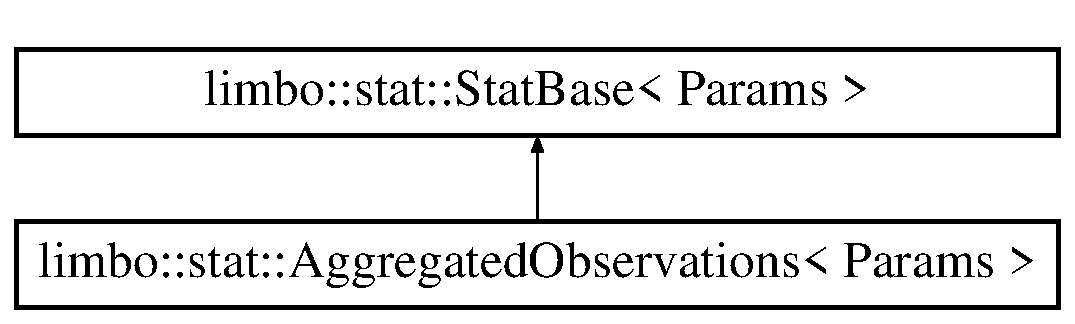
\includegraphics[height=2.000000cm]{structlimbo_1_1stat_1_1_aggregated_observations}
\end{center}
\end{figure}
\subsection*{Public Member Functions}
\begin{DoxyCompactItemize}
\item 
{\footnotesize template$<$typename B\+O , typename Aggregator\+Function $>$ }\\void \hyperlink{structlimbo_1_1stat_1_1_aggregated_observations_a99c53c6147e0d5ae26a7d4707a978611}{operator()} (const B\+O \&bo, const Aggregator\+Function \&afun)
\end{DoxyCompactItemize}


\subsection{Detailed Description}
\subsubsection*{template$<$typename Params$>$struct limbo\+::stat\+::\+Aggregated\+Observations$<$ Params $>$}

T\+O\+D\+O fallocati Write all the observations filename\+: {\ttfamily aggregated\+\_\+observations.\+dat} 

\subsection{Member Function Documentation}
\hypertarget{structlimbo_1_1stat_1_1_aggregated_observations_a99c53c6147e0d5ae26a7d4707a978611}{}\index{limbo\+::stat\+::\+Aggregated\+Observations@{limbo\+::stat\+::\+Aggregated\+Observations}!operator()@{operator()}}
\index{operator()@{operator()}!limbo\+::stat\+::\+Aggregated\+Observations@{limbo\+::stat\+::\+Aggregated\+Observations}}
\subsubsection[{operator()}]{\setlength{\rightskip}{0pt plus 5cm}template$<$typename Params $>$ template$<$typename B\+O , typename Aggregator\+Function $>$ void {\bf limbo\+::stat\+::\+Aggregated\+Observations}$<$ Params $>$\+::operator() (
\begin{DoxyParamCaption}
\item[{const B\+O \&}]{bo, }
\item[{const Aggregator\+Function \&}]{afun}
\end{DoxyParamCaption}
)\hspace{0.3cm}{\ttfamily [inline]}}\label{structlimbo_1_1stat_1_1_aggregated_observations_a99c53c6147e0d5ae26a7d4707a978611}


The documentation for this struct was generated from the following file\+:\begin{DoxyCompactItemize}
\item 
/tmp/doc\+\_\+limbo/limbo/src/limbo/stat/\hyperlink{aggregated__observations_8hpp}{aggregated\+\_\+observations.\+hpp}\end{DoxyCompactItemize}

\hypertarget{classrandutils_1_1auto__seeded}{}\section{randutils\+:\+:auto\+\_\+seeded$<$ Seed\+Seq $>$ Class Template Reference}
\label{classrandutils_1_1auto__seeded}\index{randutils\+::auto\+\_\+seeded$<$ Seed\+Seq $>$@{randutils\+::auto\+\_\+seeded$<$ Seed\+Seq $>$}}


{\ttfamily \#include $<$limbo/tools/rand\+\_\+utils.\+hpp$>$}

Inheritance diagram for randutils\+:\+:auto\+\_\+seeded$<$ Seed\+Seq $>$\+:\begin{figure}[H]
\begin{center}
\leavevmode
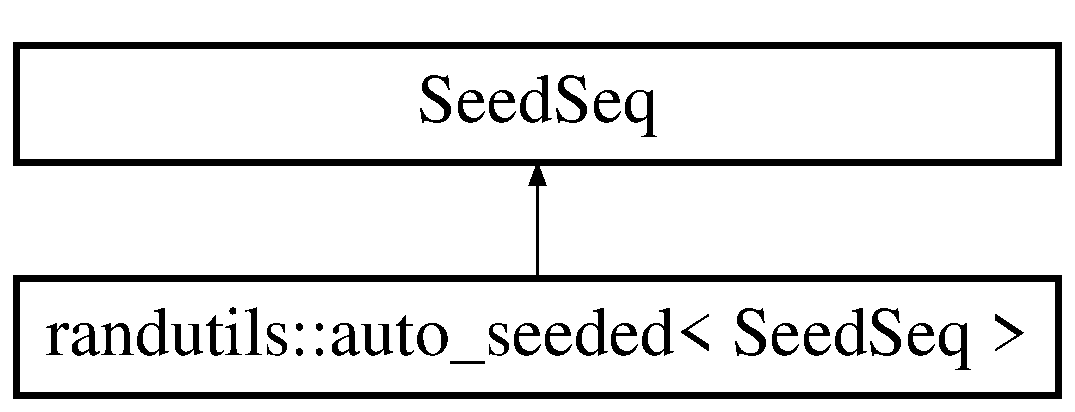
\includegraphics[height=2.000000cm]{classrandutils_1_1auto__seeded}
\end{center}
\end{figure}
\subsection*{Public Types}
\begin{DoxyCompactItemize}
\item 
using \hyperlink{classrandutils_1_1auto__seeded_a91549adccbb3c55e5d18b69c6647856f}{base\+\_\+seed\+\_\+seq} = Seed\+Seq
\end{DoxyCompactItemize}
\subsection*{Public Member Functions}
\begin{DoxyCompactItemize}
\item 
const \hyperlink{classrandutils_1_1auto__seeded_a91549adccbb3c55e5d18b69c6647856f}{base\+\_\+seed\+\_\+seq} \& \hyperlink{classrandutils_1_1auto__seeded_a632a62881c4ee2492a58920beb338074}{base} () const 
\item 
\hyperlink{classrandutils_1_1auto__seeded_a91549adccbb3c55e5d18b69c6647856f}{base\+\_\+seed\+\_\+seq} \& \hyperlink{classrandutils_1_1auto__seeded_af77746278c7d80a81f57912d0c4431f0}{base} ()
\item 
\hyperlink{classrandutils_1_1auto__seeded_a2d3b3febda1981eb6637f6b1ce535c87}{auto\+\_\+seeded} (default\+\_\+seeds seeds)
\item 
\hyperlink{classrandutils_1_1auto__seeded_a57acbed4b30b44634419a24fb866cbaf}{auto\+\_\+seeded} ()
\end{DoxyCompactItemize}


\subsection{Member Typedef Documentation}
\index{randutils\+::auto\+\_\+seeded@{randutils\+::auto\+\_\+seeded}!base\+\_\+seed\+\_\+seq@{base\+\_\+seed\+\_\+seq}}
\index{base\+\_\+seed\+\_\+seq@{base\+\_\+seed\+\_\+seq}!randutils\+::auto\+\_\+seeded@{randutils\+::auto\+\_\+seeded}}
\subsubsection[{\texorpdfstring{base\+\_\+seed\+\_\+seq}{base_seed_seq}}]{\setlength{\rightskip}{0pt plus 5cm}template$<$typename Seed\+Seq $>$ using {\bf randutils\+::auto\+\_\+seeded}$<$ Seed\+Seq $>$\+::{\bf base\+\_\+seed\+\_\+seq} =  Seed\+Seq}\hypertarget{classrandutils_1_1auto__seeded_a91549adccbb3c55e5d18b69c6647856f}{}\label{classrandutils_1_1auto__seeded_a91549adccbb3c55e5d18b69c6647856f}


\subsection{Constructor \& Destructor Documentation}
\index{randutils\+::auto\+\_\+seeded@{randutils\+::auto\+\_\+seeded}!auto\+\_\+seeded@{auto\+\_\+seeded}}
\index{auto\+\_\+seeded@{auto\+\_\+seeded}!randutils\+::auto\+\_\+seeded@{randutils\+::auto\+\_\+seeded}}
\subsubsection[{\texorpdfstring{auto\+\_\+seeded(default\+\_\+seeds seeds)}{auto_seeded(default_seeds seeds)}}]{\setlength{\rightskip}{0pt plus 5cm}template$<$typename Seed\+Seq $>$ {\bf randutils\+::auto\+\_\+seeded}$<$ Seed\+Seq $>$\+::{\bf auto\+\_\+seeded} (
\begin{DoxyParamCaption}
\item[{default\+\_\+seeds}]{seeds}
\end{DoxyParamCaption}
)\hspace{0.3cm}{\ttfamily [inline]}}\hypertarget{classrandutils_1_1auto__seeded_a2d3b3febda1981eb6637f6b1ce535c87}{}\label{classrandutils_1_1auto__seeded_a2d3b3febda1981eb6637f6b1ce535c87}
\index{randutils\+::auto\+\_\+seeded@{randutils\+::auto\+\_\+seeded}!auto\+\_\+seeded@{auto\+\_\+seeded}}
\index{auto\+\_\+seeded@{auto\+\_\+seeded}!randutils\+::auto\+\_\+seeded@{randutils\+::auto\+\_\+seeded}}
\subsubsection[{\texorpdfstring{auto\+\_\+seeded()}{auto_seeded()}}]{\setlength{\rightskip}{0pt plus 5cm}template$<$typename Seed\+Seq $>$ {\bf randutils\+::auto\+\_\+seeded}$<$ Seed\+Seq $>$\+::{\bf auto\+\_\+seeded} (
\begin{DoxyParamCaption}
{}
\end{DoxyParamCaption}
)\hspace{0.3cm}{\ttfamily [inline]}}\hypertarget{classrandutils_1_1auto__seeded_a57acbed4b30b44634419a24fb866cbaf}{}\label{classrandutils_1_1auto__seeded_a57acbed4b30b44634419a24fb866cbaf}


\subsection{Member Function Documentation}
\index{randutils\+::auto\+\_\+seeded@{randutils\+::auto\+\_\+seeded}!base@{base}}
\index{base@{base}!randutils\+::auto\+\_\+seeded@{randutils\+::auto\+\_\+seeded}}
\subsubsection[{\texorpdfstring{base() const }{base() const }}]{\setlength{\rightskip}{0pt plus 5cm}template$<$typename Seed\+Seq $>$ const {\bf base\+\_\+seed\+\_\+seq}\& {\bf randutils\+::auto\+\_\+seeded}$<$ Seed\+Seq $>$\+::base (
\begin{DoxyParamCaption}
{}
\end{DoxyParamCaption}
) const\hspace{0.3cm}{\ttfamily [inline]}}\hypertarget{classrandutils_1_1auto__seeded_a632a62881c4ee2492a58920beb338074}{}\label{classrandutils_1_1auto__seeded_a632a62881c4ee2492a58920beb338074}
\index{randutils\+::auto\+\_\+seeded@{randutils\+::auto\+\_\+seeded}!base@{base}}
\index{base@{base}!randutils\+::auto\+\_\+seeded@{randutils\+::auto\+\_\+seeded}}
\subsubsection[{\texorpdfstring{base()}{base()}}]{\setlength{\rightskip}{0pt plus 5cm}template$<$typename Seed\+Seq $>$ {\bf base\+\_\+seed\+\_\+seq}\& {\bf randutils\+::auto\+\_\+seeded}$<$ Seed\+Seq $>$\+::base (
\begin{DoxyParamCaption}
{}
\end{DoxyParamCaption}
)\hspace{0.3cm}{\ttfamily [inline]}}\hypertarget{classrandutils_1_1auto__seeded_af77746278c7d80a81f57912d0c4431f0}{}\label{classrandutils_1_1auto__seeded_af77746278c7d80a81f57912d0c4431f0}


The documentation for this class was generated from the following file\+:\begin{DoxyCompactItemize}
\item 
/tmp/doc\+\_\+limbo/limbo/src/limbo/tools/\hyperlink{rand__utils_8hpp}{rand\+\_\+utils.\+hpp}\end{DoxyCompactItemize}

\hypertarget{structlimbo_1_1defaults_1_1bayes__opt__bobase}{}\section{limbo\+:\+:defaults\+:\+:bayes\+\_\+opt\+\_\+bobase Struct Reference}
\label{structlimbo_1_1defaults_1_1bayes__opt__bobase}\index{limbo\+::defaults\+::bayes\+\_\+opt\+\_\+bobase@{limbo\+::defaults\+::bayes\+\_\+opt\+\_\+bobase}}


{\ttfamily \#include $<$limbo/bayes\+\_\+opt/bo\+\_\+base.\+hpp$>$}

\subsection*{Public Member Functions}
\begin{DoxyCompactItemize}
\item 
\hyperlink{structlimbo_1_1defaults_1_1bayes__opt__bobase_ae45d5d0172acb6ca307cb62e3fa35365}{B\+O\+\_\+\+P\+A\+R\+A\+M} (bool, stats\+\_\+enabled, true)
\end{DoxyCompactItemize}


\subsection{Member Function Documentation}
\hypertarget{structlimbo_1_1defaults_1_1bayes__opt__bobase_ae45d5d0172acb6ca307cb62e3fa35365}{}\index{limbo\+::defaults\+::bayes\+\_\+opt\+\_\+bobase@{limbo\+::defaults\+::bayes\+\_\+opt\+\_\+bobase}!B\+O\+\_\+\+P\+A\+R\+A\+M@{B\+O\+\_\+\+P\+A\+R\+A\+M}}
\index{B\+O\+\_\+\+P\+A\+R\+A\+M@{B\+O\+\_\+\+P\+A\+R\+A\+M}!limbo\+::defaults\+::bayes\+\_\+opt\+\_\+bobase@{limbo\+::defaults\+::bayes\+\_\+opt\+\_\+bobase}}
\subsubsection[{B\+O\+\_\+\+P\+A\+R\+A\+M}]{\setlength{\rightskip}{0pt plus 5cm}limbo\+::defaults\+::bayes\+\_\+opt\+\_\+bobase\+::\+B\+O\+\_\+\+P\+A\+R\+A\+M (
\begin{DoxyParamCaption}
\item[{bool}]{, }
\item[{stats\+\_\+enabled}]{, }
\item[{true}]{}
\end{DoxyParamCaption}
)}\label{structlimbo_1_1defaults_1_1bayes__opt__bobase_ae45d5d0172acb6ca307cb62e3fa35365}


The documentation for this struct was generated from the following file\+:\begin{DoxyCompactItemize}
\item 
/tmp/doc\+\_\+limbo/limbo/src/limbo/bayes\+\_\+opt/\hyperlink{bo__base_8hpp}{bo\+\_\+base.\+hpp}\end{DoxyCompactItemize}

\hypertarget{structlimbo_1_1defaults_1_1bayes__opt__boptimizer}{}\section{limbo\+:\+:defaults\+:\+:bayes\+\_\+opt\+\_\+boptimizer Struct Reference}
\label{structlimbo_1_1defaults_1_1bayes__opt__boptimizer}\index{limbo\+::defaults\+::bayes\+\_\+opt\+\_\+boptimizer@{limbo\+::defaults\+::bayes\+\_\+opt\+\_\+boptimizer}}


{\ttfamily \#include $<$limbo/bayes\+\_\+opt/boptimizer.\+hpp$>$}

\subsection*{Public Member Functions}
\begin{DoxyCompactItemize}
\item 
\hyperlink{structlimbo_1_1defaults_1_1bayes__opt__boptimizer_a20e662092603c59dc5f72bdda49c19a2}{B\+O\+\_\+\+P\+A\+R\+A\+M} (double, noise, 1e-\/6)
\end{DoxyCompactItemize}


\subsection{Member Function Documentation}
\hypertarget{structlimbo_1_1defaults_1_1bayes__opt__boptimizer_a20e662092603c59dc5f72bdda49c19a2}{}\index{limbo\+::defaults\+::bayes\+\_\+opt\+\_\+boptimizer@{limbo\+::defaults\+::bayes\+\_\+opt\+\_\+boptimizer}!B\+O\+\_\+\+P\+A\+R\+A\+M@{B\+O\+\_\+\+P\+A\+R\+A\+M}}
\index{B\+O\+\_\+\+P\+A\+R\+A\+M@{B\+O\+\_\+\+P\+A\+R\+A\+M}!limbo\+::defaults\+::bayes\+\_\+opt\+\_\+boptimizer@{limbo\+::defaults\+::bayes\+\_\+opt\+\_\+boptimizer}}
\subsubsection[{B\+O\+\_\+\+P\+A\+R\+A\+M}]{\setlength{\rightskip}{0pt plus 5cm}limbo\+::defaults\+::bayes\+\_\+opt\+\_\+boptimizer\+::\+B\+O\+\_\+\+P\+A\+R\+A\+M (
\begin{DoxyParamCaption}
\item[{double}]{, }
\item[{noise}]{, }
\item[{1e-\/}]{6}
\end{DoxyParamCaption}
)}\label{structlimbo_1_1defaults_1_1bayes__opt__boptimizer_a20e662092603c59dc5f72bdda49c19a2}


The documentation for this struct was generated from the following file\+:\begin{DoxyCompactItemize}
\item 
/tmp/doc\+\_\+limbo/limbo/src/limbo/bayes\+\_\+opt/\hyperlink{boptimizer_8hpp}{boptimizer.\+hpp}\end{DoxyCompactItemize}

\hypertarget{structlimbo_1_1defaults_1_1bayes__opt__ehvi}{}\section{limbo\+:\+:defaults\+:\+:bayes\+\_\+opt\+\_\+ehvi Struct Reference}
\label{structlimbo_1_1defaults_1_1bayes__opt__ehvi}\index{limbo\+::defaults\+::bayes\+\_\+opt\+\_\+ehvi@{limbo\+::defaults\+::bayes\+\_\+opt\+\_\+ehvi}}


{\ttfamily \#include $<$limbo/experimental/bayes\+\_\+opt/ehvi.\+hpp$>$}

\subsection*{Public Member Functions}
\begin{DoxyCompactItemize}
\item 
\hyperlink{structlimbo_1_1defaults_1_1bayes__opt__ehvi_a1cb97e82bdc2c50e649cdff5f7869efc}{B\+O\+\_\+\+P\+A\+R\+A\+M} (double, x\+\_\+ref,-\/11)
\item 
\hyperlink{structlimbo_1_1defaults_1_1bayes__opt__ehvi_a179aea9e746c90b2b542b020fe55d64d}{B\+O\+\_\+\+P\+A\+R\+A\+M} (double, y\+\_\+ref,-\/11)
\end{DoxyCompactItemize}


\subsection{Member Function Documentation}
\hypertarget{structlimbo_1_1defaults_1_1bayes__opt__ehvi_a1cb97e82bdc2c50e649cdff5f7869efc}{}\index{limbo\+::defaults\+::bayes\+\_\+opt\+\_\+ehvi@{limbo\+::defaults\+::bayes\+\_\+opt\+\_\+ehvi}!B\+O\+\_\+\+P\+A\+R\+A\+M@{B\+O\+\_\+\+P\+A\+R\+A\+M}}
\index{B\+O\+\_\+\+P\+A\+R\+A\+M@{B\+O\+\_\+\+P\+A\+R\+A\+M}!limbo\+::defaults\+::bayes\+\_\+opt\+\_\+ehvi@{limbo\+::defaults\+::bayes\+\_\+opt\+\_\+ehvi}}
\subsubsection[{B\+O\+\_\+\+P\+A\+R\+A\+M}]{\setlength{\rightskip}{0pt plus 5cm}limbo\+::defaults\+::bayes\+\_\+opt\+\_\+ehvi\+::\+B\+O\+\_\+\+P\+A\+R\+A\+M (
\begin{DoxyParamCaption}
\item[{double}]{, }
\item[{x\+\_\+ref}]{, }
\item[{-\/}]{11}
\end{DoxyParamCaption}
)}\label{structlimbo_1_1defaults_1_1bayes__opt__ehvi_a1cb97e82bdc2c50e649cdff5f7869efc}
\hypertarget{structlimbo_1_1defaults_1_1bayes__opt__ehvi_a179aea9e746c90b2b542b020fe55d64d}{}\index{limbo\+::defaults\+::bayes\+\_\+opt\+\_\+ehvi@{limbo\+::defaults\+::bayes\+\_\+opt\+\_\+ehvi}!B\+O\+\_\+\+P\+A\+R\+A\+M@{B\+O\+\_\+\+P\+A\+R\+A\+M}}
\index{B\+O\+\_\+\+P\+A\+R\+A\+M@{B\+O\+\_\+\+P\+A\+R\+A\+M}!limbo\+::defaults\+::bayes\+\_\+opt\+\_\+ehvi@{limbo\+::defaults\+::bayes\+\_\+opt\+\_\+ehvi}}
\subsubsection[{B\+O\+\_\+\+P\+A\+R\+A\+M}]{\setlength{\rightskip}{0pt plus 5cm}limbo\+::defaults\+::bayes\+\_\+opt\+\_\+ehvi\+::\+B\+O\+\_\+\+P\+A\+R\+A\+M (
\begin{DoxyParamCaption}
\item[{double}]{, }
\item[{y\+\_\+ref}]{, }
\item[{-\/}]{11}
\end{DoxyParamCaption}
)}\label{structlimbo_1_1defaults_1_1bayes__opt__ehvi_a179aea9e746c90b2b542b020fe55d64d}


The documentation for this struct was generated from the following file\+:\begin{DoxyCompactItemize}
\item 
/tmp/doc\+\_\+limbo/limbo/src/limbo/experimental/bayes\+\_\+opt/\hyperlink{bayes__opt_2ehvi_8hpp}{ehvi.\+hpp}\end{DoxyCompactItemize}

\hypertarget{structlimbo_1_1bayes__opt_1_1experimental_1_1defaults_1_1bayes__opt__imgpo}{}\section{limbo\+:\+:bayes\+\_\+opt\+:\+:experimental\+:\+:defaults\+:\+:bayes\+\_\+opt\+\_\+imgpo Struct Reference}
\label{structlimbo_1_1bayes__opt_1_1experimental_1_1defaults_1_1bayes__opt__imgpo}\index{limbo\+::bayes\+\_\+opt\+::experimental\+::defaults\+::bayes\+\_\+opt\+\_\+imgpo@{limbo\+::bayes\+\_\+opt\+::experimental\+::defaults\+::bayes\+\_\+opt\+\_\+imgpo}}


{\ttfamily \#include $<$limbo/experimental/bayes\+\_\+opt/imgpo.\+hpp$>$}

\subsection*{Public Member Functions}
\begin{DoxyCompactItemize}
\item 
\hyperlink{structlimbo_1_1bayes__opt_1_1experimental_1_1defaults_1_1bayes__opt__imgpo_a51a05f33be921d51d35262b305c6173b}{B\+O\+\_\+\+P\+A\+R\+AM} (double, noise, 1e-\/6)
\end{DoxyCompactItemize}


\subsection{Member Function Documentation}
\index{limbo\+::bayes\+\_\+opt\+::experimental\+::defaults\+::bayes\+\_\+opt\+\_\+imgpo@{limbo\+::bayes\+\_\+opt\+::experimental\+::defaults\+::bayes\+\_\+opt\+\_\+imgpo}!B\+O\+\_\+\+P\+A\+R\+AM@{B\+O\+\_\+\+P\+A\+R\+AM}}
\index{B\+O\+\_\+\+P\+A\+R\+AM@{B\+O\+\_\+\+P\+A\+R\+AM}!limbo\+::bayes\+\_\+opt\+::experimental\+::defaults\+::bayes\+\_\+opt\+\_\+imgpo@{limbo\+::bayes\+\_\+opt\+::experimental\+::defaults\+::bayes\+\_\+opt\+\_\+imgpo}}
\subsubsection[{\texorpdfstring{B\+O\+\_\+\+P\+A\+R\+A\+M(double, noise, 1e-\/6)}{BO_PARAM(double, noise, 1e-6)}}]{\setlength{\rightskip}{0pt plus 5cm}limbo\+::bayes\+\_\+opt\+::experimental\+::defaults\+::bayes\+\_\+opt\+\_\+imgpo\+::\+B\+O\+\_\+\+P\+A\+R\+AM (
\begin{DoxyParamCaption}
\item[{double}]{, }
\item[{noise}]{, }
\item[{1e-\/}]{6}
\end{DoxyParamCaption}
)}\hypertarget{structlimbo_1_1bayes__opt_1_1experimental_1_1defaults_1_1bayes__opt__imgpo_a51a05f33be921d51d35262b305c6173b}{}\label{structlimbo_1_1bayes__opt_1_1experimental_1_1defaults_1_1bayes__opt__imgpo_a51a05f33be921d51d35262b305c6173b}


The documentation for this struct was generated from the following file\+:\begin{DoxyCompactItemize}
\item 
/tmp/doc\+\_\+limbo/limbo/src/limbo/experimental/bayes\+\_\+opt/\hyperlink{imgpo_8hpp}{imgpo.\+hpp}\end{DoxyCompactItemize}

\hypertarget{structlimbo_1_1stat_1_1_best_aggregated_observations}{}\section{limbo\+:\+:stat\+:\+:Best\+Aggregated\+Observations$<$ Params $>$ Struct Template Reference}
\label{structlimbo_1_1stat_1_1_best_aggregated_observations}\index{limbo\+::stat\+::\+Best\+Aggregated\+Observations$<$ Params $>$@{limbo\+::stat\+::\+Best\+Aggregated\+Observations$<$ Params $>$}}


{\ttfamily \#include $<$limbo/stat/best\+\_\+aggregated\+\_\+observations.\+hpp$>$}

Inheritance diagram for limbo\+:\+:stat\+:\+:Best\+Aggregated\+Observations$<$ Params $>$\+:\begin{figure}[H]
\begin{center}
\leavevmode
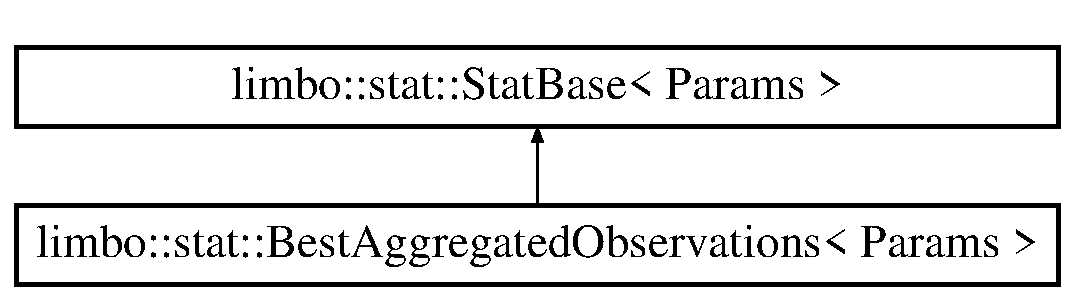
\includegraphics[height=2.000000cm]{structlimbo_1_1stat_1_1_best_aggregated_observations}
\end{center}
\end{figure}
\subsection*{Public Member Functions}
\begin{DoxyCompactItemize}
\item 
{\footnotesize template$<$typename BO , typename Aggregator\+Function $>$ }\\void \hyperlink{structlimbo_1_1stat_1_1_best_aggregated_observations_a37ad22cd25f49bbec5109a6f1367057e}{operator()} (const BO \&bo, const Aggregator\+Function \&afun)
\end{DoxyCompactItemize}


\subsection{Detailed Description}
\subsubsection*{template$<$typename Params$>$\\*
struct limbo\+::stat\+::\+Best\+Aggregated\+Observations$<$ Params $>$}

T\+O\+DO fallocati Write the best observation at each iteration filename\+: {\ttfamily best\+\_\+aggregated\+\_\+observations.\+dat} 

\subsection{Member Function Documentation}
\index{limbo\+::stat\+::\+Best\+Aggregated\+Observations@{limbo\+::stat\+::\+Best\+Aggregated\+Observations}!operator()@{operator()}}
\index{operator()@{operator()}!limbo\+::stat\+::\+Best\+Aggregated\+Observations@{limbo\+::stat\+::\+Best\+Aggregated\+Observations}}
\subsubsection[{\texorpdfstring{operator()(const B\+O \&bo, const Aggregator\+Function \&afun)}{operator()(const BO &bo, const AggregatorFunction &afun)}}]{\setlength{\rightskip}{0pt plus 5cm}template$<$typename Params $>$ template$<$typename BO , typename Aggregator\+Function $>$ void {\bf limbo\+::stat\+::\+Best\+Aggregated\+Observations}$<$ Params $>$\+::operator() (
\begin{DoxyParamCaption}
\item[{const BO \&}]{bo, }
\item[{const Aggregator\+Function \&}]{afun}
\end{DoxyParamCaption}
)\hspace{0.3cm}{\ttfamily [inline]}}\hypertarget{structlimbo_1_1stat_1_1_best_aggregated_observations_a37ad22cd25f49bbec5109a6f1367057e}{}\label{structlimbo_1_1stat_1_1_best_aggregated_observations_a37ad22cd25f49bbec5109a6f1367057e}


The documentation for this struct was generated from the following file\+:\begin{DoxyCompactItemize}
\item 
/tmp/doc\+\_\+limbo/limbo/src/limbo/stat/\hyperlink{best__aggregated__observations_8hpp}{best\+\_\+aggregated\+\_\+observations.\+hpp}\end{DoxyCompactItemize}

\hypertarget{structlimbo_1_1stat_1_1_best_observations}{}\section{limbo\+:\+:stat\+:\+:Best\+Observations$<$ Params $>$ Struct Template Reference}
\label{structlimbo_1_1stat_1_1_best_observations}\index{limbo\+::stat\+::\+Best\+Observations$<$ Params $>$@{limbo\+::stat\+::\+Best\+Observations$<$ Params $>$}}


{\ttfamily \#include $<$limbo/stat/best\+\_\+observations.\+hpp$>$}

Inheritance diagram for limbo\+:\+:stat\+:\+:Best\+Observations$<$ Params $>$\+:\begin{figure}[H]
\begin{center}
\leavevmode
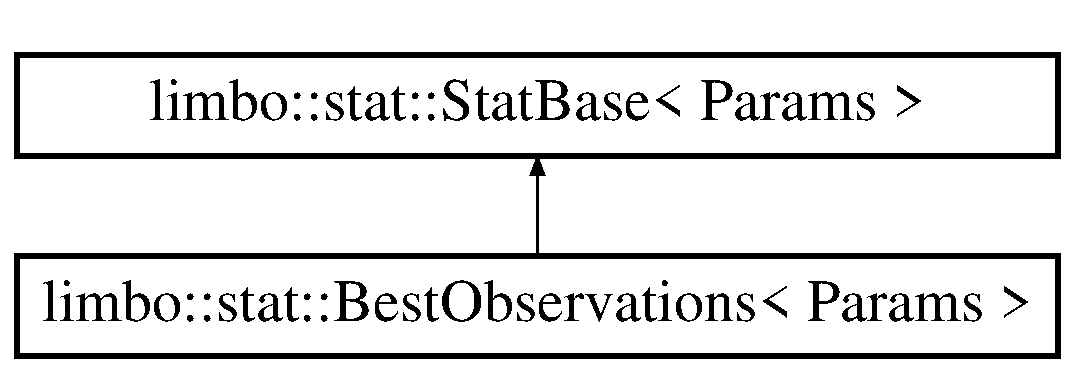
\includegraphics[height=2.000000cm]{structlimbo_1_1stat_1_1_best_observations}
\end{center}
\end{figure}
\subsection*{Public Member Functions}
\begin{DoxyCompactItemize}
\item 
{\footnotesize template$<$typename B\+O , typename Aggregator\+Function $>$ }\\void \hyperlink{structlimbo_1_1stat_1_1_best_observations_a62490e2a957d770d30c8575e1c34ce76}{operator()} (const B\+O \&bo, const Aggregator\+Function \&afun, bool blacklisted)
\end{DoxyCompactItemize}


\subsection{Detailed Description}
\subsubsection*{template$<$typename Params$>$struct limbo\+::stat\+::\+Best\+Observations$<$ Params $>$}

Write the best observation so far filename\+: {\ttfamily best\+\_\+observations.\+dat"} 

\subsection{Member Function Documentation}
\hypertarget{structlimbo_1_1stat_1_1_best_observations_a62490e2a957d770d30c8575e1c34ce76}{}\index{limbo\+::stat\+::\+Best\+Observations@{limbo\+::stat\+::\+Best\+Observations}!operator()@{operator()}}
\index{operator()@{operator()}!limbo\+::stat\+::\+Best\+Observations@{limbo\+::stat\+::\+Best\+Observations}}
\subsubsection[{operator()}]{\setlength{\rightskip}{0pt plus 5cm}template$<$typename Params $>$ template$<$typename B\+O , typename Aggregator\+Function $>$ void {\bf limbo\+::stat\+::\+Best\+Observations}$<$ Params $>$\+::operator() (
\begin{DoxyParamCaption}
\item[{const B\+O \&}]{bo, }
\item[{const Aggregator\+Function \&}]{afun, }
\item[{bool}]{blacklisted}
\end{DoxyParamCaption}
)\hspace{0.3cm}{\ttfamily [inline]}}\label{structlimbo_1_1stat_1_1_best_observations_a62490e2a957d770d30c8575e1c34ce76}


The documentation for this struct was generated from the following file\+:\begin{DoxyCompactItemize}
\item 
/tmp/doc\+\_\+limbo/limbo/src/limbo/stat/\hyperlink{best__observations_8hpp}{best\+\_\+observations.\+hpp}\end{DoxyCompactItemize}

\hypertarget{structlimbo_1_1stat_1_1_best_samples}{}\section{limbo\+:\+:stat\+:\+:Best\+Samples$<$ Params $>$ Struct Template Reference}
\label{structlimbo_1_1stat_1_1_best_samples}\index{limbo\+::stat\+::\+Best\+Samples$<$ Params $>$@{limbo\+::stat\+::\+Best\+Samples$<$ Params $>$}}


{\ttfamily \#include $<$limbo/stat/best\+\_\+samples.\+hpp$>$}

Inheritance diagram for limbo\+:\+:stat\+:\+:Best\+Samples$<$ Params $>$\+:\begin{figure}[H]
\begin{center}
\leavevmode
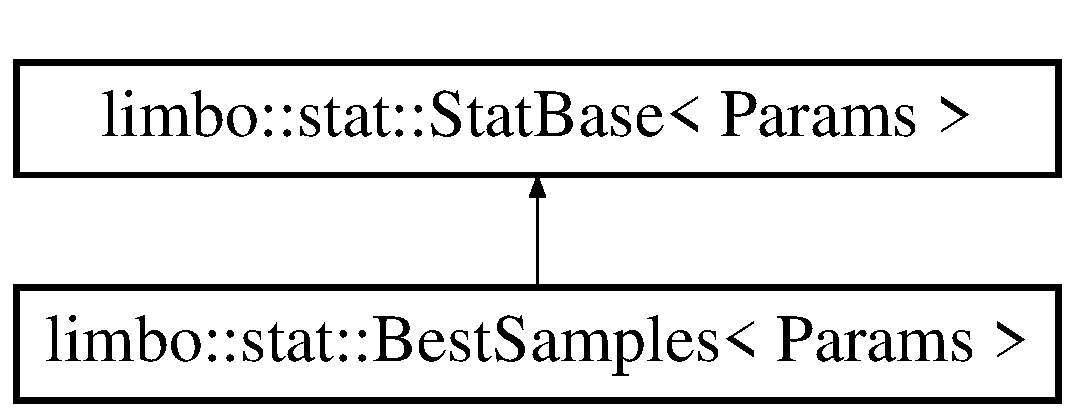
\includegraphics[height=2.000000cm]{structlimbo_1_1stat_1_1_best_samples}
\end{center}
\end{figure}
\subsection*{Public Member Functions}
\begin{DoxyCompactItemize}
\item 
{\footnotesize template$<$typename BO , typename Aggregator\+Function $>$ }\\void \hyperlink{structlimbo_1_1stat_1_1_best_samples_a432216d8c0eaeca98226e500c304e5fa}{operator()} (const BO \&bo, const Aggregator\+Function \&afun)
\end{DoxyCompactItemize}


\subsection{Detailed Description}
\subsubsection*{template$<$typename Params$>$\\*
struct limbo\+::stat\+::\+Best\+Samples$<$ Params $>$}

filename\+: {\ttfamily best\+\_\+samples.\+dat} 

\subsection{Member Function Documentation}
\index{limbo\+::stat\+::\+Best\+Samples@{limbo\+::stat\+::\+Best\+Samples}!operator()@{operator()}}
\index{operator()@{operator()}!limbo\+::stat\+::\+Best\+Samples@{limbo\+::stat\+::\+Best\+Samples}}
\subsubsection[{\texorpdfstring{operator()(const B\+O \&bo, const Aggregator\+Function \&afun)}{operator()(const BO &bo, const AggregatorFunction &afun)}}]{\setlength{\rightskip}{0pt plus 5cm}template$<$typename Params $>$ template$<$typename BO , typename Aggregator\+Function $>$ void {\bf limbo\+::stat\+::\+Best\+Samples}$<$ Params $>$\+::operator() (
\begin{DoxyParamCaption}
\item[{const BO \&}]{bo, }
\item[{const Aggregator\+Function \&}]{afun}
\end{DoxyParamCaption}
)\hspace{0.3cm}{\ttfamily [inline]}}\hypertarget{structlimbo_1_1stat_1_1_best_samples_a432216d8c0eaeca98226e500c304e5fa}{}\label{structlimbo_1_1stat_1_1_best_samples_a432216d8c0eaeca98226e500c304e5fa}


The documentation for this struct was generated from the following file\+:\begin{DoxyCompactItemize}
\item 
/tmp/doc\+\_\+limbo/limbo/src/limbo/stat/\hyperlink{best__samples_8hpp}{best\+\_\+samples.\+hpp}\end{DoxyCompactItemize}

\hypertarget{structlimbo_1_1stat_1_1_bl_samples}{}\section{limbo\+:\+:stat\+:\+:Bl\+Samples$<$ Params $>$ Struct Template Reference}
\label{structlimbo_1_1stat_1_1_bl_samples}\index{limbo\+::stat\+::\+Bl\+Samples$<$ Params $>$@{limbo\+::stat\+::\+Bl\+Samples$<$ Params $>$}}


{\ttfamily \#include $<$limbo/stat/bl\+\_\+samples.\+hpp$>$}

Inheritance diagram for limbo\+:\+:stat\+:\+:Bl\+Samples$<$ Params $>$\+:\begin{figure}[H]
\begin{center}
\leavevmode
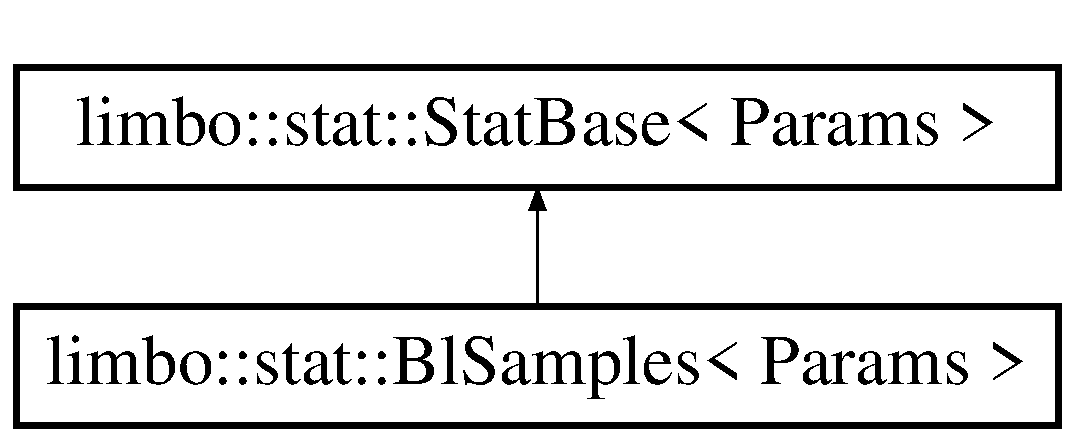
\includegraphics[height=2.000000cm]{structlimbo_1_1stat_1_1_bl_samples}
\end{center}
\end{figure}
\subsection*{Public Member Functions}
\begin{DoxyCompactItemize}
\item 
{\footnotesize template$<$typename B\+O , typename Aggregator\+Function $>$ }\\void \hyperlink{structlimbo_1_1stat_1_1_bl_samples_a1671492ad1724364555d5b042cd81d15}{operator()} (const B\+O \&bo, const Aggregator\+Function \&, bool blacklisted)
\end{DoxyCompactItemize}


\subsection{Detailed Description}
\subsubsection*{template$<$typename Params$>$struct limbo\+::stat\+::\+Bl\+Samples$<$ Params $>$}

blacklisted samples filename\+: {\ttfamily bl\+\_\+samples.\+dat} 

\subsection{Member Function Documentation}
\hypertarget{structlimbo_1_1stat_1_1_bl_samples_a1671492ad1724364555d5b042cd81d15}{}\index{limbo\+::stat\+::\+Bl\+Samples@{limbo\+::stat\+::\+Bl\+Samples}!operator()@{operator()}}
\index{operator()@{operator()}!limbo\+::stat\+::\+Bl\+Samples@{limbo\+::stat\+::\+Bl\+Samples}}
\subsubsection[{operator()}]{\setlength{\rightskip}{0pt plus 5cm}template$<$typename Params $>$ template$<$typename B\+O , typename Aggregator\+Function $>$ void {\bf limbo\+::stat\+::\+Bl\+Samples}$<$ Params $>$\+::operator() (
\begin{DoxyParamCaption}
\item[{const B\+O \&}]{bo, }
\item[{const Aggregator\+Function \&}]{, }
\item[{bool}]{blacklisted}
\end{DoxyParamCaption}
)\hspace{0.3cm}{\ttfamily [inline]}}\label{structlimbo_1_1stat_1_1_bl_samples_a1671492ad1724364555d5b042cd81d15}


The documentation for this struct was generated from the following file\+:\begin{DoxyCompactItemize}
\item 
/tmp/doc\+\_\+limbo/limbo/src/limbo/stat/\hyperlink{bl__samples_8hpp}{bl\+\_\+samples.\+hpp}\end{DoxyCompactItemize}

\hypertarget{classlimbo_1_1bayes__opt_1_1_bo_base}{}\section{limbo\+:\+:bayes\+\_\+opt\+:\+:Bo\+Base$<$ Params, A1, A2, A3, A4, A5, A6 $>$ Class Template Reference}
\label{classlimbo_1_1bayes__opt_1_1_bo_base}\index{limbo\+::bayes\+\_\+opt\+::\+Bo\+Base$<$ Params, A1, A2, A3, A4, A5, A6 $>$@{limbo\+::bayes\+\_\+opt\+::\+Bo\+Base$<$ Params, A1, A2, A3, A4, A5, A6 $>$}}


{\ttfamily \#include $<$limbo/bayes\+\_\+opt/bo\+\_\+base.\+hpp$>$}

Inheritance diagram for limbo\+:\+:bayes\+\_\+opt\+:\+:Bo\+Base$<$ Params, A1, A2, A3, A4, A5, A6 $>$\+:\begin{figure}[H]
\begin{center}
\leavevmode
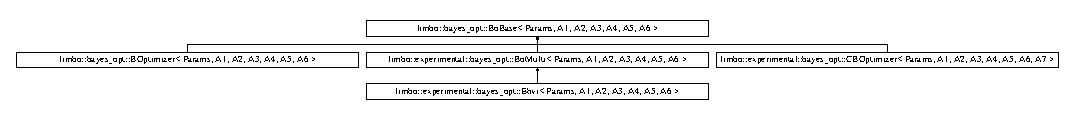
\includegraphics[height=2.000000cm]{classlimbo_1_1bayes__opt_1_1_bo_base}
\end{center}
\end{figure}
\subsection*{Classes}
\begin{DoxyCompactItemize}
\item 
struct \hyperlink{structlimbo_1_1bayes__opt_1_1_bo_base_1_1defaults}{defaults}
\end{DoxyCompactItemize}
\subsection*{Public Types}
\begin{DoxyCompactItemize}
\item 
typedef Params \hyperlink{classlimbo_1_1bayes__opt_1_1_bo_base_ae46fa6c574ca2a2c4368c8c9d3ff63e5}{params\+\_\+t}
\item 
typedef bobase\+\_\+signature\+::bind$<$ A1, A2, A3, A4, A5, A6 $>$\+::type \hyperlink{classlimbo_1_1bayes__opt_1_1_bo_base_a3844c259aa1e59d0241f90390aa6f7fa}{args}
\item 
typedef boost\+::parameter\+::binding$<$ \hyperlink{classlimbo_1_1bayes__opt_1_1_bo_base_a3844c259aa1e59d0241f90390aa6f7fa}{args}, tag\+::initfun, typename \hyperlink{structlimbo_1_1bayes__opt_1_1_bo_base_1_1defaults_a675d927a474fc77608cc63c8406448f7}{defaults\+::init\+\_\+t} $>$\+::type \hyperlink{classlimbo_1_1bayes__opt_1_1_bo_base_a734d263ce8c37ae2c5233f9e4499828c}{init\+\_\+function\+\_\+t}
\item 
typedef boost\+::parameter\+::binding$<$ \hyperlink{classlimbo_1_1bayes__opt_1_1_bo_base_a3844c259aa1e59d0241f90390aa6f7fa}{args}, tag\+::acquifun, typename \hyperlink{structlimbo_1_1bayes__opt_1_1_bo_base_1_1defaults_a4cb9b80ab762b3b763fdd97e893886e5}{defaults\+::acqui\+\_\+t} $>$\+::type \hyperlink{classlimbo_1_1bayes__opt_1_1_bo_base_a200a43abb6c95d2d99660898b36f2200}{acquisition\+\_\+function\+\_\+t}
\item 
typedef boost\+::parameter\+::binding$<$ \hyperlink{classlimbo_1_1bayes__opt_1_1_bo_base_a3844c259aa1e59d0241f90390aa6f7fa}{args}, tag\+::modelfun, typename \hyperlink{structlimbo_1_1bayes__opt_1_1_bo_base_1_1defaults_a07f65b6332c4f0c029069100feecb789}{defaults\+::model\+\_\+t} $>$\+::type \hyperlink{classlimbo_1_1bayes__opt_1_1_bo_base_a151af5c7eef92a82d8813bb2e067d267}{model\+\_\+t}
\item 
typedef boost\+::parameter\+::binding$<$ \hyperlink{classlimbo_1_1bayes__opt_1_1_bo_base_a3844c259aa1e59d0241f90390aa6f7fa}{args}, tag\+::statsfun, typename \hyperlink{structlimbo_1_1bayes__opt_1_1_bo_base_1_1defaults_ab8f3991474723d27b9c77d0e0a76fce2}{defaults\+::stat\+\_\+t} $>$\+::type \hyperlink{classlimbo_1_1bayes__opt_1_1_bo_base_adda0d6bf0fa0def996eb0af7e8a84f3f}{Stat}
\item 
typedef boost\+::parameter\+::binding$<$ \hyperlink{classlimbo_1_1bayes__opt_1_1_bo_base_a3844c259aa1e59d0241f90390aa6f7fa}{args}, tag\+::stopcrit, typename \hyperlink{structlimbo_1_1bayes__opt_1_1_bo_base_1_1defaults_a66e1dbe1ccd9dbef0fdfc5c9faee9eff}{defaults\+::stop\+\_\+t} $>$\+::type \hyperlink{classlimbo_1_1bayes__opt_1_1_bo_base_a06717d469296323cc277e3769b828e98}{Stopping\+Criteria}
\item 
typedef boost\+::mpl\+::if\+\_\+$<$ boost\+::fusion\+::traits\+::is\+\_\+sequence$<$ \hyperlink{classlimbo_1_1bayes__opt_1_1_bo_base_a06717d469296323cc277e3769b828e98}{Stopping\+Criteria} $>$, \hyperlink{classlimbo_1_1bayes__opt_1_1_bo_base_a06717d469296323cc277e3769b828e98}{Stopping\+Criteria}, boost\+::fusion\+::vector$<$ \hyperlink{classlimbo_1_1bayes__opt_1_1_bo_base_a06717d469296323cc277e3769b828e98}{Stopping\+Criteria} $>$ $>$\+::type \hyperlink{classlimbo_1_1bayes__opt_1_1_bo_base_a8dfcab20696e6c85665b150e9881c010}{stopping\+\_\+criteria\+\_\+t}
\item 
typedef boost\+::mpl\+::if\+\_\+$<$ boost\+::fusion\+::traits\+::is\+\_\+sequence$<$ \hyperlink{classlimbo_1_1bayes__opt_1_1_bo_base_adda0d6bf0fa0def996eb0af7e8a84f3f}{Stat} $>$, \hyperlink{classlimbo_1_1bayes__opt_1_1_bo_base_adda0d6bf0fa0def996eb0af7e8a84f3f}{Stat}, boost\+::fusion\+::vector$<$ \hyperlink{classlimbo_1_1bayes__opt_1_1_bo_base_adda0d6bf0fa0def996eb0af7e8a84f3f}{Stat} $>$ $>$\+::type \hyperlink{classlimbo_1_1bayes__opt_1_1_bo_base_a17d395abfdd3158f238c83764ba68fd0}{stat\+\_\+t}
\end{DoxyCompactItemize}
\subsection*{Public Member Functions}
\begin{DoxyCompactItemize}
\item 
\hyperlink{classlimbo_1_1bayes__opt_1_1_bo_base_ad361278c23693c4220eaa9a9de5d3333}{Bo\+Base} ()
\begin{DoxyCompactList}\small\item\em default constructor \end{DoxyCompactList}\item 
\hyperlink{classlimbo_1_1bayes__opt_1_1_bo_base_a1a50eebb8a6efd528582ea871a0879a0}{Bo\+Base} (const \hyperlink{classlimbo_1_1bayes__opt_1_1_bo_base}{Bo\+Base} \&other)=delete
\begin{DoxyCompactList}\small\item\em copy is disabled (dangerous and useless) \end{DoxyCompactList}\item 
\hyperlink{classlimbo_1_1bayes__opt_1_1_bo_base}{Bo\+Base} \& \hyperlink{classlimbo_1_1bayes__opt_1_1_bo_base_a69628ced9d71209a59dcdfb7f5637265}{operator=} (const \hyperlink{classlimbo_1_1bayes__opt_1_1_bo_base}{Bo\+Base} \&other)=delete
\begin{DoxyCompactList}\small\item\em copy is disabled (dangerous and useless) \end{DoxyCompactList}\item 
bool \hyperlink{classlimbo_1_1bayes__opt_1_1_bo_base_a4d94db5c40b35bec292aebfd19b8fb3d}{stats\+\_\+enabled} () const 
\begin{DoxyCompactList}\small\item\em return true if the statitics are enabled (they can be disabled to avoid dumping data, e.\+g. for unit tests) \end{DoxyCompactList}\item 
const std\+::string \& \hyperlink{classlimbo_1_1bayes__opt_1_1_bo_base_a4c87b7618144f99027c294db3eb803f6}{res\+\_\+dir} () const 
\begin{DoxyCompactList}\small\item\em return the name of the directory in which results (statistics) are written \end{DoxyCompactList}\item 
const std\+::vector$<$ Eigen\+::\+Vector\+Xd $>$ \& \hyperlink{classlimbo_1_1bayes__opt_1_1_bo_base_a855dc5de1d0732a25f4c9730ac50d0bd}{observations} () const 
\begin{DoxyCompactList}\small\item\em return the vector of points of observations (observations can be multi-\/dimensional, hence the Vector\+Xd) -- f(x) \end{DoxyCompactList}\item 
const std\+::vector$<$ Eigen\+::\+Vector\+Xd $>$ \& \hyperlink{classlimbo_1_1bayes__opt_1_1_bo_base_ad3ba0dba1418df0ed8e79d4dd3cc907a}{samples} () const 
\begin{DoxyCompactList}\small\item\em return the list of the points that have been evaluated so far (x) \end{DoxyCompactList}\item 
const std\+::vector$<$ Eigen\+::\+Vector\+Xd $>$ \& \hyperlink{classlimbo_1_1bayes__opt_1_1_bo_base_aa84e215cffa97a4e287aad3690f89635}{bl\+\_\+samples} () const 
\begin{DoxyCompactList}\small\item\em return the list of blacklisted points \end{DoxyCompactList}\item 
int \hyperlink{classlimbo_1_1bayes__opt_1_1_bo_base_ac3d643d5a668edf22ad053bfc54ea090}{current\+\_\+iteration} () const 
\begin{DoxyCompactList}\small\item\em return the current iteration number \end{DoxyCompactList}\item 
int \hyperlink{classlimbo_1_1bayes__opt_1_1_bo_base_a5470e106c4584a30636cafb6fbad6d73}{total\+\_\+iterations} () const 
\item 
void \hyperlink{classlimbo_1_1bayes__opt_1_1_bo_base_ac533d6397b0c0fa5ba0a4d03e0545fa2}{add\+\_\+new\+\_\+sample} (const Eigen\+::\+Vector\+Xd \&s, const Eigen\+::\+Vector\+Xd \&v)
\item 
void \hyperlink{classlimbo_1_1bayes__opt_1_1_bo_base_a8694d4bbc5c373d067790ec31fb42a44}{add\+\_\+new\+\_\+bl\+\_\+sample} (const Eigen\+::\+Vector\+Xd \&s)
\begin{DoxyCompactList}\small\item\em Add a new blacklisted sample. \end{DoxyCompactList}\item 
{\footnotesize template$<$typename State\+Function $>$ }\\bool \hyperlink{classlimbo_1_1bayes__opt_1_1_bo_base_a387fba7bf70aa9410e1c04f035694f34}{eval\+\_\+and\+\_\+add} (const State\+Function \&seval, const Eigen\+::\+Vector\+Xd \&sample)
\begin{DoxyCompactList}\small\item\em Evaluate a sample and add the result to the \textquotesingle{}database\textquotesingle{} (sample / observations vectors) -- it does not update the model. \end{DoxyCompactList}\end{DoxyCompactItemize}


\subsection{Detailed Description}
\subsubsection*{template$<$class Params, class A1 = boost\+::parameter\+::void\+\_\+, class A2 = boost\+::parameter\+::void\+\_\+, class A3 = boost\+::parameter\+::void\+\_\+, class A4 = boost\+::parameter\+::void\+\_\+, class A5 = boost\+::parameter\+::void\+\_\+, class A6 = boost\+::parameter\+::void\+\_\+$>$class limbo\+::bayes\+\_\+opt\+::\+Bo\+Base$<$ Params, A1, A2, A3, A4, A5, A6 $>$}

\begin{DoxyVerb}embed:rst

Base class for Bayesian optimizers

Parameters:
  - ``bool Params::bayes_opt_bobase::stats_enabled``: activate / deactivate the statistics

This class is templated by several types with default values (thanks to boost::parameters).

+----------------+---------+---------+---------------+
|type            |typedef  | argument| default       |
+================+=========+=========+===============+
|init. func.     |init_t   | initfun | RandomSampling|
+----------------+---------+---------+---------------+
|model           |model_t  | modelfun| GP<...>       |
+----------------+---------+---------+---------------+
|acquisition fun.|aqui_t   | acquifun| GP_UCB        |
+----------------+---------+---------+---------------+
|statistics      | stat_t  | statfun | see below     |
+----------------+---------+---------+---------------+
|stopping crit.  | stop_t  | stopcrit| MaxIterations |
+----------------+---------+---------+---------------+\end{DoxyVerb}


For G\+P, the default value is\+: {\ttfamily \hyperlink{classlimbo_1_1model_1_1_g_p}{model\+::\+G\+P}$<$Params, kf\+\_\+t, mean\+\_\+t, opt\+\_\+t$>$$>$},
\begin{DoxyItemize}
\item with {\ttfamily kf\+\_\+t = \hyperlink{structlimbo_1_1kernel_1_1_squared_exp_a_r_d}{kernel\+::\+Squared\+Exp\+A\+R\+D}$<$Params$>$}
\item with {\ttfamily mean\+\_\+t = \hyperlink{structlimbo_1_1mean_1_1_data}{mean\+::\+Data}$<$Params$>$}
\item with {\ttfamily opt\+\_\+t = \hyperlink{structlimbo_1_1model_1_1gp_1_1_kernel_l_f_opt}{model\+::gp\+::\+Kernel\+L\+F\+Opt}$<$Params$>$}
\end{DoxyItemize}

(meaning\+: kernel with automatic relevance determination and mean equals to the mean of the input data, that is, center the data automatically)

For Statistics, the default value is\+: {\ttfamily boost\+::fusion\+::vector$<$\hyperlink{structlimbo_1_1stat_1_1_samples}{stat\+::\+Samples}$<$Params$>$, \hyperlink{structlimbo_1_1stat_1_1_aggregated_observations}{stat\+::\+Aggregated\+Observations}$<$Params$>$, \hyperlink{structlimbo_1_1stat_1_1_console_summary}{stat\+::\+Console\+Summary}$<$Params$>$$>$}

Example of customization\+:
\begin{DoxyItemize}
\item {\ttfamily typedef \hyperlink{structlimbo_1_1kernel_1_1_matern_five_halfs}{kernel\+::\+Matern\+Five\+Halfs}$<$Params$>$ Kernel\+\_\+t;}
\item {\ttfamily typedef \hyperlink{structlimbo_1_1mean_1_1_data}{mean\+::\+Data}$<$Params$>$ Mean\+\_\+t;}
\item {\ttfamily typedef \hyperlink{classlimbo_1_1model_1_1_g_p}{model\+::\+G\+P}$<$Params, Kernel\+\_\+t, Mean\+\_\+t$>$ G\+P\+\_\+t;}
\item {\ttfamily typedef \hyperlink{classlimbo_1_1acqui_1_1_u_c_b}{acqui\+::\+U\+C\+B}$<$Params, G\+P\+\_\+t$>$ Acqui\+\_\+t;}
\item {\ttfamily \hyperlink{classlimbo_1_1bayes__opt_1_1_b_optimizer}{bayes\+\_\+opt\+::\+B\+Optimizer}$<$Params, modelfun$<$G\+P\+\_\+t$>$, acquifun$<$Acqui\+\_\+t$>$$>$ opt;} 
\end{DoxyItemize}

\subsection{Member Typedef Documentation}
\hypertarget{classlimbo_1_1bayes__opt_1_1_bo_base_a200a43abb6c95d2d99660898b36f2200}{}\index{limbo\+::bayes\+\_\+opt\+::\+Bo\+Base@{limbo\+::bayes\+\_\+opt\+::\+Bo\+Base}!acquisition\+\_\+function\+\_\+t@{acquisition\+\_\+function\+\_\+t}}
\index{acquisition\+\_\+function\+\_\+t@{acquisition\+\_\+function\+\_\+t}!limbo\+::bayes\+\_\+opt\+::\+Bo\+Base@{limbo\+::bayes\+\_\+opt\+::\+Bo\+Base}}
\subsubsection[{acquisition\+\_\+function\+\_\+t}]{\setlength{\rightskip}{0pt plus 5cm}template$<$class Params, class A1 = boost\+::parameter\+::void\+\_\+, class A2 = boost\+::parameter\+::void\+\_\+, class A3 = boost\+::parameter\+::void\+\_\+, class A4 = boost\+::parameter\+::void\+\_\+, class A5 = boost\+::parameter\+::void\+\_\+, class A6 = boost\+::parameter\+::void\+\_\+$>$ typedef boost\+::parameter\+::binding$<${\bf args}, tag\+::acquifun, typename {\bf defaults\+::acqui\+\_\+t}$>$\+::type {\bf limbo\+::bayes\+\_\+opt\+::\+Bo\+Base}$<$ Params, A1, A2, A3, A4, A5, A6 $>$\+::{\bf acquisition\+\_\+function\+\_\+t}}\label{classlimbo_1_1bayes__opt_1_1_bo_base_a200a43abb6c95d2d99660898b36f2200}
\hypertarget{classlimbo_1_1bayes__opt_1_1_bo_base_a3844c259aa1e59d0241f90390aa6f7fa}{}\index{limbo\+::bayes\+\_\+opt\+::\+Bo\+Base@{limbo\+::bayes\+\_\+opt\+::\+Bo\+Base}!args@{args}}
\index{args@{args}!limbo\+::bayes\+\_\+opt\+::\+Bo\+Base@{limbo\+::bayes\+\_\+opt\+::\+Bo\+Base}}
\subsubsection[{args}]{\setlength{\rightskip}{0pt plus 5cm}template$<$class Params, class A1 = boost\+::parameter\+::void\+\_\+, class A2 = boost\+::parameter\+::void\+\_\+, class A3 = boost\+::parameter\+::void\+\_\+, class A4 = boost\+::parameter\+::void\+\_\+, class A5 = boost\+::parameter\+::void\+\_\+, class A6 = boost\+::parameter\+::void\+\_\+$>$ typedef bobase\+\_\+signature\+::bind$<$A1, A2, A3, A4, A5, A6$>$\+::type {\bf limbo\+::bayes\+\_\+opt\+::\+Bo\+Base}$<$ Params, A1, A2, A3, A4, A5, A6 $>$\+::{\bf args}}\label{classlimbo_1_1bayes__opt_1_1_bo_base_a3844c259aa1e59d0241f90390aa6f7fa}
\hypertarget{classlimbo_1_1bayes__opt_1_1_bo_base_a734d263ce8c37ae2c5233f9e4499828c}{}\index{limbo\+::bayes\+\_\+opt\+::\+Bo\+Base@{limbo\+::bayes\+\_\+opt\+::\+Bo\+Base}!init\+\_\+function\+\_\+t@{init\+\_\+function\+\_\+t}}
\index{init\+\_\+function\+\_\+t@{init\+\_\+function\+\_\+t}!limbo\+::bayes\+\_\+opt\+::\+Bo\+Base@{limbo\+::bayes\+\_\+opt\+::\+Bo\+Base}}
\subsubsection[{init\+\_\+function\+\_\+t}]{\setlength{\rightskip}{0pt plus 5cm}template$<$class Params, class A1 = boost\+::parameter\+::void\+\_\+, class A2 = boost\+::parameter\+::void\+\_\+, class A3 = boost\+::parameter\+::void\+\_\+, class A4 = boost\+::parameter\+::void\+\_\+, class A5 = boost\+::parameter\+::void\+\_\+, class A6 = boost\+::parameter\+::void\+\_\+$>$ typedef boost\+::parameter\+::binding$<${\bf args}, tag\+::initfun, typename {\bf defaults\+::init\+\_\+t}$>$\+::type {\bf limbo\+::bayes\+\_\+opt\+::\+Bo\+Base}$<$ Params, A1, A2, A3, A4, A5, A6 $>$\+::{\bf init\+\_\+function\+\_\+t}}\label{classlimbo_1_1bayes__opt_1_1_bo_base_a734d263ce8c37ae2c5233f9e4499828c}
\hypertarget{classlimbo_1_1bayes__opt_1_1_bo_base_a151af5c7eef92a82d8813bb2e067d267}{}\index{limbo\+::bayes\+\_\+opt\+::\+Bo\+Base@{limbo\+::bayes\+\_\+opt\+::\+Bo\+Base}!model\+\_\+t@{model\+\_\+t}}
\index{model\+\_\+t@{model\+\_\+t}!limbo\+::bayes\+\_\+opt\+::\+Bo\+Base@{limbo\+::bayes\+\_\+opt\+::\+Bo\+Base}}
\subsubsection[{model\+\_\+t}]{\setlength{\rightskip}{0pt plus 5cm}template$<$class Params, class A1 = boost\+::parameter\+::void\+\_\+, class A2 = boost\+::parameter\+::void\+\_\+, class A3 = boost\+::parameter\+::void\+\_\+, class A4 = boost\+::parameter\+::void\+\_\+, class A5 = boost\+::parameter\+::void\+\_\+, class A6 = boost\+::parameter\+::void\+\_\+$>$ typedef boost\+::parameter\+::binding$<${\bf args}, tag\+::modelfun, typename {\bf defaults\+::model\+\_\+t}$>$\+::type {\bf limbo\+::bayes\+\_\+opt\+::\+Bo\+Base}$<$ Params, A1, A2, A3, A4, A5, A6 $>$\+::{\bf model\+\_\+t}}\label{classlimbo_1_1bayes__opt_1_1_bo_base_a151af5c7eef92a82d8813bb2e067d267}
\hypertarget{classlimbo_1_1bayes__opt_1_1_bo_base_ae46fa6c574ca2a2c4368c8c9d3ff63e5}{}\index{limbo\+::bayes\+\_\+opt\+::\+Bo\+Base@{limbo\+::bayes\+\_\+opt\+::\+Bo\+Base}!params\+\_\+t@{params\+\_\+t}}
\index{params\+\_\+t@{params\+\_\+t}!limbo\+::bayes\+\_\+opt\+::\+Bo\+Base@{limbo\+::bayes\+\_\+opt\+::\+Bo\+Base}}
\subsubsection[{params\+\_\+t}]{\setlength{\rightskip}{0pt plus 5cm}template$<$class Params, class A1 = boost\+::parameter\+::void\+\_\+, class A2 = boost\+::parameter\+::void\+\_\+, class A3 = boost\+::parameter\+::void\+\_\+, class A4 = boost\+::parameter\+::void\+\_\+, class A5 = boost\+::parameter\+::void\+\_\+, class A6 = boost\+::parameter\+::void\+\_\+$>$ typedef Params {\bf limbo\+::bayes\+\_\+opt\+::\+Bo\+Base}$<$ Params, A1, A2, A3, A4, A5, A6 $>$\+::{\bf params\+\_\+t}}\label{classlimbo_1_1bayes__opt_1_1_bo_base_ae46fa6c574ca2a2c4368c8c9d3ff63e5}
\hypertarget{classlimbo_1_1bayes__opt_1_1_bo_base_adda0d6bf0fa0def996eb0af7e8a84f3f}{}\index{limbo\+::bayes\+\_\+opt\+::\+Bo\+Base@{limbo\+::bayes\+\_\+opt\+::\+Bo\+Base}!Stat@{Stat}}
\index{Stat@{Stat}!limbo\+::bayes\+\_\+opt\+::\+Bo\+Base@{limbo\+::bayes\+\_\+opt\+::\+Bo\+Base}}
\subsubsection[{Stat}]{\setlength{\rightskip}{0pt plus 5cm}template$<$class Params, class A1 = boost\+::parameter\+::void\+\_\+, class A2 = boost\+::parameter\+::void\+\_\+, class A3 = boost\+::parameter\+::void\+\_\+, class A4 = boost\+::parameter\+::void\+\_\+, class A5 = boost\+::parameter\+::void\+\_\+, class A6 = boost\+::parameter\+::void\+\_\+$>$ typedef boost\+::parameter\+::binding$<${\bf args}, tag\+::statsfun, typename {\bf defaults\+::stat\+\_\+t}$>$\+::type {\bf limbo\+::bayes\+\_\+opt\+::\+Bo\+Base}$<$ Params, A1, A2, A3, A4, A5, A6 $>$\+::{\bf Stat}}\label{classlimbo_1_1bayes__opt_1_1_bo_base_adda0d6bf0fa0def996eb0af7e8a84f3f}
\hypertarget{classlimbo_1_1bayes__opt_1_1_bo_base_a17d395abfdd3158f238c83764ba68fd0}{}\index{limbo\+::bayes\+\_\+opt\+::\+Bo\+Base@{limbo\+::bayes\+\_\+opt\+::\+Bo\+Base}!stat\+\_\+t@{stat\+\_\+t}}
\index{stat\+\_\+t@{stat\+\_\+t}!limbo\+::bayes\+\_\+opt\+::\+Bo\+Base@{limbo\+::bayes\+\_\+opt\+::\+Bo\+Base}}
\subsubsection[{stat\+\_\+t}]{\setlength{\rightskip}{0pt plus 5cm}template$<$class Params, class A1 = boost\+::parameter\+::void\+\_\+, class A2 = boost\+::parameter\+::void\+\_\+, class A3 = boost\+::parameter\+::void\+\_\+, class A4 = boost\+::parameter\+::void\+\_\+, class A5 = boost\+::parameter\+::void\+\_\+, class A6 = boost\+::parameter\+::void\+\_\+$>$ typedef boost\+::mpl\+::if\+\_\+$<$boost\+::fusion\+::traits\+::is\+\_\+sequence$<${\bf Stat}$>$, {\bf Stat}, boost\+::fusion\+::vector$<${\bf Stat}$>$ $>$\+::type {\bf limbo\+::bayes\+\_\+opt\+::\+Bo\+Base}$<$ Params, A1, A2, A3, A4, A5, A6 $>$\+::{\bf stat\+\_\+t}}\label{classlimbo_1_1bayes__opt_1_1_bo_base_a17d395abfdd3158f238c83764ba68fd0}
\hypertarget{classlimbo_1_1bayes__opt_1_1_bo_base_a8dfcab20696e6c85665b150e9881c010}{}\index{limbo\+::bayes\+\_\+opt\+::\+Bo\+Base@{limbo\+::bayes\+\_\+opt\+::\+Bo\+Base}!stopping\+\_\+criteria\+\_\+t@{stopping\+\_\+criteria\+\_\+t}}
\index{stopping\+\_\+criteria\+\_\+t@{stopping\+\_\+criteria\+\_\+t}!limbo\+::bayes\+\_\+opt\+::\+Bo\+Base@{limbo\+::bayes\+\_\+opt\+::\+Bo\+Base}}
\subsubsection[{stopping\+\_\+criteria\+\_\+t}]{\setlength{\rightskip}{0pt plus 5cm}template$<$class Params, class A1 = boost\+::parameter\+::void\+\_\+, class A2 = boost\+::parameter\+::void\+\_\+, class A3 = boost\+::parameter\+::void\+\_\+, class A4 = boost\+::parameter\+::void\+\_\+, class A5 = boost\+::parameter\+::void\+\_\+, class A6 = boost\+::parameter\+::void\+\_\+$>$ typedef boost\+::mpl\+::if\+\_\+$<$boost\+::fusion\+::traits\+::is\+\_\+sequence$<${\bf Stopping\+Criteria}$>$, {\bf Stopping\+Criteria}, boost\+::fusion\+::vector$<${\bf Stopping\+Criteria}$>$ $>$\+::type {\bf limbo\+::bayes\+\_\+opt\+::\+Bo\+Base}$<$ Params, A1, A2, A3, A4, A5, A6 $>$\+::{\bf stopping\+\_\+criteria\+\_\+t}}\label{classlimbo_1_1bayes__opt_1_1_bo_base_a8dfcab20696e6c85665b150e9881c010}
\hypertarget{classlimbo_1_1bayes__opt_1_1_bo_base_a06717d469296323cc277e3769b828e98}{}\index{limbo\+::bayes\+\_\+opt\+::\+Bo\+Base@{limbo\+::bayes\+\_\+opt\+::\+Bo\+Base}!Stopping\+Criteria@{Stopping\+Criteria}}
\index{Stopping\+Criteria@{Stopping\+Criteria}!limbo\+::bayes\+\_\+opt\+::\+Bo\+Base@{limbo\+::bayes\+\_\+opt\+::\+Bo\+Base}}
\subsubsection[{Stopping\+Criteria}]{\setlength{\rightskip}{0pt plus 5cm}template$<$class Params, class A1 = boost\+::parameter\+::void\+\_\+, class A2 = boost\+::parameter\+::void\+\_\+, class A3 = boost\+::parameter\+::void\+\_\+, class A4 = boost\+::parameter\+::void\+\_\+, class A5 = boost\+::parameter\+::void\+\_\+, class A6 = boost\+::parameter\+::void\+\_\+$>$ typedef boost\+::parameter\+::binding$<${\bf args}, tag\+::stopcrit, typename {\bf defaults\+::stop\+\_\+t}$>$\+::type {\bf limbo\+::bayes\+\_\+opt\+::\+Bo\+Base}$<$ Params, A1, A2, A3, A4, A5, A6 $>$\+::{\bf Stopping\+Criteria}}\label{classlimbo_1_1bayes__opt_1_1_bo_base_a06717d469296323cc277e3769b828e98}


\subsection{Constructor \& Destructor Documentation}
\hypertarget{classlimbo_1_1bayes__opt_1_1_bo_base_ad361278c23693c4220eaa9a9de5d3333}{}\index{limbo\+::bayes\+\_\+opt\+::\+Bo\+Base@{limbo\+::bayes\+\_\+opt\+::\+Bo\+Base}!Bo\+Base@{Bo\+Base}}
\index{Bo\+Base@{Bo\+Base}!limbo\+::bayes\+\_\+opt\+::\+Bo\+Base@{limbo\+::bayes\+\_\+opt\+::\+Bo\+Base}}
\subsubsection[{Bo\+Base}]{\setlength{\rightskip}{0pt plus 5cm}template$<$class Params, class A1 = boost\+::parameter\+::void\+\_\+, class A2 = boost\+::parameter\+::void\+\_\+, class A3 = boost\+::parameter\+::void\+\_\+, class A4 = boost\+::parameter\+::void\+\_\+, class A5 = boost\+::parameter\+::void\+\_\+, class A6 = boost\+::parameter\+::void\+\_\+$>$ {\bf limbo\+::bayes\+\_\+opt\+::\+Bo\+Base}$<$ Params, A1, A2, A3, A4, A5, A6 $>$\+::{\bf Bo\+Base} (
\begin{DoxyParamCaption}
{}
\end{DoxyParamCaption}
)\hspace{0.3cm}{\ttfamily [inline]}}\label{classlimbo_1_1bayes__opt_1_1_bo_base_ad361278c23693c4220eaa9a9de5d3333}


default constructor 

\hypertarget{classlimbo_1_1bayes__opt_1_1_bo_base_a1a50eebb8a6efd528582ea871a0879a0}{}\index{limbo\+::bayes\+\_\+opt\+::\+Bo\+Base@{limbo\+::bayes\+\_\+opt\+::\+Bo\+Base}!Bo\+Base@{Bo\+Base}}
\index{Bo\+Base@{Bo\+Base}!limbo\+::bayes\+\_\+opt\+::\+Bo\+Base@{limbo\+::bayes\+\_\+opt\+::\+Bo\+Base}}
\subsubsection[{Bo\+Base}]{\setlength{\rightskip}{0pt plus 5cm}template$<$class Params, class A1 = boost\+::parameter\+::void\+\_\+, class A2 = boost\+::parameter\+::void\+\_\+, class A3 = boost\+::parameter\+::void\+\_\+, class A4 = boost\+::parameter\+::void\+\_\+, class A5 = boost\+::parameter\+::void\+\_\+, class A6 = boost\+::parameter\+::void\+\_\+$>$ {\bf limbo\+::bayes\+\_\+opt\+::\+Bo\+Base}$<$ Params, A1, A2, A3, A4, A5, A6 $>$\+::{\bf Bo\+Base} (
\begin{DoxyParamCaption}
\item[{const {\bf Bo\+Base}$<$ Params, A1, A2, A3, A4, A5, A6 $>$ \&}]{other}
\end{DoxyParamCaption}
)\hspace{0.3cm}{\ttfamily [delete]}}\label{classlimbo_1_1bayes__opt_1_1_bo_base_a1a50eebb8a6efd528582ea871a0879a0}


copy is disabled (dangerous and useless) 



\subsection{Member Function Documentation}
\hypertarget{classlimbo_1_1bayes__opt_1_1_bo_base_a8694d4bbc5c373d067790ec31fb42a44}{}\index{limbo\+::bayes\+\_\+opt\+::\+Bo\+Base@{limbo\+::bayes\+\_\+opt\+::\+Bo\+Base}!add\+\_\+new\+\_\+bl\+\_\+sample@{add\+\_\+new\+\_\+bl\+\_\+sample}}
\index{add\+\_\+new\+\_\+bl\+\_\+sample@{add\+\_\+new\+\_\+bl\+\_\+sample}!limbo\+::bayes\+\_\+opt\+::\+Bo\+Base@{limbo\+::bayes\+\_\+opt\+::\+Bo\+Base}}
\subsubsection[{add\+\_\+new\+\_\+bl\+\_\+sample}]{\setlength{\rightskip}{0pt plus 5cm}template$<$class Params, class A1 = boost\+::parameter\+::void\+\_\+, class A2 = boost\+::parameter\+::void\+\_\+, class A3 = boost\+::parameter\+::void\+\_\+, class A4 = boost\+::parameter\+::void\+\_\+, class A5 = boost\+::parameter\+::void\+\_\+, class A6 = boost\+::parameter\+::void\+\_\+$>$ void {\bf limbo\+::bayes\+\_\+opt\+::\+Bo\+Base}$<$ Params, A1, A2, A3, A4, A5, A6 $>$\+::add\+\_\+new\+\_\+bl\+\_\+sample (
\begin{DoxyParamCaption}
\item[{const Eigen\+::\+Vector\+Xd \&}]{s}
\end{DoxyParamCaption}
)\hspace{0.3cm}{\ttfamily [inline]}}\label{classlimbo_1_1bayes__opt_1_1_bo_base_a8694d4bbc5c373d067790ec31fb42a44}


Add a new blacklisted sample. 

\hypertarget{classlimbo_1_1bayes__opt_1_1_bo_base_ac533d6397b0c0fa5ba0a4d03e0545fa2}{}\index{limbo\+::bayes\+\_\+opt\+::\+Bo\+Base@{limbo\+::bayes\+\_\+opt\+::\+Bo\+Base}!add\+\_\+new\+\_\+sample@{add\+\_\+new\+\_\+sample}}
\index{add\+\_\+new\+\_\+sample@{add\+\_\+new\+\_\+sample}!limbo\+::bayes\+\_\+opt\+::\+Bo\+Base@{limbo\+::bayes\+\_\+opt\+::\+Bo\+Base}}
\subsubsection[{add\+\_\+new\+\_\+sample}]{\setlength{\rightskip}{0pt plus 5cm}template$<$class Params, class A1 = boost\+::parameter\+::void\+\_\+, class A2 = boost\+::parameter\+::void\+\_\+, class A3 = boost\+::parameter\+::void\+\_\+, class A4 = boost\+::parameter\+::void\+\_\+, class A5 = boost\+::parameter\+::void\+\_\+, class A6 = boost\+::parameter\+::void\+\_\+$>$ void {\bf limbo\+::bayes\+\_\+opt\+::\+Bo\+Base}$<$ Params, A1, A2, A3, A4, A5, A6 $>$\+::add\+\_\+new\+\_\+sample (
\begin{DoxyParamCaption}
\item[{const Eigen\+::\+Vector\+Xd \&}]{s, }
\item[{const Eigen\+::\+Vector\+Xd \&}]{v}
\end{DoxyParamCaption}
)\hspace{0.3cm}{\ttfamily [inline]}}\label{classlimbo_1_1bayes__opt_1_1_bo_base_ac533d6397b0c0fa5ba0a4d03e0545fa2}
Add a new sample / observation pair
\begin{DoxyItemize}
\item does not update the model!
\item we don\textquotesingle{}t add Na\+N and inf observations 
\end{DoxyItemize}\hypertarget{classlimbo_1_1bayes__opt_1_1_bo_base_aa84e215cffa97a4e287aad3690f89635}{}\index{limbo\+::bayes\+\_\+opt\+::\+Bo\+Base@{limbo\+::bayes\+\_\+opt\+::\+Bo\+Base}!bl\+\_\+samples@{bl\+\_\+samples}}
\index{bl\+\_\+samples@{bl\+\_\+samples}!limbo\+::bayes\+\_\+opt\+::\+Bo\+Base@{limbo\+::bayes\+\_\+opt\+::\+Bo\+Base}}
\subsubsection[{bl\+\_\+samples}]{\setlength{\rightskip}{0pt plus 5cm}template$<$class Params, class A1 = boost\+::parameter\+::void\+\_\+, class A2 = boost\+::parameter\+::void\+\_\+, class A3 = boost\+::parameter\+::void\+\_\+, class A4 = boost\+::parameter\+::void\+\_\+, class A5 = boost\+::parameter\+::void\+\_\+, class A6 = boost\+::parameter\+::void\+\_\+$>$ const std\+::vector$<$Eigen\+::\+Vector\+Xd$>$\& {\bf limbo\+::bayes\+\_\+opt\+::\+Bo\+Base}$<$ Params, A1, A2, A3, A4, A5, A6 $>$\+::bl\+\_\+samples (
\begin{DoxyParamCaption}
{}
\end{DoxyParamCaption}
) const\hspace{0.3cm}{\ttfamily [inline]}}\label{classlimbo_1_1bayes__opt_1_1_bo_base_aa84e215cffa97a4e287aad3690f89635}


return the list of blacklisted points 

\hypertarget{classlimbo_1_1bayes__opt_1_1_bo_base_ac3d643d5a668edf22ad053bfc54ea090}{}\index{limbo\+::bayes\+\_\+opt\+::\+Bo\+Base@{limbo\+::bayes\+\_\+opt\+::\+Bo\+Base}!current\+\_\+iteration@{current\+\_\+iteration}}
\index{current\+\_\+iteration@{current\+\_\+iteration}!limbo\+::bayes\+\_\+opt\+::\+Bo\+Base@{limbo\+::bayes\+\_\+opt\+::\+Bo\+Base}}
\subsubsection[{current\+\_\+iteration}]{\setlength{\rightskip}{0pt plus 5cm}template$<$class Params, class A1 = boost\+::parameter\+::void\+\_\+, class A2 = boost\+::parameter\+::void\+\_\+, class A3 = boost\+::parameter\+::void\+\_\+, class A4 = boost\+::parameter\+::void\+\_\+, class A5 = boost\+::parameter\+::void\+\_\+, class A6 = boost\+::parameter\+::void\+\_\+$>$ int {\bf limbo\+::bayes\+\_\+opt\+::\+Bo\+Base}$<$ Params, A1, A2, A3, A4, A5, A6 $>$\+::current\+\_\+iteration (
\begin{DoxyParamCaption}
{}
\end{DoxyParamCaption}
) const\hspace{0.3cm}{\ttfamily [inline]}}\label{classlimbo_1_1bayes__opt_1_1_bo_base_ac3d643d5a668edf22ad053bfc54ea090}


return the current iteration number 

\hypertarget{classlimbo_1_1bayes__opt_1_1_bo_base_a387fba7bf70aa9410e1c04f035694f34}{}\index{limbo\+::bayes\+\_\+opt\+::\+Bo\+Base@{limbo\+::bayes\+\_\+opt\+::\+Bo\+Base}!eval\+\_\+and\+\_\+add@{eval\+\_\+and\+\_\+add}}
\index{eval\+\_\+and\+\_\+add@{eval\+\_\+and\+\_\+add}!limbo\+::bayes\+\_\+opt\+::\+Bo\+Base@{limbo\+::bayes\+\_\+opt\+::\+Bo\+Base}}
\subsubsection[{eval\+\_\+and\+\_\+add}]{\setlength{\rightskip}{0pt plus 5cm}template$<$class Params, class A1 = boost\+::parameter\+::void\+\_\+, class A2 = boost\+::parameter\+::void\+\_\+, class A3 = boost\+::parameter\+::void\+\_\+, class A4 = boost\+::parameter\+::void\+\_\+, class A5 = boost\+::parameter\+::void\+\_\+, class A6 = boost\+::parameter\+::void\+\_\+$>$ template$<$typename State\+Function $>$ bool {\bf limbo\+::bayes\+\_\+opt\+::\+Bo\+Base}$<$ Params, A1, A2, A3, A4, A5, A6 $>$\+::eval\+\_\+and\+\_\+add (
\begin{DoxyParamCaption}
\item[{const State\+Function \&}]{seval, }
\item[{const Eigen\+::\+Vector\+Xd \&}]{sample}
\end{DoxyParamCaption}
)\hspace{0.3cm}{\ttfamily [inline]}}\label{classlimbo_1_1bayes__opt_1_1_bo_base_a387fba7bf70aa9410e1c04f035694f34}


Evaluate a sample and add the result to the \textquotesingle{}database\textquotesingle{} (sample / observations vectors) -- it does not update the model. 

\hypertarget{classlimbo_1_1bayes__opt_1_1_bo_base_a855dc5de1d0732a25f4c9730ac50d0bd}{}\index{limbo\+::bayes\+\_\+opt\+::\+Bo\+Base@{limbo\+::bayes\+\_\+opt\+::\+Bo\+Base}!observations@{observations}}
\index{observations@{observations}!limbo\+::bayes\+\_\+opt\+::\+Bo\+Base@{limbo\+::bayes\+\_\+opt\+::\+Bo\+Base}}
\subsubsection[{observations}]{\setlength{\rightskip}{0pt plus 5cm}template$<$class Params, class A1 = boost\+::parameter\+::void\+\_\+, class A2 = boost\+::parameter\+::void\+\_\+, class A3 = boost\+::parameter\+::void\+\_\+, class A4 = boost\+::parameter\+::void\+\_\+, class A5 = boost\+::parameter\+::void\+\_\+, class A6 = boost\+::parameter\+::void\+\_\+$>$ const std\+::vector$<$Eigen\+::\+Vector\+Xd$>$\& {\bf limbo\+::bayes\+\_\+opt\+::\+Bo\+Base}$<$ Params, A1, A2, A3, A4, A5, A6 $>$\+::observations (
\begin{DoxyParamCaption}
{}
\end{DoxyParamCaption}
) const\hspace{0.3cm}{\ttfamily [inline]}}\label{classlimbo_1_1bayes__opt_1_1_bo_base_a855dc5de1d0732a25f4c9730ac50d0bd}


return the vector of points of observations (observations can be multi-\/dimensional, hence the Vector\+Xd) -- f(x) 

\hypertarget{classlimbo_1_1bayes__opt_1_1_bo_base_a69628ced9d71209a59dcdfb7f5637265}{}\index{limbo\+::bayes\+\_\+opt\+::\+Bo\+Base@{limbo\+::bayes\+\_\+opt\+::\+Bo\+Base}!operator=@{operator=}}
\index{operator=@{operator=}!limbo\+::bayes\+\_\+opt\+::\+Bo\+Base@{limbo\+::bayes\+\_\+opt\+::\+Bo\+Base}}
\subsubsection[{operator=}]{\setlength{\rightskip}{0pt plus 5cm}template$<$class Params, class A1 = boost\+::parameter\+::void\+\_\+, class A2 = boost\+::parameter\+::void\+\_\+, class A3 = boost\+::parameter\+::void\+\_\+, class A4 = boost\+::parameter\+::void\+\_\+, class A5 = boost\+::parameter\+::void\+\_\+, class A6 = boost\+::parameter\+::void\+\_\+$>$ {\bf Bo\+Base}\& {\bf limbo\+::bayes\+\_\+opt\+::\+Bo\+Base}$<$ Params, A1, A2, A3, A4, A5, A6 $>$\+::operator= (
\begin{DoxyParamCaption}
\item[{const {\bf Bo\+Base}$<$ Params, A1, A2, A3, A4, A5, A6 $>$ \&}]{other}
\end{DoxyParamCaption}
)\hspace{0.3cm}{\ttfamily [delete]}}\label{classlimbo_1_1bayes__opt_1_1_bo_base_a69628ced9d71209a59dcdfb7f5637265}


copy is disabled (dangerous and useless) 

\hypertarget{classlimbo_1_1bayes__opt_1_1_bo_base_a4c87b7618144f99027c294db3eb803f6}{}\index{limbo\+::bayes\+\_\+opt\+::\+Bo\+Base@{limbo\+::bayes\+\_\+opt\+::\+Bo\+Base}!res\+\_\+dir@{res\+\_\+dir}}
\index{res\+\_\+dir@{res\+\_\+dir}!limbo\+::bayes\+\_\+opt\+::\+Bo\+Base@{limbo\+::bayes\+\_\+opt\+::\+Bo\+Base}}
\subsubsection[{res\+\_\+dir}]{\setlength{\rightskip}{0pt plus 5cm}template$<$class Params, class A1 = boost\+::parameter\+::void\+\_\+, class A2 = boost\+::parameter\+::void\+\_\+, class A3 = boost\+::parameter\+::void\+\_\+, class A4 = boost\+::parameter\+::void\+\_\+, class A5 = boost\+::parameter\+::void\+\_\+, class A6 = boost\+::parameter\+::void\+\_\+$>$ const std\+::string\& {\bf limbo\+::bayes\+\_\+opt\+::\+Bo\+Base}$<$ Params, A1, A2, A3, A4, A5, A6 $>$\+::res\+\_\+dir (
\begin{DoxyParamCaption}
{}
\end{DoxyParamCaption}
) const\hspace{0.3cm}{\ttfamily [inline]}}\label{classlimbo_1_1bayes__opt_1_1_bo_base_a4c87b7618144f99027c294db3eb803f6}


return the name of the directory in which results (statistics) are written 

\hypertarget{classlimbo_1_1bayes__opt_1_1_bo_base_ad3ba0dba1418df0ed8e79d4dd3cc907a}{}\index{limbo\+::bayes\+\_\+opt\+::\+Bo\+Base@{limbo\+::bayes\+\_\+opt\+::\+Bo\+Base}!samples@{samples}}
\index{samples@{samples}!limbo\+::bayes\+\_\+opt\+::\+Bo\+Base@{limbo\+::bayes\+\_\+opt\+::\+Bo\+Base}}
\subsubsection[{samples}]{\setlength{\rightskip}{0pt plus 5cm}template$<$class Params, class A1 = boost\+::parameter\+::void\+\_\+, class A2 = boost\+::parameter\+::void\+\_\+, class A3 = boost\+::parameter\+::void\+\_\+, class A4 = boost\+::parameter\+::void\+\_\+, class A5 = boost\+::parameter\+::void\+\_\+, class A6 = boost\+::parameter\+::void\+\_\+$>$ const std\+::vector$<$Eigen\+::\+Vector\+Xd$>$\& {\bf limbo\+::bayes\+\_\+opt\+::\+Bo\+Base}$<$ Params, A1, A2, A3, A4, A5, A6 $>$\+::samples (
\begin{DoxyParamCaption}
{}
\end{DoxyParamCaption}
) const\hspace{0.3cm}{\ttfamily [inline]}}\label{classlimbo_1_1bayes__opt_1_1_bo_base_ad3ba0dba1418df0ed8e79d4dd3cc907a}


return the list of the points that have been evaluated so far (x) 

\hypertarget{classlimbo_1_1bayes__opt_1_1_bo_base_a4d94db5c40b35bec292aebfd19b8fb3d}{}\index{limbo\+::bayes\+\_\+opt\+::\+Bo\+Base@{limbo\+::bayes\+\_\+opt\+::\+Bo\+Base}!stats\+\_\+enabled@{stats\+\_\+enabled}}
\index{stats\+\_\+enabled@{stats\+\_\+enabled}!limbo\+::bayes\+\_\+opt\+::\+Bo\+Base@{limbo\+::bayes\+\_\+opt\+::\+Bo\+Base}}
\subsubsection[{stats\+\_\+enabled}]{\setlength{\rightskip}{0pt plus 5cm}template$<$class Params, class A1 = boost\+::parameter\+::void\+\_\+, class A2 = boost\+::parameter\+::void\+\_\+, class A3 = boost\+::parameter\+::void\+\_\+, class A4 = boost\+::parameter\+::void\+\_\+, class A5 = boost\+::parameter\+::void\+\_\+, class A6 = boost\+::parameter\+::void\+\_\+$>$ bool {\bf limbo\+::bayes\+\_\+opt\+::\+Bo\+Base}$<$ Params, A1, A2, A3, A4, A5, A6 $>$\+::stats\+\_\+enabled (
\begin{DoxyParamCaption}
{}
\end{DoxyParamCaption}
) const\hspace{0.3cm}{\ttfamily [inline]}}\label{classlimbo_1_1bayes__opt_1_1_bo_base_a4d94db5c40b35bec292aebfd19b8fb3d}


return true if the statitics are enabled (they can be disabled to avoid dumping data, e.\+g. for unit tests) 

\hypertarget{classlimbo_1_1bayes__opt_1_1_bo_base_a5470e106c4584a30636cafb6fbad6d73}{}\index{limbo\+::bayes\+\_\+opt\+::\+Bo\+Base@{limbo\+::bayes\+\_\+opt\+::\+Bo\+Base}!total\+\_\+iterations@{total\+\_\+iterations}}
\index{total\+\_\+iterations@{total\+\_\+iterations}!limbo\+::bayes\+\_\+opt\+::\+Bo\+Base@{limbo\+::bayes\+\_\+opt\+::\+Bo\+Base}}
\subsubsection[{total\+\_\+iterations}]{\setlength{\rightskip}{0pt plus 5cm}template$<$class Params, class A1 = boost\+::parameter\+::void\+\_\+, class A2 = boost\+::parameter\+::void\+\_\+, class A3 = boost\+::parameter\+::void\+\_\+, class A4 = boost\+::parameter\+::void\+\_\+, class A5 = boost\+::parameter\+::void\+\_\+, class A6 = boost\+::parameter\+::void\+\_\+$>$ int {\bf limbo\+::bayes\+\_\+opt\+::\+Bo\+Base}$<$ Params, A1, A2, A3, A4, A5, A6 $>$\+::total\+\_\+iterations (
\begin{DoxyParamCaption}
{}
\end{DoxyParamCaption}
) const\hspace{0.3cm}{\ttfamily [inline]}}\label{classlimbo_1_1bayes__opt_1_1_bo_base_a5470e106c4584a30636cafb6fbad6d73}


The documentation for this class was generated from the following file\+:\begin{DoxyCompactItemize}
\item 
/tmp/doc\+\_\+limbo/limbo/src/limbo/bayes\+\_\+opt/\hyperlink{bo__base_8hpp}{bo\+\_\+base.\+hpp}\end{DoxyCompactItemize}

\hypertarget{classlimbo_1_1experimental_1_1bayes__opt_1_1_bo_multi}{}\section{limbo\+:\+:experimental\+:\+:bayes\+\_\+opt\+:\+:Bo\+Multi$<$ Params, A1, A2, A3, A4, A5, A6 $>$ Class Template Reference}
\label{classlimbo_1_1experimental_1_1bayes__opt_1_1_bo_multi}\index{limbo\+::experimental\+::bayes\+\_\+opt\+::\+Bo\+Multi$<$ Params, A1, A2, A3, A4, A5, A6 $>$@{limbo\+::experimental\+::bayes\+\_\+opt\+::\+Bo\+Multi$<$ Params, A1, A2, A3, A4, A5, A6 $>$}}


{\ttfamily \#include $<$limbo/experimental/bayes\+\_\+opt/bo\+\_\+multi.\+hpp$>$}

Inheritance diagram for limbo\+:\+:experimental\+:\+:bayes\+\_\+opt\+:\+:Bo\+Multi$<$ Params, A1, A2, A3, A4, A5, A6 $>$\+:\begin{figure}[H]
\begin{center}
\leavevmode
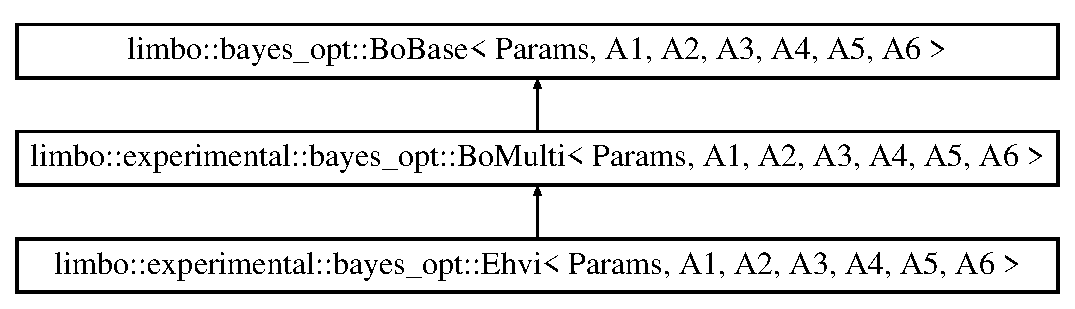
\includegraphics[height=3.000000cm]{classlimbo_1_1experimental_1_1bayes__opt_1_1_bo_multi}
\end{center}
\end{figure}
\subsection*{Public Types}
\begin{DoxyCompactItemize}
\item 
using \hyperlink{classlimbo_1_1experimental_1_1bayes__opt_1_1_bo_multi_a9ab4aaa59b6c7495da8e0220622efdea}{args} = typename bo\+\_\+multi\+\_\+signature\+::bind$<$ A1, A2, A3, A4, A5, A6 $>$\+::type
\item 
using \hyperlink{classlimbo_1_1experimental_1_1bayes__opt_1_1_bo_multi_a96e3df5190731faf8d60b20d6810ba64}{base\+\_\+t} = \hyperlink{classlimbo_1_1bayes__opt_1_1_bo_base}{limbo\+::bayes\+\_\+opt\+::\+Bo\+Base}$<$ Params, A1, A2, A3, A4, A5, A6 $>$
\item 
using \hyperlink{classlimbo_1_1experimental_1_1bayes__opt_1_1_bo_multi_abc4fa6ff00e1bf591283e5a2739fb6c8}{model\+\_\+t} = typename \hyperlink{classlimbo_1_1bayes__opt_1_1_bo_base_a5e23d523dd2a16b866a2660721b937bb}{base\+\_\+t\+::model\+\_\+t}
\item 
using \hyperlink{classlimbo_1_1experimental_1_1bayes__opt_1_1_bo_multi_aa9e161c2d3b75329a8470204c32f1458}{acquisition\+\_\+function\+\_\+t} = typename \hyperlink{classlimbo_1_1bayes__opt_1_1_bo_base_a5abe502b49e1ee70d5e00f27f95f5dff}{base\+\_\+t\+::acquisition\+\_\+function\+\_\+t}
\item 
using \hyperlink{classlimbo_1_1experimental_1_1bayes__opt_1_1_bo_multi_a5592d2f8141fec88904c0f60beb7ff2d}{pareto\+\_\+point\+\_\+t} = std\+::tuple$<$ Eigen\+::\+Vector\+Xd, Eigen\+::\+Vector\+Xd, Eigen\+::\+Vector\+Xd $>$
\item 
using \hyperlink{classlimbo_1_1experimental_1_1bayes__opt_1_1_bo_multi_aba7172aa379e749ea5cb85c8773e6408}{pareto\+\_\+t} = std\+::vector$<$ \hyperlink{classlimbo_1_1experimental_1_1bayes__opt_1_1_bo_multi_a5592d2f8141fec88904c0f60beb7ff2d}{pareto\+\_\+point\+\_\+t} $>$
\end{DoxyCompactItemize}
\subsection*{Public Member Functions}
\begin{DoxyCompactItemize}
\item 
size\+\_\+t \hyperlink{classlimbo_1_1experimental_1_1bayes__opt_1_1_bo_multi_a3817f6ffa5860e8530c663083dd0f9b0}{nb\+\_\+objs} () const 
\item 
const \hyperlink{classlimbo_1_1experimental_1_1bayes__opt_1_1_bo_multi_aba7172aa379e749ea5cb85c8773e6408}{pareto\+\_\+t} \& \hyperlink{classlimbo_1_1experimental_1_1bayes__opt_1_1_bo_multi_a74989812b92d1f938169d434906c1416}{pareto\+\_\+model} () const 
\item 
const \hyperlink{classlimbo_1_1experimental_1_1bayes__opt_1_1_bo_multi_aba7172aa379e749ea5cb85c8773e6408}{pareto\+\_\+t} \& \hyperlink{classlimbo_1_1experimental_1_1bayes__opt_1_1_bo_multi_a4572fa750cb3678783af45d89d026f9f}{pareto\+\_\+data} () const 
\item 
const std\+::vector$<$ \hyperlink{classlimbo_1_1experimental_1_1bayes__opt_1_1_bo_multi_abc4fa6ff00e1bf591283e5a2739fb6c8}{model\+\_\+t} $>$ \& \hyperlink{classlimbo_1_1experimental_1_1bayes__opt_1_1_bo_multi_a50114c72da6ef12f29938df0c8b0bcc6}{models} () const 
\item 
void \hyperlink{classlimbo_1_1experimental_1_1bayes__opt_1_1_bo_multi_a43c817f66221750175b905eab3640a19}{update\+\_\+pareto\+\_\+data} ()
\item 
{\footnotesize template$<$int D$>$ }\\void \hyperlink{classlimbo_1_1experimental_1_1bayes__opt_1_1_bo_multi_ad6240a53ed0faf0ed638f357aa99f31d}{update\+\_\+pareto\+\_\+model} ()
\end{DoxyCompactItemize}


\subsection{Member Typedef Documentation}
\hypertarget{classlimbo_1_1experimental_1_1bayes__opt_1_1_bo_multi_aa9e161c2d3b75329a8470204c32f1458}{}\index{limbo\+::experimental\+::bayes\+\_\+opt\+::\+Bo\+Multi@{limbo\+::experimental\+::bayes\+\_\+opt\+::\+Bo\+Multi}!acquisition\+\_\+function\+\_\+t@{acquisition\+\_\+function\+\_\+t}}
\index{acquisition\+\_\+function\+\_\+t@{acquisition\+\_\+function\+\_\+t}!limbo\+::experimental\+::bayes\+\_\+opt\+::\+Bo\+Multi@{limbo\+::experimental\+::bayes\+\_\+opt\+::\+Bo\+Multi}}
\subsubsection[{acquisition\+\_\+function\+\_\+t}]{\setlength{\rightskip}{0pt plus 5cm}template$<$class Params, class A1 = boost\+::parameter\+::void\+\_\+, class A2 = boost\+::parameter\+::void\+\_\+, class A3 = boost\+::parameter\+::void\+\_\+, class A4 = boost\+::parameter\+::void\+\_\+, class A5 = boost\+::parameter\+::void\+\_\+, class A6 = boost\+::parameter\+::void\+\_\+$>$ using {\bf limbo\+::experimental\+::bayes\+\_\+opt\+::\+Bo\+Multi}$<$ Params, A1, A2, A3, A4, A5, A6 $>$\+::{\bf acquisition\+\_\+function\+\_\+t} =  typename {\bf base\+\_\+t\+::acquisition\+\_\+function\+\_\+t}}\label{classlimbo_1_1experimental_1_1bayes__opt_1_1_bo_multi_aa9e161c2d3b75329a8470204c32f1458}
\hypertarget{classlimbo_1_1experimental_1_1bayes__opt_1_1_bo_multi_a9ab4aaa59b6c7495da8e0220622efdea}{}\index{limbo\+::experimental\+::bayes\+\_\+opt\+::\+Bo\+Multi@{limbo\+::experimental\+::bayes\+\_\+opt\+::\+Bo\+Multi}!args@{args}}
\index{args@{args}!limbo\+::experimental\+::bayes\+\_\+opt\+::\+Bo\+Multi@{limbo\+::experimental\+::bayes\+\_\+opt\+::\+Bo\+Multi}}
\subsubsection[{args}]{\setlength{\rightskip}{0pt plus 5cm}template$<$class Params, class A1 = boost\+::parameter\+::void\+\_\+, class A2 = boost\+::parameter\+::void\+\_\+, class A3 = boost\+::parameter\+::void\+\_\+, class A4 = boost\+::parameter\+::void\+\_\+, class A5 = boost\+::parameter\+::void\+\_\+, class A6 = boost\+::parameter\+::void\+\_\+$>$ using {\bf limbo\+::experimental\+::bayes\+\_\+opt\+::\+Bo\+Multi}$<$ Params, A1, A2, A3, A4, A5, A6 $>$\+::{\bf args} =  typename bo\+\_\+multi\+\_\+signature\+::bind$<$A1, A2, A3, A4, A5, A6$>$\+::type}\label{classlimbo_1_1experimental_1_1bayes__opt_1_1_bo_multi_a9ab4aaa59b6c7495da8e0220622efdea}
\hypertarget{classlimbo_1_1experimental_1_1bayes__opt_1_1_bo_multi_a96e3df5190731faf8d60b20d6810ba64}{}\index{limbo\+::experimental\+::bayes\+\_\+opt\+::\+Bo\+Multi@{limbo\+::experimental\+::bayes\+\_\+opt\+::\+Bo\+Multi}!base\+\_\+t@{base\+\_\+t}}
\index{base\+\_\+t@{base\+\_\+t}!limbo\+::experimental\+::bayes\+\_\+opt\+::\+Bo\+Multi@{limbo\+::experimental\+::bayes\+\_\+opt\+::\+Bo\+Multi}}
\subsubsection[{base\+\_\+t}]{\setlength{\rightskip}{0pt plus 5cm}template$<$class Params, class A1 = boost\+::parameter\+::void\+\_\+, class A2 = boost\+::parameter\+::void\+\_\+, class A3 = boost\+::parameter\+::void\+\_\+, class A4 = boost\+::parameter\+::void\+\_\+, class A5 = boost\+::parameter\+::void\+\_\+, class A6 = boost\+::parameter\+::void\+\_\+$>$ using {\bf limbo\+::experimental\+::bayes\+\_\+opt\+::\+Bo\+Multi}$<$ Params, A1, A2, A3, A4, A5, A6 $>$\+::{\bf base\+\_\+t} =  {\bf limbo\+::bayes\+\_\+opt\+::\+Bo\+Base}$<$Params, A1, A2, A3, A4, A5, A6$>$}\label{classlimbo_1_1experimental_1_1bayes__opt_1_1_bo_multi_a96e3df5190731faf8d60b20d6810ba64}
\hypertarget{classlimbo_1_1experimental_1_1bayes__opt_1_1_bo_multi_abc4fa6ff00e1bf591283e5a2739fb6c8}{}\index{limbo\+::experimental\+::bayes\+\_\+opt\+::\+Bo\+Multi@{limbo\+::experimental\+::bayes\+\_\+opt\+::\+Bo\+Multi}!model\+\_\+t@{model\+\_\+t}}
\index{model\+\_\+t@{model\+\_\+t}!limbo\+::experimental\+::bayes\+\_\+opt\+::\+Bo\+Multi@{limbo\+::experimental\+::bayes\+\_\+opt\+::\+Bo\+Multi}}
\subsubsection[{model\+\_\+t}]{\setlength{\rightskip}{0pt plus 5cm}template$<$class Params, class A1 = boost\+::parameter\+::void\+\_\+, class A2 = boost\+::parameter\+::void\+\_\+, class A3 = boost\+::parameter\+::void\+\_\+, class A4 = boost\+::parameter\+::void\+\_\+, class A5 = boost\+::parameter\+::void\+\_\+, class A6 = boost\+::parameter\+::void\+\_\+$>$ using {\bf limbo\+::experimental\+::bayes\+\_\+opt\+::\+Bo\+Multi}$<$ Params, A1, A2, A3, A4, A5, A6 $>$\+::{\bf model\+\_\+t} =  typename {\bf base\+\_\+t\+::model\+\_\+t}}\label{classlimbo_1_1experimental_1_1bayes__opt_1_1_bo_multi_abc4fa6ff00e1bf591283e5a2739fb6c8}
\hypertarget{classlimbo_1_1experimental_1_1bayes__opt_1_1_bo_multi_a5592d2f8141fec88904c0f60beb7ff2d}{}\index{limbo\+::experimental\+::bayes\+\_\+opt\+::\+Bo\+Multi@{limbo\+::experimental\+::bayes\+\_\+opt\+::\+Bo\+Multi}!pareto\+\_\+point\+\_\+t@{pareto\+\_\+point\+\_\+t}}
\index{pareto\+\_\+point\+\_\+t@{pareto\+\_\+point\+\_\+t}!limbo\+::experimental\+::bayes\+\_\+opt\+::\+Bo\+Multi@{limbo\+::experimental\+::bayes\+\_\+opt\+::\+Bo\+Multi}}
\subsubsection[{pareto\+\_\+point\+\_\+t}]{\setlength{\rightskip}{0pt plus 5cm}template$<$class Params, class A1 = boost\+::parameter\+::void\+\_\+, class A2 = boost\+::parameter\+::void\+\_\+, class A3 = boost\+::parameter\+::void\+\_\+, class A4 = boost\+::parameter\+::void\+\_\+, class A5 = boost\+::parameter\+::void\+\_\+, class A6 = boost\+::parameter\+::void\+\_\+$>$ using {\bf limbo\+::experimental\+::bayes\+\_\+opt\+::\+Bo\+Multi}$<$ Params, A1, A2, A3, A4, A5, A6 $>$\+::{\bf pareto\+\_\+point\+\_\+t} =  std\+::tuple$<$Eigen\+::\+Vector\+Xd, Eigen\+::\+Vector\+Xd, Eigen\+::\+Vector\+Xd$>$}\label{classlimbo_1_1experimental_1_1bayes__opt_1_1_bo_multi_a5592d2f8141fec88904c0f60beb7ff2d}
\hypertarget{classlimbo_1_1experimental_1_1bayes__opt_1_1_bo_multi_aba7172aa379e749ea5cb85c8773e6408}{}\index{limbo\+::experimental\+::bayes\+\_\+opt\+::\+Bo\+Multi@{limbo\+::experimental\+::bayes\+\_\+opt\+::\+Bo\+Multi}!pareto\+\_\+t@{pareto\+\_\+t}}
\index{pareto\+\_\+t@{pareto\+\_\+t}!limbo\+::experimental\+::bayes\+\_\+opt\+::\+Bo\+Multi@{limbo\+::experimental\+::bayes\+\_\+opt\+::\+Bo\+Multi}}
\subsubsection[{pareto\+\_\+t}]{\setlength{\rightskip}{0pt plus 5cm}template$<$class Params, class A1 = boost\+::parameter\+::void\+\_\+, class A2 = boost\+::parameter\+::void\+\_\+, class A3 = boost\+::parameter\+::void\+\_\+, class A4 = boost\+::parameter\+::void\+\_\+, class A5 = boost\+::parameter\+::void\+\_\+, class A6 = boost\+::parameter\+::void\+\_\+$>$ using {\bf limbo\+::experimental\+::bayes\+\_\+opt\+::\+Bo\+Multi}$<$ Params, A1, A2, A3, A4, A5, A6 $>$\+::{\bf pareto\+\_\+t} =  std\+::vector$<${\bf pareto\+\_\+point\+\_\+t}$>$}\label{classlimbo_1_1experimental_1_1bayes__opt_1_1_bo_multi_aba7172aa379e749ea5cb85c8773e6408}


\subsection{Member Function Documentation}
\hypertarget{classlimbo_1_1experimental_1_1bayes__opt_1_1_bo_multi_a50114c72da6ef12f29938df0c8b0bcc6}{}\index{limbo\+::experimental\+::bayes\+\_\+opt\+::\+Bo\+Multi@{limbo\+::experimental\+::bayes\+\_\+opt\+::\+Bo\+Multi}!models@{models}}
\index{models@{models}!limbo\+::experimental\+::bayes\+\_\+opt\+::\+Bo\+Multi@{limbo\+::experimental\+::bayes\+\_\+opt\+::\+Bo\+Multi}}
\subsubsection[{models}]{\setlength{\rightskip}{0pt plus 5cm}template$<$class Params, class A1 = boost\+::parameter\+::void\+\_\+, class A2 = boost\+::parameter\+::void\+\_\+, class A3 = boost\+::parameter\+::void\+\_\+, class A4 = boost\+::parameter\+::void\+\_\+, class A5 = boost\+::parameter\+::void\+\_\+, class A6 = boost\+::parameter\+::void\+\_\+$>$ const std\+::vector$<${\bf model\+\_\+t}$>$\& {\bf limbo\+::experimental\+::bayes\+\_\+opt\+::\+Bo\+Multi}$<$ Params, A1, A2, A3, A4, A5, A6 $>$\+::models (
\begin{DoxyParamCaption}
{}
\end{DoxyParamCaption}
) const\hspace{0.3cm}{\ttfamily [inline]}}\label{classlimbo_1_1experimental_1_1bayes__opt_1_1_bo_multi_a50114c72da6ef12f29938df0c8b0bcc6}
\hypertarget{classlimbo_1_1experimental_1_1bayes__opt_1_1_bo_multi_a3817f6ffa5860e8530c663083dd0f9b0}{}\index{limbo\+::experimental\+::bayes\+\_\+opt\+::\+Bo\+Multi@{limbo\+::experimental\+::bayes\+\_\+opt\+::\+Bo\+Multi}!nb\+\_\+objs@{nb\+\_\+objs}}
\index{nb\+\_\+objs@{nb\+\_\+objs}!limbo\+::experimental\+::bayes\+\_\+opt\+::\+Bo\+Multi@{limbo\+::experimental\+::bayes\+\_\+opt\+::\+Bo\+Multi}}
\subsubsection[{nb\+\_\+objs}]{\setlength{\rightskip}{0pt plus 5cm}template$<$class Params, class A1 = boost\+::parameter\+::void\+\_\+, class A2 = boost\+::parameter\+::void\+\_\+, class A3 = boost\+::parameter\+::void\+\_\+, class A4 = boost\+::parameter\+::void\+\_\+, class A5 = boost\+::parameter\+::void\+\_\+, class A6 = boost\+::parameter\+::void\+\_\+$>$ size\+\_\+t {\bf limbo\+::experimental\+::bayes\+\_\+opt\+::\+Bo\+Multi}$<$ Params, A1, A2, A3, A4, A5, A6 $>$\+::nb\+\_\+objs (
\begin{DoxyParamCaption}
{}
\end{DoxyParamCaption}
) const\hspace{0.3cm}{\ttfamily [inline]}}\label{classlimbo_1_1experimental_1_1bayes__opt_1_1_bo_multi_a3817f6ffa5860e8530c663083dd0f9b0}
\hypertarget{classlimbo_1_1experimental_1_1bayes__opt_1_1_bo_multi_a4572fa750cb3678783af45d89d026f9f}{}\index{limbo\+::experimental\+::bayes\+\_\+opt\+::\+Bo\+Multi@{limbo\+::experimental\+::bayes\+\_\+opt\+::\+Bo\+Multi}!pareto\+\_\+data@{pareto\+\_\+data}}
\index{pareto\+\_\+data@{pareto\+\_\+data}!limbo\+::experimental\+::bayes\+\_\+opt\+::\+Bo\+Multi@{limbo\+::experimental\+::bayes\+\_\+opt\+::\+Bo\+Multi}}
\subsubsection[{pareto\+\_\+data}]{\setlength{\rightskip}{0pt plus 5cm}template$<$class Params, class A1 = boost\+::parameter\+::void\+\_\+, class A2 = boost\+::parameter\+::void\+\_\+, class A3 = boost\+::parameter\+::void\+\_\+, class A4 = boost\+::parameter\+::void\+\_\+, class A5 = boost\+::parameter\+::void\+\_\+, class A6 = boost\+::parameter\+::void\+\_\+$>$ const {\bf pareto\+\_\+t}\& {\bf limbo\+::experimental\+::bayes\+\_\+opt\+::\+Bo\+Multi}$<$ Params, A1, A2, A3, A4, A5, A6 $>$\+::pareto\+\_\+data (
\begin{DoxyParamCaption}
{}
\end{DoxyParamCaption}
) const\hspace{0.3cm}{\ttfamily [inline]}}\label{classlimbo_1_1experimental_1_1bayes__opt_1_1_bo_multi_a4572fa750cb3678783af45d89d026f9f}
\hypertarget{classlimbo_1_1experimental_1_1bayes__opt_1_1_bo_multi_a74989812b92d1f938169d434906c1416}{}\index{limbo\+::experimental\+::bayes\+\_\+opt\+::\+Bo\+Multi@{limbo\+::experimental\+::bayes\+\_\+opt\+::\+Bo\+Multi}!pareto\+\_\+model@{pareto\+\_\+model}}
\index{pareto\+\_\+model@{pareto\+\_\+model}!limbo\+::experimental\+::bayes\+\_\+opt\+::\+Bo\+Multi@{limbo\+::experimental\+::bayes\+\_\+opt\+::\+Bo\+Multi}}
\subsubsection[{pareto\+\_\+model}]{\setlength{\rightskip}{0pt plus 5cm}template$<$class Params, class A1 = boost\+::parameter\+::void\+\_\+, class A2 = boost\+::parameter\+::void\+\_\+, class A3 = boost\+::parameter\+::void\+\_\+, class A4 = boost\+::parameter\+::void\+\_\+, class A5 = boost\+::parameter\+::void\+\_\+, class A6 = boost\+::parameter\+::void\+\_\+$>$ const {\bf pareto\+\_\+t}\& {\bf limbo\+::experimental\+::bayes\+\_\+opt\+::\+Bo\+Multi}$<$ Params, A1, A2, A3, A4, A5, A6 $>$\+::pareto\+\_\+model (
\begin{DoxyParamCaption}
{}
\end{DoxyParamCaption}
) const\hspace{0.3cm}{\ttfamily [inline]}}\label{classlimbo_1_1experimental_1_1bayes__opt_1_1_bo_multi_a74989812b92d1f938169d434906c1416}
\hypertarget{classlimbo_1_1experimental_1_1bayes__opt_1_1_bo_multi_a43c817f66221750175b905eab3640a19}{}\index{limbo\+::experimental\+::bayes\+\_\+opt\+::\+Bo\+Multi@{limbo\+::experimental\+::bayes\+\_\+opt\+::\+Bo\+Multi}!update\+\_\+pareto\+\_\+data@{update\+\_\+pareto\+\_\+data}}
\index{update\+\_\+pareto\+\_\+data@{update\+\_\+pareto\+\_\+data}!limbo\+::experimental\+::bayes\+\_\+opt\+::\+Bo\+Multi@{limbo\+::experimental\+::bayes\+\_\+opt\+::\+Bo\+Multi}}
\subsubsection[{update\+\_\+pareto\+\_\+data}]{\setlength{\rightskip}{0pt plus 5cm}template$<$class Params, class A1 = boost\+::parameter\+::void\+\_\+, class A2 = boost\+::parameter\+::void\+\_\+, class A3 = boost\+::parameter\+::void\+\_\+, class A4 = boost\+::parameter\+::void\+\_\+, class A5 = boost\+::parameter\+::void\+\_\+, class A6 = boost\+::parameter\+::void\+\_\+$>$ void {\bf limbo\+::experimental\+::bayes\+\_\+opt\+::\+Bo\+Multi}$<$ Params, A1, A2, A3, A4, A5, A6 $>$\+::update\+\_\+pareto\+\_\+data (
\begin{DoxyParamCaption}
{}
\end{DoxyParamCaption}
)\hspace{0.3cm}{\ttfamily [inline]}}\label{classlimbo_1_1experimental_1_1bayes__opt_1_1_bo_multi_a43c817f66221750175b905eab3640a19}
\hypertarget{classlimbo_1_1experimental_1_1bayes__opt_1_1_bo_multi_ad6240a53ed0faf0ed638f357aa99f31d}{}\index{limbo\+::experimental\+::bayes\+\_\+opt\+::\+Bo\+Multi@{limbo\+::experimental\+::bayes\+\_\+opt\+::\+Bo\+Multi}!update\+\_\+pareto\+\_\+model@{update\+\_\+pareto\+\_\+model}}
\index{update\+\_\+pareto\+\_\+model@{update\+\_\+pareto\+\_\+model}!limbo\+::experimental\+::bayes\+\_\+opt\+::\+Bo\+Multi@{limbo\+::experimental\+::bayes\+\_\+opt\+::\+Bo\+Multi}}
\subsubsection[{update\+\_\+pareto\+\_\+model}]{\setlength{\rightskip}{0pt plus 5cm}template$<$class Params, class A1 = boost\+::parameter\+::void\+\_\+, class A2 = boost\+::parameter\+::void\+\_\+, class A3 = boost\+::parameter\+::void\+\_\+, class A4 = boost\+::parameter\+::void\+\_\+, class A5 = boost\+::parameter\+::void\+\_\+, class A6 = boost\+::parameter\+::void\+\_\+$>$ template$<$int D$>$ void {\bf limbo\+::experimental\+::bayes\+\_\+opt\+::\+Bo\+Multi}$<$ Params, A1, A2, A3, A4, A5, A6 $>$\+::update\+\_\+pareto\+\_\+model (
\begin{DoxyParamCaption}
{}
\end{DoxyParamCaption}
)\hspace{0.3cm}{\ttfamily [inline]}}\label{classlimbo_1_1experimental_1_1bayes__opt_1_1_bo_multi_ad6240a53ed0faf0ed638f357aa99f31d}


The documentation for this class was generated from the following file\+:\begin{DoxyCompactItemize}
\item 
/tmp/doc\+\_\+limbo/limbo/src/limbo/experimental/bayes\+\_\+opt/\hyperlink{bo__multi_8hpp}{bo\+\_\+multi.\+hpp}\end{DoxyCompactItemize}

\hypertarget{classlimbo_1_1bayes__opt_1_1_b_optimizer}{}\section{limbo\+:\+:bayes\+\_\+opt\+:\+:B\+Optimizer$<$ Params, A1, A2, A3, A4, A5, A6 $>$ Class Template Reference}
\label{classlimbo_1_1bayes__opt_1_1_b_optimizer}\index{limbo\+::bayes\+\_\+opt\+::\+B\+Optimizer$<$ Params, A1, A2, A3, A4, A5, A6 $>$@{limbo\+::bayes\+\_\+opt\+::\+B\+Optimizer$<$ Params, A1, A2, A3, A4, A5, A6 $>$}}


{\ttfamily \#include $<$limbo/bayes\+\_\+opt/boptimizer.\+hpp$>$}

Inheritance diagram for limbo\+:\+:bayes\+\_\+opt\+:\+:B\+Optimizer$<$ Params, A1, A2, A3, A4, A5, A6 $>$\+:\begin{figure}[H]
\begin{center}
\leavevmode
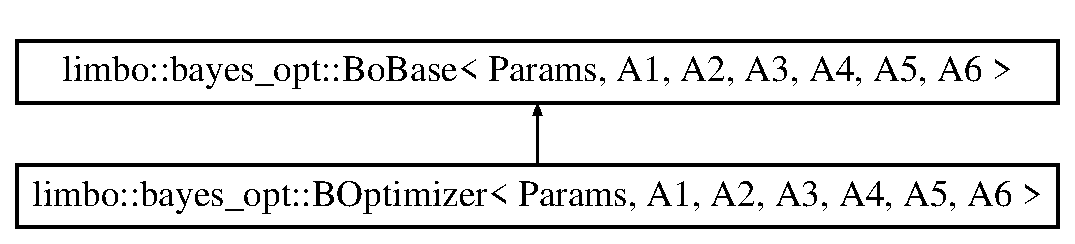
\includegraphics[height=2.000000cm]{classlimbo_1_1bayes__opt_1_1_b_optimizer}
\end{center}
\end{figure}
\subsection*{Classes}
\begin{DoxyCompactItemize}
\item 
struct \hyperlink{structlimbo_1_1bayes__opt_1_1_b_optimizer_1_1defaults}{defaults}
\end{DoxyCompactItemize}
\subsection*{Public Types}
\begin{DoxyCompactItemize}
\item 
typedef \hyperlink{classlimbo_1_1bayes__opt_1_1_bo_base}{Bo\+Base}$<$ Params, A1, A2, A3, A4, A5 $>$ \hyperlink{classlimbo_1_1bayes__opt_1_1_b_optimizer_a89d1cce7fdecc3598db103e337d942de}{base\+\_\+t}
\begin{DoxyCompactList}\small\item\em link to the corresponding \hyperlink{classlimbo_1_1bayes__opt_1_1_bo_base}{Bo\+Base} (useful for typedefs) \end{DoxyCompactList}\item 
typedef \hyperlink{classlimbo_1_1bayes__opt_1_1_bo_base_a1ddc93cc023a2d7d527deb4cc750624e}{base\+\_\+t\+::model\+\_\+t} \hyperlink{classlimbo_1_1bayes__opt_1_1_b_optimizer_aaddb85f5014ba377c9e2e3a64db87678}{model\+\_\+t}
\item 
typedef \hyperlink{classlimbo_1_1bayes__opt_1_1_bo_base_a02b14991b62e0f8c9bcf834220ed62e4}{base\+\_\+t\+::acquisition\+\_\+function\+\_\+t} \hyperlink{classlimbo_1_1bayes__opt_1_1_b_optimizer_ae0a407a5eba370a6a30acda501cd4ddc}{acquisition\+\_\+function\+\_\+t}
\item 
typedef boptimizer\+\_\+signature\+::bind$<$ A1, A2, A3, A4, A5, A6 $>$\+::type \hyperlink{classlimbo_1_1bayes__opt_1_1_b_optimizer_afd4c6a7d361de59fac5aa3a332ea0149}{args}
\item 
typedef boost\+::parameter\+::binding$<$ \hyperlink{classlimbo_1_1bayes__opt_1_1_bo_base_a75c1ae9e7268016c6f767c56bcede7d2}{args}, tag\+::acquiopt, typename \hyperlink{structlimbo_1_1bayes__opt_1_1_b_optimizer_1_1defaults_a4eb44d2abad01f5ef0206b7c5c595c7b}{defaults\+::acquiopt\+\_\+t} $>$\+::type \hyperlink{classlimbo_1_1bayes__opt_1_1_b_optimizer_a18dc1b593c859b8f89450a31f80fb592}{acqui\+\_\+optimizer\+\_\+t}
\end{DoxyCompactItemize}
\subsection*{Public Member Functions}
\begin{DoxyCompactItemize}
\item 
{\footnotesize template$<$typename State\+Function , typename Aggregator\+Function  = First\+Elem$>$ }\\void \hyperlink{classlimbo_1_1bayes__opt_1_1_b_optimizer_a731de253fe21749b9a00e609aae0386f}{optimize} (const State\+Function \&sfun, const Aggregator\+Function \&afun=Aggregator\+Function(), bool reset=true)
\begin{DoxyCompactList}\small\item\em The main function (run the Bayesian optimization algorithm) \end{DoxyCompactList}\item 
{\footnotesize template$<$typename Aggregator\+Function  = First\+Elem$>$ }\\const Eigen\+::\+Vector\+Xd \& \hyperlink{classlimbo_1_1bayes__opt_1_1_b_optimizer_aac35dbb6504e5a1b7d5fc9252c5e6a51}{best\+\_\+observation} (const Aggregator\+Function \&afun=Aggregator\+Function()) const 
\begin{DoxyCompactList}\small\item\em return the best observation so far (i.\+e. max(f(x))) \end{DoxyCompactList}\item 
{\footnotesize template$<$typename Aggregator\+Function  = First\+Elem$>$ }\\const Eigen\+::\+Vector\+Xd \& \hyperlink{classlimbo_1_1bayes__opt_1_1_b_optimizer_ad3a19271e9d00827648f83b0dccc66b0}{best\+\_\+sample} (const Aggregator\+Function \&afun=Aggregator\+Function()) const 
\begin{DoxyCompactList}\small\item\em return the best sample so far (i.\+e. the argmax(f(x))) \end{DoxyCompactList}\item 
const \hyperlink{classlimbo_1_1bayes__opt_1_1_bo_base_a1ddc93cc023a2d7d527deb4cc750624e}{model\+\_\+t} \& \hyperlink{classlimbo_1_1bayes__opt_1_1_b_optimizer_a1f338242d56d6a2b97245ca3bcaf991f}{model} () const 
\end{DoxyCompactItemize}


\subsection{Detailed Description}
\subsubsection*{template$<$class Params, class A1 = boost\+::parameter\+::void\+\_\+, class A2 = boost\+::parameter\+::void\+\_\+, class A3 = boost\+::parameter\+::void\+\_\+, class A4 = boost\+::parameter\+::void\+\_\+, class A5 = boost\+::parameter\+::void\+\_\+, class A6 = boost\+::parameter\+::void\+\_\+$>$class limbo\+::bayes\+\_\+opt\+::\+B\+Optimizer$<$ Params, A1, A2, A3, A4, A5, A6 $>$}

The classic Bayesian optimization algorithm.

\begin{DoxyVerb}embed:rst
References: :cite:`brochu2010tutorial,Mockus2013`
\end{DoxyVerb}


This class takes the same template parameters as \hyperlink{classlimbo_1_1bayes__opt_1_1_bo_base}{Bo\+Base}. It adds\+: \begin{DoxyVerb}embed:rst
+---------------------+------------+----------+---------------+
|type                 |typedef     | argument | default       |
+=====================+============+==========+===============+
|acqui. optimizer     |acqui_opt_t | acquiopt | see below     |
+---------------------+------------+----------+---------------+
\end{DoxyVerb}


The default value of acqui\+\_\+opt\+\_\+t is\+:
\begin{DoxyItemize}
\item {\ttfamily \hyperlink{structlimbo_1_1opt_1_1_cmaes}{opt\+::\+Cmaes}$<$Params$>$} if libcmaes was found in {\ttfamily waf configure}
\item {\ttfamily \hyperlink{structlimbo_1_1opt_1_1_n_l_opt_no_grad}{opt\+::\+N\+L\+Opt\+No\+Grad}$<$Params, nlopt\+::\+G\+N\+\_\+\+D\+I\+R\+E\+C\+T\+\_\+\+L\+\_\+\+R\+A\+N\+D$>$} if N\+L\+Opt was found but libcmaes was not found
\item {\ttfamily \hyperlink{structlimbo_1_1opt_1_1_grid_search}{opt\+::\+Grid\+Search}$<$Params$>$} otherwise (please do not use this\+: the algorithm will not work at all!) 
\end{DoxyItemize}

\subsection{Member Typedef Documentation}
\hypertarget{classlimbo_1_1bayes__opt_1_1_b_optimizer_a18dc1b593c859b8f89450a31f80fb592}{}\index{limbo\+::bayes\+\_\+opt\+::\+B\+Optimizer@{limbo\+::bayes\+\_\+opt\+::\+B\+Optimizer}!acqui\+\_\+optimizer\+\_\+t@{acqui\+\_\+optimizer\+\_\+t}}
\index{acqui\+\_\+optimizer\+\_\+t@{acqui\+\_\+optimizer\+\_\+t}!limbo\+::bayes\+\_\+opt\+::\+B\+Optimizer@{limbo\+::bayes\+\_\+opt\+::\+B\+Optimizer}}
\subsubsection[{acqui\+\_\+optimizer\+\_\+t}]{\setlength{\rightskip}{0pt plus 5cm}template$<$class Params, class A1 = boost\+::parameter\+::void\+\_\+, class A2 = boost\+::parameter\+::void\+\_\+, class A3 = boost\+::parameter\+::void\+\_\+, class A4 = boost\+::parameter\+::void\+\_\+, class A5 = boost\+::parameter\+::void\+\_\+, class A6 = boost\+::parameter\+::void\+\_\+$>$ typedef boost\+::parameter\+::binding$<${\bf args}, tag\+::acquiopt, typename {\bf defaults\+::acquiopt\+\_\+t}$>$\+::type {\bf limbo\+::bayes\+\_\+opt\+::\+B\+Optimizer}$<$ Params, A1, A2, A3, A4, A5, A6 $>$\+::{\bf acqui\+\_\+optimizer\+\_\+t}}\label{classlimbo_1_1bayes__opt_1_1_b_optimizer_a18dc1b593c859b8f89450a31f80fb592}
\hypertarget{classlimbo_1_1bayes__opt_1_1_b_optimizer_ae0a407a5eba370a6a30acda501cd4ddc}{}\index{limbo\+::bayes\+\_\+opt\+::\+B\+Optimizer@{limbo\+::bayes\+\_\+opt\+::\+B\+Optimizer}!acquisition\+\_\+function\+\_\+t@{acquisition\+\_\+function\+\_\+t}}
\index{acquisition\+\_\+function\+\_\+t@{acquisition\+\_\+function\+\_\+t}!limbo\+::bayes\+\_\+opt\+::\+B\+Optimizer@{limbo\+::bayes\+\_\+opt\+::\+B\+Optimizer}}
\subsubsection[{acquisition\+\_\+function\+\_\+t}]{\setlength{\rightskip}{0pt plus 5cm}template$<$class Params, class A1 = boost\+::parameter\+::void\+\_\+, class A2 = boost\+::parameter\+::void\+\_\+, class A3 = boost\+::parameter\+::void\+\_\+, class A4 = boost\+::parameter\+::void\+\_\+, class A5 = boost\+::parameter\+::void\+\_\+, class A6 = boost\+::parameter\+::void\+\_\+$>$ typedef {\bf base\+\_\+t\+::acquisition\+\_\+function\+\_\+t} {\bf limbo\+::bayes\+\_\+opt\+::\+B\+Optimizer}$<$ Params, A1, A2, A3, A4, A5, A6 $>$\+::{\bf acquisition\+\_\+function\+\_\+t}}\label{classlimbo_1_1bayes__opt_1_1_b_optimizer_ae0a407a5eba370a6a30acda501cd4ddc}
\hypertarget{classlimbo_1_1bayes__opt_1_1_b_optimizer_afd4c6a7d361de59fac5aa3a332ea0149}{}\index{limbo\+::bayes\+\_\+opt\+::\+B\+Optimizer@{limbo\+::bayes\+\_\+opt\+::\+B\+Optimizer}!args@{args}}
\index{args@{args}!limbo\+::bayes\+\_\+opt\+::\+B\+Optimizer@{limbo\+::bayes\+\_\+opt\+::\+B\+Optimizer}}
\subsubsection[{args}]{\setlength{\rightskip}{0pt plus 5cm}template$<$class Params, class A1 = boost\+::parameter\+::void\+\_\+, class A2 = boost\+::parameter\+::void\+\_\+, class A3 = boost\+::parameter\+::void\+\_\+, class A4 = boost\+::parameter\+::void\+\_\+, class A5 = boost\+::parameter\+::void\+\_\+, class A6 = boost\+::parameter\+::void\+\_\+$>$ typedef boptimizer\+\_\+signature\+::bind$<$A1, A2, A3, A4, A5, A6$>$\+::type {\bf limbo\+::bayes\+\_\+opt\+::\+B\+Optimizer}$<$ Params, A1, A2, A3, A4, A5, A6 $>$\+::{\bf args}}\label{classlimbo_1_1bayes__opt_1_1_b_optimizer_afd4c6a7d361de59fac5aa3a332ea0149}
\hypertarget{classlimbo_1_1bayes__opt_1_1_b_optimizer_a89d1cce7fdecc3598db103e337d942de}{}\index{limbo\+::bayes\+\_\+opt\+::\+B\+Optimizer@{limbo\+::bayes\+\_\+opt\+::\+B\+Optimizer}!base\+\_\+t@{base\+\_\+t}}
\index{base\+\_\+t@{base\+\_\+t}!limbo\+::bayes\+\_\+opt\+::\+B\+Optimizer@{limbo\+::bayes\+\_\+opt\+::\+B\+Optimizer}}
\subsubsection[{base\+\_\+t}]{\setlength{\rightskip}{0pt plus 5cm}template$<$class Params, class A1 = boost\+::parameter\+::void\+\_\+, class A2 = boost\+::parameter\+::void\+\_\+, class A3 = boost\+::parameter\+::void\+\_\+, class A4 = boost\+::parameter\+::void\+\_\+, class A5 = boost\+::parameter\+::void\+\_\+, class A6 = boost\+::parameter\+::void\+\_\+$>$ typedef {\bf Bo\+Base}$<$Params, A1, A2, A3, A4, A5$>$ {\bf limbo\+::bayes\+\_\+opt\+::\+B\+Optimizer}$<$ Params, A1, A2, A3, A4, A5, A6 $>$\+::{\bf base\+\_\+t}}\label{classlimbo_1_1bayes__opt_1_1_b_optimizer_a89d1cce7fdecc3598db103e337d942de}


link to the corresponding \hyperlink{classlimbo_1_1bayes__opt_1_1_bo_base}{Bo\+Base} (useful for typedefs) 

\hypertarget{classlimbo_1_1bayes__opt_1_1_b_optimizer_aaddb85f5014ba377c9e2e3a64db87678}{}\index{limbo\+::bayes\+\_\+opt\+::\+B\+Optimizer@{limbo\+::bayes\+\_\+opt\+::\+B\+Optimizer}!model\+\_\+t@{model\+\_\+t}}
\index{model\+\_\+t@{model\+\_\+t}!limbo\+::bayes\+\_\+opt\+::\+B\+Optimizer@{limbo\+::bayes\+\_\+opt\+::\+B\+Optimizer}}
\subsubsection[{model\+\_\+t}]{\setlength{\rightskip}{0pt plus 5cm}template$<$class Params, class A1 = boost\+::parameter\+::void\+\_\+, class A2 = boost\+::parameter\+::void\+\_\+, class A3 = boost\+::parameter\+::void\+\_\+, class A4 = boost\+::parameter\+::void\+\_\+, class A5 = boost\+::parameter\+::void\+\_\+, class A6 = boost\+::parameter\+::void\+\_\+$>$ typedef {\bf base\+\_\+t\+::model\+\_\+t} {\bf limbo\+::bayes\+\_\+opt\+::\+B\+Optimizer}$<$ Params, A1, A2, A3, A4, A5, A6 $>$\+::{\bf model\+\_\+t}}\label{classlimbo_1_1bayes__opt_1_1_b_optimizer_aaddb85f5014ba377c9e2e3a64db87678}


\subsection{Member Function Documentation}
\hypertarget{classlimbo_1_1bayes__opt_1_1_b_optimizer_aac35dbb6504e5a1b7d5fc9252c5e6a51}{}\index{limbo\+::bayes\+\_\+opt\+::\+B\+Optimizer@{limbo\+::bayes\+\_\+opt\+::\+B\+Optimizer}!best\+\_\+observation@{best\+\_\+observation}}
\index{best\+\_\+observation@{best\+\_\+observation}!limbo\+::bayes\+\_\+opt\+::\+B\+Optimizer@{limbo\+::bayes\+\_\+opt\+::\+B\+Optimizer}}
\subsubsection[{best\+\_\+observation}]{\setlength{\rightskip}{0pt plus 5cm}template$<$class Params, class A1 = boost\+::parameter\+::void\+\_\+, class A2 = boost\+::parameter\+::void\+\_\+, class A3 = boost\+::parameter\+::void\+\_\+, class A4 = boost\+::parameter\+::void\+\_\+, class A5 = boost\+::parameter\+::void\+\_\+, class A6 = boost\+::parameter\+::void\+\_\+$>$ template$<$typename Aggregator\+Function  = First\+Elem$>$ const Eigen\+::\+Vector\+Xd\& {\bf limbo\+::bayes\+\_\+opt\+::\+B\+Optimizer}$<$ Params, A1, A2, A3, A4, A5, A6 $>$\+::best\+\_\+observation (
\begin{DoxyParamCaption}
\item[{const Aggregator\+Function \&}]{afun = {\ttfamily AggregatorFunction()}}
\end{DoxyParamCaption}
) const\hspace{0.3cm}{\ttfamily [inline]}}\label{classlimbo_1_1bayes__opt_1_1_b_optimizer_aac35dbb6504e5a1b7d5fc9252c5e6a51}


return the best observation so far (i.\+e. max(f(x))) 

\hypertarget{classlimbo_1_1bayes__opt_1_1_b_optimizer_ad3a19271e9d00827648f83b0dccc66b0}{}\index{limbo\+::bayes\+\_\+opt\+::\+B\+Optimizer@{limbo\+::bayes\+\_\+opt\+::\+B\+Optimizer}!best\+\_\+sample@{best\+\_\+sample}}
\index{best\+\_\+sample@{best\+\_\+sample}!limbo\+::bayes\+\_\+opt\+::\+B\+Optimizer@{limbo\+::bayes\+\_\+opt\+::\+B\+Optimizer}}
\subsubsection[{best\+\_\+sample}]{\setlength{\rightskip}{0pt plus 5cm}template$<$class Params, class A1 = boost\+::parameter\+::void\+\_\+, class A2 = boost\+::parameter\+::void\+\_\+, class A3 = boost\+::parameter\+::void\+\_\+, class A4 = boost\+::parameter\+::void\+\_\+, class A5 = boost\+::parameter\+::void\+\_\+, class A6 = boost\+::parameter\+::void\+\_\+$>$ template$<$typename Aggregator\+Function  = First\+Elem$>$ const Eigen\+::\+Vector\+Xd\& {\bf limbo\+::bayes\+\_\+opt\+::\+B\+Optimizer}$<$ Params, A1, A2, A3, A4, A5, A6 $>$\+::best\+\_\+sample (
\begin{DoxyParamCaption}
\item[{const Aggregator\+Function \&}]{afun = {\ttfamily AggregatorFunction()}}
\end{DoxyParamCaption}
) const\hspace{0.3cm}{\ttfamily [inline]}}\label{classlimbo_1_1bayes__opt_1_1_b_optimizer_ad3a19271e9d00827648f83b0dccc66b0}


return the best sample so far (i.\+e. the argmax(f(x))) 

\hypertarget{classlimbo_1_1bayes__opt_1_1_b_optimizer_a1f338242d56d6a2b97245ca3bcaf991f}{}\index{limbo\+::bayes\+\_\+opt\+::\+B\+Optimizer@{limbo\+::bayes\+\_\+opt\+::\+B\+Optimizer}!model@{model}}
\index{model@{model}!limbo\+::bayes\+\_\+opt\+::\+B\+Optimizer@{limbo\+::bayes\+\_\+opt\+::\+B\+Optimizer}}
\subsubsection[{model}]{\setlength{\rightskip}{0pt plus 5cm}template$<$class Params, class A1 = boost\+::parameter\+::void\+\_\+, class A2 = boost\+::parameter\+::void\+\_\+, class A3 = boost\+::parameter\+::void\+\_\+, class A4 = boost\+::parameter\+::void\+\_\+, class A5 = boost\+::parameter\+::void\+\_\+, class A6 = boost\+::parameter\+::void\+\_\+$>$ const {\bf model\+\_\+t}\& {\bf limbo\+::bayes\+\_\+opt\+::\+B\+Optimizer}$<$ Params, A1, A2, A3, A4, A5, A6 $>$\+::model (
\begin{DoxyParamCaption}
{}
\end{DoxyParamCaption}
) const\hspace{0.3cm}{\ttfamily [inline]}}\label{classlimbo_1_1bayes__opt_1_1_b_optimizer_a1f338242d56d6a2b97245ca3bcaf991f}
\hypertarget{classlimbo_1_1bayes__opt_1_1_b_optimizer_a731de253fe21749b9a00e609aae0386f}{}\index{limbo\+::bayes\+\_\+opt\+::\+B\+Optimizer@{limbo\+::bayes\+\_\+opt\+::\+B\+Optimizer}!optimize@{optimize}}
\index{optimize@{optimize}!limbo\+::bayes\+\_\+opt\+::\+B\+Optimizer@{limbo\+::bayes\+\_\+opt\+::\+B\+Optimizer}}
\subsubsection[{optimize}]{\setlength{\rightskip}{0pt plus 5cm}template$<$class Params, class A1 = boost\+::parameter\+::void\+\_\+, class A2 = boost\+::parameter\+::void\+\_\+, class A3 = boost\+::parameter\+::void\+\_\+, class A4 = boost\+::parameter\+::void\+\_\+, class A5 = boost\+::parameter\+::void\+\_\+, class A6 = boost\+::parameter\+::void\+\_\+$>$ template$<$typename State\+Function , typename Aggregator\+Function  = First\+Elem$>$ void {\bf limbo\+::bayes\+\_\+opt\+::\+B\+Optimizer}$<$ Params, A1, A2, A3, A4, A5, A6 $>$\+::optimize (
\begin{DoxyParamCaption}
\item[{const State\+Function \&}]{sfun, }
\item[{const Aggregator\+Function \&}]{afun = {\ttfamily AggregatorFunction()}, }
\item[{bool}]{reset = {\ttfamily true}}
\end{DoxyParamCaption}
)\hspace{0.3cm}{\ttfamily [inline]}}\label{classlimbo_1_1bayes__opt_1_1_b_optimizer_a731de253fe21749b9a00e609aae0386f}


The main function (run the Bayesian optimization algorithm) 



The documentation for this class was generated from the following file\+:\begin{DoxyCompactItemize}
\item 
/tmp/doc\+\_\+limbo/limbo/src/limbo/bayes\+\_\+opt/\hyperlink{boptimizer_8hpp}{boptimizer.\+hpp}\end{DoxyCompactItemize}

\hypertarget{structlimbo_1_1stop_1_1_chain_criteria}{}\section{limbo\+:\+:stop\+:\+:Chain\+Criteria$<$ BO, Aggregator\+Function $>$ Struct Template Reference}
\label{structlimbo_1_1stop_1_1_chain_criteria}\index{limbo\+::stop\+::\+Chain\+Criteria$<$ B\+O, Aggregator\+Function $>$@{limbo\+::stop\+::\+Chain\+Criteria$<$ B\+O, Aggregator\+Function $>$}}


{\ttfamily \#include $<$limbo/stop/chain\+\_\+criteria.\+hpp$>$}

\subsection*{Public Types}
\begin{DoxyCompactItemize}
\item 
using \hyperlink{structlimbo_1_1stop_1_1_chain_criteria_a3e9b4e7191e4568a44bba75647bf0fb5}{result\+\_\+type} = bool
\end{DoxyCompactItemize}
\subsection*{Public Member Functions}
\begin{DoxyCompactItemize}
\item 
\hyperlink{structlimbo_1_1stop_1_1_chain_criteria_a287a286866f5ddc83432f23dc1c7c63d}{Chain\+Criteria} (const BO \&bo, const Aggregator\+Function \&afun)
\item 
{\footnotesize template$<$typename stopping\+\_\+criterion $>$ }\\bool \hyperlink{structlimbo_1_1stop_1_1_chain_criteria_a1d95f89ebcc61121482a372d37c3a62f}{operator()} (bool state, stopping\+\_\+criterion stop) const 
\end{DoxyCompactItemize}


\subsection{Detailed Description}
\subsubsection*{template$<$typename BO, typename Aggregator\+Function$>$\\*
struct limbo\+::stop\+::\+Chain\+Criteria$<$ B\+O, Aggregator\+Function $>$}

\begin{DoxyVerb}embed:rst
Utility functor for boost::fusion::accumulate, e.g.:

.. code-block:: cpp

  stop::ChainCriteria<BO, AggregatorFunction> chain(bo, afun);
  return boost::fusion::accumulate(_stopping_criteria, false, chain);

Where ``_stopping_criteria` is a ``boost::fusion::vector`` of classes.\end{DoxyVerb}
 

\subsection{Member Typedef Documentation}
\index{limbo\+::stop\+::\+Chain\+Criteria@{limbo\+::stop\+::\+Chain\+Criteria}!result\+\_\+type@{result\+\_\+type}}
\index{result\+\_\+type@{result\+\_\+type}!limbo\+::stop\+::\+Chain\+Criteria@{limbo\+::stop\+::\+Chain\+Criteria}}
\subsubsection[{\texorpdfstring{result\+\_\+type}{result_type}}]{\setlength{\rightskip}{0pt plus 5cm}template$<$typename BO, typename Aggregator\+Function$>$ using {\bf limbo\+::stop\+::\+Chain\+Criteria}$<$ BO, Aggregator\+Function $>$\+::{\bf result\+\_\+type} =  bool}\hypertarget{structlimbo_1_1stop_1_1_chain_criteria_a3e9b4e7191e4568a44bba75647bf0fb5}{}\label{structlimbo_1_1stop_1_1_chain_criteria_a3e9b4e7191e4568a44bba75647bf0fb5}


\subsection{Constructor \& Destructor Documentation}
\index{limbo\+::stop\+::\+Chain\+Criteria@{limbo\+::stop\+::\+Chain\+Criteria}!Chain\+Criteria@{Chain\+Criteria}}
\index{Chain\+Criteria@{Chain\+Criteria}!limbo\+::stop\+::\+Chain\+Criteria@{limbo\+::stop\+::\+Chain\+Criteria}}
\subsubsection[{\texorpdfstring{Chain\+Criteria(const B\+O \&bo, const Aggregator\+Function \&afun)}{ChainCriteria(const BO &bo, const AggregatorFunction &afun)}}]{\setlength{\rightskip}{0pt plus 5cm}template$<$typename BO, typename Aggregator\+Function$>$ {\bf limbo\+::stop\+::\+Chain\+Criteria}$<$ BO, Aggregator\+Function $>$\+::{\bf Chain\+Criteria} (
\begin{DoxyParamCaption}
\item[{const BO \&}]{bo, }
\item[{const Aggregator\+Function \&}]{afun}
\end{DoxyParamCaption}
)\hspace{0.3cm}{\ttfamily [inline]}}\hypertarget{structlimbo_1_1stop_1_1_chain_criteria_a287a286866f5ddc83432f23dc1c7c63d}{}\label{structlimbo_1_1stop_1_1_chain_criteria_a287a286866f5ddc83432f23dc1c7c63d}


\subsection{Member Function Documentation}
\index{limbo\+::stop\+::\+Chain\+Criteria@{limbo\+::stop\+::\+Chain\+Criteria}!operator()@{operator()}}
\index{operator()@{operator()}!limbo\+::stop\+::\+Chain\+Criteria@{limbo\+::stop\+::\+Chain\+Criteria}}
\subsubsection[{\texorpdfstring{operator()(bool state, stopping\+\_\+criterion stop) const }{operator()(bool state, stopping_criterion stop) const }}]{\setlength{\rightskip}{0pt plus 5cm}template$<$typename BO, typename Aggregator\+Function$>$ template$<$typename stopping\+\_\+criterion $>$ bool {\bf limbo\+::stop\+::\+Chain\+Criteria}$<$ BO, Aggregator\+Function $>$\+::operator() (
\begin{DoxyParamCaption}
\item[{bool}]{state, }
\item[{stopping\+\_\+criterion}]{stop}
\end{DoxyParamCaption}
) const\hspace{0.3cm}{\ttfamily [inline]}}\hypertarget{structlimbo_1_1stop_1_1_chain_criteria_a1d95f89ebcc61121482a372d37c3a62f}{}\label{structlimbo_1_1stop_1_1_chain_criteria_a1d95f89ebcc61121482a372d37c3a62f}


The documentation for this struct was generated from the following file\+:\begin{DoxyCompactItemize}
\item 
/tmp/doc\+\_\+limbo/limbo/src/limbo/stop/\hyperlink{chain__criteria_8hpp}{chain\+\_\+criteria.\+hpp}\end{DoxyCompactItemize}

\hypertarget{structlimbo_1_1opt_1_1_chained}{}\section{limbo\+:\+:opt\+:\+:Chained$<$ Params, Optimizers $>$ Struct Template Reference}
\label{structlimbo_1_1opt_1_1_chained}\index{limbo\+::opt\+::\+Chained$<$ Params, Optimizers $>$@{limbo\+::opt\+::\+Chained$<$ Params, Optimizers $>$}}


{\ttfamily \#include $<$limbo/opt/chained.\+hpp$>$}



The documentation for this struct was generated from the following file\+:\begin{DoxyCompactItemize}
\item 
/tmp/doc\+\_\+limbo/limbo/src/limbo/opt/\hyperlink{chained_8hpp}{chained.\+hpp}\end{DoxyCompactItemize}

\hypertarget{structlimbo_1_1opt_1_1_chained_3_01_params_00_01_optimizer_01_4}{}\section{limbo\+:\+:opt\+:\+:Chained$<$ Params, Optimizer $>$ Struct Template Reference}
\label{structlimbo_1_1opt_1_1_chained_3_01_params_00_01_optimizer_01_4}\index{limbo\+::opt\+::\+Chained$<$ Params, Optimizer $>$@{limbo\+::opt\+::\+Chained$<$ Params, Optimizer $>$}}


{\ttfamily \#include $<$limbo/opt/chained.\+hpp$>$}

\subsection*{Public Member Functions}
\begin{DoxyCompactItemize}
\item 
{\footnotesize template$<$typename F $>$ }\\Eigen\+::\+Vector\+Xd \hyperlink{structlimbo_1_1opt_1_1_chained_3_01_params_00_01_optimizer_01_4_af7ce05523da638510a94f45009555b27}{operator()} (const F \&f, const Eigen\+::\+Vector\+Xd \&init, bool bounded) const 
\end{DoxyCompactItemize}


\subsection{Member Function Documentation}
\hypertarget{structlimbo_1_1opt_1_1_chained_3_01_params_00_01_optimizer_01_4_af7ce05523da638510a94f45009555b27}{}\index{limbo\+::opt\+::\+Chained$<$ Params, Optimizer $>$@{limbo\+::opt\+::\+Chained$<$ Params, Optimizer $>$}!operator()@{operator()}}
\index{operator()@{operator()}!limbo\+::opt\+::\+Chained$<$ Params, Optimizer $>$@{limbo\+::opt\+::\+Chained$<$ Params, Optimizer $>$}}
\subsubsection[{operator()}]{\setlength{\rightskip}{0pt plus 5cm}template$<$typename Params , typename Optimizer $>$ template$<$typename F $>$ Eigen\+::\+Vector\+Xd {\bf limbo\+::opt\+::\+Chained}$<$ Params, Optimizer $>$\+::operator() (
\begin{DoxyParamCaption}
\item[{const F \&}]{f, }
\item[{const Eigen\+::\+Vector\+Xd \&}]{init, }
\item[{bool}]{bounded}
\end{DoxyParamCaption}
) const\hspace{0.3cm}{\ttfamily [inline]}}\label{structlimbo_1_1opt_1_1_chained_3_01_params_00_01_optimizer_01_4_af7ce05523da638510a94f45009555b27}


The documentation for this struct was generated from the following file\+:\begin{DoxyCompactItemize}
\item 
/tmp/doc\+\_\+limbo/limbo/src/limbo/opt/\hyperlink{chained_8hpp}{chained.\+hpp}\end{DoxyCompactItemize}

\hypertarget{structlimbo_1_1opt_1_1_chained_3_01_params_00_01_optimizer_00_01_optimizers_8_8_8_4}{}\section{limbo\+:\+:opt\+:\+:Chained$<$ Params, Optimizer, Optimizers...$>$ Struct Template Reference}
\label{structlimbo_1_1opt_1_1_chained_3_01_params_00_01_optimizer_00_01_optimizers_8_8_8_4}\index{limbo\+::opt\+::\+Chained$<$ Params, Optimizer, Optimizers...$>$@{limbo\+::opt\+::\+Chained$<$ Params, Optimizer, Optimizers...$>$}}


{\ttfamily \#include $<$limbo/opt/chained.\+hpp$>$}

Inheritance diagram for limbo\+:\+:opt\+:\+:Chained$<$ Params, Optimizer, Optimizers...$>$\+:\begin{figure}[H]
\begin{center}
\leavevmode
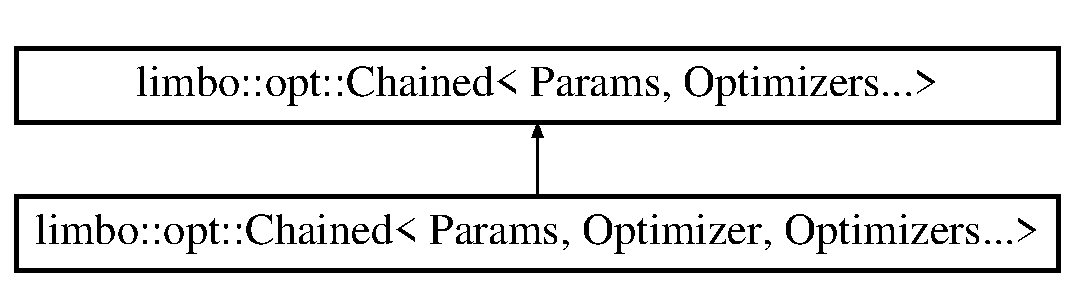
\includegraphics[height=2.000000cm]{structlimbo_1_1opt_1_1_chained_3_01_params_00_01_optimizer_00_01_optimizers_8_8_8_4}
\end{center}
\end{figure}
\subsection*{Public Member Functions}
\begin{DoxyCompactItemize}
\item 
{\footnotesize template$<$typename F $>$ }\\Eigen\+::\+Vector\+Xd \hyperlink{structlimbo_1_1opt_1_1_chained_3_01_params_00_01_optimizer_00_01_optimizers_8_8_8_4_a02bcc74dcdc42d685baaf277886fc8e5}{operator()} (const F \&f, const Eigen\+::\+Vector\+Xd \&init, bool bounded) const 
\end{DoxyCompactItemize}


\subsection{Member Function Documentation}
\hypertarget{structlimbo_1_1opt_1_1_chained_3_01_params_00_01_optimizer_00_01_optimizers_8_8_8_4_a02bcc74dcdc42d685baaf277886fc8e5}{}\index{limbo\+::opt\+::\+Chained$<$ Params, Optimizer, Optimizers...$>$@{limbo\+::opt\+::\+Chained$<$ Params, Optimizer, Optimizers...$>$}!operator()@{operator()}}
\index{operator()@{operator()}!limbo\+::opt\+::\+Chained$<$ Params, Optimizer, Optimizers...$>$@{limbo\+::opt\+::\+Chained$<$ Params, Optimizer, Optimizers...$>$}}
\subsubsection[{operator()}]{\setlength{\rightskip}{0pt plus 5cm}template$<$typename Params , typename Optimizer , typename... Optimizers$>$ template$<$typename F $>$ Eigen\+::\+Vector\+Xd {\bf limbo\+::opt\+::\+Chained}$<$ Params, Optimizer, Optimizers...$>$\+::operator() (
\begin{DoxyParamCaption}
\item[{const F \&}]{f, }
\item[{const Eigen\+::\+Vector\+Xd \&}]{init, }
\item[{bool}]{bounded}
\end{DoxyParamCaption}
) const\hspace{0.3cm}{\ttfamily [inline]}}\label{structlimbo_1_1opt_1_1_chained_3_01_params_00_01_optimizer_00_01_optimizers_8_8_8_4_a02bcc74dcdc42d685baaf277886fc8e5}


The documentation for this struct was generated from the following file\+:\begin{DoxyCompactItemize}
\item 
/tmp/doc\+\_\+limbo/limbo/src/limbo/opt/\hyperlink{chained_8hpp}{chained.\+hpp}\end{DoxyCompactItemize}

\hypertarget{structlimbo_1_1opt_1_1_cmaes}{}\section{limbo\+:\+:opt\+:\+:Cmaes$<$ Params $>$ Struct Template Reference}
\label{structlimbo_1_1opt_1_1_cmaes}\index{limbo\+::opt\+::\+Cmaes$<$ Params $>$@{limbo\+::opt\+::\+Cmaes$<$ Params $>$}}


{\ttfamily \#include $<$limbo/opt/cmaes.\+hpp$>$}

\subsection*{Public Member Functions}
\begin{DoxyCompactItemize}
\item 
{\footnotesize template$<$typename F $>$ }\\Eigen\+::\+Vector\+Xd \hyperlink{structlimbo_1_1opt_1_1_cmaes_a47ee6970bd2300108c83281ea6fced17}{operator()} (const F \&f, const Eigen\+::\+Vector\+Xd \&init, double bounded) const 
\end{DoxyCompactItemize}


\subsection{Detailed Description}
\subsubsection*{template$<$typename Params$>$struct limbo\+::opt\+::\+Cmaes$<$ Params $>$}

Covariance Matrix Adaptation Evolution Strategy by Hansen et al. (See\+: \href{https://www.lri.fr/~hansen/cmaesintro.html}{\tt https\+://www.\+lri.\+fr/$\sim$hansen/cmaesintro.\+html})
\begin{DoxyItemize}
\item our implementation is based on libcmaes (\href{https://github.com/beniz/libcmaes}{\tt https\+://github.\+com/beniz/libcmaes})
\item Support bounded and unbounded optimization
\item Only available if libcmaes is installed (see the compilation instructions)
\item Parameters \+:
\begin{DoxyItemize}
\item int variant
\item int elitism
\item int restarts
\item double max\+\_\+fun\+\_\+evals
\item double fun\+\_\+tolerance
\item double fun\+\_\+target
\item bool fun\+\_\+compute\+\_\+initial
\item bool handle\+\_\+uncertainty
\item bool verbose
\item double lb (lower bounds)
\item double ub (upper bounds) 
\end{DoxyItemize}
\end{DoxyItemize}

\subsection{Member Function Documentation}
\hypertarget{structlimbo_1_1opt_1_1_cmaes_a47ee6970bd2300108c83281ea6fced17}{}\index{limbo\+::opt\+::\+Cmaes@{limbo\+::opt\+::\+Cmaes}!operator()@{operator()}}
\index{operator()@{operator()}!limbo\+::opt\+::\+Cmaes@{limbo\+::opt\+::\+Cmaes}}
\subsubsection[{operator()}]{\setlength{\rightskip}{0pt plus 5cm}template$<$typename Params $>$ template$<$typename F $>$ Eigen\+::\+Vector\+Xd {\bf limbo\+::opt\+::\+Cmaes}$<$ Params $>$\+::operator() (
\begin{DoxyParamCaption}
\item[{const F \&}]{f, }
\item[{const Eigen\+::\+Vector\+Xd \&}]{init, }
\item[{double}]{bounded}
\end{DoxyParamCaption}
) const\hspace{0.3cm}{\ttfamily [inline]}}\label{structlimbo_1_1opt_1_1_cmaes_a47ee6970bd2300108c83281ea6fced17}


The documentation for this struct was generated from the following file\+:\begin{DoxyCompactItemize}
\item 
/tmp/doc\+\_\+limbo/limbo/src/limbo/opt/\hyperlink{cmaes_8hpp}{cmaes.\+hpp}\end{DoxyCompactItemize}

\hypertarget{structpareto_1_1impl_1_1comp__fronts}{}\section{pareto\+:\+:impl\+:\+:comp\+\_\+fronts$<$ K $>$ Struct Template Reference}
\label{structpareto_1_1impl_1_1comp__fronts}\index{pareto\+::impl\+::comp\+\_\+fronts$<$ K $>$@{pareto\+::impl\+::comp\+\_\+fronts$<$ K $>$}}


{\ttfamily \#include $<$limbo/experimental/tools/pareto.\+hpp$>$}

\subsection*{Public Member Functions}
\begin{DoxyCompactItemize}
\item 
{\footnotesize template$<$typename T $>$ }\\bool \hyperlink{structpareto_1_1impl_1_1comp__fronts_a009b840d878c3ef895ddfe34f330fdb9}{operator()} (const T \&f2, const T \&f1) const 
\end{DoxyCompactItemize}


\subsection{Member Function Documentation}
\hypertarget{structpareto_1_1impl_1_1comp__fronts_a009b840d878c3ef895ddfe34f330fdb9}{}\index{pareto\+::impl\+::comp\+\_\+fronts@{pareto\+::impl\+::comp\+\_\+fronts}!operator()@{operator()}}
\index{operator()@{operator()}!pareto\+::impl\+::comp\+\_\+fronts@{pareto\+::impl\+::comp\+\_\+fronts}}
\subsubsection[{operator()}]{\setlength{\rightskip}{0pt plus 5cm}template$<$int K$>$ template$<$typename T $>$ bool {\bf pareto\+::impl\+::comp\+\_\+fronts}$<$ K $>$\+::operator() (
\begin{DoxyParamCaption}
\item[{const T \&}]{f2, }
\item[{const T \&}]{f1}
\end{DoxyParamCaption}
) const\hspace{0.3cm}{\ttfamily [inline]}}\label{structpareto_1_1impl_1_1comp__fronts_a009b840d878c3ef895ddfe34f330fdb9}


The documentation for this struct was generated from the following file\+:\begin{DoxyCompactItemize}
\item 
/tmp/doc\+\_\+limbo/limbo/src/limbo/experimental/tools/\hyperlink{pareto_8hpp}{pareto.\+hpp}\end{DoxyCompactItemize}

\hypertarget{structpareto_1_1impl_1_1compare__objs__lex}{}\section{pareto\+:\+:impl\+:\+:compare\+\_\+objs\+\_\+lex$<$ K $>$ Struct Template Reference}
\label{structpareto_1_1impl_1_1compare__objs__lex}\index{pareto\+::impl\+::compare\+\_\+objs\+\_\+lex$<$ K $>$@{pareto\+::impl\+::compare\+\_\+objs\+\_\+lex$<$ K $>$}}


{\ttfamily \#include $<$limbo/experimental/tools/pareto.\+hpp$>$}

\subsection*{Public Member Functions}
\begin{DoxyCompactItemize}
\item 
\hyperlink{structpareto_1_1impl_1_1compare__objs__lex_a0141f68fca61380d69773bc6225622e3}{compare\+\_\+objs\+\_\+lex} ()
\item 
{\footnotesize template$<$typename T $>$ }\\bool \hyperlink{structpareto_1_1impl_1_1compare__objs__lex_a9cf3c3888c0302c3aaca3056779cc4b9}{operator()} (const T \&i1, const T \&i2) const 
\end{DoxyCompactItemize}


\subsection{Constructor \& Destructor Documentation}
\index{pareto\+::impl\+::compare\+\_\+objs\+\_\+lex@{pareto\+::impl\+::compare\+\_\+objs\+\_\+lex}!compare\+\_\+objs\+\_\+lex@{compare\+\_\+objs\+\_\+lex}}
\index{compare\+\_\+objs\+\_\+lex@{compare\+\_\+objs\+\_\+lex}!pareto\+::impl\+::compare\+\_\+objs\+\_\+lex@{pareto\+::impl\+::compare\+\_\+objs\+\_\+lex}}
\subsubsection[{\texorpdfstring{compare\+\_\+objs\+\_\+lex()}{compare_objs_lex()}}]{\setlength{\rightskip}{0pt plus 5cm}template$<$int K$>$ {\bf pareto\+::impl\+::compare\+\_\+objs\+\_\+lex}$<$ K $>$\+::{\bf compare\+\_\+objs\+\_\+lex} (
\begin{DoxyParamCaption}
{}
\end{DoxyParamCaption}
)\hspace{0.3cm}{\ttfamily [inline]}}\hypertarget{structpareto_1_1impl_1_1compare__objs__lex_a0141f68fca61380d69773bc6225622e3}{}\label{structpareto_1_1impl_1_1compare__objs__lex_a0141f68fca61380d69773bc6225622e3}


\subsection{Member Function Documentation}
\index{pareto\+::impl\+::compare\+\_\+objs\+\_\+lex@{pareto\+::impl\+::compare\+\_\+objs\+\_\+lex}!operator()@{operator()}}
\index{operator()@{operator()}!pareto\+::impl\+::compare\+\_\+objs\+\_\+lex@{pareto\+::impl\+::compare\+\_\+objs\+\_\+lex}}
\subsubsection[{\texorpdfstring{operator()(const T \&i1, const T \&i2) const }{operator()(const T &i1, const T &i2) const }}]{\setlength{\rightskip}{0pt plus 5cm}template$<$int K$>$ template$<$typename T $>$ bool {\bf pareto\+::impl\+::compare\+\_\+objs\+\_\+lex}$<$ K $>$\+::operator() (
\begin{DoxyParamCaption}
\item[{const T \&}]{i1, }
\item[{const T \&}]{i2}
\end{DoxyParamCaption}
) const\hspace{0.3cm}{\ttfamily [inline]}}\hypertarget{structpareto_1_1impl_1_1compare__objs__lex_a9cf3c3888c0302c3aaca3056779cc4b9}{}\label{structpareto_1_1impl_1_1compare__objs__lex_a9cf3c3888c0302c3aaca3056779cc4b9}


The documentation for this struct was generated from the following file\+:\begin{DoxyCompactItemize}
\item 
/tmp/doc\+\_\+limbo/limbo/src/limbo/experimental/tools/\hyperlink{pareto_8hpp}{pareto.\+hpp}\end{DoxyCompactItemize}

\hypertarget{structlimbo_1_1stat_1_1_console_summary}{}\section{limbo\+:\+:stat\+:\+:Console\+Summary$<$ Params $>$ Struct Template Reference}
\label{structlimbo_1_1stat_1_1_console_summary}\index{limbo\+::stat\+::\+Console\+Summary$<$ Params $>$@{limbo\+::stat\+::\+Console\+Summary$<$ Params $>$}}


{\ttfamily \#include $<$limbo/stat/console\+\_\+summary.\+hpp$>$}

Inheritance diagram for limbo\+:\+:stat\+:\+:Console\+Summary$<$ Params $>$\+:\begin{figure}[H]
\begin{center}
\leavevmode
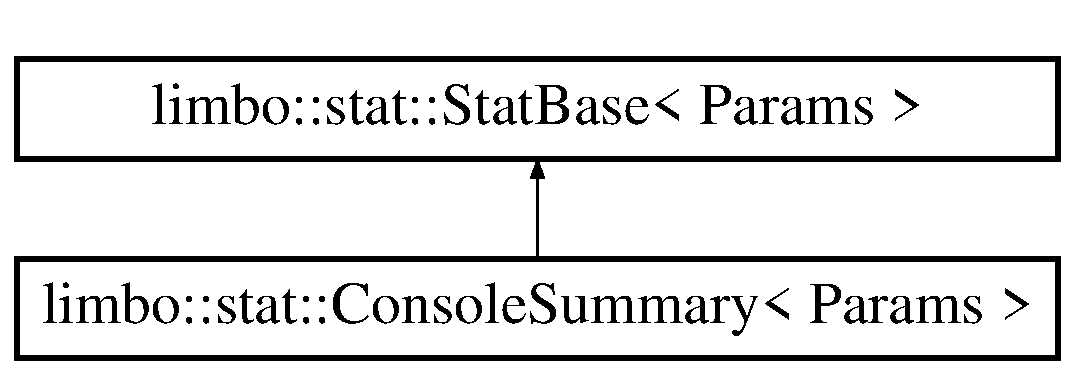
\includegraphics[height=2.000000cm]{structlimbo_1_1stat_1_1_console_summary}
\end{center}
\end{figure}
\subsection*{Public Member Functions}
\begin{DoxyCompactItemize}
\item 
{\footnotesize template$<$typename BO , typename Aggregator\+Function $>$ }\\void \hyperlink{structlimbo_1_1stat_1_1_console_summary_a7c65e2f910881abe72e4bb181d357f4a}{operator()} (const BO \&bo, const Aggregator\+Function \&afun)
\end{DoxyCompactItemize}


\subsection{Detailed Description}
\subsubsection*{template$<$typename Params$>$\\*
struct limbo\+::stat\+::\+Console\+Summary$<$ Params $>$}

write the status of the algorithm on the terminal 

\subsection{Member Function Documentation}
\index{limbo\+::stat\+::\+Console\+Summary@{limbo\+::stat\+::\+Console\+Summary}!operator()@{operator()}}
\index{operator()@{operator()}!limbo\+::stat\+::\+Console\+Summary@{limbo\+::stat\+::\+Console\+Summary}}
\subsubsection[{\texorpdfstring{operator()(const B\+O \&bo, const Aggregator\+Function \&afun)}{operator()(const BO &bo, const AggregatorFunction &afun)}}]{\setlength{\rightskip}{0pt plus 5cm}template$<$typename Params $>$ template$<$typename BO , typename Aggregator\+Function $>$ void {\bf limbo\+::stat\+::\+Console\+Summary}$<$ Params $>$\+::operator() (
\begin{DoxyParamCaption}
\item[{const BO \&}]{bo, }
\item[{const Aggregator\+Function \&}]{afun}
\end{DoxyParamCaption}
)\hspace{0.3cm}{\ttfamily [inline]}}\hypertarget{structlimbo_1_1stat_1_1_console_summary_a7c65e2f910881abe72e4bb181d357f4a}{}\label{structlimbo_1_1stat_1_1_console_summary_a7c65e2f910881abe72e4bb181d357f4a}


The documentation for this struct was generated from the following file\+:\begin{DoxyCompactItemize}
\item 
/tmp/doc\+\_\+limbo/limbo/src/limbo/stat/\hyperlink{console__summary_8hpp}{console\+\_\+summary.\+hpp}\end{DoxyCompactItemize}

\hypertarget{structlimbo_1_1mean_1_1_constant}{}\section{limbo\+:\+:mean\+:\+:Constant$<$ Params $>$ Struct Template Reference}
\label{structlimbo_1_1mean_1_1_constant}\index{limbo\+::mean\+::\+Constant$<$ Params $>$@{limbo\+::mean\+::\+Constant$<$ Params $>$}}


{\ttfamily \#include $<$limbo/mean/constant.\+hpp$>$}

\subsection*{Public Member Functions}
\begin{DoxyCompactItemize}
\item 
\hyperlink{structlimbo_1_1mean_1_1_constant_a263296f6d6b10aa360727137588735f7}{Constant} (size\+\_\+t dim\+\_\+out=1)
\item 
{\footnotesize template$<$typename G\+P $>$ }\\Eigen\+::\+Vector\+Xd \hyperlink{structlimbo_1_1mean_1_1_constant_a6ea7d6a07dfb9a45cefe9717dd25030b}{operator()} (const Eigen\+::\+Vector\+Xd \&v, const G\+P \&) const 
\end{DoxyCompactItemize}


\subsection{Detailed Description}
\subsubsection*{template$<$typename Params$>$struct limbo\+::mean\+::\+Constant$<$ Params $>$}

A constant mean (the traditionnal choice for Bayesian optimization)

Parameter\+: double constant 

\subsection{Constructor \& Destructor Documentation}
\hypertarget{structlimbo_1_1mean_1_1_constant_a263296f6d6b10aa360727137588735f7}{}\index{limbo\+::mean\+::\+Constant@{limbo\+::mean\+::\+Constant}!Constant@{Constant}}
\index{Constant@{Constant}!limbo\+::mean\+::\+Constant@{limbo\+::mean\+::\+Constant}}
\subsubsection[{Constant}]{\setlength{\rightskip}{0pt plus 5cm}template$<$typename Params $>$ {\bf limbo\+::mean\+::\+Constant}$<$ Params $>$\+::{\bf Constant} (
\begin{DoxyParamCaption}
\item[{size\+\_\+t}]{dim\+\_\+out = {\ttfamily 1}}
\end{DoxyParamCaption}
)\hspace{0.3cm}{\ttfamily [inline]}}\label{structlimbo_1_1mean_1_1_constant_a263296f6d6b10aa360727137588735f7}


\subsection{Member Function Documentation}
\hypertarget{structlimbo_1_1mean_1_1_constant_a6ea7d6a07dfb9a45cefe9717dd25030b}{}\index{limbo\+::mean\+::\+Constant@{limbo\+::mean\+::\+Constant}!operator()@{operator()}}
\index{operator()@{operator()}!limbo\+::mean\+::\+Constant@{limbo\+::mean\+::\+Constant}}
\subsubsection[{operator()}]{\setlength{\rightskip}{0pt plus 5cm}template$<$typename Params $>$ template$<$typename G\+P $>$ Eigen\+::\+Vector\+Xd {\bf limbo\+::mean\+::\+Constant}$<$ Params $>$\+::operator() (
\begin{DoxyParamCaption}
\item[{const Eigen\+::\+Vector\+Xd \&}]{v, }
\item[{const G\+P \&}]{}
\end{DoxyParamCaption}
) const\hspace{0.3cm}{\ttfamily [inline]}}\label{structlimbo_1_1mean_1_1_constant_a6ea7d6a07dfb9a45cefe9717dd25030b}


The documentation for this struct was generated from the following file\+:\begin{DoxyCompactItemize}
\item 
/tmp/doc\+\_\+limbo/limbo/src/limbo/mean/\hyperlink{constant_8hpp}{constant.\+hpp}\end{DoxyCompactItemize}

\hypertarget{structlimbo_1_1mean_1_1_data}{}\section{limbo\+:\+:mean\+:\+:Data$<$ Params $>$ Struct Template Reference}
\label{structlimbo_1_1mean_1_1_data}\index{limbo\+::mean\+::\+Data$<$ Params $>$@{limbo\+::mean\+::\+Data$<$ Params $>$}}


{\ttfamily \#include $<$limbo/mean/data.\+hpp$>$}

\subsection*{Public Member Functions}
\begin{DoxyCompactItemize}
\item 
\hyperlink{structlimbo_1_1mean_1_1_data_aedfef0dbf9ef90dd910eb11883dd2ba4}{Data} (size\+\_\+t dim\+\_\+out=1)
\item 
{\footnotesize template$<$typename GP $>$ }\\Eigen\+::\+Vector\+Xd \hyperlink{structlimbo_1_1mean_1_1_data_a68c22daf948a8367802ba6747f373a81}{operator()} (const Eigen\+::\+Vector\+Xd \&v, const GP \&gp) const 
\end{DoxyCompactItemize}


\subsection{Detailed Description}
\subsubsection*{template$<$typename Params$>$\\*
struct limbo\+::mean\+::\+Data$<$ Params $>$}

Use the mean of the observation as a constant mean 

\subsection{Constructor \& Destructor Documentation}
\index{limbo\+::mean\+::\+Data@{limbo\+::mean\+::\+Data}!Data@{Data}}
\index{Data@{Data}!limbo\+::mean\+::\+Data@{limbo\+::mean\+::\+Data}}
\subsubsection[{\texorpdfstring{Data(size\+\_\+t dim\+\_\+out=1)}{Data(size_t dim_out=1)}}]{\setlength{\rightskip}{0pt plus 5cm}template$<$typename Params $>$ {\bf limbo\+::mean\+::\+Data}$<$ Params $>$\+::{\bf Data} (
\begin{DoxyParamCaption}
\item[{size\+\_\+t}]{dim\+\_\+out = {\ttfamily 1}}
\end{DoxyParamCaption}
)\hspace{0.3cm}{\ttfamily [inline]}}\hypertarget{structlimbo_1_1mean_1_1_data_aedfef0dbf9ef90dd910eb11883dd2ba4}{}\label{structlimbo_1_1mean_1_1_data_aedfef0dbf9ef90dd910eb11883dd2ba4}


\subsection{Member Function Documentation}
\index{limbo\+::mean\+::\+Data@{limbo\+::mean\+::\+Data}!operator()@{operator()}}
\index{operator()@{operator()}!limbo\+::mean\+::\+Data@{limbo\+::mean\+::\+Data}}
\subsubsection[{\texorpdfstring{operator()(const Eigen\+::\+Vector\+Xd \&v, const G\+P \&gp) const }{operator()(const Eigen::VectorXd &v, const GP &gp) const }}]{\setlength{\rightskip}{0pt plus 5cm}template$<$typename Params $>$ template$<$typename GP $>$ Eigen\+::\+Vector\+Xd {\bf limbo\+::mean\+::\+Data}$<$ Params $>$\+::operator() (
\begin{DoxyParamCaption}
\item[{const Eigen\+::\+Vector\+Xd \&}]{v, }
\item[{const GP \&}]{gp}
\end{DoxyParamCaption}
) const\hspace{0.3cm}{\ttfamily [inline]}}\hypertarget{structlimbo_1_1mean_1_1_data_a68c22daf948a8367802ba6747f373a81}{}\label{structlimbo_1_1mean_1_1_data_a68c22daf948a8367802ba6747f373a81}


The documentation for this struct was generated from the following file\+:\begin{DoxyCompactItemize}
\item 
/tmp/doc\+\_\+limbo/limbo/src/limbo/mean/\hyperlink{data_8hpp}{data.\+hpp}\end{DoxyCompactItemize}

\hypertarget{structlimbo_1_1experimental_1_1bayes__opt_1_1_ehvi_1_1defaults}{}\section{limbo\+:\+:experimental\+:\+:bayes\+\_\+opt\+:\+:Ehvi$<$ Params, A1, A2, A3, A4, A5, A6 $>$\+:\+:defaults Struct Reference}
\label{structlimbo_1_1experimental_1_1bayes__opt_1_1_ehvi_1_1defaults}\index{limbo\+::experimental\+::bayes\+\_\+opt\+::\+Ehvi$<$ Params, A1, A2, A3, A4, A5, A6 $>$\+::defaults@{limbo\+::experimental\+::bayes\+\_\+opt\+::\+Ehvi$<$ Params, A1, A2, A3, A4, A5, A6 $>$\+::defaults}}


{\ttfamily \#include $<$limbo/experimental/bayes\+\_\+opt/ehvi.\+hpp$>$}

\subsection*{Public Types}
\begin{DoxyCompactItemize}
\item 
typedef \hyperlink{structlimbo_1_1opt_1_1_cmaes}{opt\+::\+Cmaes}$<$ Params $>$ \hyperlink{structlimbo_1_1experimental_1_1bayes__opt_1_1_ehvi_1_1defaults_a3de3f3a53d396b50e0358661f122d450}{acquiopt\+\_\+t}
\end{DoxyCompactItemize}


\subsection{Member Typedef Documentation}
\hypertarget{structlimbo_1_1experimental_1_1bayes__opt_1_1_ehvi_1_1defaults_a3de3f3a53d396b50e0358661f122d450}{}\index{limbo\+::experimental\+::bayes\+\_\+opt\+::\+Ehvi\+::defaults@{limbo\+::experimental\+::bayes\+\_\+opt\+::\+Ehvi\+::defaults}!acquiopt\+\_\+t@{acquiopt\+\_\+t}}
\index{acquiopt\+\_\+t@{acquiopt\+\_\+t}!limbo\+::experimental\+::bayes\+\_\+opt\+::\+Ehvi\+::defaults@{limbo\+::experimental\+::bayes\+\_\+opt\+::\+Ehvi\+::defaults}}
\subsubsection[{acquiopt\+\_\+t}]{\setlength{\rightskip}{0pt plus 5cm}template$<$class Params , class A1  = boost\+::parameter\+::void\+\_\+, class A2  = boost\+::parameter\+::void\+\_\+, class A3  = boost\+::parameter\+::void\+\_\+, class A4  = boost\+::parameter\+::void\+\_\+, class A5  = boost\+::parameter\+::void\+\_\+, class A6  = boost\+::parameter\+::void\+\_\+$>$ typedef {\bf opt\+::\+Cmaes}$<$Params$>$ {\bf limbo\+::experimental\+::bayes\+\_\+opt\+::\+Ehvi}$<$ Params, A1, A2, A3, A4, A5, A6 $>$\+::{\bf defaults\+::acquiopt\+\_\+t}}\label{structlimbo_1_1experimental_1_1bayes__opt_1_1_ehvi_1_1defaults_a3de3f3a53d396b50e0358661f122d450}


The documentation for this struct was generated from the following file\+:\begin{DoxyCompactItemize}
\item 
/tmp/doc\+\_\+limbo/limbo/src/limbo/experimental/bayes\+\_\+opt/\hyperlink{bayes__opt_2ehvi_8hpp}{ehvi.\+hpp}\end{DoxyCompactItemize}

\hypertarget{structlimbo_1_1bayes__opt_1_1_bo_base_1_1defaults}{}\section{limbo\+:\+:bayes\+\_\+opt\+:\+:Bo\+Base$<$ Params, A1, A2, A3, A4, A5, A6 $>$\+:\+:defaults Struct Reference}
\label{structlimbo_1_1bayes__opt_1_1_bo_base_1_1defaults}\index{limbo\+::bayes\+\_\+opt\+::\+Bo\+Base$<$ Params, A1, A2, A3, A4, A5, A6 $>$\+::defaults@{limbo\+::bayes\+\_\+opt\+::\+Bo\+Base$<$ Params, A1, A2, A3, A4, A5, A6 $>$\+::defaults}}


{\ttfamily \#include $<$limbo/bayes\+\_\+opt/bo\+\_\+base.\+hpp$>$}

\subsection*{Public Types}
\begin{DoxyCompactItemize}
\item 
using \hyperlink{structlimbo_1_1bayes__opt_1_1_bo_base_1_1defaults_afab889d523b8c28d1161079a5a453f79}{init\+\_\+t} = \hyperlink{structlimbo_1_1init_1_1_random_sampling}{init\+::\+Random\+Sampling}$<$ Params $>$
\item 
using \hyperlink{structlimbo_1_1bayes__opt_1_1_bo_base_1_1defaults_a74f559358b99209461a1aac1e0dacb1f}{kf\+\_\+t} = \hyperlink{structlimbo_1_1kernel_1_1_exp}{kernel\+::\+Exp}$<$ Params $>$
\item 
using \hyperlink{structlimbo_1_1bayes__opt_1_1_bo_base_1_1defaults_ae8b922abc8e126f785e1001342cf47ae}{mean\+\_\+t} = \hyperlink{structlimbo_1_1mean_1_1_data}{mean\+::\+Data}$<$ Params $>$
\item 
using \hyperlink{structlimbo_1_1bayes__opt_1_1_bo_base_1_1defaults_aa9a30c408b869fd46861b028b6325b4a}{model\+\_\+t} = \hyperlink{classlimbo_1_1model_1_1_g_p}{model\+::\+GP}$<$ Params, \hyperlink{structlimbo_1_1bayes__opt_1_1_bo_base_1_1defaults_a74f559358b99209461a1aac1e0dacb1f}{kf\+\_\+t}, \hyperlink{structlimbo_1_1bayes__opt_1_1_bo_base_1_1defaults_ae8b922abc8e126f785e1001342cf47ae}{mean\+\_\+t} $>$
\item 
using \hyperlink{structlimbo_1_1bayes__opt_1_1_bo_base_1_1defaults_a7728ece1763ffbcac4e37f219047dcb1}{acqui\+\_\+t} = \hyperlink{classlimbo_1_1acqui_1_1_u_c_b}{acqui\+::\+U\+CB}$<$ Params, \hyperlink{structlimbo_1_1bayes__opt_1_1_bo_base_1_1defaults_aa9a30c408b869fd46861b028b6325b4a}{model\+\_\+t} $>$
\item 
using \hyperlink{structlimbo_1_1bayes__opt_1_1_bo_base_1_1defaults_a3c475362a937e011e02c715e8edbf2d1}{stat\+\_\+t} = boost\+::fusion\+::vector$<$ \hyperlink{structlimbo_1_1stat_1_1_samples}{stat\+::\+Samples}$<$ Params $>$, \hyperlink{structlimbo_1_1stat_1_1_aggregated_observations}{stat\+::\+Aggregated\+Observations}$<$ Params $>$, \hyperlink{structlimbo_1_1stat_1_1_console_summary}{stat\+::\+Console\+Summary}$<$ Params $>$$>$
\item 
using \hyperlink{structlimbo_1_1bayes__opt_1_1_bo_base_1_1defaults_aabb9a88029b7b3cba6d1bafe3dfadaf5}{stop\+\_\+t} = boost\+::fusion\+::vector$<$ \hyperlink{structlimbo_1_1stop_1_1_max_iterations}{stop\+::\+Max\+Iterations}$<$ Params $>$$>$
\end{DoxyCompactItemize}


\subsection{Member Typedef Documentation}
\index{limbo\+::bayes\+\_\+opt\+::\+Bo\+Base\+::defaults@{limbo\+::bayes\+\_\+opt\+::\+Bo\+Base\+::defaults}!acqui\+\_\+t@{acqui\+\_\+t}}
\index{acqui\+\_\+t@{acqui\+\_\+t}!limbo\+::bayes\+\_\+opt\+::\+Bo\+Base\+::defaults@{limbo\+::bayes\+\_\+opt\+::\+Bo\+Base\+::defaults}}
\subsubsection[{\texorpdfstring{acqui\+\_\+t}{acqui_t}}]{\setlength{\rightskip}{0pt plus 5cm}template$<$class Params, class A1 = boost\+::parameter\+::void\+\_\+, class A2 = boost\+::parameter\+::void\+\_\+, class A3 = boost\+::parameter\+::void\+\_\+, class A4 = boost\+::parameter\+::void\+\_\+, class A5 = boost\+::parameter\+::void\+\_\+, class A6 = boost\+::parameter\+::void\+\_\+$>$ using {\bf limbo\+::bayes\+\_\+opt\+::\+Bo\+Base}$<$ Params, A1, A2, A3, A4, A5, A6 $>$\+::{\bf defaults\+::acqui\+\_\+t} =  {\bf acqui\+::\+U\+CB}$<$Params, {\bf model\+\_\+t}$>$}\hypertarget{structlimbo_1_1bayes__opt_1_1_bo_base_1_1defaults_a7728ece1763ffbcac4e37f219047dcb1}{}\label{structlimbo_1_1bayes__opt_1_1_bo_base_1_1defaults_a7728ece1763ffbcac4e37f219047dcb1}
\index{limbo\+::bayes\+\_\+opt\+::\+Bo\+Base\+::defaults@{limbo\+::bayes\+\_\+opt\+::\+Bo\+Base\+::defaults}!init\+\_\+t@{init\+\_\+t}}
\index{init\+\_\+t@{init\+\_\+t}!limbo\+::bayes\+\_\+opt\+::\+Bo\+Base\+::defaults@{limbo\+::bayes\+\_\+opt\+::\+Bo\+Base\+::defaults}}
\subsubsection[{\texorpdfstring{init\+\_\+t}{init_t}}]{\setlength{\rightskip}{0pt plus 5cm}template$<$class Params, class A1 = boost\+::parameter\+::void\+\_\+, class A2 = boost\+::parameter\+::void\+\_\+, class A3 = boost\+::parameter\+::void\+\_\+, class A4 = boost\+::parameter\+::void\+\_\+, class A5 = boost\+::parameter\+::void\+\_\+, class A6 = boost\+::parameter\+::void\+\_\+$>$ using {\bf limbo\+::bayes\+\_\+opt\+::\+Bo\+Base}$<$ Params, A1, A2, A3, A4, A5, A6 $>$\+::{\bf defaults\+::init\+\_\+t} =  {\bf init\+::\+Random\+Sampling}$<$Params$>$}\hypertarget{structlimbo_1_1bayes__opt_1_1_bo_base_1_1defaults_afab889d523b8c28d1161079a5a453f79}{}\label{structlimbo_1_1bayes__opt_1_1_bo_base_1_1defaults_afab889d523b8c28d1161079a5a453f79}
\index{limbo\+::bayes\+\_\+opt\+::\+Bo\+Base\+::defaults@{limbo\+::bayes\+\_\+opt\+::\+Bo\+Base\+::defaults}!kf\+\_\+t@{kf\+\_\+t}}
\index{kf\+\_\+t@{kf\+\_\+t}!limbo\+::bayes\+\_\+opt\+::\+Bo\+Base\+::defaults@{limbo\+::bayes\+\_\+opt\+::\+Bo\+Base\+::defaults}}
\subsubsection[{\texorpdfstring{kf\+\_\+t}{kf_t}}]{\setlength{\rightskip}{0pt plus 5cm}template$<$class Params, class A1 = boost\+::parameter\+::void\+\_\+, class A2 = boost\+::parameter\+::void\+\_\+, class A3 = boost\+::parameter\+::void\+\_\+, class A4 = boost\+::parameter\+::void\+\_\+, class A5 = boost\+::parameter\+::void\+\_\+, class A6 = boost\+::parameter\+::void\+\_\+$>$ using {\bf limbo\+::bayes\+\_\+opt\+::\+Bo\+Base}$<$ Params, A1, A2, A3, A4, A5, A6 $>$\+::{\bf defaults\+::kf\+\_\+t} =  {\bf kernel\+::\+Exp}$<$Params$>$}\hypertarget{structlimbo_1_1bayes__opt_1_1_bo_base_1_1defaults_a74f559358b99209461a1aac1e0dacb1f}{}\label{structlimbo_1_1bayes__opt_1_1_bo_base_1_1defaults_a74f559358b99209461a1aac1e0dacb1f}
\index{limbo\+::bayes\+\_\+opt\+::\+Bo\+Base\+::defaults@{limbo\+::bayes\+\_\+opt\+::\+Bo\+Base\+::defaults}!mean\+\_\+t@{mean\+\_\+t}}
\index{mean\+\_\+t@{mean\+\_\+t}!limbo\+::bayes\+\_\+opt\+::\+Bo\+Base\+::defaults@{limbo\+::bayes\+\_\+opt\+::\+Bo\+Base\+::defaults}}
\subsubsection[{\texorpdfstring{mean\+\_\+t}{mean_t}}]{\setlength{\rightskip}{0pt plus 5cm}template$<$class Params, class A1 = boost\+::parameter\+::void\+\_\+, class A2 = boost\+::parameter\+::void\+\_\+, class A3 = boost\+::parameter\+::void\+\_\+, class A4 = boost\+::parameter\+::void\+\_\+, class A5 = boost\+::parameter\+::void\+\_\+, class A6 = boost\+::parameter\+::void\+\_\+$>$ using {\bf limbo\+::bayes\+\_\+opt\+::\+Bo\+Base}$<$ Params, A1, A2, A3, A4, A5, A6 $>$\+::{\bf defaults\+::mean\+\_\+t} =  {\bf mean\+::\+Data}$<$Params$>$}\hypertarget{structlimbo_1_1bayes__opt_1_1_bo_base_1_1defaults_ae8b922abc8e126f785e1001342cf47ae}{}\label{structlimbo_1_1bayes__opt_1_1_bo_base_1_1defaults_ae8b922abc8e126f785e1001342cf47ae}
\index{limbo\+::bayes\+\_\+opt\+::\+Bo\+Base\+::defaults@{limbo\+::bayes\+\_\+opt\+::\+Bo\+Base\+::defaults}!model\+\_\+t@{model\+\_\+t}}
\index{model\+\_\+t@{model\+\_\+t}!limbo\+::bayes\+\_\+opt\+::\+Bo\+Base\+::defaults@{limbo\+::bayes\+\_\+opt\+::\+Bo\+Base\+::defaults}}
\subsubsection[{\texorpdfstring{model\+\_\+t}{model_t}}]{\setlength{\rightskip}{0pt plus 5cm}template$<$class Params, class A1 = boost\+::parameter\+::void\+\_\+, class A2 = boost\+::parameter\+::void\+\_\+, class A3 = boost\+::parameter\+::void\+\_\+, class A4 = boost\+::parameter\+::void\+\_\+, class A5 = boost\+::parameter\+::void\+\_\+, class A6 = boost\+::parameter\+::void\+\_\+$>$ using {\bf limbo\+::bayes\+\_\+opt\+::\+Bo\+Base}$<$ Params, A1, A2, A3, A4, A5, A6 $>$\+::{\bf defaults\+::model\+\_\+t} =  {\bf model\+::\+GP}$<$Params, {\bf kf\+\_\+t}, {\bf mean\+\_\+t}$>$}\hypertarget{structlimbo_1_1bayes__opt_1_1_bo_base_1_1defaults_aa9a30c408b869fd46861b028b6325b4a}{}\label{structlimbo_1_1bayes__opt_1_1_bo_base_1_1defaults_aa9a30c408b869fd46861b028b6325b4a}
\index{limbo\+::bayes\+\_\+opt\+::\+Bo\+Base\+::defaults@{limbo\+::bayes\+\_\+opt\+::\+Bo\+Base\+::defaults}!stat\+\_\+t@{stat\+\_\+t}}
\index{stat\+\_\+t@{stat\+\_\+t}!limbo\+::bayes\+\_\+opt\+::\+Bo\+Base\+::defaults@{limbo\+::bayes\+\_\+opt\+::\+Bo\+Base\+::defaults}}
\subsubsection[{\texorpdfstring{stat\+\_\+t}{stat_t}}]{\setlength{\rightskip}{0pt plus 5cm}template$<$class Params, class A1 = boost\+::parameter\+::void\+\_\+, class A2 = boost\+::parameter\+::void\+\_\+, class A3 = boost\+::parameter\+::void\+\_\+, class A4 = boost\+::parameter\+::void\+\_\+, class A5 = boost\+::parameter\+::void\+\_\+, class A6 = boost\+::parameter\+::void\+\_\+$>$ using {\bf limbo\+::bayes\+\_\+opt\+::\+Bo\+Base}$<$ Params, A1, A2, A3, A4, A5, A6 $>$\+::{\bf defaults\+::stat\+\_\+t} =  boost\+::fusion\+::vector$<${\bf stat\+::\+Samples}$<$Params$>$, {\bf stat\+::\+Aggregated\+Observations}$<$Params$>$, {\bf stat\+::\+Console\+Summary}$<$Params$>$$>$}\hypertarget{structlimbo_1_1bayes__opt_1_1_bo_base_1_1defaults_a3c475362a937e011e02c715e8edbf2d1}{}\label{structlimbo_1_1bayes__opt_1_1_bo_base_1_1defaults_a3c475362a937e011e02c715e8edbf2d1}
\index{limbo\+::bayes\+\_\+opt\+::\+Bo\+Base\+::defaults@{limbo\+::bayes\+\_\+opt\+::\+Bo\+Base\+::defaults}!stop\+\_\+t@{stop\+\_\+t}}
\index{stop\+\_\+t@{stop\+\_\+t}!limbo\+::bayes\+\_\+opt\+::\+Bo\+Base\+::defaults@{limbo\+::bayes\+\_\+opt\+::\+Bo\+Base\+::defaults}}
\subsubsection[{\texorpdfstring{stop\+\_\+t}{stop_t}}]{\setlength{\rightskip}{0pt plus 5cm}template$<$class Params, class A1 = boost\+::parameter\+::void\+\_\+, class A2 = boost\+::parameter\+::void\+\_\+, class A3 = boost\+::parameter\+::void\+\_\+, class A4 = boost\+::parameter\+::void\+\_\+, class A5 = boost\+::parameter\+::void\+\_\+, class A6 = boost\+::parameter\+::void\+\_\+$>$ using {\bf limbo\+::bayes\+\_\+opt\+::\+Bo\+Base}$<$ Params, A1, A2, A3, A4, A5, A6 $>$\+::{\bf defaults\+::stop\+\_\+t} =  boost\+::fusion\+::vector$<${\bf stop\+::\+Max\+Iterations}$<$Params$>$$>$}\hypertarget{structlimbo_1_1bayes__opt_1_1_bo_base_1_1defaults_aabb9a88029b7b3cba6d1bafe3dfadaf5}{}\label{structlimbo_1_1bayes__opt_1_1_bo_base_1_1defaults_aabb9a88029b7b3cba6d1bafe3dfadaf5}


The documentation for this struct was generated from the following file\+:\begin{DoxyCompactItemize}
\item 
/tmp/doc\+\_\+limbo/limbo/src/limbo/bayes\+\_\+opt/\hyperlink{bo__base_8hpp}{bo\+\_\+base.\+hpp}\end{DoxyCompactItemize}

\hypertarget{structlimbo_1_1bayes__opt_1_1_b_optimizer_1_1defaults}{}\section{limbo\+:\+:bayes\+\_\+opt\+:\+:B\+Optimizer$<$ Params, A1, A2, A3, A4, A5, A6 $>$\+:\+:defaults Struct Reference}
\label{structlimbo_1_1bayes__opt_1_1_b_optimizer_1_1defaults}\index{limbo\+::bayes\+\_\+opt\+::\+B\+Optimizer$<$ Params, A1, A2, A3, A4, A5, A6 $>$\+::defaults@{limbo\+::bayes\+\_\+opt\+::\+B\+Optimizer$<$ Params, A1, A2, A3, A4, A5, A6 $>$\+::defaults}}


{\ttfamily \#include $<$limbo/bayes\+\_\+opt/boptimizer.\+hpp$>$}

\subsection*{Public Types}
\begin{DoxyCompactItemize}
\item 
using \hyperlink{structlimbo_1_1bayes__opt_1_1_b_optimizer_1_1defaults_a354391108ed6c10e11e7c356b3a08c25}{acquiopt\+\_\+t} = \hyperlink{structlimbo_1_1opt_1_1_n_l_opt_no_grad}{opt\+::\+N\+L\+Opt\+No\+Grad}$<$ Params, nlopt\+::\+G\+N\+\_\+\+D\+I\+R\+E\+C\+T\+\_\+\+L\+\_\+\+R\+A\+ND $>$
\end{DoxyCompactItemize}


\subsection{Member Typedef Documentation}
\index{limbo\+::bayes\+\_\+opt\+::\+B\+Optimizer\+::defaults@{limbo\+::bayes\+\_\+opt\+::\+B\+Optimizer\+::defaults}!acquiopt\+\_\+t@{acquiopt\+\_\+t}}
\index{acquiopt\+\_\+t@{acquiopt\+\_\+t}!limbo\+::bayes\+\_\+opt\+::\+B\+Optimizer\+::defaults@{limbo\+::bayes\+\_\+opt\+::\+B\+Optimizer\+::defaults}}
\subsubsection[{\texorpdfstring{acquiopt\+\_\+t}{acquiopt_t}}]{\setlength{\rightskip}{0pt plus 5cm}template$<$class Params, class A1 = boost\+::parameter\+::void\+\_\+, class A2 = boost\+::parameter\+::void\+\_\+, class A3 = boost\+::parameter\+::void\+\_\+, class A4 = boost\+::parameter\+::void\+\_\+, class A5 = boost\+::parameter\+::void\+\_\+, class A6 = boost\+::parameter\+::void\+\_\+$>$ using {\bf limbo\+::bayes\+\_\+opt\+::\+B\+Optimizer}$<$ Params, A1, A2, A3, A4, A5, A6 $>$\+::{\bf defaults\+::acquiopt\+\_\+t} =  {\bf opt\+::\+N\+L\+Opt\+No\+Grad}$<$Params, nlopt\+::\+G\+N\+\_\+\+D\+I\+R\+E\+C\+T\+\_\+\+L\+\_\+\+R\+A\+ND$>$}\hypertarget{structlimbo_1_1bayes__opt_1_1_b_optimizer_1_1defaults_a354391108ed6c10e11e7c356b3a08c25}{}\label{structlimbo_1_1bayes__opt_1_1_b_optimizer_1_1defaults_a354391108ed6c10e11e7c356b3a08c25}


The documentation for this struct was generated from the following file\+:\begin{DoxyCompactItemize}
\item 
/tmp/doc\+\_\+limbo/limbo/src/limbo/bayes\+\_\+opt/\hyperlink{boptimizer_8hpp}{boptimizer.\+hpp}\end{DoxyCompactItemize}

\hypertarget{classlimbo_1_1experimental_1_1bayes__opt_1_1_ehvi}{}\section{limbo\+:\+:experimental\+:\+:bayes\+\_\+opt\+:\+:Ehvi$<$ Params, A2, A3, A4, A5, A6 $>$ Class Template Reference}
\label{classlimbo_1_1experimental_1_1bayes__opt_1_1_ehvi}\index{limbo\+::experimental\+::bayes\+\_\+opt\+::\+Ehvi$<$ Params, A2, A3, A4, A5, A6 $>$@{limbo\+::experimental\+::bayes\+\_\+opt\+::\+Ehvi$<$ Params, A2, A3, A4, A5, A6 $>$}}


{\ttfamily \#include $<$limbo/experimental/bayes\+\_\+opt/ehvi.\+hpp$>$}

Inheritance diagram for limbo\+:\+:experimental\+:\+:bayes\+\_\+opt\+:\+:Ehvi$<$ Params, A2, A3, A4, A5, A6 $>$\+:\begin{figure}[H]
\begin{center}
\leavevmode
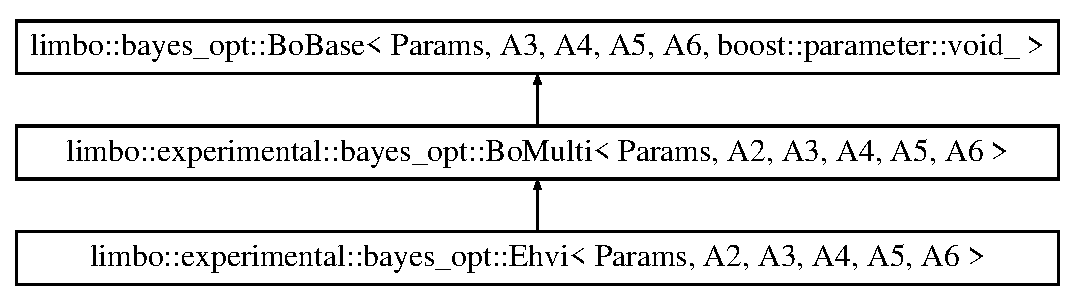
\includegraphics[height=3.000000cm]{classlimbo_1_1experimental_1_1bayes__opt_1_1_ehvi}
\end{center}
\end{figure}
\subsection*{Public Types}
\begin{DoxyCompactItemize}
\item 
typedef std\+::tuple$<$ Eigen\+::\+Vector\+Xd, Eigen\+::\+Vector\+Xd, Eigen\+::\+Vector\+Xd $>$ \hyperlink{classlimbo_1_1experimental_1_1bayes__opt_1_1_ehvi_a98176e0f540cebc76616142da6fbca6e}{pareto\+\_\+point\+\_\+t}
\item 
typedef \hyperlink{classlimbo_1_1bayes__opt_1_1_bo_base}{limbo\+::bayes\+\_\+opt\+::\+Bo\+Base}$<$ Params, A3, A4, A5, A6 $>$ \hyperlink{classlimbo_1_1experimental_1_1bayes__opt_1_1_ehvi_aab1a707afba4fe47658755ca5b66a77e}{base\+\_\+t}
\item 
typedef \hyperlink{classlimbo_1_1bayes__opt_1_1_bo_base_a1ddc93cc023a2d7d527deb4cc750624e}{base\+\_\+t\+::model\+\_\+t} \hyperlink{classlimbo_1_1experimental_1_1bayes__opt_1_1_ehvi_af9a1e49996eb15f36e08a7398e3b024e}{model\+\_\+t}
\item 
typedef base\+\_\+t\+::acqui\+\_\+optimizer\+\_\+t \hyperlink{classlimbo_1_1experimental_1_1bayes__opt_1_1_ehvi_a0bcaf7560c3d5cb4f18f2b6b3cbd521f}{acqui\+\_\+optimizer\+\_\+t}
\end{DoxyCompactItemize}
\subsection*{Public Member Functions}
\begin{DoxyCompactItemize}
\item 
{\footnotesize template$<$typename Eval\+Function $>$ }\\void \hyperlink{classlimbo_1_1experimental_1_1bayes__opt_1_1_ehvi_a8b0bf0093f587c4e0b71612049bcec6e}{optimize} (const Eval\+Function \&feval, bool reset=true)
\end{DoxyCompactItemize}


\subsection{Member Typedef Documentation}
\hypertarget{classlimbo_1_1experimental_1_1bayes__opt_1_1_ehvi_a0bcaf7560c3d5cb4f18f2b6b3cbd521f}{}\index{limbo\+::experimental\+::bayes\+\_\+opt\+::\+Ehvi@{limbo\+::experimental\+::bayes\+\_\+opt\+::\+Ehvi}!acqui\+\_\+optimizer\+\_\+t@{acqui\+\_\+optimizer\+\_\+t}}
\index{acqui\+\_\+optimizer\+\_\+t@{acqui\+\_\+optimizer\+\_\+t}!limbo\+::experimental\+::bayes\+\_\+opt\+::\+Ehvi@{limbo\+::experimental\+::bayes\+\_\+opt\+::\+Ehvi}}
\subsubsection[{acqui\+\_\+optimizer\+\_\+t}]{\setlength{\rightskip}{0pt plus 5cm}template$<$class Params , class A2  = boost\+::parameter\+::void\+\_\+, class A3  = boost\+::parameter\+::void\+\_\+, class A4  = boost\+::parameter\+::void\+\_\+, class A5  = boost\+::parameter\+::void\+\_\+, class A6  = boost\+::parameter\+::void\+\_\+$>$ typedef base\+\_\+t\+::acqui\+\_\+optimizer\+\_\+t {\bf limbo\+::experimental\+::bayes\+\_\+opt\+::\+Ehvi}$<$ Params, A2, A3, A4, A5, A6 $>$\+::{\bf acqui\+\_\+optimizer\+\_\+t}}\label{classlimbo_1_1experimental_1_1bayes__opt_1_1_ehvi_a0bcaf7560c3d5cb4f18f2b6b3cbd521f}
\hypertarget{classlimbo_1_1experimental_1_1bayes__opt_1_1_ehvi_aab1a707afba4fe47658755ca5b66a77e}{}\index{limbo\+::experimental\+::bayes\+\_\+opt\+::\+Ehvi@{limbo\+::experimental\+::bayes\+\_\+opt\+::\+Ehvi}!base\+\_\+t@{base\+\_\+t}}
\index{base\+\_\+t@{base\+\_\+t}!limbo\+::experimental\+::bayes\+\_\+opt\+::\+Ehvi@{limbo\+::experimental\+::bayes\+\_\+opt\+::\+Ehvi}}
\subsubsection[{base\+\_\+t}]{\setlength{\rightskip}{0pt plus 5cm}template$<$class Params , class A2  = boost\+::parameter\+::void\+\_\+, class A3  = boost\+::parameter\+::void\+\_\+, class A4  = boost\+::parameter\+::void\+\_\+, class A5  = boost\+::parameter\+::void\+\_\+, class A6  = boost\+::parameter\+::void\+\_\+$>$ typedef {\bf limbo\+::bayes\+\_\+opt\+::\+Bo\+Base}$<$Params, A3, A4, A5, A6$>$ {\bf limbo\+::experimental\+::bayes\+\_\+opt\+::\+Ehvi}$<$ Params, A2, A3, A4, A5, A6 $>$\+::{\bf base\+\_\+t}}\label{classlimbo_1_1experimental_1_1bayes__opt_1_1_ehvi_aab1a707afba4fe47658755ca5b66a77e}
\hypertarget{classlimbo_1_1experimental_1_1bayes__opt_1_1_ehvi_af9a1e49996eb15f36e08a7398e3b024e}{}\index{limbo\+::experimental\+::bayes\+\_\+opt\+::\+Ehvi@{limbo\+::experimental\+::bayes\+\_\+opt\+::\+Ehvi}!model\+\_\+t@{model\+\_\+t}}
\index{model\+\_\+t@{model\+\_\+t}!limbo\+::experimental\+::bayes\+\_\+opt\+::\+Ehvi@{limbo\+::experimental\+::bayes\+\_\+opt\+::\+Ehvi}}
\subsubsection[{model\+\_\+t}]{\setlength{\rightskip}{0pt plus 5cm}template$<$class Params , class A2  = boost\+::parameter\+::void\+\_\+, class A3  = boost\+::parameter\+::void\+\_\+, class A4  = boost\+::parameter\+::void\+\_\+, class A5  = boost\+::parameter\+::void\+\_\+, class A6  = boost\+::parameter\+::void\+\_\+$>$ typedef {\bf base\+\_\+t\+::model\+\_\+t} {\bf limbo\+::experimental\+::bayes\+\_\+opt\+::\+Ehvi}$<$ Params, A2, A3, A4, A5, A6 $>$\+::{\bf model\+\_\+t}}\label{classlimbo_1_1experimental_1_1bayes__opt_1_1_ehvi_af9a1e49996eb15f36e08a7398e3b024e}
\hypertarget{classlimbo_1_1experimental_1_1bayes__opt_1_1_ehvi_a98176e0f540cebc76616142da6fbca6e}{}\index{limbo\+::experimental\+::bayes\+\_\+opt\+::\+Ehvi@{limbo\+::experimental\+::bayes\+\_\+opt\+::\+Ehvi}!pareto\+\_\+point\+\_\+t@{pareto\+\_\+point\+\_\+t}}
\index{pareto\+\_\+point\+\_\+t@{pareto\+\_\+point\+\_\+t}!limbo\+::experimental\+::bayes\+\_\+opt\+::\+Ehvi@{limbo\+::experimental\+::bayes\+\_\+opt\+::\+Ehvi}}
\subsubsection[{pareto\+\_\+point\+\_\+t}]{\setlength{\rightskip}{0pt plus 5cm}template$<$class Params , class A2  = boost\+::parameter\+::void\+\_\+, class A3  = boost\+::parameter\+::void\+\_\+, class A4  = boost\+::parameter\+::void\+\_\+, class A5  = boost\+::parameter\+::void\+\_\+, class A6  = boost\+::parameter\+::void\+\_\+$>$ typedef std\+::tuple$<$Eigen\+::\+Vector\+Xd, Eigen\+::\+Vector\+Xd, Eigen\+::\+Vector\+Xd$>$ {\bf limbo\+::experimental\+::bayes\+\_\+opt\+::\+Ehvi}$<$ Params, A2, A3, A4, A5, A6 $>$\+::{\bf pareto\+\_\+point\+\_\+t}}\label{classlimbo_1_1experimental_1_1bayes__opt_1_1_ehvi_a98176e0f540cebc76616142da6fbca6e}


\subsection{Member Function Documentation}
\hypertarget{classlimbo_1_1experimental_1_1bayes__opt_1_1_ehvi_a8b0bf0093f587c4e0b71612049bcec6e}{}\index{limbo\+::experimental\+::bayes\+\_\+opt\+::\+Ehvi@{limbo\+::experimental\+::bayes\+\_\+opt\+::\+Ehvi}!optimize@{optimize}}
\index{optimize@{optimize}!limbo\+::experimental\+::bayes\+\_\+opt\+::\+Ehvi@{limbo\+::experimental\+::bayes\+\_\+opt\+::\+Ehvi}}
\subsubsection[{optimize}]{\setlength{\rightskip}{0pt plus 5cm}template$<$class Params , class A2  = boost\+::parameter\+::void\+\_\+, class A3  = boost\+::parameter\+::void\+\_\+, class A4  = boost\+::parameter\+::void\+\_\+, class A5  = boost\+::parameter\+::void\+\_\+, class A6  = boost\+::parameter\+::void\+\_\+$>$ template$<$typename Eval\+Function $>$ void {\bf limbo\+::experimental\+::bayes\+\_\+opt\+::\+Ehvi}$<$ Params, A2, A3, A4, A5, A6 $>$\+::optimize (
\begin{DoxyParamCaption}
\item[{const Eval\+Function \&}]{feval, }
\item[{bool}]{reset = {\ttfamily true}}
\end{DoxyParamCaption}
)\hspace{0.3cm}{\ttfamily [inline]}}\label{classlimbo_1_1experimental_1_1bayes__opt_1_1_ehvi_a8b0bf0093f587c4e0b71612049bcec6e}


The documentation for this class was generated from the following file\+:\begin{DoxyCompactItemize}
\item 
/tmp/doc\+\_\+limbo/limbo/src/limbo/experimental/bayes\+\_\+opt/\hyperlink{bayes__opt_2ehvi_8hpp}{ehvi.\+hpp}\end{DoxyCompactItemize}

\hypertarget{classlimbo_1_1acqui_1_1_ehvi}{}\section{limbo\+:\+:acqui\+:\+:Ehvi$<$ Params, Model $>$ Class Template Reference}
\label{classlimbo_1_1acqui_1_1_ehvi}\index{limbo\+::acqui\+::\+Ehvi$<$ Params, Model $>$@{limbo\+::acqui\+::\+Ehvi$<$ Params, Model $>$}}


{\ttfamily \#include $<$limbo/experimental/acqui/ehvi.\+hpp$>$}

\subsection*{Public Member Functions}
\begin{DoxyCompactItemize}
\item 
\hyperlink{classlimbo_1_1acqui_1_1_ehvi_a9868f015ef640e9406022b027a0d7683}{Ehvi} (const std\+::vector$<$ Model $>$ \&models, const std\+::deque$<$ individual $\ast$ $>$ \&pop, const Eigen\+::\+Vector\+Xd \&ref\+\_\+point)
\item 
size\+\_\+t \hyperlink{classlimbo_1_1acqui_1_1_ehvi_a5d0876e753a2f1037bdf264501fdbd5d}{dim} () const 
\item 
{\footnotesize template$<$typename Aggregator\+Function  = First\+Elem$>$ }\\double \hyperlink{classlimbo_1_1acqui_1_1_ehvi_a1e99fe83a965b5f706d057895598907d}{operator()} (const Eigen\+::\+Vector\+Xd \&v, const Aggregator\+Function \&afun=Aggregator\+Function()) const 
\end{DoxyCompactItemize}


\subsection{Constructor \& Destructor Documentation}
\hypertarget{classlimbo_1_1acqui_1_1_ehvi_a9868f015ef640e9406022b027a0d7683}{}\index{limbo\+::acqui\+::\+Ehvi@{limbo\+::acqui\+::\+Ehvi}!Ehvi@{Ehvi}}
\index{Ehvi@{Ehvi}!limbo\+::acqui\+::\+Ehvi@{limbo\+::acqui\+::\+Ehvi}}
\subsubsection[{Ehvi}]{\setlength{\rightskip}{0pt plus 5cm}template$<$typename Params, typename Model$>$ {\bf limbo\+::acqui\+::\+Ehvi}$<$ Params, Model $>$\+::{\bf Ehvi} (
\begin{DoxyParamCaption}
\item[{const std\+::vector$<$ Model $>$ \&}]{models, }
\item[{const std\+::deque$<$ individual $\ast$ $>$ \&}]{pop, }
\item[{const Eigen\+::\+Vector\+Xd \&}]{ref\+\_\+point}
\end{DoxyParamCaption}
)\hspace{0.3cm}{\ttfamily [inline]}}\label{classlimbo_1_1acqui_1_1_ehvi_a9868f015ef640e9406022b027a0d7683}


\subsection{Member Function Documentation}
\hypertarget{classlimbo_1_1acqui_1_1_ehvi_a5d0876e753a2f1037bdf264501fdbd5d}{}\index{limbo\+::acqui\+::\+Ehvi@{limbo\+::acqui\+::\+Ehvi}!dim@{dim}}
\index{dim@{dim}!limbo\+::acqui\+::\+Ehvi@{limbo\+::acqui\+::\+Ehvi}}
\subsubsection[{dim}]{\setlength{\rightskip}{0pt plus 5cm}template$<$typename Params, typename Model$>$ size\+\_\+t {\bf limbo\+::acqui\+::\+Ehvi}$<$ Params, Model $>$\+::dim (
\begin{DoxyParamCaption}
{}
\end{DoxyParamCaption}
) const\hspace{0.3cm}{\ttfamily [inline]}}\label{classlimbo_1_1acqui_1_1_ehvi_a5d0876e753a2f1037bdf264501fdbd5d}
\hypertarget{classlimbo_1_1acqui_1_1_ehvi_a1e99fe83a965b5f706d057895598907d}{}\index{limbo\+::acqui\+::\+Ehvi@{limbo\+::acqui\+::\+Ehvi}!operator()@{operator()}}
\index{operator()@{operator()}!limbo\+::acqui\+::\+Ehvi@{limbo\+::acqui\+::\+Ehvi}}
\subsubsection[{operator()}]{\setlength{\rightskip}{0pt plus 5cm}template$<$typename Params, typename Model$>$ template$<$typename Aggregator\+Function  = First\+Elem$>$ double {\bf limbo\+::acqui\+::\+Ehvi}$<$ Params, Model $>$\+::operator() (
\begin{DoxyParamCaption}
\item[{const Eigen\+::\+Vector\+Xd \&}]{v, }
\item[{const Aggregator\+Function \&}]{afun = {\ttfamily AggregatorFunction()}}
\end{DoxyParamCaption}
) const\hspace{0.3cm}{\ttfamily [inline]}}\label{classlimbo_1_1acqui_1_1_ehvi_a1e99fe83a965b5f706d057895598907d}


The documentation for this class was generated from the following file\+:\begin{DoxyCompactItemize}
\item 
/tmp/doc\+\_\+limbo/limbo/src/limbo/experimental/acqui/\hyperlink{acqui_2ehvi_8hpp}{ehvi.\+hpp}\end{DoxyCompactItemize}

\hypertarget{classlimbo_1_1_evaluation_error}{}\section{limbo\+:\+:Evaluation\+Error Class Reference}
\label{classlimbo_1_1_evaluation_error}\index{limbo\+::\+Evaluation\+Error@{limbo\+::\+Evaluation\+Error}}


{\ttfamily \#include $<$limbo/bayes\+\_\+opt/bo\+\_\+base.\+hpp$>$}

Inheritance diagram for limbo\+:\+:Evaluation\+Error\+:\begin{figure}[H]
\begin{center}
\leavevmode
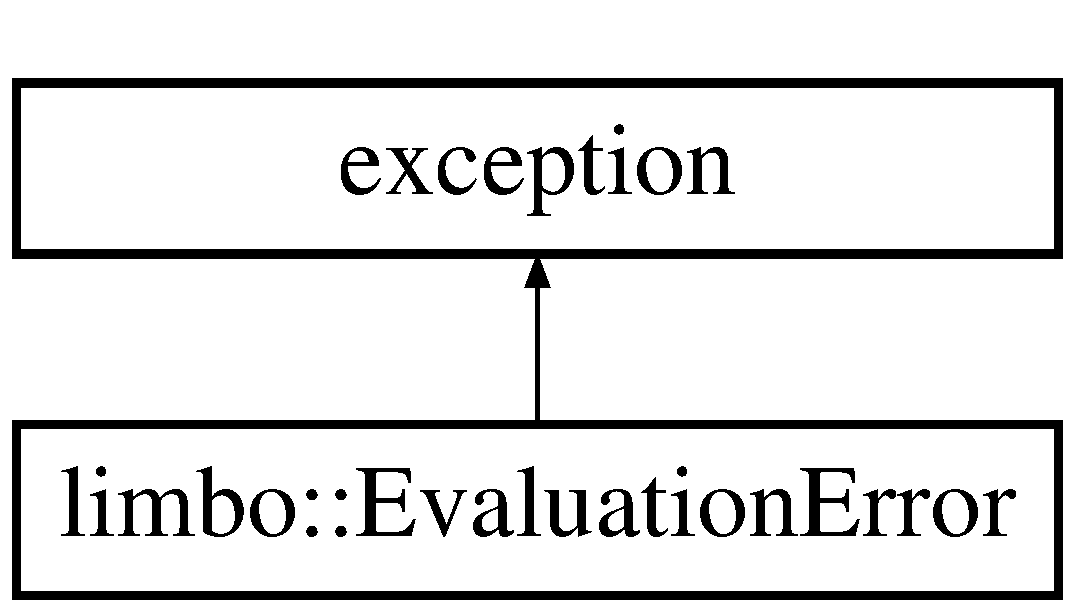
\includegraphics[height=2.000000cm]{classlimbo_1_1_evaluation_error}
\end{center}
\end{figure}


The documentation for this class was generated from the following file\+:\begin{DoxyCompactItemize}
\item 
/tmp/doc\+\_\+limbo/limbo/src/limbo/bayes\+\_\+opt/\hyperlink{bo__base_8hpp}{bo\+\_\+base.\+hpp}\end{DoxyCompactItemize}

\hypertarget{structlimbo_1_1kernel_1_1_exp}{}\section{limbo\+:\+:kernel\+:\+:Exp$<$ Params $>$ Struct Template Reference}
\label{structlimbo_1_1kernel_1_1_exp}\index{limbo\+::kernel\+::\+Exp$<$ Params $>$@{limbo\+::kernel\+::\+Exp$<$ Params $>$}}


{\ttfamily \#include $<$limbo/kernel/exp.\+hpp$>$}

Inheritance diagram for limbo\+:\+:kernel\+:\+:Exp$<$ Params $>$\+:\begin{figure}[H]
\begin{center}
\leavevmode
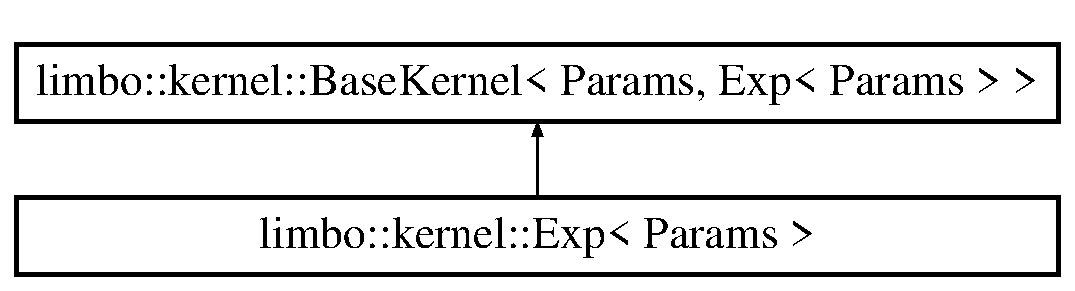
\includegraphics[height=2.000000cm]{structlimbo_1_1kernel_1_1_exp}
\end{center}
\end{figure}
\subsection*{Public Member Functions}
\begin{DoxyCompactItemize}
\item 
\hyperlink{structlimbo_1_1kernel_1_1_exp_abec48720f518fa51be7f74bf102add09}{Exp} (size\+\_\+t dim=1)
\item 
double \hyperlink{structlimbo_1_1kernel_1_1_exp_abb1accd4f07243ef60fbd9441ebeb323}{kernel} (const Eigen\+::\+Vector\+Xd \&v1, const Eigen\+::\+Vector\+Xd \&v2) const 
\end{DoxyCompactItemize}


\subsection{Detailed Description}
\subsubsection*{template$<$typename Params$>$\\*
struct limbo\+::kernel\+::\+Exp$<$ Params $>$}

\begin{DoxyVerb}embed:rst
Exponential kernel (see :cite:`brochu2010tutorial` p. 9).

.. math::
    k(v_1, v_2)  = \sigma^2\exp \Big(-\frac{1}{l^2} ||v_1 - v_2||^2\Big)

Parameters:
  - ``double sigma_sq`` (signal variance)
  - ``double l`` (characteristic length scale)
\end{DoxyVerb}
 

\subsection{Constructor \& Destructor Documentation}
\index{limbo\+::kernel\+::\+Exp@{limbo\+::kernel\+::\+Exp}!Exp@{Exp}}
\index{Exp@{Exp}!limbo\+::kernel\+::\+Exp@{limbo\+::kernel\+::\+Exp}}
\subsubsection[{\texorpdfstring{Exp(size\+\_\+t dim=1)}{Exp(size_t dim=1)}}]{\setlength{\rightskip}{0pt plus 5cm}template$<$typename Params $>$ {\bf limbo\+::kernel\+::\+Exp}$<$ Params $>$\+::{\bf Exp} (
\begin{DoxyParamCaption}
\item[{size\+\_\+t}]{dim = {\ttfamily 1}}
\end{DoxyParamCaption}
)\hspace{0.3cm}{\ttfamily [inline]}}\hypertarget{structlimbo_1_1kernel_1_1_exp_abec48720f518fa51be7f74bf102add09}{}\label{structlimbo_1_1kernel_1_1_exp_abec48720f518fa51be7f74bf102add09}


\subsection{Member Function Documentation}
\index{limbo\+::kernel\+::\+Exp@{limbo\+::kernel\+::\+Exp}!kernel@{kernel}}
\index{kernel@{kernel}!limbo\+::kernel\+::\+Exp@{limbo\+::kernel\+::\+Exp}}
\subsubsection[{\texorpdfstring{kernel(const Eigen\+::\+Vector\+Xd \&v1, const Eigen\+::\+Vector\+Xd \&v2) const }{kernel(const Eigen::VectorXd &v1, const Eigen::VectorXd &v2) const }}]{\setlength{\rightskip}{0pt plus 5cm}template$<$typename Params $>$ double {\bf limbo\+::kernel\+::\+Exp}$<$ Params $>$\+::kernel (
\begin{DoxyParamCaption}
\item[{const Eigen\+::\+Vector\+Xd \&}]{v1, }
\item[{const Eigen\+::\+Vector\+Xd \&}]{v2}
\end{DoxyParamCaption}
) const\hspace{0.3cm}{\ttfamily [inline]}}\hypertarget{structlimbo_1_1kernel_1_1_exp_abb1accd4f07243ef60fbd9441ebeb323}{}\label{structlimbo_1_1kernel_1_1_exp_abb1accd4f07243ef60fbd9441ebeb323}


The documentation for this struct was generated from the following file\+:\begin{DoxyCompactItemize}
\item 
/tmp/doc\+\_\+limbo/limbo/src/limbo/kernel/\hyperlink{exp_8hpp}{exp.\+hpp}\end{DoxyCompactItemize}

\hypertarget{structlimbo_1_1_first_elem}{}\section{limbo\+:\+:First\+Elem Struct Reference}
\label{structlimbo_1_1_first_elem}\index{limbo\+::\+First\+Elem@{limbo\+::\+First\+Elem}}


{\ttfamily \#include $<$limbo/bayes\+\_\+opt/bo\+\_\+base.\+hpp$>$}

\subsection*{Public Types}
\begin{DoxyCompactItemize}
\item 
using \hyperlink{structlimbo_1_1_first_elem_a615df66bdce08d6cb405fbe4710e3953}{result\+\_\+type} = double
\end{DoxyCompactItemize}
\subsection*{Public Member Functions}
\begin{DoxyCompactItemize}
\item 
double \hyperlink{structlimbo_1_1_first_elem_a6816ea8e21acec76f91542776ab02422}{operator()} (const Eigen\+::\+Vector\+Xd \&x) const 
\end{DoxyCompactItemize}


\subsection{Member Typedef Documentation}
\hypertarget{structlimbo_1_1_first_elem_a615df66bdce08d6cb405fbe4710e3953}{}\index{limbo\+::\+First\+Elem@{limbo\+::\+First\+Elem}!result\+\_\+type@{result\+\_\+type}}
\index{result\+\_\+type@{result\+\_\+type}!limbo\+::\+First\+Elem@{limbo\+::\+First\+Elem}}
\subsubsection[{result\+\_\+type}]{\setlength{\rightskip}{0pt plus 5cm}using {\bf limbo\+::\+First\+Elem\+::result\+\_\+type} =  double}\label{structlimbo_1_1_first_elem_a615df66bdce08d6cb405fbe4710e3953}


\subsection{Member Function Documentation}
\hypertarget{structlimbo_1_1_first_elem_a6816ea8e21acec76f91542776ab02422}{}\index{limbo\+::\+First\+Elem@{limbo\+::\+First\+Elem}!operator()@{operator()}}
\index{operator()@{operator()}!limbo\+::\+First\+Elem@{limbo\+::\+First\+Elem}}
\subsubsection[{operator()}]{\setlength{\rightskip}{0pt plus 5cm}double limbo\+::\+First\+Elem\+::operator() (
\begin{DoxyParamCaption}
\item[{const Eigen\+::\+Vector\+Xd \&}]{x}
\end{DoxyParamCaption}
) const\hspace{0.3cm}{\ttfamily [inline]}}\label{structlimbo_1_1_first_elem_a6816ea8e21acec76f91542776ab02422}


The documentation for this struct was generated from the following file\+:\begin{DoxyCompactItemize}
\item 
/tmp/doc\+\_\+limbo/limbo/src/limbo/bayes\+\_\+opt/\hyperlink{bo__base_8hpp}{bo\+\_\+base.\+hpp}\end{DoxyCompactItemize}

\hypertarget{structlimbo_1_1mean_1_1_function_a_r_d}{}\section{limbo\+:\+:mean\+:\+:Function\+A\+R\+D$<$ Params, Mean\+Function $>$ Struct Template Reference}
\label{structlimbo_1_1mean_1_1_function_a_r_d}\index{limbo\+::mean\+::\+Function\+A\+R\+D$<$ Params, Mean\+Function $>$@{limbo\+::mean\+::\+Function\+A\+R\+D$<$ Params, Mean\+Function $>$}}


{\ttfamily \#include $<$limbo/mean/function\+\_\+ard.\+hpp$>$}

\subsection*{Public Member Functions}
\begin{DoxyCompactItemize}
\item 
\hyperlink{structlimbo_1_1mean_1_1_function_a_r_d_ae43aef0e74455e5c97dd2d8cda17a0a1}{Function\+A\+R\+D} (size\+\_\+t dim\+\_\+out=1)
\item 
size\+\_\+t \hyperlink{structlimbo_1_1mean_1_1_function_a_r_d_aaf1b474fc0a0c7b9738da60bca99b45b}{h\+\_\+params\+\_\+size} () const 
\item 
const Eigen\+::\+Vector\+Xd \& \hyperlink{structlimbo_1_1mean_1_1_function_a_r_d_a4b8676c860264932e5ebd302e46e1a42}{h\+\_\+params} () const 
\item 
void \hyperlink{structlimbo_1_1mean_1_1_function_a_r_d_a02dabc2cbdf001450cdd893f578c042d}{set\+\_\+h\+\_\+params} (const Eigen\+::\+Vector\+Xd \&p)
\item 
{\footnotesize template$<$typename G\+P $>$ }\\Eigen\+::\+Matrix\+Xd \hyperlink{structlimbo_1_1mean_1_1_function_a_r_d_a5bd1343c7f3616c066296813361d9a96}{grad} (const Eigen\+::\+Vector\+Xd \&x, const G\+P \&gp) const 
\item 
{\footnotesize template$<$typename G\+P $>$ }\\Eigen\+::\+Vector\+Xd \hyperlink{structlimbo_1_1mean_1_1_function_a_r_d_acfc9ce5670a247a35a1f09e5f0a09adb}{operator()} (const Eigen\+::\+Vector\+Xd \&x, const G\+P \&gp) const 
\end{DoxyCompactItemize}


\subsection{Detailed Description}
\subsubsection*{template$<$typename Params, typename Mean\+Function$>$struct limbo\+::mean\+::\+Function\+A\+R\+D$<$ Params, Mean\+Function $>$}

Functor used to optimize the mean function using the maximum likelihood principle

\begin{DoxySeeAlso}{See also}
\hyperlink{structlimbo_1_1model_1_1gp_1_1_kernel_mean_l_f_opt}{limbo\+::model\+::gp\+::\+Kernel\+Mean\+L\+F\+Opt}, \hyperlink{structlimbo_1_1model_1_1gp_1_1_mean_l_f_opt}{limbo\+::model\+::gp\+::\+Mean\+L\+F\+Opt} 
\end{DoxySeeAlso}


\subsection{Constructor \& Destructor Documentation}
\hypertarget{structlimbo_1_1mean_1_1_function_a_r_d_ae43aef0e74455e5c97dd2d8cda17a0a1}{}\index{limbo\+::mean\+::\+Function\+A\+R\+D@{limbo\+::mean\+::\+Function\+A\+R\+D}!Function\+A\+R\+D@{Function\+A\+R\+D}}
\index{Function\+A\+R\+D@{Function\+A\+R\+D}!limbo\+::mean\+::\+Function\+A\+R\+D@{limbo\+::mean\+::\+Function\+A\+R\+D}}
\subsubsection[{Function\+A\+R\+D}]{\setlength{\rightskip}{0pt plus 5cm}template$<$typename Params , typename Mean\+Function $>$ {\bf limbo\+::mean\+::\+Function\+A\+R\+D}$<$ Params, Mean\+Function $>$\+::{\bf Function\+A\+R\+D} (
\begin{DoxyParamCaption}
\item[{size\+\_\+t}]{dim\+\_\+out = {\ttfamily 1}}
\end{DoxyParamCaption}
)\hspace{0.3cm}{\ttfamily [inline]}}\label{structlimbo_1_1mean_1_1_function_a_r_d_ae43aef0e74455e5c97dd2d8cda17a0a1}


\subsection{Member Function Documentation}
\hypertarget{structlimbo_1_1mean_1_1_function_a_r_d_a5bd1343c7f3616c066296813361d9a96}{}\index{limbo\+::mean\+::\+Function\+A\+R\+D@{limbo\+::mean\+::\+Function\+A\+R\+D}!grad@{grad}}
\index{grad@{grad}!limbo\+::mean\+::\+Function\+A\+R\+D@{limbo\+::mean\+::\+Function\+A\+R\+D}}
\subsubsection[{grad}]{\setlength{\rightskip}{0pt plus 5cm}template$<$typename Params , typename Mean\+Function $>$ template$<$typename G\+P $>$ Eigen\+::\+Matrix\+Xd {\bf limbo\+::mean\+::\+Function\+A\+R\+D}$<$ Params, Mean\+Function $>$\+::grad (
\begin{DoxyParamCaption}
\item[{const Eigen\+::\+Vector\+Xd \&}]{x, }
\item[{const G\+P \&}]{gp}
\end{DoxyParamCaption}
) const\hspace{0.3cm}{\ttfamily [inline]}}\label{structlimbo_1_1mean_1_1_function_a_r_d_a5bd1343c7f3616c066296813361d9a96}
\hypertarget{structlimbo_1_1mean_1_1_function_a_r_d_a4b8676c860264932e5ebd302e46e1a42}{}\index{limbo\+::mean\+::\+Function\+A\+R\+D@{limbo\+::mean\+::\+Function\+A\+R\+D}!h\+\_\+params@{h\+\_\+params}}
\index{h\+\_\+params@{h\+\_\+params}!limbo\+::mean\+::\+Function\+A\+R\+D@{limbo\+::mean\+::\+Function\+A\+R\+D}}
\subsubsection[{h\+\_\+params}]{\setlength{\rightskip}{0pt plus 5cm}template$<$typename Params , typename Mean\+Function $>$ const Eigen\+::\+Vector\+Xd\& {\bf limbo\+::mean\+::\+Function\+A\+R\+D}$<$ Params, Mean\+Function $>$\+::h\+\_\+params (
\begin{DoxyParamCaption}
{}
\end{DoxyParamCaption}
) const\hspace{0.3cm}{\ttfamily [inline]}}\label{structlimbo_1_1mean_1_1_function_a_r_d_a4b8676c860264932e5ebd302e46e1a42}
\hypertarget{structlimbo_1_1mean_1_1_function_a_r_d_aaf1b474fc0a0c7b9738da60bca99b45b}{}\index{limbo\+::mean\+::\+Function\+A\+R\+D@{limbo\+::mean\+::\+Function\+A\+R\+D}!h\+\_\+params\+\_\+size@{h\+\_\+params\+\_\+size}}
\index{h\+\_\+params\+\_\+size@{h\+\_\+params\+\_\+size}!limbo\+::mean\+::\+Function\+A\+R\+D@{limbo\+::mean\+::\+Function\+A\+R\+D}}
\subsubsection[{h\+\_\+params\+\_\+size}]{\setlength{\rightskip}{0pt plus 5cm}template$<$typename Params , typename Mean\+Function $>$ size\+\_\+t {\bf limbo\+::mean\+::\+Function\+A\+R\+D}$<$ Params, Mean\+Function $>$\+::h\+\_\+params\+\_\+size (
\begin{DoxyParamCaption}
{}
\end{DoxyParamCaption}
) const\hspace{0.3cm}{\ttfamily [inline]}}\label{structlimbo_1_1mean_1_1_function_a_r_d_aaf1b474fc0a0c7b9738da60bca99b45b}
\hypertarget{structlimbo_1_1mean_1_1_function_a_r_d_acfc9ce5670a247a35a1f09e5f0a09adb}{}\index{limbo\+::mean\+::\+Function\+A\+R\+D@{limbo\+::mean\+::\+Function\+A\+R\+D}!operator()@{operator()}}
\index{operator()@{operator()}!limbo\+::mean\+::\+Function\+A\+R\+D@{limbo\+::mean\+::\+Function\+A\+R\+D}}
\subsubsection[{operator()}]{\setlength{\rightskip}{0pt plus 5cm}template$<$typename Params , typename Mean\+Function $>$ template$<$typename G\+P $>$ Eigen\+::\+Vector\+Xd {\bf limbo\+::mean\+::\+Function\+A\+R\+D}$<$ Params, Mean\+Function $>$\+::operator() (
\begin{DoxyParamCaption}
\item[{const Eigen\+::\+Vector\+Xd \&}]{x, }
\item[{const G\+P \&}]{gp}
\end{DoxyParamCaption}
) const\hspace{0.3cm}{\ttfamily [inline]}}\label{structlimbo_1_1mean_1_1_function_a_r_d_acfc9ce5670a247a35a1f09e5f0a09adb}
\hypertarget{structlimbo_1_1mean_1_1_function_a_r_d_a02dabc2cbdf001450cdd893f578c042d}{}\index{limbo\+::mean\+::\+Function\+A\+R\+D@{limbo\+::mean\+::\+Function\+A\+R\+D}!set\+\_\+h\+\_\+params@{set\+\_\+h\+\_\+params}}
\index{set\+\_\+h\+\_\+params@{set\+\_\+h\+\_\+params}!limbo\+::mean\+::\+Function\+A\+R\+D@{limbo\+::mean\+::\+Function\+A\+R\+D}}
\subsubsection[{set\+\_\+h\+\_\+params}]{\setlength{\rightskip}{0pt plus 5cm}template$<$typename Params , typename Mean\+Function $>$ void {\bf limbo\+::mean\+::\+Function\+A\+R\+D}$<$ Params, Mean\+Function $>$\+::set\+\_\+h\+\_\+params (
\begin{DoxyParamCaption}
\item[{const Eigen\+::\+Vector\+Xd \&}]{p}
\end{DoxyParamCaption}
)\hspace{0.3cm}{\ttfamily [inline]}}\label{structlimbo_1_1mean_1_1_function_a_r_d_a02dabc2cbdf001450cdd893f578c042d}


The documentation for this struct was generated from the following file\+:\begin{DoxyCompactItemize}
\item 
/tmp/doc\+\_\+limbo/limbo/src/limbo/mean/\hyperlink{function__ard_8hpp}{function\+\_\+ard.\+hpp}\end{DoxyCompactItemize}

\hypertarget{structlimbo_1_1stat_1_1_g_p}{}\section{limbo\+:\+:stat\+:\+:G\+P$<$ Params $>$ Struct Template Reference}
\label{structlimbo_1_1stat_1_1_g_p}\index{limbo\+::stat\+::\+G\+P$<$ Params $>$@{limbo\+::stat\+::\+G\+P$<$ Params $>$}}


{\ttfamily \#include $<$limbo/stat/gp.\+hpp$>$}

Inheritance diagram for limbo\+:\+:stat\+:\+:G\+P$<$ Params $>$\+:\begin{figure}[H]
\begin{center}
\leavevmode
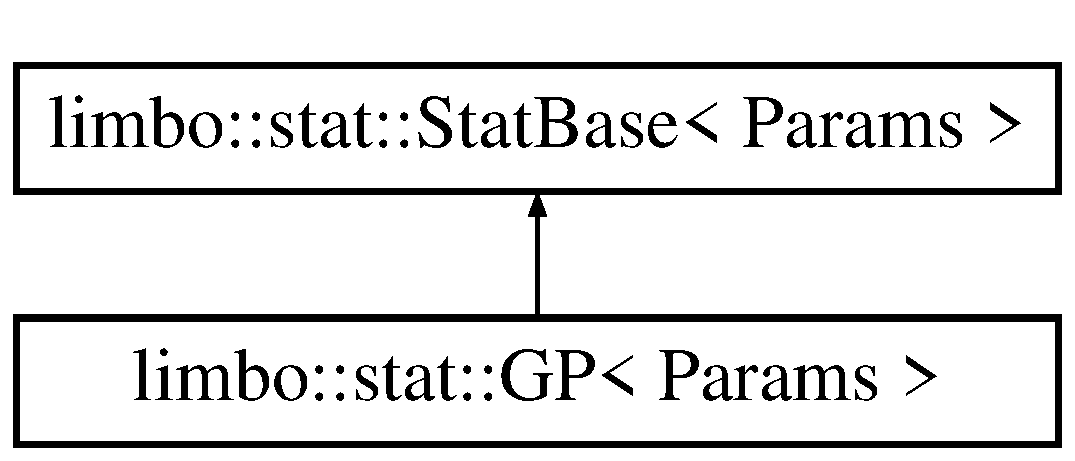
\includegraphics[height=2.000000cm]{structlimbo_1_1stat_1_1_g_p}
\end{center}
\end{figure}
\subsection*{Public Member Functions}
\begin{DoxyCompactItemize}
\item 
{\footnotesize template$<$typename B\+O , typename Aggregator\+Function $>$ }\\void \hyperlink{structlimbo_1_1stat_1_1_g_p_ae1af2dda46c2aaca5f757871b038694e}{operator()} (const B\+O \&bo, const Aggregator\+Function \&afun)
\end{DoxyCompactItemize}


\subsection{Detailed Description}
\subsubsection*{template$<$typename Params$>$struct limbo\+::stat\+::\+G\+P$<$ Params $>$}

filename\+: {\ttfamily gp\+\_\+$<$iteration$>$.dat} 

\subsection{Member Function Documentation}
\hypertarget{structlimbo_1_1stat_1_1_g_p_ae1af2dda46c2aaca5f757871b038694e}{}\index{limbo\+::stat\+::\+G\+P@{limbo\+::stat\+::\+G\+P}!operator()@{operator()}}
\index{operator()@{operator()}!limbo\+::stat\+::\+G\+P@{limbo\+::stat\+::\+G\+P}}
\subsubsection[{operator()}]{\setlength{\rightskip}{0pt plus 5cm}template$<$typename Params $>$ template$<$typename B\+O , typename Aggregator\+Function $>$ void {\bf limbo\+::stat\+::\+G\+P}$<$ Params $>$\+::operator() (
\begin{DoxyParamCaption}
\item[{const B\+O \&}]{bo, }
\item[{const Aggregator\+Function \&}]{afun}
\end{DoxyParamCaption}
)\hspace{0.3cm}{\ttfamily [inline]}}\label{structlimbo_1_1stat_1_1_g_p_ae1af2dda46c2aaca5f757871b038694e}


The documentation for this struct was generated from the following file\+:\begin{DoxyCompactItemize}
\item 
/tmp/doc\+\_\+limbo/limbo/src/limbo/stat/\hyperlink{stat_2gp_8hpp}{gp.\+hpp}\end{DoxyCompactItemize}

\hypertarget{classlimbo_1_1model_1_1_g_p}{}\section{limbo\+:\+:model\+:\+:GP$<$ Params, Kernel\+Function, Mean\+Function, Hyper\+Params\+Optimizer $>$ Class Template Reference}
\label{classlimbo_1_1model_1_1_g_p}\index{limbo\+::model\+::\+G\+P$<$ Params, Kernel\+Function, Mean\+Function, Hyper\+Params\+Optimizer $>$@{limbo\+::model\+::\+G\+P$<$ Params, Kernel\+Function, Mean\+Function, Hyper\+Params\+Optimizer $>$}}


{\ttfamily \#include $<$limbo/model/gp.\+hpp$>$}

\subsection*{Public Member Functions}
\begin{DoxyCompactItemize}
\item 
\hyperlink{classlimbo_1_1model_1_1_g_p_aa18de82f231f3aed6ce8cce4c778aedb}{GP} ()
\begin{DoxyCompactList}\small\item\em useful because the model might be created before knowing anything about the process \end{DoxyCompactList}\item 
\hyperlink{classlimbo_1_1model_1_1_g_p_ab36947c89e4f5ad92599656a21829755}{GP} (int \hyperlink{classlimbo_1_1model_1_1_g_p_a41d99e6a69d53fc7d9260d295f787bc3}{dim\+\_\+in}, int \hyperlink{classlimbo_1_1model_1_1_g_p_a077144695f9f0b33b64d4feb8fb4e447}{dim\+\_\+out})
\begin{DoxyCompactList}\small\item\em useful because the model might be created before having samples \end{DoxyCompactList}\item 
void \hyperlink{classlimbo_1_1model_1_1_g_p_a68bf0f4fdf3cfa5dd37e192e3cdf31c8}{compute} (const std\+::vector$<$ Eigen\+::\+Vector\+Xd $>$ \&\hyperlink{classlimbo_1_1model_1_1_g_p_abaa15a2e503bac670dd1a35fb377aa23}{samples}, const std\+::vector$<$ Eigen\+::\+Vector\+Xd $>$ \&observations, bool compute\+\_\+kernel=true)
\begin{DoxyCompactList}\small\item\em Compute the \hyperlink{classlimbo_1_1model_1_1_g_p}{GP} from samples and observations. This call needs to be explicit! \end{DoxyCompactList}\item 
void \hyperlink{classlimbo_1_1model_1_1_g_p_aa01b41e37de4def676cf6c79b08aac94}{optimize\+\_\+hyperparams} ()
\begin{DoxyCompactList}\small\item\em Do not forget to call this if you use hyper-\/prameters optimization!! \end{DoxyCompactList}\item 
void \hyperlink{classlimbo_1_1model_1_1_g_p_ae48c4db7c797a6844c18fdd7878a7b4b}{add\+\_\+sample} (const Eigen\+::\+Vector\+Xd \&sample, const Eigen\+::\+Vector\+Xd \&observation)
\item 
std\+::tuple$<$ Eigen\+::\+Vector\+Xd, double $>$ \hyperlink{classlimbo_1_1model_1_1_g_p_a33937ff7df97c01fdd9bf8911e0a6159}{query} (const Eigen\+::\+Vector\+Xd \&v) const 
\item 
Eigen\+::\+Vector\+Xd \hyperlink{classlimbo_1_1model_1_1_g_p_a5d26e30b8c53400cdf12058d83dc41f0}{mu} (const Eigen\+::\+Vector\+Xd \&v) const 
\item 
double \hyperlink{classlimbo_1_1model_1_1_g_p_a2ea153c1de2021740235cfa10822395d}{sigma} (const Eigen\+::\+Vector\+Xd \&v) const 
\item 
int \hyperlink{classlimbo_1_1model_1_1_g_p_a41d99e6a69d53fc7d9260d295f787bc3}{dim\+\_\+in} () const 
\begin{DoxyCompactList}\small\item\em return the number of dimensions of the input \end{DoxyCompactList}\item 
int \hyperlink{classlimbo_1_1model_1_1_g_p_a077144695f9f0b33b64d4feb8fb4e447}{dim\+\_\+out} () const 
\begin{DoxyCompactList}\small\item\em return the number of dimensions of the output \end{DoxyCompactList}\item 
const Kernel\+Function \& \hyperlink{classlimbo_1_1model_1_1_g_p_aaf794227fb4b8ba92bc22f15ec379d87}{kernel\+\_\+function} () const 
\item 
Kernel\+Function \& \hyperlink{classlimbo_1_1model_1_1_g_p_a442ffded72288fd9ea360ce1456f72a4}{kernel\+\_\+function} ()
\item 
const Mean\+Function \& \hyperlink{classlimbo_1_1model_1_1_g_p_a29be4dfec28fbf0ab970529a18a20c34}{mean\+\_\+function} () const 
\item 
Mean\+Function \& \hyperlink{classlimbo_1_1model_1_1_g_p_ad4a56a3630793def38840ea1c85c091e}{mean\+\_\+function} ()
\item 
Eigen\+::\+Vector\+Xd \hyperlink{classlimbo_1_1model_1_1_g_p_a480f1b249edf89bc6960512e8baceab8}{max\+\_\+observation} () const 
\begin{DoxyCompactList}\small\item\em return the maximum observation (only call this if the output of the \hyperlink{classlimbo_1_1model_1_1_g_p}{GP} is of dimension 1) \end{DoxyCompactList}\item 
Eigen\+::\+Vector\+Xd \hyperlink{classlimbo_1_1model_1_1_g_p_a802d8d4750626e6d38d83d36166000ac}{mean\+\_\+observation} () const 
\begin{DoxyCompactList}\small\item\em return the mean observation (only call this if the output of the \hyperlink{classlimbo_1_1model_1_1_g_p}{GP} is of dimension 1) \end{DoxyCompactList}\item 
const Eigen\+::\+Matrix\+Xd \& \hyperlink{classlimbo_1_1model_1_1_g_p_ade0d93b847e3d112735b3e8143470a55}{mean\+\_\+vector} () const 
\item 
const Eigen\+::\+Matrix\+Xd \& \hyperlink{classlimbo_1_1model_1_1_g_p_aa9d3799fdcd71a8ccc19bc43932fa321}{obs\+\_\+mean} () const 
\item 
int \hyperlink{classlimbo_1_1model_1_1_g_p_ac490915c95cc78f6cd836f78e3638bf1}{nb\+\_\+samples} () const 
\begin{DoxyCompactList}\small\item\em return the number of samples used to compute the \hyperlink{classlimbo_1_1model_1_1_g_p}{GP} \end{DoxyCompactList}\item 
void \hyperlink{classlimbo_1_1model_1_1_g_p_aff675b6136bdee1b907a1ca1c76699b4}{recompute} (bool update\+\_\+obs\+\_\+mean=true, bool update\+\_\+full\+\_\+kernel=true)
\begin{DoxyCompactList}\small\item\em recomputes the \hyperlink{classlimbo_1_1model_1_1_g_p}{GP} \end{DoxyCompactList}\item 
double \hyperlink{classlimbo_1_1model_1_1_g_p_a794ed0eeda29aaa7afe303b5e72d3927}{get\+\_\+lik} () const 
\begin{DoxyCompactList}\small\item\em return the likelihood (do not compute it!) \end{DoxyCompactList}\item 
void \hyperlink{classlimbo_1_1model_1_1_g_p_a4dfc1807eb4f113191dbd3ae51c053ee}{set\+\_\+lik} (const double \&lik)
\begin{DoxyCompactList}\small\item\em set the likelihood (you need to compute it from outside!) \end{DoxyCompactList}\item 
const Eigen\+::\+Matrix\+Xd \& \hyperlink{classlimbo_1_1model_1_1_g_p_a6f3a88531cc874a3a0cae0c218b0cf0a}{matrixL} () const 
\begin{DoxyCompactList}\small\item\em L\+LT matrix (from Cholesky decomposition) \end{DoxyCompactList}\item 
const Eigen\+::\+Matrix\+Xd \& \hyperlink{classlimbo_1_1model_1_1_g_p_adab606218ab9ef0c35babf8d1cc16d81}{alpha} () const 
\item 
const std\+::vector$<$ Eigen\+::\+Vector\+Xd $>$ \& \hyperlink{classlimbo_1_1model_1_1_g_p_abaa15a2e503bac670dd1a35fb377aa23}{samples} () const 
\begin{DoxyCompactList}\small\item\em return the list of samples that have been tested so far \end{DoxyCompactList}\end{DoxyCompactItemize}


\subsection{Detailed Description}
\subsubsection*{template$<$typename Params, typename Kernel\+Function, typename Mean\+Function, class Hyper\+Params\+Optimizer = gp\+::\+No\+L\+F\+Opt$<$\+Params$>$$>$\\*
class limbo\+::model\+::\+G\+P$<$ Params, Kernel\+Function, Mean\+Function, Hyper\+Params\+Optimizer $>$}

A classic Gaussian process. It is parametrized by\+:
\begin{DoxyItemize}
\item a mean function
\item \mbox{[}optionnal\mbox{]} an optimizer for the hyper-\/parameters 
\end{DoxyItemize}

\subsection{Constructor \& Destructor Documentation}
\index{limbo\+::model\+::\+GP@{limbo\+::model\+::\+GP}!GP@{GP}}
\index{GP@{GP}!limbo\+::model\+::\+GP@{limbo\+::model\+::\+GP}}
\subsubsection[{\texorpdfstring{G\+P()}{GP()}}]{\setlength{\rightskip}{0pt plus 5cm}template$<$typename Params , typename Kernel\+Function , typename Mean\+Function , class Hyper\+Params\+Optimizer  = gp\+::\+No\+L\+F\+Opt$<$\+Params$>$$>$ {\bf limbo\+::model\+::\+GP}$<$ Params, Kernel\+Function, Mean\+Function, Hyper\+Params\+Optimizer $>$\+::{\bf GP} (
\begin{DoxyParamCaption}
{}
\end{DoxyParamCaption}
)\hspace{0.3cm}{\ttfamily [inline]}}\hypertarget{classlimbo_1_1model_1_1_g_p_aa18de82f231f3aed6ce8cce4c778aedb}{}\label{classlimbo_1_1model_1_1_g_p_aa18de82f231f3aed6ce8cce4c778aedb}


useful because the model might be created before knowing anything about the process 

\index{limbo\+::model\+::\+GP@{limbo\+::model\+::\+GP}!GP@{GP}}
\index{GP@{GP}!limbo\+::model\+::\+GP@{limbo\+::model\+::\+GP}}
\subsubsection[{\texorpdfstring{G\+P(int dim\+\_\+in, int dim\+\_\+out)}{GP(int dim_in, int dim_out)}}]{\setlength{\rightskip}{0pt plus 5cm}template$<$typename Params , typename Kernel\+Function , typename Mean\+Function , class Hyper\+Params\+Optimizer  = gp\+::\+No\+L\+F\+Opt$<$\+Params$>$$>$ {\bf limbo\+::model\+::\+GP}$<$ Params, Kernel\+Function, Mean\+Function, Hyper\+Params\+Optimizer $>$\+::{\bf GP} (
\begin{DoxyParamCaption}
\item[{int}]{dim\+\_\+in, }
\item[{int}]{dim\+\_\+out}
\end{DoxyParamCaption}
)\hspace{0.3cm}{\ttfamily [inline]}}\hypertarget{classlimbo_1_1model_1_1_g_p_ab36947c89e4f5ad92599656a21829755}{}\label{classlimbo_1_1model_1_1_g_p_ab36947c89e4f5ad92599656a21829755}


useful because the model might be created before having samples 



\subsection{Member Function Documentation}
\index{limbo\+::model\+::\+GP@{limbo\+::model\+::\+GP}!add\+\_\+sample@{add\+\_\+sample}}
\index{add\+\_\+sample@{add\+\_\+sample}!limbo\+::model\+::\+GP@{limbo\+::model\+::\+GP}}
\subsubsection[{\texorpdfstring{add\+\_\+sample(const Eigen\+::\+Vector\+Xd \&sample, const Eigen\+::\+Vector\+Xd \&observation)}{add_sample(const Eigen::VectorXd &sample, const Eigen::VectorXd &observation)}}]{\setlength{\rightskip}{0pt plus 5cm}template$<$typename Params , typename Kernel\+Function , typename Mean\+Function , class Hyper\+Params\+Optimizer  = gp\+::\+No\+L\+F\+Opt$<$\+Params$>$$>$ void {\bf limbo\+::model\+::\+GP}$<$ Params, Kernel\+Function, Mean\+Function, Hyper\+Params\+Optimizer $>$\+::add\+\_\+sample (
\begin{DoxyParamCaption}
\item[{const Eigen\+::\+Vector\+Xd \&}]{sample, }
\item[{const Eigen\+::\+Vector\+Xd \&}]{observation}
\end{DoxyParamCaption}
)\hspace{0.3cm}{\ttfamily [inline]}}\hypertarget{classlimbo_1_1model_1_1_g_p_ae48c4db7c797a6844c18fdd7878a7b4b}{}\label{classlimbo_1_1model_1_1_g_p_ae48c4db7c797a6844c18fdd7878a7b4b}
add sample and update the \hyperlink{classlimbo_1_1model_1_1_g_p}{GP}. This code uses an incremental implementation of the Cholesky decomposition. It is therefore much faster than a call to \hyperlink{classlimbo_1_1model_1_1_g_p_a68bf0f4fdf3cfa5dd37e192e3cdf31c8}{compute()} \index{limbo\+::model\+::\+GP@{limbo\+::model\+::\+GP}!alpha@{alpha}}
\index{alpha@{alpha}!limbo\+::model\+::\+GP@{limbo\+::model\+::\+GP}}
\subsubsection[{\texorpdfstring{alpha() const }{alpha() const }}]{\setlength{\rightskip}{0pt plus 5cm}template$<$typename Params , typename Kernel\+Function , typename Mean\+Function , class Hyper\+Params\+Optimizer  = gp\+::\+No\+L\+F\+Opt$<$\+Params$>$$>$ const Eigen\+::\+Matrix\+Xd\& {\bf limbo\+::model\+::\+GP}$<$ Params, Kernel\+Function, Mean\+Function, Hyper\+Params\+Optimizer $>$\+::alpha (
\begin{DoxyParamCaption}
{}
\end{DoxyParamCaption}
) const\hspace{0.3cm}{\ttfamily [inline]}}\hypertarget{classlimbo_1_1model_1_1_g_p_adab606218ab9ef0c35babf8d1cc16d81}{}\label{classlimbo_1_1model_1_1_g_p_adab606218ab9ef0c35babf8d1cc16d81}
\index{limbo\+::model\+::\+GP@{limbo\+::model\+::\+GP}!compute@{compute}}
\index{compute@{compute}!limbo\+::model\+::\+GP@{limbo\+::model\+::\+GP}}
\subsubsection[{\texorpdfstring{compute(const std\+::vector$<$ Eigen\+::\+Vector\+Xd $>$ \&samples, const std\+::vector$<$ Eigen\+::\+Vector\+Xd $>$ \&observations, bool compute\+\_\+kernel=true)}{compute(const std::vector< Eigen::VectorXd > &samples, const std::vector< Eigen::VectorXd > &observations, bool compute_kernel=true)}}]{\setlength{\rightskip}{0pt plus 5cm}template$<$typename Params , typename Kernel\+Function , typename Mean\+Function , class Hyper\+Params\+Optimizer  = gp\+::\+No\+L\+F\+Opt$<$\+Params$>$$>$ void {\bf limbo\+::model\+::\+GP}$<$ Params, Kernel\+Function, Mean\+Function, Hyper\+Params\+Optimizer $>$\+::compute (
\begin{DoxyParamCaption}
\item[{const std\+::vector$<$ Eigen\+::\+Vector\+Xd $>$ \&}]{samples, }
\item[{const std\+::vector$<$ Eigen\+::\+Vector\+Xd $>$ \&}]{observations, }
\item[{bool}]{compute\+\_\+kernel = {\ttfamily true}}
\end{DoxyParamCaption}
)\hspace{0.3cm}{\ttfamily [inline]}}\hypertarget{classlimbo_1_1model_1_1_g_p_a68bf0f4fdf3cfa5dd37e192e3cdf31c8}{}\label{classlimbo_1_1model_1_1_g_p_a68bf0f4fdf3cfa5dd37e192e3cdf31c8}


Compute the \hyperlink{classlimbo_1_1model_1_1_g_p}{GP} from samples and observations. This call needs to be explicit! 

\index{limbo\+::model\+::\+GP@{limbo\+::model\+::\+GP}!dim\+\_\+in@{dim\+\_\+in}}
\index{dim\+\_\+in@{dim\+\_\+in}!limbo\+::model\+::\+GP@{limbo\+::model\+::\+GP}}
\subsubsection[{\texorpdfstring{dim\+\_\+in() const }{dim_in() const }}]{\setlength{\rightskip}{0pt plus 5cm}template$<$typename Params , typename Kernel\+Function , typename Mean\+Function , class Hyper\+Params\+Optimizer  = gp\+::\+No\+L\+F\+Opt$<$\+Params$>$$>$ int {\bf limbo\+::model\+::\+GP}$<$ Params, Kernel\+Function, Mean\+Function, Hyper\+Params\+Optimizer $>$\+::dim\+\_\+in (
\begin{DoxyParamCaption}
{}
\end{DoxyParamCaption}
) const\hspace{0.3cm}{\ttfamily [inline]}}\hypertarget{classlimbo_1_1model_1_1_g_p_a41d99e6a69d53fc7d9260d295f787bc3}{}\label{classlimbo_1_1model_1_1_g_p_a41d99e6a69d53fc7d9260d295f787bc3}


return the number of dimensions of the input 

\index{limbo\+::model\+::\+GP@{limbo\+::model\+::\+GP}!dim\+\_\+out@{dim\+\_\+out}}
\index{dim\+\_\+out@{dim\+\_\+out}!limbo\+::model\+::\+GP@{limbo\+::model\+::\+GP}}
\subsubsection[{\texorpdfstring{dim\+\_\+out() const }{dim_out() const }}]{\setlength{\rightskip}{0pt plus 5cm}template$<$typename Params , typename Kernel\+Function , typename Mean\+Function , class Hyper\+Params\+Optimizer  = gp\+::\+No\+L\+F\+Opt$<$\+Params$>$$>$ int {\bf limbo\+::model\+::\+GP}$<$ Params, Kernel\+Function, Mean\+Function, Hyper\+Params\+Optimizer $>$\+::dim\+\_\+out (
\begin{DoxyParamCaption}
{}
\end{DoxyParamCaption}
) const\hspace{0.3cm}{\ttfamily [inline]}}\hypertarget{classlimbo_1_1model_1_1_g_p_a077144695f9f0b33b64d4feb8fb4e447}{}\label{classlimbo_1_1model_1_1_g_p_a077144695f9f0b33b64d4feb8fb4e447}


return the number of dimensions of the output 

\index{limbo\+::model\+::\+GP@{limbo\+::model\+::\+GP}!get\+\_\+lik@{get\+\_\+lik}}
\index{get\+\_\+lik@{get\+\_\+lik}!limbo\+::model\+::\+GP@{limbo\+::model\+::\+GP}}
\subsubsection[{\texorpdfstring{get\+\_\+lik() const }{get_lik() const }}]{\setlength{\rightskip}{0pt plus 5cm}template$<$typename Params , typename Kernel\+Function , typename Mean\+Function , class Hyper\+Params\+Optimizer  = gp\+::\+No\+L\+F\+Opt$<$\+Params$>$$>$ double {\bf limbo\+::model\+::\+GP}$<$ Params, Kernel\+Function, Mean\+Function, Hyper\+Params\+Optimizer $>$\+::get\+\_\+lik (
\begin{DoxyParamCaption}
{}
\end{DoxyParamCaption}
) const\hspace{0.3cm}{\ttfamily [inline]}}\hypertarget{classlimbo_1_1model_1_1_g_p_a794ed0eeda29aaa7afe303b5e72d3927}{}\label{classlimbo_1_1model_1_1_g_p_a794ed0eeda29aaa7afe303b5e72d3927}


return the likelihood (do not compute it!) 

\index{limbo\+::model\+::\+GP@{limbo\+::model\+::\+GP}!kernel\+\_\+function@{kernel\+\_\+function}}
\index{kernel\+\_\+function@{kernel\+\_\+function}!limbo\+::model\+::\+GP@{limbo\+::model\+::\+GP}}
\subsubsection[{\texorpdfstring{kernel\+\_\+function() const }{kernel_function() const }}]{\setlength{\rightskip}{0pt plus 5cm}template$<$typename Params , typename Kernel\+Function , typename Mean\+Function , class Hyper\+Params\+Optimizer  = gp\+::\+No\+L\+F\+Opt$<$\+Params$>$$>$ const Kernel\+Function\& {\bf limbo\+::model\+::\+GP}$<$ Params, Kernel\+Function, Mean\+Function, Hyper\+Params\+Optimizer $>$\+::kernel\+\_\+function (
\begin{DoxyParamCaption}
{}
\end{DoxyParamCaption}
) const\hspace{0.3cm}{\ttfamily [inline]}}\hypertarget{classlimbo_1_1model_1_1_g_p_aaf794227fb4b8ba92bc22f15ec379d87}{}\label{classlimbo_1_1model_1_1_g_p_aaf794227fb4b8ba92bc22f15ec379d87}
\index{limbo\+::model\+::\+GP@{limbo\+::model\+::\+GP}!kernel\+\_\+function@{kernel\+\_\+function}}
\index{kernel\+\_\+function@{kernel\+\_\+function}!limbo\+::model\+::\+GP@{limbo\+::model\+::\+GP}}
\subsubsection[{\texorpdfstring{kernel\+\_\+function()}{kernel_function()}}]{\setlength{\rightskip}{0pt plus 5cm}template$<$typename Params , typename Kernel\+Function , typename Mean\+Function , class Hyper\+Params\+Optimizer  = gp\+::\+No\+L\+F\+Opt$<$\+Params$>$$>$ Kernel\+Function\& {\bf limbo\+::model\+::\+GP}$<$ Params, Kernel\+Function, Mean\+Function, Hyper\+Params\+Optimizer $>$\+::kernel\+\_\+function (
\begin{DoxyParamCaption}
{}
\end{DoxyParamCaption}
)\hspace{0.3cm}{\ttfamily [inline]}}\hypertarget{classlimbo_1_1model_1_1_g_p_a442ffded72288fd9ea360ce1456f72a4}{}\label{classlimbo_1_1model_1_1_g_p_a442ffded72288fd9ea360ce1456f72a4}
\index{limbo\+::model\+::\+GP@{limbo\+::model\+::\+GP}!matrixL@{matrixL}}
\index{matrixL@{matrixL}!limbo\+::model\+::\+GP@{limbo\+::model\+::\+GP}}
\subsubsection[{\texorpdfstring{matrix\+L() const }{matrixL() const }}]{\setlength{\rightskip}{0pt plus 5cm}template$<$typename Params , typename Kernel\+Function , typename Mean\+Function , class Hyper\+Params\+Optimizer  = gp\+::\+No\+L\+F\+Opt$<$\+Params$>$$>$ const Eigen\+::\+Matrix\+Xd\& {\bf limbo\+::model\+::\+GP}$<$ Params, Kernel\+Function, Mean\+Function, Hyper\+Params\+Optimizer $>$\+::matrixL (
\begin{DoxyParamCaption}
{}
\end{DoxyParamCaption}
) const\hspace{0.3cm}{\ttfamily [inline]}}\hypertarget{classlimbo_1_1model_1_1_g_p_a6f3a88531cc874a3a0cae0c218b0cf0a}{}\label{classlimbo_1_1model_1_1_g_p_a6f3a88531cc874a3a0cae0c218b0cf0a}


L\+LT matrix (from Cholesky decomposition) 

\index{limbo\+::model\+::\+GP@{limbo\+::model\+::\+GP}!max\+\_\+observation@{max\+\_\+observation}}
\index{max\+\_\+observation@{max\+\_\+observation}!limbo\+::model\+::\+GP@{limbo\+::model\+::\+GP}}
\subsubsection[{\texorpdfstring{max\+\_\+observation() const }{max_observation() const }}]{\setlength{\rightskip}{0pt plus 5cm}template$<$typename Params , typename Kernel\+Function , typename Mean\+Function , class Hyper\+Params\+Optimizer  = gp\+::\+No\+L\+F\+Opt$<$\+Params$>$$>$ Eigen\+::\+Vector\+Xd {\bf limbo\+::model\+::\+GP}$<$ Params, Kernel\+Function, Mean\+Function, Hyper\+Params\+Optimizer $>$\+::max\+\_\+observation (
\begin{DoxyParamCaption}
{}
\end{DoxyParamCaption}
) const\hspace{0.3cm}{\ttfamily [inline]}}\hypertarget{classlimbo_1_1model_1_1_g_p_a480f1b249edf89bc6960512e8baceab8}{}\label{classlimbo_1_1model_1_1_g_p_a480f1b249edf89bc6960512e8baceab8}


return the maximum observation (only call this if the output of the \hyperlink{classlimbo_1_1model_1_1_g_p}{GP} is of dimension 1) 

\index{limbo\+::model\+::\+GP@{limbo\+::model\+::\+GP}!mean\+\_\+function@{mean\+\_\+function}}
\index{mean\+\_\+function@{mean\+\_\+function}!limbo\+::model\+::\+GP@{limbo\+::model\+::\+GP}}
\subsubsection[{\texorpdfstring{mean\+\_\+function() const }{mean_function() const }}]{\setlength{\rightskip}{0pt plus 5cm}template$<$typename Params , typename Kernel\+Function , typename Mean\+Function , class Hyper\+Params\+Optimizer  = gp\+::\+No\+L\+F\+Opt$<$\+Params$>$$>$ const Mean\+Function\& {\bf limbo\+::model\+::\+GP}$<$ Params, Kernel\+Function, Mean\+Function, Hyper\+Params\+Optimizer $>$\+::mean\+\_\+function (
\begin{DoxyParamCaption}
{}
\end{DoxyParamCaption}
) const\hspace{0.3cm}{\ttfamily [inline]}}\hypertarget{classlimbo_1_1model_1_1_g_p_a29be4dfec28fbf0ab970529a18a20c34}{}\label{classlimbo_1_1model_1_1_g_p_a29be4dfec28fbf0ab970529a18a20c34}
\index{limbo\+::model\+::\+GP@{limbo\+::model\+::\+GP}!mean\+\_\+function@{mean\+\_\+function}}
\index{mean\+\_\+function@{mean\+\_\+function}!limbo\+::model\+::\+GP@{limbo\+::model\+::\+GP}}
\subsubsection[{\texorpdfstring{mean\+\_\+function()}{mean_function()}}]{\setlength{\rightskip}{0pt plus 5cm}template$<$typename Params , typename Kernel\+Function , typename Mean\+Function , class Hyper\+Params\+Optimizer  = gp\+::\+No\+L\+F\+Opt$<$\+Params$>$$>$ Mean\+Function\& {\bf limbo\+::model\+::\+GP}$<$ Params, Kernel\+Function, Mean\+Function, Hyper\+Params\+Optimizer $>$\+::mean\+\_\+function (
\begin{DoxyParamCaption}
{}
\end{DoxyParamCaption}
)\hspace{0.3cm}{\ttfamily [inline]}}\hypertarget{classlimbo_1_1model_1_1_g_p_ad4a56a3630793def38840ea1c85c091e}{}\label{classlimbo_1_1model_1_1_g_p_ad4a56a3630793def38840ea1c85c091e}
\index{limbo\+::model\+::\+GP@{limbo\+::model\+::\+GP}!mean\+\_\+observation@{mean\+\_\+observation}}
\index{mean\+\_\+observation@{mean\+\_\+observation}!limbo\+::model\+::\+GP@{limbo\+::model\+::\+GP}}
\subsubsection[{\texorpdfstring{mean\+\_\+observation() const }{mean_observation() const }}]{\setlength{\rightskip}{0pt plus 5cm}template$<$typename Params , typename Kernel\+Function , typename Mean\+Function , class Hyper\+Params\+Optimizer  = gp\+::\+No\+L\+F\+Opt$<$\+Params$>$$>$ Eigen\+::\+Vector\+Xd {\bf limbo\+::model\+::\+GP}$<$ Params, Kernel\+Function, Mean\+Function, Hyper\+Params\+Optimizer $>$\+::mean\+\_\+observation (
\begin{DoxyParamCaption}
{}
\end{DoxyParamCaption}
) const\hspace{0.3cm}{\ttfamily [inline]}}\hypertarget{classlimbo_1_1model_1_1_g_p_a802d8d4750626e6d38d83d36166000ac}{}\label{classlimbo_1_1model_1_1_g_p_a802d8d4750626e6d38d83d36166000ac}


return the mean observation (only call this if the output of the \hyperlink{classlimbo_1_1model_1_1_g_p}{GP} is of dimension 1) 

\index{limbo\+::model\+::\+GP@{limbo\+::model\+::\+GP}!mean\+\_\+vector@{mean\+\_\+vector}}
\index{mean\+\_\+vector@{mean\+\_\+vector}!limbo\+::model\+::\+GP@{limbo\+::model\+::\+GP}}
\subsubsection[{\texorpdfstring{mean\+\_\+vector() const }{mean_vector() const }}]{\setlength{\rightskip}{0pt plus 5cm}template$<$typename Params , typename Kernel\+Function , typename Mean\+Function , class Hyper\+Params\+Optimizer  = gp\+::\+No\+L\+F\+Opt$<$\+Params$>$$>$ const Eigen\+::\+Matrix\+Xd\& {\bf limbo\+::model\+::\+GP}$<$ Params, Kernel\+Function, Mean\+Function, Hyper\+Params\+Optimizer $>$\+::mean\+\_\+vector (
\begin{DoxyParamCaption}
{}
\end{DoxyParamCaption}
) const\hspace{0.3cm}{\ttfamily [inline]}}\hypertarget{classlimbo_1_1model_1_1_g_p_ade0d93b847e3d112735b3e8143470a55}{}\label{classlimbo_1_1model_1_1_g_p_ade0d93b847e3d112735b3e8143470a55}
\index{limbo\+::model\+::\+GP@{limbo\+::model\+::\+GP}!mu@{mu}}
\index{mu@{mu}!limbo\+::model\+::\+GP@{limbo\+::model\+::\+GP}}
\subsubsection[{\texorpdfstring{mu(const Eigen\+::\+Vector\+Xd \&v) const }{mu(const Eigen::VectorXd &v) const }}]{\setlength{\rightskip}{0pt plus 5cm}template$<$typename Params , typename Kernel\+Function , typename Mean\+Function , class Hyper\+Params\+Optimizer  = gp\+::\+No\+L\+F\+Opt$<$\+Params$>$$>$ Eigen\+::\+Vector\+Xd {\bf limbo\+::model\+::\+GP}$<$ Params, Kernel\+Function, Mean\+Function, Hyper\+Params\+Optimizer $>$\+::mu (
\begin{DoxyParamCaption}
\item[{const Eigen\+::\+Vector\+Xd \&}]{v}
\end{DoxyParamCaption}
) const\hspace{0.3cm}{\ttfamily [inline]}}\hypertarget{classlimbo_1_1model_1_1_g_p_a5d26e30b8c53400cdf12058d83dc41f0}{}\label{classlimbo_1_1model_1_1_g_p_a5d26e30b8c53400cdf12058d83dc41f0}
\textbackslash{}rst return \+:math\+:{\ttfamily \textbackslash{}mu} (unormalized). If there is no sample, return the value according to the mean function. \textbackslash{}endrst \index{limbo\+::model\+::\+GP@{limbo\+::model\+::\+GP}!nb\+\_\+samples@{nb\+\_\+samples}}
\index{nb\+\_\+samples@{nb\+\_\+samples}!limbo\+::model\+::\+GP@{limbo\+::model\+::\+GP}}
\subsubsection[{\texorpdfstring{nb\+\_\+samples() const }{nb_samples() const }}]{\setlength{\rightskip}{0pt plus 5cm}template$<$typename Params , typename Kernel\+Function , typename Mean\+Function , class Hyper\+Params\+Optimizer  = gp\+::\+No\+L\+F\+Opt$<$\+Params$>$$>$ int {\bf limbo\+::model\+::\+GP}$<$ Params, Kernel\+Function, Mean\+Function, Hyper\+Params\+Optimizer $>$\+::nb\+\_\+samples (
\begin{DoxyParamCaption}
{}
\end{DoxyParamCaption}
) const\hspace{0.3cm}{\ttfamily [inline]}}\hypertarget{classlimbo_1_1model_1_1_g_p_ac490915c95cc78f6cd836f78e3638bf1}{}\label{classlimbo_1_1model_1_1_g_p_ac490915c95cc78f6cd836f78e3638bf1}


return the number of samples used to compute the \hyperlink{classlimbo_1_1model_1_1_g_p}{GP} 

\index{limbo\+::model\+::\+GP@{limbo\+::model\+::\+GP}!obs\+\_\+mean@{obs\+\_\+mean}}
\index{obs\+\_\+mean@{obs\+\_\+mean}!limbo\+::model\+::\+GP@{limbo\+::model\+::\+GP}}
\subsubsection[{\texorpdfstring{obs\+\_\+mean() const }{obs_mean() const }}]{\setlength{\rightskip}{0pt plus 5cm}template$<$typename Params , typename Kernel\+Function , typename Mean\+Function , class Hyper\+Params\+Optimizer  = gp\+::\+No\+L\+F\+Opt$<$\+Params$>$$>$ const Eigen\+::\+Matrix\+Xd\& {\bf limbo\+::model\+::\+GP}$<$ Params, Kernel\+Function, Mean\+Function, Hyper\+Params\+Optimizer $>$\+::obs\+\_\+mean (
\begin{DoxyParamCaption}
{}
\end{DoxyParamCaption}
) const\hspace{0.3cm}{\ttfamily [inline]}}\hypertarget{classlimbo_1_1model_1_1_g_p_aa9d3799fdcd71a8ccc19bc43932fa321}{}\label{classlimbo_1_1model_1_1_g_p_aa9d3799fdcd71a8ccc19bc43932fa321}
\index{limbo\+::model\+::\+GP@{limbo\+::model\+::\+GP}!optimize\+\_\+hyperparams@{optimize\+\_\+hyperparams}}
\index{optimize\+\_\+hyperparams@{optimize\+\_\+hyperparams}!limbo\+::model\+::\+GP@{limbo\+::model\+::\+GP}}
\subsubsection[{\texorpdfstring{optimize\+\_\+hyperparams()}{optimize_hyperparams()}}]{\setlength{\rightskip}{0pt plus 5cm}template$<$typename Params , typename Kernel\+Function , typename Mean\+Function , class Hyper\+Params\+Optimizer  = gp\+::\+No\+L\+F\+Opt$<$\+Params$>$$>$ void {\bf limbo\+::model\+::\+GP}$<$ Params, Kernel\+Function, Mean\+Function, Hyper\+Params\+Optimizer $>$\+::optimize\+\_\+hyperparams (
\begin{DoxyParamCaption}
{}
\end{DoxyParamCaption}
)\hspace{0.3cm}{\ttfamily [inline]}}\hypertarget{classlimbo_1_1model_1_1_g_p_aa01b41e37de4def676cf6c79b08aac94}{}\label{classlimbo_1_1model_1_1_g_p_aa01b41e37de4def676cf6c79b08aac94}


Do not forget to call this if you use hyper-\/prameters optimization!! 

\index{limbo\+::model\+::\+GP@{limbo\+::model\+::\+GP}!query@{query}}
\index{query@{query}!limbo\+::model\+::\+GP@{limbo\+::model\+::\+GP}}
\subsubsection[{\texorpdfstring{query(const Eigen\+::\+Vector\+Xd \&v) const }{query(const Eigen::VectorXd &v) const }}]{\setlength{\rightskip}{0pt plus 5cm}template$<$typename Params , typename Kernel\+Function , typename Mean\+Function , class Hyper\+Params\+Optimizer  = gp\+::\+No\+L\+F\+Opt$<$\+Params$>$$>$ std\+::tuple$<$Eigen\+::\+Vector\+Xd, double$>$ {\bf limbo\+::model\+::\+GP}$<$ Params, Kernel\+Function, Mean\+Function, Hyper\+Params\+Optimizer $>$\+::query (
\begin{DoxyParamCaption}
\item[{const Eigen\+::\+Vector\+Xd \&}]{v}
\end{DoxyParamCaption}
) const\hspace{0.3cm}{\ttfamily [inline]}}\hypertarget{classlimbo_1_1model_1_1_g_p_a33937ff7df97c01fdd9bf8911e0a6159}{}\label{classlimbo_1_1model_1_1_g_p_a33937ff7df97c01fdd9bf8911e0a6159}
\textbackslash{}rst return \+:math\+:{\ttfamily \textbackslash{}mu}, \+:math\+:{\ttfamily \textbackslash{}sigma$^\wedge$2} (unormalized). If there is no sample, return the value according to the mean function. Using this method instead of separate calls to \hyperlink{classlimbo_1_1model_1_1_g_p_a5d26e30b8c53400cdf12058d83dc41f0}{mu()} and \hyperlink{classlimbo_1_1model_1_1_g_p_a2ea153c1de2021740235cfa10822395d}{sigma()} is more efficient because some computations are shared between \hyperlink{classlimbo_1_1model_1_1_g_p_a5d26e30b8c53400cdf12058d83dc41f0}{mu()} and \hyperlink{classlimbo_1_1model_1_1_g_p_a2ea153c1de2021740235cfa10822395d}{sigma()}. \textbackslash{}endrst \index{limbo\+::model\+::\+GP@{limbo\+::model\+::\+GP}!recompute@{recompute}}
\index{recompute@{recompute}!limbo\+::model\+::\+GP@{limbo\+::model\+::\+GP}}
\subsubsection[{\texorpdfstring{recompute(bool update\+\_\+obs\+\_\+mean=true, bool update\+\_\+full\+\_\+kernel=true)}{recompute(bool update_obs_mean=true, bool update_full_kernel=true)}}]{\setlength{\rightskip}{0pt plus 5cm}template$<$typename Params , typename Kernel\+Function , typename Mean\+Function , class Hyper\+Params\+Optimizer  = gp\+::\+No\+L\+F\+Opt$<$\+Params$>$$>$ void {\bf limbo\+::model\+::\+GP}$<$ Params, Kernel\+Function, Mean\+Function, Hyper\+Params\+Optimizer $>$\+::recompute (
\begin{DoxyParamCaption}
\item[{bool}]{update\+\_\+obs\+\_\+mean = {\ttfamily true}, }
\item[{bool}]{update\+\_\+full\+\_\+kernel = {\ttfamily true}}
\end{DoxyParamCaption}
)\hspace{0.3cm}{\ttfamily [inline]}}\hypertarget{classlimbo_1_1model_1_1_g_p_aff675b6136bdee1b907a1ca1c76699b4}{}\label{classlimbo_1_1model_1_1_g_p_aff675b6136bdee1b907a1ca1c76699b4}


recomputes the \hyperlink{classlimbo_1_1model_1_1_g_p}{GP} 

\index{limbo\+::model\+::\+GP@{limbo\+::model\+::\+GP}!samples@{samples}}
\index{samples@{samples}!limbo\+::model\+::\+GP@{limbo\+::model\+::\+GP}}
\subsubsection[{\texorpdfstring{samples() const }{samples() const }}]{\setlength{\rightskip}{0pt plus 5cm}template$<$typename Params , typename Kernel\+Function , typename Mean\+Function , class Hyper\+Params\+Optimizer  = gp\+::\+No\+L\+F\+Opt$<$\+Params$>$$>$ const std\+::vector$<$Eigen\+::\+Vector\+Xd$>$\& {\bf limbo\+::model\+::\+GP}$<$ Params, Kernel\+Function, Mean\+Function, Hyper\+Params\+Optimizer $>$\+::samples (
\begin{DoxyParamCaption}
{}
\end{DoxyParamCaption}
) const\hspace{0.3cm}{\ttfamily [inline]}}\hypertarget{classlimbo_1_1model_1_1_g_p_abaa15a2e503bac670dd1a35fb377aa23}{}\label{classlimbo_1_1model_1_1_g_p_abaa15a2e503bac670dd1a35fb377aa23}


return the list of samples that have been tested so far 

\index{limbo\+::model\+::\+GP@{limbo\+::model\+::\+GP}!set\+\_\+lik@{set\+\_\+lik}}
\index{set\+\_\+lik@{set\+\_\+lik}!limbo\+::model\+::\+GP@{limbo\+::model\+::\+GP}}
\subsubsection[{\texorpdfstring{set\+\_\+lik(const double \&lik)}{set_lik(const double &lik)}}]{\setlength{\rightskip}{0pt plus 5cm}template$<$typename Params , typename Kernel\+Function , typename Mean\+Function , class Hyper\+Params\+Optimizer  = gp\+::\+No\+L\+F\+Opt$<$\+Params$>$$>$ void {\bf limbo\+::model\+::\+GP}$<$ Params, Kernel\+Function, Mean\+Function, Hyper\+Params\+Optimizer $>$\+::set\+\_\+lik (
\begin{DoxyParamCaption}
\item[{const double \&}]{lik}
\end{DoxyParamCaption}
)\hspace{0.3cm}{\ttfamily [inline]}}\hypertarget{classlimbo_1_1model_1_1_g_p_a4dfc1807eb4f113191dbd3ae51c053ee}{}\label{classlimbo_1_1model_1_1_g_p_a4dfc1807eb4f113191dbd3ae51c053ee}


set the likelihood (you need to compute it from outside!) 

\index{limbo\+::model\+::\+GP@{limbo\+::model\+::\+GP}!sigma@{sigma}}
\index{sigma@{sigma}!limbo\+::model\+::\+GP@{limbo\+::model\+::\+GP}}
\subsubsection[{\texorpdfstring{sigma(const Eigen\+::\+Vector\+Xd \&v) const }{sigma(const Eigen::VectorXd &v) const }}]{\setlength{\rightskip}{0pt plus 5cm}template$<$typename Params , typename Kernel\+Function , typename Mean\+Function , class Hyper\+Params\+Optimizer  = gp\+::\+No\+L\+F\+Opt$<$\+Params$>$$>$ double {\bf limbo\+::model\+::\+GP}$<$ Params, Kernel\+Function, Mean\+Function, Hyper\+Params\+Optimizer $>$\+::sigma (
\begin{DoxyParamCaption}
\item[{const Eigen\+::\+Vector\+Xd \&}]{v}
\end{DoxyParamCaption}
) const\hspace{0.3cm}{\ttfamily [inline]}}\hypertarget{classlimbo_1_1model_1_1_g_p_a2ea153c1de2021740235cfa10822395d}{}\label{classlimbo_1_1model_1_1_g_p_a2ea153c1de2021740235cfa10822395d}
\textbackslash{}rst return \+:math\+:{\ttfamily \textbackslash{}sigma$^\wedge$2} (unormalized). If there is no sample, return the max \+:math\+:{\ttfamily \textbackslash{}sigma$^\wedge$2}. \textbackslash{}endrst 

The documentation for this class was generated from the following file\+:\begin{DoxyCompactItemize}
\item 
/tmp/doc\+\_\+limbo/limbo/src/limbo/model/\hyperlink{model_2gp_8hpp}{gp.\+hpp}\end{DoxyCompactItemize}

\hypertarget{classlimbo_1_1acqui_1_1_g_p___u_c_b}{}\section{limbo\+:\+:acqui\+:\+:G\+P\+\_\+\+U\+CB$<$ Params, Model $>$ Class Template Reference}
\label{classlimbo_1_1acqui_1_1_g_p___u_c_b}\index{limbo\+::acqui\+::\+G\+P\+\_\+\+U\+C\+B$<$ Params, Model $>$@{limbo\+::acqui\+::\+G\+P\+\_\+\+U\+C\+B$<$ Params, Model $>$}}


{\ttfamily \#include $<$limbo/acqui/gp\+\_\+ucb.\+hpp$>$}

\subsection*{Public Member Functions}
\begin{DoxyCompactItemize}
\item 
\hyperlink{classlimbo_1_1acqui_1_1_g_p___u_c_b_a9846faaa39b1d1d7b039284f2c905205}{G\+P\+\_\+\+U\+CB} (const Model \&model, int iteration)
\item 
size\+\_\+t \hyperlink{classlimbo_1_1acqui_1_1_g_p___u_c_b_a30c58b2f857da76de61e8cf555e73d06}{dim\+\_\+in} () const 
\item 
size\+\_\+t \hyperlink{classlimbo_1_1acqui_1_1_g_p___u_c_b_abde3ddcfa0bfb16d453587832f4e78b1}{dim\+\_\+out} () const 
\item 
{\footnotesize template$<$typename Aggregator\+Function $>$ }\\\hyperlink{group__opt__tools_ga362b55973a38ac71f27a06f9d9c14f24}{opt\+::eval\+\_\+t} \hyperlink{classlimbo_1_1acqui_1_1_g_p___u_c_b_a81dbe2aae8aea9d463547ac4d9236741}{operator()} (const Eigen\+::\+Vector\+Xd \&v, const Aggregator\+Function \&afun, bool gradient) const 
\end{DoxyCompactItemize}


\subsection{Detailed Description}
\subsubsection*{template$<$typename Params, typename Model$>$\\*
class limbo\+::acqui\+::\+G\+P\+\_\+\+U\+C\+B$<$ Params, Model $>$}

\begin{DoxyVerb}embed:rst
GP-UCB (Upper Confidence Bound). See :cite:`brochu2010tutorial`, p. 15. See also: http://arxiv.org/abs/0912.3995

.. math::
  UCB(x) = \mu(x) + \kappa \sigma(x).

with:

.. math::
  \kappa = \sqrt{2 \log{(\frac{n^{D/2+2}\pi^2}{3 \delta})}}

where :math:`n` is the number of past evaluations of the objective function and :math:`D` the dimensionality of the parameters (dim_in).

Parameters:
  - `double delta` (a small number in [0,1], e.g. 0.1)
\end{DoxyVerb}
 

\subsection{Constructor \& Destructor Documentation}
\index{limbo\+::acqui\+::\+G\+P\+\_\+\+U\+CB@{limbo\+::acqui\+::\+G\+P\+\_\+\+U\+CB}!G\+P\+\_\+\+U\+CB@{G\+P\+\_\+\+U\+CB}}
\index{G\+P\+\_\+\+U\+CB@{G\+P\+\_\+\+U\+CB}!limbo\+::acqui\+::\+G\+P\+\_\+\+U\+CB@{limbo\+::acqui\+::\+G\+P\+\_\+\+U\+CB}}
\subsubsection[{\texorpdfstring{G\+P\+\_\+\+U\+C\+B(const Model \&model, int iteration)}{GP_UCB(const Model &model, int iteration)}}]{\setlength{\rightskip}{0pt plus 5cm}template$<$typename Params , typename Model $>$ {\bf limbo\+::acqui\+::\+G\+P\+\_\+\+U\+CB}$<$ Params, Model $>$\+::{\bf G\+P\+\_\+\+U\+CB} (
\begin{DoxyParamCaption}
\item[{const Model \&}]{model, }
\item[{int}]{iteration}
\end{DoxyParamCaption}
)\hspace{0.3cm}{\ttfamily [inline]}}\hypertarget{classlimbo_1_1acqui_1_1_g_p___u_c_b_a9846faaa39b1d1d7b039284f2c905205}{}\label{classlimbo_1_1acqui_1_1_g_p___u_c_b_a9846faaa39b1d1d7b039284f2c905205}


\subsection{Member Function Documentation}
\index{limbo\+::acqui\+::\+G\+P\+\_\+\+U\+CB@{limbo\+::acqui\+::\+G\+P\+\_\+\+U\+CB}!dim\+\_\+in@{dim\+\_\+in}}
\index{dim\+\_\+in@{dim\+\_\+in}!limbo\+::acqui\+::\+G\+P\+\_\+\+U\+CB@{limbo\+::acqui\+::\+G\+P\+\_\+\+U\+CB}}
\subsubsection[{\texorpdfstring{dim\+\_\+in() const }{dim_in() const }}]{\setlength{\rightskip}{0pt plus 5cm}template$<$typename Params , typename Model $>$ size\+\_\+t {\bf limbo\+::acqui\+::\+G\+P\+\_\+\+U\+CB}$<$ Params, Model $>$\+::dim\+\_\+in (
\begin{DoxyParamCaption}
{}
\end{DoxyParamCaption}
) const\hspace{0.3cm}{\ttfamily [inline]}}\hypertarget{classlimbo_1_1acqui_1_1_g_p___u_c_b_a30c58b2f857da76de61e8cf555e73d06}{}\label{classlimbo_1_1acqui_1_1_g_p___u_c_b_a30c58b2f857da76de61e8cf555e73d06}
\index{limbo\+::acqui\+::\+G\+P\+\_\+\+U\+CB@{limbo\+::acqui\+::\+G\+P\+\_\+\+U\+CB}!dim\+\_\+out@{dim\+\_\+out}}
\index{dim\+\_\+out@{dim\+\_\+out}!limbo\+::acqui\+::\+G\+P\+\_\+\+U\+CB@{limbo\+::acqui\+::\+G\+P\+\_\+\+U\+CB}}
\subsubsection[{\texorpdfstring{dim\+\_\+out() const }{dim_out() const }}]{\setlength{\rightskip}{0pt plus 5cm}template$<$typename Params , typename Model $>$ size\+\_\+t {\bf limbo\+::acqui\+::\+G\+P\+\_\+\+U\+CB}$<$ Params, Model $>$\+::dim\+\_\+out (
\begin{DoxyParamCaption}
{}
\end{DoxyParamCaption}
) const\hspace{0.3cm}{\ttfamily [inline]}}\hypertarget{classlimbo_1_1acqui_1_1_g_p___u_c_b_abde3ddcfa0bfb16d453587832f4e78b1}{}\label{classlimbo_1_1acqui_1_1_g_p___u_c_b_abde3ddcfa0bfb16d453587832f4e78b1}
\index{limbo\+::acqui\+::\+G\+P\+\_\+\+U\+CB@{limbo\+::acqui\+::\+G\+P\+\_\+\+U\+CB}!operator()@{operator()}}
\index{operator()@{operator()}!limbo\+::acqui\+::\+G\+P\+\_\+\+U\+CB@{limbo\+::acqui\+::\+G\+P\+\_\+\+U\+CB}}
\subsubsection[{\texorpdfstring{operator()(const Eigen\+::\+Vector\+Xd \&v, const Aggregator\+Function \&afun, bool gradient) const }{operator()(const Eigen::VectorXd &v, const AggregatorFunction &afun, bool gradient) const }}]{\setlength{\rightskip}{0pt plus 5cm}template$<$typename Params , typename Model $>$ template$<$typename Aggregator\+Function $>$ {\bf opt\+::eval\+\_\+t} {\bf limbo\+::acqui\+::\+G\+P\+\_\+\+U\+CB}$<$ Params, Model $>$\+::operator() (
\begin{DoxyParamCaption}
\item[{const Eigen\+::\+Vector\+Xd \&}]{v, }
\item[{const Aggregator\+Function \&}]{afun, }
\item[{bool}]{gradient}
\end{DoxyParamCaption}
) const\hspace{0.3cm}{\ttfamily [inline]}}\hypertarget{classlimbo_1_1acqui_1_1_g_p___u_c_b_a81dbe2aae8aea9d463547ac4d9236741}{}\label{classlimbo_1_1acqui_1_1_g_p___u_c_b_a81dbe2aae8aea9d463547ac4d9236741}


The documentation for this class was generated from the following file\+:\begin{DoxyCompactItemize}
\item 
/tmp/doc\+\_\+limbo/limbo/src/limbo/acqui/\hyperlink{gp__ucb_8hpp}{gp\+\_\+ucb.\+hpp}\end{DoxyCompactItemize}

\hypertarget{structlimbo_1_1stat_1_1_g_p_acquisitions}{}\section{limbo\+:\+:stat\+:\+:G\+P\+Acquisitions$<$ Params $>$ Struct Template Reference}
\label{structlimbo_1_1stat_1_1_g_p_acquisitions}\index{limbo\+::stat\+::\+G\+P\+Acquisitions$<$ Params $>$@{limbo\+::stat\+::\+G\+P\+Acquisitions$<$ Params $>$}}


{\ttfamily \#include $<$limbo/stat/gp\+\_\+acquisitions.\+hpp$>$}

Inheritance diagram for limbo\+:\+:stat\+:\+:G\+P\+Acquisitions$<$ Params $>$\+:\begin{figure}[H]
\begin{center}
\leavevmode
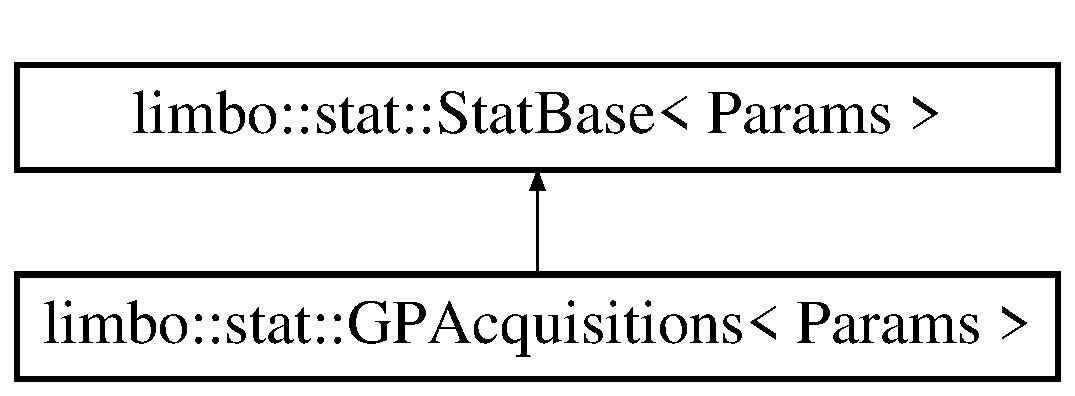
\includegraphics[height=2.000000cm]{structlimbo_1_1stat_1_1_g_p_acquisitions}
\end{center}
\end{figure}
\subsection*{Public Member Functions}
\begin{DoxyCompactItemize}
\item 
{\footnotesize template$<$typename BO , typename Aggregator\+Function $>$ }\\void \hyperlink{structlimbo_1_1stat_1_1_g_p_acquisitions_ac671f5f138d1545bd339068ec5fe4824}{operator()} (const BO \&bo, const Aggregator\+Function \&afun)
\end{DoxyCompactItemize}


\subsection{Detailed Description}
\subsubsection*{template$<$typename Params$>$\\*
struct limbo\+::stat\+::\+G\+P\+Acquisitions$<$ Params $>$}

filename\+: {\ttfamily gp\+\_\+acquisitions.\+dat} 

\subsection{Member Function Documentation}
\index{limbo\+::stat\+::\+G\+P\+Acquisitions@{limbo\+::stat\+::\+G\+P\+Acquisitions}!operator()@{operator()}}
\index{operator()@{operator()}!limbo\+::stat\+::\+G\+P\+Acquisitions@{limbo\+::stat\+::\+G\+P\+Acquisitions}}
\subsubsection[{\texorpdfstring{operator()(const B\+O \&bo, const Aggregator\+Function \&afun)}{operator()(const BO &bo, const AggregatorFunction &afun)}}]{\setlength{\rightskip}{0pt plus 5cm}template$<$typename Params $>$ template$<$typename BO , typename Aggregator\+Function $>$ void {\bf limbo\+::stat\+::\+G\+P\+Acquisitions}$<$ Params $>$\+::operator() (
\begin{DoxyParamCaption}
\item[{const BO \&}]{bo, }
\item[{const Aggregator\+Function \&}]{afun}
\end{DoxyParamCaption}
)\hspace{0.3cm}{\ttfamily [inline]}}\hypertarget{structlimbo_1_1stat_1_1_g_p_acquisitions_ac671f5f138d1545bd339068ec5fe4824}{}\label{structlimbo_1_1stat_1_1_g_p_acquisitions_ac671f5f138d1545bd339068ec5fe4824}


The documentation for this struct was generated from the following file\+:\begin{DoxyCompactItemize}
\item 
/tmp/doc\+\_\+limbo/limbo/src/limbo/stat/\hyperlink{gp__acquisitions_8hpp}{gp\+\_\+acquisitions.\+hpp}\end{DoxyCompactItemize}

\hypertarget{structlimbo_1_1stat_1_1_g_p_kernel_h_params}{}\section{limbo\+:\+:stat\+:\+:G\+P\+Kernel\+H\+Params$<$ Params $>$ Struct Template Reference}
\label{structlimbo_1_1stat_1_1_g_p_kernel_h_params}\index{limbo\+::stat\+::\+G\+P\+Kernel\+H\+Params$<$ Params $>$@{limbo\+::stat\+::\+G\+P\+Kernel\+H\+Params$<$ Params $>$}}


{\ttfamily \#include $<$limbo/stat/gp\+\_\+kernel\+\_\+hparams.\+hpp$>$}

Inheritance diagram for limbo\+:\+:stat\+:\+:G\+P\+Kernel\+H\+Params$<$ Params $>$\+:\begin{figure}[H]
\begin{center}
\leavevmode
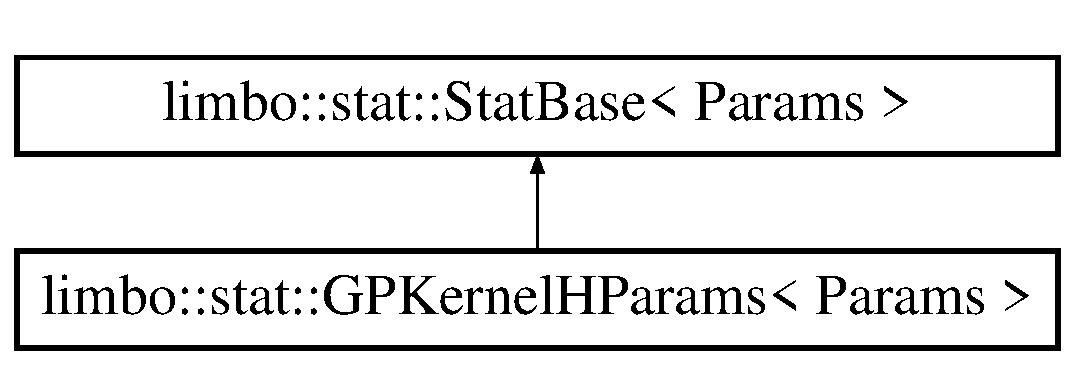
\includegraphics[height=2.000000cm]{structlimbo_1_1stat_1_1_g_p_kernel_h_params}
\end{center}
\end{figure}
\subsection*{Public Member Functions}
\begin{DoxyCompactItemize}
\item 
{\footnotesize template$<$typename B\+O , typename Aggregator\+Function $>$ }\\void \hyperlink{structlimbo_1_1stat_1_1_g_p_kernel_h_params_aa69a6377279cb199ec043ad98b9d5db7}{operator()} (const B\+O \&bo, const Aggregator\+Function \&afun)
\end{DoxyCompactItemize}


\subsection{Detailed Description}
\subsubsection*{template$<$typename Params$>$struct limbo\+::stat\+::\+G\+P\+Kernel\+H\+Params$<$ Params $>$}

filename\+: {\ttfamily gp\+\_\+kernel\+\_\+hparams.\+dat} 

\subsection{Member Function Documentation}
\hypertarget{structlimbo_1_1stat_1_1_g_p_kernel_h_params_aa69a6377279cb199ec043ad98b9d5db7}{}\index{limbo\+::stat\+::\+G\+P\+Kernel\+H\+Params@{limbo\+::stat\+::\+G\+P\+Kernel\+H\+Params}!operator()@{operator()}}
\index{operator()@{operator()}!limbo\+::stat\+::\+G\+P\+Kernel\+H\+Params@{limbo\+::stat\+::\+G\+P\+Kernel\+H\+Params}}
\subsubsection[{operator()}]{\setlength{\rightskip}{0pt plus 5cm}template$<$typename Params $>$ template$<$typename B\+O , typename Aggregator\+Function $>$ void {\bf limbo\+::stat\+::\+G\+P\+Kernel\+H\+Params}$<$ Params $>$\+::operator() (
\begin{DoxyParamCaption}
\item[{const B\+O \&}]{bo, }
\item[{const Aggregator\+Function \&}]{afun}
\end{DoxyParamCaption}
)\hspace{0.3cm}{\ttfamily [inline]}}\label{structlimbo_1_1stat_1_1_g_p_kernel_h_params_aa69a6377279cb199ec043ad98b9d5db7}


The documentation for this struct was generated from the following file\+:\begin{DoxyCompactItemize}
\item 
/tmp/doc\+\_\+limbo/limbo/src/limbo/stat/\hyperlink{gp__kernel__hparams_8hpp}{gp\+\_\+kernel\+\_\+hparams.\+hpp}\end{DoxyCompactItemize}

\hypertarget{structlimbo_1_1stat_1_1_g_p_likelihood}{}\section{limbo\+:\+:stat\+:\+:G\+P\+Likelihood$<$ Params $>$ Struct Template Reference}
\label{structlimbo_1_1stat_1_1_g_p_likelihood}\index{limbo\+::stat\+::\+G\+P\+Likelihood$<$ Params $>$@{limbo\+::stat\+::\+G\+P\+Likelihood$<$ Params $>$}}


{\ttfamily \#include $<$limbo/stat/gp\+\_\+likelihood.\+hpp$>$}

Inheritance diagram for limbo\+:\+:stat\+:\+:G\+P\+Likelihood$<$ Params $>$\+:\begin{figure}[H]
\begin{center}
\leavevmode
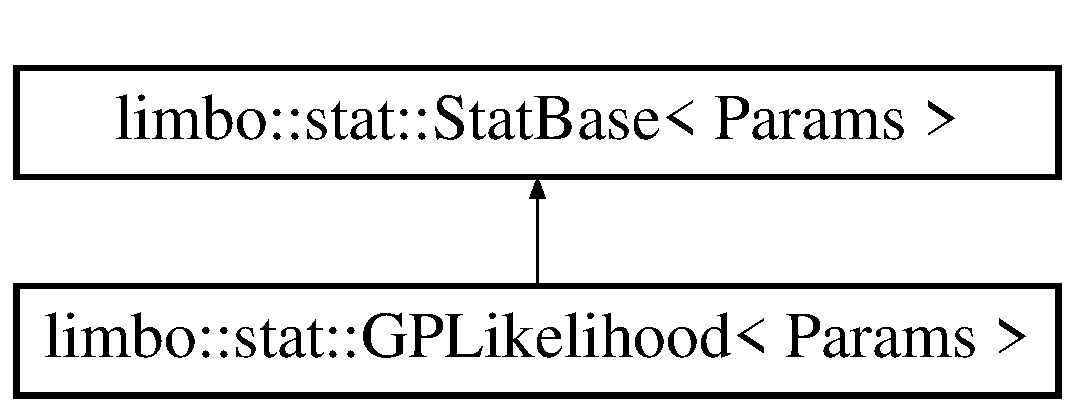
\includegraphics[height=2.000000cm]{structlimbo_1_1stat_1_1_g_p_likelihood}
\end{center}
\end{figure}
\subsection*{Public Member Functions}
\begin{DoxyCompactItemize}
\item 
{\footnotesize template$<$typename B\+O , typename Aggregator\+Function $>$ }\\void \hyperlink{structlimbo_1_1stat_1_1_g_p_likelihood_ac5590ba5e63354d6318d78712c8f6074}{operator()} (const B\+O \&bo, const Aggregator\+Function \&afun)
\end{DoxyCompactItemize}


\subsection{Detailed Description}
\subsubsection*{template$<$typename Params$>$struct limbo\+::stat\+::\+G\+P\+Likelihood$<$ Params $>$}

filename\+: {\ttfamily gp\+\_\+likelihood.\+dat} 

\subsection{Member Function Documentation}
\hypertarget{structlimbo_1_1stat_1_1_g_p_likelihood_ac5590ba5e63354d6318d78712c8f6074}{}\index{limbo\+::stat\+::\+G\+P\+Likelihood@{limbo\+::stat\+::\+G\+P\+Likelihood}!operator()@{operator()}}
\index{operator()@{operator()}!limbo\+::stat\+::\+G\+P\+Likelihood@{limbo\+::stat\+::\+G\+P\+Likelihood}}
\subsubsection[{operator()}]{\setlength{\rightskip}{0pt plus 5cm}template$<$typename Params $>$ template$<$typename B\+O , typename Aggregator\+Function $>$ void {\bf limbo\+::stat\+::\+G\+P\+Likelihood}$<$ Params $>$\+::operator() (
\begin{DoxyParamCaption}
\item[{const B\+O \&}]{bo, }
\item[{const Aggregator\+Function \&}]{afun}
\end{DoxyParamCaption}
)\hspace{0.3cm}{\ttfamily [inline]}}\label{structlimbo_1_1stat_1_1_g_p_likelihood_ac5590ba5e63354d6318d78712c8f6074}


The documentation for this struct was generated from the following file\+:\begin{DoxyCompactItemize}
\item 
/tmp/doc\+\_\+limbo/limbo/src/limbo/stat/\hyperlink{gp__likelihood_8hpp}{gp\+\_\+likelihood.\+hpp}\end{DoxyCompactItemize}

\hypertarget{structlimbo_1_1stat_1_1_g_p_mean_h_params}{}\section{limbo\+:\+:stat\+:\+:G\+P\+Mean\+H\+Params$<$ Params $>$ Struct Template Reference}
\label{structlimbo_1_1stat_1_1_g_p_mean_h_params}\index{limbo\+::stat\+::\+G\+P\+Mean\+H\+Params$<$ Params $>$@{limbo\+::stat\+::\+G\+P\+Mean\+H\+Params$<$ Params $>$}}


{\ttfamily \#include $<$limbo/stat/gp\+\_\+mean\+\_\+hparams.\+hpp$>$}

Inheritance diagram for limbo\+:\+:stat\+:\+:G\+P\+Mean\+H\+Params$<$ Params $>$\+:\begin{figure}[H]
\begin{center}
\leavevmode
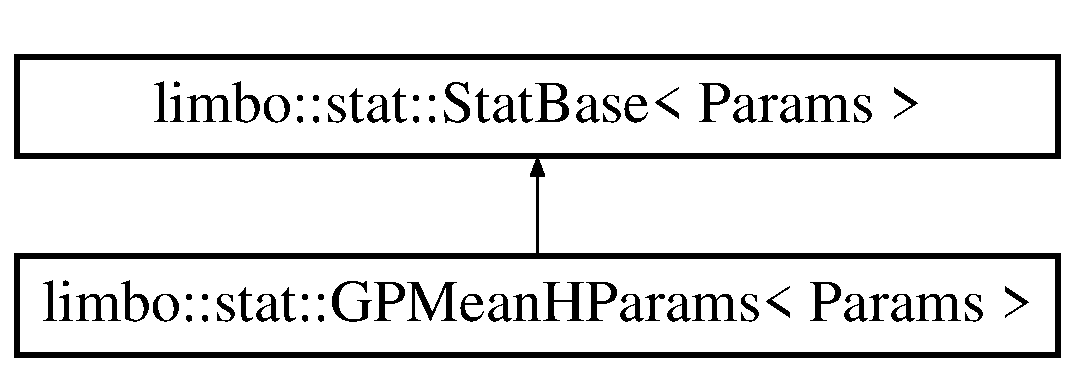
\includegraphics[height=2.000000cm]{structlimbo_1_1stat_1_1_g_p_mean_h_params}
\end{center}
\end{figure}
\subsection*{Public Member Functions}
\begin{DoxyCompactItemize}
\item 
{\footnotesize template$<$typename BO , typename Aggregator\+Function $>$ }\\void \hyperlink{structlimbo_1_1stat_1_1_g_p_mean_h_params_a668c9a82a1ae88273a44f48a4b6f4612}{operator()} (const BO \&bo, const Aggregator\+Function \&afun)
\end{DoxyCompactItemize}


\subsection{Detailed Description}
\subsubsection*{template$<$typename Params$>$\\*
struct limbo\+::stat\+::\+G\+P\+Mean\+H\+Params$<$ Params $>$}

filename\+: {\ttfamily gp\+\_\+mean\+\_\+hparams.\+dat} 

\subsection{Member Function Documentation}
\index{limbo\+::stat\+::\+G\+P\+Mean\+H\+Params@{limbo\+::stat\+::\+G\+P\+Mean\+H\+Params}!operator()@{operator()}}
\index{operator()@{operator()}!limbo\+::stat\+::\+G\+P\+Mean\+H\+Params@{limbo\+::stat\+::\+G\+P\+Mean\+H\+Params}}
\subsubsection[{\texorpdfstring{operator()(const B\+O \&bo, const Aggregator\+Function \&afun)}{operator()(const BO &bo, const AggregatorFunction &afun)}}]{\setlength{\rightskip}{0pt plus 5cm}template$<$typename Params $>$ template$<$typename BO , typename Aggregator\+Function $>$ void {\bf limbo\+::stat\+::\+G\+P\+Mean\+H\+Params}$<$ Params $>$\+::operator() (
\begin{DoxyParamCaption}
\item[{const BO \&}]{bo, }
\item[{const Aggregator\+Function \&}]{afun}
\end{DoxyParamCaption}
)\hspace{0.3cm}{\ttfamily [inline]}}\hypertarget{structlimbo_1_1stat_1_1_g_p_mean_h_params_a668c9a82a1ae88273a44f48a4b6f4612}{}\label{structlimbo_1_1stat_1_1_g_p_mean_h_params_a668c9a82a1ae88273a44f48a4b6f4612}


The documentation for this struct was generated from the following file\+:\begin{DoxyCompactItemize}
\item 
/tmp/doc\+\_\+limbo/limbo/src/limbo/stat/\hyperlink{gp__mean__hparams_8hpp}{gp\+\_\+mean\+\_\+hparams.\+hpp}\end{DoxyCompactItemize}

\hypertarget{classlimbo_1_1experimental_1_1model_1_1_g_p_parego}{}\section{limbo\+:\+:experimental\+:\+:model\+:\+:G\+P\+Parego$<$ Params, Model $>$ Class Template Reference}
\label{classlimbo_1_1experimental_1_1model_1_1_g_p_parego}\index{limbo\+::experimental\+::model\+::\+G\+P\+Parego$<$ Params, Model $>$@{limbo\+::experimental\+::model\+::\+G\+P\+Parego$<$ Params, Model $>$}}


{\ttfamily \#include $<$limbo/experimental/model/gp\+\_\+parego.\+hpp$>$}

Inheritance diagram for limbo\+:\+:experimental\+:\+:model\+:\+:G\+P\+Parego$<$ Params, Model $>$\+:\begin{figure}[H]
\begin{center}
\leavevmode
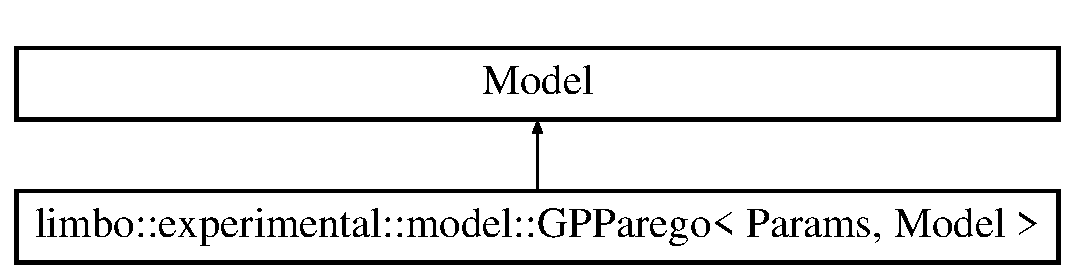
\includegraphics[height=2.000000cm]{classlimbo_1_1experimental_1_1model_1_1_g_p_parego}
\end{center}
\end{figure}
\subsection*{Public Member Functions}
\begin{DoxyCompactItemize}
\item 
\hyperlink{classlimbo_1_1experimental_1_1model_1_1_g_p_parego_ac351d6798add22da5c6dd58ac4a00723}{G\+P\+Parego} ()
\item 
\hyperlink{classlimbo_1_1experimental_1_1model_1_1_g_p_parego_a1f0eb578140f01874b13bfca124c085c}{G\+P\+Parego} (int dim\+\_\+in, int dim\+\_\+out)
\item 
void \hyperlink{classlimbo_1_1experimental_1_1model_1_1_g_p_parego_a81f8ca3a7f114b015575ae7c64183ead}{compute} (const std\+::vector$<$ Eigen\+::\+Vector\+Xd $>$ \&samples, const std\+::vector$<$ Eigen\+::\+Vector\+Xd $>$ \&observations, const Eigen\+::\+Vector\+Xd \&noises, const std\+::vector$<$ Eigen\+::\+Vector\+Xd $>$ \&bl\+\_\+samples=std\+::vector$<$ Eigen\+::\+Vector\+Xd $>$())
\item 
void \hyperlink{classlimbo_1_1experimental_1_1model_1_1_g_p_parego_a81955696f79b4ac11a17d0faf28ccc31}{add\+\_\+sample} (const Eigen\+::\+Vector\+Xd \&sample, const Eigen\+::\+Vector\+Xd \&observation, double noise)
\begin{DoxyCompactList}\small\item\em add sample will N\+O\+T be incremental (we call compute each time) \end{DoxyCompactList}\item 
void \hyperlink{classlimbo_1_1experimental_1_1model_1_1_g_p_parego_aee0ce034411e11614069718a3140a3f8}{add\+\_\+bl\+\_\+sample} (const Eigen\+::\+Vector\+Xd \&bl\+\_\+sample, double noise)
\begin{DoxyCompactList}\small\item\em W\+A\+R\+N\+I\+N\+G\+: Parego does not really work with blacklisted samples. \end{DoxyCompactList}\end{DoxyCompactItemize}


\subsection{Detailed Description}
\subsubsection*{template$<$typename Params, typename Model$>$class limbo\+::experimental\+::model\+::\+G\+P\+Parego$<$ Params, Model $>$}

this is the model used in Parego reference\+: Knowles, J. (2006). Par\+E\+G\+O\+: A hybrid algorithm with on-\/line landscape approximation for expensive multiobjective optimization problems. I\+E\+E\+E Transactions On Evolutionary Computation, 10(1), 50-\/66. Main idea\+:
\begin{DoxyItemize}
\item this models aggregates all the objective values with the Tchebycheff distance
\item objectives are weighted using a random vector
\item a single model is built 
\end{DoxyItemize}

\subsection{Constructor \& Destructor Documentation}
\hypertarget{classlimbo_1_1experimental_1_1model_1_1_g_p_parego_ac351d6798add22da5c6dd58ac4a00723}{}\index{limbo\+::experimental\+::model\+::\+G\+P\+Parego@{limbo\+::experimental\+::model\+::\+G\+P\+Parego}!G\+P\+Parego@{G\+P\+Parego}}
\index{G\+P\+Parego@{G\+P\+Parego}!limbo\+::experimental\+::model\+::\+G\+P\+Parego@{limbo\+::experimental\+::model\+::\+G\+P\+Parego}}
\subsubsection[{G\+P\+Parego}]{\setlength{\rightskip}{0pt plus 5cm}template$<$typename Params , typename Model $>$ {\bf limbo\+::experimental\+::model\+::\+G\+P\+Parego}$<$ Params, Model $>$\+::{\bf G\+P\+Parego} (
\begin{DoxyParamCaption}
{}
\end{DoxyParamCaption}
)\hspace{0.3cm}{\ttfamily [inline]}}\label{classlimbo_1_1experimental_1_1model_1_1_g_p_parego_ac351d6798add22da5c6dd58ac4a00723}
\hypertarget{classlimbo_1_1experimental_1_1model_1_1_g_p_parego_a1f0eb578140f01874b13bfca124c085c}{}\index{limbo\+::experimental\+::model\+::\+G\+P\+Parego@{limbo\+::experimental\+::model\+::\+G\+P\+Parego}!G\+P\+Parego@{G\+P\+Parego}}
\index{G\+P\+Parego@{G\+P\+Parego}!limbo\+::experimental\+::model\+::\+G\+P\+Parego@{limbo\+::experimental\+::model\+::\+G\+P\+Parego}}
\subsubsection[{G\+P\+Parego}]{\setlength{\rightskip}{0pt plus 5cm}template$<$typename Params , typename Model $>$ {\bf limbo\+::experimental\+::model\+::\+G\+P\+Parego}$<$ Params, Model $>$\+::{\bf G\+P\+Parego} (
\begin{DoxyParamCaption}
\item[{int}]{dim\+\_\+in, }
\item[{int}]{dim\+\_\+out}
\end{DoxyParamCaption}
)\hspace{0.3cm}{\ttfamily [inline]}}\label{classlimbo_1_1experimental_1_1model_1_1_g_p_parego_a1f0eb578140f01874b13bfca124c085c}


\subsection{Member Function Documentation}
\hypertarget{classlimbo_1_1experimental_1_1model_1_1_g_p_parego_aee0ce034411e11614069718a3140a3f8}{}\index{limbo\+::experimental\+::model\+::\+G\+P\+Parego@{limbo\+::experimental\+::model\+::\+G\+P\+Parego}!add\+\_\+bl\+\_\+sample@{add\+\_\+bl\+\_\+sample}}
\index{add\+\_\+bl\+\_\+sample@{add\+\_\+bl\+\_\+sample}!limbo\+::experimental\+::model\+::\+G\+P\+Parego@{limbo\+::experimental\+::model\+::\+G\+P\+Parego}}
\subsubsection[{add\+\_\+bl\+\_\+sample}]{\setlength{\rightskip}{0pt plus 5cm}template$<$typename Params , typename Model $>$ void {\bf limbo\+::experimental\+::model\+::\+G\+P\+Parego}$<$ Params, Model $>$\+::add\+\_\+bl\+\_\+sample (
\begin{DoxyParamCaption}
\item[{const Eigen\+::\+Vector\+Xd \&}]{bl\+\_\+sample, }
\item[{double}]{noise}
\end{DoxyParamCaption}
)\hspace{0.3cm}{\ttfamily [inline]}}\label{classlimbo_1_1experimental_1_1model_1_1_g_p_parego_aee0ce034411e11614069718a3140a3f8}


W\+A\+R\+N\+I\+N\+G\+: Parego does not really work with blacklisted samples. 

\hypertarget{classlimbo_1_1experimental_1_1model_1_1_g_p_parego_a81955696f79b4ac11a17d0faf28ccc31}{}\index{limbo\+::experimental\+::model\+::\+G\+P\+Parego@{limbo\+::experimental\+::model\+::\+G\+P\+Parego}!add\+\_\+sample@{add\+\_\+sample}}
\index{add\+\_\+sample@{add\+\_\+sample}!limbo\+::experimental\+::model\+::\+G\+P\+Parego@{limbo\+::experimental\+::model\+::\+G\+P\+Parego}}
\subsubsection[{add\+\_\+sample}]{\setlength{\rightskip}{0pt plus 5cm}template$<$typename Params , typename Model $>$ void {\bf limbo\+::experimental\+::model\+::\+G\+P\+Parego}$<$ Params, Model $>$\+::add\+\_\+sample (
\begin{DoxyParamCaption}
\item[{const Eigen\+::\+Vector\+Xd \&}]{sample, }
\item[{const Eigen\+::\+Vector\+Xd \&}]{observation, }
\item[{double}]{noise}
\end{DoxyParamCaption}
)\hspace{0.3cm}{\ttfamily [inline]}}\label{classlimbo_1_1experimental_1_1model_1_1_g_p_parego_a81955696f79b4ac11a17d0faf28ccc31}


add sample will N\+O\+T be incremental (we call compute each time) 

\hypertarget{classlimbo_1_1experimental_1_1model_1_1_g_p_parego_a81f8ca3a7f114b015575ae7c64183ead}{}\index{limbo\+::experimental\+::model\+::\+G\+P\+Parego@{limbo\+::experimental\+::model\+::\+G\+P\+Parego}!compute@{compute}}
\index{compute@{compute}!limbo\+::experimental\+::model\+::\+G\+P\+Parego@{limbo\+::experimental\+::model\+::\+G\+P\+Parego}}
\subsubsection[{compute}]{\setlength{\rightskip}{0pt plus 5cm}template$<$typename Params , typename Model $>$ void {\bf limbo\+::experimental\+::model\+::\+G\+P\+Parego}$<$ Params, Model $>$\+::compute (
\begin{DoxyParamCaption}
\item[{const std\+::vector$<$ Eigen\+::\+Vector\+Xd $>$ \&}]{samples, }
\item[{const std\+::vector$<$ Eigen\+::\+Vector\+Xd $>$ \&}]{observations, }
\item[{const Eigen\+::\+Vector\+Xd \&}]{noises, }
\item[{const std\+::vector$<$ Eigen\+::\+Vector\+Xd $>$ \&}]{bl\+\_\+samples = {\ttfamily std\+:\+:vector$<$Eigen\+:\+:VectorXd$>$()}}
\end{DoxyParamCaption}
)\hspace{0.3cm}{\ttfamily [inline]}}\label{classlimbo_1_1experimental_1_1model_1_1_g_p_parego_a81f8ca3a7f114b015575ae7c64183ead}


The documentation for this class was generated from the following file\+:\begin{DoxyCompactItemize}
\item 
/tmp/doc\+\_\+limbo/limbo/src/limbo/experimental/model/\hyperlink{gp__parego_8hpp}{gp\+\_\+parego.\+hpp}\end{DoxyCompactItemize}

\hypertarget{structlimbo_1_1stat_1_1_g_p_prediction_differences}{}\section{limbo\+:\+:stat\+:\+:G\+P\+Prediction\+Differences$<$ Params $>$ Struct Template Reference}
\label{structlimbo_1_1stat_1_1_g_p_prediction_differences}\index{limbo\+::stat\+::\+G\+P\+Prediction\+Differences$<$ Params $>$@{limbo\+::stat\+::\+G\+P\+Prediction\+Differences$<$ Params $>$}}


{\ttfamily \#include $<$limbo/stat/gp\+\_\+prediction\+\_\+differences.\+hpp$>$}

Inheritance diagram for limbo\+:\+:stat\+:\+:G\+P\+Prediction\+Differences$<$ Params $>$\+:\begin{figure}[H]
\begin{center}
\leavevmode
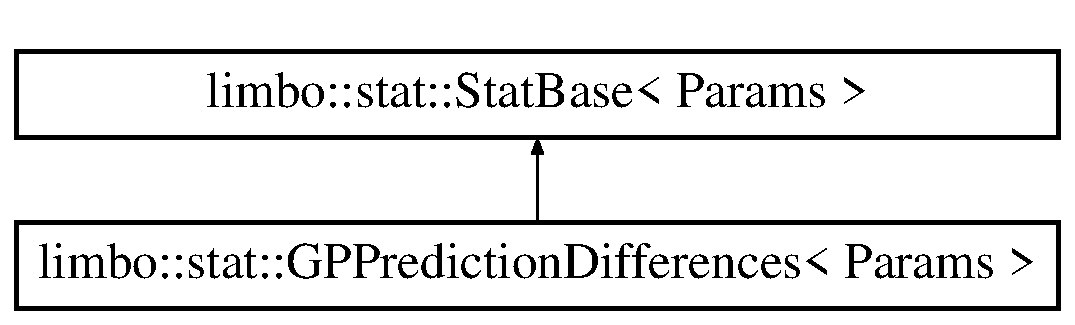
\includegraphics[height=2.000000cm]{structlimbo_1_1stat_1_1_g_p_prediction_differences}
\end{center}
\end{figure}
\subsection*{Public Member Functions}
\begin{DoxyCompactItemize}
\item 
{\footnotesize template$<$typename BO , typename Aggregator\+Function $>$ }\\void \hyperlink{structlimbo_1_1stat_1_1_g_p_prediction_differences_a91a2d59457d83adbbfa6138db9e200cd}{operator()} (const BO \&bo, const Aggregator\+Function \&afun)
\end{DoxyCompactItemize}


\subsection{Detailed Description}
\subsubsection*{template$<$typename Params$>$\\*
struct limbo\+::stat\+::\+G\+P\+Prediction\+Differences$<$ Params $>$}

filename\+: {\ttfamily gp\+\_\+prediction\+\_\+differences.\+dat} 

\subsection{Member Function Documentation}
\index{limbo\+::stat\+::\+G\+P\+Prediction\+Differences@{limbo\+::stat\+::\+G\+P\+Prediction\+Differences}!operator()@{operator()}}
\index{operator()@{operator()}!limbo\+::stat\+::\+G\+P\+Prediction\+Differences@{limbo\+::stat\+::\+G\+P\+Prediction\+Differences}}
\subsubsection[{\texorpdfstring{operator()(const B\+O \&bo, const Aggregator\+Function \&afun)}{operator()(const BO &bo, const AggregatorFunction &afun)}}]{\setlength{\rightskip}{0pt plus 5cm}template$<$typename Params $>$ template$<$typename BO , typename Aggregator\+Function $>$ void {\bf limbo\+::stat\+::\+G\+P\+Prediction\+Differences}$<$ Params $>$\+::operator() (
\begin{DoxyParamCaption}
\item[{const BO \&}]{bo, }
\item[{const Aggregator\+Function \&}]{afun}
\end{DoxyParamCaption}
)\hspace{0.3cm}{\ttfamily [inline]}}\hypertarget{structlimbo_1_1stat_1_1_g_p_prediction_differences_a91a2d59457d83adbbfa6138db9e200cd}{}\label{structlimbo_1_1stat_1_1_g_p_prediction_differences_a91a2d59457d83adbbfa6138db9e200cd}


The documentation for this struct was generated from the following file\+:\begin{DoxyCompactItemize}
\item 
/tmp/doc\+\_\+limbo/limbo/src/limbo/stat/\hyperlink{gp__prediction__differences_8hpp}{gp\+\_\+prediction\+\_\+differences.\+hpp}\end{DoxyCompactItemize}

\hypertarget{structlimbo_1_1init_1_1_grid_sampling}{}\section{limbo\+:\+:init\+:\+:Grid\+Sampling$<$ Params $>$ Struct Template Reference}
\label{structlimbo_1_1init_1_1_grid_sampling}\index{limbo\+::init\+::\+Grid\+Sampling$<$ Params $>$@{limbo\+::init\+::\+Grid\+Sampling$<$ Params $>$}}


{\ttfamily \#include $<$limbo/init/grid\+\_\+sampling.\+hpp$>$}

\subsection*{Public Member Functions}
\begin{DoxyCompactItemize}
\item 
{\footnotesize template$<$typename State\+Function , typename Aggregator\+Function , typename Opt $>$ }\\void \hyperlink{structlimbo_1_1init_1_1_grid_sampling_a9b17fba72e1ae09a3361e9dcb8ff3fe3}{operator()} (const State\+Function \&seval, const Aggregator\+Function \&, Opt \&opt) const 
\end{DoxyCompactItemize}


\subsection{Detailed Description}
\subsubsection*{template$<$typename Params$>$\\*
struct limbo\+::init\+::\+Grid\+Sampling$<$ Params $>$}

\begin{DoxyVerb}embed:rst
Grid sampling.

Parameter:
  - ``int bins`` (number of bins)
\end{DoxyVerb}
 

\subsection{Member Function Documentation}
\index{limbo\+::init\+::\+Grid\+Sampling@{limbo\+::init\+::\+Grid\+Sampling}!operator()@{operator()}}
\index{operator()@{operator()}!limbo\+::init\+::\+Grid\+Sampling@{limbo\+::init\+::\+Grid\+Sampling}}
\subsubsection[{\texorpdfstring{operator()(const State\+Function \&seval, const Aggregator\+Function \&, Opt \&opt) const }{operator()(const StateFunction &seval, const AggregatorFunction &, Opt &opt) const }}]{\setlength{\rightskip}{0pt plus 5cm}template$<$typename Params $>$ template$<$typename State\+Function , typename Aggregator\+Function , typename Opt $>$ void {\bf limbo\+::init\+::\+Grid\+Sampling}$<$ Params $>$\+::operator() (
\begin{DoxyParamCaption}
\item[{const State\+Function \&}]{seval, }
\item[{const Aggregator\+Function \&}]{, }
\item[{Opt \&}]{opt}
\end{DoxyParamCaption}
) const\hspace{0.3cm}{\ttfamily [inline]}}\hypertarget{structlimbo_1_1init_1_1_grid_sampling_a9b17fba72e1ae09a3361e9dcb8ff3fe3}{}\label{structlimbo_1_1init_1_1_grid_sampling_a9b17fba72e1ae09a3361e9dcb8ff3fe3}


The documentation for this struct was generated from the following file\+:\begin{DoxyCompactItemize}
\item 
/tmp/doc\+\_\+limbo/limbo/src/limbo/init/\hyperlink{grid__sampling_8hpp}{grid\+\_\+sampling.\+hpp}\end{DoxyCompactItemize}

\hypertarget{structlimbo_1_1opt_1_1_grid_search}{}\section{limbo\+:\+:opt\+:\+:Grid\+Search$<$ Params $>$ Struct Template Reference}
\label{structlimbo_1_1opt_1_1_grid_search}\index{limbo\+::opt\+::\+Grid\+Search$<$ Params $>$@{limbo\+::opt\+::\+Grid\+Search$<$ Params $>$}}


{\ttfamily \#include $<$limbo/opt/grid\+\_\+search.\+hpp$>$}

\subsection*{Public Member Functions}
\begin{DoxyCompactItemize}
\item 
{\footnotesize template$<$typename F $>$ }\\Eigen\+::\+Vector\+Xd \hyperlink{structlimbo_1_1opt_1_1_grid_search_a33545a99e631d9e35776a7d7a582c8a2}{operator()} (const F \&f, const Eigen\+::\+Vector\+Xd \&init, bool bounded) const 
\end{DoxyCompactItemize}


\subsection{Detailed Description}
\subsubsection*{template$<$typename Params$>$\\*
struct limbo\+::opt\+::\+Grid\+Search$<$ Params $>$}

Grid search

Parameters\+:
\begin{DoxyItemize}
\item int bins 
\end{DoxyItemize}

\subsection{Member Function Documentation}
\index{limbo\+::opt\+::\+Grid\+Search@{limbo\+::opt\+::\+Grid\+Search}!operator()@{operator()}}
\index{operator()@{operator()}!limbo\+::opt\+::\+Grid\+Search@{limbo\+::opt\+::\+Grid\+Search}}
\subsubsection[{\texorpdfstring{operator()(const F \&f, const Eigen\+::\+Vector\+Xd \&init, bool bounded) const }{operator()(const F &f, const Eigen::VectorXd &init, bool bounded) const }}]{\setlength{\rightskip}{0pt plus 5cm}template$<$typename Params $>$ template$<$typename F $>$ Eigen\+::\+Vector\+Xd {\bf limbo\+::opt\+::\+Grid\+Search}$<$ Params $>$\+::operator() (
\begin{DoxyParamCaption}
\item[{const F \&}]{f, }
\item[{const Eigen\+::\+Vector\+Xd \&}]{init, }
\item[{bool}]{bounded}
\end{DoxyParamCaption}
) const\hspace{0.3cm}{\ttfamily [inline]}}\hypertarget{structlimbo_1_1opt_1_1_grid_search_a33545a99e631d9e35776a7d7a582c8a2}{}\label{structlimbo_1_1opt_1_1_grid_search_a33545a99e631d9e35776a7d7a582c8a2}


The documentation for this struct was generated from the following file\+:\begin{DoxyCompactItemize}
\item 
/tmp/doc\+\_\+limbo/limbo/src/limbo/opt/\hyperlink{grid__search_8hpp}{grid\+\_\+search.\+hpp}\end{DoxyCompactItemize}

\hypertarget{structlimbo_1_1experimental_1_1stat_1_1_hyper_volume}{}\section{limbo\+:\+:experimental\+:\+:stat\+:\+:Hyper\+Volume$<$ Params $>$ Struct Template Reference}
\label{structlimbo_1_1experimental_1_1stat_1_1_hyper_volume}\index{limbo\+::experimental\+::stat\+::\+Hyper\+Volume$<$ Params $>$@{limbo\+::experimental\+::stat\+::\+Hyper\+Volume$<$ Params $>$}}


{\ttfamily \#include $<$limbo/experimental/stat/hyper\+\_\+volume.\+hpp$>$}

Inheritance diagram for limbo\+:\+:experimental\+:\+:stat\+:\+:Hyper\+Volume$<$ Params $>$\+:\begin{figure}[H]
\begin{center}
\leavevmode
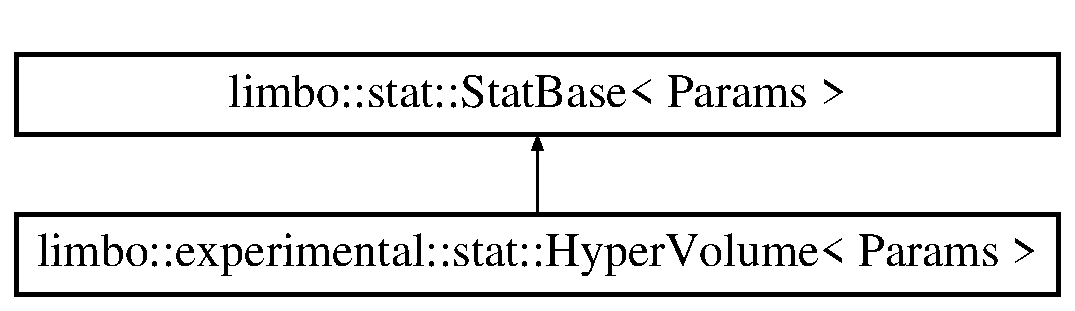
\includegraphics[height=2.000000cm]{structlimbo_1_1experimental_1_1stat_1_1_hyper_volume}
\end{center}
\end{figure}
\subsection*{Public Member Functions}
\begin{DoxyCompactItemize}
\item 
{\footnotesize template$<$typename BO , typename Aggregator\+Function $>$ }\\void \hyperlink{structlimbo_1_1experimental_1_1stat_1_1_hyper_volume_a1ed1a3d3a92f8cdc115a34bb984466ce}{operator()} (const BO \&bo, const Aggregator\+Function \&)
\end{DoxyCompactItemize}


\subsection{Member Function Documentation}
\index{limbo\+::experimental\+::stat\+::\+Hyper\+Volume@{limbo\+::experimental\+::stat\+::\+Hyper\+Volume}!operator()@{operator()}}
\index{operator()@{operator()}!limbo\+::experimental\+::stat\+::\+Hyper\+Volume@{limbo\+::experimental\+::stat\+::\+Hyper\+Volume}}
\subsubsection[{\texorpdfstring{operator()(const B\+O \&bo, const Aggregator\+Function \&)}{operator()(const BO &bo, const AggregatorFunction &)}}]{\setlength{\rightskip}{0pt plus 5cm}template$<$typename Params $>$ template$<$typename BO , typename Aggregator\+Function $>$ void {\bf limbo\+::experimental\+::stat\+::\+Hyper\+Volume}$<$ Params $>$\+::operator() (
\begin{DoxyParamCaption}
\item[{const BO \&}]{bo, }
\item[{const Aggregator\+Function \&}]{}
\end{DoxyParamCaption}
)\hspace{0.3cm}{\ttfamily [inline]}}\hypertarget{structlimbo_1_1experimental_1_1stat_1_1_hyper_volume_a1ed1a3d3a92f8cdc115a34bb984466ce}{}\label{structlimbo_1_1experimental_1_1stat_1_1_hyper_volume_a1ed1a3d3a92f8cdc115a34bb984466ce}


The documentation for this struct was generated from the following file\+:\begin{DoxyCompactItemize}
\item 
/tmp/doc\+\_\+limbo/limbo/src/limbo/experimental/stat/\hyperlink{hyper__volume_8hpp}{hyper\+\_\+volume.\+hpp}\end{DoxyCompactItemize}

\hypertarget{classlimbo_1_1bayes__opt_1_1experimental_1_1_i_m_g_p_o}{}\section{limbo\+:\+:bayes\+\_\+opt\+:\+:experimental\+:\+:I\+M\+G\+P\+O$<$ Params, A1, A2, A3, A4, A5 $>$ Class Template Reference}
\label{classlimbo_1_1bayes__opt_1_1experimental_1_1_i_m_g_p_o}\index{limbo\+::bayes\+\_\+opt\+::experimental\+::\+I\+M\+G\+P\+O$<$ Params, A1, A2, A3, A4, A5 $>$@{limbo\+::bayes\+\_\+opt\+::experimental\+::\+I\+M\+G\+P\+O$<$ Params, A1, A2, A3, A4, A5 $>$}}


{\ttfamily \#include $<$limbo/experimental/bayes\+\_\+opt/imgpo.\+hpp$>$}

Inheritance diagram for limbo\+:\+:bayes\+\_\+opt\+:\+:experimental\+:\+:I\+M\+G\+P\+O$<$ Params, A1, A2, A3, A4, A5 $>$\+:\begin{figure}[H]
\begin{center}
\leavevmode
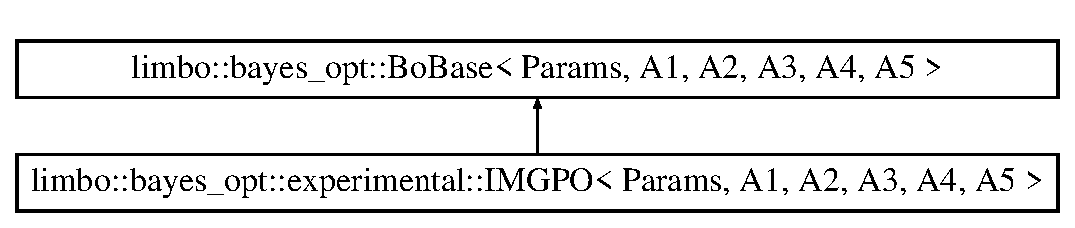
\includegraphics[height=2.000000cm]{classlimbo_1_1bayes__opt_1_1experimental_1_1_i_m_g_p_o}
\end{center}
\end{figure}
\subsection*{Public Types}
\begin{DoxyCompactItemize}
\item 
typedef \hyperlink{classlimbo_1_1bayes__opt_1_1_bo_base}{Bo\+Base}$<$ Params, A1, A2, A3, A4, A5 $>$ \hyperlink{classlimbo_1_1bayes__opt_1_1experimental_1_1_i_m_g_p_o_a08e12049587eed6be7bc86f05da043f0}{base\+\_\+t}
\item 
typedef \hyperlink{classlimbo_1_1bayes__opt_1_1_bo_base_a1ddc93cc023a2d7d527deb4cc750624e}{base\+\_\+t\+::model\+\_\+t} \hyperlink{classlimbo_1_1bayes__opt_1_1experimental_1_1_i_m_g_p_o_a2a2958dccaec1f7f1b21a2d4c85cf1fc}{model\+\_\+t}
\item 
typedef \hyperlink{classlimbo_1_1bayes__opt_1_1_bo_base_a02b14991b62e0f8c9bcf834220ed62e4}{base\+\_\+t\+::acquisition\+\_\+function\+\_\+t} \hyperlink{classlimbo_1_1bayes__opt_1_1experimental_1_1_i_m_g_p_o_af7f26bfe0e3119ce147088e9e8fbfc17}{acquisition\+\_\+function\+\_\+t}
\end{DoxyCompactItemize}
\subsection*{Public Member Functions}
\begin{DoxyCompactItemize}
\item 
{\footnotesize template$<$typename State\+Function , typename Aggregator\+Function  = First\+Elem$>$ }\\void \hyperlink{classlimbo_1_1bayes__opt_1_1experimental_1_1_i_m_g_p_o_afbee4ff7950e1f0f2f98962211fb4ae4}{optimize} (const State\+Function \&sfun, const Aggregator\+Function \&afun=Aggregator\+Function(), bool reset=true)
\item 
{\footnotesize template$<$typename Aggregator\+Function  = First\+Elem$>$ }\\const Eigen\+::\+Vector\+Xd \& \hyperlink{classlimbo_1_1bayes__opt_1_1experimental_1_1_i_m_g_p_o_a1724761e5705e64b01acfff23c0b2c28}{best\+\_\+observation} (const Aggregator\+Function \&afun=Aggregator\+Function()) const 
\item 
{\footnotesize template$<$typename Aggregator\+Function  = First\+Elem$>$ }\\const Eigen\+::\+Vector\+Xd \& \hyperlink{classlimbo_1_1bayes__opt_1_1experimental_1_1_i_m_g_p_o_aeafb58cec2621c70ea4db4806272dc0b}{best\+\_\+sample} (const Aggregator\+Function \&afun=Aggregator\+Function()) const 
\item 
const \hyperlink{classlimbo_1_1bayes__opt_1_1_bo_base_a1ddc93cc023a2d7d527deb4cc750624e}{model\+\_\+t} \& \hyperlink{classlimbo_1_1bayes__opt_1_1experimental_1_1_i_m_g_p_o_ac0ee4f560d2629dd6a738a79d669f580}{model} () const 
\end{DoxyCompactItemize}


\subsection{Member Typedef Documentation}
\hypertarget{classlimbo_1_1bayes__opt_1_1experimental_1_1_i_m_g_p_o_af7f26bfe0e3119ce147088e9e8fbfc17}{}\index{limbo\+::bayes\+\_\+opt\+::experimental\+::\+I\+M\+G\+P\+O@{limbo\+::bayes\+\_\+opt\+::experimental\+::\+I\+M\+G\+P\+O}!acquisition\+\_\+function\+\_\+t@{acquisition\+\_\+function\+\_\+t}}
\index{acquisition\+\_\+function\+\_\+t@{acquisition\+\_\+function\+\_\+t}!limbo\+::bayes\+\_\+opt\+::experimental\+::\+I\+M\+G\+P\+O@{limbo\+::bayes\+\_\+opt\+::experimental\+::\+I\+M\+G\+P\+O}}
\subsubsection[{acquisition\+\_\+function\+\_\+t}]{\setlength{\rightskip}{0pt plus 5cm}template$<$class Params , class A1  = boost\+::parameter\+::void\+\_\+, class A2  = boost\+::parameter\+::void\+\_\+, class A3  = boost\+::parameter\+::void\+\_\+, class A4  = boost\+::parameter\+::void\+\_\+, class A5  = boost\+::parameter\+::void\+\_\+$>$ typedef {\bf base\+\_\+t\+::acquisition\+\_\+function\+\_\+t} {\bf limbo\+::bayes\+\_\+opt\+::experimental\+::\+I\+M\+G\+P\+O}$<$ Params, A1, A2, A3, A4, A5 $>$\+::{\bf acquisition\+\_\+function\+\_\+t}}\label{classlimbo_1_1bayes__opt_1_1experimental_1_1_i_m_g_p_o_af7f26bfe0e3119ce147088e9e8fbfc17}
\hypertarget{classlimbo_1_1bayes__opt_1_1experimental_1_1_i_m_g_p_o_a08e12049587eed6be7bc86f05da043f0}{}\index{limbo\+::bayes\+\_\+opt\+::experimental\+::\+I\+M\+G\+P\+O@{limbo\+::bayes\+\_\+opt\+::experimental\+::\+I\+M\+G\+P\+O}!base\+\_\+t@{base\+\_\+t}}
\index{base\+\_\+t@{base\+\_\+t}!limbo\+::bayes\+\_\+opt\+::experimental\+::\+I\+M\+G\+P\+O@{limbo\+::bayes\+\_\+opt\+::experimental\+::\+I\+M\+G\+P\+O}}
\subsubsection[{base\+\_\+t}]{\setlength{\rightskip}{0pt plus 5cm}template$<$class Params , class A1  = boost\+::parameter\+::void\+\_\+, class A2  = boost\+::parameter\+::void\+\_\+, class A3  = boost\+::parameter\+::void\+\_\+, class A4  = boost\+::parameter\+::void\+\_\+, class A5  = boost\+::parameter\+::void\+\_\+$>$ typedef {\bf Bo\+Base}$<$Params, A1, A2, A3, A4, A5$>$ {\bf limbo\+::bayes\+\_\+opt\+::experimental\+::\+I\+M\+G\+P\+O}$<$ Params, A1, A2, A3, A4, A5 $>$\+::{\bf base\+\_\+t}}\label{classlimbo_1_1bayes__opt_1_1experimental_1_1_i_m_g_p_o_a08e12049587eed6be7bc86f05da043f0}
\hypertarget{classlimbo_1_1bayes__opt_1_1experimental_1_1_i_m_g_p_o_a2a2958dccaec1f7f1b21a2d4c85cf1fc}{}\index{limbo\+::bayes\+\_\+opt\+::experimental\+::\+I\+M\+G\+P\+O@{limbo\+::bayes\+\_\+opt\+::experimental\+::\+I\+M\+G\+P\+O}!model\+\_\+t@{model\+\_\+t}}
\index{model\+\_\+t@{model\+\_\+t}!limbo\+::bayes\+\_\+opt\+::experimental\+::\+I\+M\+G\+P\+O@{limbo\+::bayes\+\_\+opt\+::experimental\+::\+I\+M\+G\+P\+O}}
\subsubsection[{model\+\_\+t}]{\setlength{\rightskip}{0pt plus 5cm}template$<$class Params , class A1  = boost\+::parameter\+::void\+\_\+, class A2  = boost\+::parameter\+::void\+\_\+, class A3  = boost\+::parameter\+::void\+\_\+, class A4  = boost\+::parameter\+::void\+\_\+, class A5  = boost\+::parameter\+::void\+\_\+$>$ typedef {\bf base\+\_\+t\+::model\+\_\+t} {\bf limbo\+::bayes\+\_\+opt\+::experimental\+::\+I\+M\+G\+P\+O}$<$ Params, A1, A2, A3, A4, A5 $>$\+::{\bf model\+\_\+t}}\label{classlimbo_1_1bayes__opt_1_1experimental_1_1_i_m_g_p_o_a2a2958dccaec1f7f1b21a2d4c85cf1fc}


\subsection{Member Function Documentation}
\hypertarget{classlimbo_1_1bayes__opt_1_1experimental_1_1_i_m_g_p_o_a1724761e5705e64b01acfff23c0b2c28}{}\index{limbo\+::bayes\+\_\+opt\+::experimental\+::\+I\+M\+G\+P\+O@{limbo\+::bayes\+\_\+opt\+::experimental\+::\+I\+M\+G\+P\+O}!best\+\_\+observation@{best\+\_\+observation}}
\index{best\+\_\+observation@{best\+\_\+observation}!limbo\+::bayes\+\_\+opt\+::experimental\+::\+I\+M\+G\+P\+O@{limbo\+::bayes\+\_\+opt\+::experimental\+::\+I\+M\+G\+P\+O}}
\subsubsection[{best\+\_\+observation}]{\setlength{\rightskip}{0pt plus 5cm}template$<$class Params , class A1  = boost\+::parameter\+::void\+\_\+, class A2  = boost\+::parameter\+::void\+\_\+, class A3  = boost\+::parameter\+::void\+\_\+, class A4  = boost\+::parameter\+::void\+\_\+, class A5  = boost\+::parameter\+::void\+\_\+$>$ template$<$typename Aggregator\+Function  = First\+Elem$>$ const Eigen\+::\+Vector\+Xd\& {\bf limbo\+::bayes\+\_\+opt\+::experimental\+::\+I\+M\+G\+P\+O}$<$ Params, A1, A2, A3, A4, A5 $>$\+::best\+\_\+observation (
\begin{DoxyParamCaption}
\item[{const Aggregator\+Function \&}]{afun = {\ttfamily AggregatorFunction()}}
\end{DoxyParamCaption}
) const\hspace{0.3cm}{\ttfamily [inline]}}\label{classlimbo_1_1bayes__opt_1_1experimental_1_1_i_m_g_p_o_a1724761e5705e64b01acfff23c0b2c28}
\hypertarget{classlimbo_1_1bayes__opt_1_1experimental_1_1_i_m_g_p_o_aeafb58cec2621c70ea4db4806272dc0b}{}\index{limbo\+::bayes\+\_\+opt\+::experimental\+::\+I\+M\+G\+P\+O@{limbo\+::bayes\+\_\+opt\+::experimental\+::\+I\+M\+G\+P\+O}!best\+\_\+sample@{best\+\_\+sample}}
\index{best\+\_\+sample@{best\+\_\+sample}!limbo\+::bayes\+\_\+opt\+::experimental\+::\+I\+M\+G\+P\+O@{limbo\+::bayes\+\_\+opt\+::experimental\+::\+I\+M\+G\+P\+O}}
\subsubsection[{best\+\_\+sample}]{\setlength{\rightskip}{0pt plus 5cm}template$<$class Params , class A1  = boost\+::parameter\+::void\+\_\+, class A2  = boost\+::parameter\+::void\+\_\+, class A3  = boost\+::parameter\+::void\+\_\+, class A4  = boost\+::parameter\+::void\+\_\+, class A5  = boost\+::parameter\+::void\+\_\+$>$ template$<$typename Aggregator\+Function  = First\+Elem$>$ const Eigen\+::\+Vector\+Xd\& {\bf limbo\+::bayes\+\_\+opt\+::experimental\+::\+I\+M\+G\+P\+O}$<$ Params, A1, A2, A3, A4, A5 $>$\+::best\+\_\+sample (
\begin{DoxyParamCaption}
\item[{const Aggregator\+Function \&}]{afun = {\ttfamily AggregatorFunction()}}
\end{DoxyParamCaption}
) const\hspace{0.3cm}{\ttfamily [inline]}}\label{classlimbo_1_1bayes__opt_1_1experimental_1_1_i_m_g_p_o_aeafb58cec2621c70ea4db4806272dc0b}
\hypertarget{classlimbo_1_1bayes__opt_1_1experimental_1_1_i_m_g_p_o_ac0ee4f560d2629dd6a738a79d669f580}{}\index{limbo\+::bayes\+\_\+opt\+::experimental\+::\+I\+M\+G\+P\+O@{limbo\+::bayes\+\_\+opt\+::experimental\+::\+I\+M\+G\+P\+O}!model@{model}}
\index{model@{model}!limbo\+::bayes\+\_\+opt\+::experimental\+::\+I\+M\+G\+P\+O@{limbo\+::bayes\+\_\+opt\+::experimental\+::\+I\+M\+G\+P\+O}}
\subsubsection[{model}]{\setlength{\rightskip}{0pt plus 5cm}template$<$class Params , class A1  = boost\+::parameter\+::void\+\_\+, class A2  = boost\+::parameter\+::void\+\_\+, class A3  = boost\+::parameter\+::void\+\_\+, class A4  = boost\+::parameter\+::void\+\_\+, class A5  = boost\+::parameter\+::void\+\_\+$>$ const {\bf model\+\_\+t}\& {\bf limbo\+::bayes\+\_\+opt\+::experimental\+::\+I\+M\+G\+P\+O}$<$ Params, A1, A2, A3, A4, A5 $>$\+::model (
\begin{DoxyParamCaption}
{}
\end{DoxyParamCaption}
) const\hspace{0.3cm}{\ttfamily [inline]}}\label{classlimbo_1_1bayes__opt_1_1experimental_1_1_i_m_g_p_o_ac0ee4f560d2629dd6a738a79d669f580}
\hypertarget{classlimbo_1_1bayes__opt_1_1experimental_1_1_i_m_g_p_o_afbee4ff7950e1f0f2f98962211fb4ae4}{}\index{limbo\+::bayes\+\_\+opt\+::experimental\+::\+I\+M\+G\+P\+O@{limbo\+::bayes\+\_\+opt\+::experimental\+::\+I\+M\+G\+P\+O}!optimize@{optimize}}
\index{optimize@{optimize}!limbo\+::bayes\+\_\+opt\+::experimental\+::\+I\+M\+G\+P\+O@{limbo\+::bayes\+\_\+opt\+::experimental\+::\+I\+M\+G\+P\+O}}
\subsubsection[{optimize}]{\setlength{\rightskip}{0pt plus 5cm}template$<$class Params , class A1  = boost\+::parameter\+::void\+\_\+, class A2  = boost\+::parameter\+::void\+\_\+, class A3  = boost\+::parameter\+::void\+\_\+, class A4  = boost\+::parameter\+::void\+\_\+, class A5  = boost\+::parameter\+::void\+\_\+$>$ template$<$typename State\+Function , typename Aggregator\+Function  = First\+Elem$>$ void {\bf limbo\+::bayes\+\_\+opt\+::experimental\+::\+I\+M\+G\+P\+O}$<$ Params, A1, A2, A3, A4, A5 $>$\+::optimize (
\begin{DoxyParamCaption}
\item[{const State\+Function \&}]{sfun, }
\item[{const Aggregator\+Function \&}]{afun = {\ttfamily AggregatorFunction()}, }
\item[{bool}]{reset = {\ttfamily true}}
\end{DoxyParamCaption}
)\hspace{0.3cm}{\ttfamily [inline]}}\label{classlimbo_1_1bayes__opt_1_1experimental_1_1_i_m_g_p_o_afbee4ff7950e1f0f2f98962211fb4ae4}


The documentation for this class was generated from the following file\+:\begin{DoxyCompactItemize}
\item 
/tmp/doc\+\_\+limbo/limbo/src/limbo/experimental/bayes\+\_\+opt/\hyperlink{imgpo_8hpp}{imgpo.\+hpp}\end{DoxyCompactItemize}

\hypertarget{structlimbo_1_1defaults_1_1init__gridsampling}{}\section{limbo\+:\+:defaults\+:\+:init\+\_\+gridsampling Struct Reference}
\label{structlimbo_1_1defaults_1_1init__gridsampling}\index{limbo\+::defaults\+::init\+\_\+gridsampling@{limbo\+::defaults\+::init\+\_\+gridsampling}}


{\ttfamily \#include $<$limbo/init/grid\+\_\+sampling.\+hpp$>$}

\subsection*{Public Member Functions}
\begin{DoxyCompactItemize}
\item 
\hyperlink{group__init__defaults_ga4f3f478d00343baf0a0d3d0f227bf9db}{B\+O\+\_\+\+P\+A\+R\+AM} (int, bins, 5)
\end{DoxyCompactItemize}


The documentation for this struct was generated from the following file\+:\begin{DoxyCompactItemize}
\item 
/tmp/doc\+\_\+limbo/limbo/src/limbo/init/\hyperlink{grid__sampling_8hpp}{grid\+\_\+sampling.\+hpp}\end{DoxyCompactItemize}

\hypertarget{structlimbo_1_1defaults_1_1init__randomsampling}{}\section{limbo\+:\+:defaults\+:\+:init\+\_\+randomsampling Struct Reference}
\label{structlimbo_1_1defaults_1_1init__randomsampling}\index{limbo\+::defaults\+::init\+\_\+randomsampling@{limbo\+::defaults\+::init\+\_\+randomsampling}}


{\ttfamily \#include $<$limbo/init/random\+\_\+sampling.\+hpp$>$}

\subsection*{Public Member Functions}
\begin{DoxyCompactItemize}
\item 
\hyperlink{group__init__defaults_ga74c4af5541464b6d880589e40dddfd54}{B\+O\+\_\+\+P\+A\+R\+A\+M} (int, samples, 10)
\end{DoxyCompactItemize}


The documentation for this struct was generated from the following file\+:\begin{DoxyCompactItemize}
\item 
/tmp/doc\+\_\+limbo/limbo/src/limbo/init/\hyperlink{random__sampling_8hpp}{random\+\_\+sampling.\+hpp}\end{DoxyCompactItemize}

\hypertarget{structlimbo_1_1defaults_1_1init__randomsamplinggrid}{}\section{limbo\+:\+:defaults\+:\+:init\+\_\+randomsamplinggrid Struct Reference}
\label{structlimbo_1_1defaults_1_1init__randomsamplinggrid}\index{limbo\+::defaults\+::init\+\_\+randomsamplinggrid@{limbo\+::defaults\+::init\+\_\+randomsamplinggrid}}


{\ttfamily \#include $<$limbo/init/random\+\_\+sampling\+\_\+grid.\+hpp$>$}

\subsection*{Public Member Functions}
\begin{DoxyCompactItemize}
\item 
\hyperlink{group__init__defaults_ga5658d4c9a618c34b465ab42491d0062f}{B\+O\+\_\+\+P\+A\+R\+A\+M} (int, samples, 10)
\item 
\hyperlink{group__init__defaults_ga783c6c712518eb0a1e4abbfdffc0fa51}{B\+O\+\_\+\+P\+A\+R\+A\+M} (int, bins, 5)
\end{DoxyCompactItemize}


The documentation for this struct was generated from the following file\+:\begin{DoxyCompactItemize}
\item 
/tmp/doc\+\_\+limbo/limbo/src/limbo/init/\hyperlink{random__sampling__grid_8hpp}{random\+\_\+sampling\+\_\+grid.\+hpp}\end{DoxyCompactItemize}

\hypertarget{structlimbo_1_1defaults_1_1kernel__exp}{}\section{limbo\+:\+:defaults\+:\+:kernel\+\_\+exp Struct Reference}
\label{structlimbo_1_1defaults_1_1kernel__exp}\index{limbo\+::defaults\+::kernel\+\_\+exp@{limbo\+::defaults\+::kernel\+\_\+exp}}


{\ttfamily \#include $<$limbo/kernel/exp.\+hpp$>$}

\subsection*{Public Member Functions}
\begin{DoxyCompactItemize}
\item 
\hyperlink{group__kernel__defaults_ga202b52540fa68b47005cd9e3ef61a3fe}{B\+O\+\_\+\+P\+A\+R\+AM} (double, sigma\+\_\+sq, 1)
\item 
\hyperlink{structlimbo_1_1defaults_1_1kernel__exp_a05a3ca5a68f19c54e9e4993220b6bb0a}{B\+O\+\_\+\+P\+A\+R\+AM} (double, l, 1)
\end{DoxyCompactItemize}


\subsection{Member Function Documentation}
\index{limbo\+::defaults\+::kernel\+\_\+exp@{limbo\+::defaults\+::kernel\+\_\+exp}!B\+O\+\_\+\+P\+A\+R\+AM@{B\+O\+\_\+\+P\+A\+R\+AM}}
\index{B\+O\+\_\+\+P\+A\+R\+AM@{B\+O\+\_\+\+P\+A\+R\+AM}!limbo\+::defaults\+::kernel\+\_\+exp@{limbo\+::defaults\+::kernel\+\_\+exp}}
\subsubsection[{\texorpdfstring{B\+O\+\_\+\+P\+A\+R\+A\+M(double, l, 1)}{BO_PARAM(double, l, 1)}}]{\setlength{\rightskip}{0pt plus 5cm}limbo\+::defaults\+::kernel\+\_\+exp\+::\+B\+O\+\_\+\+P\+A\+R\+AM (
\begin{DoxyParamCaption}
\item[{double}]{, }
\item[{l}]{, }
\item[{1}]{}
\end{DoxyParamCaption}
)}\hypertarget{structlimbo_1_1defaults_1_1kernel__exp_a05a3ca5a68f19c54e9e4993220b6bb0a}{}\label{structlimbo_1_1defaults_1_1kernel__exp_a05a3ca5a68f19c54e9e4993220b6bb0a}


The documentation for this struct was generated from the following file\+:\begin{DoxyCompactItemize}
\item 
/tmp/doc\+\_\+limbo/limbo/src/limbo/kernel/\hyperlink{exp_8hpp}{exp.\+hpp}\end{DoxyCompactItemize}

\hypertarget{structlimbo_1_1defaults_1_1kernel__maternfivehalves}{}\section{limbo\+:\+:defaults\+:\+:kernel\+\_\+maternfivehalves Struct Reference}
\label{structlimbo_1_1defaults_1_1kernel__maternfivehalves}\index{limbo\+::defaults\+::kernel\+\_\+maternfivehalves@{limbo\+::defaults\+::kernel\+\_\+maternfivehalves}}


{\ttfamily \#include $<$limbo/kernel/matern\+\_\+five\+\_\+halves.\+hpp$>$}

\subsection*{Public Member Functions}
\begin{DoxyCompactItemize}
\item 
\hyperlink{group__kernel__defaults_ga001b0195485017f316c32002aba15139}{B\+O\+\_\+\+P\+A\+R\+AM} (double, sigma\+\_\+sq, 1)
\item 
\hyperlink{group__kernel__defaults_gabc34e7cdebd3b2db4ffa355ac8eb51e9}{B\+O\+\_\+\+P\+A\+R\+AM} (double, l, 1)
\end{DoxyCompactItemize}


The documentation for this struct was generated from the following file\+:\begin{DoxyCompactItemize}
\item 
/tmp/doc\+\_\+limbo/limbo/src/limbo/kernel/\hyperlink{matern__five__halves_8hpp}{matern\+\_\+five\+\_\+halves.\+hpp}\end{DoxyCompactItemize}

\hypertarget{structlimbo_1_1defaults_1_1kernel__maternthreehalves}{}\section{limbo\+:\+:defaults\+:\+:kernel\+\_\+maternthreehalves Struct Reference}
\label{structlimbo_1_1defaults_1_1kernel__maternthreehalves}\index{limbo\+::defaults\+::kernel\+\_\+maternthreehalves@{limbo\+::defaults\+::kernel\+\_\+maternthreehalves}}


{\ttfamily \#include $<$limbo/kernel/matern\+\_\+three\+\_\+halves.\+hpp$>$}

\subsection*{Public Member Functions}
\begin{DoxyCompactItemize}
\item 
\hyperlink{group__kernel__defaults_ga76321c51e14ac1db904dd1411771e391}{B\+O\+\_\+\+P\+A\+R\+AM} (double, sigma\+\_\+sq, 1)
\item 
\hyperlink{group__kernel__defaults_ga5e0b13e8fe6cc8b335d86ed94631225d}{B\+O\+\_\+\+P\+A\+R\+AM} (double, l, 1)
\end{DoxyCompactItemize}


The documentation for this struct was generated from the following file\+:\begin{DoxyCompactItemize}
\item 
/tmp/doc\+\_\+limbo/limbo/src/limbo/kernel/\hyperlink{matern__three__halves_8hpp}{matern\+\_\+three\+\_\+halves.\+hpp}\end{DoxyCompactItemize}

\hypertarget{structlimbo_1_1defaults_1_1kernel__squared__exp__ard}{}\section{limbo\+:\+:defaults\+:\+:kernel\+\_\+squared\+\_\+exp\+\_\+ard Struct Reference}
\label{structlimbo_1_1defaults_1_1kernel__squared__exp__ard}\index{limbo\+::defaults\+::kernel\+\_\+squared\+\_\+exp\+\_\+ard@{limbo\+::defaults\+::kernel\+\_\+squared\+\_\+exp\+\_\+ard}}


{\ttfamily \#include $<$limbo/kernel/squared\+\_\+exp\+\_\+ard.\+hpp$>$}

\subsection*{Public Member Functions}
\begin{DoxyCompactItemize}
\item 
\hyperlink{group__kernel__defaults_ga913157eccae4e432cb2fd43ec682773c}{B\+O\+\_\+\+P\+A\+R\+AM} (int, k, 0)
\item 
\hyperlink{group__kernel__defaults_ga5322933a812efe2019e375cd2b4875fc}{B\+O\+\_\+\+P\+A\+R\+AM} (double, sigma\+\_\+sq, 1)
\end{DoxyCompactItemize}


The documentation for this struct was generated from the following file\+:\begin{DoxyCompactItemize}
\item 
/tmp/doc\+\_\+limbo/limbo/src/limbo/kernel/\hyperlink{squared__exp__ard_8hpp}{squared\+\_\+exp\+\_\+ard.\+hpp}\end{DoxyCompactItemize}

\hypertarget{structlimbo_1_1model_1_1gp_1_1_kernel_l_f_opt}{}\section{limbo\+:\+:model\+:\+:gp\+:\+:Kernel\+L\+F\+Opt$<$ Params, Optimizer $>$ Struct Template Reference}
\label{structlimbo_1_1model_1_1gp_1_1_kernel_l_f_opt}\index{limbo\+::model\+::gp\+::\+Kernel\+L\+F\+Opt$<$ Params, Optimizer $>$@{limbo\+::model\+::gp\+::\+Kernel\+L\+F\+Opt$<$ Params, Optimizer $>$}}


{\ttfamily \#include $<$limbo/model/gp/kernel\+\_\+lf\+\_\+opt.\+hpp$>$}

\subsection*{Public Member Functions}
\begin{DoxyCompactItemize}
\item 
{\footnotesize template$<$typename G\+P $>$ }\\void \hyperlink{structlimbo_1_1model_1_1gp_1_1_kernel_l_f_opt_a6d4fc16f320af9d298e2d2ab9c22e50a}{operator()} (\hyperlink{classlimbo_1_1model_1_1_g_p}{G\+P} \&gp) const 
\end{DoxyCompactItemize}


\subsection{Detailed Description}
\subsubsection*{template$<$typename Params, typename Optimizer = opt\+::\+Parallel\+Repeater$<$\+Params, opt\+::\+Rprop$<$\+Params$>$$>$$>$struct limbo\+::model\+::gp\+::\+Kernel\+L\+F\+Opt$<$ Params, Optimizer $>$}

optimize the likelihood of the kernel only 

\subsection{Member Function Documentation}
\hypertarget{structlimbo_1_1model_1_1gp_1_1_kernel_l_f_opt_a6d4fc16f320af9d298e2d2ab9c22e50a}{}\index{limbo\+::model\+::gp\+::\+Kernel\+L\+F\+Opt@{limbo\+::model\+::gp\+::\+Kernel\+L\+F\+Opt}!operator()@{operator()}}
\index{operator()@{operator()}!limbo\+::model\+::gp\+::\+Kernel\+L\+F\+Opt@{limbo\+::model\+::gp\+::\+Kernel\+L\+F\+Opt}}
\subsubsection[{operator()}]{\setlength{\rightskip}{0pt plus 5cm}template$<$typename Params , typename Optimizer  = opt\+::\+Parallel\+Repeater$<$\+Params, opt\+::\+Rprop$<$\+Params$>$$>$$>$ template$<$typename G\+P $>$ void {\bf limbo\+::model\+::gp\+::\+Kernel\+L\+F\+Opt}$<$ Params, Optimizer $>$\+::operator() (
\begin{DoxyParamCaption}
\item[{{\bf G\+P} \&}]{gp}
\end{DoxyParamCaption}
) const\hspace{0.3cm}{\ttfamily [inline]}}\label{structlimbo_1_1model_1_1gp_1_1_kernel_l_f_opt_a6d4fc16f320af9d298e2d2ab9c22e50a}


The documentation for this struct was generated from the following file\+:\begin{DoxyCompactItemize}
\item 
/tmp/doc\+\_\+limbo/limbo/src/limbo/model/gp/\hyperlink{kernel__lf__opt_8hpp}{kernel\+\_\+lf\+\_\+opt.\+hpp}\end{DoxyCompactItemize}

\hypertarget{structlimbo_1_1model_1_1gp_1_1_kernel_mean_l_f_opt}{}\section{limbo\+:\+:model\+:\+:gp\+:\+:Kernel\+Mean\+L\+F\+Opt$<$ Params, Optimizer $>$ Struct Template Reference}
\label{structlimbo_1_1model_1_1gp_1_1_kernel_mean_l_f_opt}\index{limbo\+::model\+::gp\+::\+Kernel\+Mean\+L\+F\+Opt$<$ Params, Optimizer $>$@{limbo\+::model\+::gp\+::\+Kernel\+Mean\+L\+F\+Opt$<$ Params, Optimizer $>$}}


{\ttfamily \#include $<$limbo/model/gp/kernel\+\_\+mean\+\_\+lf\+\_\+opt.\+hpp$>$}

Inheritance diagram for limbo\+:\+:model\+:\+:gp\+:\+:Kernel\+Mean\+L\+F\+Opt$<$ Params, Optimizer $>$\+:\begin{figure}[H]
\begin{center}
\leavevmode
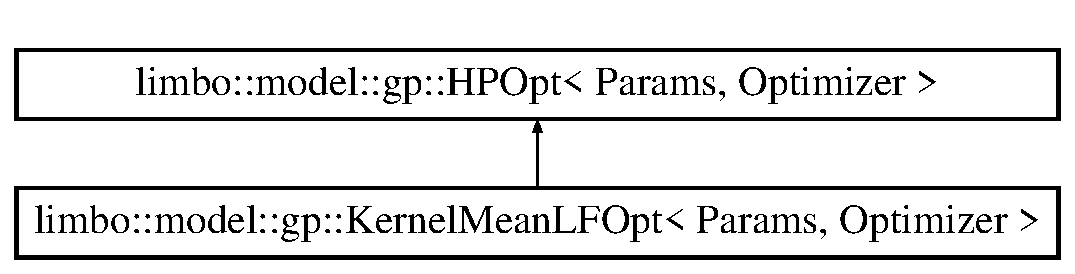
\includegraphics[height=2.000000cm]{structlimbo_1_1model_1_1gp_1_1_kernel_mean_l_f_opt}
\end{center}
\end{figure}
\subsection*{Public Member Functions}
\begin{DoxyCompactItemize}
\item 
{\footnotesize template$<$typename GP $>$ }\\void \hyperlink{structlimbo_1_1model_1_1gp_1_1_kernel_mean_l_f_opt_afdd30bef6dbad7b8f6e459bcea7f4412}{operator()} (\hyperlink{classlimbo_1_1model_1_1_g_p}{GP} \&gp)
\end{DoxyCompactItemize}


\subsection{Detailed Description}
\subsubsection*{template$<$typename Params, typename Optimizer = opt\+::\+Parallel\+Repeater$<$\+Params, opt\+::\+Rprop$<$\+Params$>$$>$$>$\\*
struct limbo\+::model\+::gp\+::\+Kernel\+Mean\+L\+F\+Opt$<$ Params, Optimizer $>$}

optimize the likelihood of both the kernel and the mean (try to align the mean function) 

\subsection{Member Function Documentation}
\index{limbo\+::model\+::gp\+::\+Kernel\+Mean\+L\+F\+Opt@{limbo\+::model\+::gp\+::\+Kernel\+Mean\+L\+F\+Opt}!operator()@{operator()}}
\index{operator()@{operator()}!limbo\+::model\+::gp\+::\+Kernel\+Mean\+L\+F\+Opt@{limbo\+::model\+::gp\+::\+Kernel\+Mean\+L\+F\+Opt}}
\subsubsection[{\texorpdfstring{operator()(\+G\+P \&gp)}{operator()(GP &gp)}}]{\setlength{\rightskip}{0pt plus 5cm}template$<$typename Params , typename Optimizer  = opt\+::\+Parallel\+Repeater$<$\+Params, opt\+::\+Rprop$<$\+Params$>$$>$$>$ template$<$typename GP $>$ void {\bf limbo\+::model\+::gp\+::\+Kernel\+Mean\+L\+F\+Opt}$<$ Params, Optimizer $>$\+::operator() (
\begin{DoxyParamCaption}
\item[{{\bf GP} \&}]{gp}
\end{DoxyParamCaption}
)\hspace{0.3cm}{\ttfamily [inline]}}\hypertarget{structlimbo_1_1model_1_1gp_1_1_kernel_mean_l_f_opt_afdd30bef6dbad7b8f6e459bcea7f4412}{}\label{structlimbo_1_1model_1_1gp_1_1_kernel_mean_l_f_opt_afdd30bef6dbad7b8f6e459bcea7f4412}


The documentation for this struct was generated from the following file\+:\begin{DoxyCompactItemize}
\item 
/tmp/doc\+\_\+limbo/limbo/src/limbo/model/gp/\hyperlink{kernel__mean__lf__opt_8hpp}{kernel\+\_\+mean\+\_\+lf\+\_\+opt.\+hpp}\end{DoxyCompactItemize}

\hypertarget{structlimbo_1_1kernel_1_1_matern_five_halves}{}\section{limbo\+:\+:kernel\+:\+:Matern\+Five\+Halves$<$ Params $>$ Struct Template Reference}
\label{structlimbo_1_1kernel_1_1_matern_five_halves}\index{limbo\+::kernel\+::\+Matern\+Five\+Halves$<$ Params $>$@{limbo\+::kernel\+::\+Matern\+Five\+Halves$<$ Params $>$}}


{\ttfamily \#include $<$limbo/kernel/matern\+\_\+five\+\_\+halves.\+hpp$>$}

\subsection*{Public Member Functions}
\begin{DoxyCompactItemize}
\item 
\hyperlink{structlimbo_1_1kernel_1_1_matern_five_halves_ad574e55051fb4728271945cb46ea11f0}{Matern\+Five\+Halves} (size\+\_\+t dim=1)
\item 
double \hyperlink{structlimbo_1_1kernel_1_1_matern_five_halves_a2949874230e0cd3f8116de67c3824987}{operator()} (const Eigen\+::\+Vector\+Xd \&v1, const Eigen\+::\+Vector\+Xd \&v2) const 
\end{DoxyCompactItemize}


\subsection{Detailed Description}
\subsubsection*{template$<$typename Params$>$\\*
struct limbo\+::kernel\+::\+Matern\+Five\+Halves$<$ Params $>$}

\begin{DoxyVerb}embed:rst

Matern kernel

.. math::
  d = ||v1 - v2||

  \nu = 5/2

  C(d) = \sigma^2\frac{2^{1-\nu}}{\Gamma(\nu)}\Bigg(\sqrt{2\nu}\frac{d}{l}\Bigg)^\nu K_\nu\Bigg(\sqrt{2\nu}\frac{d}{l}\Bigg),


Parameters:
  - ``double sigma_sq`` (signal variance)
  - ``double l`` (characteristic length scale)

Reference: :cite:`matern1960spatial` & :cite:`brochu2010tutorial` p.10 & https://en.wikipedia.org/wiki/Mat%C3%A9rn_covariance_function
\end{DoxyVerb}
 

\subsection{Constructor \& Destructor Documentation}
\index{limbo\+::kernel\+::\+Matern\+Five\+Halves@{limbo\+::kernel\+::\+Matern\+Five\+Halves}!Matern\+Five\+Halves@{Matern\+Five\+Halves}}
\index{Matern\+Five\+Halves@{Matern\+Five\+Halves}!limbo\+::kernel\+::\+Matern\+Five\+Halves@{limbo\+::kernel\+::\+Matern\+Five\+Halves}}
\subsubsection[{\texorpdfstring{Matern\+Five\+Halves(size\+\_\+t dim=1)}{MaternFiveHalves(size_t dim=1)}}]{\setlength{\rightskip}{0pt plus 5cm}template$<$typename Params $>$ {\bf limbo\+::kernel\+::\+Matern\+Five\+Halves}$<$ Params $>$\+::{\bf Matern\+Five\+Halves} (
\begin{DoxyParamCaption}
\item[{size\+\_\+t}]{dim = {\ttfamily 1}}
\end{DoxyParamCaption}
)\hspace{0.3cm}{\ttfamily [inline]}}\hypertarget{structlimbo_1_1kernel_1_1_matern_five_halves_ad574e55051fb4728271945cb46ea11f0}{}\label{structlimbo_1_1kernel_1_1_matern_five_halves_ad574e55051fb4728271945cb46ea11f0}


\subsection{Member Function Documentation}
\index{limbo\+::kernel\+::\+Matern\+Five\+Halves@{limbo\+::kernel\+::\+Matern\+Five\+Halves}!operator()@{operator()}}
\index{operator()@{operator()}!limbo\+::kernel\+::\+Matern\+Five\+Halves@{limbo\+::kernel\+::\+Matern\+Five\+Halves}}
\subsubsection[{\texorpdfstring{operator()(const Eigen\+::\+Vector\+Xd \&v1, const Eigen\+::\+Vector\+Xd \&v2) const }{operator()(const Eigen::VectorXd &v1, const Eigen::VectorXd &v2) const }}]{\setlength{\rightskip}{0pt plus 5cm}template$<$typename Params $>$ double {\bf limbo\+::kernel\+::\+Matern\+Five\+Halves}$<$ Params $>$\+::operator() (
\begin{DoxyParamCaption}
\item[{const Eigen\+::\+Vector\+Xd \&}]{v1, }
\item[{const Eigen\+::\+Vector\+Xd \&}]{v2}
\end{DoxyParamCaption}
) const\hspace{0.3cm}{\ttfamily [inline]}}\hypertarget{structlimbo_1_1kernel_1_1_matern_five_halves_a2949874230e0cd3f8116de67c3824987}{}\label{structlimbo_1_1kernel_1_1_matern_five_halves_a2949874230e0cd3f8116de67c3824987}


The documentation for this struct was generated from the following file\+:\begin{DoxyCompactItemize}
\item 
/tmp/doc\+\_\+limbo/limbo/src/limbo/kernel/\hyperlink{matern__five__halves_8hpp}{matern\+\_\+five\+\_\+halves.\+hpp}\end{DoxyCompactItemize}

\hypertarget{structlimbo_1_1kernel_1_1_matern_three_halves}{}\section{limbo\+:\+:kernel\+:\+:Matern\+Three\+Halves$<$ Params $>$ Struct Template Reference}
\label{structlimbo_1_1kernel_1_1_matern_three_halves}\index{limbo\+::kernel\+::\+Matern\+Three\+Halves$<$ Params $>$@{limbo\+::kernel\+::\+Matern\+Three\+Halves$<$ Params $>$}}


{\ttfamily \#include $<$limbo/kernel/matern\+\_\+three\+\_\+halves.\+hpp$>$}

\subsection*{Public Member Functions}
\begin{DoxyCompactItemize}
\item 
\hyperlink{structlimbo_1_1kernel_1_1_matern_three_halves_a676c205ada09d0ef4ba9ea36d68ba9b9}{Matern\+Three\+Halves} (size\+\_\+t dim=1)
\item 
double \hyperlink{structlimbo_1_1kernel_1_1_matern_three_halves_a9df77c86c2de097bed64edf38a721bb1}{operator()} (const Eigen\+::\+Vector\+Xd \&v1, const Eigen\+::\+Vector\+Xd \&v2) const 
\end{DoxyCompactItemize}


\subsection{Detailed Description}
\subsubsection*{template$<$typename Params$>$\\*
struct limbo\+::kernel\+::\+Matern\+Three\+Halves$<$ Params $>$}

\begin{DoxyVerb}embed:rst
 Matern 3/2 kernel

 .. math::
   d = ||v1 - v2||

   \nu = 3/2

   C(d) = \sigma^2\frac{2^{1-\nu}}{\Gamma(\nu)}\Bigg(\sqrt{2\nu}\frac{d}{l}\Bigg)^\nu K_\nu\Bigg(\sqrt{2\nu}\frac{d}{l}\Bigg),


 Parameters:
  - ``double sigma_sq`` (signal variance)
  - ``double l`` (characteristic length scale)

Reference: :cite:`matern1960spatial` & :cite:`brochu2010tutorial` p.10 & https://en.wikipedia.org/wiki/Mat%C3%A9rn_covariance_function
\end{DoxyVerb}
 

\subsection{Constructor \& Destructor Documentation}
\index{limbo\+::kernel\+::\+Matern\+Three\+Halves@{limbo\+::kernel\+::\+Matern\+Three\+Halves}!Matern\+Three\+Halves@{Matern\+Three\+Halves}}
\index{Matern\+Three\+Halves@{Matern\+Three\+Halves}!limbo\+::kernel\+::\+Matern\+Three\+Halves@{limbo\+::kernel\+::\+Matern\+Three\+Halves}}
\subsubsection[{\texorpdfstring{Matern\+Three\+Halves(size\+\_\+t dim=1)}{MaternThreeHalves(size_t dim=1)}}]{\setlength{\rightskip}{0pt plus 5cm}template$<$typename Params $>$ {\bf limbo\+::kernel\+::\+Matern\+Three\+Halves}$<$ Params $>$\+::{\bf Matern\+Three\+Halves} (
\begin{DoxyParamCaption}
\item[{size\+\_\+t}]{dim = {\ttfamily 1}}
\end{DoxyParamCaption}
)\hspace{0.3cm}{\ttfamily [inline]}}\hypertarget{structlimbo_1_1kernel_1_1_matern_three_halves_a676c205ada09d0ef4ba9ea36d68ba9b9}{}\label{structlimbo_1_1kernel_1_1_matern_three_halves_a676c205ada09d0ef4ba9ea36d68ba9b9}


\subsection{Member Function Documentation}
\index{limbo\+::kernel\+::\+Matern\+Three\+Halves@{limbo\+::kernel\+::\+Matern\+Three\+Halves}!operator()@{operator()}}
\index{operator()@{operator()}!limbo\+::kernel\+::\+Matern\+Three\+Halves@{limbo\+::kernel\+::\+Matern\+Three\+Halves}}
\subsubsection[{\texorpdfstring{operator()(const Eigen\+::\+Vector\+Xd \&v1, const Eigen\+::\+Vector\+Xd \&v2) const }{operator()(const Eigen::VectorXd &v1, const Eigen::VectorXd &v2) const }}]{\setlength{\rightskip}{0pt plus 5cm}template$<$typename Params $>$ double {\bf limbo\+::kernel\+::\+Matern\+Three\+Halves}$<$ Params $>$\+::operator() (
\begin{DoxyParamCaption}
\item[{const Eigen\+::\+Vector\+Xd \&}]{v1, }
\item[{const Eigen\+::\+Vector\+Xd \&}]{v2}
\end{DoxyParamCaption}
) const\hspace{0.3cm}{\ttfamily [inline]}}\hypertarget{structlimbo_1_1kernel_1_1_matern_three_halves_a9df77c86c2de097bed64edf38a721bb1}{}\label{structlimbo_1_1kernel_1_1_matern_three_halves_a9df77c86c2de097bed64edf38a721bb1}


The documentation for this struct was generated from the following file\+:\begin{DoxyCompactItemize}
\item 
/tmp/doc\+\_\+limbo/limbo/src/limbo/kernel/\hyperlink{matern__three__halves_8hpp}{matern\+\_\+three\+\_\+halves.\+hpp}\end{DoxyCompactItemize}

\hypertarget{structlimbo_1_1stop_1_1_max_iterations}{}\section{limbo\+:\+:stop\+:\+:Max\+Iterations$<$ Params $>$ Struct Template Reference}
\label{structlimbo_1_1stop_1_1_max_iterations}\index{limbo\+::stop\+::\+Max\+Iterations$<$ Params $>$@{limbo\+::stop\+::\+Max\+Iterations$<$ Params $>$}}


{\ttfamily \#include $<$limbo/stop/max\+\_\+iterations.\+hpp$>$}

\subsection*{Public Member Functions}
\begin{DoxyCompactItemize}
\item 
\hyperlink{structlimbo_1_1stop_1_1_max_iterations_a07bb1bbffe6b7374c9d1af7575dbc745}{Max\+Iterations} ()
\item 
{\footnotesize template$<$typename BO , typename Aggregator\+Function $>$ }\\bool \hyperlink{structlimbo_1_1stop_1_1_max_iterations_a357c80242e43d6cd25e48a63044bf2a2}{operator()} (const BO \&bo, const Aggregator\+Function \&)
\end{DoxyCompactItemize}


\subsection{Detailed Description}
\subsubsection*{template$<$typename Params$>$\\*
struct limbo\+::stop\+::\+Max\+Iterations$<$ Params $>$}

Stop after a given number of iterations

parameter\+: int iterations 

\subsection{Constructor \& Destructor Documentation}
\index{limbo\+::stop\+::\+Max\+Iterations@{limbo\+::stop\+::\+Max\+Iterations}!Max\+Iterations@{Max\+Iterations}}
\index{Max\+Iterations@{Max\+Iterations}!limbo\+::stop\+::\+Max\+Iterations@{limbo\+::stop\+::\+Max\+Iterations}}
\subsubsection[{\texorpdfstring{Max\+Iterations()}{MaxIterations()}}]{\setlength{\rightskip}{0pt plus 5cm}template$<$typename Params $>$ {\bf limbo\+::stop\+::\+Max\+Iterations}$<$ Params $>$\+::{\bf Max\+Iterations} (
\begin{DoxyParamCaption}
{}
\end{DoxyParamCaption}
)\hspace{0.3cm}{\ttfamily [inline]}}\hypertarget{structlimbo_1_1stop_1_1_max_iterations_a07bb1bbffe6b7374c9d1af7575dbc745}{}\label{structlimbo_1_1stop_1_1_max_iterations_a07bb1bbffe6b7374c9d1af7575dbc745}


\subsection{Member Function Documentation}
\index{limbo\+::stop\+::\+Max\+Iterations@{limbo\+::stop\+::\+Max\+Iterations}!operator()@{operator()}}
\index{operator()@{operator()}!limbo\+::stop\+::\+Max\+Iterations@{limbo\+::stop\+::\+Max\+Iterations}}
\subsubsection[{\texorpdfstring{operator()(const B\+O \&bo, const Aggregator\+Function \&)}{operator()(const BO &bo, const AggregatorFunction &)}}]{\setlength{\rightskip}{0pt plus 5cm}template$<$typename Params $>$ template$<$typename BO , typename Aggregator\+Function $>$ bool {\bf limbo\+::stop\+::\+Max\+Iterations}$<$ Params $>$\+::operator() (
\begin{DoxyParamCaption}
\item[{const BO \&}]{bo, }
\item[{const Aggregator\+Function \&}]{}
\end{DoxyParamCaption}
)\hspace{0.3cm}{\ttfamily [inline]}}\hypertarget{structlimbo_1_1stop_1_1_max_iterations_a357c80242e43d6cd25e48a63044bf2a2}{}\label{structlimbo_1_1stop_1_1_max_iterations_a357c80242e43d6cd25e48a63044bf2a2}


The documentation for this struct was generated from the following file\+:\begin{DoxyCompactItemize}
\item 
/tmp/doc\+\_\+limbo/limbo/src/limbo/stop/\hyperlink{max__iterations_8hpp}{max\+\_\+iterations.\+hpp}\end{DoxyCompactItemize}

\hypertarget{structlimbo_1_1stop_1_1_max_predicted_value}{}\section{limbo\+:\+:stop\+:\+:Max\+Predicted\+Value$<$ Params, Optimizer $>$ Struct Template Reference}
\label{structlimbo_1_1stop_1_1_max_predicted_value}\index{limbo\+::stop\+::\+Max\+Predicted\+Value$<$ Params, Optimizer $>$@{limbo\+::stop\+::\+Max\+Predicted\+Value$<$ Params, Optimizer $>$}}


{\ttfamily \#include $<$limbo/stop/max\+\_\+predicted\+\_\+value.\+hpp$>$}

\subsection*{Public Member Functions}
\begin{DoxyCompactItemize}
\item 
\hyperlink{structlimbo_1_1stop_1_1_max_predicted_value_a211e3d4d8935c84ddb27e09d76a1726a}{Max\+Predicted\+Value} ()
\item 
{\footnotesize template$<$typename BO , typename Aggregator\+Function $>$ }\\bool \hyperlink{structlimbo_1_1stop_1_1_max_predicted_value_a7f5cb07d4a9b666e4c1cac91afa3fca0}{operator()} (const BO \&bo, const Aggregator\+Function \&afun) const 
\end{DoxyCompactItemize}


\subsection{Detailed Description}
\subsubsection*{template$<$typename Params, typename Optimizer = boost\+::parameter\+::void\+\_\+$>$\\*
struct limbo\+::stop\+::\+Max\+Predicted\+Value$<$ Params, Optimizer $>$}

Stop once the value for the best sample is above \+: ratio $\ast$ (best value predicted by the model)

Parameter\+: double ratio 

\subsection{Constructor \& Destructor Documentation}
\index{limbo\+::stop\+::\+Max\+Predicted\+Value@{limbo\+::stop\+::\+Max\+Predicted\+Value}!Max\+Predicted\+Value@{Max\+Predicted\+Value}}
\index{Max\+Predicted\+Value@{Max\+Predicted\+Value}!limbo\+::stop\+::\+Max\+Predicted\+Value@{limbo\+::stop\+::\+Max\+Predicted\+Value}}
\subsubsection[{\texorpdfstring{Max\+Predicted\+Value()}{MaxPredictedValue()}}]{\setlength{\rightskip}{0pt plus 5cm}template$<$typename Params , typename Optimizer  = boost\+::parameter\+::void\+\_\+$>$ {\bf limbo\+::stop\+::\+Max\+Predicted\+Value}$<$ Params, Optimizer $>$\+::{\bf Max\+Predicted\+Value} (
\begin{DoxyParamCaption}
{}
\end{DoxyParamCaption}
)\hspace{0.3cm}{\ttfamily [inline]}}\hypertarget{structlimbo_1_1stop_1_1_max_predicted_value_a211e3d4d8935c84ddb27e09d76a1726a}{}\label{structlimbo_1_1stop_1_1_max_predicted_value_a211e3d4d8935c84ddb27e09d76a1726a}


\subsection{Member Function Documentation}
\index{limbo\+::stop\+::\+Max\+Predicted\+Value@{limbo\+::stop\+::\+Max\+Predicted\+Value}!operator()@{operator()}}
\index{operator()@{operator()}!limbo\+::stop\+::\+Max\+Predicted\+Value@{limbo\+::stop\+::\+Max\+Predicted\+Value}}
\subsubsection[{\texorpdfstring{operator()(const B\+O \&bo, const Aggregator\+Function \&afun) const }{operator()(const BO &bo, const AggregatorFunction &afun) const }}]{\setlength{\rightskip}{0pt plus 5cm}template$<$typename Params , typename Optimizer  = boost\+::parameter\+::void\+\_\+$>$ template$<$typename BO , typename Aggregator\+Function $>$ bool {\bf limbo\+::stop\+::\+Max\+Predicted\+Value}$<$ Params, Optimizer $>$\+::operator() (
\begin{DoxyParamCaption}
\item[{const BO \&}]{bo, }
\item[{const Aggregator\+Function \&}]{afun}
\end{DoxyParamCaption}
) const\hspace{0.3cm}{\ttfamily [inline]}}\hypertarget{structlimbo_1_1stop_1_1_max_predicted_value_a7f5cb07d4a9b666e4c1cac91afa3fca0}{}\label{structlimbo_1_1stop_1_1_max_predicted_value_a7f5cb07d4a9b666e4c1cac91afa3fca0}


The documentation for this struct was generated from the following file\+:\begin{DoxyCompactItemize}
\item 
/tmp/doc\+\_\+limbo/limbo/src/limbo/stop/\hyperlink{max__predicted__value_8hpp}{max\+\_\+predicted\+\_\+value.\+hpp}\end{DoxyCompactItemize}

\hypertarget{structlimbo_1_1defaults_1_1mean__constant}{}\section{limbo\+:\+:defaults\+:\+:mean\+\_\+constant Struct Reference}
\label{structlimbo_1_1defaults_1_1mean__constant}\index{limbo\+::defaults\+::mean\+\_\+constant@{limbo\+::defaults\+::mean\+\_\+constant}}


{\ttfamily \#include $<$limbo/mean/constant.\+hpp$>$}

\subsection*{Public Member Functions}
\begin{DoxyCompactItemize}
\item 
\hyperlink{group__mean__defaults_gafa1b143b975c61c4547a005794f44a12}{B\+O\+\_\+\+P\+A\+R\+AM} (double, constant, 1)
\end{DoxyCompactItemize}


The documentation for this struct was generated from the following file\+:\begin{DoxyCompactItemize}
\item 
/tmp/doc\+\_\+limbo/limbo/src/limbo/mean/\hyperlink{constant_8hpp}{constant.\+hpp}\end{DoxyCompactItemize}

\hypertarget{structlimbo_1_1model_1_1gp_1_1_mean_l_f_opt}{}\section{limbo\+:\+:model\+:\+:gp\+:\+:Mean\+L\+F\+Opt$<$ Params, Optimizer $>$ Struct Template Reference}
\label{structlimbo_1_1model_1_1gp_1_1_mean_l_f_opt}\index{limbo\+::model\+::gp\+::\+Mean\+L\+F\+Opt$<$ Params, Optimizer $>$@{limbo\+::model\+::gp\+::\+Mean\+L\+F\+Opt$<$ Params, Optimizer $>$}}


{\ttfamily \#include $<$limbo/model/gp/mean\+\_\+lf\+\_\+opt.\+hpp$>$}

Inheritance diagram for limbo\+:\+:model\+:\+:gp\+:\+:Mean\+L\+F\+Opt$<$ Params, Optimizer $>$\+:\begin{figure}[H]
\begin{center}
\leavevmode
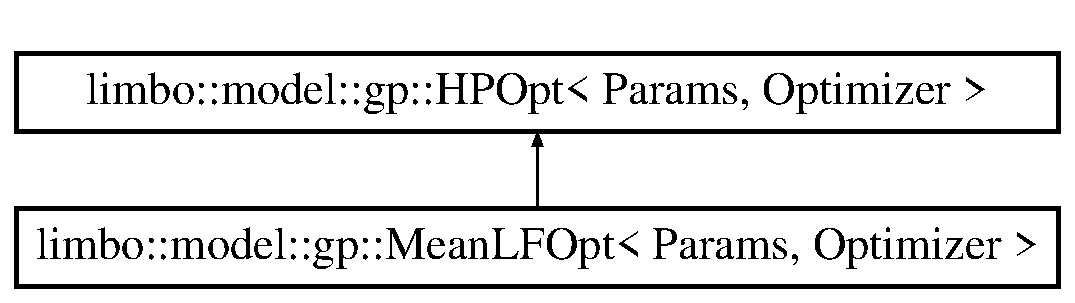
\includegraphics[height=2.000000cm]{structlimbo_1_1model_1_1gp_1_1_mean_l_f_opt}
\end{center}
\end{figure}
\subsection*{Public Member Functions}
\begin{DoxyCompactItemize}
\item 
{\footnotesize template$<$typename G\+P $>$ }\\void \hyperlink{structlimbo_1_1model_1_1gp_1_1_mean_l_f_opt_a3db7aa510b906aeacc851f984ceac1ca}{operator()} (\hyperlink{classlimbo_1_1model_1_1_g_p}{G\+P} \&gp)
\end{DoxyCompactItemize}


\subsection{Detailed Description}
\subsubsection*{template$<$typename Params, typename Optimizer = opt\+::\+Parallel\+Repeater$<$\+Params, opt\+::\+Rprop$<$\+Params$>$$>$$>$struct limbo\+::model\+::gp\+::\+Mean\+L\+F\+Opt$<$ Params, Optimizer $>$}

optimize the likelihood of the mean only (try to align the mean function) 

\subsection{Member Function Documentation}
\hypertarget{structlimbo_1_1model_1_1gp_1_1_mean_l_f_opt_a3db7aa510b906aeacc851f984ceac1ca}{}\index{limbo\+::model\+::gp\+::\+Mean\+L\+F\+Opt@{limbo\+::model\+::gp\+::\+Mean\+L\+F\+Opt}!operator()@{operator()}}
\index{operator()@{operator()}!limbo\+::model\+::gp\+::\+Mean\+L\+F\+Opt@{limbo\+::model\+::gp\+::\+Mean\+L\+F\+Opt}}
\subsubsection[{operator()}]{\setlength{\rightskip}{0pt plus 5cm}template$<$typename Params , typename Optimizer  = opt\+::\+Parallel\+Repeater$<$\+Params, opt\+::\+Rprop$<$\+Params$>$$>$$>$ template$<$typename G\+P $>$ void {\bf limbo\+::model\+::gp\+::\+Mean\+L\+F\+Opt}$<$ Params, Optimizer $>$\+::operator() (
\begin{DoxyParamCaption}
\item[{{\bf G\+P} \&}]{gp}
\end{DoxyParamCaption}
)\hspace{0.3cm}{\ttfamily [inline]}}\label{structlimbo_1_1model_1_1gp_1_1_mean_l_f_opt_a3db7aa510b906aeacc851f984ceac1ca}


The documentation for this struct was generated from the following file\+:\begin{DoxyCompactItemize}
\item 
/tmp/doc\+\_\+limbo/limbo/src/limbo/model/gp/\hyperlink{mean__lf__opt_8hpp}{mean\+\_\+lf\+\_\+opt.\+hpp}\end{DoxyCompactItemize}

\hypertarget{structlimbo_1_1experimental_1_1defaults_1_1model__gp__parego}{}\section{limbo\+:\+:experimental\+:\+:defaults\+:\+:model\+\_\+gp\+\_\+parego Struct Reference}
\label{structlimbo_1_1experimental_1_1defaults_1_1model__gp__parego}\index{limbo\+::experimental\+::defaults\+::model\+\_\+gp\+\_\+parego@{limbo\+::experimental\+::defaults\+::model\+\_\+gp\+\_\+parego}}


{\ttfamily \#include $<$limbo/experimental/model/gp\+\_\+parego.\+hpp$>$}

\subsection*{Public Member Functions}
\begin{DoxyCompactItemize}
\item 
\hyperlink{structlimbo_1_1experimental_1_1defaults_1_1model__gp__parego_ad284d6ed4055b749d2257383a66159f7}{B\+O\+\_\+\+P\+A\+R\+A\+M} (double, rho, 0.\+05)
\end{DoxyCompactItemize}


\subsection{Member Function Documentation}
\hypertarget{structlimbo_1_1experimental_1_1defaults_1_1model__gp__parego_ad284d6ed4055b749d2257383a66159f7}{}\index{limbo\+::experimental\+::defaults\+::model\+\_\+gp\+\_\+parego@{limbo\+::experimental\+::defaults\+::model\+\_\+gp\+\_\+parego}!B\+O\+\_\+\+P\+A\+R\+A\+M@{B\+O\+\_\+\+P\+A\+R\+A\+M}}
\index{B\+O\+\_\+\+P\+A\+R\+A\+M@{B\+O\+\_\+\+P\+A\+R\+A\+M}!limbo\+::experimental\+::defaults\+::model\+\_\+gp\+\_\+parego@{limbo\+::experimental\+::defaults\+::model\+\_\+gp\+\_\+parego}}
\subsubsection[{B\+O\+\_\+\+P\+A\+R\+A\+M}]{\setlength{\rightskip}{0pt plus 5cm}limbo\+::experimental\+::defaults\+::model\+\_\+gp\+\_\+parego\+::\+B\+O\+\_\+\+P\+A\+R\+A\+M (
\begin{DoxyParamCaption}
\item[{double}]{, }
\item[{rho}]{, }
\item[{0.}]{05}
\end{DoxyParamCaption}
)}\label{structlimbo_1_1experimental_1_1defaults_1_1model__gp__parego_ad284d6ed4055b749d2257383a66159f7}


The documentation for this struct was generated from the following file\+:\begin{DoxyCompactItemize}
\item 
/tmp/doc\+\_\+limbo/limbo/src/limbo/experimental/model/\hyperlink{gp__parego_8hpp}{gp\+\_\+parego.\+hpp}\end{DoxyCompactItemize}

\hypertarget{structlimbo_1_1opt_1_1_n_l_opt_grad}{}\section{limbo\+:\+:opt\+:\+:N\+L\+Opt\+Grad$<$ Params, Algorithm $>$ Struct Template Reference}
\label{structlimbo_1_1opt_1_1_n_l_opt_grad}\index{limbo\+::opt\+::\+N\+L\+Opt\+Grad$<$ Params, Algorithm $>$@{limbo\+::opt\+::\+N\+L\+Opt\+Grad$<$ Params, Algorithm $>$}}


{\ttfamily \#include $<$limbo/opt/nlopt\+\_\+grad.\+hpp$>$}

\subsection*{Public Member Functions}
\begin{DoxyCompactItemize}
\item 
{\footnotesize template$<$typename F $>$ }\\Eigen\+::\+Vector\+Xd \hyperlink{structlimbo_1_1opt_1_1_n_l_opt_grad_a248805060cc986c4553d91f738b8b725}{operator()} (const F \&f, const Eigen\+::\+Vector\+Xd \&init, bool bounded) const 
\end{DoxyCompactItemize}


\subsection{Detailed Description}
\subsubsection*{template$<$typename Params, nlopt\+::algorithm Algorithm = nlopt\+::\+L\+D\+\_\+\+L\+B\+F\+GS$>$\\*
struct limbo\+::opt\+::\+N\+L\+Opt\+Grad$<$ Params, Algorithm $>$}

Binding to gradient-\/based N\+L\+Opt algorithms. See\+: \href{http://ab-initio.mit.edu/wiki/index.php/NLopt_Algorithms}{\tt http\+://ab-\/initio.\+mit.\+edu/wiki/index.\+php/\+N\+Lopt\+\_\+\+Algorithms}

Algorithms\+:
\begin{DoxyItemize}
\item G\+D\+\_\+\+S\+T\+O\+GO
\item G\+D\+\_\+\+S\+T\+O\+G\+O\+\_\+\+R\+A\+ND
\item L\+D\+\_\+\+L\+B\+F\+G\+S\+\_\+\+N\+O\+C\+E\+D\+AL
\item L\+D\+\_\+\+L\+B\+F\+GS
\item L\+N\+\_\+\+P\+R\+A\+X\+IS
\item L\+D\+\_\+\+V\+A\+R1
\item L\+D\+\_\+\+V\+A\+R2
\item L\+D\+\_\+\+T\+N\+E\+W\+T\+ON
\item L\+D\+\_\+\+T\+N\+E\+W\+T\+O\+N\+\_\+\+R\+E\+S\+T\+A\+RT
\item L\+D\+\_\+\+T\+N\+E\+W\+T\+O\+N\+\_\+\+P\+R\+E\+C\+O\+ND
\item L\+D\+\_\+\+T\+N\+E\+W\+T\+O\+N\+\_\+\+P\+R\+E\+C\+O\+N\+D\+\_\+\+R\+E\+S\+T\+A\+RT
\item G\+D\+\_\+\+M\+L\+SL
\item G\+N\+\_\+\+M\+L\+S\+L\+\_\+\+L\+DS
\item G\+D\+\_\+\+M\+L\+S\+L\+\_\+\+L\+DS
\item L\+D\+\_\+\+M\+MA
\item L\+D\+\_\+\+A\+U\+G\+L\+AG
\item L\+D\+\_\+\+A\+U\+G\+L\+A\+G\+\_\+\+EQ
\item L\+D\+\_\+\+S\+L\+S\+QP
\item L\+D\+\_\+\+C\+C\+S\+AQ
\end{DoxyItemize}

Parameters \+:
\begin{DoxyItemize}
\item int iterations 
\end{DoxyItemize}

\subsection{Member Function Documentation}
\index{limbo\+::opt\+::\+N\+L\+Opt\+Grad@{limbo\+::opt\+::\+N\+L\+Opt\+Grad}!operator()@{operator()}}
\index{operator()@{operator()}!limbo\+::opt\+::\+N\+L\+Opt\+Grad@{limbo\+::opt\+::\+N\+L\+Opt\+Grad}}
\subsubsection[{\texorpdfstring{operator()(const F \&f, const Eigen\+::\+Vector\+Xd \&init, bool bounded) const }{operator()(const F &f, const Eigen::VectorXd &init, bool bounded) const }}]{\setlength{\rightskip}{0pt plus 5cm}template$<$typename Params , nlopt\+::algorithm Algorithm = nlopt\+::\+L\+D\+\_\+\+L\+B\+F\+GS$>$ template$<$typename F $>$ Eigen\+::\+Vector\+Xd {\bf limbo\+::opt\+::\+N\+L\+Opt\+Grad}$<$ Params, Algorithm $>$\+::operator() (
\begin{DoxyParamCaption}
\item[{const F \&}]{f, }
\item[{const Eigen\+::\+Vector\+Xd \&}]{init, }
\item[{bool}]{bounded}
\end{DoxyParamCaption}
) const\hspace{0.3cm}{\ttfamily [inline]}}\hypertarget{structlimbo_1_1opt_1_1_n_l_opt_grad_a248805060cc986c4553d91f738b8b725}{}\label{structlimbo_1_1opt_1_1_n_l_opt_grad_a248805060cc986c4553d91f738b8b725}


The documentation for this struct was generated from the following file\+:\begin{DoxyCompactItemize}
\item 
/tmp/doc\+\_\+limbo/limbo/src/limbo/opt/\hyperlink{nlopt__grad_8hpp}{nlopt\+\_\+grad.\+hpp}\end{DoxyCompactItemize}

\hypertarget{structlimbo_1_1opt_1_1_n_l_opt_no_grad}{}\section{limbo\+:\+:opt\+:\+:N\+L\+Opt\+No\+Grad$<$ Params, Algorithm $>$ Struct Template Reference}
\label{structlimbo_1_1opt_1_1_n_l_opt_no_grad}\index{limbo\+::opt\+::\+N\+L\+Opt\+No\+Grad$<$ Params, Algorithm $>$@{limbo\+::opt\+::\+N\+L\+Opt\+No\+Grad$<$ Params, Algorithm $>$}}


{\ttfamily \#include $<$limbo/opt/nlopt\+\_\+no\+\_\+grad.\+hpp$>$}

\subsection*{Public Member Functions}
\begin{DoxyCompactItemize}
\item 
{\footnotesize template$<$typename F $>$ }\\Eigen\+::\+Vector\+Xd \hyperlink{structlimbo_1_1opt_1_1_n_l_opt_no_grad_a23cdeb4f9c63e44bd7fb4dbf8d8553d7}{operator()} (const F \&f, const Eigen\+::\+Vector\+Xd \&init, bool bounded) const 
\end{DoxyCompactItemize}


\subsection{Detailed Description}
\subsubsection*{template$<$typename Params, nlopt\+::algorithm Algorithm = nlopt\+::\+G\+N\+\_\+\+D\+I\+R\+E\+C\+T\+\_\+\+L\+\_\+\+R\+A\+N\+D$>$struct limbo\+::opt\+::\+N\+L\+Opt\+No\+Grad$<$ Params, Algorithm $>$}

Binding to gradient-\/free N\+L\+Opt algorithms. See\+: \href{http://ab-initio.mit.edu/wiki/index.php/NLopt_Algorithms}{\tt http\+://ab-\/initio.\+mit.\+edu/wiki/index.\+php/\+N\+Lopt\+\_\+\+Algorithms}

Algorithms\+:
\begin{DoxyItemize}
\item G\+N\+\_\+\+D\+I\+R\+E\+C\+T
\item G\+N\+\_\+\+D\+I\+R\+E\+C\+T\+\_\+\+L, \mbox{[}default\mbox{]}
\item G\+N\+\_\+\+D\+I\+R\+E\+C\+T\+\_\+\+L\+\_\+\+R\+A\+N\+D
\item G\+N\+\_\+\+D\+I\+R\+E\+C\+T\+\_\+\+N\+O\+S\+C\+A\+L
\item G\+N\+\_\+\+D\+I\+R\+E\+C\+T\+\_\+\+L\+\_\+\+N\+O\+S\+C\+A\+L
\item G\+N\+\_\+\+D\+I\+R\+E\+C\+T\+\_\+\+L\+\_\+\+R\+A\+N\+D\+\_\+\+N\+O\+S\+C\+A\+L
\item G\+N\+\_\+\+O\+R\+I\+G\+\_\+\+D\+I\+R\+E\+C\+T
\item G\+N\+\_\+\+O\+R\+I\+G\+\_\+\+D\+I\+R\+E\+C\+T\+\_\+\+L
\item G\+N\+\_\+\+C\+R\+S2\+\_\+\+L\+M
\item G\+N\+\_\+\+M\+L\+S\+L
\item G\+N\+\_\+\+M\+L\+S\+L\+\_\+\+L\+D\+S
\item G\+N\+\_\+\+I\+S\+R\+E\+S
\item L\+N\+\_\+\+C\+O\+B\+Y\+L\+A
\item L\+N\+\_\+\+A\+U\+G\+L\+A\+G\+\_\+\+E\+Q
\item L\+N\+\_\+\+B\+O\+B\+Y\+Q\+A
\item L\+N\+\_\+\+N\+E\+W\+U\+O\+A
\item L\+N\+\_\+\+N\+E\+W\+U\+O\+A\+\_\+\+B\+O\+U\+N\+D
\item L\+N\+\_\+\+N\+E\+L\+D\+E\+R\+M\+E\+A\+D
\item L\+N\+\_\+\+S\+B\+P\+L\+X
\item L\+N\+\_\+\+A\+U\+G\+L\+A\+G
\end{DoxyItemize}

Parameters\+:
\begin{DoxyItemize}
\item int iterations 
\end{DoxyItemize}

\subsection{Member Function Documentation}
\hypertarget{structlimbo_1_1opt_1_1_n_l_opt_no_grad_a23cdeb4f9c63e44bd7fb4dbf8d8553d7}{}\index{limbo\+::opt\+::\+N\+L\+Opt\+No\+Grad@{limbo\+::opt\+::\+N\+L\+Opt\+No\+Grad}!operator()@{operator()}}
\index{operator()@{operator()}!limbo\+::opt\+::\+N\+L\+Opt\+No\+Grad@{limbo\+::opt\+::\+N\+L\+Opt\+No\+Grad}}
\subsubsection[{operator()}]{\setlength{\rightskip}{0pt plus 5cm}template$<$typename Params , nlopt\+::algorithm Algorithm = nlopt\+::\+G\+N\+\_\+\+D\+I\+R\+E\+C\+T\+\_\+\+L\+\_\+\+R\+A\+N\+D$>$ template$<$typename F $>$ Eigen\+::\+Vector\+Xd {\bf limbo\+::opt\+::\+N\+L\+Opt\+No\+Grad}$<$ Params, Algorithm $>$\+::operator() (
\begin{DoxyParamCaption}
\item[{const F \&}]{f, }
\item[{const Eigen\+::\+Vector\+Xd \&}]{init, }
\item[{bool}]{bounded}
\end{DoxyParamCaption}
) const\hspace{0.3cm}{\ttfamily [inline]}}\label{structlimbo_1_1opt_1_1_n_l_opt_no_grad_a23cdeb4f9c63e44bd7fb4dbf8d8553d7}


The documentation for this struct was generated from the following file\+:\begin{DoxyCompactItemize}
\item 
/tmp/doc\+\_\+limbo/limbo/src/limbo/opt/\hyperlink{nlopt__no__grad_8hpp}{nlopt\+\_\+no\+\_\+grad.\+hpp}\end{DoxyCompactItemize}

\hypertarget{structlimbo_1_1init_1_1_no_init}{}\section{limbo\+:\+:init\+:\+:No\+Init$<$ Params $>$ Struct Template Reference}
\label{structlimbo_1_1init_1_1_no_init}\index{limbo\+::init\+::\+No\+Init$<$ Params $>$@{limbo\+::init\+::\+No\+Init$<$ Params $>$}}


{\ttfamily \#include $<$limbo/init/no\+\_\+init.\+hpp$>$}

\subsection*{Public Member Functions}
\begin{DoxyCompactItemize}
\item 
{\footnotesize template$<$typename State\+Function , typename Aggregator\+Function , typename Opt $>$ }\\void \hyperlink{structlimbo_1_1init_1_1_no_init_a9fa7394b1924bd1f3f8f9f7d27d582ee}{operator()} (const State\+Function \&, const Aggregator\+Function \&, Opt \&) const 
\end{DoxyCompactItemize}


\subsection{Detailed Description}
\subsubsection*{template$<$typename Params$>$\\*
struct limbo\+::init\+::\+No\+Init$<$ Params $>$}

Do nothing (dummy initializer). 

\subsection{Member Function Documentation}
\index{limbo\+::init\+::\+No\+Init@{limbo\+::init\+::\+No\+Init}!operator()@{operator()}}
\index{operator()@{operator()}!limbo\+::init\+::\+No\+Init@{limbo\+::init\+::\+No\+Init}}
\subsubsection[{\texorpdfstring{operator()(const State\+Function \&, const Aggregator\+Function \&, Opt \&) const }{operator()(const StateFunction &, const AggregatorFunction &, Opt &) const }}]{\setlength{\rightskip}{0pt plus 5cm}template$<$typename Params $>$ template$<$typename State\+Function , typename Aggregator\+Function , typename Opt $>$ void {\bf limbo\+::init\+::\+No\+Init}$<$ Params $>$\+::operator() (
\begin{DoxyParamCaption}
\item[{const State\+Function \&}]{, }
\item[{const Aggregator\+Function \&}]{, }
\item[{Opt \&}]{}
\end{DoxyParamCaption}
) const\hspace{0.3cm}{\ttfamily [inline]}}\hypertarget{structlimbo_1_1init_1_1_no_init_a9fa7394b1924bd1f3f8f9f7d27d582ee}{}\label{structlimbo_1_1init_1_1_no_init_a9fa7394b1924bd1f3f8f9f7d27d582ee}


The documentation for this struct was generated from the following file\+:\begin{DoxyCompactItemize}
\item 
/tmp/doc\+\_\+limbo/limbo/src/limbo/init/\hyperlink{no__init_8hpp}{no\+\_\+init.\+hpp}\end{DoxyCompactItemize}

\hypertarget{structlimbo_1_1model_1_1gp_1_1_no_l_f_opt}{}\section{limbo\+:\+:model\+:\+:gp\+:\+:No\+L\+F\+Opt$<$ Params $>$ Struct Template Reference}
\label{structlimbo_1_1model_1_1gp_1_1_no_l_f_opt}\index{limbo\+::model\+::gp\+::\+No\+L\+F\+Opt$<$ Params $>$@{limbo\+::model\+::gp\+::\+No\+L\+F\+Opt$<$ Params $>$}}


{\ttfamily \#include $<$limbo/model/gp/no\+\_\+lf\+\_\+opt.\+hpp$>$}

\subsection*{Public Member Functions}
\begin{DoxyCompactItemize}
\item 
{\footnotesize template$<$typename GP $>$ }\\void \hyperlink{structlimbo_1_1model_1_1gp_1_1_no_l_f_opt_abeb1162ce0ee3cd307cdd22ded7986b6}{operator()} (\hyperlink{classlimbo_1_1model_1_1_g_p}{GP} \&) const 
\end{DoxyCompactItemize}


\subsection{Detailed Description}
\subsubsection*{template$<$typename Params$>$\\*
struct limbo\+::model\+::gp\+::\+No\+L\+F\+Opt$<$ Params $>$}

do not optimize anything 

\subsection{Member Function Documentation}
\index{limbo\+::model\+::gp\+::\+No\+L\+F\+Opt@{limbo\+::model\+::gp\+::\+No\+L\+F\+Opt}!operator()@{operator()}}
\index{operator()@{operator()}!limbo\+::model\+::gp\+::\+No\+L\+F\+Opt@{limbo\+::model\+::gp\+::\+No\+L\+F\+Opt}}
\subsubsection[{\texorpdfstring{operator()(\+G\+P \&) const }{operator()(GP &) const }}]{\setlength{\rightskip}{0pt plus 5cm}template$<$typename Params $>$ template$<$typename GP $>$ void {\bf limbo\+::model\+::gp\+::\+No\+L\+F\+Opt}$<$ Params $>$\+::operator() (
\begin{DoxyParamCaption}
\item[{{\bf GP} \&}]{}
\end{DoxyParamCaption}
) const\hspace{0.3cm}{\ttfamily [inline]}}\hypertarget{structlimbo_1_1model_1_1gp_1_1_no_l_f_opt_abeb1162ce0ee3cd307cdd22ded7986b6}{}\label{structlimbo_1_1model_1_1gp_1_1_no_l_f_opt_abeb1162ce0ee3cd307cdd22ded7986b6}


The documentation for this struct was generated from the following file\+:\begin{DoxyCompactItemize}
\item 
/tmp/doc\+\_\+limbo/limbo/src/limbo/model/gp/\hyperlink{no__lf__opt_8hpp}{no\+\_\+lf\+\_\+opt.\+hpp}\end{DoxyCompactItemize}

\hypertarget{classlimbo_1_1experimental_1_1bayes__opt_1_1_nsbo}{}\section{limbo\+:\+:experimental\+:\+:bayes\+\_\+opt\+:\+:Nsbo$<$ Params, A2, A3, A4, A5, A6 $>$ Class Template Reference}
\label{classlimbo_1_1experimental_1_1bayes__opt_1_1_nsbo}\index{limbo\+::experimental\+::bayes\+\_\+opt\+::\+Nsbo$<$ Params, A2, A3, A4, A5, A6 $>$@{limbo\+::experimental\+::bayes\+\_\+opt\+::\+Nsbo$<$ Params, A2, A3, A4, A5, A6 $>$}}


{\ttfamily \#include $<$limbo/experimental/bayes\+\_\+opt/nsbo.\+hpp$>$}

Inheritance diagram for limbo\+:\+:experimental\+:\+:bayes\+\_\+opt\+:\+:Nsbo$<$ Params, A2, A3, A4, A5, A6 $>$\+:\begin{figure}[H]
\begin{center}
\leavevmode
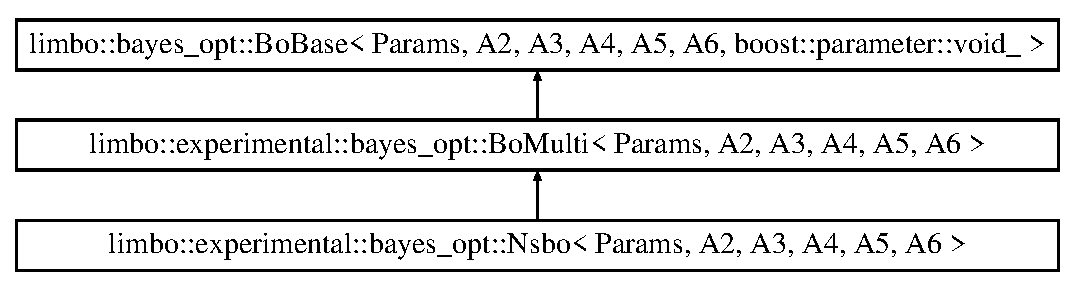
\includegraphics[height=3.000000cm]{classlimbo_1_1experimental_1_1bayes__opt_1_1_nsbo}
\end{center}
\end{figure}
\subsection*{Public Types}
\begin{DoxyCompactItemize}
\item 
typedef std\+::tuple$<$ Eigen\+::\+Vector\+Xd, Eigen\+::\+Vector\+Xd, Eigen\+::\+Vector\+Xd $>$ \hyperlink{classlimbo_1_1experimental_1_1bayes__opt_1_1_nsbo_a3e81d90b45461a23fe86554370a0423e}{pareto\+\_\+point\+\_\+t}
\end{DoxyCompactItemize}
\subsection*{Public Member Functions}
\begin{DoxyCompactItemize}
\item 
{\footnotesize template$<$typename Eval\+Function $>$ }\\void \hyperlink{classlimbo_1_1experimental_1_1bayes__opt_1_1_nsbo_a58cae8a4e4902070ef05e9320604805f}{optimize} (const Eval\+Function \&feval, bool reset=true)
\end{DoxyCompactItemize}


\subsection{Member Typedef Documentation}
\hypertarget{classlimbo_1_1experimental_1_1bayes__opt_1_1_nsbo_a3e81d90b45461a23fe86554370a0423e}{}\index{limbo\+::experimental\+::bayes\+\_\+opt\+::\+Nsbo@{limbo\+::experimental\+::bayes\+\_\+opt\+::\+Nsbo}!pareto\+\_\+point\+\_\+t@{pareto\+\_\+point\+\_\+t}}
\index{pareto\+\_\+point\+\_\+t@{pareto\+\_\+point\+\_\+t}!limbo\+::experimental\+::bayes\+\_\+opt\+::\+Nsbo@{limbo\+::experimental\+::bayes\+\_\+opt\+::\+Nsbo}}
\subsubsection[{pareto\+\_\+point\+\_\+t}]{\setlength{\rightskip}{0pt plus 5cm}template$<$class Params , class A2  = boost\+::parameter\+::void\+\_\+, class A3  = boost\+::parameter\+::void\+\_\+, class A4  = boost\+::parameter\+::void\+\_\+, class A5  = boost\+::parameter\+::void\+\_\+, class A6  = boost\+::parameter\+::void\+\_\+$>$ typedef std\+::tuple$<$Eigen\+::\+Vector\+Xd, Eigen\+::\+Vector\+Xd, Eigen\+::\+Vector\+Xd$>$ {\bf limbo\+::experimental\+::bayes\+\_\+opt\+::\+Nsbo}$<$ Params, A2, A3, A4, A5, A6 $>$\+::{\bf pareto\+\_\+point\+\_\+t}}\label{classlimbo_1_1experimental_1_1bayes__opt_1_1_nsbo_a3e81d90b45461a23fe86554370a0423e}


\subsection{Member Function Documentation}
\hypertarget{classlimbo_1_1experimental_1_1bayes__opt_1_1_nsbo_a58cae8a4e4902070ef05e9320604805f}{}\index{limbo\+::experimental\+::bayes\+\_\+opt\+::\+Nsbo@{limbo\+::experimental\+::bayes\+\_\+opt\+::\+Nsbo}!optimize@{optimize}}
\index{optimize@{optimize}!limbo\+::experimental\+::bayes\+\_\+opt\+::\+Nsbo@{limbo\+::experimental\+::bayes\+\_\+opt\+::\+Nsbo}}
\subsubsection[{optimize}]{\setlength{\rightskip}{0pt plus 5cm}template$<$class Params , class A2  = boost\+::parameter\+::void\+\_\+, class A3  = boost\+::parameter\+::void\+\_\+, class A4  = boost\+::parameter\+::void\+\_\+, class A5  = boost\+::parameter\+::void\+\_\+, class A6  = boost\+::parameter\+::void\+\_\+$>$ template$<$typename Eval\+Function $>$ void {\bf limbo\+::experimental\+::bayes\+\_\+opt\+::\+Nsbo}$<$ Params, A2, A3, A4, A5, A6 $>$\+::optimize (
\begin{DoxyParamCaption}
\item[{const Eval\+Function \&}]{feval, }
\item[{bool}]{reset = {\ttfamily true}}
\end{DoxyParamCaption}
)\hspace{0.3cm}{\ttfamily [inline]}}\label{classlimbo_1_1experimental_1_1bayes__opt_1_1_nsbo_a58cae8a4e4902070ef05e9320604805f}


The documentation for this class was generated from the following file\+:\begin{DoxyCompactItemize}
\item 
/tmp/doc\+\_\+limbo/limbo/src/limbo/experimental/bayes\+\_\+opt/\hyperlink{nsbo_8hpp}{nsbo.\+hpp}\end{DoxyCompactItemize}

\hypertarget{structlimbo_1_1mean_1_1_null_function}{}\section{limbo\+:\+:mean\+:\+:Null\+Function$<$ Params $>$ Struct Template Reference}
\label{structlimbo_1_1mean_1_1_null_function}\index{limbo\+::mean\+::\+Null\+Function$<$ Params $>$@{limbo\+::mean\+::\+Null\+Function$<$ Params $>$}}


{\ttfamily \#include $<$limbo/mean/null\+\_\+function.\+hpp$>$}

\subsection*{Public Member Functions}
\begin{DoxyCompactItemize}
\item 
\hyperlink{structlimbo_1_1mean_1_1_null_function_a7b8f3fbf67e388da02ec7da8e745dd5a}{Null\+Function} (size\+\_\+t dim\+\_\+out=1)
\item 
{\footnotesize template$<$typename G\+P $>$ }\\Eigen\+::\+Vector\+Xd \hyperlink{structlimbo_1_1mean_1_1_null_function_ab7991314a2f799af4133653f95b8e58f}{operator()} (const Eigen\+::\+Vector\+Xd \&v, const G\+P \&) const 
\end{DoxyCompactItemize}


\subsection{Detailed Description}
\subsubsection*{template$<$typename Params$>$struct limbo\+::mean\+::\+Null\+Function$<$ Params $>$}

\hyperlink{structlimbo_1_1mean_1_1_constant}{Constant} with m=0 

\subsection{Constructor \& Destructor Documentation}
\hypertarget{structlimbo_1_1mean_1_1_null_function_a7b8f3fbf67e388da02ec7da8e745dd5a}{}\index{limbo\+::mean\+::\+Null\+Function@{limbo\+::mean\+::\+Null\+Function}!Null\+Function@{Null\+Function}}
\index{Null\+Function@{Null\+Function}!limbo\+::mean\+::\+Null\+Function@{limbo\+::mean\+::\+Null\+Function}}
\subsubsection[{Null\+Function}]{\setlength{\rightskip}{0pt plus 5cm}template$<$typename Params $>$ {\bf limbo\+::mean\+::\+Null\+Function}$<$ Params $>$\+::{\bf Null\+Function} (
\begin{DoxyParamCaption}
\item[{size\+\_\+t}]{dim\+\_\+out = {\ttfamily 1}}
\end{DoxyParamCaption}
)\hspace{0.3cm}{\ttfamily [inline]}}\label{structlimbo_1_1mean_1_1_null_function_a7b8f3fbf67e388da02ec7da8e745dd5a}


\subsection{Member Function Documentation}
\hypertarget{structlimbo_1_1mean_1_1_null_function_ab7991314a2f799af4133653f95b8e58f}{}\index{limbo\+::mean\+::\+Null\+Function@{limbo\+::mean\+::\+Null\+Function}!operator()@{operator()}}
\index{operator()@{operator()}!limbo\+::mean\+::\+Null\+Function@{limbo\+::mean\+::\+Null\+Function}}
\subsubsection[{operator()}]{\setlength{\rightskip}{0pt plus 5cm}template$<$typename Params $>$ template$<$typename G\+P $>$ Eigen\+::\+Vector\+Xd {\bf limbo\+::mean\+::\+Null\+Function}$<$ Params $>$\+::operator() (
\begin{DoxyParamCaption}
\item[{const Eigen\+::\+Vector\+Xd \&}]{v, }
\item[{const G\+P \&}]{}
\end{DoxyParamCaption}
) const\hspace{0.3cm}{\ttfamily [inline]}}\label{structlimbo_1_1mean_1_1_null_function_ab7991314a2f799af4133653f95b8e58f}


The documentation for this struct was generated from the following file\+:\begin{DoxyCompactItemize}
\item 
/tmp/doc\+\_\+limbo/limbo/src/limbo/mean/\hyperlink{null__function_8hpp}{null\+\_\+function.\+hpp}\end{DoxyCompactItemize}

\hypertarget{structlimbo_1_1stat_1_1_observations}{}\section{limbo\+:\+:stat\+:\+:Observations$<$ Params $>$ Struct Template Reference}
\label{structlimbo_1_1stat_1_1_observations}\index{limbo\+::stat\+::\+Observations$<$ Params $>$@{limbo\+::stat\+::\+Observations$<$ Params $>$}}


{\ttfamily \#include $<$limbo/stat/observations.\+hpp$>$}

Inheritance diagram for limbo\+:\+:stat\+:\+:Observations$<$ Params $>$\+:\begin{figure}[H]
\begin{center}
\leavevmode
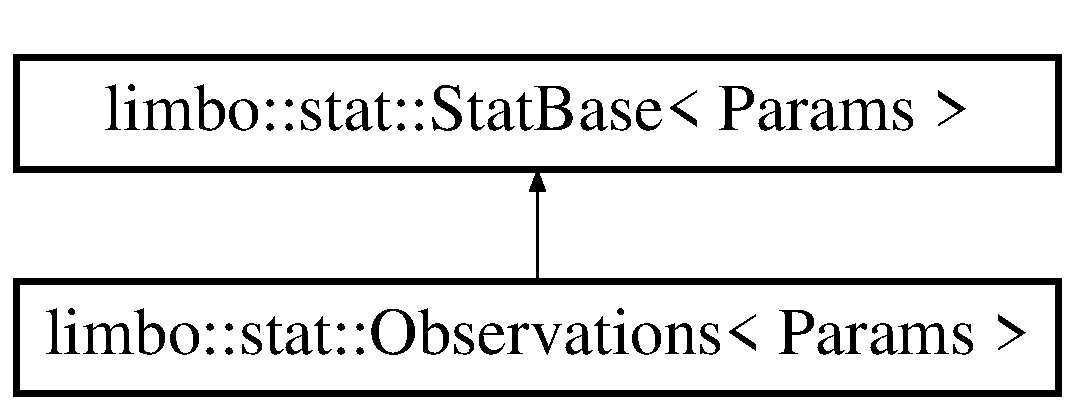
\includegraphics[height=2.000000cm]{structlimbo_1_1stat_1_1_observations}
\end{center}
\end{figure}
\subsection*{Public Member Functions}
\begin{DoxyCompactItemize}
\item 
{\footnotesize template$<$typename B\+O , typename Aggregator\+Function $>$ }\\void \hyperlink{structlimbo_1_1stat_1_1_observations_a7da8caabd4bc846a6bc17c08b8b1e5ad}{operator()} (const B\+O \&bo, const Aggregator\+Function \&, bool blacklisted)
\end{DoxyCompactItemize}


\subsection{Detailed Description}
\subsubsection*{template$<$typename Params$>$struct limbo\+::stat\+::\+Observations$<$ Params $>$}

filename\+: {\ttfamily observations.\+dat} 

\subsection{Member Function Documentation}
\hypertarget{structlimbo_1_1stat_1_1_observations_a7da8caabd4bc846a6bc17c08b8b1e5ad}{}\index{limbo\+::stat\+::\+Observations@{limbo\+::stat\+::\+Observations}!operator()@{operator()}}
\index{operator()@{operator()}!limbo\+::stat\+::\+Observations@{limbo\+::stat\+::\+Observations}}
\subsubsection[{operator()}]{\setlength{\rightskip}{0pt plus 5cm}template$<$typename Params $>$ template$<$typename B\+O , typename Aggregator\+Function $>$ void {\bf limbo\+::stat\+::\+Observations}$<$ Params $>$\+::operator() (
\begin{DoxyParamCaption}
\item[{const B\+O \&}]{bo, }
\item[{const Aggregator\+Function \&}]{, }
\item[{bool}]{blacklisted}
\end{DoxyParamCaption}
)\hspace{0.3cm}{\ttfamily [inline]}}\label{structlimbo_1_1stat_1_1_observations_a7da8caabd4bc846a6bc17c08b8b1e5ad}


The documentation for this struct was generated from the following file\+:\begin{DoxyCompactItemize}
\item 
/tmp/doc\+\_\+limbo/limbo/src/limbo/stat/\hyperlink{observations_8hpp}{observations.\+hpp}\end{DoxyCompactItemize}

\hypertarget{structlimbo_1_1defaults_1_1opt__cmaes}{}\section{limbo\+:\+:defaults\+:\+:opt\+\_\+cmaes Struct Reference}
\label{structlimbo_1_1defaults_1_1opt__cmaes}\index{limbo\+::defaults\+::opt\+\_\+cmaes@{limbo\+::defaults\+::opt\+\_\+cmaes}}


{\ttfamily \#include $<$limbo/opt/cmaes.\+hpp$>$}

\subsection*{Public Member Functions}
\begin{DoxyCompactItemize}
\item 
\hyperlink{group__opt__defaults_gaba7127b5e591a72095bd6c3a4155828d}{B\+O\+\_\+\+P\+A\+R\+A\+M} (int, restarts, 1)
\item 
\hyperlink{group__opt__defaults_ga5130bd236acff913c59380059474ebab}{B\+O\+\_\+\+P\+A\+R\+A\+M} (double, max\+\_\+fun\+\_\+evals,-\/1)
\item 
\hyperlink{group__opt__defaults_ga5f980ba02cafe6ee52d6b9cd485e3d05}{B\+O\+\_\+\+P\+A\+R\+A\+M} (double, fun\+\_\+tolerance,-\/1)
\item 
\hyperlink{group__opt__defaults_ga1b4276da9161bb04b84b4cd9307a37ab}{B\+O\+\_\+\+P\+A\+R\+A\+M} (double, fun\+\_\+target,-\/1)
\item 
\hyperlink{group__opt__defaults_ga14aff955e1360233e5ac361bdd2f3118}{B\+O\+\_\+\+P\+A\+R\+A\+M} (bool, fun\+\_\+compute\+\_\+initial, false)
\item 
\hyperlink{group__opt__defaults_gaf6fe5f409527ed056cee8cf8df52da9e}{B\+O\+\_\+\+P\+A\+R\+A\+M} (int, variant, a\+I\+P\+O\+P\+\_\+\+C\+M\+A\+E\+S)
\item 
\hyperlink{group__opt__defaults_ga660850db2d1f35863416f9790fe5125e}{B\+O\+\_\+\+P\+A\+R\+A\+M} (int, elitism, 0)
\item 
\hyperlink{group__opt__defaults_gad4f97065dd716df6c84e093059ab39f6}{B\+O\+\_\+\+P\+A\+R\+A\+M} (bool, handle\+\_\+uncertainty, false)
\item 
\hyperlink{group__opt__defaults_gae78e735b53742e438847fb63817f2ed1}{B\+O\+\_\+\+P\+A\+R\+A\+M} (bool, verbose, false)
\item 
\hyperlink{group__opt__defaults_ga0af64a0a2ea5ba01473e0cf284154dea}{B\+O\+\_\+\+P\+A\+R\+A\+M} (double, lbound, 0.\+0)
\item 
\hyperlink{group__opt__defaults_ga4d61ad0b07412ab14a72c008a8f99455}{B\+O\+\_\+\+P\+A\+R\+A\+M} (double, ubound, 1.\+0)
\end{DoxyCompactItemize}


The documentation for this struct was generated from the following file\+:\begin{DoxyCompactItemize}
\item 
/tmp/doc\+\_\+limbo/limbo/src/limbo/opt/\hyperlink{cmaes_8hpp}{cmaes.\+hpp}\end{DoxyCompactItemize}

\hypertarget{structlimbo_1_1defaults_1_1opt__gridsearch}{}\section{limbo\+:\+:defaults\+:\+:opt\+\_\+gridsearch Struct Reference}
\label{structlimbo_1_1defaults_1_1opt__gridsearch}\index{limbo\+::defaults\+::opt\+\_\+gridsearch@{limbo\+::defaults\+::opt\+\_\+gridsearch}}


{\ttfamily \#include $<$limbo/opt/grid\+\_\+search.\+hpp$>$}

\subsection*{Public Member Functions}
\begin{DoxyCompactItemize}
\item 
\hyperlink{group__opt__defaults_ga0ce56e9b25771d8a1b381b6ec132b8fe}{B\+O\+\_\+\+P\+A\+R\+AM} (int, bins, 5)
\end{DoxyCompactItemize}


The documentation for this struct was generated from the following file\+:\begin{DoxyCompactItemize}
\item 
/tmp/doc\+\_\+limbo/limbo/src/limbo/opt/\hyperlink{grid__search_8hpp}{grid\+\_\+search.\+hpp}\end{DoxyCompactItemize}

\hypertarget{structlimbo_1_1defaults_1_1opt__nloptgrad}{}\section{limbo\+:\+:defaults\+:\+:opt\+\_\+nloptgrad Struct Reference}
\label{structlimbo_1_1defaults_1_1opt__nloptgrad}\index{limbo\+::defaults\+::opt\+\_\+nloptgrad@{limbo\+::defaults\+::opt\+\_\+nloptgrad}}


{\ttfamily \#include $<$limbo/opt/nlopt\+\_\+grad.\+hpp$>$}

\subsection*{Public Member Functions}
\begin{DoxyCompactItemize}
\item 
\hyperlink{group__opt__defaults_ga4b0e251e3b7440148225201bcfc61f26}{B\+O\+\_\+\+P\+A\+R\+A\+M} (int, iterations, 500)
\end{DoxyCompactItemize}


The documentation for this struct was generated from the following file\+:\begin{DoxyCompactItemize}
\item 
/tmp/doc\+\_\+limbo/limbo/src/limbo/opt/\hyperlink{nlopt__grad_8hpp}{nlopt\+\_\+grad.\+hpp}\end{DoxyCompactItemize}

\hypertarget{structlimbo_1_1defaults_1_1opt__nloptnograd}{}\section{limbo\+:\+:defaults\+:\+:opt\+\_\+nloptnograd Struct Reference}
\label{structlimbo_1_1defaults_1_1opt__nloptnograd}\index{limbo\+::defaults\+::opt\+\_\+nloptnograd@{limbo\+::defaults\+::opt\+\_\+nloptnograd}}


{\ttfamily \#include $<$limbo/opt/nlopt\+\_\+no\+\_\+grad.\+hpp$>$}

\subsection*{Public Member Functions}
\begin{DoxyCompactItemize}
\item 
\hyperlink{group__opt__defaults_gae76755c949c322e0a8a33806c811b6f2}{B\+O\+\_\+\+P\+A\+R\+A\+M} (int, iterations, 500)
\end{DoxyCompactItemize}


The documentation for this struct was generated from the following file\+:\begin{DoxyCompactItemize}
\item 
/tmp/doc\+\_\+limbo/limbo/src/limbo/opt/\hyperlink{nlopt__no__grad_8hpp}{nlopt\+\_\+no\+\_\+grad.\+hpp}\end{DoxyCompactItemize}

\hypertarget{structlimbo_1_1defaults_1_1opt__parallelrepeater}{}\section{limbo\+:\+:defaults\+:\+:opt\+\_\+parallelrepeater Struct Reference}
\label{structlimbo_1_1defaults_1_1opt__parallelrepeater}\index{limbo\+::defaults\+::opt\+\_\+parallelrepeater@{limbo\+::defaults\+::opt\+\_\+parallelrepeater}}


{\ttfamily \#include $<$limbo/opt/parallel\+\_\+repeater.\+hpp$>$}

\subsection*{Public Member Functions}
\begin{DoxyCompactItemize}
\item 
\hyperlink{group__opt__defaults_ga4dfaebabf04a129cbb565807ed31f2de}{B\+O\+\_\+\+P\+A\+R\+A\+M} (int, repeats, 10)
\end{DoxyCompactItemize}


The documentation for this struct was generated from the following file\+:\begin{DoxyCompactItemize}
\item 
/tmp/doc\+\_\+limbo/limbo/src/limbo/opt/\hyperlink{parallel__repeater_8hpp}{parallel\+\_\+repeater.\+hpp}\end{DoxyCompactItemize}

\hypertarget{structlimbo_1_1defaults_1_1opt__rprop}{}\section{limbo\+:\+:defaults\+:\+:opt\+\_\+rprop Struct Reference}
\label{structlimbo_1_1defaults_1_1opt__rprop}\index{limbo\+::defaults\+::opt\+\_\+rprop@{limbo\+::defaults\+::opt\+\_\+rprop}}


{\ttfamily \#include $<$limbo/opt/rprop.\+hpp$>$}

\subsection*{Public Member Functions}
\begin{DoxyCompactItemize}
\item 
\hyperlink{group__opt__defaults_gadf6a8058cda20130ad992631e561eb5a}{B\+O\+\_\+\+P\+A\+R\+A\+M} (int, iterations, 300)
\end{DoxyCompactItemize}


The documentation for this struct was generated from the following file\+:\begin{DoxyCompactItemize}
\item 
/tmp/doc\+\_\+limbo/limbo/src/limbo/opt/\hyperlink{rprop_8hpp}{rprop.\+hpp}\end{DoxyCompactItemize}

\hypertarget{structlimbo_1_1opt_1_1_parallel_repeater}{}\section{limbo\+:\+:opt\+:\+:Parallel\+Repeater$<$ Params, Optimizer $>$ Struct Template Reference}
\label{structlimbo_1_1opt_1_1_parallel_repeater}\index{limbo\+::opt\+::\+Parallel\+Repeater$<$ Params, Optimizer $>$@{limbo\+::opt\+::\+Parallel\+Repeater$<$ Params, Optimizer $>$}}


{\ttfamily \#include $<$limbo/opt/parallel\+\_\+repeater.\+hpp$>$}

\subsection*{Public Member Functions}
\begin{DoxyCompactItemize}
\item 
{\footnotesize template$<$typename F $>$ }\\Eigen\+::\+Vector\+Xd \hyperlink{structlimbo_1_1opt_1_1_parallel_repeater_ac50bb2fc1525495c2025f0ff1c0cb021}{operator()} (const F \&f, const Eigen\+::\+Vector\+Xd \&init, bool bounded) const 
\end{DoxyCompactItemize}


\subsection{Detailed Description}
\subsubsection*{template$<$typename Params, typename Optimizer$>$struct limbo\+::opt\+::\+Parallel\+Repeater$<$ Params, Optimizer $>$}

Meta-\/optimizer\+: run the same algorithm in parallel many times from different init points and return the maximum found among all the replicates (useful for local algorithms)

Parameters\+:
\begin{DoxyItemize}
\item int repeats 
\end{DoxyItemize}

\subsection{Member Function Documentation}
\hypertarget{structlimbo_1_1opt_1_1_parallel_repeater_ac50bb2fc1525495c2025f0ff1c0cb021}{}\index{limbo\+::opt\+::\+Parallel\+Repeater@{limbo\+::opt\+::\+Parallel\+Repeater}!operator()@{operator()}}
\index{operator()@{operator()}!limbo\+::opt\+::\+Parallel\+Repeater@{limbo\+::opt\+::\+Parallel\+Repeater}}
\subsubsection[{operator()}]{\setlength{\rightskip}{0pt plus 5cm}template$<$typename Params , typename Optimizer $>$ template$<$typename F $>$ Eigen\+::\+Vector\+Xd {\bf limbo\+::opt\+::\+Parallel\+Repeater}$<$ Params, Optimizer $>$\+::operator() (
\begin{DoxyParamCaption}
\item[{const F \&}]{f, }
\item[{const Eigen\+::\+Vector\+Xd \&}]{init, }
\item[{bool}]{bounded}
\end{DoxyParamCaption}
) const\hspace{0.3cm}{\ttfamily [inline]}}\label{structlimbo_1_1opt_1_1_parallel_repeater_ac50bb2fc1525495c2025f0ff1c0cb021}


The documentation for this struct was generated from the following file\+:\begin{DoxyCompactItemize}
\item 
/tmp/doc\+\_\+limbo/limbo/src/limbo/opt/\hyperlink{parallel__repeater_8hpp}{parallel\+\_\+repeater.\+hpp}\end{DoxyCompactItemize}

\hypertarget{classlimbo_1_1experimental_1_1bayes__opt_1_1_parego}{}\section{limbo\+:\+:experimental\+:\+:bayes\+\_\+opt\+:\+:Parego$<$ Params, A1, A2, A3, A4, A5 $>$ Class Template Reference}
\label{classlimbo_1_1experimental_1_1bayes__opt_1_1_parego}\index{limbo\+::experimental\+::bayes\+\_\+opt\+::\+Parego$<$ Params, A1, A2, A3, A4, A5 $>$@{limbo\+::experimental\+::bayes\+\_\+opt\+::\+Parego$<$ Params, A1, A2, A3, A4, A5 $>$}}


{\ttfamily \#include $<$limbo/experimental/bayes\+\_\+opt/parego.\+hpp$>$}

Inheritance diagram for limbo\+:\+:experimental\+:\+:bayes\+\_\+opt\+:\+:Parego$<$ Params, A1, A2, A3, A4, A5 $>$\+:\begin{figure}[H]
\begin{center}
\leavevmode
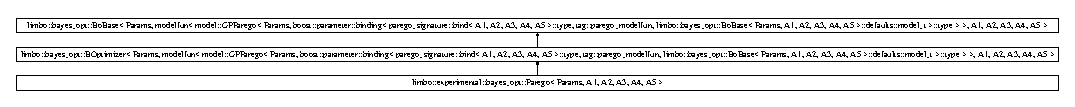
\includegraphics[height=0.993495cm]{classlimbo_1_1experimental_1_1bayes__opt_1_1_parego}
\end{center}
\end{figure}
\subsection*{Additional Inherited Members}


The documentation for this class was generated from the following file\+:\begin{DoxyCompactItemize}
\item 
/tmp/doc\+\_\+limbo/limbo/src/limbo/experimental/bayes\+\_\+opt/\hyperlink{parego_8hpp}{parego.\+hpp}\end{DoxyCompactItemize}

\hypertarget{structlimbo_1_1experimental_1_1stat_1_1_pareto_benchmark}{}\section{limbo\+:\+:experimental\+:\+:stat\+:\+:Pareto\+Benchmark$<$ F $>$ Struct Template Reference}
\label{structlimbo_1_1experimental_1_1stat_1_1_pareto_benchmark}\index{limbo\+::experimental\+::stat\+::\+Pareto\+Benchmark$<$ F $>$@{limbo\+::experimental\+::stat\+::\+Pareto\+Benchmark$<$ F $>$}}


{\ttfamily \#include $<$limbo/experimental/stat/pareto\+\_\+benchmark.\+hpp$>$}

\subsection*{Public Member Functions}
\begin{DoxyCompactItemize}
\item 
{\footnotesize template$<$typename B\+O , typename Aggregator\+Function $>$ }\\void \hyperlink{structlimbo_1_1experimental_1_1stat_1_1_pareto_benchmark_a27b8cf1f9dcda186631fb0f37528028f}{operator()} (B\+O \&opt, const Aggregator\+Function \&afun, bool blacklisted)
\end{DoxyCompactItemize}


\subsection{Member Function Documentation}
\hypertarget{structlimbo_1_1experimental_1_1stat_1_1_pareto_benchmark_a27b8cf1f9dcda186631fb0f37528028f}{}\index{limbo\+::experimental\+::stat\+::\+Pareto\+Benchmark@{limbo\+::experimental\+::stat\+::\+Pareto\+Benchmark}!operator()@{operator()}}
\index{operator()@{operator()}!limbo\+::experimental\+::stat\+::\+Pareto\+Benchmark@{limbo\+::experimental\+::stat\+::\+Pareto\+Benchmark}}
\subsubsection[{operator()}]{\setlength{\rightskip}{0pt plus 5cm}template$<$typename F $>$ template$<$typename B\+O , typename Aggregator\+Function $>$ void {\bf limbo\+::experimental\+::stat\+::\+Pareto\+Benchmark}$<$ F $>$\+::operator() (
\begin{DoxyParamCaption}
\item[{B\+O \&}]{opt, }
\item[{const Aggregator\+Function \&}]{afun, }
\item[{bool}]{blacklisted}
\end{DoxyParamCaption}
)\hspace{0.3cm}{\ttfamily [inline]}}\label{structlimbo_1_1experimental_1_1stat_1_1_pareto_benchmark_a27b8cf1f9dcda186631fb0f37528028f}


The documentation for this struct was generated from the following file\+:\begin{DoxyCompactItemize}
\item 
/tmp/doc\+\_\+limbo/limbo/src/limbo/experimental/stat/\hyperlink{pareto__benchmark_8hpp}{pareto\+\_\+benchmark.\+hpp}\end{DoxyCompactItemize}

\hypertarget{structlimbo_1_1experimental_1_1stat_1_1_pareto_front}{}\section{limbo\+:\+:experimental\+:\+:stat\+:\+:Pareto\+Front$<$ Params $>$ Struct Template Reference}
\label{structlimbo_1_1experimental_1_1stat_1_1_pareto_front}\index{limbo\+::experimental\+::stat\+::\+Pareto\+Front$<$ Params $>$@{limbo\+::experimental\+::stat\+::\+Pareto\+Front$<$ Params $>$}}


{\ttfamily \#include $<$limbo/experimental/stat/pareto\+\_\+front.\+hpp$>$}

Inheritance diagram for limbo\+:\+:experimental\+:\+:stat\+:\+:Pareto\+Front$<$ Params $>$\+:\begin{figure}[H]
\begin{center}
\leavevmode
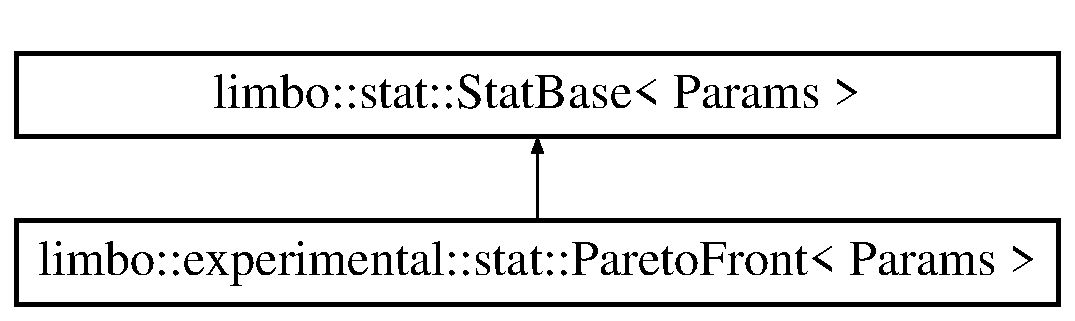
\includegraphics[height=2.000000cm]{structlimbo_1_1experimental_1_1stat_1_1_pareto_front}
\end{center}
\end{figure}
\subsection*{Public Types}
\begin{DoxyCompactItemize}
\item 
using \hyperlink{structlimbo_1_1experimental_1_1stat_1_1_pareto_front_a2d872d2ad0a93b4c459bad640be158b9}{pareto\+\_\+point\+\_\+t} = std\+::tuple$<$ Eigen\+::\+Vector\+Xd, Eigen\+::\+Vector\+Xd, Eigen\+::\+Vector\+Xd $>$
\item 
using \hyperlink{structlimbo_1_1experimental_1_1stat_1_1_pareto_front_a710260d53bff65b4841c348b074a6e23}{pareto\+\_\+t} = std\+::vector$<$ \hyperlink{structlimbo_1_1experimental_1_1stat_1_1_pareto_front_a2d872d2ad0a93b4c459bad640be158b9}{pareto\+\_\+point\+\_\+t} $>$
\end{DoxyCompactItemize}
\subsection*{Public Member Functions}
\begin{DoxyCompactItemize}
\item 
{\footnotesize template$<$typename BO , typename Aggregator\+Function $>$ }\\void \hyperlink{structlimbo_1_1experimental_1_1stat_1_1_pareto_front_a341b34d96290a874818bbdb4f27f9f2b}{operator()} (const BO \&bo, const Aggregator\+Function \&)
\end{DoxyCompactItemize}


\subsection{Member Typedef Documentation}
\index{limbo\+::experimental\+::stat\+::\+Pareto\+Front@{limbo\+::experimental\+::stat\+::\+Pareto\+Front}!pareto\+\_\+point\+\_\+t@{pareto\+\_\+point\+\_\+t}}
\index{pareto\+\_\+point\+\_\+t@{pareto\+\_\+point\+\_\+t}!limbo\+::experimental\+::stat\+::\+Pareto\+Front@{limbo\+::experimental\+::stat\+::\+Pareto\+Front}}
\subsubsection[{\texorpdfstring{pareto\+\_\+point\+\_\+t}{pareto_point_t}}]{\setlength{\rightskip}{0pt plus 5cm}template$<$typename Params $>$ using {\bf limbo\+::experimental\+::stat\+::\+Pareto\+Front}$<$ Params $>$\+::{\bf pareto\+\_\+point\+\_\+t} =  std\+::tuple$<$Eigen\+::\+Vector\+Xd, Eigen\+::\+Vector\+Xd, Eigen\+::\+Vector\+Xd$>$}\hypertarget{structlimbo_1_1experimental_1_1stat_1_1_pareto_front_a2d872d2ad0a93b4c459bad640be158b9}{}\label{structlimbo_1_1experimental_1_1stat_1_1_pareto_front_a2d872d2ad0a93b4c459bad640be158b9}
\index{limbo\+::experimental\+::stat\+::\+Pareto\+Front@{limbo\+::experimental\+::stat\+::\+Pareto\+Front}!pareto\+\_\+t@{pareto\+\_\+t}}
\index{pareto\+\_\+t@{pareto\+\_\+t}!limbo\+::experimental\+::stat\+::\+Pareto\+Front@{limbo\+::experimental\+::stat\+::\+Pareto\+Front}}
\subsubsection[{\texorpdfstring{pareto\+\_\+t}{pareto_t}}]{\setlength{\rightskip}{0pt plus 5cm}template$<$typename Params $>$ using {\bf limbo\+::experimental\+::stat\+::\+Pareto\+Front}$<$ Params $>$\+::{\bf pareto\+\_\+t} =  std\+::vector$<${\bf pareto\+\_\+point\+\_\+t}$>$}\hypertarget{structlimbo_1_1experimental_1_1stat_1_1_pareto_front_a710260d53bff65b4841c348b074a6e23}{}\label{structlimbo_1_1experimental_1_1stat_1_1_pareto_front_a710260d53bff65b4841c348b074a6e23}


\subsection{Member Function Documentation}
\index{limbo\+::experimental\+::stat\+::\+Pareto\+Front@{limbo\+::experimental\+::stat\+::\+Pareto\+Front}!operator()@{operator()}}
\index{operator()@{operator()}!limbo\+::experimental\+::stat\+::\+Pareto\+Front@{limbo\+::experimental\+::stat\+::\+Pareto\+Front}}
\subsubsection[{\texorpdfstring{operator()(const B\+O \&bo, const Aggregator\+Function \&)}{operator()(const BO &bo, const AggregatorFunction &)}}]{\setlength{\rightskip}{0pt plus 5cm}template$<$typename Params $>$ template$<$typename BO , typename Aggregator\+Function $>$ void {\bf limbo\+::experimental\+::stat\+::\+Pareto\+Front}$<$ Params $>$\+::operator() (
\begin{DoxyParamCaption}
\item[{const BO \&}]{bo, }
\item[{const Aggregator\+Function \&}]{}
\end{DoxyParamCaption}
)\hspace{0.3cm}{\ttfamily [inline]}}\hypertarget{structlimbo_1_1experimental_1_1stat_1_1_pareto_front_a341b34d96290a874818bbdb4f27f9f2b}{}\label{structlimbo_1_1experimental_1_1stat_1_1_pareto_front_a341b34d96290a874818bbdb4f27f9f2b}


The documentation for this struct was generated from the following file\+:\begin{DoxyCompactItemize}
\item 
/tmp/doc\+\_\+limbo/limbo/src/limbo/experimental/stat/\hyperlink{pareto__front_8hpp}{pareto\+\_\+front.\+hpp}\end{DoxyCompactItemize}

\hypertarget{classrandutils_1_1random__generator}{}\section{randutils\+:\+:random\+\_\+generator$<$ Random\+Engine, Default\+Seed\+Seq $>$ Class Template Reference}
\label{classrandutils_1_1random__generator}\index{randutils\+::random\+\_\+generator$<$ Random\+Engine, Default\+Seed\+Seq $>$@{randutils\+::random\+\_\+generator$<$ Random\+Engine, Default\+Seed\+Seq $>$}}


{\ttfamily \#include $<$limbo/tools/rand\+\_\+utils.\+hpp$>$}

\subsection*{Public Types}
\begin{DoxyCompactItemize}
\item 
using \hyperlink{classrandutils_1_1random__generator_a7ccbb95be67d7cd19f4b128be21b4ac3}{engine\+\_\+type} = Random\+Engine
\item 
using \hyperlink{classrandutils_1_1random__generator_a424b01b5232f91d42163369ad6bd3b11}{default\+\_\+seed\+\_\+type} = Default\+Seed\+Seq
\end{DoxyCompactItemize}
\subsection*{Public Member Functions}
\begin{DoxyCompactItemize}
\item 
{\footnotesize template$<$typename Seeding  = default\+\_\+seed\+\_\+type, typename... Params$>$ }\\\hyperlink{classrandutils_1_1random__generator_abfccab3973766dbd0526bc8269f26cff}{random\+\_\+generator} (Seeding \&\&seeding=\hyperlink{classrandutils_1_1random__generator_a424b01b5232f91d42163369ad6bd3b11}{default\+\_\+seed\+\_\+type}\{\})
\item 
{\footnotesize template$<$typename Seeding , typename... Params$>$ }\\\hyperlink{classrandutils_1_1random__generator_ab706901b79a9fceb71e3ad7fd7031ae4}{random\+\_\+generator} (Seeding \&\&seeding, Params \&\&...params)
\item 
{\footnotesize template$<$typename Seeding  = default\+\_\+seed\+\_\+type, typename... Params$>$ }\\void \hyperlink{classrandutils_1_1random__generator_ae25cea4c3bd86714fb8f2c2135842e68}{seed} (Seeding \&\&seeding=\hyperlink{classrandutils_1_1random__generator_a424b01b5232f91d42163369ad6bd3b11}{default\+\_\+seed\+\_\+type}\{\})
\item 
{\footnotesize template$<$typename Seeding , typename... Params$>$ }\\void \hyperlink{classrandutils_1_1random__generator_a05fa4e4dba44982912c32562dc8e16d8}{seed} (Seeding \&\&seeding, Params \&\&...params)
\item 
Random\+Engine \& \hyperlink{classrandutils_1_1random__generator_a85303ed792296a49a8f395fb3a71c2ed}{engine} ()
\item 
{\footnotesize template$<$typename Result\+Type , template$<$ typename $>$ class Dist\+Tmpl = std\+::normal\+\_\+distribution, typename... Params$>$ }\\Result\+Type \hyperlink{classrandutils_1_1random__generator_a4aed9ef9fe1695d08b9b30891f1127b3}{variate} (Params \&\&...params)
\item 
{\footnotesize template$<$typename Numeric $>$ }\\Numeric \hyperlink{classrandutils_1_1random__generator_a122935c5a83df7f584d7120c64c732bc}{uniform} (Numeric lower, Numeric upper)
\item 
{\footnotesize template$<$template$<$ typename $>$ class Dist\+Tmpl = uniform\+\_\+distribution, typename Iter , typename... Params$>$ }\\void \hyperlink{classrandutils_1_1random__generator_aa0e413e887ea03dfd1653d0b071f70bf}{generate} (Iter first, Iter last, Params \&\&...params)
\item 
{\footnotesize template$<$template$<$ typename $>$ class Dist\+Tmpl = uniform\+\_\+distribution, typename Range , typename... Params$>$ }\\void \hyperlink{classrandutils_1_1random__generator_ae061f844df411efc2ebfe6c3bbc6f206}{generate} (Range \&\&range, Params \&\&...params)
\item 
{\footnotesize template$<$typename Iter $>$ }\\void \hyperlink{classrandutils_1_1random__generator_aaa2790b3799d1a62d489ae3efefbb006}{shuffle} (Iter first, Iter last)
\item 
{\footnotesize template$<$typename Range $>$ }\\void \hyperlink{classrandutils_1_1random__generator_a96bd60aadafa23dc853dcd9414f26b69}{shuffle} (Range \&\&range)
\item 
{\footnotesize template$<$typename Iter $>$ }\\Iter \hyperlink{classrandutils_1_1random__generator_a29f305cbca6d418d4c2ddbf60953dc42}{choose} (Iter first, Iter last)
\item 
{\footnotesize template$<$typename Range $>$ }\\auto \hyperlink{classrandutils_1_1random__generator_a0eafdcc64b6d0967d9668a0775628af6}{choose} (Range \&\&range) -\/$>$ decltype(std\+::begin(range))
\item 
{\footnotesize template$<$typename Range $>$ }\\auto \hyperlink{classrandutils_1_1random__generator_a6d9a9002b313cf8126bf640f728f3c49}{pick} (Range \&\&range) -\/$>$ decltype($\ast$std\+::begin(range))
\item 
{\footnotesize template$<$typename T $>$ }\\auto \hyperlink{classrandutils_1_1random__generator_aab0a1c9def1a609d5739eddf5ca8caeb}{pick} (std\+::initializer\+\_\+list$<$ T $>$ range) -\/$>$ decltype($\ast$range.\+begin())
\item 
{\footnotesize template$<$typename Size , typename Iter $>$ }\\Iter \hyperlink{classrandutils_1_1random__generator_a6572f276cd3c8fd547ffbefce5cd4dc4}{sample} (Size to\+\_\+go, Iter first, Iter last)
\item 
{\footnotesize template$<$typename Size , typename Range $>$ }\\auto \hyperlink{classrandutils_1_1random__generator_a1f99da2d77fccea01edc3a5fe32255ac}{sample} (Size to\+\_\+go, Range \&\&range) -\/$>$ decltype(std\+::begin(range))
\end{DoxyCompactItemize}


\subsection{Member Typedef Documentation}
\index{randutils\+::random\+\_\+generator@{randutils\+::random\+\_\+generator}!default\+\_\+seed\+\_\+type@{default\+\_\+seed\+\_\+type}}
\index{default\+\_\+seed\+\_\+type@{default\+\_\+seed\+\_\+type}!randutils\+::random\+\_\+generator@{randutils\+::random\+\_\+generator}}
\subsubsection[{\texorpdfstring{default\+\_\+seed\+\_\+type}{default_seed_type}}]{\setlength{\rightskip}{0pt plus 5cm}template$<$typename Random\+Engine  = std\+::default\+\_\+random\+\_\+engine, typename Default\+Seed\+Seq  = auto\+\_\+seed\+\_\+256$>$ using {\bf randutils\+::random\+\_\+generator}$<$ Random\+Engine, Default\+Seed\+Seq $>$\+::{\bf default\+\_\+seed\+\_\+type} =  Default\+Seed\+Seq}\hypertarget{classrandutils_1_1random__generator_a424b01b5232f91d42163369ad6bd3b11}{}\label{classrandutils_1_1random__generator_a424b01b5232f91d42163369ad6bd3b11}
\index{randutils\+::random\+\_\+generator@{randutils\+::random\+\_\+generator}!engine\+\_\+type@{engine\+\_\+type}}
\index{engine\+\_\+type@{engine\+\_\+type}!randutils\+::random\+\_\+generator@{randutils\+::random\+\_\+generator}}
\subsubsection[{\texorpdfstring{engine\+\_\+type}{engine_type}}]{\setlength{\rightskip}{0pt plus 5cm}template$<$typename Random\+Engine  = std\+::default\+\_\+random\+\_\+engine, typename Default\+Seed\+Seq  = auto\+\_\+seed\+\_\+256$>$ using {\bf randutils\+::random\+\_\+generator}$<$ Random\+Engine, Default\+Seed\+Seq $>$\+::{\bf engine\+\_\+type} =  Random\+Engine}\hypertarget{classrandutils_1_1random__generator_a7ccbb95be67d7cd19f4b128be21b4ac3}{}\label{classrandutils_1_1random__generator_a7ccbb95be67d7cd19f4b128be21b4ac3}


\subsection{Constructor \& Destructor Documentation}
\index{randutils\+::random\+\_\+generator@{randutils\+::random\+\_\+generator}!random\+\_\+generator@{random\+\_\+generator}}
\index{random\+\_\+generator@{random\+\_\+generator}!randutils\+::random\+\_\+generator@{randutils\+::random\+\_\+generator}}
\subsubsection[{\texorpdfstring{random\+\_\+generator(\+Seeding \&\&seeding=default\+\_\+seed\+\_\+type\lcurly{}\rcurly{})}{random_generator(Seeding &&seeding=default_seed_type\{\})}}]{\setlength{\rightskip}{0pt plus 5cm}template$<$typename Random\+Engine  = std\+::default\+\_\+random\+\_\+engine, typename Default\+Seed\+Seq  = auto\+\_\+seed\+\_\+256$>$ template$<$typename Seeding  = default\+\_\+seed\+\_\+type, typename... Params$>$ {\bf randutils\+::random\+\_\+generator}$<$ Random\+Engine, Default\+Seed\+Seq $>$\+::{\bf random\+\_\+generator} (
\begin{DoxyParamCaption}
\item[{Seeding \&\&}]{seeding = {\ttfamily {\bf default\+\_\+seed\+\_\+type}\{\}}}
\end{DoxyParamCaption}
)\hspace{0.3cm}{\ttfamily [inline]}}\hypertarget{classrandutils_1_1random__generator_abfccab3973766dbd0526bc8269f26cff}{}\label{classrandutils_1_1random__generator_abfccab3973766dbd0526bc8269f26cff}
\index{randutils\+::random\+\_\+generator@{randutils\+::random\+\_\+generator}!random\+\_\+generator@{random\+\_\+generator}}
\index{random\+\_\+generator@{random\+\_\+generator}!randutils\+::random\+\_\+generator@{randutils\+::random\+\_\+generator}}
\subsubsection[{\texorpdfstring{random\+\_\+generator(\+Seeding \&\&seeding, Params \&\&...\+params)}{random_generator(Seeding &&seeding, Params &&...params)}}]{\setlength{\rightskip}{0pt plus 5cm}template$<$typename Random\+Engine  = std\+::default\+\_\+random\+\_\+engine, typename Default\+Seed\+Seq  = auto\+\_\+seed\+\_\+256$>$ template$<$typename Seeding , typename... Params$>$ {\bf randutils\+::random\+\_\+generator}$<$ Random\+Engine, Default\+Seed\+Seq $>$\+::{\bf random\+\_\+generator} (
\begin{DoxyParamCaption}
\item[{Seeding \&\&}]{seeding, }
\item[{Params \&\&...}]{params}
\end{DoxyParamCaption}
)\hspace{0.3cm}{\ttfamily [inline]}}\hypertarget{classrandutils_1_1random__generator_ab706901b79a9fceb71e3ad7fd7031ae4}{}\label{classrandutils_1_1random__generator_ab706901b79a9fceb71e3ad7fd7031ae4}


\subsection{Member Function Documentation}
\index{randutils\+::random\+\_\+generator@{randutils\+::random\+\_\+generator}!choose@{choose}}
\index{choose@{choose}!randutils\+::random\+\_\+generator@{randutils\+::random\+\_\+generator}}
\subsubsection[{\texorpdfstring{choose(\+Iter first, Iter last)}{choose(Iter first, Iter last)}}]{\setlength{\rightskip}{0pt plus 5cm}template$<$typename Random\+Engine  = std\+::default\+\_\+random\+\_\+engine, typename Default\+Seed\+Seq  = auto\+\_\+seed\+\_\+256$>$ template$<$typename Iter $>$ Iter {\bf randutils\+::random\+\_\+generator}$<$ Random\+Engine, Default\+Seed\+Seq $>$\+::choose (
\begin{DoxyParamCaption}
\item[{Iter}]{first, }
\item[{Iter}]{last}
\end{DoxyParamCaption}
)\hspace{0.3cm}{\ttfamily [inline]}}\hypertarget{classrandutils_1_1random__generator_a29f305cbca6d418d4c2ddbf60953dc42}{}\label{classrandutils_1_1random__generator_a29f305cbca6d418d4c2ddbf60953dc42}
\index{randutils\+::random\+\_\+generator@{randutils\+::random\+\_\+generator}!choose@{choose}}
\index{choose@{choose}!randutils\+::random\+\_\+generator@{randutils\+::random\+\_\+generator}}
\subsubsection[{\texorpdfstring{choose(\+Range \&\&range) -\/$>$ decltype(std\+::begin(range))}{choose(Range &&range) -> decltype(std::begin(range))}}]{\setlength{\rightskip}{0pt plus 5cm}template$<$typename Random\+Engine  = std\+::default\+\_\+random\+\_\+engine, typename Default\+Seed\+Seq  = auto\+\_\+seed\+\_\+256$>$ template$<$typename Range $>$ auto {\bf randutils\+::random\+\_\+generator}$<$ Random\+Engine, Default\+Seed\+Seq $>$\+::choose (
\begin{DoxyParamCaption}
\item[{Range \&\&}]{range}
\end{DoxyParamCaption}
) -\/$>$ decltype(std\+::begin(range))
        \hspace{0.3cm}{\ttfamily [inline]}}\hypertarget{classrandutils_1_1random__generator_a0eafdcc64b6d0967d9668a0775628af6}{}\label{classrandutils_1_1random__generator_a0eafdcc64b6d0967d9668a0775628af6}
\index{randutils\+::random\+\_\+generator@{randutils\+::random\+\_\+generator}!engine@{engine}}
\index{engine@{engine}!randutils\+::random\+\_\+generator@{randutils\+::random\+\_\+generator}}
\subsubsection[{\texorpdfstring{engine()}{engine()}}]{\setlength{\rightskip}{0pt plus 5cm}template$<$typename Random\+Engine  = std\+::default\+\_\+random\+\_\+engine, typename Default\+Seed\+Seq  = auto\+\_\+seed\+\_\+256$>$ Random\+Engine\& {\bf randutils\+::random\+\_\+generator}$<$ Random\+Engine, Default\+Seed\+Seq $>$\+::engine (
\begin{DoxyParamCaption}
{}
\end{DoxyParamCaption}
)\hspace{0.3cm}{\ttfamily [inline]}}\hypertarget{classrandutils_1_1random__generator_a85303ed792296a49a8f395fb3a71c2ed}{}\label{classrandutils_1_1random__generator_a85303ed792296a49a8f395fb3a71c2ed}
\index{randutils\+::random\+\_\+generator@{randutils\+::random\+\_\+generator}!generate@{generate}}
\index{generate@{generate}!randutils\+::random\+\_\+generator@{randutils\+::random\+\_\+generator}}
\subsubsection[{\texorpdfstring{generate(\+Iter first, Iter last, Params \&\&...\+params)}{generate(Iter first, Iter last, Params &&...params)}}]{\setlength{\rightskip}{0pt plus 5cm}template$<$typename Random\+Engine  = std\+::default\+\_\+random\+\_\+engine, typename Default\+Seed\+Seq  = auto\+\_\+seed\+\_\+256$>$ template$<$template$<$ typename $>$ class Dist\+Tmpl = uniform\+\_\+distribution, typename Iter , typename... Params$>$ void {\bf randutils\+::random\+\_\+generator}$<$ Random\+Engine, Default\+Seed\+Seq $>$\+::generate (
\begin{DoxyParamCaption}
\item[{Iter}]{first, }
\item[{Iter}]{last, }
\item[{Params \&\&...}]{params}
\end{DoxyParamCaption}
)\hspace{0.3cm}{\ttfamily [inline]}}\hypertarget{classrandutils_1_1random__generator_aa0e413e887ea03dfd1653d0b071f70bf}{}\label{classrandutils_1_1random__generator_aa0e413e887ea03dfd1653d0b071f70bf}
\index{randutils\+::random\+\_\+generator@{randutils\+::random\+\_\+generator}!generate@{generate}}
\index{generate@{generate}!randutils\+::random\+\_\+generator@{randutils\+::random\+\_\+generator}}
\subsubsection[{\texorpdfstring{generate(\+Range \&\&range, Params \&\&...\+params)}{generate(Range &&range, Params &&...params)}}]{\setlength{\rightskip}{0pt plus 5cm}template$<$typename Random\+Engine  = std\+::default\+\_\+random\+\_\+engine, typename Default\+Seed\+Seq  = auto\+\_\+seed\+\_\+256$>$ template$<$template$<$ typename $>$ class Dist\+Tmpl = uniform\+\_\+distribution, typename Range , typename... Params$>$ void {\bf randutils\+::random\+\_\+generator}$<$ Random\+Engine, Default\+Seed\+Seq $>$\+::generate (
\begin{DoxyParamCaption}
\item[{Range \&\&}]{range, }
\item[{Params \&\&...}]{params}
\end{DoxyParamCaption}
)\hspace{0.3cm}{\ttfamily [inline]}}\hypertarget{classrandutils_1_1random__generator_ae061f844df411efc2ebfe6c3bbc6f206}{}\label{classrandutils_1_1random__generator_ae061f844df411efc2ebfe6c3bbc6f206}
\index{randutils\+::random\+\_\+generator@{randutils\+::random\+\_\+generator}!pick@{pick}}
\index{pick@{pick}!randutils\+::random\+\_\+generator@{randutils\+::random\+\_\+generator}}
\subsubsection[{\texorpdfstring{pick(\+Range \&\&range) -\/$>$ decltype($\ast$std\+::begin(range))}{pick(Range &&range) -> decltype(*std::begin(range))}}]{\setlength{\rightskip}{0pt plus 5cm}template$<$typename Random\+Engine  = std\+::default\+\_\+random\+\_\+engine, typename Default\+Seed\+Seq  = auto\+\_\+seed\+\_\+256$>$ template$<$typename Range $>$ auto {\bf randutils\+::random\+\_\+generator}$<$ Random\+Engine, Default\+Seed\+Seq $>$\+::pick (
\begin{DoxyParamCaption}
\item[{Range \&\&}]{range}
\end{DoxyParamCaption}
) -\/$>$ decltype($\ast$std\+::begin(range))
        \hspace{0.3cm}{\ttfamily [inline]}}\hypertarget{classrandutils_1_1random__generator_a6d9a9002b313cf8126bf640f728f3c49}{}\label{classrandutils_1_1random__generator_a6d9a9002b313cf8126bf640f728f3c49}
\index{randutils\+::random\+\_\+generator@{randutils\+::random\+\_\+generator}!pick@{pick}}
\index{pick@{pick}!randutils\+::random\+\_\+generator@{randutils\+::random\+\_\+generator}}
\subsubsection[{\texorpdfstring{pick(std\+::initializer\+\_\+list$<$ T $>$ range) -\/$>$ decltype($\ast$range.\+begin())}{pick(std::initializer_list< T > range) -> decltype(*range.begin())}}]{\setlength{\rightskip}{0pt plus 5cm}template$<$typename Random\+Engine  = std\+::default\+\_\+random\+\_\+engine, typename Default\+Seed\+Seq  = auto\+\_\+seed\+\_\+256$>$ template$<$typename T $>$ auto {\bf randutils\+::random\+\_\+generator}$<$ Random\+Engine, Default\+Seed\+Seq $>$\+::pick (
\begin{DoxyParamCaption}
\item[{std\+::initializer\+\_\+list$<$ T $>$}]{range}
\end{DoxyParamCaption}
) -\/$>$ decltype($\ast$range.\+begin())
        \hspace{0.3cm}{\ttfamily [inline]}}\hypertarget{classrandutils_1_1random__generator_aab0a1c9def1a609d5739eddf5ca8caeb}{}\label{classrandutils_1_1random__generator_aab0a1c9def1a609d5739eddf5ca8caeb}
\index{randutils\+::random\+\_\+generator@{randutils\+::random\+\_\+generator}!sample@{sample}}
\index{sample@{sample}!randutils\+::random\+\_\+generator@{randutils\+::random\+\_\+generator}}
\subsubsection[{\texorpdfstring{sample(\+Size to\+\_\+go, Iter first, Iter last)}{sample(Size to_go, Iter first, Iter last)}}]{\setlength{\rightskip}{0pt plus 5cm}template$<$typename Random\+Engine  = std\+::default\+\_\+random\+\_\+engine, typename Default\+Seed\+Seq  = auto\+\_\+seed\+\_\+256$>$ template$<$typename Size , typename Iter $>$ Iter {\bf randutils\+::random\+\_\+generator}$<$ Random\+Engine, Default\+Seed\+Seq $>$\+::sample (
\begin{DoxyParamCaption}
\item[{Size}]{to\+\_\+go, }
\item[{Iter}]{first, }
\item[{Iter}]{last}
\end{DoxyParamCaption}
)\hspace{0.3cm}{\ttfamily [inline]}}\hypertarget{classrandutils_1_1random__generator_a6572f276cd3c8fd547ffbefce5cd4dc4}{}\label{classrandutils_1_1random__generator_a6572f276cd3c8fd547ffbefce5cd4dc4}
\index{randutils\+::random\+\_\+generator@{randutils\+::random\+\_\+generator}!sample@{sample}}
\index{sample@{sample}!randutils\+::random\+\_\+generator@{randutils\+::random\+\_\+generator}}
\subsubsection[{\texorpdfstring{sample(\+Size to\+\_\+go, Range \&\&range) -\/$>$ decltype(std\+::begin(range))}{sample(Size to_go, Range &&range) -> decltype(std::begin(range))}}]{\setlength{\rightskip}{0pt plus 5cm}template$<$typename Random\+Engine  = std\+::default\+\_\+random\+\_\+engine, typename Default\+Seed\+Seq  = auto\+\_\+seed\+\_\+256$>$ template$<$typename Size , typename Range $>$ auto {\bf randutils\+::random\+\_\+generator}$<$ Random\+Engine, Default\+Seed\+Seq $>$\+::sample (
\begin{DoxyParamCaption}
\item[{Size}]{to\+\_\+go, }
\item[{Range \&\&}]{range}
\end{DoxyParamCaption}
) -\/$>$ decltype(std\+::begin(range))
        \hspace{0.3cm}{\ttfamily [inline]}}\hypertarget{classrandutils_1_1random__generator_a1f99da2d77fccea01edc3a5fe32255ac}{}\label{classrandutils_1_1random__generator_a1f99da2d77fccea01edc3a5fe32255ac}
\index{randutils\+::random\+\_\+generator@{randutils\+::random\+\_\+generator}!seed@{seed}}
\index{seed@{seed}!randutils\+::random\+\_\+generator@{randutils\+::random\+\_\+generator}}
\subsubsection[{\texorpdfstring{seed(\+Seeding \&\&seeding=default\+\_\+seed\+\_\+type\lcurly{}\rcurly{})}{seed(Seeding &&seeding=default_seed_type\{\})}}]{\setlength{\rightskip}{0pt plus 5cm}template$<$typename Random\+Engine  = std\+::default\+\_\+random\+\_\+engine, typename Default\+Seed\+Seq  = auto\+\_\+seed\+\_\+256$>$ template$<$typename Seeding  = default\+\_\+seed\+\_\+type, typename... Params$>$ void {\bf randutils\+::random\+\_\+generator}$<$ Random\+Engine, Default\+Seed\+Seq $>$\+::seed (
\begin{DoxyParamCaption}
\item[{Seeding \&\&}]{seeding = {\ttfamily {\bf default\+\_\+seed\+\_\+type}\{\}}}
\end{DoxyParamCaption}
)\hspace{0.3cm}{\ttfamily [inline]}}\hypertarget{classrandutils_1_1random__generator_ae25cea4c3bd86714fb8f2c2135842e68}{}\label{classrandutils_1_1random__generator_ae25cea4c3bd86714fb8f2c2135842e68}
\index{randutils\+::random\+\_\+generator@{randutils\+::random\+\_\+generator}!seed@{seed}}
\index{seed@{seed}!randutils\+::random\+\_\+generator@{randutils\+::random\+\_\+generator}}
\subsubsection[{\texorpdfstring{seed(\+Seeding \&\&seeding, Params \&\&...\+params)}{seed(Seeding &&seeding, Params &&...params)}}]{\setlength{\rightskip}{0pt plus 5cm}template$<$typename Random\+Engine  = std\+::default\+\_\+random\+\_\+engine, typename Default\+Seed\+Seq  = auto\+\_\+seed\+\_\+256$>$ template$<$typename Seeding , typename... Params$>$ void {\bf randutils\+::random\+\_\+generator}$<$ Random\+Engine, Default\+Seed\+Seq $>$\+::seed (
\begin{DoxyParamCaption}
\item[{Seeding \&\&}]{seeding, }
\item[{Params \&\&...}]{params}
\end{DoxyParamCaption}
)\hspace{0.3cm}{\ttfamily [inline]}}\hypertarget{classrandutils_1_1random__generator_a05fa4e4dba44982912c32562dc8e16d8}{}\label{classrandutils_1_1random__generator_a05fa4e4dba44982912c32562dc8e16d8}
\index{randutils\+::random\+\_\+generator@{randutils\+::random\+\_\+generator}!shuffle@{shuffle}}
\index{shuffle@{shuffle}!randutils\+::random\+\_\+generator@{randutils\+::random\+\_\+generator}}
\subsubsection[{\texorpdfstring{shuffle(\+Iter first, Iter last)}{shuffle(Iter first, Iter last)}}]{\setlength{\rightskip}{0pt plus 5cm}template$<$typename Random\+Engine  = std\+::default\+\_\+random\+\_\+engine, typename Default\+Seed\+Seq  = auto\+\_\+seed\+\_\+256$>$ template$<$typename Iter $>$ void {\bf randutils\+::random\+\_\+generator}$<$ Random\+Engine, Default\+Seed\+Seq $>$\+::shuffle (
\begin{DoxyParamCaption}
\item[{Iter}]{first, }
\item[{Iter}]{last}
\end{DoxyParamCaption}
)\hspace{0.3cm}{\ttfamily [inline]}}\hypertarget{classrandutils_1_1random__generator_aaa2790b3799d1a62d489ae3efefbb006}{}\label{classrandutils_1_1random__generator_aaa2790b3799d1a62d489ae3efefbb006}
\index{randutils\+::random\+\_\+generator@{randutils\+::random\+\_\+generator}!shuffle@{shuffle}}
\index{shuffle@{shuffle}!randutils\+::random\+\_\+generator@{randutils\+::random\+\_\+generator}}
\subsubsection[{\texorpdfstring{shuffle(\+Range \&\&range)}{shuffle(Range &&range)}}]{\setlength{\rightskip}{0pt plus 5cm}template$<$typename Random\+Engine  = std\+::default\+\_\+random\+\_\+engine, typename Default\+Seed\+Seq  = auto\+\_\+seed\+\_\+256$>$ template$<$typename Range $>$ void {\bf randutils\+::random\+\_\+generator}$<$ Random\+Engine, Default\+Seed\+Seq $>$\+::shuffle (
\begin{DoxyParamCaption}
\item[{Range \&\&}]{range}
\end{DoxyParamCaption}
)\hspace{0.3cm}{\ttfamily [inline]}}\hypertarget{classrandutils_1_1random__generator_a96bd60aadafa23dc853dcd9414f26b69}{}\label{classrandutils_1_1random__generator_a96bd60aadafa23dc853dcd9414f26b69}
\index{randutils\+::random\+\_\+generator@{randutils\+::random\+\_\+generator}!uniform@{uniform}}
\index{uniform@{uniform}!randutils\+::random\+\_\+generator@{randutils\+::random\+\_\+generator}}
\subsubsection[{\texorpdfstring{uniform(\+Numeric lower, Numeric upper)}{uniform(Numeric lower, Numeric upper)}}]{\setlength{\rightskip}{0pt plus 5cm}template$<$typename Random\+Engine  = std\+::default\+\_\+random\+\_\+engine, typename Default\+Seed\+Seq  = auto\+\_\+seed\+\_\+256$>$ template$<$typename Numeric $>$ Numeric {\bf randutils\+::random\+\_\+generator}$<$ Random\+Engine, Default\+Seed\+Seq $>$\+::uniform (
\begin{DoxyParamCaption}
\item[{Numeric}]{lower, }
\item[{Numeric}]{upper}
\end{DoxyParamCaption}
)\hspace{0.3cm}{\ttfamily [inline]}}\hypertarget{classrandutils_1_1random__generator_a122935c5a83df7f584d7120c64c732bc}{}\label{classrandutils_1_1random__generator_a122935c5a83df7f584d7120c64c732bc}
\index{randutils\+::random\+\_\+generator@{randutils\+::random\+\_\+generator}!variate@{variate}}
\index{variate@{variate}!randutils\+::random\+\_\+generator@{randutils\+::random\+\_\+generator}}
\subsubsection[{\texorpdfstring{variate(\+Params \&\&...\+params)}{variate(Params &&...params)}}]{\setlength{\rightskip}{0pt plus 5cm}template$<$typename Random\+Engine  = std\+::default\+\_\+random\+\_\+engine, typename Default\+Seed\+Seq  = auto\+\_\+seed\+\_\+256$>$ template$<$typename Result\+Type , template$<$ typename $>$ class Dist\+Tmpl = std\+::normal\+\_\+distribution, typename... Params$>$ Result\+Type {\bf randutils\+::random\+\_\+generator}$<$ Random\+Engine, Default\+Seed\+Seq $>$\+::variate (
\begin{DoxyParamCaption}
\item[{Params \&\&...}]{params}
\end{DoxyParamCaption}
)\hspace{0.3cm}{\ttfamily [inline]}}\hypertarget{classrandutils_1_1random__generator_a4aed9ef9fe1695d08b9b30891f1127b3}{}\label{classrandutils_1_1random__generator_a4aed9ef9fe1695d08b9b30891f1127b3}


The documentation for this class was generated from the following file\+:\begin{DoxyCompactItemize}
\item 
/tmp/doc\+\_\+limbo/limbo/src/limbo/tools/\hyperlink{rand__utils_8hpp}{rand\+\_\+utils.\+hpp}\end{DoxyCompactItemize}

\hypertarget{classlimbo_1_1tools_1_1_random_generator}{}\section{limbo\+:\+:tools\+:\+:Random\+Generator$<$ D $>$ Class Template Reference}
\label{classlimbo_1_1tools_1_1_random_generator}\index{limbo\+::tools\+::\+Random\+Generator$<$ D $>$@{limbo\+::tools\+::\+Random\+Generator$<$ D $>$}}


{\ttfamily \#include $<$limbo/tools/random\+\_\+generator.\+hpp$>$}

\subsection*{Public Types}
\begin{DoxyCompactItemize}
\item 
using \hyperlink{classlimbo_1_1tools_1_1_random_generator_ae5fdd214eb4fb253cf9f35b9ca7451ba}{result\+\_\+type} = typename D\+::result\+\_\+type
\end{DoxyCompactItemize}
\subsection*{Public Member Functions}
\begin{DoxyCompactItemize}
\item 
\hyperlink{classlimbo_1_1tools_1_1_random_generator_add326a72657fc6034b13c13d1a4e848c}{Random\+Generator} (\hyperlink{classlimbo_1_1tools_1_1_random_generator_ae5fdd214eb4fb253cf9f35b9ca7451ba}{result\+\_\+type} a, \hyperlink{classlimbo_1_1tools_1_1_random_generator_ae5fdd214eb4fb253cf9f35b9ca7451ba}{result\+\_\+type} b)
\item 
\hyperlink{classlimbo_1_1tools_1_1_random_generator_ae5fdd214eb4fb253cf9f35b9ca7451ba}{result\+\_\+type} \hyperlink{classlimbo_1_1tools_1_1_random_generator_a8428af24ab2e4eb744563d12180b6246}{rand} ()
\end{DoxyCompactItemize}


\subsection{Detailed Description}
\subsubsection*{template$<$typename D$>$\\*
class limbo\+::tools\+::\+Random\+Generator$<$ D $>$}

a mt19937-\/based random generator (mutex-\/protected)

usage \+:
\begin{DoxyItemize}
\item \hyperlink{classlimbo_1_1tools_1_1_random_generator}{Random\+Generator}$<$dist$<$double$>$$>$(0.\+0, 1.\+0);
\item double r = rgen.\+rand(); 
\end{DoxyItemize}

\subsection{Member Typedef Documentation}
\index{limbo\+::tools\+::\+Random\+Generator@{limbo\+::tools\+::\+Random\+Generator}!result\+\_\+type@{result\+\_\+type}}
\index{result\+\_\+type@{result\+\_\+type}!limbo\+::tools\+::\+Random\+Generator@{limbo\+::tools\+::\+Random\+Generator}}
\subsubsection[{\texorpdfstring{result\+\_\+type}{result_type}}]{\setlength{\rightskip}{0pt plus 5cm}template$<$typename D $>$ using {\bf limbo\+::tools\+::\+Random\+Generator}$<$ D $>$\+::{\bf result\+\_\+type} =  typename D\+::result\+\_\+type}\hypertarget{classlimbo_1_1tools_1_1_random_generator_ae5fdd214eb4fb253cf9f35b9ca7451ba}{}\label{classlimbo_1_1tools_1_1_random_generator_ae5fdd214eb4fb253cf9f35b9ca7451ba}


\subsection{Constructor \& Destructor Documentation}
\index{limbo\+::tools\+::\+Random\+Generator@{limbo\+::tools\+::\+Random\+Generator}!Random\+Generator@{Random\+Generator}}
\index{Random\+Generator@{Random\+Generator}!limbo\+::tools\+::\+Random\+Generator@{limbo\+::tools\+::\+Random\+Generator}}
\subsubsection[{\texorpdfstring{Random\+Generator(result\+\_\+type a, result\+\_\+type b)}{RandomGenerator(result_type a, result_type b)}}]{\setlength{\rightskip}{0pt plus 5cm}template$<$typename D $>$ {\bf limbo\+::tools\+::\+Random\+Generator}$<$ D $>$\+::{\bf Random\+Generator} (
\begin{DoxyParamCaption}
\item[{{\bf result\+\_\+type}}]{a, }
\item[{{\bf result\+\_\+type}}]{b}
\end{DoxyParamCaption}
)\hspace{0.3cm}{\ttfamily [inline]}}\hypertarget{classlimbo_1_1tools_1_1_random_generator_add326a72657fc6034b13c13d1a4e848c}{}\label{classlimbo_1_1tools_1_1_random_generator_add326a72657fc6034b13c13d1a4e848c}


\subsection{Member Function Documentation}
\index{limbo\+::tools\+::\+Random\+Generator@{limbo\+::tools\+::\+Random\+Generator}!rand@{rand}}
\index{rand@{rand}!limbo\+::tools\+::\+Random\+Generator@{limbo\+::tools\+::\+Random\+Generator}}
\subsubsection[{\texorpdfstring{rand()}{rand()}}]{\setlength{\rightskip}{0pt plus 5cm}template$<$typename D $>$ {\bf result\+\_\+type} {\bf limbo\+::tools\+::\+Random\+Generator}$<$ D $>$\+::rand (
\begin{DoxyParamCaption}
{}
\end{DoxyParamCaption}
)\hspace{0.3cm}{\ttfamily [inline]}}\hypertarget{classlimbo_1_1tools_1_1_random_generator_a8428af24ab2e4eb744563d12180b6246}{}\label{classlimbo_1_1tools_1_1_random_generator_a8428af24ab2e4eb744563d12180b6246}


The documentation for this class was generated from the following file\+:\begin{DoxyCompactItemize}
\item 
/tmp/doc\+\_\+limbo/limbo/src/limbo/tools/\hyperlink{random__generator_8hpp}{random\+\_\+generator.\+hpp}\end{DoxyCompactItemize}

\hypertarget{structlimbo_1_1opt_1_1_random_point}{}\section{limbo\+:\+:opt\+:\+:Random\+Point$<$ Params $>$ Struct Template Reference}
\label{structlimbo_1_1opt_1_1_random_point}\index{limbo\+::opt\+::\+Random\+Point$<$ Params $>$@{limbo\+::opt\+::\+Random\+Point$<$ Params $>$}}


{\ttfamily \#include $<$limbo/opt/random\+\_\+point.\+hpp$>$}

\subsection*{Public Member Functions}
\begin{DoxyCompactItemize}
\item 
{\footnotesize template$<$typename F $>$ }\\Eigen\+::\+Vector\+Xd \hyperlink{structlimbo_1_1opt_1_1_random_point_a7403cebcb83dbaa75634965facfecc7e}{operator()} (const F \&f, const Eigen\+::\+Vector\+Xd \&init, bool bounded) const 
\end{DoxyCompactItemize}


\subsection{Detailed Description}
\subsubsection*{template$<$typename Params$>$struct limbo\+::opt\+::\+Random\+Point$<$ Params $>$}


\begin{DoxyItemize}
\item return a random point in \mbox{[}0, 1\mbox{]}
\item no parameters
\item useful for control experiments (do not use this otherwise!) 
\end{DoxyItemize}

\subsection{Member Function Documentation}
\hypertarget{structlimbo_1_1opt_1_1_random_point_a7403cebcb83dbaa75634965facfecc7e}{}\index{limbo\+::opt\+::\+Random\+Point@{limbo\+::opt\+::\+Random\+Point}!operator()@{operator()}}
\index{operator()@{operator()}!limbo\+::opt\+::\+Random\+Point@{limbo\+::opt\+::\+Random\+Point}}
\subsubsection[{operator()}]{\setlength{\rightskip}{0pt plus 5cm}template$<$typename Params $>$ template$<$typename F $>$ Eigen\+::\+Vector\+Xd {\bf limbo\+::opt\+::\+Random\+Point}$<$ Params $>$\+::operator() (
\begin{DoxyParamCaption}
\item[{const F \&}]{f, }
\item[{const Eigen\+::\+Vector\+Xd \&}]{init, }
\item[{bool}]{bounded}
\end{DoxyParamCaption}
) const\hspace{0.3cm}{\ttfamily [inline]}}\label{structlimbo_1_1opt_1_1_random_point_a7403cebcb83dbaa75634965facfecc7e}


The documentation for this struct was generated from the following file\+:\begin{DoxyCompactItemize}
\item 
/tmp/doc\+\_\+limbo/limbo/src/limbo/opt/\hyperlink{random__point_8hpp}{random\+\_\+point.\+hpp}\end{DoxyCompactItemize}

\hypertarget{structlimbo_1_1init_1_1_random_sampling}{}\section{limbo\+:\+:init\+:\+:Random\+Sampling$<$ Params $>$ Struct Template Reference}
\label{structlimbo_1_1init_1_1_random_sampling}\index{limbo\+::init\+::\+Random\+Sampling$<$ Params $>$@{limbo\+::init\+::\+Random\+Sampling$<$ Params $>$}}


{\ttfamily \#include $<$limbo/init/random\+\_\+sampling.\+hpp$>$}

\subsection*{Public Member Functions}
\begin{DoxyCompactItemize}
\item 
{\footnotesize template$<$typename State\+Function , typename Aggregator\+Function , typename Opt $>$ }\\void \hyperlink{structlimbo_1_1init_1_1_random_sampling_a4173b31aa6453a68f43aa7d24fbd0ca9}{operator()} (const State\+Function \&seval, const Aggregator\+Function \&, Opt \&opt) const 
\end{DoxyCompactItemize}


\subsection{Detailed Description}
\subsubsection*{template$<$typename Params$>$struct limbo\+::init\+::\+Random\+Sampling$<$ Params $>$}

Pure random sampling 

\subsection{Member Function Documentation}
\hypertarget{structlimbo_1_1init_1_1_random_sampling_a4173b31aa6453a68f43aa7d24fbd0ca9}{}\index{limbo\+::init\+::\+Random\+Sampling@{limbo\+::init\+::\+Random\+Sampling}!operator()@{operator()}}
\index{operator()@{operator()}!limbo\+::init\+::\+Random\+Sampling@{limbo\+::init\+::\+Random\+Sampling}}
\subsubsection[{operator()}]{\setlength{\rightskip}{0pt plus 5cm}template$<$typename Params $>$ template$<$typename State\+Function , typename Aggregator\+Function , typename Opt $>$ void {\bf limbo\+::init\+::\+Random\+Sampling}$<$ Params $>$\+::operator() (
\begin{DoxyParamCaption}
\item[{const State\+Function \&}]{seval, }
\item[{const Aggregator\+Function \&}]{, }
\item[{Opt \&}]{opt}
\end{DoxyParamCaption}
) const\hspace{0.3cm}{\ttfamily [inline]}}\label{structlimbo_1_1init_1_1_random_sampling_a4173b31aa6453a68f43aa7d24fbd0ca9}


The documentation for this struct was generated from the following file\+:\begin{DoxyCompactItemize}
\item 
/tmp/doc\+\_\+limbo/limbo/src/limbo/init/\hyperlink{random__sampling_8hpp}{random\+\_\+sampling.\+hpp}\end{DoxyCompactItemize}

\hypertarget{structlimbo_1_1init_1_1_random_sampling_grid}{}\section{limbo\+:\+:init\+:\+:Random\+Sampling\+Grid$<$ Params $>$ Struct Template Reference}
\label{structlimbo_1_1init_1_1_random_sampling_grid}\index{limbo\+::init\+::\+Random\+Sampling\+Grid$<$ Params $>$@{limbo\+::init\+::\+Random\+Sampling\+Grid$<$ Params $>$}}


{\ttfamily \#include $<$limbo/init/random\+\_\+sampling\+\_\+grid.\+hpp$>$}

\subsection*{Public Member Functions}
\begin{DoxyCompactItemize}
\item 
{\footnotesize template$<$typename State\+Function , typename Aggregator\+Function , typename Opt $>$ }\\void \hyperlink{structlimbo_1_1init_1_1_random_sampling_grid_a6fd277031f69bf9da891b5f35065c369}{operator()} (const State\+Function \&seval, const Aggregator\+Function \&, Opt \&opt) const 
\end{DoxyCompactItemize}


\subsection{Detailed Description}
\subsubsection*{template$<$typename Params$>$struct limbo\+::init\+::\+Random\+Sampling\+Grid$<$ Params $>$}

\begin{DoxyVerb}embed:rst
Grid-based random sampling: in effect, define a grid and takes random samples from this grid. The number of bins in the grid is ``bins``^number_of_dimensions 

For instance, if bins = 5 and there are 3 inputs dimensions, then the grid is 5*5*5=125, and random points will all be points of this grid.

Parameters:
  - ``int samples`` (total number of samples)
  - ``int bins`` (number of bins for each dimensions)
\end{DoxyVerb}
 

\subsection{Member Function Documentation}
\hypertarget{structlimbo_1_1init_1_1_random_sampling_grid_a6fd277031f69bf9da891b5f35065c369}{}\index{limbo\+::init\+::\+Random\+Sampling\+Grid@{limbo\+::init\+::\+Random\+Sampling\+Grid}!operator()@{operator()}}
\index{operator()@{operator()}!limbo\+::init\+::\+Random\+Sampling\+Grid@{limbo\+::init\+::\+Random\+Sampling\+Grid}}
\subsubsection[{operator()}]{\setlength{\rightskip}{0pt plus 5cm}template$<$typename Params $>$ template$<$typename State\+Function , typename Aggregator\+Function , typename Opt $>$ void {\bf limbo\+::init\+::\+Random\+Sampling\+Grid}$<$ Params $>$\+::operator() (
\begin{DoxyParamCaption}
\item[{const State\+Function \&}]{seval, }
\item[{const Aggregator\+Function \&}]{, }
\item[{Opt \&}]{opt}
\end{DoxyParamCaption}
) const\hspace{0.3cm}{\ttfamily [inline]}}\label{structlimbo_1_1init_1_1_random_sampling_grid_a6fd277031f69bf9da891b5f35065c369}


The documentation for this struct was generated from the following file\+:\begin{DoxyCompactItemize}
\item 
/tmp/doc\+\_\+limbo/limbo/src/limbo/init/\hyperlink{random__sampling__grid_8hpp}{random\+\_\+sampling\+\_\+grid.\+hpp}\end{DoxyCompactItemize}

\hypertarget{structlimbo_1_1_refresh_stat__f}{}\section{limbo\+:\+:Refresh\+Stat\+\_\+f$<$ BO, Aggregator\+Function $>$ Struct Template Reference}
\label{structlimbo_1_1_refresh_stat__f}\index{limbo\+::\+Refresh\+Stat\+\_\+f$<$ B\+O, Aggregator\+Function $>$@{limbo\+::\+Refresh\+Stat\+\_\+f$<$ B\+O, Aggregator\+Function $>$}}


{\ttfamily \#include $<$limbo/bayes\+\_\+opt/bo\+\_\+base.\+hpp$>$}

\subsection*{Public Member Functions}
\begin{DoxyCompactItemize}
\item 
\hyperlink{structlimbo_1_1_refresh_stat__f_aa457d1c9101974999487052fddec098c}{Refresh\+Stat\+\_\+f} (BO \&bo, const Aggregator\+Function \&afun)
\item 
{\footnotesize template$<$typename T $>$ }\\void \hyperlink{structlimbo_1_1_refresh_stat__f_a24498c1e97e8aa89a8180422a3ad9109}{operator()} (T \&x) const 
\end{DoxyCompactItemize}
\subsection*{Public Attributes}
\begin{DoxyCompactItemize}
\item 
BO \& \hyperlink{structlimbo_1_1_refresh_stat__f_ad94ccf3c46dbed8e9f8ab573af8fb258}{\+\_\+bo}
\item 
const Aggregator\+Function \& \hyperlink{structlimbo_1_1_refresh_stat__f_af02fdc84a4066c199d26e823b9887531}{\+\_\+afun}
\end{DoxyCompactItemize}


\subsection{Constructor \& Destructor Documentation}
\index{limbo\+::\+Refresh\+Stat\+\_\+f@{limbo\+::\+Refresh\+Stat\+\_\+f}!Refresh\+Stat\+\_\+f@{Refresh\+Stat\+\_\+f}}
\index{Refresh\+Stat\+\_\+f@{Refresh\+Stat\+\_\+f}!limbo\+::\+Refresh\+Stat\+\_\+f@{limbo\+::\+Refresh\+Stat\+\_\+f}}
\subsubsection[{\texorpdfstring{Refresh\+Stat\+\_\+f(\+B\+O \&bo, const Aggregator\+Function \&afun)}{RefreshStat_f(BO &bo, const AggregatorFunction &afun)}}]{\setlength{\rightskip}{0pt plus 5cm}template$<$typename BO , typename Aggregator\+Function $>$ {\bf limbo\+::\+Refresh\+Stat\+\_\+f}$<$ BO, Aggregator\+Function $>$\+::{\bf Refresh\+Stat\+\_\+f} (
\begin{DoxyParamCaption}
\item[{BO \&}]{bo, }
\item[{const Aggregator\+Function \&}]{afun}
\end{DoxyParamCaption}
)\hspace{0.3cm}{\ttfamily [inline]}}\hypertarget{structlimbo_1_1_refresh_stat__f_aa457d1c9101974999487052fddec098c}{}\label{structlimbo_1_1_refresh_stat__f_aa457d1c9101974999487052fddec098c}


\subsection{Member Function Documentation}
\index{limbo\+::\+Refresh\+Stat\+\_\+f@{limbo\+::\+Refresh\+Stat\+\_\+f}!operator()@{operator()}}
\index{operator()@{operator()}!limbo\+::\+Refresh\+Stat\+\_\+f@{limbo\+::\+Refresh\+Stat\+\_\+f}}
\subsubsection[{\texorpdfstring{operator()(\+T \&x) const }{operator()(T &x) const }}]{\setlength{\rightskip}{0pt plus 5cm}template$<$typename BO , typename Aggregator\+Function $>$ template$<$typename T $>$ void {\bf limbo\+::\+Refresh\+Stat\+\_\+f}$<$ BO, Aggregator\+Function $>$\+::operator() (
\begin{DoxyParamCaption}
\item[{T \&}]{x}
\end{DoxyParamCaption}
) const\hspace{0.3cm}{\ttfamily [inline]}}\hypertarget{structlimbo_1_1_refresh_stat__f_a24498c1e97e8aa89a8180422a3ad9109}{}\label{structlimbo_1_1_refresh_stat__f_a24498c1e97e8aa89a8180422a3ad9109}


\subsection{Member Data Documentation}
\index{limbo\+::\+Refresh\+Stat\+\_\+f@{limbo\+::\+Refresh\+Stat\+\_\+f}!\+\_\+afun@{\+\_\+afun}}
\index{\+\_\+afun@{\+\_\+afun}!limbo\+::\+Refresh\+Stat\+\_\+f@{limbo\+::\+Refresh\+Stat\+\_\+f}}
\subsubsection[{\texorpdfstring{\+\_\+afun}{_afun}}]{\setlength{\rightskip}{0pt plus 5cm}template$<$typename BO , typename Aggregator\+Function $>$ const Aggregator\+Function\& {\bf limbo\+::\+Refresh\+Stat\+\_\+f}$<$ BO, Aggregator\+Function $>$\+::\+\_\+afun}\hypertarget{structlimbo_1_1_refresh_stat__f_af02fdc84a4066c199d26e823b9887531}{}\label{structlimbo_1_1_refresh_stat__f_af02fdc84a4066c199d26e823b9887531}
\index{limbo\+::\+Refresh\+Stat\+\_\+f@{limbo\+::\+Refresh\+Stat\+\_\+f}!\+\_\+bo@{\+\_\+bo}}
\index{\+\_\+bo@{\+\_\+bo}!limbo\+::\+Refresh\+Stat\+\_\+f@{limbo\+::\+Refresh\+Stat\+\_\+f}}
\subsubsection[{\texorpdfstring{\+\_\+bo}{_bo}}]{\setlength{\rightskip}{0pt plus 5cm}template$<$typename BO , typename Aggregator\+Function $>$ BO\& {\bf limbo\+::\+Refresh\+Stat\+\_\+f}$<$ BO, Aggregator\+Function $>$\+::\+\_\+bo}\hypertarget{structlimbo_1_1_refresh_stat__f_ad94ccf3c46dbed8e9f8ab573af8fb258}{}\label{structlimbo_1_1_refresh_stat__f_ad94ccf3c46dbed8e9f8ab573af8fb258}


The documentation for this struct was generated from the following file\+:\begin{DoxyCompactItemize}
\item 
/tmp/doc\+\_\+limbo/limbo/src/limbo/bayes\+\_\+opt/\hyperlink{bo__base_8hpp}{bo\+\_\+base.\+hpp}\end{DoxyCompactItemize}

\hypertarget{structlimbo_1_1opt_1_1_rprop}{}\section{limbo\+:\+:opt\+:\+:Rprop$<$ Params $>$ Struct Template Reference}
\label{structlimbo_1_1opt_1_1_rprop}\index{limbo\+::opt\+::\+Rprop$<$ Params $>$@{limbo\+::opt\+::\+Rprop$<$ Params $>$}}


{\ttfamily \#include $<$limbo/opt/rprop.\+hpp$>$}

\subsection*{Public Member Functions}
\begin{DoxyCompactItemize}
\item 
{\footnotesize template$<$typename F $>$ }\\Eigen\+::\+Vector\+Xd \hyperlink{structlimbo_1_1opt_1_1_rprop_a6496d5e486ce1a5e8d0959194b8941bb}{operator()} (const F \&f, const Eigen\+::\+Vector\+Xd \&init, bool bounded) const 
\end{DoxyCompactItemize}


\subsection{Detailed Description}
\subsubsection*{template$<$typename Params$>$\\*
struct limbo\+::opt\+::\+Rprop$<$ Params $>$}

Gradient-\/based optimization (rprop)
\begin{DoxyItemize}
\item partly inspired by libgp\+: \href{https://github.com/mblum/libgp}{\tt https\+://github.\+com/mblum/libgp}
\item reference \+: Blum, M., \& Riedmiller, M. (2013). Optimization of Gaussian Process Hyperparameters using \hyperlink{structlimbo_1_1opt_1_1_rprop}{Rprop}. In European Symposium on Artificial Neural Networks, Computational Intelligence and Machine Learning.
\end{DoxyItemize}

Parameters\+:
\begin{DoxyItemize}
\item int iterations 
\end{DoxyItemize}

\subsection{Member Function Documentation}
\index{limbo\+::opt\+::\+Rprop@{limbo\+::opt\+::\+Rprop}!operator()@{operator()}}
\index{operator()@{operator()}!limbo\+::opt\+::\+Rprop@{limbo\+::opt\+::\+Rprop}}
\subsubsection[{\texorpdfstring{operator()(const F \&f, const Eigen\+::\+Vector\+Xd \&init, bool bounded) const }{operator()(const F &f, const Eigen::VectorXd &init, bool bounded) const }}]{\setlength{\rightskip}{0pt plus 5cm}template$<$typename Params $>$ template$<$typename F $>$ Eigen\+::\+Vector\+Xd {\bf limbo\+::opt\+::\+Rprop}$<$ Params $>$\+::operator() (
\begin{DoxyParamCaption}
\item[{const F \&}]{f, }
\item[{const Eigen\+::\+Vector\+Xd \&}]{init, }
\item[{bool}]{bounded}
\end{DoxyParamCaption}
) const\hspace{0.3cm}{\ttfamily [inline]}}\hypertarget{structlimbo_1_1opt_1_1_rprop_a6496d5e486ce1a5e8d0959194b8941bb}{}\label{structlimbo_1_1opt_1_1_rprop_a6496d5e486ce1a5e8d0959194b8941bb}


The documentation for this struct was generated from the following file\+:\begin{DoxyCompactItemize}
\item 
/tmp/doc\+\_\+limbo/limbo/src/limbo/opt/\hyperlink{rprop_8hpp}{rprop.\+hpp}\end{DoxyCompactItemize}

\hypertarget{structlimbo_1_1stat_1_1_samples}{}\section{limbo\+:\+:stat\+:\+:Samples$<$ Params $>$ Struct Template Reference}
\label{structlimbo_1_1stat_1_1_samples}\index{limbo\+::stat\+::\+Samples$<$ Params $>$@{limbo\+::stat\+::\+Samples$<$ Params $>$}}


{\ttfamily \#include $<$limbo/stat/samples.\+hpp$>$}

Inheritance diagram for limbo\+:\+:stat\+:\+:Samples$<$ Params $>$\+:\begin{figure}[H]
\begin{center}
\leavevmode
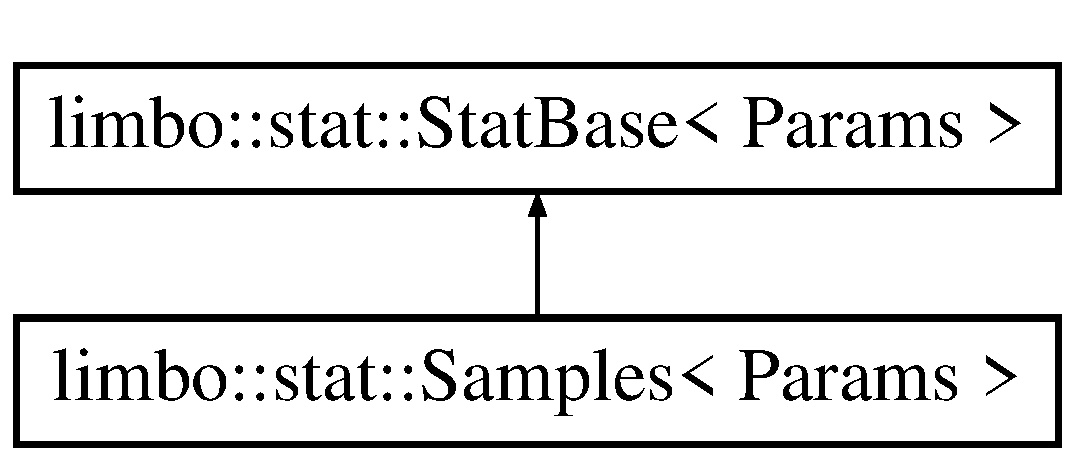
\includegraphics[height=2.000000cm]{structlimbo_1_1stat_1_1_samples}
\end{center}
\end{figure}
\subsection*{Public Member Functions}
\begin{DoxyCompactItemize}
\item 
{\footnotesize template$<$typename BO , typename Aggregator\+Function $>$ }\\void \hyperlink{structlimbo_1_1stat_1_1_samples_a456da8be91bd02cf82121d80d7531123}{operator()} (const BO \&bo, const Aggregator\+Function \&)
\end{DoxyCompactItemize}


\subsection{Detailed Description}
\subsubsection*{template$<$typename Params$>$\\*
struct limbo\+::stat\+::\+Samples$<$ Params $>$}

filename\+: {\ttfamily samples.\+dat} 

\subsection{Member Function Documentation}
\index{limbo\+::stat\+::\+Samples@{limbo\+::stat\+::\+Samples}!operator()@{operator()}}
\index{operator()@{operator()}!limbo\+::stat\+::\+Samples@{limbo\+::stat\+::\+Samples}}
\subsubsection[{\texorpdfstring{operator()(const B\+O \&bo, const Aggregator\+Function \&)}{operator()(const BO &bo, const AggregatorFunction &)}}]{\setlength{\rightskip}{0pt plus 5cm}template$<$typename Params $>$ template$<$typename BO , typename Aggregator\+Function $>$ void {\bf limbo\+::stat\+::\+Samples}$<$ Params $>$\+::operator() (
\begin{DoxyParamCaption}
\item[{const BO \&}]{bo, }
\item[{const Aggregator\+Function \&}]{}
\end{DoxyParamCaption}
)\hspace{0.3cm}{\ttfamily [inline]}}\hypertarget{structlimbo_1_1stat_1_1_samples_a456da8be91bd02cf82121d80d7531123}{}\label{structlimbo_1_1stat_1_1_samples_a456da8be91bd02cf82121d80d7531123}


The documentation for this struct was generated from the following file\+:\begin{DoxyCompactItemize}
\item 
/tmp/doc\+\_\+limbo/limbo/src/limbo/stat/\hyperlink{samples_8hpp}{samples.\+hpp}\end{DoxyCompactItemize}

\hypertarget{structrandutils_1_1seed__seq__fe}{}\section{randutils\+:\+:seed\+\_\+seq\+\_\+fe$<$ count, Int\+Rep, mix\+\_\+rounds $>$ Struct Template Reference}
\label{structrandutils_1_1seed__seq__fe}\index{randutils\+::seed\+\_\+seq\+\_\+fe$<$ count, Int\+Rep, mix\+\_\+rounds $>$@{randutils\+::seed\+\_\+seq\+\_\+fe$<$ count, Int\+Rep, mix\+\_\+rounds $>$}}


{\ttfamily \#include $<$limbo/tools/rand\+\_\+utils.\+hpp$>$}

\subsection*{Public Types}
\begin{DoxyCompactItemize}
\item 
typedef Int\+Rep \hyperlink{structrandutils_1_1seed__seq__fe_ae485fbabe93091ea392c3bf777e64279}{result\+\_\+type}
\end{DoxyCompactItemize}
\subsection*{Public Member Functions}
\begin{DoxyCompactItemize}
\item 
\hyperlink{structrandutils_1_1seed__seq__fe_adfc89fa1466e011b999baad509645b50}{seed\+\_\+seq\+\_\+fe} (const \hyperlink{structrandutils_1_1seed__seq__fe}{seed\+\_\+seq\+\_\+fe} \&)=delete
\item 
void \hyperlink{structrandutils_1_1seed__seq__fe_a117fb76a53d51b628c7ef267b47f0753}{operator=} (const \hyperlink{structrandutils_1_1seed__seq__fe}{seed\+\_\+seq\+\_\+fe} \&)=delete
\item 
{\footnotesize template$<$typename T $>$ }\\\hyperlink{structrandutils_1_1seed__seq__fe_ad716e450723c10c84a725a2e7bd0fbcd}{seed\+\_\+seq\+\_\+fe} (std\+::initializer\+\_\+list$<$ T $>$ init)
\item 
{\footnotesize template$<$typename Input\+Iter $>$ }\\\hyperlink{structrandutils_1_1seed__seq__fe_a18d0ce2ce0ac242c65e7d0aade46816e}{seed\+\_\+seq\+\_\+fe} (Input\+Iter begin, Input\+Iter end)
\item 
{\footnotesize template$<$typename Random\+Access\+Iterator $>$ }\\void \hyperlink{structrandutils_1_1seed__seq__fe_ae7622793bcbdafbeeb533413b1e3e340}{generate} (Random\+Access\+Iterator first, Random\+Access\+Iterator last) const 
\item 
{\footnotesize template$<$typename Output\+Iterator $>$ }\\void \hyperlink{structrandutils_1_1seed__seq__fe_a8b35797e2f894d92bd02cc5eb45f6915}{param} (Output\+Iterator dest) const 
\item 
{\footnotesize template$<$typename Input\+Iter $>$ }\\void \hyperlink{structrandutils_1_1seed__seq__fe_ad4b55fdb44ca51461e4e9aa9ec6aba89}{seed} (Input\+Iter begin, Input\+Iter end)
\item 
\hyperlink{structrandutils_1_1seed__seq__fe}{seed\+\_\+seq\+\_\+fe} \& \hyperlink{structrandutils_1_1seed__seq__fe_af0bd79352a6fee86f10fb4d45058ef79}{stir} ()
\end{DoxyCompactItemize}
\subsection*{Static Public Member Functions}
\begin{DoxyCompactItemize}
\item 
static constexpr size\+\_\+t \hyperlink{structrandutils_1_1seed__seq__fe_a3e9976ba5975a1ca19974cf4eaba72bc}{size} ()
\end{DoxyCompactItemize}


\subsection{Member Typedef Documentation}
\hypertarget{structrandutils_1_1seed__seq__fe_ae485fbabe93091ea392c3bf777e64279}{}\index{randutils\+::seed\+\_\+seq\+\_\+fe@{randutils\+::seed\+\_\+seq\+\_\+fe}!result\+\_\+type@{result\+\_\+type}}
\index{result\+\_\+type@{result\+\_\+type}!randutils\+::seed\+\_\+seq\+\_\+fe@{randutils\+::seed\+\_\+seq\+\_\+fe}}
\subsubsection[{result\+\_\+type}]{\setlength{\rightskip}{0pt plus 5cm}template$<$size\+\_\+t count = 4, typename Int\+Rep  = uint32\+\_\+t, size\+\_\+t mix\+\_\+rounds = 1 + (count $<$= 2)$>$ typedef Int\+Rep {\bf randutils\+::seed\+\_\+seq\+\_\+fe}$<$ count, Int\+Rep, mix\+\_\+rounds $>$\+::{\bf result\+\_\+type}}\label{structrandutils_1_1seed__seq__fe_ae485fbabe93091ea392c3bf777e64279}


\subsection{Constructor \& Destructor Documentation}
\hypertarget{structrandutils_1_1seed__seq__fe_adfc89fa1466e011b999baad509645b50}{}\index{randutils\+::seed\+\_\+seq\+\_\+fe@{randutils\+::seed\+\_\+seq\+\_\+fe}!seed\+\_\+seq\+\_\+fe@{seed\+\_\+seq\+\_\+fe}}
\index{seed\+\_\+seq\+\_\+fe@{seed\+\_\+seq\+\_\+fe}!randutils\+::seed\+\_\+seq\+\_\+fe@{randutils\+::seed\+\_\+seq\+\_\+fe}}
\subsubsection[{seed\+\_\+seq\+\_\+fe}]{\setlength{\rightskip}{0pt plus 5cm}template$<$size\+\_\+t count = 4, typename Int\+Rep  = uint32\+\_\+t, size\+\_\+t mix\+\_\+rounds = 1 + (count $<$= 2)$>$ {\bf randutils\+::seed\+\_\+seq\+\_\+fe}$<$ count, Int\+Rep, mix\+\_\+rounds $>$\+::{\bf seed\+\_\+seq\+\_\+fe} (
\begin{DoxyParamCaption}
\item[{const {\bf seed\+\_\+seq\+\_\+fe}$<$ count, Int\+Rep, mix\+\_\+rounds $>$ \&}]{}
\end{DoxyParamCaption}
)\hspace{0.3cm}{\ttfamily [delete]}}\label{structrandutils_1_1seed__seq__fe_adfc89fa1466e011b999baad509645b50}
\hypertarget{structrandutils_1_1seed__seq__fe_ad716e450723c10c84a725a2e7bd0fbcd}{}\index{randutils\+::seed\+\_\+seq\+\_\+fe@{randutils\+::seed\+\_\+seq\+\_\+fe}!seed\+\_\+seq\+\_\+fe@{seed\+\_\+seq\+\_\+fe}}
\index{seed\+\_\+seq\+\_\+fe@{seed\+\_\+seq\+\_\+fe}!randutils\+::seed\+\_\+seq\+\_\+fe@{randutils\+::seed\+\_\+seq\+\_\+fe}}
\subsubsection[{seed\+\_\+seq\+\_\+fe}]{\setlength{\rightskip}{0pt plus 5cm}template$<$size\+\_\+t count = 4, typename Int\+Rep  = uint32\+\_\+t, size\+\_\+t mix\+\_\+rounds = 1 + (count $<$= 2)$>$ template$<$typename T $>$ {\bf randutils\+::seed\+\_\+seq\+\_\+fe}$<$ count, Int\+Rep, mix\+\_\+rounds $>$\+::{\bf seed\+\_\+seq\+\_\+fe} (
\begin{DoxyParamCaption}
\item[{std\+::initializer\+\_\+list$<$ T $>$}]{init}
\end{DoxyParamCaption}
)\hspace{0.3cm}{\ttfamily [inline]}}\label{structrandutils_1_1seed__seq__fe_ad716e450723c10c84a725a2e7bd0fbcd}
\hypertarget{structrandutils_1_1seed__seq__fe_a18d0ce2ce0ac242c65e7d0aade46816e}{}\index{randutils\+::seed\+\_\+seq\+\_\+fe@{randutils\+::seed\+\_\+seq\+\_\+fe}!seed\+\_\+seq\+\_\+fe@{seed\+\_\+seq\+\_\+fe}}
\index{seed\+\_\+seq\+\_\+fe@{seed\+\_\+seq\+\_\+fe}!randutils\+::seed\+\_\+seq\+\_\+fe@{randutils\+::seed\+\_\+seq\+\_\+fe}}
\subsubsection[{seed\+\_\+seq\+\_\+fe}]{\setlength{\rightskip}{0pt plus 5cm}template$<$size\+\_\+t count = 4, typename Int\+Rep  = uint32\+\_\+t, size\+\_\+t mix\+\_\+rounds = 1 + (count $<$= 2)$>$ template$<$typename Input\+Iter $>$ {\bf randutils\+::seed\+\_\+seq\+\_\+fe}$<$ count, Int\+Rep, mix\+\_\+rounds $>$\+::{\bf seed\+\_\+seq\+\_\+fe} (
\begin{DoxyParamCaption}
\item[{Input\+Iter}]{begin, }
\item[{Input\+Iter}]{end}
\end{DoxyParamCaption}
)\hspace{0.3cm}{\ttfamily [inline]}}\label{structrandutils_1_1seed__seq__fe_a18d0ce2ce0ac242c65e7d0aade46816e}


\subsection{Member Function Documentation}
\hypertarget{structrandutils_1_1seed__seq__fe_ae7622793bcbdafbeeb533413b1e3e340}{}\index{randutils\+::seed\+\_\+seq\+\_\+fe@{randutils\+::seed\+\_\+seq\+\_\+fe}!generate@{generate}}
\index{generate@{generate}!randutils\+::seed\+\_\+seq\+\_\+fe@{randutils\+::seed\+\_\+seq\+\_\+fe}}
\subsubsection[{generate}]{\setlength{\rightskip}{0pt plus 5cm}template$<$size\+\_\+t count, typename Int\+Rep , size\+\_\+t mix\+\_\+rounds$>$ template$<$typename Random\+Access\+Iterator $>$ void {\bf randutils\+::seed\+\_\+seq\+\_\+fe}$<$ count, Int\+Rep, mix\+\_\+rounds $>$\+::generate (
\begin{DoxyParamCaption}
\item[{Random\+Access\+Iterator}]{first, }
\item[{Random\+Access\+Iterator}]{last}
\end{DoxyParamCaption}
) const}\label{structrandutils_1_1seed__seq__fe_ae7622793bcbdafbeeb533413b1e3e340}
\hypertarget{structrandutils_1_1seed__seq__fe_a117fb76a53d51b628c7ef267b47f0753}{}\index{randutils\+::seed\+\_\+seq\+\_\+fe@{randutils\+::seed\+\_\+seq\+\_\+fe}!operator=@{operator=}}
\index{operator=@{operator=}!randutils\+::seed\+\_\+seq\+\_\+fe@{randutils\+::seed\+\_\+seq\+\_\+fe}}
\subsubsection[{operator=}]{\setlength{\rightskip}{0pt plus 5cm}template$<$size\+\_\+t count = 4, typename Int\+Rep  = uint32\+\_\+t, size\+\_\+t mix\+\_\+rounds = 1 + (count $<$= 2)$>$ void {\bf randutils\+::seed\+\_\+seq\+\_\+fe}$<$ count, Int\+Rep, mix\+\_\+rounds $>$\+::operator= (
\begin{DoxyParamCaption}
\item[{const {\bf seed\+\_\+seq\+\_\+fe}$<$ count, Int\+Rep, mix\+\_\+rounds $>$ \&}]{}
\end{DoxyParamCaption}
)\hspace{0.3cm}{\ttfamily [delete]}}\label{structrandutils_1_1seed__seq__fe_a117fb76a53d51b628c7ef267b47f0753}
\hypertarget{structrandutils_1_1seed__seq__fe_a8b35797e2f894d92bd02cc5eb45f6915}{}\index{randutils\+::seed\+\_\+seq\+\_\+fe@{randutils\+::seed\+\_\+seq\+\_\+fe}!param@{param}}
\index{param@{param}!randutils\+::seed\+\_\+seq\+\_\+fe@{randutils\+::seed\+\_\+seq\+\_\+fe}}
\subsubsection[{param}]{\setlength{\rightskip}{0pt plus 5cm}template$<$size\+\_\+t count, typename Int\+Rep , size\+\_\+t mix\+\_\+rounds$>$ template$<$typename Output\+Iterator $>$ void {\bf randutils\+::seed\+\_\+seq\+\_\+fe}$<$ count, Int\+Rep, mix\+\_\+rounds $>$\+::param (
\begin{DoxyParamCaption}
\item[{Output\+Iterator}]{dest}
\end{DoxyParamCaption}
) const}\label{structrandutils_1_1seed__seq__fe_a8b35797e2f894d92bd02cc5eb45f6915}
\hypertarget{structrandutils_1_1seed__seq__fe_ad4b55fdb44ca51461e4e9aa9ec6aba89}{}\index{randutils\+::seed\+\_\+seq\+\_\+fe@{randutils\+::seed\+\_\+seq\+\_\+fe}!seed@{seed}}
\index{seed@{seed}!randutils\+::seed\+\_\+seq\+\_\+fe@{randutils\+::seed\+\_\+seq\+\_\+fe}}
\subsubsection[{seed}]{\setlength{\rightskip}{0pt plus 5cm}template$<$size\+\_\+t count = 4, typename Int\+Rep  = uint32\+\_\+t, size\+\_\+t mix\+\_\+rounds = 1 + (count $<$= 2)$>$ template$<$typename Input\+Iter $>$ void {\bf randutils\+::seed\+\_\+seq\+\_\+fe}$<$ count, Int\+Rep, mix\+\_\+rounds $>$\+::seed (
\begin{DoxyParamCaption}
\item[{Input\+Iter}]{begin, }
\item[{Input\+Iter}]{end}
\end{DoxyParamCaption}
)\hspace{0.3cm}{\ttfamily [inline]}}\label{structrandutils_1_1seed__seq__fe_ad4b55fdb44ca51461e4e9aa9ec6aba89}
\hypertarget{structrandutils_1_1seed__seq__fe_a3e9976ba5975a1ca19974cf4eaba72bc}{}\index{randutils\+::seed\+\_\+seq\+\_\+fe@{randutils\+::seed\+\_\+seq\+\_\+fe}!size@{size}}
\index{size@{size}!randutils\+::seed\+\_\+seq\+\_\+fe@{randutils\+::seed\+\_\+seq\+\_\+fe}}
\subsubsection[{size}]{\setlength{\rightskip}{0pt plus 5cm}template$<$size\+\_\+t count = 4, typename Int\+Rep  = uint32\+\_\+t, size\+\_\+t mix\+\_\+rounds = 1 + (count $<$= 2)$>$ static constexpr size\+\_\+t {\bf randutils\+::seed\+\_\+seq\+\_\+fe}$<$ count, Int\+Rep, mix\+\_\+rounds $>$\+::size (
\begin{DoxyParamCaption}
{}
\end{DoxyParamCaption}
)\hspace{0.3cm}{\ttfamily [inline]}, {\ttfamily [static]}}\label{structrandutils_1_1seed__seq__fe_a3e9976ba5975a1ca19974cf4eaba72bc}
\hypertarget{structrandutils_1_1seed__seq__fe_af0bd79352a6fee86f10fb4d45058ef79}{}\index{randutils\+::seed\+\_\+seq\+\_\+fe@{randutils\+::seed\+\_\+seq\+\_\+fe}!stir@{stir}}
\index{stir@{stir}!randutils\+::seed\+\_\+seq\+\_\+fe@{randutils\+::seed\+\_\+seq\+\_\+fe}}
\subsubsection[{stir}]{\setlength{\rightskip}{0pt plus 5cm}template$<$size\+\_\+t count = 4, typename Int\+Rep  = uint32\+\_\+t, size\+\_\+t mix\+\_\+rounds = 1 + (count $<$= 2)$>$ {\bf seed\+\_\+seq\+\_\+fe}\& {\bf randutils\+::seed\+\_\+seq\+\_\+fe}$<$ count, Int\+Rep, mix\+\_\+rounds $>$\+::stir (
\begin{DoxyParamCaption}
{}
\end{DoxyParamCaption}
)\hspace{0.3cm}{\ttfamily [inline]}}\label{structrandutils_1_1seed__seq__fe_af0bd79352a6fee86f10fb4d45058ef79}


The documentation for this struct was generated from the following file\+:\begin{DoxyCompactItemize}
\item 
/tmp/doc\+\_\+limbo/limbo/src/limbo/tools/\hyperlink{rand__utils_8hpp}{rand\+\_\+utils.\+hpp}\end{DoxyCompactItemize}

\hypertarget{structlimbo_1_1kernel_1_1_squared_exp_a_r_d}{}\section{limbo\+:\+:kernel\+:\+:Squared\+Exp\+A\+R\+D$<$ Params $>$ Struct Template Reference}
\label{structlimbo_1_1kernel_1_1_squared_exp_a_r_d}\index{limbo\+::kernel\+::\+Squared\+Exp\+A\+R\+D$<$ Params $>$@{limbo\+::kernel\+::\+Squared\+Exp\+A\+R\+D$<$ Params $>$}}


{\ttfamily \#include $<$limbo/kernel/squared\+\_\+exp\+\_\+ard.\+hpp$>$}

\subsection*{Public Member Functions}
\begin{DoxyCompactItemize}
\item 
\hyperlink{structlimbo_1_1kernel_1_1_squared_exp_a_r_d_a33d5c074a487792a305a0ae89e864f34}{Squared\+Exp\+A\+R\+D} (int dim=1)
\item 
size\+\_\+t \hyperlink{structlimbo_1_1kernel_1_1_squared_exp_a_r_d_a42d0d653ef61abce8713acdec5c876a5}{h\+\_\+params\+\_\+size} () const 
\item 
const Eigen\+::\+Vector\+Xd \& \hyperlink{structlimbo_1_1kernel_1_1_squared_exp_a_r_d_a528af96c67834d1ee6bfb8594fcc2956}{h\+\_\+params} () const 
\item 
void \hyperlink{structlimbo_1_1kernel_1_1_squared_exp_a_r_d_a0275e61c4ce395b988c903302d8e088e}{set\+\_\+h\+\_\+params} (const Eigen\+::\+Vector\+Xd \&p)
\item 
Eigen\+::\+Vector\+Xd \hyperlink{structlimbo_1_1kernel_1_1_squared_exp_a_r_d_aa7dd2fbe6e8d5e84101eb3ccce15359e}{grad} (const Eigen\+::\+Vector\+Xd \&x1, const Eigen\+::\+Vector\+Xd \&x2) const 
\item 
double \hyperlink{structlimbo_1_1kernel_1_1_squared_exp_a_r_d_ab3021822831528a6dbb4fcaf0d1c157e}{operator()} (const Eigen\+::\+Vector\+Xd \&x1, const Eigen\+::\+Vector\+Xd \&x2) const 
\item 
const Eigen\+::\+Vector\+Xd \& \hyperlink{structlimbo_1_1kernel_1_1_squared_exp_a_r_d_aad6902b522c4fdd9b5c5799a0c440c40}{ell} () const 
\end{DoxyCompactItemize}


\subsection{Detailed Description}
\subsubsection*{template$<$typename Params$>$struct limbo\+::kernel\+::\+Squared\+Exp\+A\+R\+D$<$ Params $>$}

\begin{DoxyVerb}embed:rst

Squared exponential covariance function with automatic relevance detection (to be used with a likelihood optimizer)
Computes the squared exponential covariance like this:

.. math::
    k_{SE}(x, y) = \alpha^2 \exp(-\frac{1}{2}(x-y)^T\Lambda^{-1}(x-y)),

with :math:`\Lambda = diag(l_1^2, \dots, l_n^2)` being the characteristic length scales and :math:`\alpha` describing the variability of the latent function. The parameters :math:`l_1^2, \dots, l_n^2, \alpha` are expected in this order in the parameter array.\end{DoxyVerb}
 

\subsection{Constructor \& Destructor Documentation}
\hypertarget{structlimbo_1_1kernel_1_1_squared_exp_a_r_d_a33d5c074a487792a305a0ae89e864f34}{}\index{limbo\+::kernel\+::\+Squared\+Exp\+A\+R\+D@{limbo\+::kernel\+::\+Squared\+Exp\+A\+R\+D}!Squared\+Exp\+A\+R\+D@{Squared\+Exp\+A\+R\+D}}
\index{Squared\+Exp\+A\+R\+D@{Squared\+Exp\+A\+R\+D}!limbo\+::kernel\+::\+Squared\+Exp\+A\+R\+D@{limbo\+::kernel\+::\+Squared\+Exp\+A\+R\+D}}
\subsubsection[{Squared\+Exp\+A\+R\+D}]{\setlength{\rightskip}{0pt plus 5cm}template$<$typename Params $>$ {\bf limbo\+::kernel\+::\+Squared\+Exp\+A\+R\+D}$<$ Params $>$\+::{\bf Squared\+Exp\+A\+R\+D} (
\begin{DoxyParamCaption}
\item[{int}]{dim = {\ttfamily 1}}
\end{DoxyParamCaption}
)\hspace{0.3cm}{\ttfamily [inline]}}\label{structlimbo_1_1kernel_1_1_squared_exp_a_r_d_a33d5c074a487792a305a0ae89e864f34}


\subsection{Member Function Documentation}
\hypertarget{structlimbo_1_1kernel_1_1_squared_exp_a_r_d_aad6902b522c4fdd9b5c5799a0c440c40}{}\index{limbo\+::kernel\+::\+Squared\+Exp\+A\+R\+D@{limbo\+::kernel\+::\+Squared\+Exp\+A\+R\+D}!ell@{ell}}
\index{ell@{ell}!limbo\+::kernel\+::\+Squared\+Exp\+A\+R\+D@{limbo\+::kernel\+::\+Squared\+Exp\+A\+R\+D}}
\subsubsection[{ell}]{\setlength{\rightskip}{0pt plus 5cm}template$<$typename Params $>$ const Eigen\+::\+Vector\+Xd\& {\bf limbo\+::kernel\+::\+Squared\+Exp\+A\+R\+D}$<$ Params $>$\+::ell (
\begin{DoxyParamCaption}
{}
\end{DoxyParamCaption}
) const\hspace{0.3cm}{\ttfamily [inline]}}\label{structlimbo_1_1kernel_1_1_squared_exp_a_r_d_aad6902b522c4fdd9b5c5799a0c440c40}
\hypertarget{structlimbo_1_1kernel_1_1_squared_exp_a_r_d_aa7dd2fbe6e8d5e84101eb3ccce15359e}{}\index{limbo\+::kernel\+::\+Squared\+Exp\+A\+R\+D@{limbo\+::kernel\+::\+Squared\+Exp\+A\+R\+D}!grad@{grad}}
\index{grad@{grad}!limbo\+::kernel\+::\+Squared\+Exp\+A\+R\+D@{limbo\+::kernel\+::\+Squared\+Exp\+A\+R\+D}}
\subsubsection[{grad}]{\setlength{\rightskip}{0pt plus 5cm}template$<$typename Params $>$ Eigen\+::\+Vector\+Xd {\bf limbo\+::kernel\+::\+Squared\+Exp\+A\+R\+D}$<$ Params $>$\+::grad (
\begin{DoxyParamCaption}
\item[{const Eigen\+::\+Vector\+Xd \&}]{x1, }
\item[{const Eigen\+::\+Vector\+Xd \&}]{x2}
\end{DoxyParamCaption}
) const\hspace{0.3cm}{\ttfamily [inline]}}\label{structlimbo_1_1kernel_1_1_squared_exp_a_r_d_aa7dd2fbe6e8d5e84101eb3ccce15359e}
\hypertarget{structlimbo_1_1kernel_1_1_squared_exp_a_r_d_a528af96c67834d1ee6bfb8594fcc2956}{}\index{limbo\+::kernel\+::\+Squared\+Exp\+A\+R\+D@{limbo\+::kernel\+::\+Squared\+Exp\+A\+R\+D}!h\+\_\+params@{h\+\_\+params}}
\index{h\+\_\+params@{h\+\_\+params}!limbo\+::kernel\+::\+Squared\+Exp\+A\+R\+D@{limbo\+::kernel\+::\+Squared\+Exp\+A\+R\+D}}
\subsubsection[{h\+\_\+params}]{\setlength{\rightskip}{0pt plus 5cm}template$<$typename Params $>$ const Eigen\+::\+Vector\+Xd\& {\bf limbo\+::kernel\+::\+Squared\+Exp\+A\+R\+D}$<$ Params $>$\+::h\+\_\+params (
\begin{DoxyParamCaption}
{}
\end{DoxyParamCaption}
) const\hspace{0.3cm}{\ttfamily [inline]}}\label{structlimbo_1_1kernel_1_1_squared_exp_a_r_d_a528af96c67834d1ee6bfb8594fcc2956}
\hypertarget{structlimbo_1_1kernel_1_1_squared_exp_a_r_d_a42d0d653ef61abce8713acdec5c876a5}{}\index{limbo\+::kernel\+::\+Squared\+Exp\+A\+R\+D@{limbo\+::kernel\+::\+Squared\+Exp\+A\+R\+D}!h\+\_\+params\+\_\+size@{h\+\_\+params\+\_\+size}}
\index{h\+\_\+params\+\_\+size@{h\+\_\+params\+\_\+size}!limbo\+::kernel\+::\+Squared\+Exp\+A\+R\+D@{limbo\+::kernel\+::\+Squared\+Exp\+A\+R\+D}}
\subsubsection[{h\+\_\+params\+\_\+size}]{\setlength{\rightskip}{0pt plus 5cm}template$<$typename Params $>$ size\+\_\+t {\bf limbo\+::kernel\+::\+Squared\+Exp\+A\+R\+D}$<$ Params $>$\+::h\+\_\+params\+\_\+size (
\begin{DoxyParamCaption}
{}
\end{DoxyParamCaption}
) const\hspace{0.3cm}{\ttfamily [inline]}}\label{structlimbo_1_1kernel_1_1_squared_exp_a_r_d_a42d0d653ef61abce8713acdec5c876a5}
\hypertarget{structlimbo_1_1kernel_1_1_squared_exp_a_r_d_ab3021822831528a6dbb4fcaf0d1c157e}{}\index{limbo\+::kernel\+::\+Squared\+Exp\+A\+R\+D@{limbo\+::kernel\+::\+Squared\+Exp\+A\+R\+D}!operator()@{operator()}}
\index{operator()@{operator()}!limbo\+::kernel\+::\+Squared\+Exp\+A\+R\+D@{limbo\+::kernel\+::\+Squared\+Exp\+A\+R\+D}}
\subsubsection[{operator()}]{\setlength{\rightskip}{0pt plus 5cm}template$<$typename Params $>$ double {\bf limbo\+::kernel\+::\+Squared\+Exp\+A\+R\+D}$<$ Params $>$\+::operator() (
\begin{DoxyParamCaption}
\item[{const Eigen\+::\+Vector\+Xd \&}]{x1, }
\item[{const Eigen\+::\+Vector\+Xd \&}]{x2}
\end{DoxyParamCaption}
) const\hspace{0.3cm}{\ttfamily [inline]}}\label{structlimbo_1_1kernel_1_1_squared_exp_a_r_d_ab3021822831528a6dbb4fcaf0d1c157e}
\hypertarget{structlimbo_1_1kernel_1_1_squared_exp_a_r_d_a0275e61c4ce395b988c903302d8e088e}{}\index{limbo\+::kernel\+::\+Squared\+Exp\+A\+R\+D@{limbo\+::kernel\+::\+Squared\+Exp\+A\+R\+D}!set\+\_\+h\+\_\+params@{set\+\_\+h\+\_\+params}}
\index{set\+\_\+h\+\_\+params@{set\+\_\+h\+\_\+params}!limbo\+::kernel\+::\+Squared\+Exp\+A\+R\+D@{limbo\+::kernel\+::\+Squared\+Exp\+A\+R\+D}}
\subsubsection[{set\+\_\+h\+\_\+params}]{\setlength{\rightskip}{0pt plus 5cm}template$<$typename Params $>$ void {\bf limbo\+::kernel\+::\+Squared\+Exp\+A\+R\+D}$<$ Params $>$\+::set\+\_\+h\+\_\+params (
\begin{DoxyParamCaption}
\item[{const Eigen\+::\+Vector\+Xd \&}]{p}
\end{DoxyParamCaption}
)\hspace{0.3cm}{\ttfamily [inline]}}\label{structlimbo_1_1kernel_1_1_squared_exp_a_r_d_a0275e61c4ce395b988c903302d8e088e}


The documentation for this struct was generated from the following file\+:\begin{DoxyCompactItemize}
\item 
/tmp/doc\+\_\+limbo/limbo/src/limbo/kernel/\hyperlink{squared__exp__ard_8hpp}{squared\+\_\+exp\+\_\+ard.\+hpp}\end{DoxyCompactItemize}

\hypertarget{structlimbo_1_1experimental_1_1stat_1_1defaults_1_1stat__hyper__volume}{}\section{limbo\+:\+:experimental\+:\+:stat\+:\+:defaults\+:\+:stat\+\_\+hyper\+\_\+volume Struct Reference}
\label{structlimbo_1_1experimental_1_1stat_1_1defaults_1_1stat__hyper__volume}\index{limbo\+::experimental\+::stat\+::defaults\+::stat\+\_\+hyper\+\_\+volume@{limbo\+::experimental\+::stat\+::defaults\+::stat\+\_\+hyper\+\_\+volume}}


{\ttfamily \#include $<$limbo/experimental/stat/hyper\+\_\+volume.\+hpp$>$}

\subsection*{Public Member Functions}
\begin{DoxyCompactItemize}
\item 
\hyperlink{structlimbo_1_1experimental_1_1stat_1_1defaults_1_1stat__hyper__volume_af636c73bd846f56eec5eb4d16ce27ea0}{B\+O\+\_\+\+P\+A\+R\+A\+M\+\_\+\+A\+R\+R\+AY} (double, ref, 10, 10)
\end{DoxyCompactItemize}


\subsection{Member Function Documentation}
\index{limbo\+::experimental\+::stat\+::defaults\+::stat\+\_\+hyper\+\_\+volume@{limbo\+::experimental\+::stat\+::defaults\+::stat\+\_\+hyper\+\_\+volume}!B\+O\+\_\+\+P\+A\+R\+A\+M\+\_\+\+A\+R\+R\+AY@{B\+O\+\_\+\+P\+A\+R\+A\+M\+\_\+\+A\+R\+R\+AY}}
\index{B\+O\+\_\+\+P\+A\+R\+A\+M\+\_\+\+A\+R\+R\+AY@{B\+O\+\_\+\+P\+A\+R\+A\+M\+\_\+\+A\+R\+R\+AY}!limbo\+::experimental\+::stat\+::defaults\+::stat\+\_\+hyper\+\_\+volume@{limbo\+::experimental\+::stat\+::defaults\+::stat\+\_\+hyper\+\_\+volume}}
\subsubsection[{\texorpdfstring{B\+O\+\_\+\+P\+A\+R\+A\+M\+\_\+\+A\+R\+R\+A\+Y(double, ref, 10, 10)}{BO_PARAM_ARRAY(double, ref, 10, 10)}}]{\setlength{\rightskip}{0pt plus 5cm}limbo\+::experimental\+::stat\+::defaults\+::stat\+\_\+hyper\+\_\+volume\+::\+B\+O\+\_\+\+P\+A\+R\+A\+M\+\_\+\+A\+R\+R\+AY (
\begin{DoxyParamCaption}
\item[{double}]{, }
\item[{ref}]{, }
\item[{10}]{, }
\item[{10}]{}
\end{DoxyParamCaption}
)}\hypertarget{structlimbo_1_1experimental_1_1stat_1_1defaults_1_1stat__hyper__volume_af636c73bd846f56eec5eb4d16ce27ea0}{}\label{structlimbo_1_1experimental_1_1stat_1_1defaults_1_1stat__hyper__volume_af636c73bd846f56eec5eb4d16ce27ea0}


The documentation for this struct was generated from the following file\+:\begin{DoxyCompactItemize}
\item 
/tmp/doc\+\_\+limbo/limbo/src/limbo/experimental/stat/\hyperlink{hyper__volume_8hpp}{hyper\+\_\+volume.\+hpp}\end{DoxyCompactItemize}

\hypertarget{structlimbo_1_1stat_1_1_stat_base}{}\section{limbo\+:\+:stat\+:\+:Stat\+Base$<$ Params $>$ Struct Template Reference}
\label{structlimbo_1_1stat_1_1_stat_base}\index{limbo\+::stat\+::\+Stat\+Base$<$ Params $>$@{limbo\+::stat\+::\+Stat\+Base$<$ Params $>$}}


{\ttfamily \#include $<$limbo/stat/stat\+\_\+base.\+hpp$>$}

Inheritance diagram for limbo\+:\+:stat\+:\+:Stat\+Base$<$ Params $>$\+:\begin{figure}[H]
\begin{center}
\leavevmode
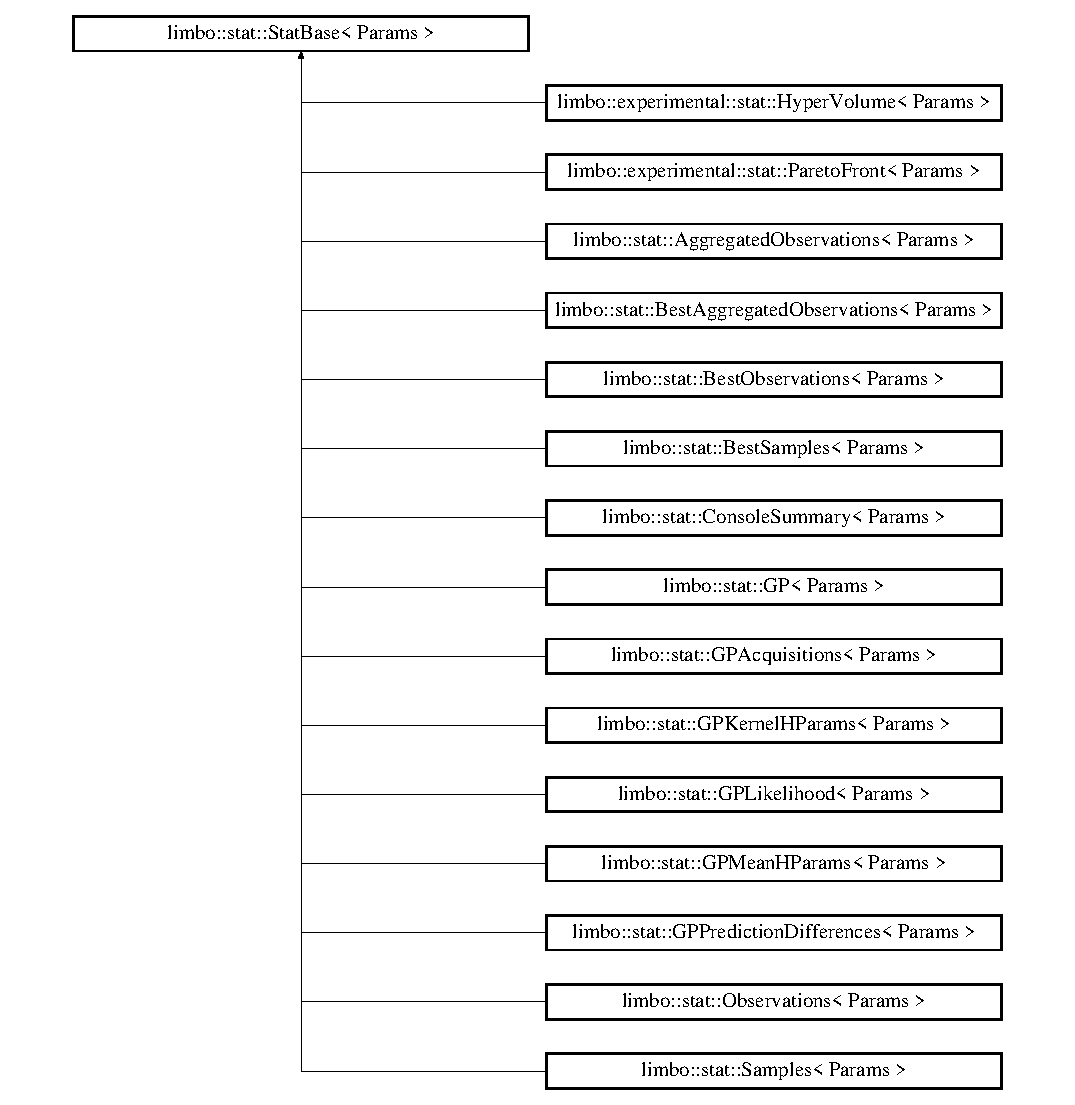
\includegraphics[height=12.000000cm]{structlimbo_1_1stat_1_1_stat_base}
\end{center}
\end{figure}
\subsection*{Public Member Functions}
\begin{DoxyCompactItemize}
\item 
\hyperlink{structlimbo_1_1stat_1_1_stat_base_aac1bea59acf624ed728660823189006f}{Stat\+Base} ()
\item 
{\footnotesize template$<$typename BO $>$ }\\void \hyperlink{structlimbo_1_1stat_1_1_stat_base_a0d2a96eb80930e66a2d374160a20b040}{operator()} (const BO \&bo)
\begin{DoxyCompactList}\small\item\em main method (to be written in derived classes) \end{DoxyCompactList}\end{DoxyCompactItemize}


\subsection{Detailed Description}
\subsubsection*{template$<$typename Params$>$\\*
struct limbo\+::stat\+::\+Stat\+Base$<$ Params $>$}

Base class for statistics

The only method provided is protected \+:

\begin{DoxyVerb}embed:rst
.. code-block:: cpp

  template <typename BO>
  void _create_log_file(const BO& bo, const std::string& name)


This method allocates an attribute `_log_file` (type: `std::shared_ptr<std::ofstream>`) if it has not been created yet, and does nothing otherwise. This method is designed so that you can safely call it in operator() while being 'guaranteed' that the file exists. Using this method is not mandatory for a statistics class.
\end{DoxyVerb}
 

\subsection{Constructor \& Destructor Documentation}
\index{limbo\+::stat\+::\+Stat\+Base@{limbo\+::stat\+::\+Stat\+Base}!Stat\+Base@{Stat\+Base}}
\index{Stat\+Base@{Stat\+Base}!limbo\+::stat\+::\+Stat\+Base@{limbo\+::stat\+::\+Stat\+Base}}
\subsubsection[{\texorpdfstring{Stat\+Base()}{StatBase()}}]{\setlength{\rightskip}{0pt plus 5cm}template$<$typename Params $>$ {\bf limbo\+::stat\+::\+Stat\+Base}$<$ Params $>$\+::{\bf Stat\+Base} (
\begin{DoxyParamCaption}
{}
\end{DoxyParamCaption}
)\hspace{0.3cm}{\ttfamily [inline]}}\hypertarget{structlimbo_1_1stat_1_1_stat_base_aac1bea59acf624ed728660823189006f}{}\label{structlimbo_1_1stat_1_1_stat_base_aac1bea59acf624ed728660823189006f}


\subsection{Member Function Documentation}
\index{limbo\+::stat\+::\+Stat\+Base@{limbo\+::stat\+::\+Stat\+Base}!operator()@{operator()}}
\index{operator()@{operator()}!limbo\+::stat\+::\+Stat\+Base@{limbo\+::stat\+::\+Stat\+Base}}
\subsubsection[{\texorpdfstring{operator()(const B\+O \&bo)}{operator()(const BO &bo)}}]{\setlength{\rightskip}{0pt plus 5cm}template$<$typename Params $>$ template$<$typename BO $>$ void {\bf limbo\+::stat\+::\+Stat\+Base}$<$ Params $>$\+::operator() (
\begin{DoxyParamCaption}
\item[{const BO \&}]{bo}
\end{DoxyParamCaption}
)\hspace{0.3cm}{\ttfamily [inline]}}\hypertarget{structlimbo_1_1stat_1_1_stat_base_a0d2a96eb80930e66a2d374160a20b040}{}\label{structlimbo_1_1stat_1_1_stat_base_a0d2a96eb80930e66a2d374160a20b040}


main method (to be written in derived classes) 



The documentation for this struct was generated from the following file\+:\begin{DoxyCompactItemize}
\item 
/tmp/doc\+\_\+limbo/limbo/src/limbo/stat/\hyperlink{stat__base_8hpp}{stat\+\_\+base.\+hpp}\end{DoxyCompactItemize}

\hypertarget{structlimbo_1_1defaults_1_1stop__maxiterations}{}\section{limbo\+:\+:defaults\+:\+:stop\+\_\+maxiterations Struct Reference}
\label{structlimbo_1_1defaults_1_1stop__maxiterations}\index{limbo\+::defaults\+::stop\+\_\+maxiterations@{limbo\+::defaults\+::stop\+\_\+maxiterations}}


{\ttfamily \#include $<$limbo/stop/max\+\_\+iterations.\+hpp$>$}

\subsection*{Public Member Functions}
\begin{DoxyCompactItemize}
\item 
\hyperlink{group__stop__defaults_ga87b011bd30622aa8b333b0d3452412ad}{B\+O\+\_\+\+P\+A\+R\+AM} (int, iterations, 190)
\end{DoxyCompactItemize}


The documentation for this struct was generated from the following file\+:\begin{DoxyCompactItemize}
\item 
/tmp/doc\+\_\+limbo/limbo/src/limbo/stop/\hyperlink{max__iterations_8hpp}{max\+\_\+iterations.\+hpp}\end{DoxyCompactItemize}

\hypertarget{structlimbo_1_1defaults_1_1stop__maxpredictedvalue}{}\section{limbo\+:\+:defaults\+:\+:stop\+\_\+maxpredictedvalue Struct Reference}
\label{structlimbo_1_1defaults_1_1stop__maxpredictedvalue}\index{limbo\+::defaults\+::stop\+\_\+maxpredictedvalue@{limbo\+::defaults\+::stop\+\_\+maxpredictedvalue}}


{\ttfamily \#include $<$limbo/stop/max\+\_\+predicted\+\_\+value.\+hpp$>$}

\subsection*{Public Member Functions}
\begin{DoxyCompactItemize}
\item 
\hyperlink{group__stop__defaults_ga65d82b10cd35e92f2df32c2dbed0f91b}{B\+O\+\_\+\+P\+A\+R\+A\+M} (double, ratio, 0.\+9)
\end{DoxyCompactItemize}


The documentation for this struct was generated from the following file\+:\begin{DoxyCompactItemize}
\item 
/tmp/doc\+\_\+limbo/limbo/src/limbo/stop/\hyperlink{max__predicted__value_8hpp}{max\+\_\+predicted\+\_\+value.\+hpp}\end{DoxyCompactItemize}

\hypertarget{structlimbo_1_1bayes__opt_1_1experimental_1_1_tree_node}{}\section{limbo\+:\+:bayes\+\_\+opt\+:\+:experimental\+:\+:Tree\+Node Struct Reference}
\label{structlimbo_1_1bayes__opt_1_1experimental_1_1_tree_node}\index{limbo\+::bayes\+\_\+opt\+::experimental\+::\+Tree\+Node@{limbo\+::bayes\+\_\+opt\+::experimental\+::\+Tree\+Node}}


{\ttfamily \#include $<$limbo/experimental/bayes\+\_\+opt/imgpo.\+hpp$>$}

\subsection*{Public Attributes}
\begin{DoxyCompactItemize}
\item 
std\+::vector$<$ Eigen\+::\+Vector\+Xd $>$ \hyperlink{structlimbo_1_1bayes__opt_1_1experimental_1_1_tree_node_a3948f2f233995ce1cd4b36d3944b27b9}{x\+\_\+max}
\item 
std\+::vector$<$ Eigen\+::\+Vector\+Xd $>$ \hyperlink{structlimbo_1_1bayes__opt_1_1experimental_1_1_tree_node_a09ee8e7b77c04a859ecdc253329303f4}{x\+\_\+min}
\item 
std\+::vector$<$ Eigen\+::\+Vector\+Xd $>$ \hyperlink{structlimbo_1_1bayes__opt_1_1experimental_1_1_tree_node_a790ebef4a33235acf40cf745599c4afe}{x}
\item 
std\+::vector$<$ Eigen\+::\+Vector\+Xd $>$ \hyperlink{structlimbo_1_1bayes__opt_1_1experimental_1_1_tree_node_a5c863b76ba45e3eefd34b8a284f7a892}{f}
\item 
std\+::vector$<$ bool $>$ \hyperlink{structlimbo_1_1bayes__opt_1_1experimental_1_1_tree_node_a69aca1e19bb631e4a5fee776f6965cd9}{leaf}
\item 
std\+::vector$<$ bool $>$ \hyperlink{structlimbo_1_1bayes__opt_1_1experimental_1_1_tree_node_a6f0c0d02a8129c2bd08ba8ecc1f9f0f1}{samp}
\end{DoxyCompactItemize}


\subsection{Member Data Documentation}
\index{limbo\+::bayes\+\_\+opt\+::experimental\+::\+Tree\+Node@{limbo\+::bayes\+\_\+opt\+::experimental\+::\+Tree\+Node}!f@{f}}
\index{f@{f}!limbo\+::bayes\+\_\+opt\+::experimental\+::\+Tree\+Node@{limbo\+::bayes\+\_\+opt\+::experimental\+::\+Tree\+Node}}
\subsubsection[{\texorpdfstring{f}{f}}]{\setlength{\rightskip}{0pt plus 5cm}std\+::vector$<$Eigen\+::\+Vector\+Xd$>$ limbo\+::bayes\+\_\+opt\+::experimental\+::\+Tree\+Node\+::f}\hypertarget{structlimbo_1_1bayes__opt_1_1experimental_1_1_tree_node_a5c863b76ba45e3eefd34b8a284f7a892}{}\label{structlimbo_1_1bayes__opt_1_1experimental_1_1_tree_node_a5c863b76ba45e3eefd34b8a284f7a892}
\index{limbo\+::bayes\+\_\+opt\+::experimental\+::\+Tree\+Node@{limbo\+::bayes\+\_\+opt\+::experimental\+::\+Tree\+Node}!leaf@{leaf}}
\index{leaf@{leaf}!limbo\+::bayes\+\_\+opt\+::experimental\+::\+Tree\+Node@{limbo\+::bayes\+\_\+opt\+::experimental\+::\+Tree\+Node}}
\subsubsection[{\texorpdfstring{leaf}{leaf}}]{\setlength{\rightskip}{0pt plus 5cm}std\+::vector$<$bool$>$ limbo\+::bayes\+\_\+opt\+::experimental\+::\+Tree\+Node\+::leaf}\hypertarget{structlimbo_1_1bayes__opt_1_1experimental_1_1_tree_node_a69aca1e19bb631e4a5fee776f6965cd9}{}\label{structlimbo_1_1bayes__opt_1_1experimental_1_1_tree_node_a69aca1e19bb631e4a5fee776f6965cd9}
\index{limbo\+::bayes\+\_\+opt\+::experimental\+::\+Tree\+Node@{limbo\+::bayes\+\_\+opt\+::experimental\+::\+Tree\+Node}!samp@{samp}}
\index{samp@{samp}!limbo\+::bayes\+\_\+opt\+::experimental\+::\+Tree\+Node@{limbo\+::bayes\+\_\+opt\+::experimental\+::\+Tree\+Node}}
\subsubsection[{\texorpdfstring{samp}{samp}}]{\setlength{\rightskip}{0pt plus 5cm}std\+::vector$<$bool$>$ limbo\+::bayes\+\_\+opt\+::experimental\+::\+Tree\+Node\+::samp}\hypertarget{structlimbo_1_1bayes__opt_1_1experimental_1_1_tree_node_a6f0c0d02a8129c2bd08ba8ecc1f9f0f1}{}\label{structlimbo_1_1bayes__opt_1_1experimental_1_1_tree_node_a6f0c0d02a8129c2bd08ba8ecc1f9f0f1}
\index{limbo\+::bayes\+\_\+opt\+::experimental\+::\+Tree\+Node@{limbo\+::bayes\+\_\+opt\+::experimental\+::\+Tree\+Node}!x@{x}}
\index{x@{x}!limbo\+::bayes\+\_\+opt\+::experimental\+::\+Tree\+Node@{limbo\+::bayes\+\_\+opt\+::experimental\+::\+Tree\+Node}}
\subsubsection[{\texorpdfstring{x}{x}}]{\setlength{\rightskip}{0pt plus 5cm}std\+::vector$<$Eigen\+::\+Vector\+Xd$>$ limbo\+::bayes\+\_\+opt\+::experimental\+::\+Tree\+Node\+::x}\hypertarget{structlimbo_1_1bayes__opt_1_1experimental_1_1_tree_node_a790ebef4a33235acf40cf745599c4afe}{}\label{structlimbo_1_1bayes__opt_1_1experimental_1_1_tree_node_a790ebef4a33235acf40cf745599c4afe}
\index{limbo\+::bayes\+\_\+opt\+::experimental\+::\+Tree\+Node@{limbo\+::bayes\+\_\+opt\+::experimental\+::\+Tree\+Node}!x\+\_\+max@{x\+\_\+max}}
\index{x\+\_\+max@{x\+\_\+max}!limbo\+::bayes\+\_\+opt\+::experimental\+::\+Tree\+Node@{limbo\+::bayes\+\_\+opt\+::experimental\+::\+Tree\+Node}}
\subsubsection[{\texorpdfstring{x\+\_\+max}{x_max}}]{\setlength{\rightskip}{0pt plus 5cm}std\+::vector$<$Eigen\+::\+Vector\+Xd$>$ limbo\+::bayes\+\_\+opt\+::experimental\+::\+Tree\+Node\+::x\+\_\+max}\hypertarget{structlimbo_1_1bayes__opt_1_1experimental_1_1_tree_node_a3948f2f233995ce1cd4b36d3944b27b9}{}\label{structlimbo_1_1bayes__opt_1_1experimental_1_1_tree_node_a3948f2f233995ce1cd4b36d3944b27b9}
\index{limbo\+::bayes\+\_\+opt\+::experimental\+::\+Tree\+Node@{limbo\+::bayes\+\_\+opt\+::experimental\+::\+Tree\+Node}!x\+\_\+min@{x\+\_\+min}}
\index{x\+\_\+min@{x\+\_\+min}!limbo\+::bayes\+\_\+opt\+::experimental\+::\+Tree\+Node@{limbo\+::bayes\+\_\+opt\+::experimental\+::\+Tree\+Node}}
\subsubsection[{\texorpdfstring{x\+\_\+min}{x_min}}]{\setlength{\rightskip}{0pt plus 5cm}std\+::vector$<$Eigen\+::\+Vector\+Xd$>$ limbo\+::bayes\+\_\+opt\+::experimental\+::\+Tree\+Node\+::x\+\_\+min}\hypertarget{structlimbo_1_1bayes__opt_1_1experimental_1_1_tree_node_a09ee8e7b77c04a859ecdc253329303f4}{}\label{structlimbo_1_1bayes__opt_1_1experimental_1_1_tree_node_a09ee8e7b77c04a859ecdc253329303f4}


The documentation for this struct was generated from the following file\+:\begin{DoxyCompactItemize}
\item 
/tmp/doc\+\_\+limbo/limbo/src/limbo/experimental/bayes\+\_\+opt/\hyperlink{imgpo_8hpp}{imgpo.\+hpp}\end{DoxyCompactItemize}

\hypertarget{classlimbo_1_1acqui_1_1_u_c_b}{}\section{limbo\+:\+:acqui\+:\+:U\+C\+B$<$ Params, Model $>$ Class Template Reference}
\label{classlimbo_1_1acqui_1_1_u_c_b}\index{limbo\+::acqui\+::\+U\+C\+B$<$ Params, Model $>$@{limbo\+::acqui\+::\+U\+C\+B$<$ Params, Model $>$}}


{\ttfamily \#include $<$limbo/acqui/ucb.\+hpp$>$}

\subsection*{Public Member Functions}
\begin{DoxyCompactItemize}
\item 
\hyperlink{classlimbo_1_1acqui_1_1_u_c_b_ae4410ba09273ea88b36130ea916fcc60}{U\+C\+B} (const Model \&model, int iteration=0)
\item 
size\+\_\+t \hyperlink{classlimbo_1_1acqui_1_1_u_c_b_ab922a11b709216f35db6ee83fcb86ed5}{dim\+\_\+in} () const 
\item 
size\+\_\+t \hyperlink{classlimbo_1_1acqui_1_1_u_c_b_aa6870bb7764a6f729db39f86eb005d54}{dim\+\_\+out} () const 
\item 
{\footnotesize template$<$typename Aggregator\+Function $>$ }\\\hyperlink{group__opt__tools_ga362b55973a38ac71f27a06f9d9c14f24}{opt\+::eval\+\_\+t} \hyperlink{classlimbo_1_1acqui_1_1_u_c_b_a029c5489c29e294e50e0d83a203c9572}{operator()} (const Eigen\+::\+Vector\+Xd \&v, const Aggregator\+Function \&afun, bool gradient) const 
\end{DoxyCompactItemize}


\subsection{Detailed Description}
\subsubsection*{template$<$typename Params, typename Model$>$class limbo\+::acqui\+::\+U\+C\+B$<$ Params, Model $>$}

\begin{DoxyVerb}embed:rst
Classic UCB (Upper Confidence Bound). See :cite:`brochu2010tutorial`, p. 14

  .. math::
    UCB(x) = \mu(x) + \alpha \sigma(x).

Parameters:
  - ``double alpha``
\end{DoxyVerb}
 

\subsection{Constructor \& Destructor Documentation}
\hypertarget{classlimbo_1_1acqui_1_1_u_c_b_ae4410ba09273ea88b36130ea916fcc60}{}\index{limbo\+::acqui\+::\+U\+C\+B@{limbo\+::acqui\+::\+U\+C\+B}!U\+C\+B@{U\+C\+B}}
\index{U\+C\+B@{U\+C\+B}!limbo\+::acqui\+::\+U\+C\+B@{limbo\+::acqui\+::\+U\+C\+B}}
\subsubsection[{U\+C\+B}]{\setlength{\rightskip}{0pt plus 5cm}template$<$typename Params , typename Model $>$ {\bf limbo\+::acqui\+::\+U\+C\+B}$<$ Params, Model $>$\+::{\bf U\+C\+B} (
\begin{DoxyParamCaption}
\item[{const Model \&}]{model, }
\item[{int}]{iteration = {\ttfamily 0}}
\end{DoxyParamCaption}
)\hspace{0.3cm}{\ttfamily [inline]}}\label{classlimbo_1_1acqui_1_1_u_c_b_ae4410ba09273ea88b36130ea916fcc60}


\subsection{Member Function Documentation}
\hypertarget{classlimbo_1_1acqui_1_1_u_c_b_ab922a11b709216f35db6ee83fcb86ed5}{}\index{limbo\+::acqui\+::\+U\+C\+B@{limbo\+::acqui\+::\+U\+C\+B}!dim\+\_\+in@{dim\+\_\+in}}
\index{dim\+\_\+in@{dim\+\_\+in}!limbo\+::acqui\+::\+U\+C\+B@{limbo\+::acqui\+::\+U\+C\+B}}
\subsubsection[{dim\+\_\+in}]{\setlength{\rightskip}{0pt plus 5cm}template$<$typename Params , typename Model $>$ size\+\_\+t {\bf limbo\+::acqui\+::\+U\+C\+B}$<$ Params, Model $>$\+::dim\+\_\+in (
\begin{DoxyParamCaption}
{}
\end{DoxyParamCaption}
) const\hspace{0.3cm}{\ttfamily [inline]}}\label{classlimbo_1_1acqui_1_1_u_c_b_ab922a11b709216f35db6ee83fcb86ed5}
\hypertarget{classlimbo_1_1acqui_1_1_u_c_b_aa6870bb7764a6f729db39f86eb005d54}{}\index{limbo\+::acqui\+::\+U\+C\+B@{limbo\+::acqui\+::\+U\+C\+B}!dim\+\_\+out@{dim\+\_\+out}}
\index{dim\+\_\+out@{dim\+\_\+out}!limbo\+::acqui\+::\+U\+C\+B@{limbo\+::acqui\+::\+U\+C\+B}}
\subsubsection[{dim\+\_\+out}]{\setlength{\rightskip}{0pt plus 5cm}template$<$typename Params , typename Model $>$ size\+\_\+t {\bf limbo\+::acqui\+::\+U\+C\+B}$<$ Params, Model $>$\+::dim\+\_\+out (
\begin{DoxyParamCaption}
{}
\end{DoxyParamCaption}
) const\hspace{0.3cm}{\ttfamily [inline]}}\label{classlimbo_1_1acqui_1_1_u_c_b_aa6870bb7764a6f729db39f86eb005d54}
\hypertarget{classlimbo_1_1acqui_1_1_u_c_b_a029c5489c29e294e50e0d83a203c9572}{}\index{limbo\+::acqui\+::\+U\+C\+B@{limbo\+::acqui\+::\+U\+C\+B}!operator()@{operator()}}
\index{operator()@{operator()}!limbo\+::acqui\+::\+U\+C\+B@{limbo\+::acqui\+::\+U\+C\+B}}
\subsubsection[{operator()}]{\setlength{\rightskip}{0pt plus 5cm}template$<$typename Params , typename Model $>$ template$<$typename Aggregator\+Function $>$ {\bf opt\+::eval\+\_\+t} {\bf limbo\+::acqui\+::\+U\+C\+B}$<$ Params, Model $>$\+::operator() (
\begin{DoxyParamCaption}
\item[{const Eigen\+::\+Vector\+Xd \&}]{v, }
\item[{const Aggregator\+Function \&}]{afun, }
\item[{bool}]{gradient}
\end{DoxyParamCaption}
) const\hspace{0.3cm}{\ttfamily [inline]}}\label{classlimbo_1_1acqui_1_1_u_c_b_a029c5489c29e294e50e0d83a203c9572}


The documentation for this class was generated from the following file\+:\begin{DoxyCompactItemize}
\item 
/tmp/doc\+\_\+limbo/limbo/src/limbo/acqui/\hyperlink{ucb_8hpp}{ucb.\+hpp}\end{DoxyCompactItemize}

\hypertarget{classlimbo_1_1acqui_1_1experimental_1_1_u_c_b___i_m_g_p_o}{}\section{limbo\+:\+:acqui\+:\+:experimental\+:\+:U\+C\+B\+\_\+\+I\+M\+G\+PO$<$ Params, Model $>$ Class Template Reference}
\label{classlimbo_1_1acqui_1_1experimental_1_1_u_c_b___i_m_g_p_o}\index{limbo\+::acqui\+::experimental\+::\+U\+C\+B\+\_\+\+I\+M\+G\+P\+O$<$ Params, Model $>$@{limbo\+::acqui\+::experimental\+::\+U\+C\+B\+\_\+\+I\+M\+G\+P\+O$<$ Params, Model $>$}}


{\ttfamily \#include $<$limbo/experimental/acqui/ucb\+\_\+imgpo.\+hpp$>$}

\subsection*{Public Member Functions}
\begin{DoxyCompactItemize}
\item 
\hyperlink{classlimbo_1_1acqui_1_1experimental_1_1_u_c_b___i_m_g_p_o_a13c9d89758fe241c051fafe06337fd1e}{U\+C\+B\+\_\+\+I\+M\+G\+PO} (const Model \&model, size\+\_\+t M=1)
\item 
size\+\_\+t \hyperlink{classlimbo_1_1acqui_1_1experimental_1_1_u_c_b___i_m_g_p_o_ac773917d0802053632cd37e7885fe282}{dim\+\_\+in} () const 
\item 
size\+\_\+t \hyperlink{classlimbo_1_1acqui_1_1experimental_1_1_u_c_b___i_m_g_p_o_ad6b61ac04acf5a268eb7fef4a879bc31}{dim\+\_\+out} () const 
\item 
{\footnotesize template$<$typename Aggregator\+Function $>$ }\\double \hyperlink{classlimbo_1_1acqui_1_1experimental_1_1_u_c_b___i_m_g_p_o_a4f0d0671883e2d3a9a501e95c091098f}{operator()} (const Eigen\+::\+Vector\+Xd \&v, const Aggregator\+Function \&afun) const 
\end{DoxyCompactItemize}


\subsection{Constructor \& Destructor Documentation}
\index{limbo\+::acqui\+::experimental\+::\+U\+C\+B\+\_\+\+I\+M\+G\+PO@{limbo\+::acqui\+::experimental\+::\+U\+C\+B\+\_\+\+I\+M\+G\+PO}!U\+C\+B\+\_\+\+I\+M\+G\+PO@{U\+C\+B\+\_\+\+I\+M\+G\+PO}}
\index{U\+C\+B\+\_\+\+I\+M\+G\+PO@{U\+C\+B\+\_\+\+I\+M\+G\+PO}!limbo\+::acqui\+::experimental\+::\+U\+C\+B\+\_\+\+I\+M\+G\+PO@{limbo\+::acqui\+::experimental\+::\+U\+C\+B\+\_\+\+I\+M\+G\+PO}}
\subsubsection[{\texorpdfstring{U\+C\+B\+\_\+\+I\+M\+G\+P\+O(const Model \&model, size\+\_\+t M=1)}{UCB_IMGPO(const Model &model, size_t M=1)}}]{\setlength{\rightskip}{0pt plus 5cm}template$<$typename Params , typename Model $>$ {\bf limbo\+::acqui\+::experimental\+::\+U\+C\+B\+\_\+\+I\+M\+G\+PO}$<$ Params, Model $>$\+::{\bf U\+C\+B\+\_\+\+I\+M\+G\+PO} (
\begin{DoxyParamCaption}
\item[{const Model \&}]{model, }
\item[{size\+\_\+t}]{M = {\ttfamily 1}}
\end{DoxyParamCaption}
)\hspace{0.3cm}{\ttfamily [inline]}}\hypertarget{classlimbo_1_1acqui_1_1experimental_1_1_u_c_b___i_m_g_p_o_a13c9d89758fe241c051fafe06337fd1e}{}\label{classlimbo_1_1acqui_1_1experimental_1_1_u_c_b___i_m_g_p_o_a13c9d89758fe241c051fafe06337fd1e}


\subsection{Member Function Documentation}
\index{limbo\+::acqui\+::experimental\+::\+U\+C\+B\+\_\+\+I\+M\+G\+PO@{limbo\+::acqui\+::experimental\+::\+U\+C\+B\+\_\+\+I\+M\+G\+PO}!dim\+\_\+in@{dim\+\_\+in}}
\index{dim\+\_\+in@{dim\+\_\+in}!limbo\+::acqui\+::experimental\+::\+U\+C\+B\+\_\+\+I\+M\+G\+PO@{limbo\+::acqui\+::experimental\+::\+U\+C\+B\+\_\+\+I\+M\+G\+PO}}
\subsubsection[{\texorpdfstring{dim\+\_\+in() const }{dim_in() const }}]{\setlength{\rightskip}{0pt plus 5cm}template$<$typename Params , typename Model $>$ size\+\_\+t {\bf limbo\+::acqui\+::experimental\+::\+U\+C\+B\+\_\+\+I\+M\+G\+PO}$<$ Params, Model $>$\+::dim\+\_\+in (
\begin{DoxyParamCaption}
{}
\end{DoxyParamCaption}
) const\hspace{0.3cm}{\ttfamily [inline]}}\hypertarget{classlimbo_1_1acqui_1_1experimental_1_1_u_c_b___i_m_g_p_o_ac773917d0802053632cd37e7885fe282}{}\label{classlimbo_1_1acqui_1_1experimental_1_1_u_c_b___i_m_g_p_o_ac773917d0802053632cd37e7885fe282}
\index{limbo\+::acqui\+::experimental\+::\+U\+C\+B\+\_\+\+I\+M\+G\+PO@{limbo\+::acqui\+::experimental\+::\+U\+C\+B\+\_\+\+I\+M\+G\+PO}!dim\+\_\+out@{dim\+\_\+out}}
\index{dim\+\_\+out@{dim\+\_\+out}!limbo\+::acqui\+::experimental\+::\+U\+C\+B\+\_\+\+I\+M\+G\+PO@{limbo\+::acqui\+::experimental\+::\+U\+C\+B\+\_\+\+I\+M\+G\+PO}}
\subsubsection[{\texorpdfstring{dim\+\_\+out() const }{dim_out() const }}]{\setlength{\rightskip}{0pt plus 5cm}template$<$typename Params , typename Model $>$ size\+\_\+t {\bf limbo\+::acqui\+::experimental\+::\+U\+C\+B\+\_\+\+I\+M\+G\+PO}$<$ Params, Model $>$\+::dim\+\_\+out (
\begin{DoxyParamCaption}
{}
\end{DoxyParamCaption}
) const\hspace{0.3cm}{\ttfamily [inline]}}\hypertarget{classlimbo_1_1acqui_1_1experimental_1_1_u_c_b___i_m_g_p_o_ad6b61ac04acf5a268eb7fef4a879bc31}{}\label{classlimbo_1_1acqui_1_1experimental_1_1_u_c_b___i_m_g_p_o_ad6b61ac04acf5a268eb7fef4a879bc31}
\index{limbo\+::acqui\+::experimental\+::\+U\+C\+B\+\_\+\+I\+M\+G\+PO@{limbo\+::acqui\+::experimental\+::\+U\+C\+B\+\_\+\+I\+M\+G\+PO}!operator()@{operator()}}
\index{operator()@{operator()}!limbo\+::acqui\+::experimental\+::\+U\+C\+B\+\_\+\+I\+M\+G\+PO@{limbo\+::acqui\+::experimental\+::\+U\+C\+B\+\_\+\+I\+M\+G\+PO}}
\subsubsection[{\texorpdfstring{operator()(const Eigen\+::\+Vector\+Xd \&v, const Aggregator\+Function \&afun) const }{operator()(const Eigen::VectorXd &v, const AggregatorFunction &afun) const }}]{\setlength{\rightskip}{0pt plus 5cm}template$<$typename Params , typename Model $>$ template$<$typename Aggregator\+Function $>$ double {\bf limbo\+::acqui\+::experimental\+::\+U\+C\+B\+\_\+\+I\+M\+G\+PO}$<$ Params, Model $>$\+::operator() (
\begin{DoxyParamCaption}
\item[{const Eigen\+::\+Vector\+Xd \&}]{v, }
\item[{const Aggregator\+Function \&}]{afun}
\end{DoxyParamCaption}
) const\hspace{0.3cm}{\ttfamily [inline]}}\hypertarget{classlimbo_1_1acqui_1_1experimental_1_1_u_c_b___i_m_g_p_o_a4f0d0671883e2d3a9a501e95c091098f}{}\label{classlimbo_1_1acqui_1_1experimental_1_1_u_c_b___i_m_g_p_o_a4f0d0671883e2d3a9a501e95c091098f}


The documentation for this class was generated from the following file\+:\begin{DoxyCompactItemize}
\item 
/tmp/doc\+\_\+limbo/limbo/src/limbo/experimental/acqui/\hyperlink{ucb__imgpo_8hpp}{ucb\+\_\+imgpo.\+hpp}\end{DoxyCompactItemize}

\chapter{File Documentation}
\hypertarget{acqui_8hpp}{}\section{/tmp/doc\+\_\+limbo/limbo/src/limbo/acqui.hpp File Reference}
\label{acqui_8hpp}\index{/tmp/doc\+\_\+limbo/limbo/src/limbo/acqui.\+hpp@{/tmp/doc\+\_\+limbo/limbo/src/limbo/acqui.\+hpp}}
{\ttfamily \#include $<$limbo/acqui/ucb.\+hpp$>$}\\*
{\ttfamily \#include $<$limbo/acqui/gp\+\_\+ucb.\+hpp$>$}\\*

\hypertarget{gp__ucb_8hpp}{}\section{/tmp/doc\+\_\+limbo/limbo/src/limbo/acqui/gp\+\_\+ucb.hpp File Reference}
\label{gp__ucb_8hpp}\index{/tmp/doc\+\_\+limbo/limbo/src/limbo/acqui/gp\+\_\+ucb.\+hpp@{/tmp/doc\+\_\+limbo/limbo/src/limbo/acqui/gp\+\_\+ucb.\+hpp}}
{\ttfamily \#include $<$Eigen/\+Core$>$}\\*
{\ttfamily \#include $<$limbo/tools/macros.\+hpp$>$}\\*
\subsection*{Classes}
\begin{DoxyCompactItemize}
\item 
struct \hyperlink{structlimbo_1_1defaults_1_1acqui__gpucb}{limbo\+::defaults\+::acqui\+\_\+gpucb}
\item 
class \hyperlink{classlimbo_1_1acqui_1_1_g_p___u_c_b}{limbo\+::acqui\+::\+G\+P\+\_\+\+U\+C\+B$<$ Params, Model $>$}
\end{DoxyCompactItemize}
\subsection*{Namespaces}
\begin{DoxyCompactItemize}
\item 
 \hyperlink{namespacelimbo}{limbo}
\item 
 \hyperlink{namespacelimbo_1_1defaults}{limbo\+::defaults}
\item 
 \hyperlink{namespacelimbo_1_1acqui}{limbo\+::acqui}
\end{DoxyCompactItemize}

\hypertarget{ucb_8hpp}{}\section{/tmp/doc\+\_\+limbo/limbo/src/limbo/acqui/ucb.hpp File Reference}
\label{ucb_8hpp}\index{/tmp/doc\+\_\+limbo/limbo/src/limbo/acqui/ucb.\+hpp@{/tmp/doc\+\_\+limbo/limbo/src/limbo/acqui/ucb.\+hpp}}
{\ttfamily \#include $<$Eigen/\+Core$>$}\\*
{\ttfamily \#include $<$limbo/tools/macros.\+hpp$>$}\\*
\subsection*{Classes}
\begin{DoxyCompactItemize}
\item 
struct \hyperlink{structlimbo_1_1defaults_1_1acqui__ucb}{limbo\+::defaults\+::acqui\+\_\+ucb}
\item 
class \hyperlink{classlimbo_1_1acqui_1_1_u_c_b}{limbo\+::acqui\+::\+U\+C\+B$<$ Params, Model $>$}
\end{DoxyCompactItemize}
\subsection*{Namespaces}
\begin{DoxyCompactItemize}
\item 
 \hyperlink{namespacelimbo}{limbo}
\item 
 \hyperlink{namespacelimbo_1_1defaults}{limbo\+::defaults}
\item 
 \hyperlink{namespacelimbo_1_1acqui}{limbo\+::acqui}
\end{DoxyCompactItemize}

\hypertarget{bayes__opt_8hpp}{}\section{/tmp/doc\+\_\+limbo/limbo/src/limbo/bayes\+\_\+opt.hpp File Reference}
\label{bayes__opt_8hpp}\index{/tmp/doc\+\_\+limbo/limbo/src/limbo/bayes\+\_\+opt.\+hpp@{/tmp/doc\+\_\+limbo/limbo/src/limbo/bayes\+\_\+opt.\+hpp}}
{\ttfamily \#include $<$limbo/bayes\+\_\+opt/boptimizer.\+hpp$>$}\\*

\hypertarget{bo__base_8hpp}{}\section{/tmp/doc\+\_\+limbo/limbo/src/limbo/bayes\+\_\+opt/bo\+\_\+base.hpp File Reference}
\label{bo__base_8hpp}\index{/tmp/doc\+\_\+limbo/limbo/src/limbo/bayes\+\_\+opt/bo\+\_\+base.\+hpp@{/tmp/doc\+\_\+limbo/limbo/src/limbo/bayes\+\_\+opt/bo\+\_\+base.\+hpp}}
{\ttfamily \#include $<$vector$>$}\\*
{\ttfamily \#include $<$iostream$>$}\\*
{\ttfamily \#include $<$limits$>$}\\*
{\ttfamily \#include $<$exception$>$}\\*
{\ttfamily \#include $<$boost/parameter.\+hpp$>$}\\*
{\ttfamily \#include $<$boost/fusion/include/vector.\+hpp$>$}\\*
{\ttfamily \#include $<$boost/fusion/include/accumulate.\+hpp$>$}\\*
{\ttfamily \#include $<$boost/fusion/include/for\+\_\+each.\+hpp$>$}\\*
{\ttfamily \#include $<$boost/filesystem.\+hpp$>$}\\*
{\ttfamily \#include $<$Eigen/\+Core$>$}\\*
{\ttfamily \#include $<$limbo/tools/macros.\+hpp$>$}\\*
{\ttfamily \#include $<$limbo/stop/chain\+\_\+criteria.\+hpp$>$}\\*
{\ttfamily \#include $<$limbo/stop/max\+\_\+iterations.\+hpp$>$}\\*
{\ttfamily \#include $<$limbo/stat/samples.\+hpp$>$}\\*
{\ttfamily \#include $<$limbo/stat/aggregated\+\_\+observations.\+hpp$>$}\\*
{\ttfamily \#include $<$limbo/stat/console\+\_\+summary.\+hpp$>$}\\*
{\ttfamily \#include $<$limbo/tools/sys.\+hpp$>$}\\*
{\ttfamily \#include $<$limbo/kernel/exp.\+hpp$>$}\\*
{\ttfamily \#include $<$limbo/acqui/ucb.\+hpp$>$}\\*
{\ttfamily \#include $<$limbo/mean/data.\+hpp$>$}\\*
{\ttfamily \#include $<$limbo/model/gp.\+hpp$>$}\\*
{\ttfamily \#include $<$limbo/init/random\+\_\+sampling.\+hpp$>$}\\*
{\ttfamily \#include $<$limbo/tools/math.\+hpp$>$}\\*
\subsection*{Classes}
\begin{DoxyCompactItemize}
\item 
struct \hyperlink{structlimbo_1_1defaults_1_1bayes__opt__bobase}{limbo\+::defaults\+::bayes\+\_\+opt\+\_\+bobase}
\item 
struct \hyperlink{structlimbo_1_1_refresh_stat__f}{limbo\+::\+Refresh\+Stat\+\_\+f$<$ B\+O, Aggregator\+Function $>$}
\item 
struct \hyperlink{structlimbo_1_1_first_elem}{limbo\+::\+First\+Elem}
\item 
class \hyperlink{classlimbo_1_1_evaluation_error}{limbo\+::\+Evaluation\+Error}
\item 
class \hyperlink{classlimbo_1_1bayes__opt_1_1_bo_base}{limbo\+::bayes\+\_\+opt\+::\+Bo\+Base$<$ Params, A1, A2, A3, A4, A5, A6 $>$}
\item 
struct \hyperlink{structlimbo_1_1bayes__opt_1_1_bo_base_1_1defaults}{limbo\+::bayes\+\_\+opt\+::\+Bo\+Base$<$ Params, A1, A2, A3, A4, A5, A6 $>$\+::defaults}
\end{DoxyCompactItemize}
\subsection*{Namespaces}
\begin{DoxyCompactItemize}
\item 
 \hyperlink{namespacelimbo}{limbo}
\item 
 \hyperlink{namespacelimbo_1_1defaults}{limbo\+::defaults}
\item 
 \hyperlink{namespacelimbo_1_1bayes__opt}{limbo\+::bayes\+\_\+opt}
\end{DoxyCompactItemize}
\subsection*{Macros}
\begin{DoxyCompactItemize}
\item 
\#define \hyperlink{bo__base_8hpp_a673f164000ed2c207f200528add4f736}{B\+O\+O\+S\+T\+\_\+\+N\+O\+\_\+\+S\+C\+O\+P\+E\+D\+\_\+\+E\+N\+U\+M\+S}
\end{DoxyCompactItemize}
\subsection*{Typedefs}
\begin{DoxyCompactItemize}
\item 
using \hyperlink{namespacelimbo_1_1bayes__opt_a824303857a6912240f23e422927773f7}{limbo\+::bayes\+\_\+opt\+::bobase\+\_\+signature} = boost\+::parameter\+::parameters$<$ boost\+::parameter\+::optional$<$ tag\+::statsfun $>$, boost\+::parameter\+::optional$<$ tag\+::initfun $>$, boost\+::parameter\+::optional$<$ tag\+::acquifun $>$, boost\+::parameter\+::optional$<$ tag\+::stopcrit $>$, boost\+::parameter\+::optional$<$ tag\+::modelfun $>$$>$
\end{DoxyCompactItemize}


\subsection{Macro Definition Documentation}
\hypertarget{bo__base_8hpp_a673f164000ed2c207f200528add4f736}{}\index{bo\+\_\+base.\+hpp@{bo\+\_\+base.\+hpp}!B\+O\+O\+S\+T\+\_\+\+N\+O\+\_\+\+S\+C\+O\+P\+E\+D\+\_\+\+E\+N\+U\+M\+S@{B\+O\+O\+S\+T\+\_\+\+N\+O\+\_\+\+S\+C\+O\+P\+E\+D\+\_\+\+E\+N\+U\+M\+S}}
\index{B\+O\+O\+S\+T\+\_\+\+N\+O\+\_\+\+S\+C\+O\+P\+E\+D\+\_\+\+E\+N\+U\+M\+S@{B\+O\+O\+S\+T\+\_\+\+N\+O\+\_\+\+S\+C\+O\+P\+E\+D\+\_\+\+E\+N\+U\+M\+S}!bo\+\_\+base.\+hpp@{bo\+\_\+base.\+hpp}}
\subsubsection[{B\+O\+O\+S\+T\+\_\+\+N\+O\+\_\+\+S\+C\+O\+P\+E\+D\+\_\+\+E\+N\+U\+M\+S}]{\setlength{\rightskip}{0pt plus 5cm}\#define B\+O\+O\+S\+T\+\_\+\+N\+O\+\_\+\+S\+C\+O\+P\+E\+D\+\_\+\+E\+N\+U\+M\+S}\label{bo__base_8hpp_a673f164000ed2c207f200528add4f736}

\hypertarget{boptimizer_8hpp}{}\section{/tmp/doc\+\_\+limbo/limbo/src/limbo/bayes\+\_\+opt/boptimizer.hpp File Reference}
\label{boptimizer_8hpp}\index{/tmp/doc\+\_\+limbo/limbo/src/limbo/bayes\+\_\+opt/boptimizer.\+hpp@{/tmp/doc\+\_\+limbo/limbo/src/limbo/bayes\+\_\+opt/boptimizer.\+hpp}}
{\ttfamily \#include $<$iostream$>$}\\*
{\ttfamily \#include $<$algorithm$>$}\\*
{\ttfamily \#include $<$iterator$>$}\\*
{\ttfamily \#include $<$boost/parameter/aux\+\_\+/void.\+hpp$>$}\\*
{\ttfamily \#include $<$Eigen/\+Core$>$}\\*
{\ttfamily \#include $<$limbo/tools/macros.\+hpp$>$}\\*
{\ttfamily \#include $<$limbo/tools/random\+\_\+generator.\+hpp$>$}\\*
{\ttfamily \#include $<$limbo/bayes\+\_\+opt/bo\+\_\+base.\+hpp$>$}\\*
{\ttfamily \#include $<$limbo/opt/nlopt\+\_\+no\+\_\+grad.\+hpp$>$}\\*
\subsection*{Classes}
\begin{DoxyCompactItemize}
\item 
struct \hyperlink{structlimbo_1_1defaults_1_1bayes__opt__boptimizer}{limbo\+::defaults\+::bayes\+\_\+opt\+\_\+boptimizer}
\item 
class \hyperlink{classlimbo_1_1bayes__opt_1_1_b_optimizer}{limbo\+::bayes\+\_\+opt\+::\+B\+Optimizer$<$ Params, A1, A2, A3, A4, A5, A6 $>$}
\item 
struct \hyperlink{structlimbo_1_1bayes__opt_1_1_b_optimizer_1_1defaults}{limbo\+::bayes\+\_\+opt\+::\+B\+Optimizer$<$ Params, A1, A2, A3, A4, A5, A6 $>$\+::defaults}
\end{DoxyCompactItemize}
\subsection*{Namespaces}
\begin{DoxyCompactItemize}
\item 
 \hyperlink{namespacelimbo}{limbo}
\item 
 \hyperlink{namespacelimbo_1_1defaults}{limbo\+::defaults}
\item 
 \hyperlink{namespacelimbo_1_1bayes__opt}{limbo\+::bayes\+\_\+opt}
\end{DoxyCompactItemize}
\subsection*{Typedefs}
\begin{DoxyCompactItemize}
\item 
using \hyperlink{namespacelimbo_1_1bayes__opt_a6f7eddef5a0de80d03fe4df398480997}{limbo\+::bayes\+\_\+opt\+::boptimizer\+\_\+signature} = boost\+::parameter\+::parameters$<$ boost\+::parameter\+::optional$<$ tag\+::acquiopt $>$, boost\+::parameter\+::optional$<$ tag\+::statsfun $>$, boost\+::parameter\+::optional$<$ tag\+::initfun $>$, boost\+::parameter\+::optional$<$ tag\+::acquifun $>$, boost\+::parameter\+::optional$<$ tag\+::stopcrit $>$, boost\+::parameter\+::optional$<$ tag\+::modelfun $>$$>$
\end{DoxyCompactItemize}

\hypertarget{acqui_2ehvi_8hpp}{}\section{/tmp/doc\+\_\+limbo/limbo/src/limbo/experimental/acqui/ehvi.hpp File Reference}
\label{acqui_2ehvi_8hpp}\index{/tmp/doc\+\_\+limbo/limbo/src/limbo/experimental/acqui/ehvi.\+hpp@{/tmp/doc\+\_\+limbo/limbo/src/limbo/experimental/acqui/ehvi.\+hpp}}
{\ttfamily \#include $<$vector$>$}\\*
{\ttfamily \#include $<$Eigen/\+Core$>$}\\*
{\ttfamily \#include $<$ehvi/ehvi\+\_\+calculations.\+h$>$}\\*
\subsection*{Classes}
\begin{DoxyCompactItemize}
\item 
class \hyperlink{classlimbo_1_1acqui_1_1_ehvi}{limbo\+::acqui\+::\+Ehvi$<$ Params, Model $>$}
\end{DoxyCompactItemize}
\subsection*{Namespaces}
\begin{DoxyCompactItemize}
\item 
 \hyperlink{namespacelimbo}{limbo}
\item 
 \hyperlink{namespacelimbo_1_1acqui}{limbo\+::acqui}
\end{DoxyCompactItemize}

\hypertarget{bayes__opt_2ehvi_8hpp}{}\section{/tmp/doc\+\_\+limbo/limbo/src/limbo/experimental/bayes\+\_\+opt/ehvi.hpp File Reference}
\label{bayes__opt_2ehvi_8hpp}\index{/tmp/doc\+\_\+limbo/limbo/src/limbo/experimental/bayes\+\_\+opt/ehvi.\+hpp@{/tmp/doc\+\_\+limbo/limbo/src/limbo/experimental/bayes\+\_\+opt/ehvi.\+hpp}}
{\ttfamily \#include $<$algorithm$>$}\\*
{\ttfamily \#include $<$ehvi/ehvi\+\_\+calculations.\+h$>$}\\*
{\ttfamily \#include $<$ehvi/ehvi\+\_\+sliceupdate.\+h$>$}\\*
{\ttfamily \#include $<$limbo/tools/macros.\+hpp$>$}\\*
{\ttfamily \#include $<$limbo/experimental/bayes\+\_\+opt/bo\+\_\+multi.\+hpp$>$}\\*
{\ttfamily \#include $<$limbo/experimental/acqui/ehvi.\+hpp$>$}\\*
\subsection*{Classes}
\begin{DoxyCompactItemize}
\item 
struct \hyperlink{structlimbo_1_1defaults_1_1bayes__opt__ehvi}{limbo\+::defaults\+::bayes\+\_\+opt\+\_\+ehvi}
\item 
class \hyperlink{classlimbo_1_1experimental_1_1bayes__opt_1_1_ehvi}{limbo\+::experimental\+::bayes\+\_\+opt\+::\+Ehvi$<$ Params, A1, A2, A3, A4, A5, A6 $>$}
\item 
struct \hyperlink{structlimbo_1_1experimental_1_1bayes__opt_1_1_ehvi_1_1defaults}{limbo\+::experimental\+::bayes\+\_\+opt\+::\+Ehvi$<$ Params, A1, A2, A3, A4, A5, A6 $>$\+::defaults}
\end{DoxyCompactItemize}
\subsection*{Namespaces}
\begin{DoxyCompactItemize}
\item 
 \hyperlink{namespacelimbo}{limbo}
\item 
 \hyperlink{namespacelimbo_1_1defaults}{limbo\+::defaults}
\item 
 \hyperlink{namespacelimbo_1_1experimental}{limbo\+::experimental}
\item 
 \hyperlink{namespacelimbo_1_1experimental_1_1bayes__opt}{limbo\+::experimental\+::bayes\+\_\+opt}
\end{DoxyCompactItemize}
\subsection*{Typedefs}
\begin{DoxyCompactItemize}
\item 
typedef boost\+::parameter\+::parameters$<$ boost\+::parameter\+::optional$<$ tag\+::acquiopt $>$ $>$ \hyperlink{namespacelimbo_1_1experimental_1_1bayes__opt_aa9273d3d9c89937c8da1850d0174d3ff}{limbo\+::experimental\+::bayes\+\_\+opt\+::ehvi\+\_\+signature}
\end{DoxyCompactItemize}

\hypertarget{ucb__imgpo_8hpp}{}\section{/tmp/doc\+\_\+limbo/limbo/src/limbo/experimental/acqui/ucb\+\_\+imgpo.hpp File Reference}
\label{ucb__imgpo_8hpp}\index{/tmp/doc\+\_\+limbo/limbo/src/limbo/experimental/acqui/ucb\+\_\+imgpo.\+hpp@{/tmp/doc\+\_\+limbo/limbo/src/limbo/experimental/acqui/ucb\+\_\+imgpo.\+hpp}}
{\ttfamily \#include $<$Eigen/\+Core$>$}\\*
{\ttfamily \#include $<$limbo/tools/macros.\+hpp$>$}\\*
\subsection*{Classes}
\begin{DoxyCompactItemize}
\item 
struct \hyperlink{structlimbo_1_1defaults_1_1acqui__ucb__imgpo}{limbo\+::defaults\+::acqui\+\_\+ucb\+\_\+imgpo}
\item 
class \hyperlink{classlimbo_1_1acqui_1_1experimental_1_1_u_c_b___i_m_g_p_o}{limbo\+::acqui\+::experimental\+::\+U\+C\+B\+\_\+\+I\+M\+G\+P\+O$<$ Params, Model $>$}
\end{DoxyCompactItemize}
\subsection*{Namespaces}
\begin{DoxyCompactItemize}
\item 
 \hyperlink{namespacelimbo}{limbo}
\item 
 \hyperlink{namespacelimbo_1_1defaults}{limbo\+::defaults}
\item 
 \hyperlink{namespacelimbo_1_1acqui}{limbo\+::acqui}
\item 
 \hyperlink{namespacelimbo_1_1acqui_1_1experimental}{limbo\+::acqui\+::experimental}
\end{DoxyCompactItemize}

\hypertarget{bo__multi_8hpp}{}\section{/tmp/doc\+\_\+limbo/limbo/src/limbo/experimental/bayes\+\_\+opt/bo\+\_\+multi.hpp File Reference}
\label{bo__multi_8hpp}\index{/tmp/doc\+\_\+limbo/limbo/src/limbo/experimental/bayes\+\_\+opt/bo\+\_\+multi.\+hpp@{/tmp/doc\+\_\+limbo/limbo/src/limbo/experimental/bayes\+\_\+opt/bo\+\_\+multi.\+hpp}}
{\ttfamily \#include $<$Eigen/\+Core$>$}\\*
{\ttfamily \#include $<$limbo/bayes\+\_\+opt/bo\+\_\+base.\+hpp$>$}\\*
{\ttfamily \#include $<$limbo/experimental/tools/pareto.\+hpp$>$}\\*
\subsection*{Classes}
\begin{DoxyCompactItemize}
\item 
class \hyperlink{classlimbo_1_1experimental_1_1bayes__opt_1_1_bo_multi}{limbo\+::experimental\+::bayes\+\_\+opt\+::\+Bo\+Multi$<$ Params, A1, A2, A3, A4, A5, A6 $>$}
\end{DoxyCompactItemize}
\subsection*{Namespaces}
\begin{DoxyCompactItemize}
\item 
 \hyperlink{namespacelimbo}{limbo}
\item 
 \hyperlink{namespacelimbo_1_1experimental}{limbo\+::experimental}
\item 
 \hyperlink{namespacelimbo_1_1experimental_1_1bayes__opt}{limbo\+::experimental\+::bayes\+\_\+opt}
\item 
 \hyperlink{namespacelimbo_1_1experimental_1_1bayes__opt_1_1multi}{limbo\+::experimental\+::bayes\+\_\+opt\+::multi}
\end{DoxyCompactItemize}
\subsection*{Typedefs}
\begin{DoxyCompactItemize}
\item 
using \hyperlink{namespacelimbo_1_1experimental_1_1bayes__opt_a571329d2f0470956331c4fbdf32a2a6f}{limbo\+::experimental\+::bayes\+\_\+opt\+::bo\+\_\+multi\+\_\+signature} = boost\+::parameter\+::parameters$<$ boost\+::parameter\+::optional$<$ tag\+::statsfun $>$, boost\+::parameter\+::optional$<$ tag\+::initfun $>$, boost\+::parameter\+::optional$<$ tag\+::acquifun $>$, boost\+::parameter\+::optional$<$ tag\+::stopcrit $>$, boost\+::parameter\+::optional$<$ tag\+::modelfun $>$$>$
\end{DoxyCompactItemize}

\hypertarget{imgpo_8hpp}{}\section{/tmp/doc\+\_\+limbo/limbo/src/limbo/experimental/bayes\+\_\+opt/imgpo.hpp File Reference}
\label{imgpo_8hpp}\index{/tmp/doc\+\_\+limbo/limbo/src/limbo/experimental/bayes\+\_\+opt/imgpo.\+hpp@{/tmp/doc\+\_\+limbo/limbo/src/limbo/experimental/bayes\+\_\+opt/imgpo.\+hpp}}
{\ttfamily \#include $<$iostream$>$}\\*
{\ttfamily \#include $<$algorithm$>$}\\*
{\ttfamily \#include $<$iterator$>$}\\*
{\ttfamily \#include $<$cmath$>$}\\*
{\ttfamily \#include $<$boost/parameter/aux\+\_\+/void.\+hpp$>$}\\*
{\ttfamily \#include $<$Eigen/\+Core$>$}\\*
{\ttfamily \#include $<$limbo/tools/macros.\+hpp$>$}\\*
{\ttfamily \#include $<$limbo/tools/random\+\_\+generator.\+hpp$>$}\\*
{\ttfamily \#include $<$limbo/bayes\+\_\+opt/bo\+\_\+base.\+hpp$>$}\\*
\subsection*{Classes}
\begin{DoxyCompactItemize}
\item 
struct \hyperlink{structlimbo_1_1bayes__opt_1_1experimental_1_1defaults_1_1bayes__opt__imgpo}{limbo\+::bayes\+\_\+opt\+::experimental\+::defaults\+::bayes\+\_\+opt\+\_\+imgpo}
\item 
struct \hyperlink{structlimbo_1_1bayes__opt_1_1experimental_1_1_tree_node}{limbo\+::bayes\+\_\+opt\+::experimental\+::\+Tree\+Node}
\item 
class \hyperlink{classlimbo_1_1bayes__opt_1_1experimental_1_1_i_m_g_p_o}{limbo\+::bayes\+\_\+opt\+::experimental\+::\+I\+M\+G\+P\+O$<$ Params, A1, A2, A3, A4, A5 $>$}
\end{DoxyCompactItemize}
\subsection*{Namespaces}
\begin{DoxyCompactItemize}
\item 
 \hyperlink{namespacelimbo}{limbo}
\item 
 \hyperlink{namespacelimbo_1_1bayes__opt}{limbo\+::bayes\+\_\+opt}
\item 
 \hyperlink{namespacelimbo_1_1bayes__opt_1_1experimental}{limbo\+::bayes\+\_\+opt\+::experimental}
\item 
 \hyperlink{namespacelimbo_1_1bayes__opt_1_1experimental_1_1defaults}{limbo\+::bayes\+\_\+opt\+::experimental\+::defaults}
\end{DoxyCompactItemize}

\hypertarget{nsbo_8hpp}{}\section{/tmp/doc\+\_\+limbo/limbo/src/limbo/experimental/bayes\+\_\+opt/nsbo.hpp File Reference}
\label{nsbo_8hpp}\index{/tmp/doc\+\_\+limbo/limbo/src/limbo/experimental/bayes\+\_\+opt/nsbo.\+hpp@{/tmp/doc\+\_\+limbo/limbo/src/limbo/experimental/bayes\+\_\+opt/nsbo.\+hpp}}
{\ttfamily \#include $<$algorithm$>$}\\*
{\ttfamily \#include $<$limbo/experimental/bayes\+\_\+opt/bo\+\_\+multi.\+hpp$>$}\\*
\subsection*{Classes}
\begin{DoxyCompactItemize}
\item 
class \hyperlink{classlimbo_1_1experimental_1_1bayes__opt_1_1_nsbo}{limbo\+::experimental\+::bayes\+\_\+opt\+::\+Nsbo$<$ Params, A2, A3, A4, A5, A6 $>$}
\end{DoxyCompactItemize}
\subsection*{Namespaces}
\begin{DoxyCompactItemize}
\item 
 \hyperlink{namespacelimbo}{limbo}
\item 
 \hyperlink{namespacelimbo_1_1experimental}{limbo\+::experimental}
\item 
 \hyperlink{namespacelimbo_1_1experimental_1_1bayes__opt}{limbo\+::experimental\+::bayes\+\_\+opt}
\end{DoxyCompactItemize}

\hypertarget{parego_8hpp}{}\section{/tmp/doc\+\_\+limbo/limbo/src/limbo/experimental/bayes\+\_\+opt/parego.hpp File Reference}
\label{parego_8hpp}\index{/tmp/doc\+\_\+limbo/limbo/src/limbo/experimental/bayes\+\_\+opt/parego.\+hpp@{/tmp/doc\+\_\+limbo/limbo/src/limbo/experimental/bayes\+\_\+opt/parego.\+hpp}}
{\ttfamily \#include $<$algorithm$>$}\\*
{\ttfamily \#include $<$limbo/tools/macros.\+hpp$>$}\\*
{\ttfamily \#include $<$limbo/experimental/model/gp\+\_\+parego.\+hpp$>$}\\*
{\ttfamily \#include $<$limbo/bayes\+\_\+opt/bo\+\_\+base.\+hpp$>$}\\*
{\ttfamily \#include $<$limbo/bayes\+\_\+opt/boptimizer.\+hpp$>$}\\*
\subsection*{Classes}
\begin{DoxyCompactItemize}
\item 
class \hyperlink{classlimbo_1_1experimental_1_1bayes__opt_1_1_parego}{limbo\+::experimental\+::bayes\+\_\+opt\+::\+Parego$<$ Params, A1, A2, A3, A4, A5 $>$}
\end{DoxyCompactItemize}
\subsection*{Namespaces}
\begin{DoxyCompactItemize}
\item 
 \hyperlink{namespacelimbo}{limbo}
\item 
 \hyperlink{namespacelimbo_1_1experimental}{limbo\+::experimental}
\item 
 \hyperlink{namespacelimbo_1_1experimental_1_1bayes__opt}{limbo\+::experimental\+::bayes\+\_\+opt}
\end{DoxyCompactItemize}
\subsection*{Typedefs}
\begin{DoxyCompactItemize}
\item 
using \hyperlink{namespacelimbo_1_1experimental_1_1bayes__opt_acbfe5ad9b42be948de5ebb46bdc9dd01}{limbo\+::experimental\+::bayes\+\_\+opt\+::parego\+\_\+signature} = boost\+::parameter\+::parameters$<$ boost\+::parameter\+::optional$<$ tag\+::parego\+\_\+modelfun $>$$>$
\end{DoxyCompactItemize}

\hypertarget{gp__parego_8hpp}{}\section{/tmp/doc\+\_\+limbo/limbo/src/limbo/experimental/model/gp\+\_\+parego.hpp File Reference}
\label{gp__parego_8hpp}\index{/tmp/doc\+\_\+limbo/limbo/src/limbo/experimental/model/gp\+\_\+parego.\+hpp@{/tmp/doc\+\_\+limbo/limbo/src/limbo/experimental/model/gp\+\_\+parego.\+hpp}}
{\ttfamily \#include $<$iostream$>$}\\*
{\ttfamily \#include $<$cassert$>$}\\*
{\ttfamily \#include $<$limits$>$}\\*
{\ttfamily \#include $<$vector$>$}\\*
{\ttfamily \#include $<$Eigen/\+Core$>$}\\*
{\ttfamily \#include $<$Eigen/\+LU$>$}\\*
{\ttfamily \#include $<$Eigen/\+Cholesky$>$}\\*
{\ttfamily \#include $<$limbo/model/gp/no\+\_\+lf\+\_\+opt.\+hpp$>$}\\*
\subsection*{Classes}
\begin{DoxyCompactItemize}
\item 
struct \hyperlink{structlimbo_1_1experimental_1_1defaults_1_1model__gp__parego}{limbo\+::experimental\+::defaults\+::model\+\_\+gp\+\_\+parego}
\item 
class \hyperlink{classlimbo_1_1experimental_1_1model_1_1_g_p_parego}{limbo\+::experimental\+::model\+::\+G\+P\+Parego$<$ Params, Model $>$}
\end{DoxyCompactItemize}
\subsection*{Namespaces}
\begin{DoxyCompactItemize}
\item 
 \hyperlink{namespacelimbo}{limbo}
\item 
 \hyperlink{namespacelimbo_1_1experimental}{limbo\+::experimental}
\item 
 \hyperlink{namespacelimbo_1_1experimental_1_1defaults}{limbo\+::experimental\+::defaults}
\item 
 \hyperlink{namespacelimbo_1_1experimental_1_1model}{limbo\+::experimental\+::model}
\end{DoxyCompactItemize}

\hypertarget{hyper__volume_8hpp}{}\section{/tmp/doc\+\_\+limbo/limbo/src/limbo/experimental/stat/hyper\+\_\+volume.hpp File Reference}
\label{hyper__volume_8hpp}\index{/tmp/doc\+\_\+limbo/limbo/src/limbo/experimental/stat/hyper\+\_\+volume.\+hpp@{/tmp/doc\+\_\+limbo/limbo/src/limbo/experimental/stat/hyper\+\_\+volume.\+hpp}}
{\ttfamily \#include $<$limbo/stat/stat\+\_\+base.\+hpp$>$}\\*
{\ttfamily \#include $<$limbo/experimental/tools/pareto.\+hpp$>$}\\*
{\ttfamily \#include $<$hv/hypervol.\+h$>$}\\*
\subsection*{Classes}
\begin{DoxyCompactItemize}
\item 
struct \hyperlink{structlimbo_1_1experimental_1_1stat_1_1defaults_1_1stat__hyper__volume}{limbo\+::experimental\+::stat\+::defaults\+::stat\+\_\+hyper\+\_\+volume}
\item 
struct \hyperlink{structlimbo_1_1experimental_1_1stat_1_1_hyper_volume}{limbo\+::experimental\+::stat\+::\+Hyper\+Volume$<$ Params $>$}
\end{DoxyCompactItemize}
\subsection*{Namespaces}
\begin{DoxyCompactItemize}
\item 
 \hyperlink{namespacelimbo}{limbo}
\item 
 \hyperlink{namespacelimbo_1_1experimental}{limbo\+::experimental}
\item 
 \hyperlink{namespacelimbo_1_1experimental_1_1stat}{limbo\+::experimental\+::stat}
\item 
 \hyperlink{namespacelimbo_1_1experimental_1_1stat_1_1defaults}{limbo\+::experimental\+::stat\+::defaults}
\end{DoxyCompactItemize}

\hypertarget{pareto__benchmark_8hpp}{}\section{/tmp/doc\+\_\+limbo/limbo/src/limbo/experimental/stat/pareto\+\_\+benchmark.hpp File Reference}
\label{pareto__benchmark_8hpp}\index{/tmp/doc\+\_\+limbo/limbo/src/limbo/experimental/stat/pareto\+\_\+benchmark.\+hpp@{/tmp/doc\+\_\+limbo/limbo/src/limbo/experimental/stat/pareto\+\_\+benchmark.\+hpp}}
{\ttfamily \#include $<$limbo/limbo.\+hpp$>$}\\*
\subsection*{Classes}
\begin{DoxyCompactItemize}
\item 
struct \hyperlink{structlimbo_1_1experimental_1_1stat_1_1_pareto_benchmark}{limbo\+::experimental\+::stat\+::\+Pareto\+Benchmark$<$ F $>$}
\end{DoxyCompactItemize}
\subsection*{Namespaces}
\begin{DoxyCompactItemize}
\item 
 \hyperlink{namespacelimbo}{limbo}
\item 
 \hyperlink{namespacelimbo_1_1experimental}{limbo\+::experimental}
\item 
 \hyperlink{namespacelimbo_1_1experimental_1_1stat}{limbo\+::experimental\+::stat}
\end{DoxyCompactItemize}

\hypertarget{pareto__front_8hpp}{}\section{/tmp/doc\+\_\+limbo/limbo/src/limbo/experimental/stat/pareto\+\_\+front.hpp File Reference}
\label{pareto__front_8hpp}\index{/tmp/doc\+\_\+limbo/limbo/src/limbo/experimental/stat/pareto\+\_\+front.\+hpp@{/tmp/doc\+\_\+limbo/limbo/src/limbo/experimental/stat/pareto\+\_\+front.\+hpp}}
{\ttfamily \#include $<$limbo/stat/stat\+\_\+base.\+hpp$>$}\\*
{\ttfamily \#include $<$limbo/experimental/tools/pareto.\+hpp$>$}\\*
\subsection*{Classes}
\begin{DoxyCompactItemize}
\item 
struct \hyperlink{structlimbo_1_1experimental_1_1stat_1_1_pareto_front}{limbo\+::experimental\+::stat\+::\+Pareto\+Front$<$ Params $>$}
\end{DoxyCompactItemize}
\subsection*{Namespaces}
\begin{DoxyCompactItemize}
\item 
 \hyperlink{namespacelimbo}{limbo}
\item 
 \hyperlink{namespacelimbo_1_1experimental}{limbo\+::experimental}
\item 
 \hyperlink{namespacelimbo_1_1experimental_1_1stat}{limbo\+::experimental\+::stat}
\end{DoxyCompactItemize}

\hypertarget{pareto_8hpp}{}\section{/tmp/doc\+\_\+limbo/limbo/src/limbo/experimental/tools/pareto.hpp File Reference}
\label{pareto_8hpp}\index{/tmp/doc\+\_\+limbo/limbo/src/limbo/experimental/tools/pareto.\+hpp@{/tmp/doc\+\_\+limbo/limbo/src/limbo/experimental/tools/pareto.\+hpp}}
{\ttfamily \#include $<$algorithm$>$}\\*
{\ttfamily \#include $<$limbo/tools/parallel.\+hpp$>$}\\*
\subsection*{Classes}
\begin{DoxyCompactItemize}
\item 
struct \hyperlink{structpareto_1_1impl_1_1compare__objs__lex}{pareto\+::impl\+::compare\+\_\+objs\+\_\+lex$<$ K $>$}
\item 
struct \hyperlink{structpareto_1_1impl_1_1comp__fronts}{pareto\+::impl\+::comp\+\_\+fronts$<$ K $>$}
\end{DoxyCompactItemize}
\subsection*{Namespaces}
\begin{DoxyCompactItemize}
\item 
 \hyperlink{namespacepareto}{pareto}
\item 
 \hyperlink{namespacepareto_1_1impl}{pareto\+::impl}
\end{DoxyCompactItemize}
\subsection*{Functions}
\begin{DoxyCompactItemize}
\item 
{\footnotesize template$<$typename T $>$ }\\static int \hyperlink{namespacepareto_1_1impl_ac248587c36b8f38a97a861e577eeb96b}{pareto\+::impl\+::dominate\+\_\+flag} (const T \&i1, const T \&i2)
\item 
{\footnotesize template$<$typename T $>$ }\\bool \hyperlink{namespacepareto_1_1impl_ac1f6d530e715b53229587f2e6297768d}{pareto\+::impl\+::dominate} (const T \&i1, const T \&i2)
\item 
{\footnotesize template$<$int K, typename T , typename T2 $>$ }\\static bool \hyperlink{namespacepareto_1_1impl_a6e03440a64bc1f6df847a2bbfa9984e9}{pareto\+::impl\+::non\+\_\+dominated} (const T \&p\+\_\+objs, const T2 \&objs)
\item 
{\footnotesize template$<$typename T $>$ }\\std\+::vector$<$ T $>$ \hyperlink{namespacepareto_1_1impl_af350eeaea041bc44a3ad385036bb0a88}{pareto\+::impl\+::new\+\_\+vector} (const T \&t)
\item 
{\footnotesize template$<$int K, typename T $>$ }\\T \hyperlink{namespacepareto_1_1impl_aa57ee41edb977d9956e26876a34b0a6b}{pareto\+::impl\+::pareto\+\_\+set\+\_\+std} (const T \&p)
\item 
{\footnotesize template$<$int K, typename T $>$ }\\T \hyperlink{namespacepareto_1_1impl_a8a1d8e9ccce2559452fc0dd22662f6cb}{pareto\+::impl\+::sort\+\_\+2objs} (const T \&v)
\item 
{\footnotesize template$<$int K, typename T $>$ }\\static T \hyperlink{namespacepareto_aa66237d488a03dec15a65de9942fdef1}{pareto\+::pareto\+\_\+set} (const T \&v)
\end{DoxyCompactItemize}

\hypertarget{init_8hpp}{}\section{/tmp/doc\+\_\+limbo/limbo/src/limbo/init.hpp File Reference}
\label{init_8hpp}\index{/tmp/doc\+\_\+limbo/limbo/src/limbo/init.\+hpp@{/tmp/doc\+\_\+limbo/limbo/src/limbo/init.\+hpp}}
{\ttfamily \#include $<$limbo/init/grid\+\_\+sampling.\+hpp$>$}\\*
{\ttfamily \#include $<$limbo/init/no\+\_\+init.\+hpp$>$}\\*
{\ttfamily \#include $<$limbo/init/random\+\_\+sampling.\+hpp$>$}\\*
{\ttfamily \#include $<$limbo/init/random\+\_\+sampling\+\_\+grid.\+hpp$>$}\\*

\hypertarget{grid__sampling_8hpp}{}\section{/tmp/doc\+\_\+limbo/limbo/src/limbo/init/grid\+\_\+sampling.hpp File Reference}
\label{grid__sampling_8hpp}\index{/tmp/doc\+\_\+limbo/limbo/src/limbo/init/grid\+\_\+sampling.\+hpp@{/tmp/doc\+\_\+limbo/limbo/src/limbo/init/grid\+\_\+sampling.\+hpp}}
{\ttfamily \#include $<$Eigen/\+Core$>$}\\*
{\ttfamily \#include $<$limbo/tools/macros.\+hpp$>$}\\*
\subsection*{Classes}
\begin{DoxyCompactItemize}
\item 
struct \hyperlink{structlimbo_1_1defaults_1_1init__gridsampling}{limbo\+::defaults\+::init\+\_\+gridsampling}
\item 
struct \hyperlink{structlimbo_1_1init_1_1_grid_sampling}{limbo\+::init\+::\+Grid\+Sampling$<$ Params $>$}
\end{DoxyCompactItemize}
\subsection*{Namespaces}
\begin{DoxyCompactItemize}
\item 
 \hyperlink{namespacelimbo}{limbo}
\item 
 \hyperlink{namespacelimbo_1_1defaults}{limbo\+::defaults}
\item 
 \hyperlink{namespacelimbo_1_1init}{limbo\+::init}
\end{DoxyCompactItemize}

\hypertarget{no__init_8hpp}{}\section{/tmp/doc\+\_\+limbo/limbo/src/limbo/init/no\+\_\+init.hpp File Reference}
\label{no__init_8hpp}\index{/tmp/doc\+\_\+limbo/limbo/src/limbo/init/no\+\_\+init.\+hpp@{/tmp/doc\+\_\+limbo/limbo/src/limbo/init/no\+\_\+init.\+hpp}}
\subsection*{Classes}
\begin{DoxyCompactItemize}
\item 
struct \hyperlink{structlimbo_1_1init_1_1_no_init}{limbo\+::init\+::\+No\+Init$<$ Params $>$}
\end{DoxyCompactItemize}
\subsection*{Namespaces}
\begin{DoxyCompactItemize}
\item 
 \hyperlink{namespacelimbo}{limbo}
\item 
 \hyperlink{namespacelimbo_1_1init}{limbo\+::init}
\end{DoxyCompactItemize}

\hypertarget{random__sampling_8hpp}{}\section{/tmp/doc\+\_\+limbo/limbo/src/limbo/init/random\+\_\+sampling.hpp File Reference}
\label{random__sampling_8hpp}\index{/tmp/doc\+\_\+limbo/limbo/src/limbo/init/random\+\_\+sampling.\+hpp@{/tmp/doc\+\_\+limbo/limbo/src/limbo/init/random\+\_\+sampling.\+hpp}}
{\ttfamily \#include $<$Eigen/\+Core$>$}\\*
{\ttfamily \#include $<$limbo/tools/macros.\+hpp$>$}\\*
{\ttfamily \#include $<$limbo/tools/random\+\_\+generator.\+hpp$>$}\\*
\subsection*{Classes}
\begin{DoxyCompactItemize}
\item 
struct \hyperlink{structlimbo_1_1defaults_1_1init__randomsampling}{limbo\+::defaults\+::init\+\_\+randomsampling}
\item 
struct \hyperlink{structlimbo_1_1init_1_1_random_sampling}{limbo\+::init\+::\+Random\+Sampling$<$ Params $>$}
\end{DoxyCompactItemize}
\subsection*{Namespaces}
\begin{DoxyCompactItemize}
\item 
 \hyperlink{namespacelimbo}{limbo}
\item 
 \hyperlink{namespacelimbo_1_1defaults}{limbo\+::defaults}
\item 
 \hyperlink{namespacelimbo_1_1init}{limbo\+::init}
\end{DoxyCompactItemize}

\hypertarget{random__sampling__grid_8hpp}{}\section{/tmp/doc\+\_\+limbo/limbo/src/limbo/init/random\+\_\+sampling\+\_\+grid.hpp File Reference}
\label{random__sampling__grid_8hpp}\index{/tmp/doc\+\_\+limbo/limbo/src/limbo/init/random\+\_\+sampling\+\_\+grid.\+hpp@{/tmp/doc\+\_\+limbo/limbo/src/limbo/init/random\+\_\+sampling\+\_\+grid.\+hpp}}
{\ttfamily \#include $<$Eigen/\+Core$>$}\\*
{\ttfamily \#include $<$limbo/tools/macros.\+hpp$>$}\\*
{\ttfamily \#include $<$limbo/tools/random\+\_\+generator.\+hpp$>$}\\*
\subsection*{Classes}
\begin{DoxyCompactItemize}
\item 
struct \hyperlink{structlimbo_1_1defaults_1_1init__randomsamplinggrid}{limbo\+::defaults\+::init\+\_\+randomsamplinggrid}
\item 
struct \hyperlink{structlimbo_1_1init_1_1_random_sampling_grid}{limbo\+::init\+::\+Random\+Sampling\+Grid$<$ Params $>$}
\end{DoxyCompactItemize}
\subsection*{Namespaces}
\begin{DoxyCompactItemize}
\item 
 \hyperlink{namespacelimbo}{limbo}
\item 
 \hyperlink{namespacelimbo_1_1defaults}{limbo\+::defaults}
\item 
 \hyperlink{namespacelimbo_1_1init}{limbo\+::init}
\end{DoxyCompactItemize}

\hypertarget{kernel_8hpp}{}\section{/tmp/doc\+\_\+limbo/limbo/src/limbo/kernel.hpp File Reference}
\label{kernel_8hpp}\index{/tmp/doc\+\_\+limbo/limbo/src/limbo/kernel.\+hpp@{/tmp/doc\+\_\+limbo/limbo/src/limbo/kernel.\+hpp}}
{\ttfamily \#include $<$limbo/kernel/exp.\+hpp$>$}\\*
{\ttfamily \#include $<$limbo/kernel/matern\+\_\+five\+\_\+halfs.\+hpp$>$}\\*
{\ttfamily \#include $<$limbo/kernel/matern\+\_\+three\+\_\+halfs.\+hpp$>$}\\*
{\ttfamily \#include $<$limbo/kernel/squared\+\_\+exp\+\_\+ard.\+hpp$>$}\\*

\hypertarget{exp_8hpp}{}\section{/tmp/doc\+\_\+limbo/limbo/src/limbo/kernel/exp.hpp File Reference}
\label{exp_8hpp}\index{/tmp/doc\+\_\+limbo/limbo/src/limbo/kernel/exp.\+hpp@{/tmp/doc\+\_\+limbo/limbo/src/limbo/kernel/exp.\+hpp}}
{\ttfamily \#include $<$Eigen/\+Core$>$}\\*
{\ttfamily \#include $<$limbo/tools/macros.\+hpp$>$}\\*
\subsection*{Classes}
\begin{DoxyCompactItemize}
\item 
struct \hyperlink{structlimbo_1_1defaults_1_1kernel__exp}{limbo\+::defaults\+::kernel\+\_\+exp}
\item 
struct \hyperlink{structlimbo_1_1kernel_1_1_exp}{limbo\+::kernel\+::\+Exp$<$ Params $>$}
\end{DoxyCompactItemize}
\subsection*{Namespaces}
\begin{DoxyCompactItemize}
\item 
 \hyperlink{namespacelimbo}{limbo}
\item 
 \hyperlink{namespacelimbo_1_1defaults}{limbo\+::defaults}
\item 
 \hyperlink{namespacelimbo_1_1kernel}{limbo\+::kernel}
\end{DoxyCompactItemize}

\hypertarget{matern__five__halves_8hpp}{}\section{/tmp/doc\+\_\+limbo/limbo/src/limbo/kernel/matern\+\_\+five\+\_\+halves.hpp File Reference}
\label{matern__five__halves_8hpp}\index{/tmp/doc\+\_\+limbo/limbo/src/limbo/kernel/matern\+\_\+five\+\_\+halves.\+hpp@{/tmp/doc\+\_\+limbo/limbo/src/limbo/kernel/matern\+\_\+five\+\_\+halves.\+hpp}}
{\ttfamily \#include $<$Eigen/\+Core$>$}\\*
{\ttfamily \#include $<$limbo/tools/macros.\+hpp$>$}\\*
\subsection*{Classes}
\begin{DoxyCompactItemize}
\item 
struct \hyperlink{structlimbo_1_1defaults_1_1kernel__maternfivehalves}{limbo\+::defaults\+::kernel\+\_\+maternfivehalves}
\item 
struct \hyperlink{structlimbo_1_1kernel_1_1_matern_five_halves}{limbo\+::kernel\+::\+Matern\+Five\+Halves$<$ Params $>$}
\end{DoxyCompactItemize}
\subsection*{Namespaces}
\begin{DoxyCompactItemize}
\item 
 \hyperlink{namespacelimbo}{limbo}
\item 
 \hyperlink{namespacelimbo_1_1defaults}{limbo\+::defaults}
\item 
 \hyperlink{namespacelimbo_1_1kernel}{limbo\+::kernel}
\end{DoxyCompactItemize}

\hypertarget{matern__three__halves_8hpp}{}\section{/tmp/doc\+\_\+limbo/limbo/src/limbo/kernel/matern\+\_\+three\+\_\+halves.hpp File Reference}
\label{matern__three__halves_8hpp}\index{/tmp/doc\+\_\+limbo/limbo/src/limbo/kernel/matern\+\_\+three\+\_\+halves.\+hpp@{/tmp/doc\+\_\+limbo/limbo/src/limbo/kernel/matern\+\_\+three\+\_\+halves.\+hpp}}
{\ttfamily \#include $<$limbo/kernel/kernel.\+hpp$>$}\\*
\subsection*{Classes}
\begin{DoxyCompactItemize}
\item 
struct \hyperlink{structlimbo_1_1defaults_1_1kernel__maternthreehalves}{limbo\+::defaults\+::kernel\+\_\+maternthreehalves}
\item 
struct \hyperlink{structlimbo_1_1kernel_1_1_matern_three_halves}{limbo\+::kernel\+::\+Matern\+Three\+Halves$<$ Params $>$}
\end{DoxyCompactItemize}
\subsection*{Namespaces}
\begin{DoxyCompactItemize}
\item 
 \hyperlink{namespacelimbo}{limbo}
\item 
 \hyperlink{namespacelimbo_1_1defaults}{limbo\+::defaults}
\item 
 \hyperlink{namespacelimbo_1_1kernel}{limbo\+::kernel}
\end{DoxyCompactItemize}

\hypertarget{squared__exp__ard_8hpp}{}\section{/tmp/doc\+\_\+limbo/limbo/src/limbo/kernel/squared\+\_\+exp\+\_\+ard.hpp File Reference}
\label{squared__exp__ard_8hpp}\index{/tmp/doc\+\_\+limbo/limbo/src/limbo/kernel/squared\+\_\+exp\+\_\+ard.\+hpp@{/tmp/doc\+\_\+limbo/limbo/src/limbo/kernel/squared\+\_\+exp\+\_\+ard.\+hpp}}
{\ttfamily \#include $<$limbo/kernel/kernel.\+hpp$>$}\\*
\subsection*{Classes}
\begin{DoxyCompactItemize}
\item 
struct \hyperlink{structlimbo_1_1defaults_1_1kernel__squared__exp__ard}{limbo\+::defaults\+::kernel\+\_\+squared\+\_\+exp\+\_\+ard}
\item 
struct \hyperlink{structlimbo_1_1kernel_1_1_squared_exp_a_r_d}{limbo\+::kernel\+::\+Squared\+Exp\+A\+R\+D$<$ Params $>$}
\end{DoxyCompactItemize}
\subsection*{Namespaces}
\begin{DoxyCompactItemize}
\item 
 \hyperlink{namespacelimbo}{limbo}
\item 
 \hyperlink{namespacelimbo_1_1defaults}{limbo\+::defaults}
\item 
 \hyperlink{namespacelimbo_1_1kernel}{limbo\+::kernel}
\end{DoxyCompactItemize}

\hypertarget{limbo_8hpp}{}\section{/tmp/doc\+\_\+limbo/limbo/src/limbo/limbo.hpp File Reference}
\label{limbo_8hpp}\index{/tmp/doc\+\_\+limbo/limbo/src/limbo/limbo.\+hpp@{/tmp/doc\+\_\+limbo/limbo/src/limbo/limbo.\+hpp}}
{\ttfamily \#include $<$limbo/acqui.\+hpp$>$}\\*
{\ttfamily \#include $<$limbo/bayes\+\_\+opt.\+hpp$>$}\\*
{\ttfamily \#include $<$limbo/init.\+hpp$>$}\\*
{\ttfamily \#include $<$limbo/kernel.\+hpp$>$}\\*
{\ttfamily \#include $<$limbo/mean.\+hpp$>$}\\*
{\ttfamily \#include $<$limbo/model.\+hpp$>$}\\*
{\ttfamily \#include $<$limbo/opt.\+hpp$>$}\\*
{\ttfamily \#include $<$limbo/stat.\+hpp$>$}\\*
{\ttfamily \#include $<$limbo/stop.\+hpp$>$}\\*
{\ttfamily \#include $<$limbo/tools.\+hpp$>$}\\*

\hypertarget{mean_8hpp}{}\section{/tmp/doc\+\_\+limbo/limbo/src/limbo/mean.hpp File Reference}
\label{mean_8hpp}\index{/tmp/doc\+\_\+limbo/limbo/src/limbo/mean.\+hpp@{/tmp/doc\+\_\+limbo/limbo/src/limbo/mean.\+hpp}}
{\ttfamily \#include $<$limbo/mean/constant.\+hpp$>$}\\*
{\ttfamily \#include $<$limbo/mean/data.\+hpp$>$}\\*
{\ttfamily \#include $<$limbo/mean/function\+\_\+ard.\+hpp$>$}\\*
{\ttfamily \#include $<$limbo/mean/null\+\_\+function.\+hpp$>$}\\*

\hypertarget{constant_8hpp}{}\section{/tmp/doc\+\_\+limbo/limbo/src/limbo/mean/constant.hpp File Reference}
\label{constant_8hpp}\index{/tmp/doc\+\_\+limbo/limbo/src/limbo/mean/constant.\+hpp@{/tmp/doc\+\_\+limbo/limbo/src/limbo/mean/constant.\+hpp}}
{\ttfamily \#include $<$Eigen/\+Core$>$}\\*
{\ttfamily \#include $<$limbo/tools/macros.\+hpp$>$}\\*
\subsection*{Classes}
\begin{DoxyCompactItemize}
\item 
struct \hyperlink{structlimbo_1_1defaults_1_1mean__constant}{limbo\+::defaults\+::mean\+\_\+constant}
\item 
struct \hyperlink{structlimbo_1_1mean_1_1_constant}{limbo\+::mean\+::\+Constant$<$ Params $>$}
\end{DoxyCompactItemize}
\subsection*{Namespaces}
\begin{DoxyCompactItemize}
\item 
 \hyperlink{namespacelimbo}{limbo}
\item 
 \hyperlink{namespacelimbo_1_1defaults}{limbo\+::defaults}
\item 
 \hyperlink{namespacelimbo_1_1mean}{limbo\+::mean}
\end{DoxyCompactItemize}

\hypertarget{data_8hpp}{}\section{/tmp/doc\+\_\+limbo/limbo/src/limbo/mean/data.hpp File Reference}
\label{data_8hpp}\index{/tmp/doc\+\_\+limbo/limbo/src/limbo/mean/data.\+hpp@{/tmp/doc\+\_\+limbo/limbo/src/limbo/mean/data.\+hpp}}
{\ttfamily \#include $<$Eigen/\+Core$>$}\\*
\subsection*{Classes}
\begin{DoxyCompactItemize}
\item 
struct \hyperlink{structlimbo_1_1mean_1_1_data}{limbo\+::mean\+::\+Data$<$ Params $>$}
\end{DoxyCompactItemize}
\subsection*{Namespaces}
\begin{DoxyCompactItemize}
\item 
 \hyperlink{namespacelimbo}{limbo}
\item 
 \hyperlink{namespacelimbo_1_1mean}{limbo\+::mean}
\end{DoxyCompactItemize}

\hypertarget{function__ard_8hpp}{}\section{/tmp/doc\+\_\+limbo/limbo/src/limbo/mean/function\+\_\+ard.hpp File Reference}
\label{function__ard_8hpp}\index{/tmp/doc\+\_\+limbo/limbo/src/limbo/mean/function\+\_\+ard.\+hpp@{/tmp/doc\+\_\+limbo/limbo/src/limbo/mean/function\+\_\+ard.\+hpp}}
{\ttfamily \#include $<$Eigen/\+Core$>$}\\*
\subsection*{Classes}
\begin{DoxyCompactItemize}
\item 
struct \hyperlink{structlimbo_1_1mean_1_1_function_a_r_d}{limbo\+::mean\+::\+Function\+A\+R\+D$<$ Params, Mean\+Function $>$}
\end{DoxyCompactItemize}
\subsection*{Namespaces}
\begin{DoxyCompactItemize}
\item 
 \hyperlink{namespacelimbo}{limbo}
\item 
 \hyperlink{namespacelimbo_1_1mean}{limbo\+::mean}
\end{DoxyCompactItemize}

\hypertarget{null__function_8hpp}{}\section{/tmp/doc\+\_\+limbo/limbo/src/limbo/mean/null\+\_\+function.hpp File Reference}
\label{null__function_8hpp}\index{/tmp/doc\+\_\+limbo/limbo/src/limbo/mean/null\+\_\+function.\+hpp@{/tmp/doc\+\_\+limbo/limbo/src/limbo/mean/null\+\_\+function.\+hpp}}
{\ttfamily \#include $<$Eigen/\+Core$>$}\\*
\subsection*{Classes}
\begin{DoxyCompactItemize}
\item 
struct \hyperlink{structlimbo_1_1mean_1_1_null_function}{limbo\+::mean\+::\+Null\+Function$<$ Params $>$}
\end{DoxyCompactItemize}
\subsection*{Namespaces}
\begin{DoxyCompactItemize}
\item 
 \hyperlink{namespacelimbo}{limbo}
\item 
 \hyperlink{namespacelimbo_1_1mean}{limbo\+::mean}
\end{DoxyCompactItemize}

\hypertarget{model_8hpp}{}\section{/tmp/doc\+\_\+limbo/limbo/src/limbo/model.hpp File Reference}
\label{model_8hpp}\index{/tmp/doc\+\_\+limbo/limbo/src/limbo/model.\+hpp@{/tmp/doc\+\_\+limbo/limbo/src/limbo/model.\+hpp}}
{\ttfamily \#include $<$limbo/model/gp.\+hpp$>$}\\*
{\ttfamily \#include $<$limbo/model/gp/kernel\+\_\+lf\+\_\+opt.\+hpp$>$}\\*
{\ttfamily \#include $<$limbo/model/gp/kernel\+\_\+mean\+\_\+lf\+\_\+opt.\+hpp$>$}\\*
{\ttfamily \#include $<$limbo/model/gp/mean\+\_\+lf\+\_\+opt.\+hpp$>$}\\*
{\ttfamily \#include $<$limbo/model/gp/no\+\_\+lf\+\_\+opt.\+hpp$>$}\\*

\hypertarget{model_2gp_8hpp}{}\section{/tmp/doc\+\_\+limbo/limbo/src/limbo/model/gp.hpp File Reference}
\label{model_2gp_8hpp}\index{/tmp/doc\+\_\+limbo/limbo/src/limbo/model/gp.\+hpp@{/tmp/doc\+\_\+limbo/limbo/src/limbo/model/gp.\+hpp}}
{\ttfamily \#include $<$cassert$>$}\\*
{\ttfamily \#include $<$iostream$>$}\\*
{\ttfamily \#include $<$limits$>$}\\*
{\ttfamily \#include $<$vector$>$}\\*
{\ttfamily \#include $<$Eigen/\+Cholesky$>$}\\*
{\ttfamily \#include $<$Eigen/\+Core$>$}\\*
{\ttfamily \#include $<$Eigen/\+L\+U$>$}\\*
{\ttfamily \#include $<$limbo/model/gp/no\+\_\+lf\+\_\+opt.\+hpp$>$}\\*
{\ttfamily \#include $<$limbo/tools.\+hpp$>$}\\*
\subsection*{Classes}
\begin{DoxyCompactItemize}
\item 
class \hyperlink{classlimbo_1_1model_1_1_g_p}{limbo\+::model\+::\+G\+P$<$ Params, Kernel\+Function, Mean\+Function, Hyper\+Params\+Optimizer $>$}
\end{DoxyCompactItemize}
\subsection*{Namespaces}
\begin{DoxyCompactItemize}
\item 
 \hyperlink{namespacelimbo}{limbo}
\item 
 \hyperlink{namespacelimbo_1_1model}{limbo\+::model}
\end{DoxyCompactItemize}

\hypertarget{stat_2gp_8hpp}{}\section{/tmp/doc\+\_\+limbo/limbo/src/limbo/stat/gp.hpp File Reference}
\label{stat_2gp_8hpp}\index{/tmp/doc\+\_\+limbo/limbo/src/limbo/stat/gp.\+hpp@{/tmp/doc\+\_\+limbo/limbo/src/limbo/stat/gp.\+hpp}}
{\ttfamily \#include $<$cmath$>$}\\*
{\ttfamily \#include $<$limbo/stat/stat\+\_\+base.\+hpp$>$}\\*
\subsection*{Classes}
\begin{DoxyCompactItemize}
\item 
struct \hyperlink{structlimbo_1_1stat_1_1_g_p}{limbo\+::stat\+::\+G\+P$<$ Params $>$}
\end{DoxyCompactItemize}
\subsection*{Namespaces}
\begin{DoxyCompactItemize}
\item 
 \hyperlink{namespacelimbo}{limbo}
\item 
 \hyperlink{namespacelimbo_1_1stat}{limbo\+::stat}
\end{DoxyCompactItemize}

\hypertarget{kernel__lf__opt_8hpp}{}\section{/tmp/doc\+\_\+limbo/limbo/src/limbo/model/gp/kernel\+\_\+lf\+\_\+opt.hpp File Reference}
\label{kernel__lf__opt_8hpp}\index{/tmp/doc\+\_\+limbo/limbo/src/limbo/model/gp/kernel\+\_\+lf\+\_\+opt.\+hpp@{/tmp/doc\+\_\+limbo/limbo/src/limbo/model/gp/kernel\+\_\+lf\+\_\+opt.\+hpp}}
{\ttfamily \#include $<$Eigen/\+Core$>$}\\*
{\ttfamily \#include $<$limbo/opt/parallel\+\_\+repeater.\+hpp$>$}\\*
{\ttfamily \#include $<$limbo/opt/rprop.\+hpp$>$}\\*
{\ttfamily \#include $<$limbo/tools/random\+\_\+generator.\+hpp$>$}\\*
\subsection*{Classes}
\begin{DoxyCompactItemize}
\item 
struct \hyperlink{structlimbo_1_1model_1_1gp_1_1_kernel_l_f_opt}{limbo\+::model\+::gp\+::\+Kernel\+L\+F\+Opt$<$ Params, Optimizer $>$}
\end{DoxyCompactItemize}
\subsection*{Namespaces}
\begin{DoxyCompactItemize}
\item 
 \hyperlink{namespacelimbo}{limbo}
\item 
 \hyperlink{namespacelimbo_1_1model}{limbo\+::model}
\item 
 \hyperlink{namespacelimbo_1_1model_1_1gp}{limbo\+::model\+::gp}
\end{DoxyCompactItemize}

\hypertarget{kernel__mean__lf__opt_8hpp}{}\section{/tmp/doc\+\_\+limbo/limbo/src/limbo/model/gp/kernel\+\_\+mean\+\_\+lf\+\_\+opt.hpp File Reference}
\label{kernel__mean__lf__opt_8hpp}\index{/tmp/doc\+\_\+limbo/limbo/src/limbo/model/gp/kernel\+\_\+mean\+\_\+lf\+\_\+opt.\+hpp@{/tmp/doc\+\_\+limbo/limbo/src/limbo/model/gp/kernel\+\_\+mean\+\_\+lf\+\_\+opt.\+hpp}}
{\ttfamily \#include $<$limbo/model/gp/hp\+\_\+opt.\+hpp$>$}\\*
{\ttfamily \#include $<$limbo/tools/random\+\_\+generator.\+hpp$>$}\\*
\subsection*{Classes}
\begin{DoxyCompactItemize}
\item 
struct \hyperlink{structlimbo_1_1model_1_1gp_1_1_kernel_mean_l_f_opt}{limbo\+::model\+::gp\+::\+Kernel\+Mean\+L\+F\+Opt$<$ Params, Optimizer $>$}
\end{DoxyCompactItemize}
\subsection*{Namespaces}
\begin{DoxyCompactItemize}
\item 
 \hyperlink{namespacelimbo}{limbo}
\item 
 \hyperlink{namespacelimbo_1_1model}{limbo\+::model}
\item 
 \hyperlink{namespacelimbo_1_1model_1_1gp}{limbo\+::model\+::gp}
\end{DoxyCompactItemize}

\hypertarget{mean__lf__opt_8hpp}{}\section{/tmp/doc\+\_\+limbo/limbo/src/limbo/model/gp/mean\+\_\+lf\+\_\+opt.hpp File Reference}
\label{mean__lf__opt_8hpp}\index{/tmp/doc\+\_\+limbo/limbo/src/limbo/model/gp/mean\+\_\+lf\+\_\+opt.\+hpp@{/tmp/doc\+\_\+limbo/limbo/src/limbo/model/gp/mean\+\_\+lf\+\_\+opt.\+hpp}}
{\ttfamily \#include $<$Eigen/\+Core$>$}\\*
{\ttfamily \#include $<$limbo/opt/rprop.\+hpp$>$}\\*
{\ttfamily \#include $<$limbo/opt/parallel\+\_\+repeater.\+hpp$>$}\\*
{\ttfamily \#include $<$limbo/tools/random\+\_\+generator.\+hpp$>$}\\*
\subsection*{Classes}
\begin{DoxyCompactItemize}
\item 
struct \hyperlink{structlimbo_1_1model_1_1gp_1_1_mean_l_f_opt}{limbo\+::model\+::gp\+::\+Mean\+L\+F\+Opt$<$ Params, Optimizer $>$}
\end{DoxyCompactItemize}
\subsection*{Namespaces}
\begin{DoxyCompactItemize}
\item 
 \hyperlink{namespacelimbo}{limbo}
\item 
 \hyperlink{namespacelimbo_1_1model}{limbo\+::model}
\item 
 \hyperlink{namespacelimbo_1_1model_1_1gp}{limbo\+::model\+::gp}
\end{DoxyCompactItemize}

\hypertarget{no__lf__opt_8hpp}{}\section{/tmp/doc\+\_\+limbo/limbo/src/limbo/model/gp/no\+\_\+lf\+\_\+opt.hpp File Reference}
\label{no__lf__opt_8hpp}\index{/tmp/doc\+\_\+limbo/limbo/src/limbo/model/gp/no\+\_\+lf\+\_\+opt.\+hpp@{/tmp/doc\+\_\+limbo/limbo/src/limbo/model/gp/no\+\_\+lf\+\_\+opt.\+hpp}}
{\ttfamily \#include $<$iostream$>$}\\*
\subsection*{Classes}
\begin{DoxyCompactItemize}
\item 
struct \hyperlink{structlimbo_1_1model_1_1gp_1_1_no_l_f_opt}{limbo\+::model\+::gp\+::\+No\+L\+F\+Opt$<$ Params $>$}
\end{DoxyCompactItemize}
\subsection*{Namespaces}
\begin{DoxyCompactItemize}
\item 
 \hyperlink{namespacelimbo}{limbo}
\item 
 \hyperlink{namespacelimbo_1_1model}{limbo\+::model}
\item 
 \hyperlink{namespacelimbo_1_1model_1_1gp}{limbo\+::model\+::gp}
\end{DoxyCompactItemize}

\hypertarget{opt_8hpp}{}\section{/tmp/doc\+\_\+limbo/limbo/src/limbo/opt.hpp File Reference}
\label{opt_8hpp}\index{/tmp/doc\+\_\+limbo/limbo/src/limbo/opt.\+hpp@{/tmp/doc\+\_\+limbo/limbo/src/limbo/opt.\+hpp}}
{\ttfamily \#include $<$limbo/opt/optimizer.\+hpp$>$}\\*
{\ttfamily \#include $<$limbo/opt/chained.\+hpp$>$}\\*
{\ttfamily \#include $<$limbo/opt/cmaes.\+hpp$>$}\\*
{\ttfamily \#include $<$limbo/opt/grid\+\_\+search.\+hpp$>$}\\*
{\ttfamily \#include $<$limbo/opt/nlopt\+\_\+grad.\+hpp$>$}\\*
{\ttfamily \#include $<$limbo/opt/nlopt\+\_\+no\+\_\+grad.\+hpp$>$}\\*
{\ttfamily \#include $<$limbo/opt/parallel\+\_\+repeater.\+hpp$>$}\\*
{\ttfamily \#include $<$limbo/opt/random\+\_\+point.\+hpp$>$}\\*
{\ttfamily \#include $<$limbo/opt/rprop.\+hpp$>$}\\*

\hypertarget{chained_8hpp}{}\section{/tmp/doc\+\_\+limbo/limbo/src/limbo/opt/chained.hpp File Reference}
\label{chained_8hpp}\index{/tmp/doc\+\_\+limbo/limbo/src/limbo/opt/chained.\+hpp@{/tmp/doc\+\_\+limbo/limbo/src/limbo/opt/chained.\+hpp}}
{\ttfamily \#include $<$algorithm$>$}\\*
{\ttfamily \#include $<$Eigen/\+Core$>$}\\*
{\ttfamily \#include $<$limbo/opt/optimizer.\+hpp$>$}\\*
\subsection*{Classes}
\begin{DoxyCompactItemize}
\item 
struct \hyperlink{structlimbo_1_1opt_1_1_chained}{limbo\+::opt\+::\+Chained$<$ Params, Optimizers $>$}
\item 
struct \hyperlink{structlimbo_1_1opt_1_1_chained_3_01_params_00_01_optimizer_01_4}{limbo\+::opt\+::\+Chained$<$ Params, Optimizer $>$}
\item 
struct \hyperlink{structlimbo_1_1opt_1_1_chained_3_01_params_00_01_optimizer_00_01_optimizers_8_8_8_01_4}{limbo\+::opt\+::\+Chained$<$ Params, Optimizer, Optimizers... $>$}
\end{DoxyCompactItemize}
\subsection*{Namespaces}
\begin{DoxyCompactItemize}
\item 
 \hyperlink{namespacelimbo}{limbo}
\item 
 \hyperlink{namespacelimbo_1_1opt}{limbo\+::opt}
\end{DoxyCompactItemize}

\hypertarget{cmaes_8hpp}{}\section{/tmp/doc\+\_\+limbo/limbo/src/limbo/opt/cmaes.hpp File Reference}
\label{cmaes_8hpp}\index{/tmp/doc\+\_\+limbo/limbo/src/limbo/opt/cmaes.\+hpp@{/tmp/doc\+\_\+limbo/limbo/src/limbo/opt/cmaes.\+hpp}}
{\ttfamily \#include $<$Eigen/\+Core$>$}\\*
{\ttfamily \#include $<$iostream$>$}\\*
{\ttfamily \#include $<$vector$>$}\\*
{\ttfamily \#include $<$limbo/opt/optimizer.\+hpp$>$}\\*
{\ttfamily \#include $<$limbo/tools/macros.\+hpp$>$}\\*
{\ttfamily \#include $<$limbo/tools/parallel.\+hpp$>$}\\*
{\ttfamily \#include $<$libcmaes/cmaes.\+h$>$}\\*
\subsection*{Classes}
\begin{DoxyCompactItemize}
\item 
struct \hyperlink{structlimbo_1_1defaults_1_1opt__cmaes}{limbo\+::defaults\+::opt\+\_\+cmaes}
\item 
struct \hyperlink{structlimbo_1_1opt_1_1_cmaes}{limbo\+::opt\+::\+Cmaes$<$ Params $>$}
\end{DoxyCompactItemize}
\subsection*{Namespaces}
\begin{DoxyCompactItemize}
\item 
 \hyperlink{namespacelimbo}{limbo}
\item 
 \hyperlink{namespacelimbo_1_1defaults}{limbo\+::defaults}
\item 
 \hyperlink{namespacelimbo_1_1opt}{limbo\+::opt}
\end{DoxyCompactItemize}

\hypertarget{grid__search_8hpp}{}\section{/tmp/doc\+\_\+limbo/limbo/src/limbo/opt/grid\+\_\+search.hpp File Reference}
\label{grid__search_8hpp}\index{/tmp/doc\+\_\+limbo/limbo/src/limbo/opt/grid\+\_\+search.\+hpp@{/tmp/doc\+\_\+limbo/limbo/src/limbo/opt/grid\+\_\+search.\+hpp}}
{\ttfamily \#include $<$limits$>$}\\*
{\ttfamily \#include $<$Eigen/\+Core$>$}\\*
{\ttfamily \#include $<$limbo/tools/macros.\+hpp$>$}\\*
{\ttfamily \#include $<$limbo/opt/optimizer.\+hpp$>$}\\*
\subsection*{Classes}
\begin{DoxyCompactItemize}
\item 
struct \hyperlink{structlimbo_1_1defaults_1_1opt__gridsearch}{limbo\+::defaults\+::opt\+\_\+gridsearch}
\item 
struct \hyperlink{structlimbo_1_1opt_1_1_grid_search}{limbo\+::opt\+::\+Grid\+Search$<$ Params $>$}
\end{DoxyCompactItemize}
\subsection*{Namespaces}
\begin{DoxyCompactItemize}
\item 
 \hyperlink{namespacelimbo}{limbo}
\item 
 \hyperlink{namespacelimbo_1_1defaults}{limbo\+::defaults}
\item 
 \hyperlink{namespacelimbo_1_1opt}{limbo\+::opt}
\end{DoxyCompactItemize}

\hypertarget{nlopt__grad_8hpp}{}\section{/tmp/doc\+\_\+limbo/limbo/src/limbo/opt/nlopt\+\_\+grad.hpp File Reference}
\label{nlopt__grad_8hpp}\index{/tmp/doc\+\_\+limbo/limbo/src/limbo/opt/nlopt\+\_\+grad.\+hpp@{/tmp/doc\+\_\+limbo/limbo/src/limbo/opt/nlopt\+\_\+grad.\+hpp}}
{\ttfamily \#include $<$Eigen/\+Core$>$}\\*
{\ttfamily \#include $<$vector$>$}\\*
{\ttfamily \#include $<$nlopt.\+hpp$>$}\\*
{\ttfamily \#include $<$limbo/tools/macros.\+hpp$>$}\\*
{\ttfamily \#include $<$limbo/opt/optimizer.\+hpp$>$}\\*
\subsection*{Classes}
\begin{DoxyCompactItemize}
\item 
struct \hyperlink{structlimbo_1_1defaults_1_1opt__nloptgrad}{limbo\+::defaults\+::opt\+\_\+nloptgrad}
\item 
struct \hyperlink{structlimbo_1_1opt_1_1_n_l_opt_grad}{limbo\+::opt\+::\+N\+L\+Opt\+Grad$<$ Params, Algorithm $>$}
\end{DoxyCompactItemize}
\subsection*{Namespaces}
\begin{DoxyCompactItemize}
\item 
 \hyperlink{namespacelimbo}{limbo}
\item 
 \hyperlink{namespacelimbo_1_1defaults}{limbo\+::defaults}
\item 
 \hyperlink{namespacelimbo_1_1opt}{limbo\+::opt}
\end{DoxyCompactItemize}

\hypertarget{nlopt__no__grad_8hpp}{}\section{/tmp/doc\+\_\+limbo/limbo/src/limbo/opt/nlopt\+\_\+no\+\_\+grad.hpp File Reference}
\label{nlopt__no__grad_8hpp}\index{/tmp/doc\+\_\+limbo/limbo/src/limbo/opt/nlopt\+\_\+no\+\_\+grad.\+hpp@{/tmp/doc\+\_\+limbo/limbo/src/limbo/opt/nlopt\+\_\+no\+\_\+grad.\+hpp}}
{\ttfamily \#include $<$Eigen/\+Core$>$}\\*
{\ttfamily \#include $<$vector$>$}\\*
{\ttfamily \#include $<$nlopt.\+hpp$>$}\\*
{\ttfamily \#include $<$limbo/tools/macros.\+hpp$>$}\\*
{\ttfamily \#include $<$limbo/opt/optimizer.\+hpp$>$}\\*
\subsection*{Classes}
\begin{DoxyCompactItemize}
\item 
struct \hyperlink{structlimbo_1_1defaults_1_1opt__nloptnograd}{limbo\+::defaults\+::opt\+\_\+nloptnograd}
\item 
struct \hyperlink{structlimbo_1_1opt_1_1_n_l_opt_no_grad}{limbo\+::opt\+::\+N\+L\+Opt\+No\+Grad$<$ Params, Algorithm $>$}
\end{DoxyCompactItemize}
\subsection*{Namespaces}
\begin{DoxyCompactItemize}
\item 
 \hyperlink{namespacelimbo}{limbo}
\item 
 \hyperlink{namespacelimbo_1_1defaults}{limbo\+::defaults}
\item 
 \hyperlink{namespacelimbo_1_1opt}{limbo\+::opt}
\end{DoxyCompactItemize}

\hypertarget{optimizer_8hpp}{}\section{/tmp/doc\+\_\+limbo/limbo/src/limbo/opt/optimizer.hpp File Reference}
\label{optimizer_8hpp}\index{/tmp/doc\+\_\+limbo/limbo/src/limbo/opt/optimizer.\+hpp@{/tmp/doc\+\_\+limbo/limbo/src/limbo/opt/optimizer.\+hpp}}
{\ttfamily \#include $<$tuple$>$}\\*
{\ttfamily \#include $<$Eigen/\+Core$>$}\\*
{\ttfamily \#include $<$boost/optional.\+hpp$>$}\\*
\subsection*{Namespaces}
\begin{DoxyCompactItemize}
\item 
 \hyperlink{namespacelimbo}{limbo}
\item 
 \hyperlink{namespacelimbo_1_1opt}{limbo\+::opt}
\end{DoxyCompactItemize}
\subsection*{Typedefs}
\begin{DoxyCompactItemize}
\item 
using \hyperlink{group__opt__tools_ga362b55973a38ac71f27a06f9d9c14f24}{limbo\+::opt\+::eval\+\_\+t} = std\+::pair$<$ double, boost\+::optional$<$ Eigen\+::\+Vector\+Xd $>$$>$
\end{DoxyCompactItemize}
\subsection*{Functions}
\begin{DoxyCompactItemize}
\item 
eval\+\_\+t \hyperlink{group__opt__tools_ga38e53ccac21f452bd31e9b239985d456}{limbo\+::opt\+::no\+\_\+grad} (double x)
\item 
const Eigen\+::\+Vector\+Xd \& \hyperlink{group__opt__tools_gaf28d9af930b2993024ab497b285e0521}{limbo\+::opt\+::grad} (const eval\+\_\+t \&fg)
\item 
double \hyperlink{group__opt__tools_ga68ad00d7501bc26a2a0990bac762393e}{limbo\+::opt\+::fun} (const eval\+\_\+t \&fg)
\item 
{\footnotesize template$<$typename F $>$ }\\double \hyperlink{group__opt__tools_ga698d932ac52cab812742b1300f875372}{limbo\+::opt\+::eval} (const F \&f, const Eigen\+::\+Vector\+Xd \&x)
\item 
{\footnotesize template$<$typename F $>$ }\\eval\+\_\+t \hyperlink{group__opt__tools_ga6abbcdf8d83abca89802881d883fb9e3}{limbo\+::opt\+::eval\+\_\+grad} (const F \&f, const Eigen\+::\+Vector\+Xd \&x)
\end{DoxyCompactItemize}

\hypertarget{parallel__repeater_8hpp}{}\section{/tmp/doc\+\_\+limbo/limbo/src/limbo/opt/parallel\+\_\+repeater.hpp File Reference}
\label{parallel__repeater_8hpp}\index{/tmp/doc\+\_\+limbo/limbo/src/limbo/opt/parallel\+\_\+repeater.\+hpp@{/tmp/doc\+\_\+limbo/limbo/src/limbo/opt/parallel\+\_\+repeater.\+hpp}}
{\ttfamily \#include $<$algorithm$>$}\\*
{\ttfamily \#include $<$Eigen/\+Core$>$}\\*
{\ttfamily \#include $<$limbo/tools/macros.\+hpp$>$}\\*
{\ttfamily \#include $<$limbo/tools/parallel.\+hpp$>$}\\*
{\ttfamily \#include $<$limbo/tools/random\+\_\+generator.\+hpp$>$}\\*
{\ttfamily \#include $<$limbo/opt/optimizer.\+hpp$>$}\\*
\subsection*{Classes}
\begin{DoxyCompactItemize}
\item 
struct \hyperlink{structlimbo_1_1defaults_1_1opt__parallelrepeater}{limbo\+::defaults\+::opt\+\_\+parallelrepeater}
\item 
struct \hyperlink{structlimbo_1_1opt_1_1_parallel_repeater}{limbo\+::opt\+::\+Parallel\+Repeater$<$ Params, Optimizer $>$}
\end{DoxyCompactItemize}
\subsection*{Namespaces}
\begin{DoxyCompactItemize}
\item 
 \hyperlink{namespacelimbo}{limbo}
\item 
 \hyperlink{namespacelimbo_1_1defaults}{limbo\+::defaults}
\item 
 \hyperlink{namespacelimbo_1_1opt}{limbo\+::opt}
\end{DoxyCompactItemize}

\hypertarget{random__point_8hpp}{}\section{/tmp/doc\+\_\+limbo/limbo/src/limbo/opt/random\+\_\+point.hpp File Reference}
\label{random__point_8hpp}\index{/tmp/doc\+\_\+limbo/limbo/src/limbo/opt/random\+\_\+point.\+hpp@{/tmp/doc\+\_\+limbo/limbo/src/limbo/opt/random\+\_\+point.\+hpp}}
{\ttfamily \#include $<$Eigen/\+Core$>$}\\*
{\ttfamily \#include $<$limbo/tools/random\+\_\+generator.\+hpp$>$}\\*
\subsection*{Classes}
\begin{DoxyCompactItemize}
\item 
struct \hyperlink{structlimbo_1_1opt_1_1_random_point}{limbo\+::opt\+::\+Random\+Point$<$ Params $>$}
\end{DoxyCompactItemize}
\subsection*{Namespaces}
\begin{DoxyCompactItemize}
\item 
 \hyperlink{namespacelimbo}{limbo}
\item 
 \hyperlink{namespacelimbo_1_1opt}{limbo\+::opt}
\end{DoxyCompactItemize}

\hypertarget{rprop_8hpp}{}\section{/tmp/doc\+\_\+limbo/limbo/src/limbo/opt/rprop.hpp File Reference}
\label{rprop_8hpp}\index{/tmp/doc\+\_\+limbo/limbo/src/limbo/opt/rprop.\+hpp@{/tmp/doc\+\_\+limbo/limbo/src/limbo/opt/rprop.\+hpp}}
{\ttfamily \#include $<$algorithm$>$}\\*
{\ttfamily \#include $<$Eigen/\+Core$>$}\\*
{\ttfamily \#include $<$limbo/tools/macros.\+hpp$>$}\\*
{\ttfamily \#include $<$limbo/tools/math.\+hpp$>$}\\*
{\ttfamily \#include $<$limbo/opt/optimizer.\+hpp$>$}\\*
\subsection*{Classes}
\begin{DoxyCompactItemize}
\item 
struct \hyperlink{structlimbo_1_1defaults_1_1opt__rprop}{limbo\+::defaults\+::opt\+\_\+rprop}
\item 
struct \hyperlink{structlimbo_1_1opt_1_1_rprop}{limbo\+::opt\+::\+Rprop$<$ Params $>$}
\end{DoxyCompactItemize}
\subsection*{Namespaces}
\begin{DoxyCompactItemize}
\item 
 \hyperlink{namespacelimbo}{limbo}
\item 
 \hyperlink{namespacelimbo_1_1defaults}{limbo\+::defaults}
\item 
 \hyperlink{namespacelimbo_1_1opt}{limbo\+::opt}
\end{DoxyCompactItemize}

\hypertarget{stat_8hpp}{}\section{/tmp/doc\+\_\+limbo/limbo/src/limbo/stat.hpp File Reference}
\label{stat_8hpp}\index{/tmp/doc\+\_\+limbo/limbo/src/limbo/stat.\+hpp@{/tmp/doc\+\_\+limbo/limbo/src/limbo/stat.\+hpp}}
{\ttfamily \#include $<$limbo/stat/best\+\_\+aggregated\+\_\+observations.\+hpp$>$}\\*
{\ttfamily \#include $<$limbo/stat/best\+\_\+observations.\+hpp$>$}\\*
{\ttfamily \#include $<$limbo/stat/best\+\_\+samples.\+hpp$>$}\\*
{\ttfamily \#include $<$limbo/stat/bl\+\_\+samples.\+hpp$>$}\\*
{\ttfamily \#include $<$limbo/stat/console\+\_\+summary.\+hpp$>$}\\*
{\ttfamily \#include $<$limbo/stat/aggregated\+\_\+observations.\+hpp$>$}\\*
{\ttfamily \#include $<$limbo/stat/observations.\+hpp$>$}\\*
{\ttfamily \#include $<$limbo/stat/gp\+\_\+acquisitions.\+hpp$>$}\\*
{\ttfamily \#include $<$limbo/stat/gp\+\_\+kernel\+\_\+hparams.\+hpp$>$}\\*
{\ttfamily \#include $<$limbo/stat/gp\+\_\+likelihood.\+hpp$>$}\\*
{\ttfamily \#include $<$limbo/stat/gp\+\_\+mean\+\_\+hparams.\+hpp$>$}\\*
{\ttfamily \#include $<$limbo/stat/gp\+\_\+prediction\+\_\+differences.\+hpp$>$}\\*
{\ttfamily \#include $<$limbo/stat/samples.\+hpp$>$}\\*

\hypertarget{aggregated__observations_8hpp}{}\section{/tmp/doc\+\_\+limbo/limbo/src/limbo/stat/aggregated\+\_\+observations.hpp File Reference}
\label{aggregated__observations_8hpp}\index{/tmp/doc\+\_\+limbo/limbo/src/limbo/stat/aggregated\+\_\+observations.\+hpp@{/tmp/doc\+\_\+limbo/limbo/src/limbo/stat/aggregated\+\_\+observations.\+hpp}}
{\ttfamily \#include $<$limbo/stat/stat\+\_\+base.\+hpp$>$}\\*
\subsection*{Classes}
\begin{DoxyCompactItemize}
\item 
struct \hyperlink{structlimbo_1_1stat_1_1_aggregated_observations}{limbo\+::stat\+::\+Aggregated\+Observations$<$ Params $>$}
\end{DoxyCompactItemize}
\subsection*{Namespaces}
\begin{DoxyCompactItemize}
\item 
 \hyperlink{namespacelimbo}{limbo}
\item 
 \hyperlink{namespacelimbo_1_1stat}{limbo\+::stat}
\end{DoxyCompactItemize}

\hypertarget{best__aggregated__observations_8hpp}{}\section{/tmp/doc\+\_\+limbo/limbo/src/limbo/stat/best\+\_\+aggregated\+\_\+observations.hpp File Reference}
\label{best__aggregated__observations_8hpp}\index{/tmp/doc\+\_\+limbo/limbo/src/limbo/stat/best\+\_\+aggregated\+\_\+observations.\+hpp@{/tmp/doc\+\_\+limbo/limbo/src/limbo/stat/best\+\_\+aggregated\+\_\+observations.\+hpp}}
{\ttfamily \#include $<$limbo/stat/stat\+\_\+base.\+hpp$>$}\\*
\subsection*{Classes}
\begin{DoxyCompactItemize}
\item 
struct \hyperlink{structlimbo_1_1stat_1_1_best_aggregated_observations}{limbo\+::stat\+::\+Best\+Aggregated\+Observations$<$ Params $>$}
\end{DoxyCompactItemize}
\subsection*{Namespaces}
\begin{DoxyCompactItemize}
\item 
 \hyperlink{namespacelimbo}{limbo}
\item 
 \hyperlink{namespacelimbo_1_1stat}{limbo\+::stat}
\end{DoxyCompactItemize}

\hypertarget{best__observations_8hpp}{}\section{/tmp/doc\+\_\+limbo/limbo/src/limbo/stat/best\+\_\+observations.hpp File Reference}
\label{best__observations_8hpp}\index{/tmp/doc\+\_\+limbo/limbo/src/limbo/stat/best\+\_\+observations.\+hpp@{/tmp/doc\+\_\+limbo/limbo/src/limbo/stat/best\+\_\+observations.\+hpp}}
{\ttfamily \#include $<$limbo/stat/stat\+\_\+base.\+hpp$>$}\\*
\subsection*{Classes}
\begin{DoxyCompactItemize}
\item 
struct \hyperlink{structlimbo_1_1stat_1_1_best_observations}{limbo\+::stat\+::\+Best\+Observations$<$ Params $>$}
\end{DoxyCompactItemize}
\subsection*{Namespaces}
\begin{DoxyCompactItemize}
\item 
 \hyperlink{namespacelimbo}{limbo}
\item 
 \hyperlink{namespacelimbo_1_1stat}{limbo\+::stat}
\end{DoxyCompactItemize}

\hypertarget{best__samples_8hpp}{}\section{/tmp/doc\+\_\+limbo/limbo/src/limbo/stat/best\+\_\+samples.hpp File Reference}
\label{best__samples_8hpp}\index{/tmp/doc\+\_\+limbo/limbo/src/limbo/stat/best\+\_\+samples.\+hpp@{/tmp/doc\+\_\+limbo/limbo/src/limbo/stat/best\+\_\+samples.\+hpp}}
{\ttfamily \#include $<$limbo/stat/stat\+\_\+base.\+hpp$>$}\\*
\subsection*{Classes}
\begin{DoxyCompactItemize}
\item 
struct \hyperlink{structlimbo_1_1stat_1_1_best_samples}{limbo\+::stat\+::\+Best\+Samples$<$ Params $>$}
\end{DoxyCompactItemize}
\subsection*{Namespaces}
\begin{DoxyCompactItemize}
\item 
 \hyperlink{namespacelimbo}{limbo}
\item 
 \hyperlink{namespacelimbo_1_1stat}{limbo\+::stat}
\end{DoxyCompactItemize}

\hypertarget{bl__samples_8hpp}{}\section{/tmp/doc\+\_\+limbo/limbo/src/limbo/stat/bl\+\_\+samples.hpp File Reference}
\label{bl__samples_8hpp}\index{/tmp/doc\+\_\+limbo/limbo/src/limbo/stat/bl\+\_\+samples.\+hpp@{/tmp/doc\+\_\+limbo/limbo/src/limbo/stat/bl\+\_\+samples.\+hpp}}
{\ttfamily \#include $<$limbo/stat/stat\+\_\+base.\+hpp$>$}\\*
\subsection*{Classes}
\begin{DoxyCompactItemize}
\item 
struct \hyperlink{structlimbo_1_1stat_1_1_bl_samples}{limbo\+::stat\+::\+Bl\+Samples$<$ Params $>$}
\end{DoxyCompactItemize}
\subsection*{Namespaces}
\begin{DoxyCompactItemize}
\item 
 \hyperlink{namespacelimbo}{limbo}
\item 
 \hyperlink{namespacelimbo_1_1stat}{limbo\+::stat}
\end{DoxyCompactItemize}

\hypertarget{console__summary_8hpp}{}\section{/tmp/doc\+\_\+limbo/limbo/src/limbo/stat/console\+\_\+summary.hpp File Reference}
\label{console__summary_8hpp}\index{/tmp/doc\+\_\+limbo/limbo/src/limbo/stat/console\+\_\+summary.\+hpp@{/tmp/doc\+\_\+limbo/limbo/src/limbo/stat/console\+\_\+summary.\+hpp}}
{\ttfamily \#include $<$limbo/stat/stat\+\_\+base.\+hpp$>$}\\*
\subsection*{Classes}
\begin{DoxyCompactItemize}
\item 
struct \hyperlink{structlimbo_1_1stat_1_1_console_summary}{limbo\+::stat\+::\+Console\+Summary$<$ Params $>$}
\end{DoxyCompactItemize}
\subsection*{Namespaces}
\begin{DoxyCompactItemize}
\item 
 \hyperlink{namespacelimbo}{limbo}
\item 
 \hyperlink{namespacelimbo_1_1stat}{limbo\+::stat}
\end{DoxyCompactItemize}

\hypertarget{gp__acquisitions_8hpp}{}\section{/tmp/doc\+\_\+limbo/limbo/src/limbo/stat/gp\+\_\+acquisitions.hpp File Reference}
\label{gp__acquisitions_8hpp}\index{/tmp/doc\+\_\+limbo/limbo/src/limbo/stat/gp\+\_\+acquisitions.\+hpp@{/tmp/doc\+\_\+limbo/limbo/src/limbo/stat/gp\+\_\+acquisitions.\+hpp}}
{\ttfamily \#include $<$cmath$>$}\\*
{\ttfamily \#include $<$limbo/stat/stat\+\_\+base.\+hpp$>$}\\*
\subsection*{Classes}
\begin{DoxyCompactItemize}
\item 
struct \hyperlink{structlimbo_1_1stat_1_1_g_p_acquisitions}{limbo\+::stat\+::\+G\+P\+Acquisitions$<$ Params $>$}
\end{DoxyCompactItemize}
\subsection*{Namespaces}
\begin{DoxyCompactItemize}
\item 
 \hyperlink{namespacelimbo}{limbo}
\item 
 \hyperlink{namespacelimbo_1_1stat}{limbo\+::stat}
\end{DoxyCompactItemize}

\hypertarget{gp__kernel__hparams_8hpp}{}\section{/tmp/doc\+\_\+limbo/limbo/src/limbo/stat/gp\+\_\+kernel\+\_\+hparams.hpp File Reference}
\label{gp__kernel__hparams_8hpp}\index{/tmp/doc\+\_\+limbo/limbo/src/limbo/stat/gp\+\_\+kernel\+\_\+hparams.\+hpp@{/tmp/doc\+\_\+limbo/limbo/src/limbo/stat/gp\+\_\+kernel\+\_\+hparams.\+hpp}}
{\ttfamily \#include $<$cmath$>$}\\*
{\ttfamily \#include $<$limbo/stat/stat\+\_\+base.\+hpp$>$}\\*
\subsection*{Classes}
\begin{DoxyCompactItemize}
\item 
struct \hyperlink{structlimbo_1_1stat_1_1_g_p_kernel_h_params}{limbo\+::stat\+::\+G\+P\+Kernel\+H\+Params$<$ Params $>$}
\end{DoxyCompactItemize}
\subsection*{Namespaces}
\begin{DoxyCompactItemize}
\item 
 \hyperlink{namespacelimbo}{limbo}
\item 
 \hyperlink{namespacelimbo_1_1stat}{limbo\+::stat}
\end{DoxyCompactItemize}

\hypertarget{gp__likelihood_8hpp}{}\section{/tmp/doc\+\_\+limbo/limbo/src/limbo/stat/gp\+\_\+likelihood.hpp File Reference}
\label{gp__likelihood_8hpp}\index{/tmp/doc\+\_\+limbo/limbo/src/limbo/stat/gp\+\_\+likelihood.\+hpp@{/tmp/doc\+\_\+limbo/limbo/src/limbo/stat/gp\+\_\+likelihood.\+hpp}}
{\ttfamily \#include $<$cmath$>$}\\*
{\ttfamily \#include $<$limbo/stat/stat\+\_\+base.\+hpp$>$}\\*
\subsection*{Classes}
\begin{DoxyCompactItemize}
\item 
struct \hyperlink{structlimbo_1_1stat_1_1_g_p_likelihood}{limbo\+::stat\+::\+G\+P\+Likelihood$<$ Params $>$}
\end{DoxyCompactItemize}
\subsection*{Namespaces}
\begin{DoxyCompactItemize}
\item 
 \hyperlink{namespacelimbo}{limbo}
\item 
 \hyperlink{namespacelimbo_1_1stat}{limbo\+::stat}
\end{DoxyCompactItemize}

\hypertarget{gp__mean__hparams_8hpp}{}\section{/tmp/doc\+\_\+limbo/limbo/src/limbo/stat/gp\+\_\+mean\+\_\+hparams.hpp File Reference}
\label{gp__mean__hparams_8hpp}\index{/tmp/doc\+\_\+limbo/limbo/src/limbo/stat/gp\+\_\+mean\+\_\+hparams.\+hpp@{/tmp/doc\+\_\+limbo/limbo/src/limbo/stat/gp\+\_\+mean\+\_\+hparams.\+hpp}}
{\ttfamily \#include $<$cmath$>$}\\*
{\ttfamily \#include $<$limbo/stat/stat\+\_\+base.\+hpp$>$}\\*
\subsection*{Classes}
\begin{DoxyCompactItemize}
\item 
struct \hyperlink{structlimbo_1_1stat_1_1_g_p_mean_h_params}{limbo\+::stat\+::\+G\+P\+Mean\+H\+Params$<$ Params $>$}
\end{DoxyCompactItemize}
\subsection*{Namespaces}
\begin{DoxyCompactItemize}
\item 
 \hyperlink{namespacelimbo}{limbo}
\item 
 \hyperlink{namespacelimbo_1_1stat}{limbo\+::stat}
\end{DoxyCompactItemize}

\hypertarget{gp__prediction__differences_8hpp}{}\section{/tmp/doc\+\_\+limbo/limbo/src/limbo/stat/gp\+\_\+prediction\+\_\+differences.hpp File Reference}
\label{gp__prediction__differences_8hpp}\index{/tmp/doc\+\_\+limbo/limbo/src/limbo/stat/gp\+\_\+prediction\+\_\+differences.\+hpp@{/tmp/doc\+\_\+limbo/limbo/src/limbo/stat/gp\+\_\+prediction\+\_\+differences.\+hpp}}
{\ttfamily \#include $<$cmath$>$}\\*
{\ttfamily \#include $<$limbo/stat/stat\+\_\+base.\+hpp$>$}\\*
\subsection*{Classes}
\begin{DoxyCompactItemize}
\item 
struct \hyperlink{structlimbo_1_1stat_1_1_g_p_prediction_differences}{limbo\+::stat\+::\+G\+P\+Prediction\+Differences$<$ Params $>$}
\end{DoxyCompactItemize}
\subsection*{Namespaces}
\begin{DoxyCompactItemize}
\item 
 \hyperlink{namespacelimbo}{limbo}
\item 
 \hyperlink{namespacelimbo_1_1stat}{limbo\+::stat}
\end{DoxyCompactItemize}

\hypertarget{observations_8hpp}{}\section{/tmp/doc\+\_\+limbo/limbo/src/limbo/stat/observations.hpp File Reference}
\label{observations_8hpp}\index{/tmp/doc\+\_\+limbo/limbo/src/limbo/stat/observations.\+hpp@{/tmp/doc\+\_\+limbo/limbo/src/limbo/stat/observations.\+hpp}}
{\ttfamily \#include $<$limbo/stat/stat\+\_\+base.\+hpp$>$}\\*
\subsection*{Classes}
\begin{DoxyCompactItemize}
\item 
struct \hyperlink{structlimbo_1_1stat_1_1_observations}{limbo\+::stat\+::\+Observations$<$ Params $>$}
\end{DoxyCompactItemize}
\subsection*{Namespaces}
\begin{DoxyCompactItemize}
\item 
 \hyperlink{namespacelimbo}{limbo}
\item 
 \hyperlink{namespacelimbo_1_1stat}{limbo\+::stat}
\end{DoxyCompactItemize}

\hypertarget{samples_8hpp}{}\section{/tmp/doc\+\_\+limbo/limbo/src/limbo/stat/samples.hpp File Reference}
\label{samples_8hpp}\index{/tmp/doc\+\_\+limbo/limbo/src/limbo/stat/samples.\+hpp@{/tmp/doc\+\_\+limbo/limbo/src/limbo/stat/samples.\+hpp}}
{\ttfamily \#include $<$limbo/stat/stat\+\_\+base.\+hpp$>$}\\*
\subsection*{Classes}
\begin{DoxyCompactItemize}
\item 
struct \hyperlink{structlimbo_1_1stat_1_1_samples}{limbo\+::stat\+::\+Samples$<$ Params $>$}
\end{DoxyCompactItemize}
\subsection*{Namespaces}
\begin{DoxyCompactItemize}
\item 
 \hyperlink{namespacelimbo}{limbo}
\item 
 \hyperlink{namespacelimbo_1_1stat}{limbo\+::stat}
\end{DoxyCompactItemize}

\hypertarget{stat__base_8hpp}{}\section{/tmp/doc\+\_\+limbo/limbo/src/limbo/stat/stat\+\_\+base.hpp File Reference}
\label{stat__base_8hpp}\index{/tmp/doc\+\_\+limbo/limbo/src/limbo/stat/stat\+\_\+base.\+hpp@{/tmp/doc\+\_\+limbo/limbo/src/limbo/stat/stat\+\_\+base.\+hpp}}
{\ttfamily \#include $<$fstream$>$}\\*
{\ttfamily \#include $<$string$>$}\\*
{\ttfamily \#include $<$memory$>$}\\*
\subsection*{Classes}
\begin{DoxyCompactItemize}
\item 
struct \hyperlink{structlimbo_1_1stat_1_1_stat_base}{limbo\+::stat\+::\+Stat\+Base$<$ Params $>$}
\end{DoxyCompactItemize}
\subsection*{Namespaces}
\begin{DoxyCompactItemize}
\item 
 \hyperlink{namespacelimbo}{limbo}
\item 
 \hyperlink{namespacelimbo_1_1stat}{limbo\+::stat}
\end{DoxyCompactItemize}

\hypertarget{stop_8hpp}{}\section{/tmp/doc\+\_\+limbo/limbo/src/limbo/stop.hpp File Reference}
\label{stop_8hpp}\index{/tmp/doc\+\_\+limbo/limbo/src/limbo/stop.\+hpp@{/tmp/doc\+\_\+limbo/limbo/src/limbo/stop.\+hpp}}
{\ttfamily \#include $<$limbo/stop/chain\+\_\+criteria.\+hpp$>$}\\*
{\ttfamily \#include $<$limbo/stop/max\+\_\+iterations.\+hpp$>$}\\*
{\ttfamily \#include $<$limbo/stop/max\+\_\+predicted\+\_\+value.\+hpp$>$}\\*

\hypertarget{chain__criteria_8hpp}{}\section{/tmp/doc\+\_\+limbo/limbo/src/limbo/stop/chain\+\_\+criteria.hpp File Reference}
\label{chain__criteria_8hpp}\index{/tmp/doc\+\_\+limbo/limbo/src/limbo/stop/chain\+\_\+criteria.\+hpp@{/tmp/doc\+\_\+limbo/limbo/src/limbo/stop/chain\+\_\+criteria.\+hpp}}
\subsection*{Classes}
\begin{DoxyCompactItemize}
\item 
struct \hyperlink{structlimbo_1_1stop_1_1_chain_criteria}{limbo\+::stop\+::\+Chain\+Criteria$<$ B\+O, Aggregator\+Function $>$}
\end{DoxyCompactItemize}
\subsection*{Namespaces}
\begin{DoxyCompactItemize}
\item 
 \hyperlink{namespacelimbo}{limbo}
\item 
 \hyperlink{namespacelimbo_1_1stop}{limbo\+::stop}
\end{DoxyCompactItemize}

\hypertarget{max__iterations_8hpp}{}\section{/tmp/doc\+\_\+limbo/limbo/src/limbo/stop/max\+\_\+iterations.hpp File Reference}
\label{max__iterations_8hpp}\index{/tmp/doc\+\_\+limbo/limbo/src/limbo/stop/max\+\_\+iterations.\+hpp@{/tmp/doc\+\_\+limbo/limbo/src/limbo/stop/max\+\_\+iterations.\+hpp}}
{\ttfamily \#include $<$limbo/tools/macros.\+hpp$>$}\\*
\subsection*{Classes}
\begin{DoxyCompactItemize}
\item 
struct \hyperlink{structlimbo_1_1defaults_1_1stop__maxiterations}{limbo\+::defaults\+::stop\+\_\+maxiterations}
\item 
struct \hyperlink{structlimbo_1_1stop_1_1_max_iterations}{limbo\+::stop\+::\+Max\+Iterations$<$ Params $>$}
\end{DoxyCompactItemize}
\subsection*{Namespaces}
\begin{DoxyCompactItemize}
\item 
 \hyperlink{namespacelimbo}{limbo}
\item 
 \hyperlink{namespacelimbo_1_1defaults}{limbo\+::defaults}
\item 
 \hyperlink{namespacelimbo_1_1stop}{limbo\+::stop}
\end{DoxyCompactItemize}

\hypertarget{max__predicted__value_8hpp}{}\section{/tmp/doc\+\_\+limbo/limbo/src/limbo/stop/max\+\_\+predicted\+\_\+value.hpp File Reference}
\label{max__predicted__value_8hpp}\index{/tmp/doc\+\_\+limbo/limbo/src/limbo/stop/max\+\_\+predicted\+\_\+value.\+hpp@{/tmp/doc\+\_\+limbo/limbo/src/limbo/stop/max\+\_\+predicted\+\_\+value.\+hpp}}
{\ttfamily \#include $<$iostream$>$}\\*
{\ttfamily \#include $<$boost/parameter/aux\+\_\+/void.\+hpp$>$}\\*
{\ttfamily \#include $<$Eigen/\+Core$>$}\\*
{\ttfamily \#include $<$limbo/tools/macros.\+hpp$>$}\\*
{\ttfamily \#include $<$limbo/tools/random\+\_\+generator.\+hpp$>$}\\*
\subsection*{Classes}
\begin{DoxyCompactItemize}
\item 
struct \hyperlink{structlimbo_1_1defaults_1_1stop__maxpredictedvalue}{limbo\+::defaults\+::stop\+\_\+maxpredictedvalue}
\item 
struct \hyperlink{structlimbo_1_1stop_1_1_max_predicted_value}{limbo\+::stop\+::\+Max\+Predicted\+Value$<$ Params, Optimizer $>$}
\end{DoxyCompactItemize}
\subsection*{Namespaces}
\begin{DoxyCompactItemize}
\item 
 \hyperlink{namespacelimbo}{limbo}
\item 
 \hyperlink{namespacelimbo_1_1defaults}{limbo\+::defaults}
\item 
 \hyperlink{namespacelimbo_1_1stop}{limbo\+::stop}
\end{DoxyCompactItemize}

\hypertarget{tools_8hpp}{}\section{/tmp/doc\+\_\+limbo/limbo/src/limbo/tools.hpp File Reference}
\label{tools_8hpp}\index{/tmp/doc\+\_\+limbo/limbo/src/limbo/tools.\+hpp@{/tmp/doc\+\_\+limbo/limbo/src/limbo/tools.\+hpp}}
{\ttfamily \#include $<$limbo/tools/macros.\+hpp$>$}\\*
{\ttfamily \#include $<$limbo/tools/parallel.\+hpp$>$}\\*
{\ttfamily \#include $<$limbo/tools/math.\+hpp$>$}\\*
{\ttfamily \#include $<$limbo/tools/sys.\+hpp$>$}\\*
{\ttfamily \#include $<$limbo/tools/random\+\_\+generator.\+hpp$>$}\\*

\hypertarget{macros_8hpp}{}\section{/tmp/doc\+\_\+limbo/limbo/src/limbo/tools/macros.hpp File Reference}
\label{macros_8hpp}\index{/tmp/doc\+\_\+limbo/limbo/src/limbo/tools/macros.\+hpp@{/tmp/doc\+\_\+limbo/limbo/src/limbo/tools/macros.\+hpp}}
{\ttfamily \#include $<$boost/algorithm/string.\+hpp$>$}\\*
{\ttfamily \#include $<$Eigen/\+Core$>$}\\*
\subsection*{Macros}
\begin{DoxyCompactItemize}
\item 
\#define \hyperlink{macros_8hpp_ad68f3013c7d5a9f453afa375bc887dbe}{B\+O\+\_\+\+P\+A\+R\+A\+M}(Type,  Name,  Value)~static constexpr Type Name() \{ return Value; \}
\item 
\#define \hyperlink{macros_8hpp_ab5f63fba934f46823f80127a35f1a2f4}{B\+O\+\_\+\+R\+E\+Q\+U\+I\+R\+E\+D\+\_\+\+P\+A\+R\+A\+M}(Type,  Name)
\item 
\#define \hyperlink{macros_8hpp_a9480d1b4a8754ae3d5abe0a10ec4072f}{B\+O\+\_\+\+D\+Y\+N\+\_\+\+P\+A\+R\+A\+M}(Type,  Name)
\item 
\#define \hyperlink{macros_8hpp_aa6c2a729ea9318a7845489707f22e761}{B\+O\+\_\+\+D\+E\+C\+L\+A\+R\+E\+\_\+\+D\+Y\+N\+\_\+\+P\+A\+R\+A\+M}(Type,  Namespace,  Name)~Type Namespace\+::\+\_\+\#\#Name;
\item 
\#define \hyperlink{macros_8hpp_a148a5d0deca5eb03a47aea299c949fa2}{\+\_\+\+\_\+\+V\+A\+\_\+\+N\+A\+R\+G\+\_\+\+\_\+}(...)~(\hyperlink{macros_8hpp_a464ea5250d42d69e04aaaec7b6125f42}{\+\_\+\+\_\+\+V\+A\+\_\+\+N\+A\+R\+G\+\_\+}(\+\_\+0, \#\#\+\_\+\+\_\+\+V\+A\+\_\+\+A\+R\+G\+S\+\_\+\+\_\+, \hyperlink{macros_8hpp_a7647f671a6f9d07b3a0c9c10496f358e}{\+\_\+\+\_\+\+R\+S\+E\+Q\+\_\+\+N}()) -\/ 1)
\item 
\#define \hyperlink{macros_8hpp_a464ea5250d42d69e04aaaec7b6125f42}{\+\_\+\+\_\+\+V\+A\+\_\+\+N\+A\+R\+G\+\_\+}(...)~\hyperlink{macros_8hpp_a3b3a4ff18b0384cd19c3ed1d5492d280}{\+\_\+\+\_\+\+V\+A\+\_\+\+A\+R\+G\+\_\+\+N}(\+\_\+\+\_\+\+V\+A\+\_\+\+A\+R\+G\+S\+\_\+\+\_\+)
\item 
\#define \hyperlink{macros_8hpp_a3b3a4ff18b0384cd19c3ed1d5492d280}{\+\_\+\+\_\+\+V\+A\+\_\+\+A\+R\+G\+\_\+\+N}(\+\_\+1,  \+\_\+2,  \+\_\+3,  \+\_\+4,  \+\_\+5,  \+\_\+6,  \+\_\+7,  \+\_\+8,  \+\_\+9,  \+\_\+10, \+\_\+11,  \+\_\+12,  \+\_\+13,  \+\_\+14,  \+\_\+15,  \+\_\+16,  \+\_\+17,  \+\_\+18,  \+\_\+19,  \+\_\+20,  \+\_\+21,  \+\_\+22,  \+\_\+23,  \+\_\+24,  \+\_\+25,  \+\_\+26,  \+\_\+27,  \+\_\+28,  \+\_\+29,  \+\_\+30,  \+\_\+31,  \+\_\+32,  \+\_\+33,  \+\_\+34,  \+\_\+35,  \+\_\+36,  \+\_\+37,  \+\_\+38,  \+\_\+39,  \+\_\+40,  \+\_\+41,  \+\_\+42,  \+\_\+43,  \+\_\+44,  \+\_\+45,  \+\_\+46,  \+\_\+47,  \+\_\+48,  \+\_\+49,  \+\_\+50,  \+\_\+51,  \+\_\+52,  \+\_\+53,  \+\_\+54,  \+\_\+55,  \+\_\+56,  \+\_\+57,  \+\_\+58,  \+\_\+59,  \+\_\+60,  \+\_\+61,  \+\_\+62,  \+\_\+63,  N, ...)~N
\item 
\#define \hyperlink{macros_8hpp_a7647f671a6f9d07b3a0c9c10496f358e}{\+\_\+\+\_\+\+R\+S\+E\+Q\+\_\+\+N}()
\item 
\#define \hyperlink{macros_8hpp_ab856fee5381f0c2ca0f77bc077f0ceec}{B\+O\+\_\+\+P\+A\+R\+A\+M\+\_\+\+A\+R\+R\+A\+Y}(Type,  Name, ...)
\item 
\#define \hyperlink{macros_8hpp_a766976ab2fc44e197dd9e7ce5dd44100}{B\+O\+\_\+\+P\+A\+R\+A\+M\+\_\+\+V\+E\+C\+T\+O\+R}(Type,  Name, ...)
\item 
\#define \hyperlink{macros_8hpp_a61011ba4ab698f42cce794f0720c2339}{B\+O\+\_\+\+P\+A\+R\+A\+M\+\_\+\+S\+T\+R\+I\+N\+G}(Name,  Value)~static constexpr const char$\ast$ Name() \{ return Value; \}
\item 
\#define \hyperlink{macros_8hpp_a930049a87f80198bd2a45b44fc962482}{B\+O\+\_\+\+P\+A\+R\+A\+M\+S}(Stream,  P)
\end{DoxyCompactItemize}


\subsection{Macro Definition Documentation}
\hypertarget{macros_8hpp_a7647f671a6f9d07b3a0c9c10496f358e}{}\index{macros.\+hpp@{macros.\+hpp}!\+\_\+\+\_\+\+R\+S\+E\+Q\+\_\+\+N@{\+\_\+\+\_\+\+R\+S\+E\+Q\+\_\+\+N}}
\index{\+\_\+\+\_\+\+R\+S\+E\+Q\+\_\+\+N@{\+\_\+\+\_\+\+R\+S\+E\+Q\+\_\+\+N}!macros.\+hpp@{macros.\+hpp}}
\subsubsection[{\+\_\+\+\_\+\+R\+S\+E\+Q\+\_\+\+N}]{\setlength{\rightskip}{0pt plus 5cm}\#define \+\_\+\+\_\+\+R\+S\+E\+Q\+\_\+\+N(
\begin{DoxyParamCaption}
{}
\end{DoxyParamCaption}
)}\label{macros_8hpp_a7647f671a6f9d07b3a0c9c10496f358e}
{\bfseries Value\+:}
\begin{DoxyCode}
63, 62, 61, 60,                             \(\backslash\)
        59, 58, 57, 56, 55, 54, 53, 52, 51, 50, \(\backslash\)
        49, 48, 47, 46, 45, 44, 43, 42, 41, 40, \(\backslash\)
        39, 38, 37, 36, 35, 34, 33, 32, 31, 30, \(\backslash\)
        29, 28, 27, 26, 25, 24, 23, 22, 21, 20, \(\backslash\)
        19, 18, 17, 16, 15, 14, 13, 12, 11, 10, \(\backslash\)
        9, 8, 7, 6, 5, 4, 3, 2, 1, 0
\end{DoxyCode}
\hypertarget{macros_8hpp_a3b3a4ff18b0384cd19c3ed1d5492d280}{}\index{macros.\+hpp@{macros.\+hpp}!\+\_\+\+\_\+\+V\+A\+\_\+\+A\+R\+G\+\_\+\+N@{\+\_\+\+\_\+\+V\+A\+\_\+\+A\+R\+G\+\_\+\+N}}
\index{\+\_\+\+\_\+\+V\+A\+\_\+\+A\+R\+G\+\_\+\+N@{\+\_\+\+\_\+\+V\+A\+\_\+\+A\+R\+G\+\_\+\+N}!macros.\+hpp@{macros.\+hpp}}
\subsubsection[{\+\_\+\+\_\+\+V\+A\+\_\+\+A\+R\+G\+\_\+\+N}]{\setlength{\rightskip}{0pt plus 5cm}\#define \+\_\+\+\_\+\+V\+A\+\_\+\+A\+R\+G\+\_\+\+N(
\begin{DoxyParamCaption}
\item[{}]{\+\_\+1, }
\item[{}]{\+\_\+2, }
\item[{}]{\+\_\+3, }
\item[{}]{\+\_\+4, }
\item[{}]{\+\_\+5, }
\item[{}]{\+\_\+6, }
\item[{}]{\+\_\+7, }
\item[{}]{\+\_\+8, }
\item[{}]{\+\_\+9, }
\item[{}]{\+\_\+10, }
\item[{}]{\+\_\+11, }
\item[{}]{\+\_\+12, }
\item[{}]{\+\_\+13, }
\item[{}]{\+\_\+14, }
\item[{}]{\+\_\+15, }
\item[{}]{\+\_\+16, }
\item[{}]{\+\_\+17, }
\item[{}]{\+\_\+18, }
\item[{}]{\+\_\+19, }
\item[{}]{\+\_\+20, }
\item[{}]{\+\_\+21, }
\item[{}]{\+\_\+22, }
\item[{}]{\+\_\+23, }
\item[{}]{\+\_\+24, }
\item[{}]{\+\_\+25, }
\item[{}]{\+\_\+26, }
\item[{}]{\+\_\+27, }
\item[{}]{\+\_\+28, }
\item[{}]{\+\_\+29, }
\item[{}]{\+\_\+30, }
\item[{}]{\+\_\+31, }
\item[{}]{\+\_\+32, }
\item[{}]{\+\_\+33, }
\item[{}]{\+\_\+34, }
\item[{}]{\+\_\+35, }
\item[{}]{\+\_\+36, }
\item[{}]{\+\_\+37, }
\item[{}]{\+\_\+38, }
\item[{}]{\+\_\+39, }
\item[{}]{\+\_\+40, }
\item[{}]{\+\_\+41, }
\item[{}]{\+\_\+42, }
\item[{}]{\+\_\+43, }
\item[{}]{\+\_\+44, }
\item[{}]{\+\_\+45, }
\item[{}]{\+\_\+46, }
\item[{}]{\+\_\+47, }
\item[{}]{\+\_\+48, }
\item[{}]{\+\_\+49, }
\item[{}]{\+\_\+50, }
\item[{}]{\+\_\+51, }
\item[{}]{\+\_\+52, }
\item[{}]{\+\_\+53, }
\item[{}]{\+\_\+54, }
\item[{}]{\+\_\+55, }
\item[{}]{\+\_\+56, }
\item[{}]{\+\_\+57, }
\item[{}]{\+\_\+58, }
\item[{}]{\+\_\+59, }
\item[{}]{\+\_\+60, }
\item[{}]{\+\_\+61, }
\item[{}]{\+\_\+62, }
\item[{}]{\+\_\+63, }
\item[{}]{N, }
\item[{}]{...}
\end{DoxyParamCaption}
)~N}\label{macros_8hpp_a3b3a4ff18b0384cd19c3ed1d5492d280}
\hypertarget{macros_8hpp_a464ea5250d42d69e04aaaec7b6125f42}{}\index{macros.\+hpp@{macros.\+hpp}!\+\_\+\+\_\+\+V\+A\+\_\+\+N\+A\+R\+G\+\_\+@{\+\_\+\+\_\+\+V\+A\+\_\+\+N\+A\+R\+G\+\_\+}}
\index{\+\_\+\+\_\+\+V\+A\+\_\+\+N\+A\+R\+G\+\_\+@{\+\_\+\+\_\+\+V\+A\+\_\+\+N\+A\+R\+G\+\_\+}!macros.\+hpp@{macros.\+hpp}}
\subsubsection[{\+\_\+\+\_\+\+V\+A\+\_\+\+N\+A\+R\+G\+\_\+}]{\setlength{\rightskip}{0pt plus 5cm}\#define \+\_\+\+\_\+\+V\+A\+\_\+\+N\+A\+R\+G\+\_\+(
\begin{DoxyParamCaption}
\item[{}]{...}
\end{DoxyParamCaption}
)~{\bf \+\_\+\+\_\+\+V\+A\+\_\+\+A\+R\+G\+\_\+\+N}(\+\_\+\+\_\+\+V\+A\+\_\+\+A\+R\+G\+S\+\_\+\+\_\+)}\label{macros_8hpp_a464ea5250d42d69e04aaaec7b6125f42}
\hypertarget{macros_8hpp_a148a5d0deca5eb03a47aea299c949fa2}{}\index{macros.\+hpp@{macros.\+hpp}!\+\_\+\+\_\+\+V\+A\+\_\+\+N\+A\+R\+G\+\_\+\+\_\+@{\+\_\+\+\_\+\+V\+A\+\_\+\+N\+A\+R\+G\+\_\+\+\_\+}}
\index{\+\_\+\+\_\+\+V\+A\+\_\+\+N\+A\+R\+G\+\_\+\+\_\+@{\+\_\+\+\_\+\+V\+A\+\_\+\+N\+A\+R\+G\+\_\+\+\_\+}!macros.\+hpp@{macros.\+hpp}}
\subsubsection[{\+\_\+\+\_\+\+V\+A\+\_\+\+N\+A\+R\+G\+\_\+\+\_\+}]{\setlength{\rightskip}{0pt plus 5cm}\#define \+\_\+\+\_\+\+V\+A\+\_\+\+N\+A\+R\+G\+\_\+\+\_\+(
\begin{DoxyParamCaption}
\item[{}]{...}
\end{DoxyParamCaption}
)~({\bf \+\_\+\+\_\+\+V\+A\+\_\+\+N\+A\+R\+G\+\_\+}(\+\_\+0, \#\#\+\_\+\+\_\+\+V\+A\+\_\+\+A\+R\+G\+S\+\_\+\+\_\+, {\bf \+\_\+\+\_\+\+R\+S\+E\+Q\+\_\+\+N}()) -\/ 1)}\label{macros_8hpp_a148a5d0deca5eb03a47aea299c949fa2}
\hypertarget{macros_8hpp_aa6c2a729ea9318a7845489707f22e761}{}\index{macros.\+hpp@{macros.\+hpp}!B\+O\+\_\+\+D\+E\+C\+L\+A\+R\+E\+\_\+\+D\+Y\+N\+\_\+\+P\+A\+R\+A\+M@{B\+O\+\_\+\+D\+E\+C\+L\+A\+R\+E\+\_\+\+D\+Y\+N\+\_\+\+P\+A\+R\+A\+M}}
\index{B\+O\+\_\+\+D\+E\+C\+L\+A\+R\+E\+\_\+\+D\+Y\+N\+\_\+\+P\+A\+R\+A\+M@{B\+O\+\_\+\+D\+E\+C\+L\+A\+R\+E\+\_\+\+D\+Y\+N\+\_\+\+P\+A\+R\+A\+M}!macros.\+hpp@{macros.\+hpp}}
\subsubsection[{B\+O\+\_\+\+D\+E\+C\+L\+A\+R\+E\+\_\+\+D\+Y\+N\+\_\+\+P\+A\+R\+A\+M}]{\setlength{\rightskip}{0pt plus 5cm}\#define B\+O\+\_\+\+D\+E\+C\+L\+A\+R\+E\+\_\+\+D\+Y\+N\+\_\+\+P\+A\+R\+A\+M(
\begin{DoxyParamCaption}
\item[{}]{Type, }
\item[{}]{Namespace, }
\item[{}]{Name}
\end{DoxyParamCaption}
)~Type Namespace\+::\+\_\+\#\#Name;}\label{macros_8hpp_aa6c2a729ea9318a7845489707f22e761}
\hypertarget{macros_8hpp_a9480d1b4a8754ae3d5abe0a10ec4072f}{}\index{macros.\+hpp@{macros.\+hpp}!B\+O\+\_\+\+D\+Y\+N\+\_\+\+P\+A\+R\+A\+M@{B\+O\+\_\+\+D\+Y\+N\+\_\+\+P\+A\+R\+A\+M}}
\index{B\+O\+\_\+\+D\+Y\+N\+\_\+\+P\+A\+R\+A\+M@{B\+O\+\_\+\+D\+Y\+N\+\_\+\+P\+A\+R\+A\+M}!macros.\+hpp@{macros.\+hpp}}
\subsubsection[{B\+O\+\_\+\+D\+Y\+N\+\_\+\+P\+A\+R\+A\+M}]{\setlength{\rightskip}{0pt plus 5cm}\#define B\+O\+\_\+\+D\+Y\+N\+\_\+\+P\+A\+R\+A\+M(
\begin{DoxyParamCaption}
\item[{}]{Type, }
\item[{}]{Name}
\end{DoxyParamCaption}
)}\label{macros_8hpp_a9480d1b4a8754ae3d5abe0a10ec4072f}
{\bfseries Value\+:}
\begin{DoxyCode}
\textcolor{keyword}{static} Type \_##Name;                   \(\backslash\)
    static Type Name() \{ \textcolor{keywordflow}{return} \_##Name; \} \(\backslash\)
    static \textcolor{keywordtype}{void} set\_##Name(\textcolor{keyword}{const} Type& v) \{ \_##Name = v; \}
\end{DoxyCode}
\hypertarget{macros_8hpp_ad68f3013c7d5a9f453afa375bc887dbe}{}\index{macros.\+hpp@{macros.\+hpp}!B\+O\+\_\+\+P\+A\+R\+A\+M@{B\+O\+\_\+\+P\+A\+R\+A\+M}}
\index{B\+O\+\_\+\+P\+A\+R\+A\+M@{B\+O\+\_\+\+P\+A\+R\+A\+M}!macros.\+hpp@{macros.\+hpp}}
\subsubsection[{B\+O\+\_\+\+P\+A\+R\+A\+M}]{\setlength{\rightskip}{0pt plus 5cm}\#define B\+O\+\_\+\+P\+A\+R\+A\+M(
\begin{DoxyParamCaption}
\item[{}]{Type, }
\item[{}]{Name, }
\item[{}]{Value}
\end{DoxyParamCaption}
)~static constexpr Type Name() \{ return Value; \}}\label{macros_8hpp_ad68f3013c7d5a9f453afa375bc887dbe}
\hypertarget{macros_8hpp_ab856fee5381f0c2ca0f77bc077f0ceec}{}\index{macros.\+hpp@{macros.\+hpp}!B\+O\+\_\+\+P\+A\+R\+A\+M\+\_\+\+A\+R\+R\+A\+Y@{B\+O\+\_\+\+P\+A\+R\+A\+M\+\_\+\+A\+R\+R\+A\+Y}}
\index{B\+O\+\_\+\+P\+A\+R\+A\+M\+\_\+\+A\+R\+R\+A\+Y@{B\+O\+\_\+\+P\+A\+R\+A\+M\+\_\+\+A\+R\+R\+A\+Y}!macros.\+hpp@{macros.\+hpp}}
\subsubsection[{B\+O\+\_\+\+P\+A\+R\+A\+M\+\_\+\+A\+R\+R\+A\+Y}]{\setlength{\rightskip}{0pt plus 5cm}\#define B\+O\+\_\+\+P\+A\+R\+A\+M\+\_\+\+A\+R\+R\+A\+Y(
\begin{DoxyParamCaption}
\item[{}]{Type, }
\item[{}]{Name, }
\item[{}]{...}
\end{DoxyParamCaption}
)}\label{macros_8hpp_ab856fee5381f0c2ca0f77bc077f0ceec}
{\bfseries Value\+:}
\begin{DoxyCode}
\textcolor{keyword}{static} Type Name(\textcolor{keywordtype}{size\_t} i)                           \(\backslash\)
    \{                                                    \(\backslash\)
        assert(i < \hyperlink{macros_8hpp_a148a5d0deca5eb03a47aea299c949fa2}{\_\_VA\_NARG\_\_}(\_\_VA\_ARGS\_\_));            \(\backslash\)
        static constexpr Type \_##Name[] = \{\_\_VA\_ARGS\_\_\}; \(\backslash\)
        return \_##Name[i];                               \(\backslash\)
    \}                                                    \(\backslash\)
    static constexpr \textcolor{keywordtype}{size\_t} Name##\_size()                \(\backslash\)
    \{                                                    \(\backslash\)
        return \hyperlink{macros_8hpp_a148a5d0deca5eb03a47aea299c949fa2}{\_\_VA\_NARG\_\_}(\_\_VA\_ARGS\_\_);                 \(\backslash\)
    \}                                                    \(\backslash\)
    typedef Type Name##\_t;
\end{DoxyCode}
\hypertarget{macros_8hpp_a61011ba4ab698f42cce794f0720c2339}{}\index{macros.\+hpp@{macros.\+hpp}!B\+O\+\_\+\+P\+A\+R\+A\+M\+\_\+\+S\+T\+R\+I\+N\+G@{B\+O\+\_\+\+P\+A\+R\+A\+M\+\_\+\+S\+T\+R\+I\+N\+G}}
\index{B\+O\+\_\+\+P\+A\+R\+A\+M\+\_\+\+S\+T\+R\+I\+N\+G@{B\+O\+\_\+\+P\+A\+R\+A\+M\+\_\+\+S\+T\+R\+I\+N\+G}!macros.\+hpp@{macros.\+hpp}}
\subsubsection[{B\+O\+\_\+\+P\+A\+R\+A\+M\+\_\+\+S\+T\+R\+I\+N\+G}]{\setlength{\rightskip}{0pt plus 5cm}\#define B\+O\+\_\+\+P\+A\+R\+A\+M\+\_\+\+S\+T\+R\+I\+N\+G(
\begin{DoxyParamCaption}
\item[{}]{Name, }
\item[{}]{Value}
\end{DoxyParamCaption}
)~static constexpr const char$\ast$ Name() \{ return Value; \}}\label{macros_8hpp_a61011ba4ab698f42cce794f0720c2339}
\hypertarget{macros_8hpp_a766976ab2fc44e197dd9e7ce5dd44100}{}\index{macros.\+hpp@{macros.\+hpp}!B\+O\+\_\+\+P\+A\+R\+A\+M\+\_\+\+V\+E\+C\+T\+O\+R@{B\+O\+\_\+\+P\+A\+R\+A\+M\+\_\+\+V\+E\+C\+T\+O\+R}}
\index{B\+O\+\_\+\+P\+A\+R\+A\+M\+\_\+\+V\+E\+C\+T\+O\+R@{B\+O\+\_\+\+P\+A\+R\+A\+M\+\_\+\+V\+E\+C\+T\+O\+R}!macros.\+hpp@{macros.\+hpp}}
\subsubsection[{B\+O\+\_\+\+P\+A\+R\+A\+M\+\_\+\+V\+E\+C\+T\+O\+R}]{\setlength{\rightskip}{0pt plus 5cm}\#define B\+O\+\_\+\+P\+A\+R\+A\+M\+\_\+\+V\+E\+C\+T\+O\+R(
\begin{DoxyParamCaption}
\item[{}]{Type, }
\item[{}]{Name, }
\item[{}]{...}
\end{DoxyParamCaption}
)}\label{macros_8hpp_a766976ab2fc44e197dd9e7ce5dd44100}
{\bfseries Value\+:}
\begin{DoxyCode}
\textcolor{keyword}{static} \textcolor{keyword}{const} Eigen::Matrix<Type, \_\_VA\_NARG\_\_(\_\_VA\_ARGS\_\_), 1> Name()                    \(\backslash\)
    \{                                                                                       \(\backslash\)
        static constexpr Type \_##Name[] = \{\_\_VA\_ARGS\_\_\};                                    \(\backslash\)
        return Eigen::Map<const Eigen::Matrix<Type, \_\_VA\_NARG\_\_(\_\_VA\_ARGS\_\_), 1>>(\_##Name); \(\backslash\)
    \}
\end{DoxyCode}
\hypertarget{macros_8hpp_a930049a87f80198bd2a45b44fc962482}{}\index{macros.\+hpp@{macros.\+hpp}!B\+O\+\_\+\+P\+A\+R\+A\+M\+S@{B\+O\+\_\+\+P\+A\+R\+A\+M\+S}}
\index{B\+O\+\_\+\+P\+A\+R\+A\+M\+S@{B\+O\+\_\+\+P\+A\+R\+A\+M\+S}!macros.\+hpp@{macros.\+hpp}}
\subsubsection[{B\+O\+\_\+\+P\+A\+R\+A\+M\+S}]{\setlength{\rightskip}{0pt plus 5cm}\#define B\+O\+\_\+\+P\+A\+R\+A\+M\+S(
\begin{DoxyParamCaption}
\item[{}]{Stream, }
\item[{}]{P}
\end{DoxyParamCaption}
)}\label{macros_8hpp_a930049a87f80198bd2a45b44fc962482}
{\bfseries Value\+:}
\begin{DoxyCode}
\textcolor{keyword}{struct }Ps\_\_ \{                                             \(\backslash\)
        Ps\_\_()                                                \(\backslash\)
        \{                                                     \(\backslash\)
            static std::string \_\_params = #P;                 \(\backslash\)
            boost::replace\_all(\_\_params, \textcolor{stringliteral}{";"}, \textcolor{stringliteral}{";\(\backslash\)n"});         \(\backslash\)
            boost::replace\_all(\_\_params, \textcolor{stringliteral}{"\{"}, \textcolor{stringliteral}{"\{\(\backslash\)n"});         \(\backslash\)
            Stream << \textcolor{stringliteral}{"Parameters:"} << \_\_params << std::endl; \(\backslash\)
        \}                                                     \(\backslash\)
    \};                                                        \(\backslash\)
    P;                                                        \(\backslash\)
    static Ps\_\_ \_\_\_\_p;
\end{DoxyCode}
\hypertarget{macros_8hpp_ab5f63fba934f46823f80127a35f1a2f4}{}\index{macros.\+hpp@{macros.\+hpp}!B\+O\+\_\+\+R\+E\+Q\+U\+I\+R\+E\+D\+\_\+\+P\+A\+R\+A\+M@{B\+O\+\_\+\+R\+E\+Q\+U\+I\+R\+E\+D\+\_\+\+P\+A\+R\+A\+M}}
\index{B\+O\+\_\+\+R\+E\+Q\+U\+I\+R\+E\+D\+\_\+\+P\+A\+R\+A\+M@{B\+O\+\_\+\+R\+E\+Q\+U\+I\+R\+E\+D\+\_\+\+P\+A\+R\+A\+M}!macros.\+hpp@{macros.\+hpp}}
\subsubsection[{B\+O\+\_\+\+R\+E\+Q\+U\+I\+R\+E\+D\+\_\+\+P\+A\+R\+A\+M}]{\setlength{\rightskip}{0pt plus 5cm}\#define B\+O\+\_\+\+R\+E\+Q\+U\+I\+R\+E\+D\+\_\+\+P\+A\+R\+A\+M(
\begin{DoxyParamCaption}
\item[{}]{Type, }
\item[{}]{Name}
\end{DoxyParamCaption}
)}\label{macros_8hpp_ab5f63fba934f46823f80127a35f1a2f4}
{\bfseries Value\+:}
\begin{DoxyCode}
\textcolor{keyword}{static} \textcolor{keyword}{const} Type Name()                                                  \(\backslash\)
    \{                                                                         \(\backslash\)
        static\_assert(\textcolor{keyword}{false}, \textcolor{stringliteral}{"You need to define the parameter:"} #Name \textcolor{stringliteral}{" !"}); \(\backslash\)
        return Type();                                                        \(\backslash\)
    \}
\end{DoxyCode}

\hypertarget{math_8hpp}{}\section{/tmp/doc\+\_\+limbo/limbo/src/limbo/tools/math.hpp File Reference}
\label{math_8hpp}\index{/tmp/doc\+\_\+limbo/limbo/src/limbo/tools/math.\+hpp@{/tmp/doc\+\_\+limbo/limbo/src/limbo/tools/math.\+hpp}}
{\ttfamily \#include $<$cstdlib$>$}\\*
{\ttfamily \#include $<$cmath$>$}\\*
{\ttfamily \#include $<$ctime$>$}\\*
{\ttfamily \#include $<$list$>$}\\*
{\ttfamily \#include $<$stdlib.\+h$>$}\\*
{\ttfamily \#include $<$random$>$}\\*
{\ttfamily \#include $<$utility$>$}\\*
{\ttfamily \#include $<$mutex$>$}\\*
\subsection*{Namespaces}
\begin{DoxyCompactItemize}
\item 
 \hyperlink{namespacelimbo}{limbo}
\item 
 \hyperlink{namespacelimbo_1_1tools}{limbo\+::tools}
\end{DoxyCompactItemize}
\subsection*{Functions}
\begin{DoxyCompactItemize}
\item 
Eigen\+::\+Vector\+Xd \hyperlink{group__tools_ga029807776f0b7f44f806e4f9d92e34e7}{limbo\+::tools\+::make\+\_\+vector} (double x)
\item 
{\footnotesize template$<$typename T $>$ }\\constexpr int \hyperlink{namespacelimbo_1_1tools_ac56ad2bccc403ffa8341394f2fc28cda}{limbo\+::tools\+::signum} (T x, std\+::false\+\_\+type is\+\_\+signed)
\item 
{\footnotesize template$<$typename T $>$ }\\constexpr int \hyperlink{namespacelimbo_1_1tools_a5e6d3a39db3c143a271eac9625f9779e}{limbo\+::tools\+::signum} (T x, std\+::true\+\_\+type is\+\_\+signed)
\item 
{\footnotesize template$<$typename T $>$ }\\constexpr int \hyperlink{group__tools_ga156cca8d927600da93054c952247857b}{limbo\+::tools\+::signum} (T x)
\item 
{\footnotesize template$<$typename T , typename std\+::enable\+\_\+if$<$ std\+::is\+\_\+arithmetic$<$ T $>$\+::value, int $>$\+::type  = 0$>$ }\\bool \hyperlink{group__tools_gabcb0caa2ffabd42fa865c9ab0b624681}{limbo\+::tools\+::is\+\_\+nan\+\_\+or\+\_\+inf} (T v)
\item 
{\footnotesize template$<$typename T , typename std\+::enable\+\_\+if$<$!std\+::is\+\_\+arithmetic$<$ T $>$\+::value, int $>$\+::type  = 0$>$ }\\bool \hyperlink{group__tools_gaf4ca69df04108670f0cc61e4a8ae7367}{limbo\+::tools\+::is\+\_\+nan\+\_\+or\+\_\+inf} (const T \&v)
\end{DoxyCompactItemize}

\hypertarget{parallel_8hpp}{}\section{/tmp/doc\+\_\+limbo/limbo/src/limbo/tools/parallel.hpp File Reference}
\label{parallel_8hpp}\index{/tmp/doc\+\_\+limbo/limbo/src/limbo/tools/parallel.\+hpp@{/tmp/doc\+\_\+limbo/limbo/src/limbo/tools/parallel.\+hpp}}
{\ttfamily \#include $<$vector$>$}\\*
{\ttfamily \#include $<$algorithm$>$}\\*
\subsection*{Namespaces}
\begin{DoxyCompactItemize}
\item 
 \hyperlink{namespacelimbo}{limbo}
\item 
 \hyperlink{namespacelimbo_1_1tools}{limbo\+::tools}
\item 
 \hyperlink{namespacelimbo_1_1tools_1_1par}{limbo\+::tools\+::par}
\end{DoxyCompactItemize}
\subsection*{Typedefs}
\begin{DoxyCompactItemize}
\item 
{\footnotesize template$<$typename X $>$ }\\using \hyperlink{namespacelimbo_1_1tools_1_1par_af51cb7a6b55652377e2553e6de65b948}{limbo\+::tools\+::par\+::vector} = std\+::vector$<$ X $>$
\end{DoxyCompactItemize}
\subsection*{Functions}
\begin{DoxyCompactItemize}
\item 
{\footnotesize template$<$typename V $>$ }\\V \hyperlink{namespacelimbo_1_1tools_1_1par_ae84275467a83e81f3201ce512c178c9c}{limbo\+::tools\+::par\+::convert\+\_\+vector} (const V \&v)
\item 
void \hyperlink{group__par__tools_ga1d650a019b6c1bb551cb42f1c3f5ef82}{limbo\+::tools\+::par\+::init} ()
\item 
{\footnotesize template$<$typename F $>$ }\\void \hyperlink{group__par__tools_ga0e0d97b2a06005eac32290a846ccef91}{limbo\+::tools\+::par\+::loop} (size\+\_\+t begin, size\+\_\+t end, const F \&f)
\item 
{\footnotesize template$<$typename Iterator , typename F $>$ }\\void \hyperlink{group__par__tools_gaa7bbb8a640ed2b66101d57b5b565457f}{limbo\+::tools\+::par\+::for\+\_\+each} (Iterator begin, Iterator end, const F \&f)
\item 
{\footnotesize template$<$typename T , typename F , typename C $>$ }\\T \hyperlink{group__par__tools_gaf3fdc36fc4e94ad4cac72c803234b6ac}{limbo\+::tools\+::par\+::max} (const T \&init, int num\+\_\+steps, const F \&f, const C \&comp)
\item 
{\footnotesize template$<$typename T1 , typename T2 , typename T3 $>$ }\\void \hyperlink{group__par__tools_gab29bca0dac2a8917b8447bc52d376f1c}{limbo\+::tools\+::par\+::sort} (T1 i1, T2 i2, T3 comp)
\item 
{\footnotesize template$<$typename F $>$ }\\void \hyperlink{group__par__tools_gade6005a5ea74ca5203203d30210c0f22}{limbo\+::tools\+::par\+::replicate} (size\+\_\+t nb, const F \&f)
\end{DoxyCompactItemize}

\hypertarget{rand__utils_8hpp}{}\section{/tmp/doc\+\_\+limbo/limbo/src/limbo/tools/rand\+\_\+utils.hpp File Reference}
\label{rand__utils_8hpp}\index{/tmp/doc\+\_\+limbo/limbo/src/limbo/tools/rand\+\_\+utils.\+hpp@{/tmp/doc\+\_\+limbo/limbo/src/limbo/tools/rand\+\_\+utils.\+hpp}}
{\ttfamily \#include $<$cstddef$>$}\\*
{\ttfamily \#include $<$cstdint$>$}\\*
{\ttfamily \#include $<$cstdlib$>$}\\*
{\ttfamily \#include $<$random$>$}\\*
{\ttfamily \#include $<$array$>$}\\*
{\ttfamily \#include $<$functional$>$}\\*
{\ttfamily \#include $<$initializer\+\_\+list$>$}\\*
{\ttfamily \#include $<$utility$>$}\\*
{\ttfamily \#include $<$type\+\_\+traits$>$}\\*
{\ttfamily \#include $<$iterator$>$}\\*
{\ttfamily \#include $<$chrono$>$}\\*
{\ttfamily \#include $<$thread$>$}\\*
{\ttfamily \#include $<$algorithm$>$}\\*
\subsection*{Classes}
\begin{DoxyCompactItemize}
\item 
struct \hyperlink{structrandutils_1_1seed__seq__fe}{randutils\+::seed\+\_\+seq\+\_\+fe$<$ count, Int\+Rep, mix\+\_\+rounds $>$}
\item 
class \hyperlink{classrandutils_1_1auto__seeded}{randutils\+::auto\+\_\+seeded$<$ Seed\+Seq $>$}
\item 
class \hyperlink{classrandutils_1_1random__generator}{randutils\+::random\+\_\+generator$<$ Random\+Engine, Default\+Seed\+Seq $>$}
\end{DoxyCompactItemize}
\subsection*{Namespaces}
\begin{DoxyCompactItemize}
\item 
 \hyperlink{namespacerandutils}{randutils}
\end{DoxyCompactItemize}
\subsection*{Macros}
\begin{DoxyCompactItemize}
\item 
\#define \hyperlink{rand__utils_8hpp_a5f37c8382c9af2999a0e8e0376d7c2ee}{R\+A\+N\+D\+U\+T\+I\+L\+S\+\_\+\+C\+P\+U\+\_\+\+E\+N\+T\+R\+O\+PY}~0
\item 
\#define \hyperlink{rand__utils_8hpp_a61a22e26388255c3745edf97acf97725}{R\+A\+N\+D\+U\+T\+I\+L\+S\+\_\+\+G\+E\+T\+P\+ID}~0
\item 
\#define \hyperlink{rand__utils_8hpp_a2915d2a055bd10130cbf9adf63b9dc74}{R\+A\+N\+D\+U\+T\+I\+L\+S\+\_\+\+G\+E\+N\+E\+R\+A\+L\+I\+Z\+E\+D\+\_\+\+C\+O\+N\+S\+T\+E\+X\+PR}
\end{DoxyCompactItemize}
\subsection*{Typedefs}
\begin{DoxyCompactItemize}
\item 
using \hyperlink{namespacerandutils_a2b7c80226592f2cfc2dd51ef1b6a6648}{randutils\+::seed\+\_\+seq\+\_\+fe128} = seed\+\_\+seq\+\_\+fe$<$ 4, uint32\+\_\+t $>$
\item 
using \hyperlink{namespacerandutils_ab264470d8fc7505e72c78a33528108bd}{randutils\+::seed\+\_\+seq\+\_\+fe256} = seed\+\_\+seq\+\_\+fe$<$ 8, uint32\+\_\+t $>$
\item 
using \hyperlink{namespacerandutils_ac122072eca2bd6dc81a557e59147099c}{randutils\+::auto\+\_\+seed\+\_\+128} = auto\+\_\+seeded$<$ seed\+\_\+seq\+\_\+fe128 $>$
\item 
using \hyperlink{namespacerandutils_a96647abcb6ceb1ef0c3cf7c8875ae298}{randutils\+::auto\+\_\+seed\+\_\+256} = auto\+\_\+seeded$<$ seed\+\_\+seq\+\_\+fe256 $>$
\item 
{\footnotesize template$<$typename Numeric $>$ }\\using \hyperlink{namespacerandutils_ad441b52b9359829bc0e396b1eb484953}{randutils\+::uniform\+\_\+distribution} = typename std\+::conditional$<$ std\+::is\+\_\+integral$<$ Numeric $>$\+::value, std\+::uniform\+\_\+int\+\_\+distribution$<$ Numeric $>$, std\+::uniform\+\_\+real\+\_\+distribution$<$ Numeric $>$$>$\+::type
\item 
using \hyperlink{namespacerandutils_a541e8d25081229bd349f2a5facb915a1}{randutils\+::default\+\_\+rng} = random\+\_\+generator$<$ std\+::default\+\_\+random\+\_\+engine $>$
\item 
using \hyperlink{namespacerandutils_a7ad409d0cae7ed019fd23cc64e3f764f}{randutils\+::mt19937\+\_\+rng} = random\+\_\+generator$<$ std\+::mt19937 $>$
\end{DoxyCompactItemize}


\subsection{Macro Definition Documentation}
\index{rand\+\_\+utils.\+hpp@{rand\+\_\+utils.\+hpp}!R\+A\+N\+D\+U\+T\+I\+L\+S\+\_\+\+C\+P\+U\+\_\+\+E\+N\+T\+R\+O\+PY@{R\+A\+N\+D\+U\+T\+I\+L\+S\+\_\+\+C\+P\+U\+\_\+\+E\+N\+T\+R\+O\+PY}}
\index{R\+A\+N\+D\+U\+T\+I\+L\+S\+\_\+\+C\+P\+U\+\_\+\+E\+N\+T\+R\+O\+PY@{R\+A\+N\+D\+U\+T\+I\+L\+S\+\_\+\+C\+P\+U\+\_\+\+E\+N\+T\+R\+O\+PY}!rand\+\_\+utils.\+hpp@{rand\+\_\+utils.\+hpp}}
\subsubsection[{\texorpdfstring{R\+A\+N\+D\+U\+T\+I\+L\+S\+\_\+\+C\+P\+U\+\_\+\+E\+N\+T\+R\+O\+PY}{RANDUTILS_CPU_ENTROPY}}]{\setlength{\rightskip}{0pt plus 5cm}\#define R\+A\+N\+D\+U\+T\+I\+L\+S\+\_\+\+C\+P\+U\+\_\+\+E\+N\+T\+R\+O\+PY~0}\hypertarget{rand__utils_8hpp_a5f37c8382c9af2999a0e8e0376d7c2ee}{}\label{rand__utils_8hpp_a5f37c8382c9af2999a0e8e0376d7c2ee}
\index{rand\+\_\+utils.\+hpp@{rand\+\_\+utils.\+hpp}!R\+A\+N\+D\+U\+T\+I\+L\+S\+\_\+\+G\+E\+N\+E\+R\+A\+L\+I\+Z\+E\+D\+\_\+\+C\+O\+N\+S\+T\+E\+X\+PR@{R\+A\+N\+D\+U\+T\+I\+L\+S\+\_\+\+G\+E\+N\+E\+R\+A\+L\+I\+Z\+E\+D\+\_\+\+C\+O\+N\+S\+T\+E\+X\+PR}}
\index{R\+A\+N\+D\+U\+T\+I\+L\+S\+\_\+\+G\+E\+N\+E\+R\+A\+L\+I\+Z\+E\+D\+\_\+\+C\+O\+N\+S\+T\+E\+X\+PR@{R\+A\+N\+D\+U\+T\+I\+L\+S\+\_\+\+G\+E\+N\+E\+R\+A\+L\+I\+Z\+E\+D\+\_\+\+C\+O\+N\+S\+T\+E\+X\+PR}!rand\+\_\+utils.\+hpp@{rand\+\_\+utils.\+hpp}}
\subsubsection[{\texorpdfstring{R\+A\+N\+D\+U\+T\+I\+L\+S\+\_\+\+G\+E\+N\+E\+R\+A\+L\+I\+Z\+E\+D\+\_\+\+C\+O\+N\+S\+T\+E\+X\+PR}{RANDUTILS_GENERALIZED_CONSTEXPR}}]{\setlength{\rightskip}{0pt plus 5cm}\#define R\+A\+N\+D\+U\+T\+I\+L\+S\+\_\+\+G\+E\+N\+E\+R\+A\+L\+I\+Z\+E\+D\+\_\+\+C\+O\+N\+S\+T\+E\+X\+PR}\hypertarget{rand__utils_8hpp_a2915d2a055bd10130cbf9adf63b9dc74}{}\label{rand__utils_8hpp_a2915d2a055bd10130cbf9adf63b9dc74}
\index{rand\+\_\+utils.\+hpp@{rand\+\_\+utils.\+hpp}!R\+A\+N\+D\+U\+T\+I\+L\+S\+\_\+\+G\+E\+T\+P\+ID@{R\+A\+N\+D\+U\+T\+I\+L\+S\+\_\+\+G\+E\+T\+P\+ID}}
\index{R\+A\+N\+D\+U\+T\+I\+L\+S\+\_\+\+G\+E\+T\+P\+ID@{R\+A\+N\+D\+U\+T\+I\+L\+S\+\_\+\+G\+E\+T\+P\+ID}!rand\+\_\+utils.\+hpp@{rand\+\_\+utils.\+hpp}}
\subsubsection[{\texorpdfstring{R\+A\+N\+D\+U\+T\+I\+L\+S\+\_\+\+G\+E\+T\+P\+ID}{RANDUTILS_GETPID}}]{\setlength{\rightskip}{0pt plus 5cm}\#define R\+A\+N\+D\+U\+T\+I\+L\+S\+\_\+\+G\+E\+T\+P\+ID~0}\hypertarget{rand__utils_8hpp_a61a22e26388255c3745edf97acf97725}{}\label{rand__utils_8hpp_a61a22e26388255c3745edf97acf97725}

\hypertarget{random__generator_8hpp}{}\section{/tmp/doc\+\_\+limbo/limbo/src/limbo/tools/random\+\_\+generator.hpp File Reference}
\label{random__generator_8hpp}\index{/tmp/doc\+\_\+limbo/limbo/src/limbo/tools/random\+\_\+generator.\+hpp@{/tmp/doc\+\_\+limbo/limbo/src/limbo/tools/random\+\_\+generator.\+hpp}}
{\ttfamily \#include $<$cstdlib$>$}\\*
{\ttfamily \#include $<$cmath$>$}\\*
{\ttfamily \#include $<$ctime$>$}\\*
{\ttfamily \#include $<$list$>$}\\*
{\ttfamily \#include $<$stdlib.\+h$>$}\\*
{\ttfamily \#include $<$random$>$}\\*
{\ttfamily \#include $<$utility$>$}\\*
{\ttfamily \#include $<$mutex$>$}\\*
{\ttfamily \#include $<$limbo/tools/rand\+\_\+utils.\+hpp$>$}\\*
\subsection*{Classes}
\begin{DoxyCompactItemize}
\item 
class \hyperlink{classlimbo_1_1tools_1_1_random_generator}{limbo\+::tools\+::\+Random\+Generator$<$ D $>$}
\end{DoxyCompactItemize}
\subsection*{Namespaces}
\begin{DoxyCompactItemize}
\item 
 \hyperlink{namespacelimbo}{limbo}
\item 
 \hyperlink{namespacelimbo_1_1tools}{limbo\+::tools}
\end{DoxyCompactItemize}
\subsection*{Typedefs}
\begin{DoxyCompactItemize}
\item 
using \hyperlink{group__tools_gab2609bfef1e3bdb8b44c0d6c8c139927}{limbo\+::tools\+::rdist\+\_\+double\+\_\+t} = std\+::uniform\+\_\+real\+\_\+distribution$<$ double $>$
\item 
using \hyperlink{group__tools_gacb322b4600b2e500dbcd24661a749f49}{limbo\+::tools\+::rdist\+\_\+int\+\_\+t} = std\+::uniform\+\_\+int\+\_\+distribution$<$ int $>$
\item 
using \hyperlink{group__tools_gacdb2963659056fc5fa9f94405f59a851}{limbo\+::tools\+::rgen\+\_\+double\+\_\+t} = Random\+Generator$<$ rdist\+\_\+double\+\_\+t $>$
\item 
using \hyperlink{group__tools_ga3df78ebcb864be91e73e840bb42b9208}{limbo\+::tools\+::rgen\+\_\+int\+\_\+t} = Random\+Generator$<$ rdist\+\_\+int\+\_\+t $>$
\end{DoxyCompactItemize}
\subsection*{Functions}
\begin{DoxyCompactItemize}
\item 
Eigen\+::\+Vector\+Xd \hyperlink{group__tools_ga15dc04885b7309c7ca794db2429fb3f2}{limbo\+::tools\+::random\+\_\+vector\+\_\+bounded} (int size)
\item 
Eigen\+::\+Vector\+Xd \hyperlink{group__tools_ga0f1d777d8e14733853ffc5df7068246f}{limbo\+::tools\+::random\+\_\+vector\+\_\+unbounded} (int size)
\item 
Eigen\+::\+Vector\+Xd \hyperlink{group__tools_ga4db74517a1dead8a92f2f1482de106b8}{limbo\+::tools\+::random\+\_\+vector} (int size, bool bounded=true)
\end{DoxyCompactItemize}

\hypertarget{sys_8hpp}{}\section{/tmp/doc\+\_\+limbo/limbo/src/limbo/tools/sys.hpp File Reference}
\label{sys_8hpp}\index{/tmp/doc\+\_\+limbo/limbo/src/limbo/tools/sys.\+hpp@{/tmp/doc\+\_\+limbo/limbo/src/limbo/tools/sys.\+hpp}}
{\ttfamily \#include $<$ctime$>$}\\*
{\ttfamily \#include $<$unistd.\+h$>$}\\*
{\ttfamily \#include $<$string$>$}\\*
\subsection*{Namespaces}
\begin{DoxyCompactItemize}
\item 
 \hyperlink{namespacelimbo}{limbo}
\item 
 \hyperlink{namespacelimbo_1_1tools}{limbo\+::tools}
\end{DoxyCompactItemize}
\subsection*{Functions}
\begin{DoxyCompactItemize}
\item 
std\+::string \hyperlink{group__tools_gafb48d3271e7423f8b8d94599869bd9cb}{limbo\+::tools\+::date} ()
\item 
std\+::string \hyperlink{group__tools_ga4810ffa502d791d6ad750739a953f56f}{limbo\+::tools\+::hostname} ()
\item 
std\+::string \hyperlink{group__tools_ga4ee13d198367d07cabd37316e671db09}{limbo\+::tools\+::getpid} ()
\end{DoxyCompactItemize}

%--- End generated contents ---

% Index
\backmatter
\newpage
\phantomsection
\clearemptydoublepage
\addcontentsline{toc}{chapter}{Index}
\printindex

\end{document}
